\documentclass[a4paper, 12pt]{article}
\usepackage[utf8]{inputenc} % UTF-8 Kodierung verwenden
\usepackage[backend=biber, sorting=none]{biblatex}
\usepackage[total={6.5in, 9in}]{geometry}
% \usepackage[onehalfspacing]{setspace} % 1.5 Spacing 
\usepackage[singlespacing]{setspace} % 1 Spacing 
\usepackage[T1]{fontenc}    % Fonts mit westeuropäischer Codierung verwenden
\usepackage[ngerman]{babel} % Neue deutsche Sprache
\usepackage{fancyhdr}       % Kopf- und Fusszeilen
\usepackage{tikz}           % Fuer das Erstellen von einfachen Grafiken
\usepackage{tkz-berge}
\usepackage{float}          % Fuer den Positionierungsbefehl '[H]'
\usepackage{fancyhdr}       % Angepasste Header und Footer
\usepackage{titling}        % Fuer Befehle wie \thetitle
% \usepackage{showframe}     % Boxen mit Rand visualisieren (nur für das Schreiben des Dokuments brauchbar!)
\usepackage{csquotes}
\usepackage{translator}
\usepackage{subcaption}
\usepackage{caption}
\usepackage[
nonumberlist, %keine Seitenzahlen anzeigen
%acronym,      %ein Abkürzungsverzeichnis erstellen
toc,          %Einträge im Inhaltsverzeichnis
section,      %im Inhaltsverzeichnis auf section-Ebene erscheinen
nopostdot     %Den Punkt am Ende jeder Beschreibung deaktivieren
]{glossaries}
\makenoidxglossaries
 
% \setlength{\abovecaptionskip}{1ex}
% \setlength{\belowcaptionskip}{1ex}
\setlength{\floatsep}{24pt}
\setlength{\textfloatsep}{24pt}
\setlength{\headheight}{15pt}

\setcounter{tocdepth}{1}

\title{De-Novo-Sequencing using Spectrum-Graphs, enabling Open Searches}
\author{Dominik Habermann}
\date{\today}

% Kopf- und Fussnoten anpassen
\pagestyle{fancy}
\fancyhf{}
\fancyhead[L]{\thetitle}
%\fancyhead[R]{\thetitle} 
\fancyfoot[C]{\thepage}



\addbibresource{./Resources/P2_De-Novo-Sequencing using Spectrum-Graphs.bib}
\PassOptionsToPackage{table}{xcolor}
\documentclass[a4paper, 12pt]{article}
\usepackage[utf8]{inputenc} % UTF-8 Kodierung verwenden
\usepackage[backend=biber, sorting=none]{biblatex}
\addbibresource{P2_De-Novo-Sequencing using Spectrum-Graphs.bib}
\usepackage[total={6.5in, 9in}]{geometry}
% \usepackage[onehalfspacing]{setspace} % 1.5 Spacing
\usepackage[singlespacing]{setspace} % 1 Spacing
\usepackage[T1]{fontenc}    % Fonts mit westeuropäischer Codierung verwenden
\usepackage[ngerman]{babel} % Neue deutsche Sprache
\usepackage{csquotes}
\usepackage{fancyhdr}       % Kopf- und Fusszeilen
\usepackage{tikz}           % Fuer das Erstellen von einfachen Grafiken
\usepackage{tkz-berge}
\usepackage{pifont}
\usepackage{makecell}
\usepackage{titleref}
\usepackage{booktabs}
\usepackage{float}          % Fuer den Positionierungsbefehl '[H]'
\usepackage{fancyhdr}       % Angepasste Header und Footer
\usepackage{titling}        % Fuer Befehle wie \thetitle
% \usepackage{showframe}     % Boxen mit Rand visualisieren (nur für das Schreiben des Dokuments brauchbar!)
\usepackage{translator}
\usepackage{subcaption}
\usepackage{caption}
\usepackage[
nonumberlist, %keine Seitenzahlen anzeigen
%acronym,      %ein Abkürzungsverzeichnis erstellen
toc,          %Einträge im Inhaltsverzeichnis
section,      %im Inhaltsverzeichnis auf section-Ebene erscheinen
nopostdot     %Den Punkt am Ende jeder Beschreibung deaktivieren
]{glossaries}
\makenoidxglossaries

% \setlength{\abovecaptionskip}{1ex}
% \setlength{\belowcaptionskip}{1ex}
\setlength{\floatsep}{24pt}
\setlength{\textfloatsep}{24pt}
\setlength{\headheight}{15pt}

\setcounter{tocdepth}{1}

\title{De-Novo-Sequencing using Spectrum-Graphs, enabling Open Searches}
\author{Dominik Habermann}
\date{\today}

% Kopf- und Fussnoten anpassen
\pagestyle{fancy}
\fancyhf{}
\fancyhead[L]{\thetitle}
%\fancyhead[R]{\thetitle}
\fancyfoot[C]{\thepage}


% Glossar- und Abkürzungsverzeichnis
\PassOptionsToPackage{table}{xcolor}
\documentclass[a4paper, 12pt]{article}
\usepackage[utf8]{inputenc} % UTF-8 Kodierung verwenden
\usepackage[backend=biber, sorting=none]{biblatex}
\addbibresource{P2_De-Novo-Sequencing using Spectrum-Graphs.bib}
\usepackage[total={6.5in, 9in}]{geometry}
% \usepackage[onehalfspacing]{setspace} % 1.5 Spacing
\usepackage[singlespacing]{setspace} % 1 Spacing
\usepackage[T1]{fontenc}    % Fonts mit westeuropäischer Codierung verwenden
\usepackage[ngerman]{babel} % Neue deutsche Sprache
\usepackage{csquotes}
\usepackage{fancyhdr}       % Kopf- und Fusszeilen
\usepackage{tikz}           % Fuer das Erstellen von einfachen Grafiken
\usepackage{tkz-berge}
\usepackage{pifont}
\usepackage{makecell}
\usepackage{titleref}
\usepackage{booktabs}
\usepackage{float}          % Fuer den Positionierungsbefehl '[H]'
\usepackage{fancyhdr}       % Angepasste Header und Footer
\usepackage{titling}        % Fuer Befehle wie \thetitle
% \usepackage{showframe}     % Boxen mit Rand visualisieren (nur für das Schreiben des Dokuments brauchbar!)
\usepackage{translator}
\usepackage{subcaption}
\usepackage{caption}
\usepackage[
nonumberlist, %keine Seitenzahlen anzeigen
%acronym,      %ein Abkürzungsverzeichnis erstellen
toc,          %Einträge im Inhaltsverzeichnis
section,      %im Inhaltsverzeichnis auf section-Ebene erscheinen
nopostdot     %Den Punkt am Ende jeder Beschreibung deaktivieren
]{glossaries}
\makenoidxglossaries

% \setlength{\abovecaptionskip}{1ex}
% \setlength{\belowcaptionskip}{1ex}
\setlength{\floatsep}{24pt}
\setlength{\textfloatsep}{24pt}
\setlength{\headheight}{15pt}

\setcounter{tocdepth}{1}

\title{De-Novo-Sequencing using Spectrum-Graphs, enabling Open Searches}
\author{Dominik Habermann}
\date{\today}

% Kopf- und Fussnoten anpassen
\pagestyle{fancy}
\fancyhf{}
\fancyhead[L]{\thetitle}
%\fancyhead[R]{\thetitle}
\fancyfoot[C]{\thepage}


% Glossar- und Abkürzungsverzeichnis
\PassOptionsToPackage{table}{xcolor}
\documentclass[a4paper, 12pt]{article}
\usepackage[utf8]{inputenc} % UTF-8 Kodierung verwenden
\usepackage[backend=biber, sorting=none]{biblatex}
\addbibresource{P2_De-Novo-Sequencing using Spectrum-Graphs.bib}
\usepackage[total={6.5in, 9in}]{geometry}
% \usepackage[onehalfspacing]{setspace} % 1.5 Spacing
\usepackage[singlespacing]{setspace} % 1 Spacing
\usepackage[T1]{fontenc}    % Fonts mit westeuropäischer Codierung verwenden
\usepackage[ngerman]{babel} % Neue deutsche Sprache
\usepackage{csquotes}
\usepackage{fancyhdr}       % Kopf- und Fusszeilen
\usepackage{tikz}           % Fuer das Erstellen von einfachen Grafiken
\usepackage{tkz-berge}
\usepackage{pifont}
\usepackage{makecell}
\usepackage{titleref}
\usepackage{booktabs}
\usepackage{float}          % Fuer den Positionierungsbefehl '[H]'
\usepackage{fancyhdr}       % Angepasste Header und Footer
\usepackage{titling}        % Fuer Befehle wie \thetitle
% \usepackage{showframe}     % Boxen mit Rand visualisieren (nur für das Schreiben des Dokuments brauchbar!)
\usepackage{translator}
\usepackage{subcaption}
\usepackage{caption}
\usepackage[
nonumberlist, %keine Seitenzahlen anzeigen
%acronym,      %ein Abkürzungsverzeichnis erstellen
toc,          %Einträge im Inhaltsverzeichnis
section,      %im Inhaltsverzeichnis auf section-Ebene erscheinen
nopostdot     %Den Punkt am Ende jeder Beschreibung deaktivieren
]{glossaries}
\makenoidxglossaries

% \setlength{\abovecaptionskip}{1ex}
% \setlength{\belowcaptionskip}{1ex}
\setlength{\floatsep}{24pt}
\setlength{\textfloatsep}{24pt}
\setlength{\headheight}{15pt}

\setcounter{tocdepth}{1}

\title{De-Novo-Sequencing using Spectrum-Graphs, enabling Open Searches}
\author{Dominik Habermann}
\date{\today}

% Kopf- und Fussnoten anpassen
\pagestyle{fancy}
\fancyhf{}
\fancyhead[L]{\thetitle}
%\fancyhead[R]{\thetitle}
\fancyfoot[C]{\thepage}


% Glossar- und Abkürzungsverzeichnis
\input{./Resources/P2_De-Novo-Sequencing using Spectrum-Graphs.gls}
\input{./Resources/P2_De-Novo-Sequencing using Spectrum-Graphs.acr}

\newcommand{\gerquot}[1]{\glqq#1\grqq}
\newcommand{\dashAndSpace}{\textendash \space}
\newcommand{\dashAndSpaceSeq}[1]{\dashAndSpace#1 \dashAndSpace}
\newcommand{\tikzScale}{1.0}
\newcommand{\massCharge}{$ m/z $ }
\newcommand{\xAxisUnit}{\massCharge}
\newcommand{\yAxisUnit}{$y$}
\newcommand{\yAxisHeight}{3}
\newcommand{\xAxisLength}{5}
\newcommand{\axisColorOffset}{0.15}

\renewcommand{\floatpagefraction}{0.8}
% Workaround um die Überschrift des Glossars anzupassen
% Siehe: https://tex.stackexchange.com/questions/426390/how-can-i-rename-the-header-titles-of-the-glossary
\addto\captionsngerman
{%
    \renewcommand*{\glossaryname}{Begriffserklärungen}%
}
  


%%%%% %%%%% %%%%% %%%%% %%%%% \begin{document} %%%%% %%%%% %%%%% %%%%% %%%%%
\begin{document}

\maketitle

\section{Einleitung}\label{s:Einleitung}
\subsection{Biomedizinische Fragestellung}
Peptide sind organische Verbindungen von miteinander verknüpften Aminosäuren. Bei der Sequenzierung von Peptiden versucht man die Aminosäuresequenz \dashAndSpaceSeq{also die Abfolge an vorhandenen Aminosäuren} zu bestimmen. Das Wissen über die Aminosäuresequenz ist von großer Bedeutung für den Forschungsbereich der Proteomik. Die Proteomik beschäftigt sich mit der Erforschung von Proteinen. Dies beinhaltet unter anderem auch die Analyse von Enzymen.

Da es 20 verschiedene Aminosäuren gibt \cite{rudat2021alanins}, die weitesgehend beliebig miteinander kombiniert werden können, existiert eine stark wachsende Anzahl an möglichen Variationen (oder Kombinationen(!)). Die Regeln der Kombinatik liefert uns hierfür die Formel $ f(x)=20^x $ wobei $ x $ hier die Anzahl an Aminosäuren ist. Es ist direkt erkennbar, dass selbst bei einer geringen Peptidlänge die Anzahl an möglichen Sequenzen eine Größenordnung erreicht, die von Computersystemen nicht mehr verarbeitet werden kann. Zum Vergleich: Proteine können aus wenigen Hundert bis hin zu aus mehreren Zehntausend Aminosäuren bestehen. Die Frage, die sich hier stellt: \emph{Ist es zumindest für kurze Peptide mögich diese sicher zu sequenzieren?}

\subsection{Methoden der Aminosäuresequenzierung}
Das Ziel der verschiedenen Sequenzierungsverfahren ist eine möglichst exakte Bestimmung der Aminosäuresequenz. Alle Sequenzierungsverfahren arbeiten mit der Massenspektrometrie (MS). Dabei handelt es sich um ein Verfahren, welches chemische Verbindungen identifizieren kann (eine genauere Erklärung folgt in Kapitel \ref{s:MS}). Viele Analysen arbeiten mit dem Ansatz, dass die Ergebnisse einer MS \dashAndSpaceSeq{genannt wird es Massenspektrum} mit einer Datenbank verglichen werden. Wenn die chemische Verbindung bereits einmal indentifiziert wurde, dann wird sich ein Eintrag in der Datenbank finden lassen.

Die hier vorgestellten Methoden \emph{pNovo+} und \emph{Open-pNovo} gehören zur Gruppe der \gls{gls:DeNovo}en. Im Gegensatz zu anderen Verfahren werden hierbei keinerlei Daten aus Datenbanken verwendet. Stattdessen findet eine Tandem-Massenspektrometrie Anwendung. Bei dieser Form der MS werden zwei MS Durchgänge hintereinander durchgeführt, wobei nach dem ersten Vorgang ein Teil der Probe isoliert wird und vor der 2. MS \gerquot{fragmentiert} wird (hierzu eine Beschreibung in Kapitel \ref{ss:Tandem_MS} mit mehr Details). Die \gls{gls:DeNovo} hat den bedeutsamen Vorteil, dass auch Peptide sequenziert werden können zu denen es keine oder nur unvollständige Informationen gibt.

% Im ersten Kapitel findet zu Beginn eine Erklärung der wichtigsten Begriffe und Abkürzungen statt. Dazu wird eine Themenabgrenzung durchgeführt sowie die Ausgangssituation beschrieben.

% \printnoidxglossaries

%\subsection{Themenabgrenzung}
%Folgende Aspekte sind Bestandteil dieser Ausarbeitung:
%\begin{itemize}
%   \item Was ist die \gls{gls:DeNovo}?
%   \item Was erhofft man sich von dieser Technologie?
%   \item Welche Probleme liegen vor, die von der Seite der Informatik %gelöst / verbessert werden können?
%   \item Inwiefern spielen die Spektrums-Graphen dabei eine Rolle?
%\end{itemize}


% In diesem Abschnitt werden die relevanten Herangehensweisen sowohl für die Datengewinnung als auch für deren Auswertung erklärt.

\section{Massenspektrometrie (MS)}\label{s:MS}
Wie bereits in Kapitel \ref{s:Einleitung} erwähnt, wird die MS verwendet, um chemische Strukturen zu identifizieren. Moderne Ansätze der MS wurden zu Beginn des 20. Jahrhunderts entwickelt \cite{griffiths2008brief}. Seitdem gab es etliche Erweiterungen; das Grundprinzip ist dennoch immer gleich geblieben. Grob vereinfacht besteht eine MS aus folgenden vier Schritten:

\begin{itemize}
   \item \textbf{Ionisation}: Die Moleküle in der Probe bekommen eine positive oder negativ Ladung
   \item \textbf{Überführung in Gasphase}: Durch Energie wird die Probe in die Gasphase überführt
   \item \textbf{Anlegen eines elektrischen Feldes}: Die Ionen werden durch das elektrische Feld beschleunigt
   \item \textbf{Massenanalyse}: Ionen werden anhand des Masse-Ladungs-Verhältnisses \gerquot{sortiert}
\end{itemize}

Für die Schritte gibt es verschiedene Verfahren, wobei die Unterschiede hier nicht relevant sind. Jedes dieser Verfahren nutzt die physikalische Eigenschaft aus, dass Ionen in einem Magnetfeld in Abhänigkeit ihres Verhältnisses zwischen ihrer Masse und ihrer Ladung (häufig abgekürzt mit \massCharge) unterschiedlich reagieren. So wird bei der MS nicht die Masse gemessen \dashAndSpaceSeq{auch wenn der Name es vermuten lässt} sondern die Ionenhäufigkeit bei einem bestimmten \massCharge Verhältnis. Diese Häufigkeit wird dann in einem Massenspektrum graphisch dargestellt \cite{Glish2003}. Abbildung \ref{fig:Sim_Mass_Spec} zeigt ein computergeneriertes Massenspektrum von zwei ähnlichen Aminosäuren.

% Grafik generiert von der Website: https://www.protpi.ch/Calculator/MassSpecSimulator
\begin{figure}[H]
   \label{fig:Sim_Mass_Spec}
   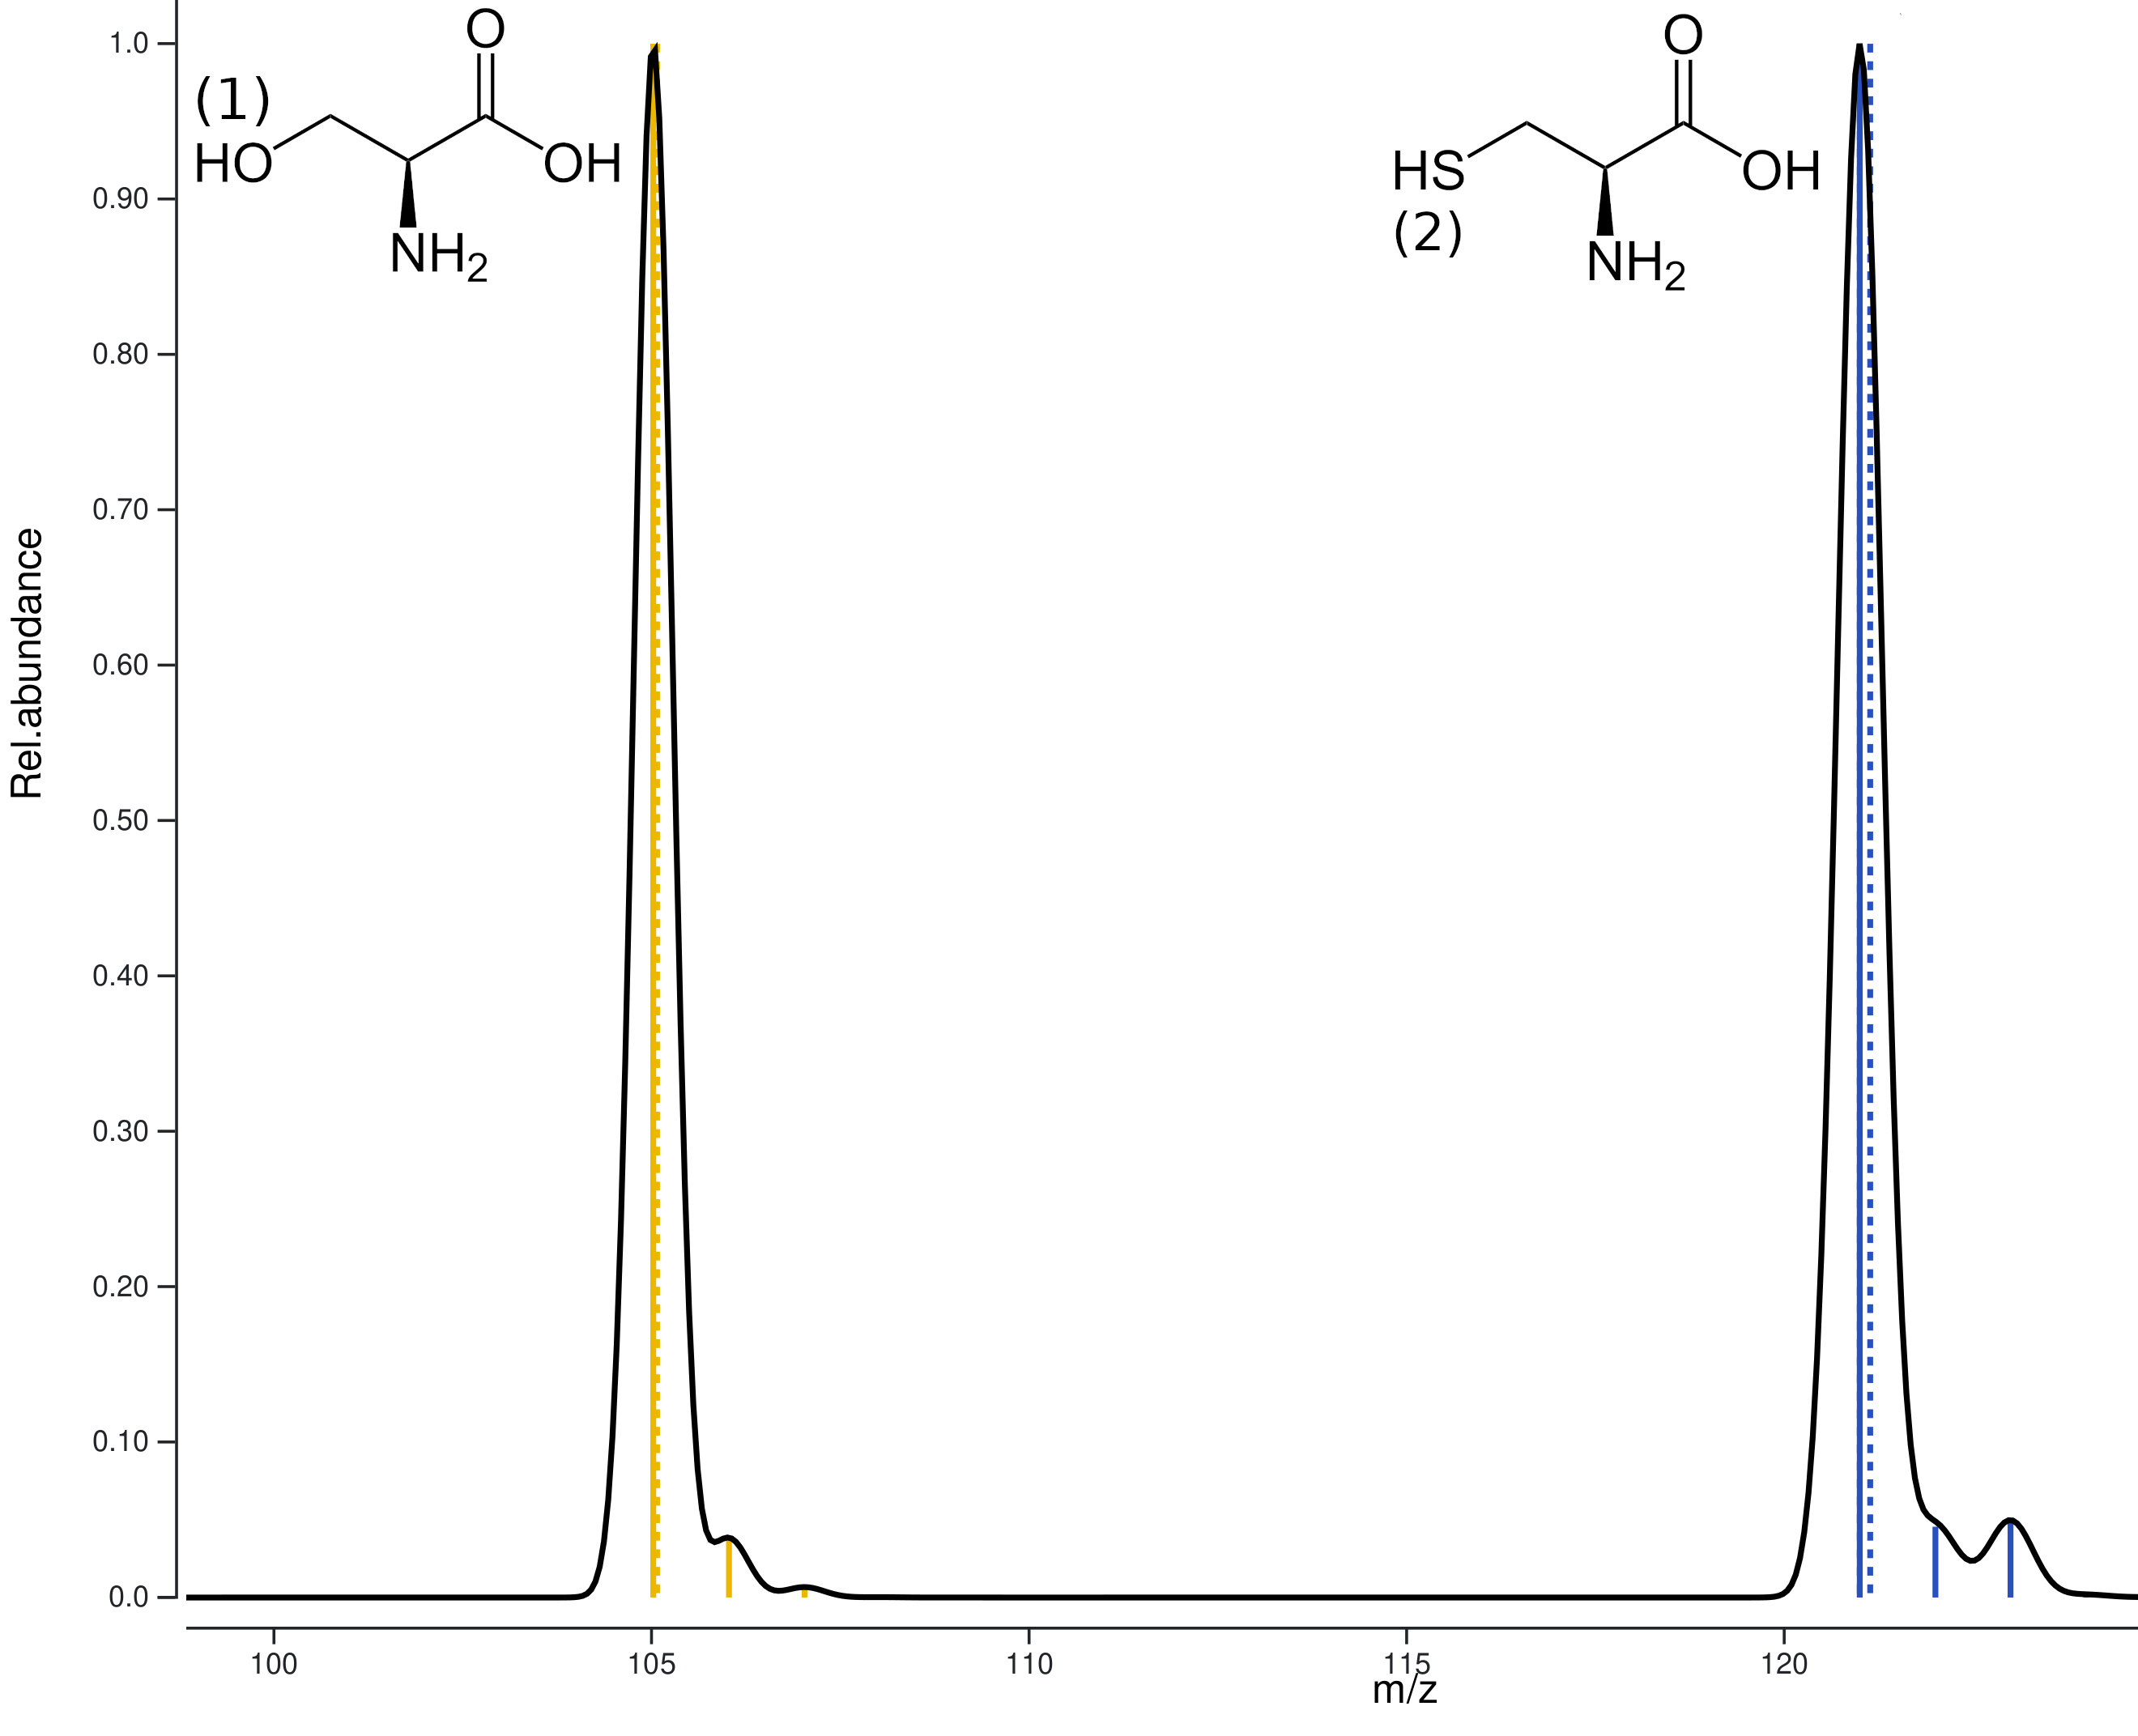
\includegraphics[width=0.75\textwidth]{./Resources/Simulated_Mass_Spectrum.png}
   \centering
   \caption{Computergeneriertes Massenspektrum von der Aminosäure \emph{Serin} (1) und \emph{Cystesin} (2). Peak von \emph{Serin} liegt bei 105; bei \emph{Systesin} um 121. y: relative Häufigkeit}
\end{figure}

Die Maxima werden \gerquot{Peaks} genannt und sind für eine Aminosäure an charakteristischer Position auf der $ x $-Achse. Obwohl sich die beiden Aminosäuren in der Abbildung \ref{fig:Sim_Mass_Spec} nur durch ein Atom unterscheiden (das linke Sauerstoffatom wurde durch ein Schwefelatom ersetzt) sind deren Massenspektren auf der $ x $-Achse weit voneinander entfernt und machen die beiden Aminosäuren dadurch sicher unterscheidbar.\\

Bei einzelnen Aminosäuren funktioniert die MS zuverlässig; bei Peptiden allerdings steht man vor dem Problem, dass das Massenspektrum unübersichtlicher wird und auch Peaks, die von Hintergrundrauschen stammen, schwerer herausgefiltert werden können. Abhilfe schafft hier die Tandem-Massenspektrometrie.

\subsection{Tandem-Massenspektrometrie (MS/MS)}\label{ss:Tandem_MS}
Bei der Tandem-Massenspektrometrie (MS/MS oder MS2) werden zwei MS Vorgänge hintereinander mit einer Probe durchgeführt. Die erste MS dient dazu Ionen aus einem bestimmten \massCharge Bereich auswählbar zu machen. Es entspricht also quasi einer Form der Filterung.

Vor der 2. MS werden die ausgewählten Reste einer Fragmentierung unterzogen. Bei einer Fragmentierung führt man Energie zu mit dem Ziel, dass die Ionen zerfallen und sog. Fragment-Ionen bilden. Diese Fragment-Ionen werden dann auf dem Massenspektrum nach der 2. MS sichtbar gemacht.

Fragment-Ionen sind kleiner als die ursprünglichen Ionen. So kann die 2. MS mit einer höheren Selektivität durchgeführt werden, welches Peaks durch Hintergrundrauschen verringert. Auch lassen sich Ionen besser identifizieren, die ein sehr ähnliches \massCharge-Verhältnis besitzen. Nach der 2. MS liegt eine Fülle an Fragment-Ionen-Peaks vor, aus denen sich die ursprünglichen Strukturinformationen ableiten lassen, da Ionen in spezifische Fragmente zerfallen \cite{Gross2013}. Zusammengefasst kann man sagen, dass das MS/MS Verfahren Ergebnisse höherer Güte erzeugt im Vergleich zur einfachen MS.

\section{De-Novo-Peptidsequenzierung mit \emph{pNovo+}}\label{s:pNovoPlusSeq}
Die \emph{pNovo+} Methode ist eine \gls{gls:DeNovo}, die mit einem \gls{gls:SpecGraph}en für die Auswertung der MS2-Spektren arbeitet und eine Erweiterung des \emph{pNovo} Verfahren darstellt \cite{pNovo}. Der Hauptansatz ist, dass zwei MS/MS Durchläufe mit jeweils verschiedenen Fragmentierungsmethoden\footnote{\emph{pNovo+} verwendet die higher energy
collisional dissociation (HCD) und die electron transfer dissociation (ETD) Fragmentierungsmethoden.} durchgeführt werden. Durch die Wahl einer anderen Fragmentierungsmethode ändert sich auch das MS2-Spektrum. Wenn nun Fragmentierungsmethoden verwendet werden, die möglichst komplementäre Spektren erzeugen, dann lässt sich durch das Zusammenführen der beiden MS2-Spektren die Qualität der Ergebnisse verbessern. Zum Beispiel lassen sich dadurch viele Peaks, die vom Hintergrundrauschen stammen, entfernen.

Für die Ermittlung der Sequenz eines Peptides wird zunächst ein Spektrums-Graph gebildet \dashAndSpace in Form eines DAG (directed acyclic graph). In diesem Graphen wird dann der längste Pfad bei gegebenen Start- und Endknoten berechnet. Die Reihenfolge der Knoten, die im längsten Pfad durchlaufen werden, stellt dann die Peptidsequenz dar.

\subsection{Vorverarbeitung der MS2-Spektren}\label{ss:Vorverarbeitung}
Bevor aus den MS2-Spektren der Spektrums-Graph gebildet werden kann, müssen die Daten vorverarbeitet werden. Für die Auswertung ist es von entscheidener Bedeutung, dass möglichst wenig Peaks verwendet werden, die vom Hintergrundrauschen stammen. Im weiteren Verlauf werden an einem exemplarischen MS2-Spektrum die Verarbeitungsschritte dargestellt.\\

Der erste Schritt ist das Verwenden des natürlichen Logarithmus der Intensitäten. Die Idee dabei ist, dass Hintergrundrauschen nicht überpriorisiert wird.

\begin{figure}[H]
   \centering
   \begin{minipage}[t]{.45\linewidth}
      \centering
      \begin{tikzpicture}[scale=\tikzScale, baseline=(current bounding box.center)]
         \draw [<->,thick] (0,\yAxisHeight) node (yaxis) [above] {\yAxisUnit}
         |- (\xAxisLength,0) node (xaxis) [right] {\xAxisUnit};
\draw[thick] (0.2, 0.0) -- (0.2, 2.3);
\draw[thick] (0.382, 0.0) -- (0.382, 1.7);
\draw[thick] (0.476, 0.0) -- (0.476, 2.7);
\draw[thick] (0.456, 0.0) -- (0.456, 1.8);
\draw[thick] (0.6859999999999999, 0.0) -- (0.6859999999999999, 2.7);
\draw[thick] (0.6839999999999999, 0.0) -- (0.6839999999999999, 1.8);
\draw[thick] (0.752, 0.0) -- (0.752, 1.1);
\draw[thick] (0.8200000000000001, 0.0) -- (0.8200000000000001, 2.2);
\draw[thick] (1.076, 0.0) -- (1.076, 1.5);
\draw[thick] (1.16, 0.0) -- (1.16, 1.9);
\draw[thick] (1.2120000000000002, 0.0) -- (1.2120000000000002, 2.0);
\draw[thick] (1.28, 0.0) -- (1.28, 1.9);
\draw[thick] (1.452, 0.0) -- (1.452, 1.3);
\draw[thick] (1.426, 0.0) -- (1.426, 1.9);
\draw[thick] (1.548, 0.0) -- (1.548, 1.9);
\draw[thick] (1.6740000000000002, 0.0) -- (1.6740000000000002, 1.5);
\draw[thick] (1.788, 0.0) -- (1.788, 2.5);
\draw[thick] (1.856, 0.0) -- (1.856, 2.3);
\draw[thick] (2.036, 0.0) -- (2.036, 1.7);
\draw[thick] (2.142, 0.0) -- (2.142, 1.6);
\draw[thick] (2.2520000000000002, 0.0) -- (2.2520000000000002, 2.0);
\draw[thick] (2.386, 0.0) -- (2.386, 1.6);
\draw[thick] (2.488, 0.0) -- (2.488, 2.9);
\draw[thick] (2.4739999999999998, 0.0) -- (2.4739999999999998, 2.7);
\draw[thick] (2.504, 0.0) -- (2.504, 2.0);
\draw[thick] (2.682, 0.0) -- (2.682, 2.0);
\draw[thick] (2.702, 0.0) -- (2.702, 2.5);
\draw[thick] (2.9259999999999997, 0.0) -- (2.9259999999999997, 2.8);
\draw[thick] (3.024, 0.0) -- (3.024, 2.4);
\draw[thick] (3.096, 0.0) -- (3.096, 1.8);
\draw[thick] (3.244, 0.0) -- (3.244, 2.6);
\draw[thick] (3.362, 0.0) -- (3.362, 1.9);
\draw[thick] (3.46, 0.0) -- (3.46, 2.3);
\draw[thick] (3.516, 0.0) -- (3.516, 1.1);
\draw[thick] (3.584, 0.0) -- (3.584, 1.8);
\draw[thick] (3.652, 0.0) -- (3.652, 2.0);
\draw[thick] (3.838, 0.0) -- (3.838, 1.5);
\draw[thick] (3.8819999999999997, 0.0) -- (3.8819999999999997, 2.6);
\draw[thick] (4.088, 0.0) -- (4.088, 2.6);
\draw[thick] (4.046, 0.0) -- (4.046, 1.1);
\draw[thick] (4.167999999999999, 0.0) -- (4.167999999999999, 2.0);
\draw[thick] (4.266, 0.0) -- (4.266, 2.4);
\draw[thick] (4.38, 0.0) -- (4.38, 1.1);
\draw[thick] (4.456, 0.0) -- (4.456, 2.2);
\draw[thick] (4.644, 0.0) -- (4.644, 2.6);
\draw[thick] (4.675999999999999, 0.0) -- (4.675999999999999, 2.5);
\draw[thick] (4.898000000000001, 0.0) -- (4.898000000000001, 1.2);
   \end{tikzpicture}%
   \end{minipage}%
   \textbf{$\rightarrow$} 
   \begin{minipage}[t]{.45\linewidth}
      \centering
      \begin{tikzpicture}[scale=\tikzScale, baseline=(current bounding box.center)]
      \draw [<->,thick] (0,\yAxisHeight) node (yaxis) [above] {\yAxisUnit}
      |- (\xAxisLength,0) node (xaxis) [right] {\xAxisUnit};
\draw[thick] (0.2, 0.0) -- (0.2, {ln(2.3)});
\draw[thick] (0.382, 0.0) -- (0.382, {ln(1.7)});
\draw[thick] (0.476, 0.0) -- (0.476, {ln(2.7)});
\draw[thick] (0.456, 0.0) -- (0.456, {ln(1.8)});
\draw[thick] (0.6859999999999999, 0.0) -- (0.6859999999999999, {ln(2.7)});
\draw[thick] (0.6839999999999999, 0.0) -- (0.6839999999999999, {ln(1.8)});
\draw[thick] (0.752, 0.0) -- (0.752, {ln(1.1)});
\draw[thick] (0.8200000000000001, 0.0) -- (0.8200000000000001, {ln(2.2)});
\draw[thick] (1.076, 0.0) -- (1.076, {ln(1.5)});
\draw[thick] (1.16, 0.0) -- (1.16, {ln(1.9)});
\draw[thick] (1.2120000000000002, 0.0) -- (1.2120000000000002, {ln(2.0)});
\draw[thick] (1.28, 0.0) -- (1.28, {ln(1.9)});
\draw[thick] (1.452, 0.0) -- (1.452, {ln(1.3)});
\draw[thick] (1.426, 0.0) -- (1.426, {ln(1.9)});
\draw[thick] (1.548, 0.0) -- (1.548, {ln(1.9)});
\draw[thick] (1.6740000000000002, 0.0) -- (1.6740000000000002, {ln(1.5)});
\draw[thick] (1.788, 0.0) -- (1.788, {ln(2.5)});
\draw[thick] (1.856, 0.0) -- (1.856, {ln(2.3)});
\draw[thick] (2.036, 0.0) -- (2.036, {ln(1.7)});
\draw[thick] (2.142, 0.0) -- (2.142, {ln(1.6)});
\draw[thick] (2.2520000000000002, 0.0) -- (2.2520000000000002, {ln(2.0)});
\draw[thick] (2.386, 0.0) -- (2.386, {ln(1.6)});
\draw[thick] (2.488, 0.0) -- (2.488, {ln(2.9)});
\draw[thick] (2.4739999999999998, 0.0) -- (2.4739999999999998, {ln(2.7)});
\draw[thick] (2.504, 0.0) -- (2.504, {ln(2.0)});
\draw[thick] (2.682, 0.0) -- (2.682, {ln(2.0)});
\draw[thick] (2.702, 0.0) -- (2.702, {ln(2.5)});
\draw[thick] (2.9259999999999997, 0.0) -- (2.9259999999999997, {ln(2.8)});
\draw[thick] (3.024, 0.0) -- (3.024, {ln(2.4)});
\draw[thick] (3.096, 0.0) -- (3.096, {ln(1.8)});
\draw[thick] (3.244, 0.0) -- (3.244, {ln(2.6)});
\draw[thick] (3.362, 0.0) -- (3.362, {ln(1.9)});
\draw[thick] (3.46, 0.0) -- (3.46, {ln(2.3)});
\draw[thick] (3.516, 0.0) -- (3.516, {ln(1.1)});
\draw[thick] (3.584, 0.0) -- (3.584, {ln(1.8)});
\draw[thick] (3.652, 0.0) -- (3.652, {ln(2.0)});
\draw[thick] (3.838, 0.0) -- (3.838, {ln(1.5)});
\draw[thick] (3.8819999999999997, 0.0) -- (3.8819999999999997, {ln(2.6)});
\draw[thick] (4.088, 0.0) -- (4.088, {ln(2.6)});
\draw[thick] (4.046, 0.0) -- (4.046, {ln(1.1)});
\draw[thick] (4.167999999999999, 0.0) -- (4.167999999999999, {ln(2.0)});
\draw[thick] (4.266, 0.0) -- (4.266, {ln(2.4)});
\draw[thick] (4.38, 0.0) -- (4.38, {ln(1.1)});
\draw[thick] (4.456, 0.0) -- (4.456, {ln(2.2)});
\draw[thick] (4.644, 0.0) -- (4.644, {ln(2.6)});
\draw[thick] (4.675999999999999, 0.0) -- (4.675999999999999, {ln(2.5)});
\draw[thick] (4.898000000000001, 0.0) -- (4.898000000000001, {ln(1.2)});
      \end{tikzpicture}
      \end{minipage}
      \caption{Anwendung des $ ln $ auf einem exemplarischen MS2-Spektrum.}
\end{figure}

Für das Verständnis des nächsten Schrittes muss man sich in Erinnerung rufen, dass eine gleiche Aminosäure keineswegs immer die gleiche Masse hat. Durch Isotope existiert eine gewisse \gerquot{Massenbandbreite} für ein und dieselbe Aminosäure. MS Systeme sind heute so genau, dass sie diese Differenzen erkennen. Dies hat den ungewollten Effekt, dass mehrere Peaks zu einer Aminosäure gehören können \cite{IsotopicDistributionMS}. Gleichzeitig können die \gerquot{Massenbandbreiten} zweier Aminosäuren sich überschneiden, sodass im ungünstigen Fall zwei Peaks kaum unterscheidbar nebeneinander liegen.\\

Eine Möglichkeit mit dieser Problematik umzugehen ist die Verwendung der monoisotopischen Masse. Die monoisotopische Masse ist die \gerquot{[...] exact mass of the most abundant naturally occurring stable isotope determined relative to the mass of 12 C, which is assigned the exact value of 12.0000.} \cite{MonoisotopicMass}. Ohne dabei jetzt tiefer ins Detail zu gehen kann man sagen, dass alle Peaks, deren Intensität mit einer möglichen monoisotopischen Masse übereinstimmen, auf jeden Fall einer Aminosäure entsprechen und (höchstwahrscheinlich)\footnote{Natürlich ist es möglich, dass das Rauschen zufällig einer monoisotopischen Masse entspricht. Die Wahrscheinlichkeit dafür ist allerdings sehr gering.} kein Hintergrundrauschen sind \cite{MassDefectMS}. Diese Peaks bekommen eine sogennante \emph{charge state}.\\

Der Algorithmus verwendet die \emph{charge state} Peaks als Ausganspunkte für weitere Berechnungen. Wenn die \massCharge Differenz zu einem anderen Peak einem Peptidfragment entspricht, dann stammt dieser Peak höchstwahrscheinlich von einem Fragment. Insgesamt werden damit die relevanten Peptidfragmente herausgeholt. Abbildung \ref{MonoisotopicMassFiltering} zeigt das Ergebnis nach den beiden zuvor genannten Schritten.

\begin{figure}[H]\label{MonoisotopicMassFiltering}
   \centering
   \begin{minipage}[t]{.45\linewidth}
      \centering
      \begin{tikzpicture}[scale=\tikzScale, baseline=(current bounding box.center)]
         \draw [<->,thick] (0,\yAxisHeight) node (yaxis) [above] {\yAxisUnit}
         |- (\xAxisLength,0) node (xaxis) [right] {\xAxisUnit};
\draw[thick] (0.2, 0.0) -- (0.2, {ln(2.3)});
\draw[color=blue!85!,opacity=.55,thick] (0.382, 0.0) -- (0.382, {ln(1.7)});
\draw[color=blue!85!,opacity=.55,thick] (0.476, 0.0) -- (0.476, {ln(2.7)});
\draw[color=magenta,thick] (0.456, 0.0) -- (0.456, {ln(1.8)});
\draw[color=blue!85!,opacity=.55,thick] (0.6859999999999999, 0.0) -- (0.6859999999999999, {ln(2.7)});
\draw[color=blue!85!,opacity=.55,thick] (0.6839999999999999, 0.0) -- (0.6839999999999999, {ln(1.8)});
\draw[thick] (0.752, 0.0) -- (0.752, {ln(1.1)});
\draw[thick] (0.8200000000000001, 0.0) -- (0.8200000000000001, {ln(2.2)});
\draw[thick] (1.076, 0.0) -- (1.076, {ln(1.5)});
\draw[thick] (1.16, 0.0) -- (1.16, {ln(1.9)});
\draw[thick] (1.2120000000000002, 0.0) -- (1.2120000000000002, {ln(2.0)});
\draw[thick] (1.28, 0.0) -- (1.28, {ln(1.9)});
\draw[color=blue!85!,opacity=.55,thick] (1.452, 0.0) -- (1.452, {ln(1.3)});
\draw[color=blue!85!,opacity=.55,thick] (1.426, 0.0) -- (1.426, {ln(1.9)});
\draw[color=magenta,thick] (1.548, 0.0) -- (1.548, {ln(1.9)});
\draw[color=blue!85!,opacity=.55,thick] (1.6740000000000002, 0.0) -- (1.6740000000000002, {ln(1.5)});
\draw[color=blue!85!,opacity=.55,thick] (1.788, 0.0) -- (1.788, {ln(2.5)});
\draw[thick] (1.856, 0.0) -- (1.856, {ln(2.3)});
\draw[thick] (2.036, 0.0) -- (2.036, {ln(1.7)});
\draw[thick] (2.142, 0.0) -- (2.142, {ln(1.6)});
\draw[thick] (2.2520000000000002, 0.0) -- (2.2520000000000002, {ln(2.0)});
\draw[thick] (2.386, 0.0) -- (2.386, {ln(1.6)});
\draw[color=blue!85!,opacity=.55,thick] (2.488, 0.0) -- (2.488, {ln(2.9)});
\draw[thick] (2.4739999999999998, 0.0) -- (2.4739999999999998, {ln(2.7)});
\draw[color=blue!85!,opacity=.55,thick] (2.504, 0.0) -- (2.504, {ln(2.0)});
\draw[color=magenta,thick] (2.682, 0.0) -- (2.682, {ln(2.0)});
\draw[color=blue!85!,opacity=.55,thick] (2.702, 0.0) -- (2.702, {ln(2.5)});
\draw[thick] (2.9259999999999997, 0.0) -- (2.9259999999999997, {ln(2.8)});
\draw[thick] (3.024, 0.0) -- (3.024, {ln(2.4)});
\draw[thick] (3.096, 0.0) -- (3.096, {ln(1.8)});
\draw[thick] (3.244, 0.0) -- (3.244, {ln(2.6)});
\draw[thick] (3.362, 0.0) -- (3.362, {ln(1.9)});
\draw[color=blue!85!,opacity=.55,thick] (3.46, 0.0) -- (3.46, {ln(2.3)});
\draw[color=blue!85!,opacity=.55,thick] (3.516, 0.0) -- (3.516, {ln(1.1)});
\draw[color=blue!85!,opacity=.55,thick] (3.584, 0.0) -- (3.584, {ln(1.8)});
\draw[color=magenta,thick] (3.652, 0.0) -- (3.652, {ln(2.0)});
\draw[color=blue!85!,opacity=.55,thick] (3.838, 0.0) -- (3.838, {ln(1.5)});
\draw[color=blue!85!,opacity=.55,thick] (3.8819999999999997, 0.0) -- (3.8819999999999997, {ln(2.6)});
\draw[thick] (4.088, 0.0) -- (4.088, {ln(2.6)});
\draw[thick] (4.046, 0.0) -- (4.046, {ln(1.1)});
\draw[thick] (4.167999999999999, 0.0) -- (4.167999999999999, {ln(2.0)});
\draw[thick] (4.266, 0.0) -- (4.266, {ln(2.4)});
\draw[color=blue!85!,opacity=.55,thick] (4.38, 0.0) -- (4.38, {ln(1.1)});
\draw[color=blue!85!,opacity=.55,thick] (4.456, 0.0) -- (4.456, {ln(2.2)});
\draw[color=magenta,thick] (4.644, 0.0) -- (4.644, {ln(2.6)});
\draw[color=blue!85!,opacity=.55,thick] (4.675999999999999, 0.0) -- (4.675999999999999, {ln(2.5)});
\draw[color=blue!85!,opacity=.55,thick] (4.898000000000001, 0.0) -- (4.898000000000001, {ln(1.2)});
   \end{tikzpicture}%
   \end{minipage}%
   \textbf{$\rightarrow$} 
   \begin{minipage}[t]{.45\linewidth}
      \centering
      \begin{tikzpicture}[scale=\tikzScale, baseline=(current bounding box.center)]
      \draw [<->,thick] (0,\yAxisHeight) node (yaxis) [above] {\yAxisUnit}
      |- (\xAxisLength,0) node (xaxis) [right] {\xAxisUnit};
\draw[color=blue!85!,opacity=.55,thick] (0.382, 0.0) -- (0.382, {ln(1.7)});
\draw[color=blue!85!,opacity=.55,thick] (0.476, 0.0) -- (0.476, {ln(2.7)});
\draw[color=magenta,thick] (0.456, 0.0) -- (0.456, {ln(1.8)});
\draw[color=blue!85!,opacity=.55,thick] (0.6859999999999999, 0.0) -- (0.6859999999999999, {ln(2.7)});
\draw[color=blue!85!,opacity=.55,thick] (0.6839999999999999, 0.0) -- (0.6839999999999999, {ln(1.8)});
\draw[color=blue!85!,opacity=.55,thick] (1.452, 0.0) -- (1.452, {ln(1.3)});
\draw[color=blue!85!,opacity=.55,thick] (1.426, 0.0) -- (1.426, {ln(1.9)});
\draw[color=magenta,thick] (1.548, 0.0) -- (1.548, {ln(1.9)});
\draw[color=blue!85!,opacity=.55,thick] (1.6740000000000002, 0.0) -- (1.6740000000000002, {ln(1.5)});
\draw[color=blue!85!,opacity=.55,thick] (1.788, 0.0) -- (1.788, {ln(2.5)});
\draw[color=blue!85!,opacity=.55,thick] (2.488, 0.0) -- (2.488, {ln(2.9)});
\draw[color=blue!85!,opacity=.55,thick] (2.504, 0.0) -- (2.504, {ln(2.0)});
\draw[color=magenta,thick] (2.682, 0.0) -- (2.682, {ln(2.0)});
\draw[color=blue!85!,opacity=.55,thick] (2.702, 0.0) -- (2.702, {ln(2.5)});
\draw[color=blue!85!,opacity=.55,thick] (3.46, 0.0) -- (3.46, {ln(2.3)});
\draw[color=blue!85!,opacity=.55,thick] (3.516, 0.0) -- (3.516, {ln(1.1)});
\draw[color=blue!85!,opacity=.55,thick] (3.584, 0.0) -- (3.584, {ln(1.8)});
\draw[color=magenta,thick] (3.652, 0.0) -- (3.652, {ln(2.0)});
\draw[color=blue!85!,opacity=.55,thick] (3.838, 0.0) -- (3.838, {ln(1.5)});
\draw[color=blue!85!,opacity=.55,thick] (3.8819999999999997, 0.0) -- (3.8819999999999997, {ln(2.6)});
\draw[color=blue!85!,opacity=.55,thick] (4.38, 0.0) -- (4.38, {ln(1.1)});
\draw[color=blue!85!,opacity=.55,thick] (4.456, 0.0) -- (4.456, {ln(2.2)});
\draw[color=magenta,thick] (4.644, 0.0) -- (4.644, {ln(2.6)});
\draw[color=blue!85!,opacity=.55,thick] (4.675999999999999, 0.0) -- (4.675999999999999, {ln(2.5)});
\draw[color=blue!85!,opacity=.55,thick] (4.898000000000001, 0.0) -- (4.898000000000001, {ln(1.2)});
      \end{tikzpicture}
      \end{minipage}
      \caption{Entfernen von Peaks, die keiner monoisotopischen Masse entsprechen oder benachbart mit einer Differenz von einem Fragment-Ion sind.}
\end{figure}

Tatsächlich ist die Verarbeitung an dieser Stelle noch etwas komplexer. So existieren auch noch sogenannte \emph{isotopic cluster}\footnote{Definition eines \emph{isotopic cluster} nach IUPAC: \gerquot{Group of peaks representing ions of the same elemental composition, but different isotopic compositions.} \cite[1556]{IUPACDefinitions}}, die gesondert verarbeitet werden. Für das grundsätzliche Prinzip ist dieses Detail allerdings weniger relevant.\\

Im letzten Vorberarbeitungsschritt werden Peaks aus einem irrelevanten \massCharge Bereich entfernt und naheliegende Peaks werden zusammengefasst, indem der Mittelwert sowol des \massCharge Wertes als auch der der Intensität besimmt wird. Üblicherweise liegt der Bereich für das Zusammenfassen bei $ +- 20 ppm $.

\begin{figure}[H]
   \centering
   \begin{minipage}[t]{.45\linewidth}
      \centering
      \begin{tikzpicture}[scale=\tikzScale, baseline=(current bounding box.center)]
         \draw [<->,thick] (0,\yAxisHeight) node (yaxis) [above] {\yAxisUnit}
         |- (\xAxisLength,0) node (xaxis) [right] {\xAxisUnit};
\draw[thick] (0.382, 0.0) -- (0.382, {ln(1.7)});
\draw[thick] (0.476, 0.0) -- (0.476, {ln(2.7)});
\draw[thick] (0.456, 0.0) -- (0.456, {ln(1.8)});
\draw[thick] (0.6859999999999999, 0.0) -- (0.6859999999999999, {ln(2.7)});
\draw[thick] (0.6839999999999999, 0.0) -- (0.6839999999999999, {ln(1.8)});
\draw[color=red,thick] (1.452, 0.0) -- (1.452, {ln(1.3)});
\draw[color=red,thick] (1.426, 0.0) -- (1.426, {ln(1.9)});
\draw[thick] (1.548, 0.0) -- (1.548, {ln(1.9)});
\draw[thick] (1.6740000000000002, 0.0) -- (1.6740000000000002, {ln(1.5)});
\draw[thick] (1.788, 0.0) -- (1.788, {ln(2.5)});
\draw[color=red,thick] (2.488, 0.0) -- (2.488, {ln(2.9)});
\draw[color=red,thick] (2.504, 0.0) -- (2.504, {ln(2.0)});
\draw[color=red,thick] (2.682, 0.0) -- (2.682, {ln(2.0)});
\draw[color=red,thick] (2.702, 0.0) -- (2.702, {ln(2.5)});
\draw[thick] (3.46, 0.0) -- (3.46, {ln(2.3)});
\draw[thick] (3.516, 0.0) -- (3.516, {ln(1.1)});
\draw[thick] (3.584, 0.0) -- (3.584, {ln(1.8)});
\draw[thick] (3.652, 0.0) -- (3.652, {ln(2.0)});
\draw[color=red,thick] (3.838, 0.0) -- (3.838, {ln(1.5)});
\draw[color=red,thick] (3.8819999999999997, 0.0) -- (3.8819999999999997, {ln(2.6)});
\draw[thick] (4.38, 0.0) -- (4.38, {ln(1.1)});
\draw[thick] (4.456, 0.0) -- (4.456, {ln(2.2)});
\draw[thick] (4.644, 0.0) -- (4.644, {ln(2.6)});
\draw[thick] (4.675999999999999, 0.0) -- (4.675999999999999, {ln(2.5)});
\draw[thick] (4.898000000000001, 0.0) -- (4.898000000000001, {ln(1.2)});

\fill[red!25!,opacity=.25] (0,0) rectangle (1,\yAxisHeight-\axisColorOffset);
         \fill[red!25!,opacity=.25] (\xAxisLength-1,0) rectangle (\xAxisLength-\axisColorOffset,\yAxisHeight-\axisColorOffset);
         \fill[green!25!,opacity=.25] (1,0) rectangle (\xAxisLength-1,\yAxisHeight-\axisColorOffset);
   \end{tikzpicture}%
   \end{minipage}%
   \textbf{$\rightarrow$} 
   \begin{minipage}[t]{.45\linewidth}
      \centering
      \begin{tikzpicture}[scale=\tikzScale, baseline=(current bounding box.center)]
      \draw [<->,thick] (0,\yAxisHeight) node (yaxis) [above] {\yAxisUnit}
      |- (\xAxisLength,0) node (xaxis) [right] {\xAxisUnit};
%\draw[color=red,thick] (1.452, 0.0) -- (1.452, {ln(1.3)});
%\draw[color=red,thick] (1.426, 0.0) -- (1.426, {ln(1.9)});
\draw[color=red,ultra thick] ({(1.452+1.426)/2}, 0.0) -- ({(1.452+1.426)/2}, {(ln(1.3)+ln(1.9))/2});

\draw[thick] (1.548, 0.0) -- (1.548, {ln(1.9)});
\draw[thick] (1.6740000000000002, 0.0) -- (1.6740000000000002, {ln(1.5)});
\draw[thick] (1.788, 0.0) -- (1.788, {ln(2.5)});

%\draw[color=red,thick] (2.488, 0.0) -- (2.488, {ln(2.9)});
%\draw[color=red,thick] (2.504, 0.0) -- (2.504, {ln(2.0)});
\draw[color=red,ultra thick] ({(2.488+2.504)/2}, 0.0) -- ({(2.488+2.504)/2}, {(ln(2.9)+ln(2.0))/2});

%\draw[color=red,thick] (2.682, 0.0) -- (2.682, {ln(2.0)});
%\draw[color=red,thick] (2.702, 0.0) -- (2.702, {ln(2.5)});
\draw[color=red,ultra thick] ({(2.682+2.702)/2}, 0.0) -- ({(2.682+2.702)/2}, {(ln(2.0+ln(2.5))/2});

\draw[thick] (3.46, 0.0) -- (3.46, {ln(2.3)});
\draw[thick] (3.516, 0.0) -- (3.516, {ln(1.1)});
\draw[thick] (3.584, 0.0) -- (3.584, {ln(1.8)});
\draw[thick] (3.652, 0.0) -- (3.652, {ln(2.0)});

%\draw[color=red,thick] (3.838, 0.0) -- (3.838, {ln(1.5)});
%\draw[color=red,thick] (3.8819999999999997, 0.0) -- (3.8819999999999997,{ln(2.6)});
\draw[color=red,ultra thick] ({(3.838+3.8819999999999997)/2}, 0.0) -- ({(3.838+3.8819999999999997)/2}, {(ln(1.5)+ln(2.6))/2});

\fill[red!25!,opacity=.25] (0,0) rectangle (1,\yAxisHeight-\axisColorOffset);
         \fill[red!25!,opacity=.25] (\xAxisLength-1,0) rectangle (\xAxisLength-\axisColorOffset,\yAxisHeight-\axisColorOffset);
         \fill[green!25!,opacity=.25] (1,0) rectangle (\xAxisLength-1,\yAxisHeight-\axisColorOffset);
      \end{tikzpicture}
      \end{minipage}
      \caption{Entfernen von Peaks aus einem irrelevanten \massCharge Bereich und zusammenfassen naheliegender Peaks. Rot markierte Peaks sind jene, die zusammengefasst werden.}
\end{figure}

\subsection{Bildung eines Spektrums-Graphen}\label{ss:BildungSpekGraph}
Der Spektrums-Graph wird aus einem vorverarbeiteten MS2-Spektrum (siehe Kapitel: \ref{ss:Vorverarbeitung}) gebildet. Im initialen Zustand werden die Peaks als Knoten interpretiert. Dazu kommt ein Start- und Endknoten. Jedem Knoten wird eine Masse zugeordet; im initialen Zustand bekommt der Startknoten die Masse 0 und der Endknoten die Masse des vorherigen Knotens minus der Masse des Wassers ($ 18,02 $). Die Masse der übrigen Knoten entsprechen ihren jeweils korrespondierenden \massCharge Wert. Die gerichteten Kanten werden zwischen einem Knotenpaar hinzugefügt, wenn die Differenz deren Masse gleich ist mit der Masse von ein oder zwei Aminosäuren.

\subsection{Identifikation der Aminosäuresequenz}
Der gebildete DAG kann mit klassischen Algorithmen, die den längsten Pfad suchen, durchlaufen werden. Bezogen auf die Graphentheorie entspricht die Ermittlung der Aminosäurensequenz dem Suchen eines bestimmten Pfades \dashAndSpace und nicht nach irgendeinem Pfad. Daher muss der Algorithmus mittels einer Breitensuche arbeiten, um alle möglichen Pfade zu bestimmen.

In aller Regel wird es mehrere Pfade geben. Bestimmte Sequenzen sind wahrscheinlicher als andere. So sind Pfade mit Kanten, die wegen der Massendifferenz von genau einer Aminosäure gebildet wurden, wahrscheinlicher \cite{pNovoPlus}. Alle Pfade bekommen mittels einer Scoring-Funktion einen Wert zugewiesen. Der Pfad mit dem höchsten Scoring-Wert ist wahrscheinlich das richtige Ergebnis. Die Scoring-Funktion berücksichtigt unter anderem wie viele Fragmente, die einer bestimmten Aminosäure zugeordet werden können, im MS2-Spektrum vorhanden sind \cite{pNovo}. Die Sequenz mit dem höchsten Scoring-Wert ist das Endergebnis.

\section{De-Novo-Peptidsequenzierung mit \emph{Open-pNovo}}\label{s:OpenpNovoSeq}
Bei Proteinen können posttranslationale Proteinmodifikationen (PTM) auftreten. PTMs sind Ereignisse, bei denen sich Änderungen im Protein einstellen \cite{Mann2003}; teilweise sind die Änderungen von einer Zelle erwünscht \dashAndSpace teilweise stammen sie aber auch zum Beispiel von unerwünschten Wechselwirkungen nebeneinanderliegenden Aminosäuren. Ein Teil dieser PTMs führen zu einer Änderung der Aminosäuresequenz. Dies ist für die \gls{gls:DeNovo} nicht weiter problematisch, da sowieso ohne eine Datenbank gearbeitet wird, sodass solche PTMs nicht einmal auffallen würden. Andere PTMs hingegen haben die Auswirkung, dass Stoffe gebildet werden, die nicht mehr zu der Gruppe der proteinogenen Aminosäuren gehören. Proteinogene Aminosäuren sind jene Aminosäuren, die für den Bau von Proteinen verwendet werden. Der Effekt ist also, dass Stoffe (oder deren Fragmente) bei einem Massenspektrum angezeigt werden, die kein Teil eines Peptids sein können. Bei der Sequenzierung von Peptidfragmenten muss dies daher berücksichtigt werden.
Wenn im weiteren Verlauf von PTMs gesprochen wird, dann sind solche gemeint, die für die \gls{gls:DeNovo} relevant sind.

Open-pNovo ist ein \gls{gls:DeNovo}sverfahren, welches auf pNovo+ Tool aufbaut und versucht die Problematik mit den PTMs zu lösen.

\subsection{PTMs im konstruierten DAG}
Die Konvertierung eines MS2-Spektrums läuft bis zum DAG analog ab wie in den Kapiteln \ref{ss:Vorverarbeitung} und \ref{ss:BildungSpekGraph} für pNovo+. Der Unterschied ist nun, dass es zwei Arten von Kanten gibt:

\begin{itemize}
   \item \gerquot{Normale} Kanten: Kanten, die gebildet werden, wie es bereits für \emph{pNovo+} gezeigt wurde. 
   \item \gerquot{Modifizierte} Kanten: Kanten, die zum Grahpen hinzugefügt werden, wenn die Massendifferenz zweier Knoten der Masse einer Aminosäure plus der Masse einer möglichen PTM-Änderung entspricht. 
\end{itemize}

Eine Liste aller PTMs in der Datenbank Unimod (sowohl relevante als auch nicht relevante) beinhaltet aktuell 1510 Einträge\footnote{Siehe: \url{https://www.ebi.ac.uk/ols/ontologies/unimod}} (Stand: 18.04.2022). Für die modifizierten Kanten gibt es insgesamt $ 1510 * 20 = 30200 $ mögliche Differenzen, wobei viele davon nicht relevante PTMs sind. Zum Vergleich: bei den normalen Kanten gibt es $ 20^2 = 400 $ mögliche Differenzen.

Die hohe Anzahl an Differenzen für modifizierte Kanten hat die Konsequenz, dass viele Knoten zufällig verbunden werden und dass dadurch die Genauigkeit der Ergebnisse abnimmt. Dieses Problem kann man durch eine geringere Liste an möglichen PTMs abfedern, allerdings mit einem Verlust  der Genauigkeit auf Seiten der PTMs. Es ist hier also eine Abwägung.

\subsection{Evaluierung von Open-pNovo}
Open-pNovo wurde sowohl auf drei realen als auch auf drei generierten Testdaten getestet. Tabelle \ref{tab:OpenPNovoResults} zeigt die Ergebnisse im Vergleich zu pNovo+ und zwei anderen Algorithmen. Die Datensätze enthielten die am häufigsten vorkommenden PTMs.

\begin{table}[H]
    \centering
    \begin{tabular}{l|c|c|c|c}
        \toprule
        \textbf{Testdatensätze} & \textbf{Open-pNovo+} & \textbf{pNovo+} & \textbf{PEAKS} & \textbf{Novor} \\
        \midrule
        Real (20259) & $76,3 \%$ & $68,5 \%$ & $65,8 \%$ & $39,9 \%$ \\
        Generiert (17877) & $77,8 \%$ & $0,6 \%$ & $0,5 \%$ & $0,2 \%$ \\
        \bottomrule
    \end{tabular}
    \newline
    \caption{Vergleich der durchschnittlichen richtigen \gls{gls:DeNovo} Peptidsequenzierungen von Open-pNovo und anderen Algorithmen \cite[650]{OpenPNovo}.}
    \label{tab:OpenPNovoResults}
\end{table}

Die enorm schlechten Ergebnisse der anderen Algorithmen bei den generierten Testdaten ist ein Nebeneffekt des Ziels bei der Testdatengenerierung. Denn diese wurden so ausgelegt, um die Grenzen von Open-pNovo+ zu ermitteln \cite[649]{OpenPNovo}. Eine Aussagekraft haben diese Ergebnisse also nicht. Allerdings auch bei realen Testdaten zeigt sich Open-pNovo als voll konkurrenzfähig gegenüber den anderen Algorithmen.

Noch besser zeigt sich Open-pNovo, wenn der Recall Wert betrachtet wird \dashAndSpace also die Anzahl an verschiedenen PSMs, die erkannt wurden. In diesem Fall ist der Abstand zu den anderen Algorithmen deutlich größer geworden.

\begin{table}[H]
    \centering
    \begin{tabular}{l|c|c|c|c}
        \toprule
        \textbf{Testdatensätze} & \textbf{Open-pNovo+} & \textbf{pNovo+} & \textbf{PEAKS} & \textbf{Novor} \\
        \midrule
        Real (5034) & $61,6 \%$ & $31,3 \%$ & $32,0 \%$ & $13,7 \%$ \\
        \bottomrule
    \end{tabular}
    \newline
    \caption{Vergleich der durchschnittlichen Recall Werte einer \gls{gls:DeNovo} Peptidsequenzierungen von Open-pNovo und anderen Algorithmen \cite[650]{OpenPNovo}.}
    \label{tab:OpenPNovoResultsRecall}
\end{table}

\subsection{Zusammenfassung}


% Die \gls{gls:DeNovo} nutzt die sogenannte \gls{gls:TMassSpek} für die Bestimmung der Peptidsequenz. Dabei wird die physikalische Eigenschaft ausgenutzt, dass jedes Atom bzw. jedes Molekül \dashAndSpace wenn es einer \gls{gls:Ionisation} unterzogen wurde \dashAndSpace ein charakteristisches \gls{gls:MassSpek} besitzt. Das \gls{gls:MassSpek} stellt also eine Art \gerquot{Fingerabdruck} eines Moleküls dar und macht dieses ermittelbar.

% U.U. eine Beispielgrafik eines Massenspektrums hinzufuegen ...

\subsubsection{\glsentrytext{gls:TMassSpek} bei größeren Molekülen}
Bei größeren Molekülen (wie einem Protein) führt die \gls{gls:Ionisation} dazu, dass das Molekül in kleinere spezifische Ionen zerfällt (sog. Fragmentierung). Die Fragmentierungsinformationen einer \gls{gls:DeNovo} sind meist unvollständig, da fehlende Daten bei einem Fragmentierungsschritt die Güte des Endergebnisses negativ beeinflusst. Dies wird insbesondere dann ein Problem, wenn unbekannte Änderungen in einer Peptidsequenz vorhanden sind.

Um dieses Problem zu verringern können unterschiedliche Techniken parallel eingesetzt werden, welche verschiedene Fragmente erzeugen und daher auch verschiedenartige \glspl{gls:MassSpek} zur Folge haben.\footnote{Konkret: Es wird sowohl das \gls{acr:HCD} als auch das \gls{acr:ETD} Verfahren angewendet.}

\subsection{Datenaufbereitung}
Typischerweise betrachtet man die sog. \gerquot{\glspl{gls:Peak}} in den \glspl{gls:MassSpek}. Jeder \gls{gls:Peak} stellt ein unterschiedliches Ion dar. Dazu kommen Messungenauigkeiten sowie Hintergrundrauschen. Durch die hohe Anzahl an möglichen Ionen kann nicht ohne weiteres differenziert werden, welcher der \glspl{gls:Peak} von welchen Ionen erzeugt wurden und welche nicht.

% Frage an Dominik: Ist hier eine einfache Auflistung an Techniken für die Datenaufbereitung besser?
Der Algorithmus für die Datenaufbereitung berechnet den natürlichen Logarithmus von den Intensitäten der \glspl{gls:Peak}, um Hintergrundrauschen und Messungenauigkeiten nicht überzupriorisieren. Zusätzlich dazu werden \glspl{gls:Peak}, die in einem Toleranzbereich nebeneinander liegen, zusammengefasst. Am Ende werden die \glspl{gls:Peak} entfernt, bei denen bekannt ist, dass es sich nicht um relevante Ionen handeln kann. (z.B. \glspl{gls:Peak} von Isotopen)

\begin{figure}[H]
   \centering
   \begin{minipage}[t]{.4\linewidth}
      \centering
      \begin{tikzpicture}[scale=\tikzScale, baseline=(current bounding box.center)]
         \draw [<->,thick] (0,2.75) node (yaxis) [above] {\yAxisUnit}
         |- (3,0) node (xaxis) [right] {\xAxisUnit};

         \draw[thick] (0.2,0) -- (0.2,1.1);
         \draw[thick] (0.3,0) -- (0.3,1.6);
         \draw[thick] (0.6,0) -- (0.6,1.7);
         \draw[thick] (0.8,0) -- (0.8,1.2);
         \draw[thick] (1.0,0) -- (1.0,1.1);

         \draw[color=red,thick] (1.2,0) -- (1.2,2.65);
         \draw[thick] (1.4,0) -- (1.4,1.4);
         \draw[thick] (1.6,0) -- (1.6,1.2);
         \draw[thick] (1.8,0) -- (1.8,1.3);
         \draw[thick] (2.0,0) -- (2.0,1.8);

         \draw[thick] (1.1,0) -- (1.1,2.0);
         \draw[color=red,thick] (0.35,0) -- (0.35,2.25);
         \draw[thick] (1.9,0) -- (1.9,1.4);
         \draw[color=red,thick] (2.2,0) -- (2.2,2.6);
         \draw[thick] (2.5,0) -- (2.5,1.25);

         \draw[thick] (2.7,0) -- (2.7,1.1);
         \foreach \x in {1,...,6}
         {
            \draw[thick] (1.2+\x*0.05,0) -- (1.2+\x*0.05,1.0+\x*0.15);
         }
      \end{tikzpicture}%
      % \subcaption{Exemplarische Rohdaten}
   \end{minipage}%
   \textbf{$\rightarrow$}
   \begin{minipage}[t]{.4\linewidth}
      \centering
      \begin{tikzpicture}[scale=\tikzScale, baseline=(current bounding box.center)]
         \draw [<->,thick] (0,2.75) node (yaxis) [above] {\yAxisUnit}
         |- (3,0) node (xaxis) [right] {\xAxisUnit};

         \draw[thick] (0.2,0) -- (0.2,{ln(1.1)});
         \draw[thick] (0.3,0) -- (0.3,{ln(1.6)});
         \draw[thick] (0.6,0) -- (0.6,{ln(1.7)});
         \draw[thick] (0.8,0) -- (0.8,{ln(1.2)});
         \draw[thick] (1.0,0) -- (1.0,{ln(1.1)});

         \draw[color=red,thick] (1.2,0) -- (1.2,{ln(2.65)});
         \draw[thick] (1.4,0) -- (1.4,{ln(1.4)});
         \draw[thick] (1.6,0) -- (1.6,{ln(1.2)});
         \draw[thick] (1.8,0) -- (1.8,{ln(1.3)});
         \draw[thick] (2.0,0) -- (2.0,{ln(1.8)});

         \draw[thick] (1.1,0) -- (1.1,{ln(2.0)});
         \draw[color=red,thick] (0.35,0) -- (0.35,{ln(2.25)});
         \draw[thick] (1.9,0) -- (1.9,{ln(1.4)});
         \draw[color=red,thick] (2.2,0) -- (2.2,{ln(2.6)});
         \draw[thick] (2.5,0) -- (2.5,{ln(1.25)});

         \draw[thick] (2.7,0) -- (2.7,{ln(1.1)});
         \foreach \x in {1,...,6}
         {%
            \draw[thick] (1.2+\x*0.05,0) -- (1.2+\x*0.05,{ln(1.0+\x*0.15)});
         }
      \end{tikzpicture}
      %\subcaption{Exemplarische Rohdaten}
   \end{minipage}
   \caption{Anwendung des $ln$ auf Rohdaten. Rote \glspl{gls:Peak} stellen hier exemplarisch fehlerhafte Daten dar, die nach dem $ln$ reduziert wurden.}
\end{figure}

\begin{figure}[H]
   \centering
   \begin{minipage}[t]{.4\linewidth}
      \centering
      \begin{tikzpicture}[scale=\tikzScale, baseline=(current bounding box.center)]
         \draw [<->,thick] (0,2.75) node (yaxis) [above] {\yAxisUnit}
         |- (3,0) node (xaxis) [right] {\xAxisUnit};

         \draw[thick] (0.2,0) -- (0.2,{ln(1.1)});
         \draw[thick] (0.3,0) -- (0.3,{ln(1.6)});
         \draw[thick] (0.6,0) -- (0.6,{ln(1.7)});
         \draw[thick] (0.8,0) -- (0.8,{ln(1.2)});
         \draw[thick] (1.0,0) -- (1.0,{ln(1.1)});

         \draw[thick] (1.2,0) -- (1.2,{ln(2.65)});
         \draw[thick] (1.4,0) -- (1.4,{ln(1.4)});
         \draw[thick] (1.6,0) -- (1.6,{ln(1.2)});
         \draw[thick] (1.8,0) -- (1.8,{ln(1.3)});
         \draw[thick] (2.0,0) -- (2.0,{ln(1.8)});

         \draw[thick] (1.1,0) -- (1.1,{ln(2.0)});
         \draw[thick] (0.35,0) -- (0.35,{ln(2.25)});
         \draw[thick] (1.9,0) -- (1.9,{ln(1.4)});
         \draw[thick] (2.2,0) -- (2.2,{ln(2.6)});
         \draw[thick] (2.5,0) -- (2.5,{ln(1.25)});

         \draw[thick] (2.7,0) -- (2.7,{ln(1.1)});
         \foreach \x in {1,...,6}
         {%
            \draw[color=red,thick] (1.2+\x*0.05,0) -- (1.2+\x*0.05,{ln(1.0+\x*0.15)});
         }

         \draw[dotted] (0.4,0) -- (0.4,2.75);
         \draw[dotted] (2.6,0) -- (2.6,2.75);
         \fill[red!25!,opacity=.25] (0,0) rectangle (0.4,2.75);
         \fill[red!25!,opacity=.25] (2.6,0) rectangle (3.0,2.75);
         \fill[green!25!,opacity=.25] (0.4,0) rectangle (2.6,2.75);
      \end{tikzpicture}
      %\subcaption{Exemplarische Rohdaten}
   \end{minipage}
   \textbf{$\rightarrow$}
   \begin{minipage}[t]{.4\linewidth}
      \centering
      \begin{tikzpicture}[scale=\tikzScale, baseline=(current bounding box.center)]
         \draw [<->,thick] (0,2.75) node (yaxis) [above] {\yAxisUnit}
         |- (3,0) node (xaxis) [right] {\xAxisUnit};

         \draw[thick] (0.6,0) -- (0.6,{ln(1.7)});
         \draw[thick] (0.8,0) -- (0.8,{ln(1.2)});
         \draw[thick] (1.0,0) -- (1.0,{ln(1.1)});

         \draw[thick] (1.2,0) -- (1.2,{ln(2.65)});
         %\draw[thick] (1.4,0) -- (1.4,{ln(1.4)});
         \draw[thick] (1.6,0) -- (1.6,{ln(1.2)});
         \draw[thick] (1.8,0) -- (1.8,{ln(1.3)});
         \draw[thick] (2.0,0) -- (2.0,{ln(1.8)});

         \draw[thick] (1.1,0) -- (1.1,{ln(2.0)});
         \draw[thick] (1.9,0) -- (1.9,{ln(1.4)});
         \draw[thick] (2.2,0) -- (2.2,{ln(2.6)});
         \draw[thick] (2.5,0) -- (2.5,{ln(1.25)});

         \draw[color=red,ultra thick] (1.2+1*0.05,0) -- (1.2+1*0.05,{ln(1.0+1*0.15)});
         \draw[color=red,ultra thick] (1.2+3*0.05,0) -- (1.2+3*0.05,{ln(1.0+3*0.15)});
         \draw[color=red,ultra thick] (1.2+5*0.05,0) -- (1.2+5*0.05,{ln(1.0+5*0.15)});

         \draw[dotted] (0.4,0) -- (0.4,2.75);
         \draw[dotted] (2.6,0) -- (2.6,2.75);
         \fill[red!25!,opacity=.25] (0,0) rectangle (0.4,2.75);
         \fill[red!25!,opacity=.25] (2.6,0) rectangle (3.0,2.75);
         \fill[green!25!,opacity=.25] (0.4,0) rectangle (2.6,2.75);
      \end{tikzpicture}
      %\subcaption{Exemplarische Rohdaten}
   \end{minipage}
   \caption{Entfernen von irrelevanten \glspl{gls:Peak} sowie zusammenfassen naheliegender \glspl{gls:Peak}. Hier symbolisieren die roten \glspl{gls:Peak} jene, die zusammengefasst werden.}
\end{figure}

% `\glsentrytext` funktioniert nicht für `\glspl`
\subsection{Konvertierung von \glspl{gls:MassSpek}}
Das Ziel der Konvertierung ist das Erzeugen eines \gls{gls:SpecGraph}en. Um von einem \gls{gls:MassSpek} zu einem \gls{gls:SpecGraph}en zu kommen, werden die \glspl{gls:Peak}, die nach der Datenaufbereitung (Siehe ...) übrig bleiben, als Knoten gewertet. Dazu kommt ein Start- und Endknoten. Jeder Knoten bekommt eine Gewichtung; diese Gewichtung entspricht der Stärke des \gls{gls:Peak}s.

\newcommand{\colorA}{white!30!green}
\newcommand{\colorB}{black!10!yellow}
\newcommand{\colorC}{white!40!red}
\newcommand{\colorD}{white!25!orange}
\newcommand{\colorE}{white!45!blue}
\newcommand{\colorF}{white!5!magenta}
\newcommand{\nodeFontSize}{\scriptsize}
\newcommand{\nodeScaleFactor}{100}
\newcommand{\round}[1]{\pgfmathprintnumber[precision=0]{#1}}
\newcommand{\rawA}{ln(1.7)}
\newcommand{\rawB}{ln(2.0)}
\newcommand{\rawC}{ln(2.65)}
\newcommand{\rawD}{ln(1.0+5*0.15)}
\newcommand{\rawE}{ln(1.85)}
\newcommand{\rawF}{ln(2.6)}
\newcommand{\valueA}{\pgfmathparse{int(\rawA*\nodeScaleFactor)}\pgfmathresult}
\newcommand{\valueB}{\pgfmathparse{int(\rawB*\nodeScaleFactor)}\pgfmathresult}
\newcommand{\valueC}{\pgfmathparse{int(\rawC*\nodeScaleFactor)}\pgfmathresult}
\newcommand{\valueD}{\pgfmathparse{int(\rawD*\nodeScaleFactor)}\pgfmathresult}
\newcommand{\valueE}{\pgfmathparse{int(\rawE*\nodeScaleFactor)}\pgfmathresult}
\newcommand{\valueF}{\pgfmathparse{int(\rawF*\nodeScaleFactor)}\pgfmathresult}

\begin{figure}[htb]
   \centering
      \begin{tikzpicture}[scale=\tikzScale*1.5, baseline=(current bounding box.center)]
         \draw [<->,thick] (0,2.75) node (yaxis) [above] {\yAxisUnit}
         |- (3,0) node (xaxis) [below] {\xAxisUnit};

         \draw[thick] (0.6,0) -- (0.6,{ln(1.7)}) node [right, rotate=90, color=\colorA] {\nodeFontSize\textbf{A} \valueA};
         \draw[thick] (0.8,0) -- (0.8,{ln(1.2)});
         \draw[thick] (1.0,0) -- (1.0,{ln(1.1)});

         \draw[thick] (1.2,0) -- (1.2,{ln(2.65)}) node [right, rotate=90,
         color=\colorC] {\nodeFontSize\textbf{C} \valueC};
         \draw[thick] (1.4,0) -- (1.4,{ln(1.4)});
         \draw[thick] (1.6,0) -- (1.6,{ln(1.2)});
         \draw[thick] (1.8,0) -- (1.8,{ln(1.3)});
         \draw[thick] (2.0,0) -- (2.0,{ln(1.8)}) node [right, rotate=90, color=\colorE] {\nodeFontSize\textbf{E} \valueE};

         \draw[thick] (1.025,0) -- (1.025,{ln(2.0)}) node [right, rotate=90, color=\colorB] {\nodeFontSize\textbf{B} \valueB};
         \draw[thick] (1.9,0) -- (1.9,{ln(1.4)});
         \draw[thick] (2.2,0) -- (2.2,{ln(2.6)}) node [right, rotate=90, color=\colorF] {\nodeFontSize\textbf{F} \valueF};
         \draw[thick] (2.5,0) -- (2.5,{ln(1.25)});

         \draw[thick] (1.2+1*0.05,0) -- (1.2+1*0.05,{ln(1.0+1*0.15)});
         \draw[thick] (1.2+3*0.05,0) -- (1.2+3*0.05,{ln(1.0+3*0.15)});
         \draw[thick] (1.2+5*0.05,0) -- (1.2+5*0.05,{ln(1.0+5*0.15)}) node [right, rotate=90, color=\colorD] {\nodeFontSize\textbf{D} \valueD};
      \end{tikzpicture}
      \caption{Ausgewählte \glspl{gls:Peak} mit einem exemplarischen x Wert.}
\end{figure}

\newcommand{\modVal}{4}

Gerichtete Kanten zwischen den Knoten werden ausgebildet, wenn diese eine Differenz von genau einer oder zwei Aminosäurereste\footnote{Da eine Aminosäure vielerlei an Reste besitzen kann, ergeben sich mehr als 40 Differenzen, die diese Bedingung erfüllen.} besitzen. Der Einfachheit halber wird im folgenden eine Kante ausgebildet, wenn die Differenz genau \textbf{\modVal} \space beträgt.

% Um einzele Knotennamen einzufärben: \textcolor{\colorA}{A}
\newcommand{\findRaw}[1]{\csname raw#1\endcsname}
\newcommand{\findValue}[1]{\csname value#1\endcsname}
\newcommand{\findColor}[1]{\csname color#1\endcsname}
\newcommand{\cmark}{\ding{51}}
\newcommand{\xmark}{\ding{55}}
\newcommand{\tableRow}[2]
{%
   % Welche Zeile soll farblich hinterlegt werden ?
   \pgfmathparse{Mod(abs(int(\findRaw{#1}*\nodeScaleFactor) - int(\findRaw{#2}*\nodeScaleFactor)),\modVal)}
   \pgfmathtruncatemacro\myresult{\pgfmathresult==0.0?1:0}
   %\ifthenelse{\myresult=1}{A}{B}
   \ifnum\myresult=1 A \else B \fi

   (#1,#2) &
   \findValue{#1} &
   \findValue{#2} &
   \pgfmathparse{abs(int(\findRaw{#1}*\nodeScaleFactor) - int(\findRaw{#2}*\nodeScaleFactor))}\round{\pgfmathresult} &

   % Hilfreiche Infos für das Erstellen von Ausdrücken: https://tikz.dev/math-parsing
   \pgfmathparse{Mod(abs(int(\findRaw{#1}*\nodeScaleFactor) - int(\findRaw{#2}*\nodeScaleFactor)),\modVal)}
   % https://www.reddit.com/r/LaTeX/comments/57ck5p/tikz_which_conditionals_to_use_to_compare_numbers/
   \pgfmathtruncatemacro\myresult{\pgfmathresult==0.0?1:0}
   \round{\pgfmathresult}
   \ifthenelse{\myresult=1}{\cmark}{\xmark}
   \\
}
% Hilfestellung: https://tex.stackexchange.com/questions/604496/how-to-generate-beautiful-tables-in-latex
\begin{table}[H]
    \centering
    \begin{tabular}{lllcc}
        \toprule
        \thead{\textbf{$\mathbf{(u,v)}$}} & \thead{$\mathbf{u}$} & \thead{$\mathbf{v}$} & \thead{$\mathbf{\Delta(u,v)}$} & \thead{$\Delta(u,v)\bmod\modVal$}\\
        \midrule
        \tableRow{A}{B}
        \tableRow{A}{C}
        \tableRow{A}{D}
        \tableRow{A}{E}
        \tableRow{A}{F}
        \tableRow{B}{C}
        \tableRow{B}{D}
        \tableRow{B}{E}
        \tableRow{B}{F}
        \tableRow{C}{D}
        \tableRow{C}{E}
        \tableRow{C}{F}
        \tableRow{D}{E}
        \tableRow{D}{F}
        \tableRow{E}{F}
        \bottomrule
    \end{tabular}
    \caption{Bestimmung der Kanten}
\end{table}

Darstellung der Daten als gewichteter, gerichteter azyklischer Graph. Zusätzlich benötigt der Graph noch separate Start- und Zielknoten; diese sind für die späteren Berechnungen unerlässlich.

\newcommand{\printVertices}[2]%
{%
   \Vertex[x=-8,y=0]{Start}
   \Vertex[x=8,y=0]{End}
   \foreach \x [count=\xi] in {#1}
   {%
      \foreach \y [count=\yi] in {#2}
      {%
         \ifthenelse{\xi=\yi}{
         \tikzstyle{VertexStyle}=[shape=circle,fill=\y,draw=black,line width=0.75pt]
         \Vertex[x=-7+\xi*2,y=0]{\x}}{\break}
      }
   }
}
% https://tex.stackexchange.com/questions/245448/adjusting-edge-and-vertex-label
\begin{figure}[htb]
   \centering
   \begin{tikzpicture}[scale=0.75,transform shape]
      \tikzstyle{VertexStyle}=[shape=circle,fill=white,draw=black,line width=1pt]

      \printVertices{A,B,C,D,E,F}{\colorA, \colorB, \colorC, \colorD, \colorE, \colorF}

      \tikzstyle{LabelStyle}=[fill=white, sloped]
      \tikzstyle{EdgeStyle}=[bend left, post]
      \Edge[label=$0$](Start)(A)
      \Edge[label=$0$](F)(End)
      \tikzstyle{EdgeStyle}=[bend right, post]
      \Edge[label=$16$](A)(B)
      \tikzstyle{EdgeStyle}=[bend left, post]
      \Edge[label=$44$](A)(C)
      \Edge[label=$8$](A)(E)
      \tikzstyle{EdgeStyle}=[bend right, post]
      \Edge[label=$28$](B)(C)
      \Edge[label=$8$](B)(E)
      \Edge[label=$36$](C)(E)
      \tikzstyle{EdgeStyle}=[bend left, post]
      \Edge[label=$40$](D)(F)
   \end{tikzpicture}
   \caption{Erzeugter DAG}
\end{figure}

Bereits an diesem Minimalbeispiel ist zu erkennen, dass die gebildeten Knoten in einem \glspl{gls:SpecGraph} nur wenige ausgehende Kanten besitzen. Dies ist nicht dem Beispiel geschuldet sondern ist tatsächlich auch in der Praxis der Regelfall. Dies ist eine hilfreiche Beobachtung für die Datenauswertung (siehe Abschnitt~\ref{Datenauswertung} \gerquot{\titleref{Datenauswertung}}).


\subsection{Datenauswertung}\label{Datenauswertung}
Um nun aus dem Graphen die Peptidsequenz zu gewinnen müssen alle längsten Pfade im DAG gefunden werden. Da die Kanten gewichtet sind, kann es durchaus mehrere längste Pfade geben. Gleichwohl es Algorithmen für das Problem des längsten Pfades in einem Graphen gibt, handelt es sich hierbei um ein $NP$-schweres Problem. Es existiert also (wahrscheinlich) kein effizienter Algorithmus. Erschwerend kommt hinzu, dass der Graph nicht zwingend ein zusammenhängender Graph sein muss \dashAndSpace auch wenn dies meist der Fall ist. Der Graph muss daher vor Berechnungsbeginn auf diese Eigenschaft hin überprüft werden.

Im Falle der \glspl{gls:SpecGraph} existiert die Eigenschaft, dass solche Graphen meist eine geringe Dichte an Kanten aufweisen. Dies hat den positiven Effekt, dass die Anzahl an überhaupt möglichen längsten Pfaden recht gering ist. Zusätzlich dazu kann die Warteschlange, die in den longest Path DAG Algorithmen verwendet werden, angepasst werden. Da die Gewichtung der Kanten als eine Art \gerquot{Wahrscheinlichkeit}, dass die nächste Kante die reale Peptidsequenz darstellt, interpretiert werden kann, kann eine priorisierte Warteschlange verwendet werden, die die Laufzeit ebenfalls verbessert. In Summe führen diese Eigenschaften der \glspl{gls:SpecGraph} dazu, dass das längste Pfade Problem in solchen Fällen auf die Laufzeit $\mathcal{O}(abs(E) + log(d))$ reduziert werden kann.\\

Zusammengefasst: Es wird versucht die speziellen Eigenschaften der Graphen auszunutzen, um die Laufzeit zu verbessern.


\section{Ergebnisse/Evaluierung}
Im folgenden Kapitel werden die Probleme, die in der Praxis bei der Verwendung des Verfahrens auftreten, erläutert und mögliche Lösungsansätze aufgezeigt.

\subsection{Probleme in der Praxis}
\subsubsection{Qualität der Messwerte}
Obwohl eine Datenaufbereitung stattfindet, ist das Verfahren bei der Verwendung von \glspl{gls:SpecGraph} stark auf die Genauigkeit der Messwerte angewiesen. Zwar sind durch technische Fortschritte bei der \gls{gls:TMassSpek} die Daten hochwertiger geworden; dennoch gestaltet sich das Sequenzieren von unbekannten Peptidsequenzen als schwierig. Mit heutigen Gerätschaften lassen sich bei der Verwendung des genannten Verfahrens bis zu 13 Peptide mit einer durchschnittlichen Genauigkeit von 94\% ermitteln. Danach nimmt diese sprunghaft ab. Für brauchbare Ergebnisse wird \dashAndSpace je nach Literatur \dashAndSpace eine Trefferquote von 90-95\% vorausgesetzt.
\subsubsection{Fehlende Betrachtung der \glsentrytext{gls:StereoIsomerie}}\label{FehlendeStereoInfos}
Das komplette Verfahren basiert auf das Masse-Ladungs-Verhältnis, sodass Stereoinformationen schlicht nicht ermittelt werden können. Es kann zwar mithilfe einer energetischen Betrachtung bestimmt werden welche \glspl{gls:StereoIsomer} in welchen Verhältnis auftreten (müssten). Dabei handelt es sich allerdings lediglich um eine grobe Abschätzung.
\subsubsection{Identifikation der Aminosäuren über Massendifferenz}
Die Grundidee bei der Identifikation von Aminosäuren ist die Betrachtung der Massendifferenzen zwischen zwei \glspl{gls:Peak}. Zwar liefert dieser Ansatz häufig passende Ergebnisse. Dennoch ist solch eine Differenz nicht in der Lage jede Aminosäure immer eindeutig zu identifizieren, da bestimmte Kombinationen (fast) gleiche Differenzen besitzen. Der Algorithmus, der die Gewichtungen bestimmt, arbeitet nur mit ganzzahligen Werten. Dadurch gehen leichte Unterschiede, die durch die Isotope (insb. die des Kohlenstoffes) begründet sind, meist durch die Float Integer Konvertierung verloren.

\subsection{Lösungsansätze}
\subsubsection{Verbesserung der Ergebnisse durch Machine Learning}
Bei der Sequenzierung werden ab einer gewissen Länge unweigerlich Fehler eintreten.\cite[S.621,Figure 5]{pNovoPlus} Dadurch, dass nicht jede Peptidsequenz gleich wahrscheinlich ist\footnote{Dies ist u.a. dadurch begründet, dass die Reste der Aminosäuren sich gegenseitig beeinflussen (können), sodass bestimmte Sequenzen energetisch ungünstig sind und lediglich vermindert auftreten.}, können mittels Machine Learning grundsätzlich die Ergebnisse verbessert werden. insbesondere dann, wenn die ermittelte Differenz keinen eindeutigen Rückschluss auf die Aminosäure zulässt.

\section{Zusammenfassung}
Im letzten Kapitel werden die ungelösten Probleme genannt und erklärt warum diese eine Relevanz für die Praxis haben. Am Ende findet eine kritische Betrachtung des Verfahrens im allgemeinen statt.

\subsection{Ungelöste Probleme}
Wie bereits in \ref{FehlendeStereoInfos} erwähnt, kann das Verfahren designbedingt keine Stereoinformationen ermitteln. Daher ist es in diesem Fall besonders wichtig abzuschätzen, ob das Fehlen dieser Informationen tatsächlich eine Relevanz hat. Wenn nur die Peptidsequenz betrachtet werden soll, dann stellt dies kein Problem dar. Aber sobald jedweige Abschätzungen anhand der ermittelten Sequenz stattfinden soll, dann kann das Fehlen jener Informationen zu massiven Fehlern führen.\\

Wenn für die Verbesserung der Ergebnisse Machine Learning in Betracht kommt, dann muss dabei berücksichtigt werden, dass dadurch unter Umständen einer der großen Vorteile der \gls{gls:DeNovo} verloren geht \dashAndSpace und zwar dass keine Vorinformationen für die Sequenzierung notwendig sind. Hierbei kommt es auf den konkreten Anwendungsfall an, ob das Verlieren dieser Eigenschaft eine Bedeutung besitzt.

\subsection{Kritische Betrachtung}
Die \gls{gls:DeNovo} mit der Unterstützung von \glspl{gls:SpecGraph} stellt eine Möglichkeit dar Polypeptide mit bis zu einer Länge von etwa 12 Peptiden ausreichend zuverlässig zu bestimmen. Die Autoren des Papers \cite{OpenPNovo} haben die Software frei zur Verfügung gestellt, sodass sie in jedem Fall ein Blick wert ist.
Gegenüber anderen Ansätzen ist das Verfahren zwar konkurrenzfähig, allerdings nicht immer die beste Wahl \cite[650]{OpenPNovo}. Die Grundidee mittels der Massendifferenz auf die Aminosäuren zu schließen wird nie fehlerfrei sein, sodass dieses Verfahren weniger die bereits vorhandenen Systeme ersetzten kann, sondern eher ein weiteres Werkzeug für die \gls{gls:DeNovo} darstellt.

\begingroup
\setlength{\emergencystretch}{.5em}
\printbibliography
\endgroup

\end{document}
%%%%% %%%%% %%%%% %%%%% %%%%% \end{document} %%%%% %%%%% %%%%% %%%%% %%%%%

\PassOptionsToPackage{table}{xcolor}
\documentclass[a4paper, 12pt]{article}
\usepackage[utf8]{inputenc} % UTF-8 Kodierung verwenden
\usepackage[backend=biber, sorting=none]{biblatex}
\addbibresource{P2_De-Novo-Sequencing using Spectrum-Graphs.bib}
\usepackage[total={6.5in, 9in}]{geometry}
% \usepackage[onehalfspacing]{setspace} % 1.5 Spacing
\usepackage[singlespacing]{setspace} % 1 Spacing
\usepackage[T1]{fontenc}    % Fonts mit westeuropäischer Codierung verwenden
\usepackage[ngerman]{babel} % Neue deutsche Sprache
\usepackage{csquotes}
\usepackage{fancyhdr}       % Kopf- und Fusszeilen
\usepackage{tikz}           % Fuer das Erstellen von einfachen Grafiken
\usepackage{tkz-berge}
\usepackage{pifont}
\usepackage{makecell}
\usepackage{titleref}
\usepackage{booktabs}
\usepackage{float}          % Fuer den Positionierungsbefehl '[H]'
\usepackage{fancyhdr}       % Angepasste Header und Footer
\usepackage{titling}        % Fuer Befehle wie \thetitle
% \usepackage{showframe}     % Boxen mit Rand visualisieren (nur für das Schreiben des Dokuments brauchbar!)
\usepackage{translator}
\usepackage{subcaption}
\usepackage{caption}
\usepackage[
nonumberlist, %keine Seitenzahlen anzeigen
%acronym,      %ein Abkürzungsverzeichnis erstellen
toc,          %Einträge im Inhaltsverzeichnis
section,      %im Inhaltsverzeichnis auf section-Ebene erscheinen
nopostdot     %Den Punkt am Ende jeder Beschreibung deaktivieren
]{glossaries}
\makenoidxglossaries

% \setlength{\abovecaptionskip}{1ex}
% \setlength{\belowcaptionskip}{1ex}
\setlength{\floatsep}{24pt}
\setlength{\textfloatsep}{24pt}
\setlength{\headheight}{15pt}

\setcounter{tocdepth}{1}

\title{De-Novo-Sequencing using Spectrum-Graphs, enabling Open Searches}
\author{Dominik Habermann}
\date{\today}

% Kopf- und Fussnoten anpassen
\pagestyle{fancy}
\fancyhf{}
\fancyhead[L]{\thetitle}
%\fancyhead[R]{\thetitle}
\fancyfoot[C]{\thepage}


% Glossar- und Abkürzungsverzeichnis
\input{./Resources/P2_De-Novo-Sequencing using Spectrum-Graphs.gls}
\input{./Resources/P2_De-Novo-Sequencing using Spectrum-Graphs.acr}

\newcommand{\gerquot}[1]{\glqq#1\grqq}
\newcommand{\dashAndSpace}{\textendash \space}
\newcommand{\dashAndSpaceSeq}[1]{\dashAndSpace#1 \dashAndSpace}
\newcommand{\tikzScale}{1.0}
\newcommand{\massCharge}{$ m/z $ }
\newcommand{\xAxisUnit}{\massCharge}
\newcommand{\yAxisUnit}{$y$}
\newcommand{\yAxisHeight}{3}
\newcommand{\xAxisLength}{5}
\newcommand{\axisColorOffset}{0.15}

\renewcommand{\floatpagefraction}{0.8}
% Workaround um die Überschrift des Glossars anzupassen
% Siehe: https://tex.stackexchange.com/questions/426390/how-can-i-rename-the-header-titles-of-the-glossary
\addto\captionsngerman
{%
    \renewcommand*{\glossaryname}{Begriffserklärungen}%
}
  


%%%%% %%%%% %%%%% %%%%% %%%%% \begin{document} %%%%% %%%%% %%%%% %%%%% %%%%%
\begin{document}

\maketitle

\section{Einleitung}\label{s:Einleitung}
\subsection{Biomedizinische Fragestellung}
Peptide sind organische Verbindungen von miteinander verknüpften Aminosäuren. Bei der Sequenzierung von Peptiden versucht man die Aminosäuresequenz \dashAndSpaceSeq{also die Abfolge an vorhandenen Aminosäuren} zu bestimmen. Das Wissen über die Aminosäuresequenz ist von großer Bedeutung für den Forschungsbereich der Proteomik. Die Proteomik beschäftigt sich mit der Erforschung von Proteinen. Dies beinhaltet unter anderem auch die Analyse von Enzymen.

Da es 20 verschiedene Aminosäuren gibt \cite{rudat2021alanins}, die weitesgehend beliebig miteinander kombiniert werden können, existiert eine stark wachsende Anzahl an möglichen Variationen (oder Kombinationen(!)). Die Regeln der Kombinatik liefert uns hierfür die Formel $ f(x)=20^x $ wobei $ x $ hier die Anzahl an Aminosäuren ist. Es ist direkt erkennbar, dass selbst bei einer geringen Peptidlänge die Anzahl an möglichen Sequenzen eine Größenordnung erreicht, die von Computersystemen nicht mehr verarbeitet werden kann. Zum Vergleich: Proteine können aus wenigen Hundert bis hin zu aus mehreren Zehntausend Aminosäuren bestehen. Die Frage, die sich hier stellt: \emph{Ist es zumindest für kurze Peptide mögich diese sicher zu sequenzieren?}

\subsection{Methoden der Aminosäuresequenzierung}
Das Ziel der verschiedenen Sequenzierungsverfahren ist eine möglichst exakte Bestimmung der Aminosäuresequenz. Alle Sequenzierungsverfahren arbeiten mit der Massenspektrometrie (MS). Dabei handelt es sich um ein Verfahren, welches chemische Verbindungen identifizieren kann (eine genauere Erklärung folgt in Kapitel \ref{s:MS}). Viele Analysen arbeiten mit dem Ansatz, dass die Ergebnisse einer MS \dashAndSpaceSeq{genannt wird es Massenspektrum} mit einer Datenbank verglichen werden. Wenn die chemische Verbindung bereits einmal indentifiziert wurde, dann wird sich ein Eintrag in der Datenbank finden lassen.

Die hier vorgestellten Methoden \emph{pNovo+} und \emph{Open-pNovo} gehören zur Gruppe der \gls{gls:DeNovo}en. Im Gegensatz zu anderen Verfahren werden hierbei keinerlei Daten aus Datenbanken verwendet. Stattdessen findet eine Tandem-Massenspektrometrie Anwendung. Bei dieser Form der MS werden zwei MS Durchgänge hintereinander durchgeführt, wobei nach dem ersten Vorgang ein Teil der Probe isoliert wird und vor der 2. MS \gerquot{fragmentiert} wird (hierzu eine Beschreibung in Kapitel \ref{ss:Tandem_MS} mit mehr Details). Die \gls{gls:DeNovo} hat den bedeutsamen Vorteil, dass auch Peptide sequenziert werden können zu denen es keine oder nur unvollständige Informationen gibt.

% Im ersten Kapitel findet zu Beginn eine Erklärung der wichtigsten Begriffe und Abkürzungen statt. Dazu wird eine Themenabgrenzung durchgeführt sowie die Ausgangssituation beschrieben.

% \printnoidxglossaries

%\subsection{Themenabgrenzung}
%Folgende Aspekte sind Bestandteil dieser Ausarbeitung:
%\begin{itemize}
%   \item Was ist die \gls{gls:DeNovo}?
%   \item Was erhofft man sich von dieser Technologie?
%   \item Welche Probleme liegen vor, die von der Seite der Informatik %gelöst / verbessert werden können?
%   \item Inwiefern spielen die Spektrums-Graphen dabei eine Rolle?
%\end{itemize}


% In diesem Abschnitt werden die relevanten Herangehensweisen sowohl für die Datengewinnung als auch für deren Auswertung erklärt.

\section{Massenspektrometrie (MS)}\label{s:MS}
Wie bereits in Kapitel \ref{s:Einleitung} erwähnt, wird die MS verwendet, um chemische Strukturen zu identifizieren. Moderne Ansätze der MS wurden zu Beginn des 20. Jahrhunderts entwickelt \cite{griffiths2008brief}. Seitdem gab es etliche Erweiterungen; das Grundprinzip ist dennoch immer gleich geblieben. Grob vereinfacht besteht eine MS aus folgenden vier Schritten:

\begin{itemize}
   \item \textbf{Ionisation}: Die Moleküle in der Probe bekommen eine positive oder negativ Ladung
   \item \textbf{Überführung in Gasphase}: Durch Energie wird die Probe in die Gasphase überführt
   \item \textbf{Anlegen eines elektrischen Feldes}: Die Ionen werden durch das elektrische Feld beschleunigt
   \item \textbf{Massenanalyse}: Ionen werden anhand des Masse-Ladungs-Verhältnisses \gerquot{sortiert}
\end{itemize}

Für die Schritte gibt es verschiedene Verfahren, wobei die Unterschiede hier nicht relevant sind. Jedes dieser Verfahren nutzt die physikalische Eigenschaft aus, dass Ionen in einem Magnetfeld in Abhänigkeit ihres Verhältnisses zwischen ihrer Masse und ihrer Ladung (häufig abgekürzt mit \massCharge) unterschiedlich reagieren. So wird bei der MS nicht die Masse gemessen \dashAndSpaceSeq{auch wenn der Name es vermuten lässt} sondern die Ionenhäufigkeit bei einem bestimmten \massCharge Verhältnis. Diese Häufigkeit wird dann in einem Massenspektrum graphisch dargestellt \cite{Glish2003}. Abbildung \ref{fig:Sim_Mass_Spec} zeigt ein computergeneriertes Massenspektrum von zwei ähnlichen Aminosäuren.

% Grafik generiert von der Website: https://www.protpi.ch/Calculator/MassSpecSimulator
\begin{figure}[H]
   \label{fig:Sim_Mass_Spec}
   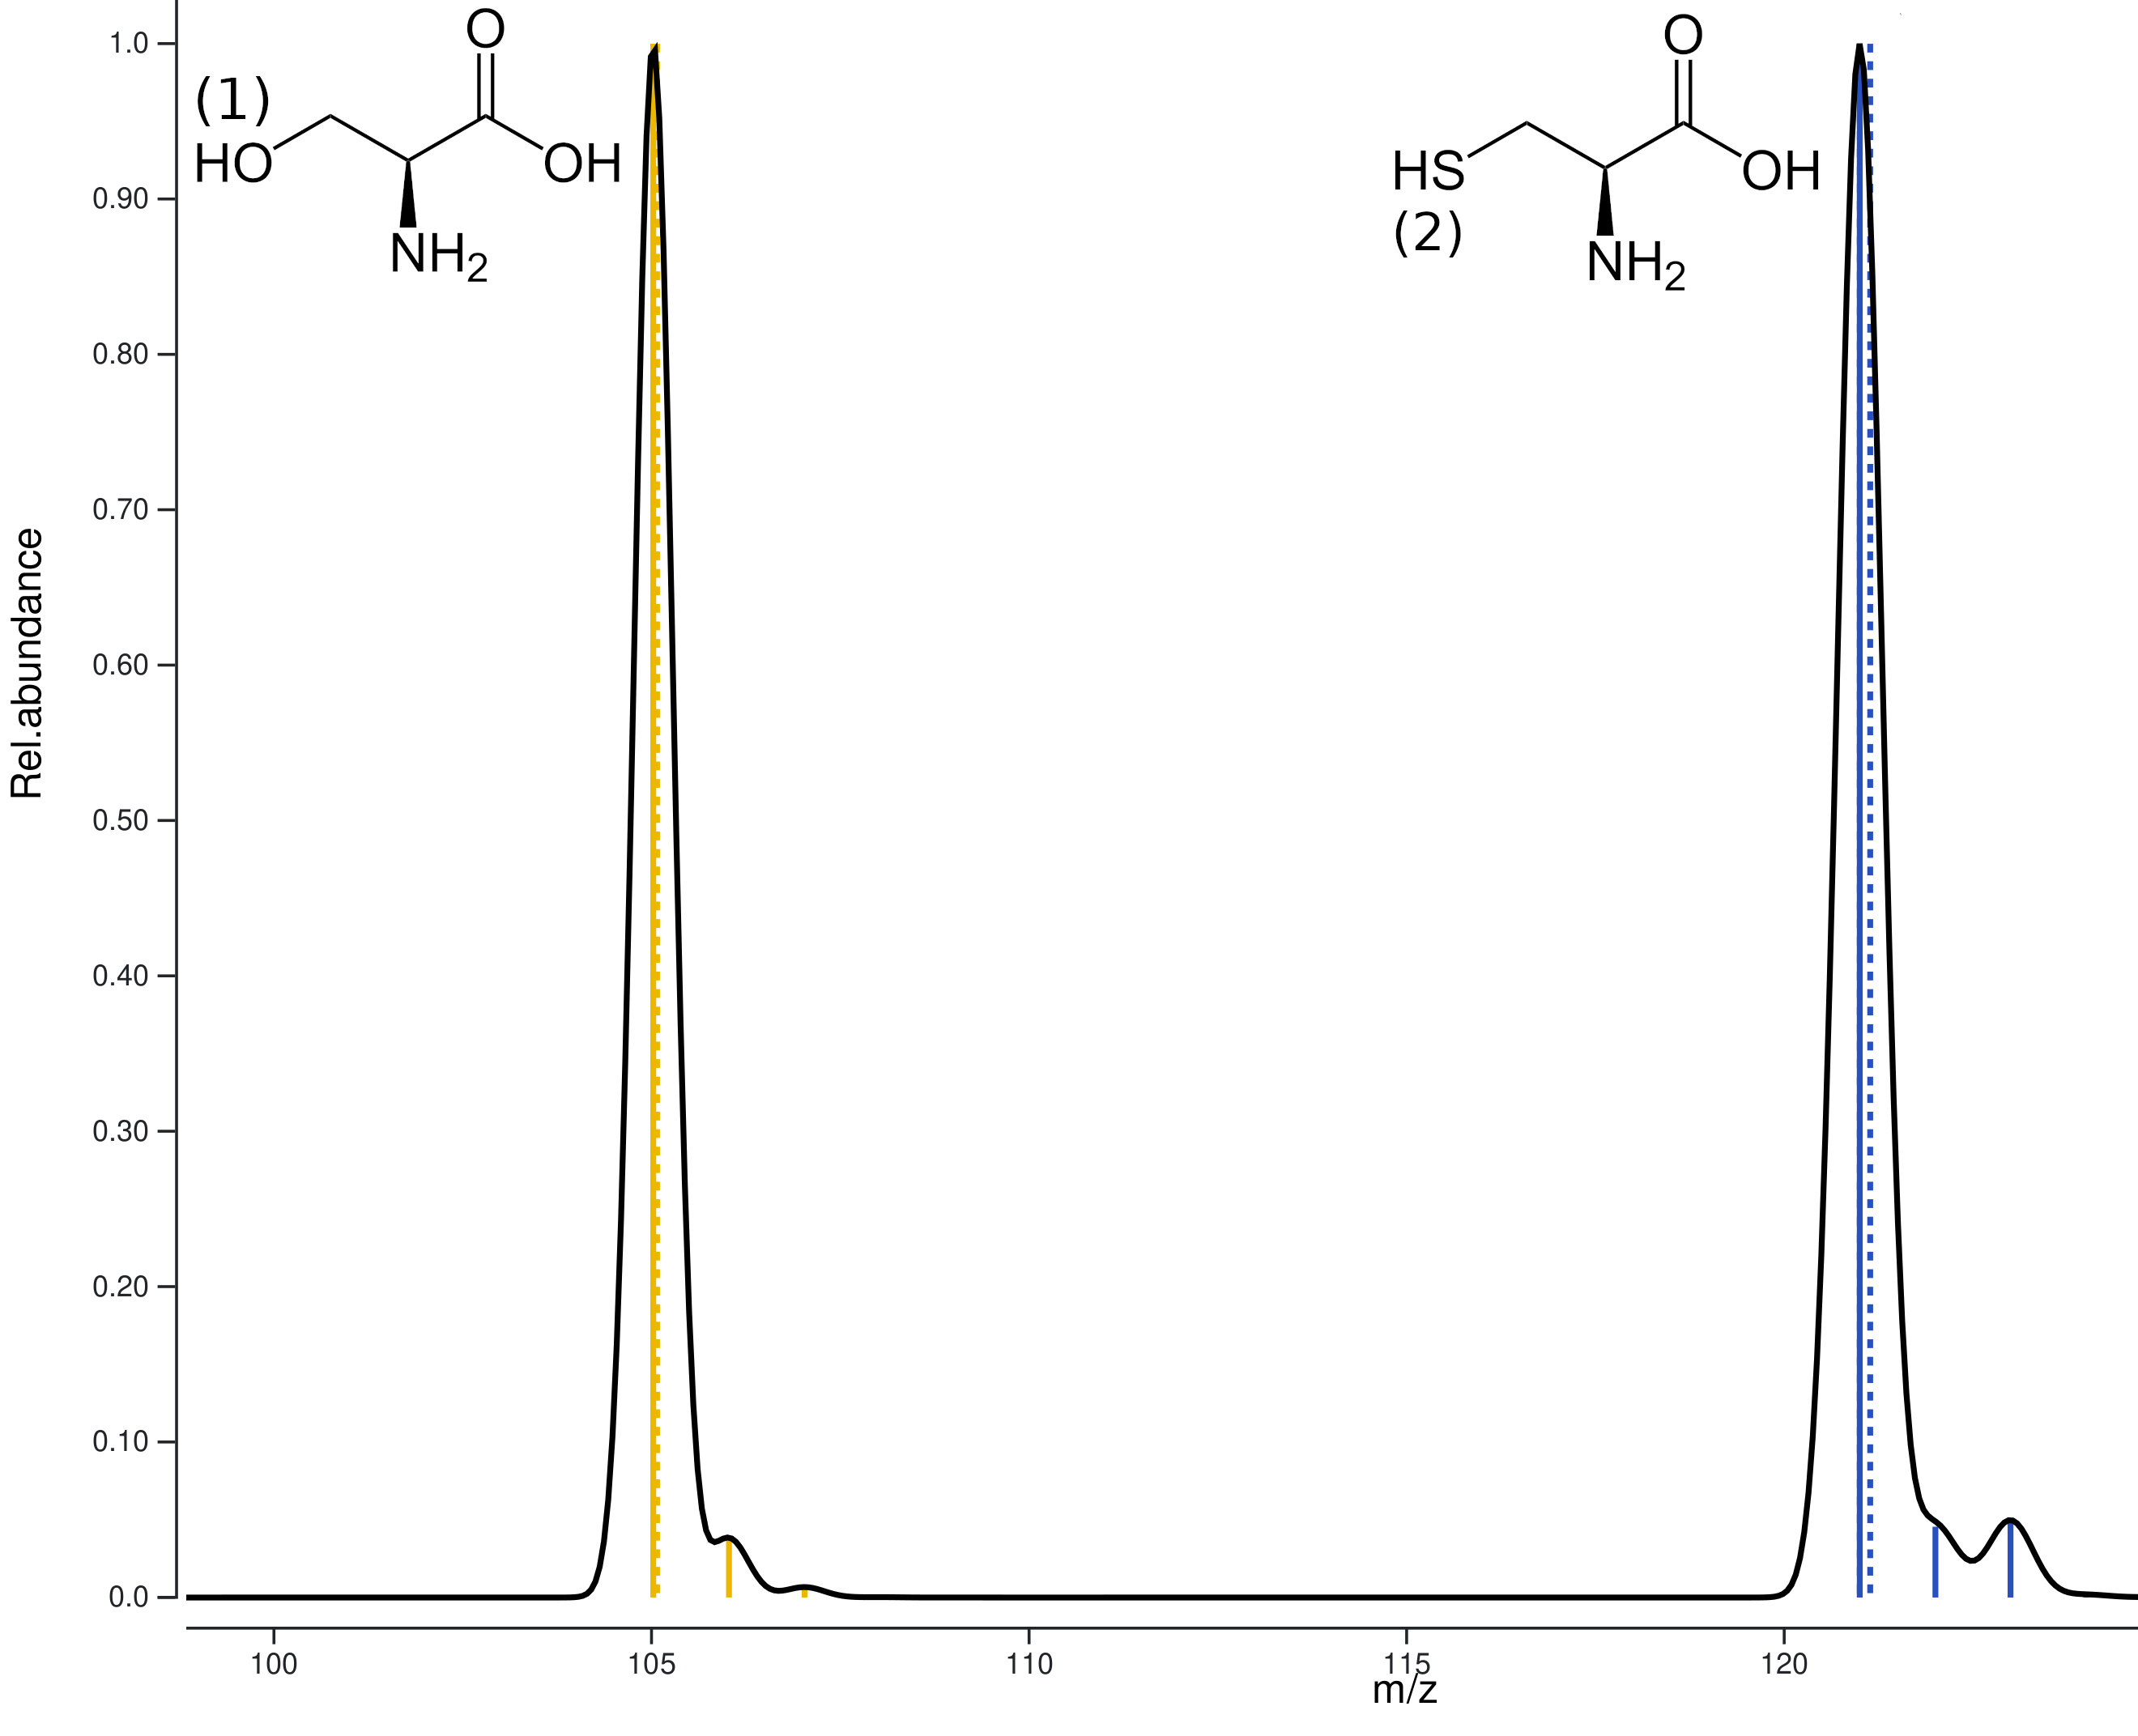
\includegraphics[width=0.75\textwidth]{./Resources/Simulated_Mass_Spectrum.png}
   \centering
   \caption{Computergeneriertes Massenspektrum von der Aminosäure \emph{Serin} (1) und \emph{Cystesin} (2). Peak von \emph{Serin} liegt bei 105; bei \emph{Systesin} um 121. y: relative Häufigkeit}
\end{figure}

Die Maxima werden \gerquot{Peaks} genannt und sind für eine Aminosäure an charakteristischer Position auf der $ x $-Achse. Obwohl sich die beiden Aminosäuren in der Abbildung \ref{fig:Sim_Mass_Spec} nur durch ein Atom unterscheiden (das linke Sauerstoffatom wurde durch ein Schwefelatom ersetzt) sind deren Massenspektren auf der $ x $-Achse weit voneinander entfernt und machen die beiden Aminosäuren dadurch sicher unterscheidbar.\\

Bei einzelnen Aminosäuren funktioniert die MS zuverlässig; bei Peptiden allerdings steht man vor dem Problem, dass das Massenspektrum unübersichtlicher wird und auch Peaks, die von Hintergrundrauschen stammen, schwerer herausgefiltert werden können. Abhilfe schafft hier die Tandem-Massenspektrometrie.

\subsection{Tandem-Massenspektrometrie (MS/MS)}\label{ss:Tandem_MS}
Bei der Tandem-Massenspektrometrie (MS/MS oder MS2) werden zwei MS Vorgänge hintereinander mit einer Probe durchgeführt. Die erste MS dient dazu Ionen aus einem bestimmten \massCharge Bereich auswählbar zu machen. Es entspricht also quasi einer Form der Filterung.

Vor der 2. MS werden die ausgewählten Reste einer Fragmentierung unterzogen. Bei einer Fragmentierung führt man Energie zu mit dem Ziel, dass die Ionen zerfallen und sog. Fragment-Ionen bilden. Diese Fragment-Ionen werden dann auf dem Massenspektrum nach der 2. MS sichtbar gemacht.

Fragment-Ionen sind kleiner als die ursprünglichen Ionen. So kann die 2. MS mit einer höheren Selektivität durchgeführt werden, welches Peaks durch Hintergrundrauschen verringert. Auch lassen sich Ionen besser identifizieren, die ein sehr ähnliches \massCharge-Verhältnis besitzen. Nach der 2. MS liegt eine Fülle an Fragment-Ionen-Peaks vor, aus denen sich die ursprünglichen Strukturinformationen ableiten lassen, da Ionen in spezifische Fragmente zerfallen \cite{Gross2013}. Zusammengefasst kann man sagen, dass das MS/MS Verfahren Ergebnisse höherer Güte erzeugt im Vergleich zur einfachen MS.

\section{De-Novo-Peptidsequenzierung mit \emph{pNovo+}}\label{s:pNovoPlusSeq}
Die \emph{pNovo+} Methode ist eine \gls{gls:DeNovo}, die mit einem \gls{gls:SpecGraph}en für die Auswertung der MS2-Spektren arbeitet und eine Erweiterung des \emph{pNovo} Verfahren darstellt \cite{pNovo}. Der Hauptansatz ist, dass zwei MS/MS Durchläufe mit jeweils verschiedenen Fragmentierungsmethoden\footnote{\emph{pNovo+} verwendet die higher energy
collisional dissociation (HCD) und die electron transfer dissociation (ETD) Fragmentierungsmethoden.} durchgeführt werden. Durch die Wahl einer anderen Fragmentierungsmethode ändert sich auch das MS2-Spektrum. Wenn nun Fragmentierungsmethoden verwendet werden, die möglichst komplementäre Spektren erzeugen, dann lässt sich durch das Zusammenführen der beiden MS2-Spektren die Qualität der Ergebnisse verbessern. Zum Beispiel lassen sich dadurch viele Peaks, die vom Hintergrundrauschen stammen, entfernen.

Für die Ermittlung der Sequenz eines Peptides wird zunächst ein Spektrums-Graph gebildet \dashAndSpace in Form eines DAG (directed acyclic graph). In diesem Graphen wird dann der längste Pfad bei gegebenen Start- und Endknoten berechnet. Die Reihenfolge der Knoten, die im längsten Pfad durchlaufen werden, stellt dann die Peptidsequenz dar.

\subsection{Vorverarbeitung der MS2-Spektren}\label{ss:Vorverarbeitung}
Bevor aus den MS2-Spektren der Spektrums-Graph gebildet werden kann, müssen die Daten vorverarbeitet werden. Für die Auswertung ist es von entscheidener Bedeutung, dass möglichst wenig Peaks verwendet werden, die vom Hintergrundrauschen stammen. Im weiteren Verlauf werden an einem exemplarischen MS2-Spektrum die Verarbeitungsschritte dargestellt.\\

Der erste Schritt ist das Verwenden des natürlichen Logarithmus der Intensitäten. Die Idee dabei ist, dass Hintergrundrauschen nicht überpriorisiert wird.

\begin{figure}[H]
   \centering
   \begin{minipage}[t]{.45\linewidth}
      \centering
      \begin{tikzpicture}[scale=\tikzScale, baseline=(current bounding box.center)]
         \draw [<->,thick] (0,\yAxisHeight) node (yaxis) [above] {\yAxisUnit}
         |- (\xAxisLength,0) node (xaxis) [right] {\xAxisUnit};
\draw[thick] (0.2, 0.0) -- (0.2, 2.3);
\draw[thick] (0.382, 0.0) -- (0.382, 1.7);
\draw[thick] (0.476, 0.0) -- (0.476, 2.7);
\draw[thick] (0.456, 0.0) -- (0.456, 1.8);
\draw[thick] (0.6859999999999999, 0.0) -- (0.6859999999999999, 2.7);
\draw[thick] (0.6839999999999999, 0.0) -- (0.6839999999999999, 1.8);
\draw[thick] (0.752, 0.0) -- (0.752, 1.1);
\draw[thick] (0.8200000000000001, 0.0) -- (0.8200000000000001, 2.2);
\draw[thick] (1.076, 0.0) -- (1.076, 1.5);
\draw[thick] (1.16, 0.0) -- (1.16, 1.9);
\draw[thick] (1.2120000000000002, 0.0) -- (1.2120000000000002, 2.0);
\draw[thick] (1.28, 0.0) -- (1.28, 1.9);
\draw[thick] (1.452, 0.0) -- (1.452, 1.3);
\draw[thick] (1.426, 0.0) -- (1.426, 1.9);
\draw[thick] (1.548, 0.0) -- (1.548, 1.9);
\draw[thick] (1.6740000000000002, 0.0) -- (1.6740000000000002, 1.5);
\draw[thick] (1.788, 0.0) -- (1.788, 2.5);
\draw[thick] (1.856, 0.0) -- (1.856, 2.3);
\draw[thick] (2.036, 0.0) -- (2.036, 1.7);
\draw[thick] (2.142, 0.0) -- (2.142, 1.6);
\draw[thick] (2.2520000000000002, 0.0) -- (2.2520000000000002, 2.0);
\draw[thick] (2.386, 0.0) -- (2.386, 1.6);
\draw[thick] (2.488, 0.0) -- (2.488, 2.9);
\draw[thick] (2.4739999999999998, 0.0) -- (2.4739999999999998, 2.7);
\draw[thick] (2.504, 0.0) -- (2.504, 2.0);
\draw[thick] (2.682, 0.0) -- (2.682, 2.0);
\draw[thick] (2.702, 0.0) -- (2.702, 2.5);
\draw[thick] (2.9259999999999997, 0.0) -- (2.9259999999999997, 2.8);
\draw[thick] (3.024, 0.0) -- (3.024, 2.4);
\draw[thick] (3.096, 0.0) -- (3.096, 1.8);
\draw[thick] (3.244, 0.0) -- (3.244, 2.6);
\draw[thick] (3.362, 0.0) -- (3.362, 1.9);
\draw[thick] (3.46, 0.0) -- (3.46, 2.3);
\draw[thick] (3.516, 0.0) -- (3.516, 1.1);
\draw[thick] (3.584, 0.0) -- (3.584, 1.8);
\draw[thick] (3.652, 0.0) -- (3.652, 2.0);
\draw[thick] (3.838, 0.0) -- (3.838, 1.5);
\draw[thick] (3.8819999999999997, 0.0) -- (3.8819999999999997, 2.6);
\draw[thick] (4.088, 0.0) -- (4.088, 2.6);
\draw[thick] (4.046, 0.0) -- (4.046, 1.1);
\draw[thick] (4.167999999999999, 0.0) -- (4.167999999999999, 2.0);
\draw[thick] (4.266, 0.0) -- (4.266, 2.4);
\draw[thick] (4.38, 0.0) -- (4.38, 1.1);
\draw[thick] (4.456, 0.0) -- (4.456, 2.2);
\draw[thick] (4.644, 0.0) -- (4.644, 2.6);
\draw[thick] (4.675999999999999, 0.0) -- (4.675999999999999, 2.5);
\draw[thick] (4.898000000000001, 0.0) -- (4.898000000000001, 1.2);
   \end{tikzpicture}%
   \end{minipage}%
   \textbf{$\rightarrow$} 
   \begin{minipage}[t]{.45\linewidth}
      \centering
      \begin{tikzpicture}[scale=\tikzScale, baseline=(current bounding box.center)]
      \draw [<->,thick] (0,\yAxisHeight) node (yaxis) [above] {\yAxisUnit}
      |- (\xAxisLength,0) node (xaxis) [right] {\xAxisUnit};
\draw[thick] (0.2, 0.0) -- (0.2, {ln(2.3)});
\draw[thick] (0.382, 0.0) -- (0.382, {ln(1.7)});
\draw[thick] (0.476, 0.0) -- (0.476, {ln(2.7)});
\draw[thick] (0.456, 0.0) -- (0.456, {ln(1.8)});
\draw[thick] (0.6859999999999999, 0.0) -- (0.6859999999999999, {ln(2.7)});
\draw[thick] (0.6839999999999999, 0.0) -- (0.6839999999999999, {ln(1.8)});
\draw[thick] (0.752, 0.0) -- (0.752, {ln(1.1)});
\draw[thick] (0.8200000000000001, 0.0) -- (0.8200000000000001, {ln(2.2)});
\draw[thick] (1.076, 0.0) -- (1.076, {ln(1.5)});
\draw[thick] (1.16, 0.0) -- (1.16, {ln(1.9)});
\draw[thick] (1.2120000000000002, 0.0) -- (1.2120000000000002, {ln(2.0)});
\draw[thick] (1.28, 0.0) -- (1.28, {ln(1.9)});
\draw[thick] (1.452, 0.0) -- (1.452, {ln(1.3)});
\draw[thick] (1.426, 0.0) -- (1.426, {ln(1.9)});
\draw[thick] (1.548, 0.0) -- (1.548, {ln(1.9)});
\draw[thick] (1.6740000000000002, 0.0) -- (1.6740000000000002, {ln(1.5)});
\draw[thick] (1.788, 0.0) -- (1.788, {ln(2.5)});
\draw[thick] (1.856, 0.0) -- (1.856, {ln(2.3)});
\draw[thick] (2.036, 0.0) -- (2.036, {ln(1.7)});
\draw[thick] (2.142, 0.0) -- (2.142, {ln(1.6)});
\draw[thick] (2.2520000000000002, 0.0) -- (2.2520000000000002, {ln(2.0)});
\draw[thick] (2.386, 0.0) -- (2.386, {ln(1.6)});
\draw[thick] (2.488, 0.0) -- (2.488, {ln(2.9)});
\draw[thick] (2.4739999999999998, 0.0) -- (2.4739999999999998, {ln(2.7)});
\draw[thick] (2.504, 0.0) -- (2.504, {ln(2.0)});
\draw[thick] (2.682, 0.0) -- (2.682, {ln(2.0)});
\draw[thick] (2.702, 0.0) -- (2.702, {ln(2.5)});
\draw[thick] (2.9259999999999997, 0.0) -- (2.9259999999999997, {ln(2.8)});
\draw[thick] (3.024, 0.0) -- (3.024, {ln(2.4)});
\draw[thick] (3.096, 0.0) -- (3.096, {ln(1.8)});
\draw[thick] (3.244, 0.0) -- (3.244, {ln(2.6)});
\draw[thick] (3.362, 0.0) -- (3.362, {ln(1.9)});
\draw[thick] (3.46, 0.0) -- (3.46, {ln(2.3)});
\draw[thick] (3.516, 0.0) -- (3.516, {ln(1.1)});
\draw[thick] (3.584, 0.0) -- (3.584, {ln(1.8)});
\draw[thick] (3.652, 0.0) -- (3.652, {ln(2.0)});
\draw[thick] (3.838, 0.0) -- (3.838, {ln(1.5)});
\draw[thick] (3.8819999999999997, 0.0) -- (3.8819999999999997, {ln(2.6)});
\draw[thick] (4.088, 0.0) -- (4.088, {ln(2.6)});
\draw[thick] (4.046, 0.0) -- (4.046, {ln(1.1)});
\draw[thick] (4.167999999999999, 0.0) -- (4.167999999999999, {ln(2.0)});
\draw[thick] (4.266, 0.0) -- (4.266, {ln(2.4)});
\draw[thick] (4.38, 0.0) -- (4.38, {ln(1.1)});
\draw[thick] (4.456, 0.0) -- (4.456, {ln(2.2)});
\draw[thick] (4.644, 0.0) -- (4.644, {ln(2.6)});
\draw[thick] (4.675999999999999, 0.0) -- (4.675999999999999, {ln(2.5)});
\draw[thick] (4.898000000000001, 0.0) -- (4.898000000000001, {ln(1.2)});
      \end{tikzpicture}
      \end{minipage}
      \caption{Anwendung des $ ln $ auf einem exemplarischen MS2-Spektrum.}
\end{figure}

Für das Verständnis des nächsten Schrittes muss man sich in Erinnerung rufen, dass eine gleiche Aminosäure keineswegs immer die gleiche Masse hat. Durch Isotope existiert eine gewisse \gerquot{Massenbandbreite} für ein und dieselbe Aminosäure. MS Systeme sind heute so genau, dass sie diese Differenzen erkennen. Dies hat den ungewollten Effekt, dass mehrere Peaks zu einer Aminosäure gehören können \cite{IsotopicDistributionMS}. Gleichzeitig können die \gerquot{Massenbandbreiten} zweier Aminosäuren sich überschneiden, sodass im ungünstigen Fall zwei Peaks kaum unterscheidbar nebeneinander liegen.\\

Eine Möglichkeit mit dieser Problematik umzugehen ist die Verwendung der monoisotopischen Masse. Die monoisotopische Masse ist die \gerquot{[...] exact mass of the most abundant naturally occurring stable isotope determined relative to the mass of 12 C, which is assigned the exact value of 12.0000.} \cite{MonoisotopicMass}. Ohne dabei jetzt tiefer ins Detail zu gehen kann man sagen, dass alle Peaks, deren Intensität mit einer möglichen monoisotopischen Masse übereinstimmen, auf jeden Fall einer Aminosäure entsprechen und (höchstwahrscheinlich)\footnote{Natürlich ist es möglich, dass das Rauschen zufällig einer monoisotopischen Masse entspricht. Die Wahrscheinlichkeit dafür ist allerdings sehr gering.} kein Hintergrundrauschen sind \cite{MassDefectMS}. Diese Peaks bekommen eine sogennante \emph{charge state}.\\

Der Algorithmus verwendet die \emph{charge state} Peaks als Ausganspunkte für weitere Berechnungen. Wenn die \massCharge Differenz zu einem anderen Peak einem Peptidfragment entspricht, dann stammt dieser Peak höchstwahrscheinlich von einem Fragment. Insgesamt werden damit die relevanten Peptidfragmente herausgeholt. Abbildung \ref{MonoisotopicMassFiltering} zeigt das Ergebnis nach den beiden zuvor genannten Schritten.

\begin{figure}[H]\label{MonoisotopicMassFiltering}
   \centering
   \begin{minipage}[t]{.45\linewidth}
      \centering
      \begin{tikzpicture}[scale=\tikzScale, baseline=(current bounding box.center)]
         \draw [<->,thick] (0,\yAxisHeight) node (yaxis) [above] {\yAxisUnit}
         |- (\xAxisLength,0) node (xaxis) [right] {\xAxisUnit};
\draw[thick] (0.2, 0.0) -- (0.2, {ln(2.3)});
\draw[color=blue!85!,opacity=.55,thick] (0.382, 0.0) -- (0.382, {ln(1.7)});
\draw[color=blue!85!,opacity=.55,thick] (0.476, 0.0) -- (0.476, {ln(2.7)});
\draw[color=magenta,thick] (0.456, 0.0) -- (0.456, {ln(1.8)});
\draw[color=blue!85!,opacity=.55,thick] (0.6859999999999999, 0.0) -- (0.6859999999999999, {ln(2.7)});
\draw[color=blue!85!,opacity=.55,thick] (0.6839999999999999, 0.0) -- (0.6839999999999999, {ln(1.8)});
\draw[thick] (0.752, 0.0) -- (0.752, {ln(1.1)});
\draw[thick] (0.8200000000000001, 0.0) -- (0.8200000000000001, {ln(2.2)});
\draw[thick] (1.076, 0.0) -- (1.076, {ln(1.5)});
\draw[thick] (1.16, 0.0) -- (1.16, {ln(1.9)});
\draw[thick] (1.2120000000000002, 0.0) -- (1.2120000000000002, {ln(2.0)});
\draw[thick] (1.28, 0.0) -- (1.28, {ln(1.9)});
\draw[color=blue!85!,opacity=.55,thick] (1.452, 0.0) -- (1.452, {ln(1.3)});
\draw[color=blue!85!,opacity=.55,thick] (1.426, 0.0) -- (1.426, {ln(1.9)});
\draw[color=magenta,thick] (1.548, 0.0) -- (1.548, {ln(1.9)});
\draw[color=blue!85!,opacity=.55,thick] (1.6740000000000002, 0.0) -- (1.6740000000000002, {ln(1.5)});
\draw[color=blue!85!,opacity=.55,thick] (1.788, 0.0) -- (1.788, {ln(2.5)});
\draw[thick] (1.856, 0.0) -- (1.856, {ln(2.3)});
\draw[thick] (2.036, 0.0) -- (2.036, {ln(1.7)});
\draw[thick] (2.142, 0.0) -- (2.142, {ln(1.6)});
\draw[thick] (2.2520000000000002, 0.0) -- (2.2520000000000002, {ln(2.0)});
\draw[thick] (2.386, 0.0) -- (2.386, {ln(1.6)});
\draw[color=blue!85!,opacity=.55,thick] (2.488, 0.0) -- (2.488, {ln(2.9)});
\draw[thick] (2.4739999999999998, 0.0) -- (2.4739999999999998, {ln(2.7)});
\draw[color=blue!85!,opacity=.55,thick] (2.504, 0.0) -- (2.504, {ln(2.0)});
\draw[color=magenta,thick] (2.682, 0.0) -- (2.682, {ln(2.0)});
\draw[color=blue!85!,opacity=.55,thick] (2.702, 0.0) -- (2.702, {ln(2.5)});
\draw[thick] (2.9259999999999997, 0.0) -- (2.9259999999999997, {ln(2.8)});
\draw[thick] (3.024, 0.0) -- (3.024, {ln(2.4)});
\draw[thick] (3.096, 0.0) -- (3.096, {ln(1.8)});
\draw[thick] (3.244, 0.0) -- (3.244, {ln(2.6)});
\draw[thick] (3.362, 0.0) -- (3.362, {ln(1.9)});
\draw[color=blue!85!,opacity=.55,thick] (3.46, 0.0) -- (3.46, {ln(2.3)});
\draw[color=blue!85!,opacity=.55,thick] (3.516, 0.0) -- (3.516, {ln(1.1)});
\draw[color=blue!85!,opacity=.55,thick] (3.584, 0.0) -- (3.584, {ln(1.8)});
\draw[color=magenta,thick] (3.652, 0.0) -- (3.652, {ln(2.0)});
\draw[color=blue!85!,opacity=.55,thick] (3.838, 0.0) -- (3.838, {ln(1.5)});
\draw[color=blue!85!,opacity=.55,thick] (3.8819999999999997, 0.0) -- (3.8819999999999997, {ln(2.6)});
\draw[thick] (4.088, 0.0) -- (4.088, {ln(2.6)});
\draw[thick] (4.046, 0.0) -- (4.046, {ln(1.1)});
\draw[thick] (4.167999999999999, 0.0) -- (4.167999999999999, {ln(2.0)});
\draw[thick] (4.266, 0.0) -- (4.266, {ln(2.4)});
\draw[color=blue!85!,opacity=.55,thick] (4.38, 0.0) -- (4.38, {ln(1.1)});
\draw[color=blue!85!,opacity=.55,thick] (4.456, 0.0) -- (4.456, {ln(2.2)});
\draw[color=magenta,thick] (4.644, 0.0) -- (4.644, {ln(2.6)});
\draw[color=blue!85!,opacity=.55,thick] (4.675999999999999, 0.0) -- (4.675999999999999, {ln(2.5)});
\draw[color=blue!85!,opacity=.55,thick] (4.898000000000001, 0.0) -- (4.898000000000001, {ln(1.2)});
   \end{tikzpicture}%
   \end{minipage}%
   \textbf{$\rightarrow$} 
   \begin{minipage}[t]{.45\linewidth}
      \centering
      \begin{tikzpicture}[scale=\tikzScale, baseline=(current bounding box.center)]
      \draw [<->,thick] (0,\yAxisHeight) node (yaxis) [above] {\yAxisUnit}
      |- (\xAxisLength,0) node (xaxis) [right] {\xAxisUnit};
\draw[color=blue!85!,opacity=.55,thick] (0.382, 0.0) -- (0.382, {ln(1.7)});
\draw[color=blue!85!,opacity=.55,thick] (0.476, 0.0) -- (0.476, {ln(2.7)});
\draw[color=magenta,thick] (0.456, 0.0) -- (0.456, {ln(1.8)});
\draw[color=blue!85!,opacity=.55,thick] (0.6859999999999999, 0.0) -- (0.6859999999999999, {ln(2.7)});
\draw[color=blue!85!,opacity=.55,thick] (0.6839999999999999, 0.0) -- (0.6839999999999999, {ln(1.8)});
\draw[color=blue!85!,opacity=.55,thick] (1.452, 0.0) -- (1.452, {ln(1.3)});
\draw[color=blue!85!,opacity=.55,thick] (1.426, 0.0) -- (1.426, {ln(1.9)});
\draw[color=magenta,thick] (1.548, 0.0) -- (1.548, {ln(1.9)});
\draw[color=blue!85!,opacity=.55,thick] (1.6740000000000002, 0.0) -- (1.6740000000000002, {ln(1.5)});
\draw[color=blue!85!,opacity=.55,thick] (1.788, 0.0) -- (1.788, {ln(2.5)});
\draw[color=blue!85!,opacity=.55,thick] (2.488, 0.0) -- (2.488, {ln(2.9)});
\draw[color=blue!85!,opacity=.55,thick] (2.504, 0.0) -- (2.504, {ln(2.0)});
\draw[color=magenta,thick] (2.682, 0.0) -- (2.682, {ln(2.0)});
\draw[color=blue!85!,opacity=.55,thick] (2.702, 0.0) -- (2.702, {ln(2.5)});
\draw[color=blue!85!,opacity=.55,thick] (3.46, 0.0) -- (3.46, {ln(2.3)});
\draw[color=blue!85!,opacity=.55,thick] (3.516, 0.0) -- (3.516, {ln(1.1)});
\draw[color=blue!85!,opacity=.55,thick] (3.584, 0.0) -- (3.584, {ln(1.8)});
\draw[color=magenta,thick] (3.652, 0.0) -- (3.652, {ln(2.0)});
\draw[color=blue!85!,opacity=.55,thick] (3.838, 0.0) -- (3.838, {ln(1.5)});
\draw[color=blue!85!,opacity=.55,thick] (3.8819999999999997, 0.0) -- (3.8819999999999997, {ln(2.6)});
\draw[color=blue!85!,opacity=.55,thick] (4.38, 0.0) -- (4.38, {ln(1.1)});
\draw[color=blue!85!,opacity=.55,thick] (4.456, 0.0) -- (4.456, {ln(2.2)});
\draw[color=magenta,thick] (4.644, 0.0) -- (4.644, {ln(2.6)});
\draw[color=blue!85!,opacity=.55,thick] (4.675999999999999, 0.0) -- (4.675999999999999, {ln(2.5)});
\draw[color=blue!85!,opacity=.55,thick] (4.898000000000001, 0.0) -- (4.898000000000001, {ln(1.2)});
      \end{tikzpicture}
      \end{minipage}
      \caption{Entfernen von Peaks, die keiner monoisotopischen Masse entsprechen oder benachbart mit einer Differenz von einem Fragment-Ion sind.}
\end{figure}

Tatsächlich ist die Verarbeitung an dieser Stelle noch etwas komplexer. So existieren auch noch sogenannte \emph{isotopic cluster}\footnote{Definition eines \emph{isotopic cluster} nach IUPAC: \gerquot{Group of peaks representing ions of the same elemental composition, but different isotopic compositions.} \cite[1556]{IUPACDefinitions}}, die gesondert verarbeitet werden. Für das grundsätzliche Prinzip ist dieses Detail allerdings weniger relevant.\\

Im letzten Vorberarbeitungsschritt werden Peaks aus einem irrelevanten \massCharge Bereich entfernt und naheliegende Peaks werden zusammengefasst, indem der Mittelwert sowol des \massCharge Wertes als auch der der Intensität besimmt wird. Üblicherweise liegt der Bereich für das Zusammenfassen bei $ +- 20 ppm $.

\begin{figure}[H]
   \centering
   \begin{minipage}[t]{.45\linewidth}
      \centering
      \begin{tikzpicture}[scale=\tikzScale, baseline=(current bounding box.center)]
         \draw [<->,thick] (0,\yAxisHeight) node (yaxis) [above] {\yAxisUnit}
         |- (\xAxisLength,0) node (xaxis) [right] {\xAxisUnit};
\draw[thick] (0.382, 0.0) -- (0.382, {ln(1.7)});
\draw[thick] (0.476, 0.0) -- (0.476, {ln(2.7)});
\draw[thick] (0.456, 0.0) -- (0.456, {ln(1.8)});
\draw[thick] (0.6859999999999999, 0.0) -- (0.6859999999999999, {ln(2.7)});
\draw[thick] (0.6839999999999999, 0.0) -- (0.6839999999999999, {ln(1.8)});
\draw[color=red,thick] (1.452, 0.0) -- (1.452, {ln(1.3)});
\draw[color=red,thick] (1.426, 0.0) -- (1.426, {ln(1.9)});
\draw[thick] (1.548, 0.0) -- (1.548, {ln(1.9)});
\draw[thick] (1.6740000000000002, 0.0) -- (1.6740000000000002, {ln(1.5)});
\draw[thick] (1.788, 0.0) -- (1.788, {ln(2.5)});
\draw[color=red,thick] (2.488, 0.0) -- (2.488, {ln(2.9)});
\draw[color=red,thick] (2.504, 0.0) -- (2.504, {ln(2.0)});
\draw[color=red,thick] (2.682, 0.0) -- (2.682, {ln(2.0)});
\draw[color=red,thick] (2.702, 0.0) -- (2.702, {ln(2.5)});
\draw[thick] (3.46, 0.0) -- (3.46, {ln(2.3)});
\draw[thick] (3.516, 0.0) -- (3.516, {ln(1.1)});
\draw[thick] (3.584, 0.0) -- (3.584, {ln(1.8)});
\draw[thick] (3.652, 0.0) -- (3.652, {ln(2.0)});
\draw[color=red,thick] (3.838, 0.0) -- (3.838, {ln(1.5)});
\draw[color=red,thick] (3.8819999999999997, 0.0) -- (3.8819999999999997, {ln(2.6)});
\draw[thick] (4.38, 0.0) -- (4.38, {ln(1.1)});
\draw[thick] (4.456, 0.0) -- (4.456, {ln(2.2)});
\draw[thick] (4.644, 0.0) -- (4.644, {ln(2.6)});
\draw[thick] (4.675999999999999, 0.0) -- (4.675999999999999, {ln(2.5)});
\draw[thick] (4.898000000000001, 0.0) -- (4.898000000000001, {ln(1.2)});

\fill[red!25!,opacity=.25] (0,0) rectangle (1,\yAxisHeight-\axisColorOffset);
         \fill[red!25!,opacity=.25] (\xAxisLength-1,0) rectangle (\xAxisLength-\axisColorOffset,\yAxisHeight-\axisColorOffset);
         \fill[green!25!,opacity=.25] (1,0) rectangle (\xAxisLength-1,\yAxisHeight-\axisColorOffset);
   \end{tikzpicture}%
   \end{minipage}%
   \textbf{$\rightarrow$} 
   \begin{minipage}[t]{.45\linewidth}
      \centering
      \begin{tikzpicture}[scale=\tikzScale, baseline=(current bounding box.center)]
      \draw [<->,thick] (0,\yAxisHeight) node (yaxis) [above] {\yAxisUnit}
      |- (\xAxisLength,0) node (xaxis) [right] {\xAxisUnit};
%\draw[color=red,thick] (1.452, 0.0) -- (1.452, {ln(1.3)});
%\draw[color=red,thick] (1.426, 0.0) -- (1.426, {ln(1.9)});
\draw[color=red,ultra thick] ({(1.452+1.426)/2}, 0.0) -- ({(1.452+1.426)/2}, {(ln(1.3)+ln(1.9))/2});

\draw[thick] (1.548, 0.0) -- (1.548, {ln(1.9)});
\draw[thick] (1.6740000000000002, 0.0) -- (1.6740000000000002, {ln(1.5)});
\draw[thick] (1.788, 0.0) -- (1.788, {ln(2.5)});

%\draw[color=red,thick] (2.488, 0.0) -- (2.488, {ln(2.9)});
%\draw[color=red,thick] (2.504, 0.0) -- (2.504, {ln(2.0)});
\draw[color=red,ultra thick] ({(2.488+2.504)/2}, 0.0) -- ({(2.488+2.504)/2}, {(ln(2.9)+ln(2.0))/2});

%\draw[color=red,thick] (2.682, 0.0) -- (2.682, {ln(2.0)});
%\draw[color=red,thick] (2.702, 0.0) -- (2.702, {ln(2.5)});
\draw[color=red,ultra thick] ({(2.682+2.702)/2}, 0.0) -- ({(2.682+2.702)/2}, {(ln(2.0+ln(2.5))/2});

\draw[thick] (3.46, 0.0) -- (3.46, {ln(2.3)});
\draw[thick] (3.516, 0.0) -- (3.516, {ln(1.1)});
\draw[thick] (3.584, 0.0) -- (3.584, {ln(1.8)});
\draw[thick] (3.652, 0.0) -- (3.652, {ln(2.0)});

%\draw[color=red,thick] (3.838, 0.0) -- (3.838, {ln(1.5)});
%\draw[color=red,thick] (3.8819999999999997, 0.0) -- (3.8819999999999997,{ln(2.6)});
\draw[color=red,ultra thick] ({(3.838+3.8819999999999997)/2}, 0.0) -- ({(3.838+3.8819999999999997)/2}, {(ln(1.5)+ln(2.6))/2});

\fill[red!25!,opacity=.25] (0,0) rectangle (1,\yAxisHeight-\axisColorOffset);
         \fill[red!25!,opacity=.25] (\xAxisLength-1,0) rectangle (\xAxisLength-\axisColorOffset,\yAxisHeight-\axisColorOffset);
         \fill[green!25!,opacity=.25] (1,0) rectangle (\xAxisLength-1,\yAxisHeight-\axisColorOffset);
      \end{tikzpicture}
      \end{minipage}
      \caption{Entfernen von Peaks aus einem irrelevanten \massCharge Bereich und zusammenfassen naheliegender Peaks. Rot markierte Peaks sind jene, die zusammengefasst werden.}
\end{figure}

\subsection{Bildung eines Spektrums-Graphen}\label{ss:BildungSpekGraph}
Der Spektrums-Graph wird aus einem vorverarbeiteten MS2-Spektrum (siehe Kapitel: \ref{ss:Vorverarbeitung}) gebildet. Im initialen Zustand werden die Peaks als Knoten interpretiert. Dazu kommt ein Start- und Endknoten. Jedem Knoten wird eine Masse zugeordet; im initialen Zustand bekommt der Startknoten die Masse 0 und der Endknoten die Masse des vorherigen Knotens minus der Masse des Wassers ($ 18,02 $). Die Masse der übrigen Knoten entsprechen ihren jeweils korrespondierenden \massCharge Wert. Die gerichteten Kanten werden zwischen einem Knotenpaar hinzugefügt, wenn die Differenz deren Masse gleich ist mit der Masse von ein oder zwei Aminosäuren.

\subsection{Identifikation der Aminosäuresequenz}
Der gebildete DAG kann mit klassischen Algorithmen, die den längsten Pfad suchen, durchlaufen werden. Bezogen auf die Graphentheorie entspricht die Ermittlung der Aminosäurensequenz dem Suchen eines bestimmten Pfades \dashAndSpace und nicht nach irgendeinem Pfad. Daher muss der Algorithmus mittels einer Breitensuche arbeiten, um alle möglichen Pfade zu bestimmen.

In aller Regel wird es mehrere Pfade geben. Bestimmte Sequenzen sind wahrscheinlicher als andere. So sind Pfade mit Kanten, die wegen der Massendifferenz von genau einer Aminosäure gebildet wurden, wahrscheinlicher \cite{pNovoPlus}. Alle Pfade bekommen mittels einer Scoring-Funktion einen Wert zugewiesen. Der Pfad mit dem höchsten Scoring-Wert ist wahrscheinlich das richtige Ergebnis. Die Scoring-Funktion berücksichtigt unter anderem wie viele Fragmente, die einer bestimmten Aminosäure zugeordet werden können, im MS2-Spektrum vorhanden sind \cite{pNovo}. Die Sequenz mit dem höchsten Scoring-Wert ist das Endergebnis.

\section{De-Novo-Peptidsequenzierung mit \emph{Open-pNovo}}\label{s:OpenpNovoSeq}
Bei Proteinen können posttranslationale Proteinmodifikationen (PTM) auftreten. PTMs sind Ereignisse, bei denen sich Änderungen im Protein einstellen \cite{Mann2003}; teilweise sind die Änderungen von einer Zelle erwünscht \dashAndSpace teilweise stammen sie aber auch zum Beispiel von unerwünschten Wechselwirkungen nebeneinanderliegenden Aminosäuren. Ein Teil dieser PTMs führen zu einer Änderung der Aminosäuresequenz. Dies ist für die \gls{gls:DeNovo} nicht weiter problematisch, da sowieso ohne eine Datenbank gearbeitet wird, sodass solche PTMs nicht einmal auffallen würden. Andere PTMs hingegen haben die Auswirkung, dass Stoffe gebildet werden, die nicht mehr zu der Gruppe der proteinogenen Aminosäuren gehören. Proteinogene Aminosäuren sind jene Aminosäuren, die für den Bau von Proteinen verwendet werden. Der Effekt ist also, dass Stoffe (oder deren Fragmente) bei einem Massenspektrum angezeigt werden, die kein Teil eines Peptids sein können. Bei der Sequenzierung von Peptidfragmenten muss dies daher berücksichtigt werden.
Wenn im weiteren Verlauf von PTMs gesprochen wird, dann sind solche gemeint, die für die \gls{gls:DeNovo} relevant sind.

Open-pNovo ist ein \gls{gls:DeNovo}sverfahren, welches auf pNovo+ Tool aufbaut und versucht die Problematik mit den PTMs zu lösen.

\subsection{PTMs im konstruierten DAG}
Die Konvertierung eines MS2-Spektrums läuft bis zum DAG analog ab wie in den Kapiteln \ref{ss:Vorverarbeitung} und \ref{ss:BildungSpekGraph} für pNovo+. Der Unterschied ist nun, dass es zwei Arten von Kanten gibt:

\begin{itemize}
   \item \gerquot{Normale} Kanten: Kanten, die gebildet werden, wie es bereits für \emph{pNovo+} gezeigt wurde. 
   \item \gerquot{Modifizierte} Kanten: Kanten, die zum Grahpen hinzugefügt werden, wenn die Massendifferenz zweier Knoten der Masse einer Aminosäure plus der Masse einer möglichen PTM-Änderung entspricht. 
\end{itemize}

Eine Liste aller PTMs in der Datenbank Unimod (sowohl relevante als auch nicht relevante) beinhaltet aktuell 1510 Einträge\footnote{Siehe: \url{https://www.ebi.ac.uk/ols/ontologies/unimod}} (Stand: 18.04.2022). Für die modifizierten Kanten gibt es insgesamt $ 1510 * 20 = 30200 $ mögliche Differenzen, wobei viele davon nicht relevante PTMs sind. Zum Vergleich: bei den normalen Kanten gibt es $ 20^2 = 400 $ mögliche Differenzen.

Die hohe Anzahl an Differenzen für modifizierte Kanten hat die Konsequenz, dass viele Knoten zufällig verbunden werden und dass dadurch die Genauigkeit der Ergebnisse abnimmt. Dieses Problem kann man durch eine geringere Liste an möglichen PTMs abfedern, allerdings mit einem Verlust  der Genauigkeit auf Seiten der PTMs. Es ist hier also eine Abwägung.

\subsection{Evaluierung von Open-pNovo}
Open-pNovo wurde sowohl auf drei realen als auch auf drei generierten Testdaten getestet. Tabelle \ref{tab:OpenPNovoResults} zeigt die Ergebnisse im Vergleich zu pNovo+ und zwei anderen Algorithmen. Die Datensätze enthielten die am häufigsten vorkommenden PTMs.

\begin{table}[H]
    \centering
    \begin{tabular}{l|c|c|c|c}
        \toprule
        \textbf{Testdatensätze} & \textbf{Open-pNovo+} & \textbf{pNovo+} & \textbf{PEAKS} & \textbf{Novor} \\
        \midrule
        Real (20259) & $76,3 \%$ & $68,5 \%$ & $65,8 \%$ & $39,9 \%$ \\
        Generiert (17877) & $77,8 \%$ & $0,6 \%$ & $0,5 \%$ & $0,2 \%$ \\
        \bottomrule
    \end{tabular}
    \newline
    \caption{Vergleich der durchschnittlichen richtigen \gls{gls:DeNovo} Peptidsequenzierungen von Open-pNovo und anderen Algorithmen \cite[650]{OpenPNovo}.}
    \label{tab:OpenPNovoResults}
\end{table}

Die enorm schlechten Ergebnisse der anderen Algorithmen bei den generierten Testdaten ist ein Nebeneffekt des Ziels bei der Testdatengenerierung. Denn diese wurden so ausgelegt, um die Grenzen von Open-pNovo+ zu ermitteln \cite[649]{OpenPNovo}. Eine Aussagekraft haben diese Ergebnisse also nicht. Allerdings auch bei realen Testdaten zeigt sich Open-pNovo als voll konkurrenzfähig gegenüber den anderen Algorithmen.

Noch besser zeigt sich Open-pNovo, wenn der Recall Wert betrachtet wird \dashAndSpace also die Anzahl an verschiedenen PSMs, die erkannt wurden. In diesem Fall ist der Abstand zu den anderen Algorithmen deutlich größer geworden.

\begin{table}[H]
    \centering
    \begin{tabular}{l|c|c|c|c}
        \toprule
        \textbf{Testdatensätze} & \textbf{Open-pNovo+} & \textbf{pNovo+} & \textbf{PEAKS} & \textbf{Novor} \\
        \midrule
        Real (5034) & $61,6 \%$ & $31,3 \%$ & $32,0 \%$ & $13,7 \%$ \\
        \bottomrule
    \end{tabular}
    \newline
    \caption{Vergleich der durchschnittlichen Recall Werte einer \gls{gls:DeNovo} Peptidsequenzierungen von Open-pNovo und anderen Algorithmen \cite[650]{OpenPNovo}.}
    \label{tab:OpenPNovoResultsRecall}
\end{table}

\subsection{Zusammenfassung}


% Die \gls{gls:DeNovo} nutzt die sogenannte \gls{gls:TMassSpek} für die Bestimmung der Peptidsequenz. Dabei wird die physikalische Eigenschaft ausgenutzt, dass jedes Atom bzw. jedes Molekül \dashAndSpace wenn es einer \gls{gls:Ionisation} unterzogen wurde \dashAndSpace ein charakteristisches \gls{gls:MassSpek} besitzt. Das \gls{gls:MassSpek} stellt also eine Art \gerquot{Fingerabdruck} eines Moleküls dar und macht dieses ermittelbar.

% U.U. eine Beispielgrafik eines Massenspektrums hinzufuegen ...

\subsubsection{\glsentrytext{gls:TMassSpek} bei größeren Molekülen}
Bei größeren Molekülen (wie einem Protein) führt die \gls{gls:Ionisation} dazu, dass das Molekül in kleinere spezifische Ionen zerfällt (sog. Fragmentierung). Die Fragmentierungsinformationen einer \gls{gls:DeNovo} sind meist unvollständig, da fehlende Daten bei einem Fragmentierungsschritt die Güte des Endergebnisses negativ beeinflusst. Dies wird insbesondere dann ein Problem, wenn unbekannte Änderungen in einer Peptidsequenz vorhanden sind.

Um dieses Problem zu verringern können unterschiedliche Techniken parallel eingesetzt werden, welche verschiedene Fragmente erzeugen und daher auch verschiedenartige \glspl{gls:MassSpek} zur Folge haben.\footnote{Konkret: Es wird sowohl das \gls{acr:HCD} als auch das \gls{acr:ETD} Verfahren angewendet.}

\subsection{Datenaufbereitung}
Typischerweise betrachtet man die sog. \gerquot{\glspl{gls:Peak}} in den \glspl{gls:MassSpek}. Jeder \gls{gls:Peak} stellt ein unterschiedliches Ion dar. Dazu kommen Messungenauigkeiten sowie Hintergrundrauschen. Durch die hohe Anzahl an möglichen Ionen kann nicht ohne weiteres differenziert werden, welcher der \glspl{gls:Peak} von welchen Ionen erzeugt wurden und welche nicht.

% Frage an Dominik: Ist hier eine einfache Auflistung an Techniken für die Datenaufbereitung besser?
Der Algorithmus für die Datenaufbereitung berechnet den natürlichen Logarithmus von den Intensitäten der \glspl{gls:Peak}, um Hintergrundrauschen und Messungenauigkeiten nicht überzupriorisieren. Zusätzlich dazu werden \glspl{gls:Peak}, die in einem Toleranzbereich nebeneinander liegen, zusammengefasst. Am Ende werden die \glspl{gls:Peak} entfernt, bei denen bekannt ist, dass es sich nicht um relevante Ionen handeln kann. (z.B. \glspl{gls:Peak} von Isotopen)

\begin{figure}[H]
   \centering
   \begin{minipage}[t]{.4\linewidth}
      \centering
      \begin{tikzpicture}[scale=\tikzScale, baseline=(current bounding box.center)]
         \draw [<->,thick] (0,2.75) node (yaxis) [above] {\yAxisUnit}
         |- (3,0) node (xaxis) [right] {\xAxisUnit};

         \draw[thick] (0.2,0) -- (0.2,1.1);
         \draw[thick] (0.3,0) -- (0.3,1.6);
         \draw[thick] (0.6,0) -- (0.6,1.7);
         \draw[thick] (0.8,0) -- (0.8,1.2);
         \draw[thick] (1.0,0) -- (1.0,1.1);

         \draw[color=red,thick] (1.2,0) -- (1.2,2.65);
         \draw[thick] (1.4,0) -- (1.4,1.4);
         \draw[thick] (1.6,0) -- (1.6,1.2);
         \draw[thick] (1.8,0) -- (1.8,1.3);
         \draw[thick] (2.0,0) -- (2.0,1.8);

         \draw[thick] (1.1,0) -- (1.1,2.0);
         \draw[color=red,thick] (0.35,0) -- (0.35,2.25);
         \draw[thick] (1.9,0) -- (1.9,1.4);
         \draw[color=red,thick] (2.2,0) -- (2.2,2.6);
         \draw[thick] (2.5,0) -- (2.5,1.25);

         \draw[thick] (2.7,0) -- (2.7,1.1);
         \foreach \x in {1,...,6}
         {
            \draw[thick] (1.2+\x*0.05,0) -- (1.2+\x*0.05,1.0+\x*0.15);
         }
      \end{tikzpicture}%
      % \subcaption{Exemplarische Rohdaten}
   \end{minipage}%
   \textbf{$\rightarrow$}
   \begin{minipage}[t]{.4\linewidth}
      \centering
      \begin{tikzpicture}[scale=\tikzScale, baseline=(current bounding box.center)]
         \draw [<->,thick] (0,2.75) node (yaxis) [above] {\yAxisUnit}
         |- (3,0) node (xaxis) [right] {\xAxisUnit};

         \draw[thick] (0.2,0) -- (0.2,{ln(1.1)});
         \draw[thick] (0.3,0) -- (0.3,{ln(1.6)});
         \draw[thick] (0.6,0) -- (0.6,{ln(1.7)});
         \draw[thick] (0.8,0) -- (0.8,{ln(1.2)});
         \draw[thick] (1.0,0) -- (1.0,{ln(1.1)});

         \draw[color=red,thick] (1.2,0) -- (1.2,{ln(2.65)});
         \draw[thick] (1.4,0) -- (1.4,{ln(1.4)});
         \draw[thick] (1.6,0) -- (1.6,{ln(1.2)});
         \draw[thick] (1.8,0) -- (1.8,{ln(1.3)});
         \draw[thick] (2.0,0) -- (2.0,{ln(1.8)});

         \draw[thick] (1.1,0) -- (1.1,{ln(2.0)});
         \draw[color=red,thick] (0.35,0) -- (0.35,{ln(2.25)});
         \draw[thick] (1.9,0) -- (1.9,{ln(1.4)});
         \draw[color=red,thick] (2.2,0) -- (2.2,{ln(2.6)});
         \draw[thick] (2.5,0) -- (2.5,{ln(1.25)});

         \draw[thick] (2.7,0) -- (2.7,{ln(1.1)});
         \foreach \x in {1,...,6}
         {%
            \draw[thick] (1.2+\x*0.05,0) -- (1.2+\x*0.05,{ln(1.0+\x*0.15)});
         }
      \end{tikzpicture}
      %\subcaption{Exemplarische Rohdaten}
   \end{minipage}
   \caption{Anwendung des $ln$ auf Rohdaten. Rote \glspl{gls:Peak} stellen hier exemplarisch fehlerhafte Daten dar, die nach dem $ln$ reduziert wurden.}
\end{figure}

\begin{figure}[H]
   \centering
   \begin{minipage}[t]{.4\linewidth}
      \centering
      \begin{tikzpicture}[scale=\tikzScale, baseline=(current bounding box.center)]
         \draw [<->,thick] (0,2.75) node (yaxis) [above] {\yAxisUnit}
         |- (3,0) node (xaxis) [right] {\xAxisUnit};

         \draw[thick] (0.2,0) -- (0.2,{ln(1.1)});
         \draw[thick] (0.3,0) -- (0.3,{ln(1.6)});
         \draw[thick] (0.6,0) -- (0.6,{ln(1.7)});
         \draw[thick] (0.8,0) -- (0.8,{ln(1.2)});
         \draw[thick] (1.0,0) -- (1.0,{ln(1.1)});

         \draw[thick] (1.2,0) -- (1.2,{ln(2.65)});
         \draw[thick] (1.4,0) -- (1.4,{ln(1.4)});
         \draw[thick] (1.6,0) -- (1.6,{ln(1.2)});
         \draw[thick] (1.8,0) -- (1.8,{ln(1.3)});
         \draw[thick] (2.0,0) -- (2.0,{ln(1.8)});

         \draw[thick] (1.1,0) -- (1.1,{ln(2.0)});
         \draw[thick] (0.35,0) -- (0.35,{ln(2.25)});
         \draw[thick] (1.9,0) -- (1.9,{ln(1.4)});
         \draw[thick] (2.2,0) -- (2.2,{ln(2.6)});
         \draw[thick] (2.5,0) -- (2.5,{ln(1.25)});

         \draw[thick] (2.7,0) -- (2.7,{ln(1.1)});
         \foreach \x in {1,...,6}
         {%
            \draw[color=red,thick] (1.2+\x*0.05,0) -- (1.2+\x*0.05,{ln(1.0+\x*0.15)});
         }

         \draw[dotted] (0.4,0) -- (0.4,2.75);
         \draw[dotted] (2.6,0) -- (2.6,2.75);
         \fill[red!25!,opacity=.25] (0,0) rectangle (0.4,2.75);
         \fill[red!25!,opacity=.25] (2.6,0) rectangle (3.0,2.75);
         \fill[green!25!,opacity=.25] (0.4,0) rectangle (2.6,2.75);
      \end{tikzpicture}
      %\subcaption{Exemplarische Rohdaten}
   \end{minipage}
   \textbf{$\rightarrow$}
   \begin{minipage}[t]{.4\linewidth}
      \centering
      \begin{tikzpicture}[scale=\tikzScale, baseline=(current bounding box.center)]
         \draw [<->,thick] (0,2.75) node (yaxis) [above] {\yAxisUnit}
         |- (3,0) node (xaxis) [right] {\xAxisUnit};

         \draw[thick] (0.6,0) -- (0.6,{ln(1.7)});
         \draw[thick] (0.8,0) -- (0.8,{ln(1.2)});
         \draw[thick] (1.0,0) -- (1.0,{ln(1.1)});

         \draw[thick] (1.2,0) -- (1.2,{ln(2.65)});
         %\draw[thick] (1.4,0) -- (1.4,{ln(1.4)});
         \draw[thick] (1.6,0) -- (1.6,{ln(1.2)});
         \draw[thick] (1.8,0) -- (1.8,{ln(1.3)});
         \draw[thick] (2.0,0) -- (2.0,{ln(1.8)});

         \draw[thick] (1.1,0) -- (1.1,{ln(2.0)});
         \draw[thick] (1.9,0) -- (1.9,{ln(1.4)});
         \draw[thick] (2.2,0) -- (2.2,{ln(2.6)});
         \draw[thick] (2.5,0) -- (2.5,{ln(1.25)});

         \draw[color=red,ultra thick] (1.2+1*0.05,0) -- (1.2+1*0.05,{ln(1.0+1*0.15)});
         \draw[color=red,ultra thick] (1.2+3*0.05,0) -- (1.2+3*0.05,{ln(1.0+3*0.15)});
         \draw[color=red,ultra thick] (1.2+5*0.05,0) -- (1.2+5*0.05,{ln(1.0+5*0.15)});

         \draw[dotted] (0.4,0) -- (0.4,2.75);
         \draw[dotted] (2.6,0) -- (2.6,2.75);
         \fill[red!25!,opacity=.25] (0,0) rectangle (0.4,2.75);
         \fill[red!25!,opacity=.25] (2.6,0) rectangle (3.0,2.75);
         \fill[green!25!,opacity=.25] (0.4,0) rectangle (2.6,2.75);
      \end{tikzpicture}
      %\subcaption{Exemplarische Rohdaten}
   \end{minipage}
   \caption{Entfernen von irrelevanten \glspl{gls:Peak} sowie zusammenfassen naheliegender \glspl{gls:Peak}. Hier symbolisieren die roten \glspl{gls:Peak} jene, die zusammengefasst werden.}
\end{figure}

% `\glsentrytext` funktioniert nicht für `\glspl`
\subsection{Konvertierung von \glspl{gls:MassSpek}}
Das Ziel der Konvertierung ist das Erzeugen eines \gls{gls:SpecGraph}en. Um von einem \gls{gls:MassSpek} zu einem \gls{gls:SpecGraph}en zu kommen, werden die \glspl{gls:Peak}, die nach der Datenaufbereitung (Siehe ...) übrig bleiben, als Knoten gewertet. Dazu kommt ein Start- und Endknoten. Jeder Knoten bekommt eine Gewichtung; diese Gewichtung entspricht der Stärke des \gls{gls:Peak}s.

\newcommand{\colorA}{white!30!green}
\newcommand{\colorB}{black!10!yellow}
\newcommand{\colorC}{white!40!red}
\newcommand{\colorD}{white!25!orange}
\newcommand{\colorE}{white!45!blue}
\newcommand{\colorF}{white!5!magenta}
\newcommand{\nodeFontSize}{\scriptsize}
\newcommand{\nodeScaleFactor}{100}
\newcommand{\round}[1]{\pgfmathprintnumber[precision=0]{#1}}
\newcommand{\rawA}{ln(1.7)}
\newcommand{\rawB}{ln(2.0)}
\newcommand{\rawC}{ln(2.65)}
\newcommand{\rawD}{ln(1.0+5*0.15)}
\newcommand{\rawE}{ln(1.85)}
\newcommand{\rawF}{ln(2.6)}
\newcommand{\valueA}{\pgfmathparse{int(\rawA*\nodeScaleFactor)}\pgfmathresult}
\newcommand{\valueB}{\pgfmathparse{int(\rawB*\nodeScaleFactor)}\pgfmathresult}
\newcommand{\valueC}{\pgfmathparse{int(\rawC*\nodeScaleFactor)}\pgfmathresult}
\newcommand{\valueD}{\pgfmathparse{int(\rawD*\nodeScaleFactor)}\pgfmathresult}
\newcommand{\valueE}{\pgfmathparse{int(\rawE*\nodeScaleFactor)}\pgfmathresult}
\newcommand{\valueF}{\pgfmathparse{int(\rawF*\nodeScaleFactor)}\pgfmathresult}

\begin{figure}[htb]
   \centering
      \begin{tikzpicture}[scale=\tikzScale*1.5, baseline=(current bounding box.center)]
         \draw [<->,thick] (0,2.75) node (yaxis) [above] {\yAxisUnit}
         |- (3,0) node (xaxis) [below] {\xAxisUnit};

         \draw[thick] (0.6,0) -- (0.6,{ln(1.7)}) node [right, rotate=90, color=\colorA] {\nodeFontSize\textbf{A} \valueA};
         \draw[thick] (0.8,0) -- (0.8,{ln(1.2)});
         \draw[thick] (1.0,0) -- (1.0,{ln(1.1)});

         \draw[thick] (1.2,0) -- (1.2,{ln(2.65)}) node [right, rotate=90,
         color=\colorC] {\nodeFontSize\textbf{C} \valueC};
         \draw[thick] (1.4,0) -- (1.4,{ln(1.4)});
         \draw[thick] (1.6,0) -- (1.6,{ln(1.2)});
         \draw[thick] (1.8,0) -- (1.8,{ln(1.3)});
         \draw[thick] (2.0,0) -- (2.0,{ln(1.8)}) node [right, rotate=90, color=\colorE] {\nodeFontSize\textbf{E} \valueE};

         \draw[thick] (1.025,0) -- (1.025,{ln(2.0)}) node [right, rotate=90, color=\colorB] {\nodeFontSize\textbf{B} \valueB};
         \draw[thick] (1.9,0) -- (1.9,{ln(1.4)});
         \draw[thick] (2.2,0) -- (2.2,{ln(2.6)}) node [right, rotate=90, color=\colorF] {\nodeFontSize\textbf{F} \valueF};
         \draw[thick] (2.5,0) -- (2.5,{ln(1.25)});

         \draw[thick] (1.2+1*0.05,0) -- (1.2+1*0.05,{ln(1.0+1*0.15)});
         \draw[thick] (1.2+3*0.05,0) -- (1.2+3*0.05,{ln(1.0+3*0.15)});
         \draw[thick] (1.2+5*0.05,0) -- (1.2+5*0.05,{ln(1.0+5*0.15)}) node [right, rotate=90, color=\colorD] {\nodeFontSize\textbf{D} \valueD};
      \end{tikzpicture}
      \caption{Ausgewählte \glspl{gls:Peak} mit einem exemplarischen x Wert.}
\end{figure}

\newcommand{\modVal}{4}

Gerichtete Kanten zwischen den Knoten werden ausgebildet, wenn diese eine Differenz von genau einer oder zwei Aminosäurereste\footnote{Da eine Aminosäure vielerlei an Reste besitzen kann, ergeben sich mehr als 40 Differenzen, die diese Bedingung erfüllen.} besitzen. Der Einfachheit halber wird im folgenden eine Kante ausgebildet, wenn die Differenz genau \textbf{\modVal} \space beträgt.

% Um einzele Knotennamen einzufärben: \textcolor{\colorA}{A}
\newcommand{\findRaw}[1]{\csname raw#1\endcsname}
\newcommand{\findValue}[1]{\csname value#1\endcsname}
\newcommand{\findColor}[1]{\csname color#1\endcsname}
\newcommand{\cmark}{\ding{51}}
\newcommand{\xmark}{\ding{55}}
\newcommand{\tableRow}[2]
{%
   % Welche Zeile soll farblich hinterlegt werden ?
   \pgfmathparse{Mod(abs(int(\findRaw{#1}*\nodeScaleFactor) - int(\findRaw{#2}*\nodeScaleFactor)),\modVal)}
   \pgfmathtruncatemacro\myresult{\pgfmathresult==0.0?1:0}
   %\ifthenelse{\myresult=1}{A}{B}
   \ifnum\myresult=1 A \else B \fi

   (#1,#2) &
   \findValue{#1} &
   \findValue{#2} &
   \pgfmathparse{abs(int(\findRaw{#1}*\nodeScaleFactor) - int(\findRaw{#2}*\nodeScaleFactor))}\round{\pgfmathresult} &

   % Hilfreiche Infos für das Erstellen von Ausdrücken: https://tikz.dev/math-parsing
   \pgfmathparse{Mod(abs(int(\findRaw{#1}*\nodeScaleFactor) - int(\findRaw{#2}*\nodeScaleFactor)),\modVal)}
   % https://www.reddit.com/r/LaTeX/comments/57ck5p/tikz_which_conditionals_to_use_to_compare_numbers/
   \pgfmathtruncatemacro\myresult{\pgfmathresult==0.0?1:0}
   \round{\pgfmathresult}
   \ifthenelse{\myresult=1}{\cmark}{\xmark}
   \\
}
% Hilfestellung: https://tex.stackexchange.com/questions/604496/how-to-generate-beautiful-tables-in-latex
\begin{table}[H]
    \centering
    \begin{tabular}{lllcc}
        \toprule
        \thead{\textbf{$\mathbf{(u,v)}$}} & \thead{$\mathbf{u}$} & \thead{$\mathbf{v}$} & \thead{$\mathbf{\Delta(u,v)}$} & \thead{$\Delta(u,v)\bmod\modVal$}\\
        \midrule
        \tableRow{A}{B}
        \tableRow{A}{C}
        \tableRow{A}{D}
        \tableRow{A}{E}
        \tableRow{A}{F}
        \tableRow{B}{C}
        \tableRow{B}{D}
        \tableRow{B}{E}
        \tableRow{B}{F}
        \tableRow{C}{D}
        \tableRow{C}{E}
        \tableRow{C}{F}
        \tableRow{D}{E}
        \tableRow{D}{F}
        \tableRow{E}{F}
        \bottomrule
    \end{tabular}
    \caption{Bestimmung der Kanten}
\end{table}

Darstellung der Daten als gewichteter, gerichteter azyklischer Graph. Zusätzlich benötigt der Graph noch separate Start- und Zielknoten; diese sind für die späteren Berechnungen unerlässlich.

\newcommand{\printVertices}[2]%
{%
   \Vertex[x=-8,y=0]{Start}
   \Vertex[x=8,y=0]{End}
   \foreach \x [count=\xi] in {#1}
   {%
      \foreach \y [count=\yi] in {#2}
      {%
         \ifthenelse{\xi=\yi}{
         \tikzstyle{VertexStyle}=[shape=circle,fill=\y,draw=black,line width=0.75pt]
         \Vertex[x=-7+\xi*2,y=0]{\x}}{\break}
      }
   }
}
% https://tex.stackexchange.com/questions/245448/adjusting-edge-and-vertex-label
\begin{figure}[htb]
   \centering
   \begin{tikzpicture}[scale=0.75,transform shape]
      \tikzstyle{VertexStyle}=[shape=circle,fill=white,draw=black,line width=1pt]

      \printVertices{A,B,C,D,E,F}{\colorA, \colorB, \colorC, \colorD, \colorE, \colorF}

      \tikzstyle{LabelStyle}=[fill=white, sloped]
      \tikzstyle{EdgeStyle}=[bend left, post]
      \Edge[label=$0$](Start)(A)
      \Edge[label=$0$](F)(End)
      \tikzstyle{EdgeStyle}=[bend right, post]
      \Edge[label=$16$](A)(B)
      \tikzstyle{EdgeStyle}=[bend left, post]
      \Edge[label=$44$](A)(C)
      \Edge[label=$8$](A)(E)
      \tikzstyle{EdgeStyle}=[bend right, post]
      \Edge[label=$28$](B)(C)
      \Edge[label=$8$](B)(E)
      \Edge[label=$36$](C)(E)
      \tikzstyle{EdgeStyle}=[bend left, post]
      \Edge[label=$40$](D)(F)
   \end{tikzpicture}
   \caption{Erzeugter DAG}
\end{figure}

Bereits an diesem Minimalbeispiel ist zu erkennen, dass die gebildeten Knoten in einem \glspl{gls:SpecGraph} nur wenige ausgehende Kanten besitzen. Dies ist nicht dem Beispiel geschuldet sondern ist tatsächlich auch in der Praxis der Regelfall. Dies ist eine hilfreiche Beobachtung für die Datenauswertung (siehe Abschnitt~\ref{Datenauswertung} \gerquot{\titleref{Datenauswertung}}).


\subsection{Datenauswertung}\label{Datenauswertung}
Um nun aus dem Graphen die Peptidsequenz zu gewinnen müssen alle längsten Pfade im DAG gefunden werden. Da die Kanten gewichtet sind, kann es durchaus mehrere längste Pfade geben. Gleichwohl es Algorithmen für das Problem des längsten Pfades in einem Graphen gibt, handelt es sich hierbei um ein $NP$-schweres Problem. Es existiert also (wahrscheinlich) kein effizienter Algorithmus. Erschwerend kommt hinzu, dass der Graph nicht zwingend ein zusammenhängender Graph sein muss \dashAndSpace auch wenn dies meist der Fall ist. Der Graph muss daher vor Berechnungsbeginn auf diese Eigenschaft hin überprüft werden.

Im Falle der \glspl{gls:SpecGraph} existiert die Eigenschaft, dass solche Graphen meist eine geringe Dichte an Kanten aufweisen. Dies hat den positiven Effekt, dass die Anzahl an überhaupt möglichen längsten Pfaden recht gering ist. Zusätzlich dazu kann die Warteschlange, die in den longest Path DAG Algorithmen verwendet werden, angepasst werden. Da die Gewichtung der Kanten als eine Art \gerquot{Wahrscheinlichkeit}, dass die nächste Kante die reale Peptidsequenz darstellt, interpretiert werden kann, kann eine priorisierte Warteschlange verwendet werden, die die Laufzeit ebenfalls verbessert. In Summe führen diese Eigenschaften der \glspl{gls:SpecGraph} dazu, dass das längste Pfade Problem in solchen Fällen auf die Laufzeit $\mathcal{O}(abs(E) + log(d))$ reduziert werden kann.\\

Zusammengefasst: Es wird versucht die speziellen Eigenschaften der Graphen auszunutzen, um die Laufzeit zu verbessern.


\section{Ergebnisse/Evaluierung}
Im folgenden Kapitel werden die Probleme, die in der Praxis bei der Verwendung des Verfahrens auftreten, erläutert und mögliche Lösungsansätze aufgezeigt.

\subsection{Probleme in der Praxis}
\subsubsection{Qualität der Messwerte}
Obwohl eine Datenaufbereitung stattfindet, ist das Verfahren bei der Verwendung von \glspl{gls:SpecGraph} stark auf die Genauigkeit der Messwerte angewiesen. Zwar sind durch technische Fortschritte bei der \gls{gls:TMassSpek} die Daten hochwertiger geworden; dennoch gestaltet sich das Sequenzieren von unbekannten Peptidsequenzen als schwierig. Mit heutigen Gerätschaften lassen sich bei der Verwendung des genannten Verfahrens bis zu 13 Peptide mit einer durchschnittlichen Genauigkeit von 94\% ermitteln. Danach nimmt diese sprunghaft ab. Für brauchbare Ergebnisse wird \dashAndSpace je nach Literatur \dashAndSpace eine Trefferquote von 90-95\% vorausgesetzt.
\subsubsection{Fehlende Betrachtung der \glsentrytext{gls:StereoIsomerie}}\label{FehlendeStereoInfos}
Das komplette Verfahren basiert auf das Masse-Ladungs-Verhältnis, sodass Stereoinformationen schlicht nicht ermittelt werden können. Es kann zwar mithilfe einer energetischen Betrachtung bestimmt werden welche \glspl{gls:StereoIsomer} in welchen Verhältnis auftreten (müssten). Dabei handelt es sich allerdings lediglich um eine grobe Abschätzung.
\subsubsection{Identifikation der Aminosäuren über Massendifferenz}
Die Grundidee bei der Identifikation von Aminosäuren ist die Betrachtung der Massendifferenzen zwischen zwei \glspl{gls:Peak}. Zwar liefert dieser Ansatz häufig passende Ergebnisse. Dennoch ist solch eine Differenz nicht in der Lage jede Aminosäure immer eindeutig zu identifizieren, da bestimmte Kombinationen (fast) gleiche Differenzen besitzen. Der Algorithmus, der die Gewichtungen bestimmt, arbeitet nur mit ganzzahligen Werten. Dadurch gehen leichte Unterschiede, die durch die Isotope (insb. die des Kohlenstoffes) begründet sind, meist durch die Float Integer Konvertierung verloren.

\subsection{Lösungsansätze}
\subsubsection{Verbesserung der Ergebnisse durch Machine Learning}
Bei der Sequenzierung werden ab einer gewissen Länge unweigerlich Fehler eintreten.\cite[S.621,Figure 5]{pNovoPlus} Dadurch, dass nicht jede Peptidsequenz gleich wahrscheinlich ist\footnote{Dies ist u.a. dadurch begründet, dass die Reste der Aminosäuren sich gegenseitig beeinflussen (können), sodass bestimmte Sequenzen energetisch ungünstig sind und lediglich vermindert auftreten.}, können mittels Machine Learning grundsätzlich die Ergebnisse verbessert werden. insbesondere dann, wenn die ermittelte Differenz keinen eindeutigen Rückschluss auf die Aminosäure zulässt.

\section{Zusammenfassung}
Im letzten Kapitel werden die ungelösten Probleme genannt und erklärt warum diese eine Relevanz für die Praxis haben. Am Ende findet eine kritische Betrachtung des Verfahrens im allgemeinen statt.

\subsection{Ungelöste Probleme}
Wie bereits in \ref{FehlendeStereoInfos} erwähnt, kann das Verfahren designbedingt keine Stereoinformationen ermitteln. Daher ist es in diesem Fall besonders wichtig abzuschätzen, ob das Fehlen dieser Informationen tatsächlich eine Relevanz hat. Wenn nur die Peptidsequenz betrachtet werden soll, dann stellt dies kein Problem dar. Aber sobald jedweige Abschätzungen anhand der ermittelten Sequenz stattfinden soll, dann kann das Fehlen jener Informationen zu massiven Fehlern führen.\\

Wenn für die Verbesserung der Ergebnisse Machine Learning in Betracht kommt, dann muss dabei berücksichtigt werden, dass dadurch unter Umständen einer der großen Vorteile der \gls{gls:DeNovo} verloren geht \dashAndSpace und zwar dass keine Vorinformationen für die Sequenzierung notwendig sind. Hierbei kommt es auf den konkreten Anwendungsfall an, ob das Verlieren dieser Eigenschaft eine Bedeutung besitzt.

\subsection{Kritische Betrachtung}
Die \gls{gls:DeNovo} mit der Unterstützung von \glspl{gls:SpecGraph} stellt eine Möglichkeit dar Polypeptide mit bis zu einer Länge von etwa 12 Peptiden ausreichend zuverlässig zu bestimmen. Die Autoren des Papers \cite{OpenPNovo} haben die Software frei zur Verfügung gestellt, sodass sie in jedem Fall ein Blick wert ist.
Gegenüber anderen Ansätzen ist das Verfahren zwar konkurrenzfähig, allerdings nicht immer die beste Wahl \cite[650]{OpenPNovo}. Die Grundidee mittels der Massendifferenz auf die Aminosäuren zu schließen wird nie fehlerfrei sein, sodass dieses Verfahren weniger die bereits vorhandenen Systeme ersetzten kann, sondern eher ein weiteres Werkzeug für die \gls{gls:DeNovo} darstellt.

\begingroup
\setlength{\emergencystretch}{.5em}
\printbibliography
\endgroup

\end{document}
%%%%% %%%%% %%%%% %%%%% %%%%% \end{document} %%%%% %%%%% %%%%% %%%%% %%%%%


\newcommand{\gerquot}[1]{\glqq#1\grqq}
\newcommand{\dashAndSpace}{\textendash \space}
\newcommand{\dashAndSpaceSeq}[1]{\dashAndSpace#1 \dashAndSpace}
\newcommand{\tikzScale}{1.0}
\newcommand{\massCharge}{$ m/z $ }
\newcommand{\xAxisUnit}{\massCharge}
\newcommand{\yAxisUnit}{$y$}
\newcommand{\yAxisHeight}{3}
\newcommand{\xAxisLength}{5}
\newcommand{\axisColorOffset}{0.15}

\renewcommand{\floatpagefraction}{0.8}
% Workaround um die Überschrift des Glossars anzupassen
% Siehe: https://tex.stackexchange.com/questions/426390/how-can-i-rename-the-header-titles-of-the-glossary
\addto\captionsngerman
{%
    \renewcommand*{\glossaryname}{Begriffserklärungen}%
}
  


%%%%% %%%%% %%%%% %%%%% %%%%% \begin{document} %%%%% %%%%% %%%%% %%%%% %%%%%
\begin{document}

\maketitle

\section{Einleitung}\label{s:Einleitung}
\subsection{Biomedizinische Fragestellung}
Peptide sind organische Verbindungen von miteinander verknüpften Aminosäuren. Bei der Sequenzierung von Peptiden versucht man die Aminosäuresequenz \dashAndSpaceSeq{also die Abfolge an vorhandenen Aminosäuren} zu bestimmen. Das Wissen über die Aminosäuresequenz ist von großer Bedeutung für den Forschungsbereich der Proteomik. Die Proteomik beschäftigt sich mit der Erforschung von Proteinen. Dies beinhaltet unter anderem auch die Analyse von Enzymen.

Da es 20 verschiedene Aminosäuren gibt \cite{rudat2021alanins}, die weitesgehend beliebig miteinander kombiniert werden können, existiert eine stark wachsende Anzahl an möglichen Variationen (oder Kombinationen(!)). Die Regeln der Kombinatik liefert uns hierfür die Formel $ f(x)=20^x $ wobei $ x $ hier die Anzahl an Aminosäuren ist. Es ist direkt erkennbar, dass selbst bei einer geringen Peptidlänge die Anzahl an möglichen Sequenzen eine Größenordnung erreicht, die von Computersystemen nicht mehr verarbeitet werden kann. Zum Vergleich: Proteine können aus wenigen Hundert bis hin zu aus mehreren Zehntausend Aminosäuren bestehen. Die Frage, die sich hier stellt: \emph{Ist es zumindest für kurze Peptide mögich diese sicher zu sequenzieren?}

\subsection{Methoden der Aminosäuresequenzierung}
Das Ziel der verschiedenen Sequenzierungsverfahren ist eine möglichst exakte Bestimmung der Aminosäuresequenz. Alle Sequenzierungsverfahren arbeiten mit der Massenspektrometrie (MS). Dabei handelt es sich um ein Verfahren, welches chemische Verbindungen identifizieren kann (eine genauere Erklärung folgt in Kapitel \ref{s:MS}). Viele Analysen arbeiten mit dem Ansatz, dass die Ergebnisse einer MS \dashAndSpaceSeq{genannt wird es Massenspektrum} mit einer Datenbank verglichen werden. Wenn die chemische Verbindung bereits einmal indentifiziert wurde, dann wird sich ein Eintrag in der Datenbank finden lassen.

Die hier vorgestellten Methoden \emph{pNovo+} und \emph{Open-pNovo} gehören zur Gruppe der \gls{gls:DeNovo}en. Im Gegensatz zu anderen Verfahren werden hierbei keinerlei Daten aus Datenbanken verwendet. Stattdessen findet eine Tandem-Massenspektrometrie Anwendung. Bei dieser Form der MS werden zwei MS Durchgänge hintereinander durchgeführt, wobei nach dem ersten Vorgang ein Teil der Probe isoliert wird und vor der 2. MS \gerquot{fragmentiert} wird (hierzu eine Beschreibung in Kapitel \ref{ss:Tandem_MS} mit mehr Details). Die \gls{gls:DeNovo} hat den bedeutsamen Vorteil, dass auch Peptide sequenziert werden können zu denen es keine oder nur unvollständige Informationen gibt.

% Im ersten Kapitel findet zu Beginn eine Erklärung der wichtigsten Begriffe und Abkürzungen statt. Dazu wird eine Themenabgrenzung durchgeführt sowie die Ausgangssituation beschrieben.

% \printnoidxglossaries

%\subsection{Themenabgrenzung}
%Folgende Aspekte sind Bestandteil dieser Ausarbeitung:
%\begin{itemize}
%   \item Was ist die \gls{gls:DeNovo}?
%   \item Was erhofft man sich von dieser Technologie?
%   \item Welche Probleme liegen vor, die von der Seite der Informatik %gelöst / verbessert werden können?
%   \item Inwiefern spielen die Spektrums-Graphen dabei eine Rolle?
%\end{itemize}


% In diesem Abschnitt werden die relevanten Herangehensweisen sowohl für die Datengewinnung als auch für deren Auswertung erklärt.

\section{Massenspektrometrie (MS)}\label{s:MS}
Wie bereits in Kapitel \ref{s:Einleitung} erwähnt, wird die MS verwendet, um chemische Strukturen zu identifizieren. Moderne Ansätze der MS wurden zu Beginn des 20. Jahrhunderts entwickelt \cite{griffiths2008brief}. Seitdem gab es etliche Erweiterungen; das Grundprinzip ist dennoch immer gleich geblieben. Grob vereinfacht besteht eine MS aus folgenden vier Schritten:

\begin{itemize}
   \item \textbf{Ionisation}: Die Moleküle in der Probe bekommen eine positive oder negativ Ladung
   \item \textbf{Überführung in Gasphase}: Durch Energie wird die Probe in die Gasphase überführt
   \item \textbf{Anlegen eines elektrischen Feldes}: Die Ionen werden durch das elektrische Feld beschleunigt
   \item \textbf{Massenanalyse}: Ionen werden anhand des Masse-Ladungs-Verhältnisses \gerquot{sortiert}
\end{itemize}

Für die Schritte gibt es verschiedene Verfahren, wobei die Unterschiede hier nicht relevant sind. Jedes dieser Verfahren nutzt die physikalische Eigenschaft aus, dass Ionen in einem Magnetfeld in Abhänigkeit ihres Verhältnisses zwischen ihrer Masse und ihrer Ladung (häufig abgekürzt mit \massCharge) unterschiedlich reagieren. So wird bei der MS nicht die Masse gemessen \dashAndSpaceSeq{auch wenn der Name es vermuten lässt} sondern die Ionenhäufigkeit bei einem bestimmten \massCharge Verhältnis. Diese Häufigkeit wird dann in einem Massenspektrum graphisch dargestellt \cite{Glish2003}. Abbildung \ref{fig:Sim_Mass_Spec} zeigt ein computergeneriertes Massenspektrum von zwei ähnlichen Aminosäuren.

% Grafik generiert von der Website: https://www.protpi.ch/Calculator/MassSpecSimulator
\begin{figure}[H]
   \label{fig:Sim_Mass_Spec}
   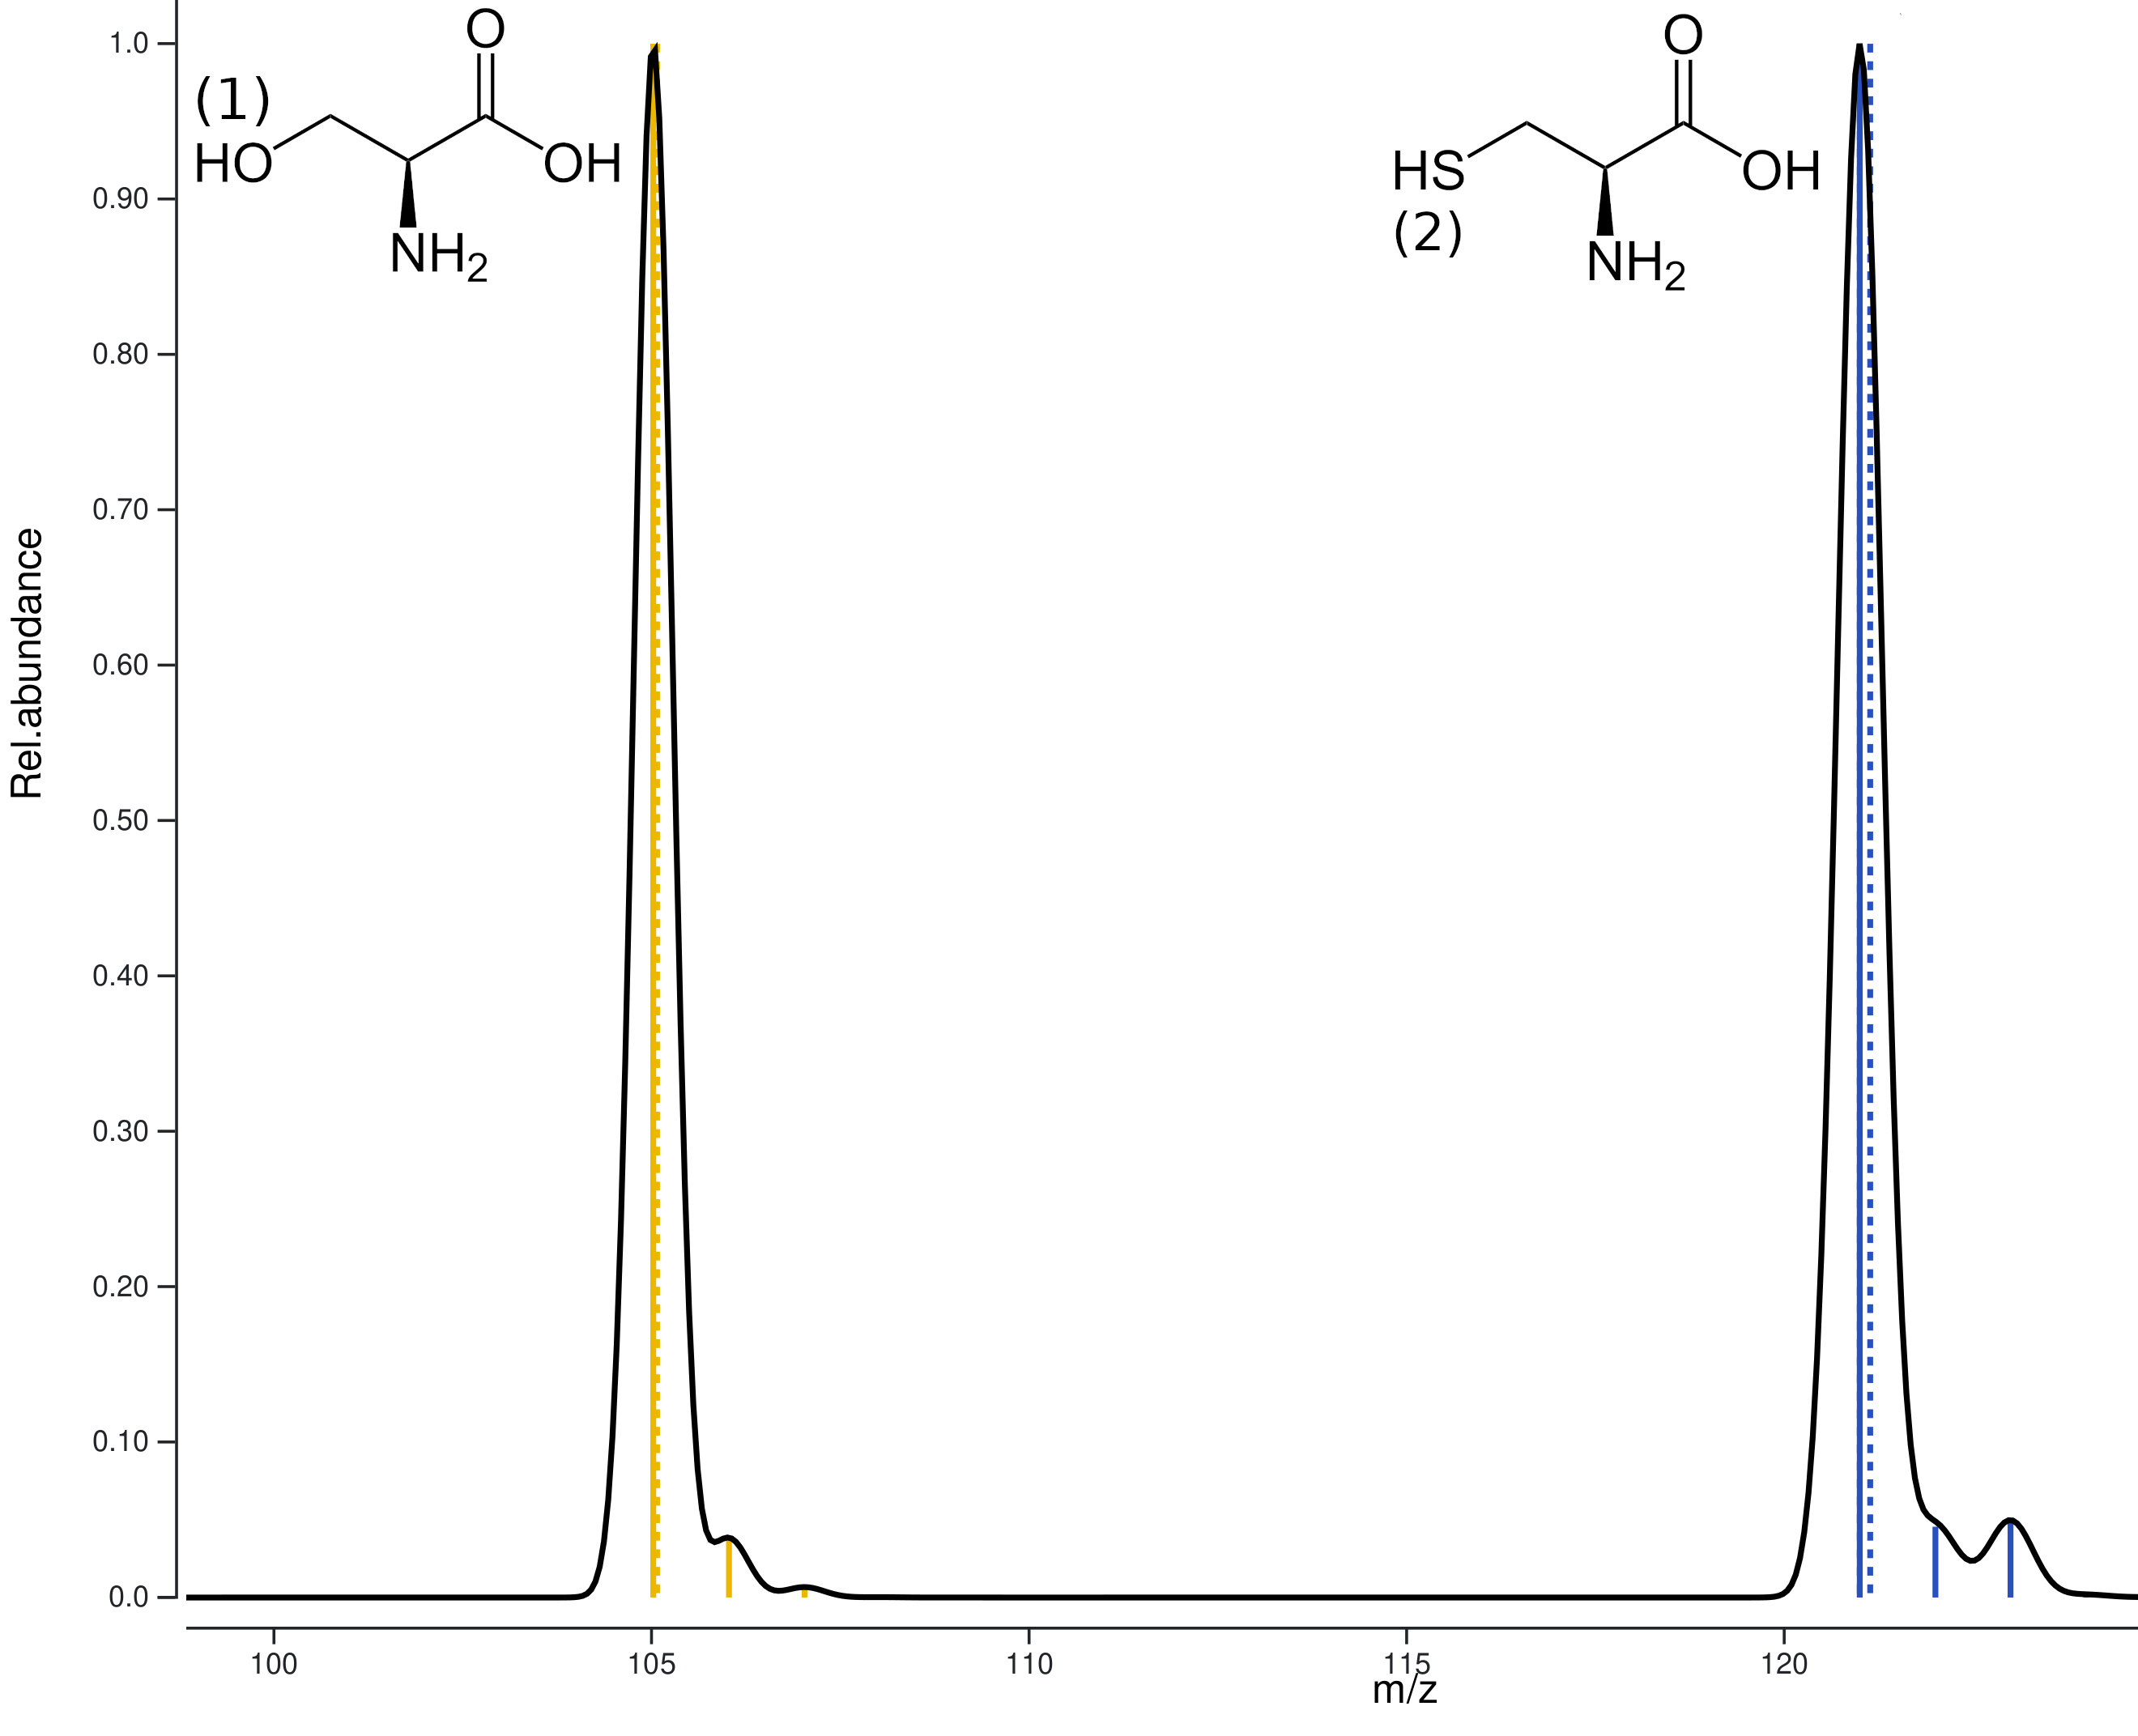
\includegraphics[width=0.75\textwidth]{./Resources/Simulated_Mass_Spectrum.png}
   \centering
   \caption{Computergeneriertes Massenspektrum von der Aminosäure \emph{Serin} (1) und \emph{Cystesin} (2). Peak von \emph{Serin} liegt bei 105; bei \emph{Systesin} um 121. y: relative Häufigkeit}
\end{figure}

Die Maxima werden \gerquot{Peaks} genannt und sind für eine Aminosäure an charakteristischer Position auf der $ x $-Achse. Obwohl sich die beiden Aminosäuren in der Abbildung \ref{fig:Sim_Mass_Spec} nur durch ein Atom unterscheiden (das linke Sauerstoffatom wurde durch ein Schwefelatom ersetzt) sind deren Massenspektren auf der $ x $-Achse weit voneinander entfernt und machen die beiden Aminosäuren dadurch sicher unterscheidbar.\\

Bei einzelnen Aminosäuren funktioniert die MS zuverlässig; bei Peptiden allerdings steht man vor dem Problem, dass das Massenspektrum unübersichtlicher wird und auch Peaks, die von Hintergrundrauschen stammen, schwerer herausgefiltert werden können. Abhilfe schafft hier die Tandem-Massenspektrometrie.

\subsection{Tandem-Massenspektrometrie (MS/MS)}\label{ss:Tandem_MS}
Bei der Tandem-Massenspektrometrie (MS/MS oder MS2) werden zwei MS Vorgänge hintereinander mit einer Probe durchgeführt. Die erste MS dient dazu Ionen aus einem bestimmten \massCharge Bereich auswählbar zu machen. Es entspricht also quasi einer Form der Filterung.

Vor der 2. MS werden die ausgewählten Reste einer Fragmentierung unterzogen. Bei einer Fragmentierung führt man Energie zu mit dem Ziel, dass die Ionen zerfallen und sog. Fragment-Ionen bilden. Diese Fragment-Ionen werden dann auf dem Massenspektrum nach der 2. MS sichtbar gemacht.

Fragment-Ionen sind kleiner als die ursprünglichen Ionen. So kann die 2. MS mit einer höheren Selektivität durchgeführt werden, welches Peaks durch Hintergrundrauschen verringert. Auch lassen sich Ionen besser identifizieren, die ein sehr ähnliches \massCharge-Verhältnis besitzen. Nach der 2. MS liegt eine Fülle an Fragment-Ionen-Peaks vor, aus denen sich die ursprünglichen Strukturinformationen ableiten lassen, da Ionen in spezifische Fragmente zerfallen \cite{Gross2013}. Zusammengefasst kann man sagen, dass das MS/MS Verfahren Ergebnisse höherer Güte erzeugt im Vergleich zur einfachen MS.

\section{De-Novo-Peptidsequenzierung mit \emph{pNovo+}}\label{s:pNovoPlusSeq}
Die \emph{pNovo+} Methode ist eine \gls{gls:DeNovo}, die mit einem \gls{gls:SpecGraph}en für die Auswertung der MS2-Spektren arbeitet und eine Erweiterung des \emph{pNovo} Verfahren darstellt \cite{pNovo}. Der Hauptansatz ist, dass zwei MS/MS Durchläufe mit jeweils verschiedenen Fragmentierungsmethoden\footnote{\emph{pNovo+} verwendet die higher energy
collisional dissociation (HCD) und die electron transfer dissociation (ETD) Fragmentierungsmethoden.} durchgeführt werden. Durch die Wahl einer anderen Fragmentierungsmethode ändert sich auch das MS2-Spektrum. Wenn nun Fragmentierungsmethoden verwendet werden, die möglichst komplementäre Spektren erzeugen, dann lässt sich durch das Zusammenführen der beiden MS2-Spektren die Qualität der Ergebnisse verbessern. Zum Beispiel lassen sich dadurch viele Peaks, die vom Hintergrundrauschen stammen, entfernen.

Für die Ermittlung der Sequenz eines Peptides wird zunächst ein Spektrums-Graph gebildet \dashAndSpace in Form eines DAG (directed acyclic graph). In diesem Graphen wird dann der längste Pfad bei gegebenen Start- und Endknoten berechnet. Die Reihenfolge der Knoten, die im längsten Pfad durchlaufen werden, stellt dann die Peptidsequenz dar.

\subsection{Vorverarbeitung der MS2-Spektren}\label{ss:Vorverarbeitung}
Bevor aus den MS2-Spektren der Spektrums-Graph gebildet werden kann, müssen die Daten vorverarbeitet werden. Für die Auswertung ist es von entscheidener Bedeutung, dass möglichst wenig Peaks verwendet werden, die vom Hintergrundrauschen stammen. Im weiteren Verlauf werden an einem exemplarischen MS2-Spektrum die Verarbeitungsschritte dargestellt.\\

Der erste Schritt ist das Verwenden des natürlichen Logarithmus der Intensitäten. Die Idee dabei ist, dass Hintergrundrauschen nicht überpriorisiert wird.

\begin{figure}[H]
   \centering
   \begin{minipage}[t]{.45\linewidth}
      \centering
      \begin{tikzpicture}[scale=\tikzScale, baseline=(current bounding box.center)]
         \draw [<->,thick] (0,\yAxisHeight) node (yaxis) [above] {\yAxisUnit}
         |- (\xAxisLength,0) node (xaxis) [right] {\xAxisUnit};
\draw[thick] (0.2, 0.0) -- (0.2, 2.3);
\draw[thick] (0.382, 0.0) -- (0.382, 1.7);
\draw[thick] (0.476, 0.0) -- (0.476, 2.7);
\draw[thick] (0.456, 0.0) -- (0.456, 1.8);
\draw[thick] (0.6859999999999999, 0.0) -- (0.6859999999999999, 2.7);
\draw[thick] (0.6839999999999999, 0.0) -- (0.6839999999999999, 1.8);
\draw[thick] (0.752, 0.0) -- (0.752, 1.1);
\draw[thick] (0.8200000000000001, 0.0) -- (0.8200000000000001, 2.2);
\draw[thick] (1.076, 0.0) -- (1.076, 1.5);
\draw[thick] (1.16, 0.0) -- (1.16, 1.9);
\draw[thick] (1.2120000000000002, 0.0) -- (1.2120000000000002, 2.0);
\draw[thick] (1.28, 0.0) -- (1.28, 1.9);
\draw[thick] (1.452, 0.0) -- (1.452, 1.3);
\draw[thick] (1.426, 0.0) -- (1.426, 1.9);
\draw[thick] (1.548, 0.0) -- (1.548, 1.9);
\draw[thick] (1.6740000000000002, 0.0) -- (1.6740000000000002, 1.5);
\draw[thick] (1.788, 0.0) -- (1.788, 2.5);
\draw[thick] (1.856, 0.0) -- (1.856, 2.3);
\draw[thick] (2.036, 0.0) -- (2.036, 1.7);
\draw[thick] (2.142, 0.0) -- (2.142, 1.6);
\draw[thick] (2.2520000000000002, 0.0) -- (2.2520000000000002, 2.0);
\draw[thick] (2.386, 0.0) -- (2.386, 1.6);
\draw[thick] (2.488, 0.0) -- (2.488, 2.9);
\draw[thick] (2.4739999999999998, 0.0) -- (2.4739999999999998, 2.7);
\draw[thick] (2.504, 0.0) -- (2.504, 2.0);
\draw[thick] (2.682, 0.0) -- (2.682, 2.0);
\draw[thick] (2.702, 0.0) -- (2.702, 2.5);
\draw[thick] (2.9259999999999997, 0.0) -- (2.9259999999999997, 2.8);
\draw[thick] (3.024, 0.0) -- (3.024, 2.4);
\draw[thick] (3.096, 0.0) -- (3.096, 1.8);
\draw[thick] (3.244, 0.0) -- (3.244, 2.6);
\draw[thick] (3.362, 0.0) -- (3.362, 1.9);
\draw[thick] (3.46, 0.0) -- (3.46, 2.3);
\draw[thick] (3.516, 0.0) -- (3.516, 1.1);
\draw[thick] (3.584, 0.0) -- (3.584, 1.8);
\draw[thick] (3.652, 0.0) -- (3.652, 2.0);
\draw[thick] (3.838, 0.0) -- (3.838, 1.5);
\draw[thick] (3.8819999999999997, 0.0) -- (3.8819999999999997, 2.6);
\draw[thick] (4.088, 0.0) -- (4.088, 2.6);
\draw[thick] (4.046, 0.0) -- (4.046, 1.1);
\draw[thick] (4.167999999999999, 0.0) -- (4.167999999999999, 2.0);
\draw[thick] (4.266, 0.0) -- (4.266, 2.4);
\draw[thick] (4.38, 0.0) -- (4.38, 1.1);
\draw[thick] (4.456, 0.0) -- (4.456, 2.2);
\draw[thick] (4.644, 0.0) -- (4.644, 2.6);
\draw[thick] (4.675999999999999, 0.0) -- (4.675999999999999, 2.5);
\draw[thick] (4.898000000000001, 0.0) -- (4.898000000000001, 1.2);
   \end{tikzpicture}%
   \end{minipage}%
   \textbf{$\rightarrow$} 
   \begin{minipage}[t]{.45\linewidth}
      \centering
      \begin{tikzpicture}[scale=\tikzScale, baseline=(current bounding box.center)]
      \draw [<->,thick] (0,\yAxisHeight) node (yaxis) [above] {\yAxisUnit}
      |- (\xAxisLength,0) node (xaxis) [right] {\xAxisUnit};
\draw[thick] (0.2, 0.0) -- (0.2, {ln(2.3)});
\draw[thick] (0.382, 0.0) -- (0.382, {ln(1.7)});
\draw[thick] (0.476, 0.0) -- (0.476, {ln(2.7)});
\draw[thick] (0.456, 0.0) -- (0.456, {ln(1.8)});
\draw[thick] (0.6859999999999999, 0.0) -- (0.6859999999999999, {ln(2.7)});
\draw[thick] (0.6839999999999999, 0.0) -- (0.6839999999999999, {ln(1.8)});
\draw[thick] (0.752, 0.0) -- (0.752, {ln(1.1)});
\draw[thick] (0.8200000000000001, 0.0) -- (0.8200000000000001, {ln(2.2)});
\draw[thick] (1.076, 0.0) -- (1.076, {ln(1.5)});
\draw[thick] (1.16, 0.0) -- (1.16, {ln(1.9)});
\draw[thick] (1.2120000000000002, 0.0) -- (1.2120000000000002, {ln(2.0)});
\draw[thick] (1.28, 0.0) -- (1.28, {ln(1.9)});
\draw[thick] (1.452, 0.0) -- (1.452, {ln(1.3)});
\draw[thick] (1.426, 0.0) -- (1.426, {ln(1.9)});
\draw[thick] (1.548, 0.0) -- (1.548, {ln(1.9)});
\draw[thick] (1.6740000000000002, 0.0) -- (1.6740000000000002, {ln(1.5)});
\draw[thick] (1.788, 0.0) -- (1.788, {ln(2.5)});
\draw[thick] (1.856, 0.0) -- (1.856, {ln(2.3)});
\draw[thick] (2.036, 0.0) -- (2.036, {ln(1.7)});
\draw[thick] (2.142, 0.0) -- (2.142, {ln(1.6)});
\draw[thick] (2.2520000000000002, 0.0) -- (2.2520000000000002, {ln(2.0)});
\draw[thick] (2.386, 0.0) -- (2.386, {ln(1.6)});
\draw[thick] (2.488, 0.0) -- (2.488, {ln(2.9)});
\draw[thick] (2.4739999999999998, 0.0) -- (2.4739999999999998, {ln(2.7)});
\draw[thick] (2.504, 0.0) -- (2.504, {ln(2.0)});
\draw[thick] (2.682, 0.0) -- (2.682, {ln(2.0)});
\draw[thick] (2.702, 0.0) -- (2.702, {ln(2.5)});
\draw[thick] (2.9259999999999997, 0.0) -- (2.9259999999999997, {ln(2.8)});
\draw[thick] (3.024, 0.0) -- (3.024, {ln(2.4)});
\draw[thick] (3.096, 0.0) -- (3.096, {ln(1.8)});
\draw[thick] (3.244, 0.0) -- (3.244, {ln(2.6)});
\draw[thick] (3.362, 0.0) -- (3.362, {ln(1.9)});
\draw[thick] (3.46, 0.0) -- (3.46, {ln(2.3)});
\draw[thick] (3.516, 0.0) -- (3.516, {ln(1.1)});
\draw[thick] (3.584, 0.0) -- (3.584, {ln(1.8)});
\draw[thick] (3.652, 0.0) -- (3.652, {ln(2.0)});
\draw[thick] (3.838, 0.0) -- (3.838, {ln(1.5)});
\draw[thick] (3.8819999999999997, 0.0) -- (3.8819999999999997, {ln(2.6)});
\draw[thick] (4.088, 0.0) -- (4.088, {ln(2.6)});
\draw[thick] (4.046, 0.0) -- (4.046, {ln(1.1)});
\draw[thick] (4.167999999999999, 0.0) -- (4.167999999999999, {ln(2.0)});
\draw[thick] (4.266, 0.0) -- (4.266, {ln(2.4)});
\draw[thick] (4.38, 0.0) -- (4.38, {ln(1.1)});
\draw[thick] (4.456, 0.0) -- (4.456, {ln(2.2)});
\draw[thick] (4.644, 0.0) -- (4.644, {ln(2.6)});
\draw[thick] (4.675999999999999, 0.0) -- (4.675999999999999, {ln(2.5)});
\draw[thick] (4.898000000000001, 0.0) -- (4.898000000000001, {ln(1.2)});
      \end{tikzpicture}
      \end{minipage}
      \caption{Anwendung des $ ln $ auf einem exemplarischen MS2-Spektrum.}
\end{figure}

Für das Verständnis des nächsten Schrittes muss man sich in Erinnerung rufen, dass eine gleiche Aminosäure keineswegs immer die gleiche Masse hat. Durch Isotope existiert eine gewisse \gerquot{Massenbandbreite} für ein und dieselbe Aminosäure. MS Systeme sind heute so genau, dass sie diese Differenzen erkennen. Dies hat den ungewollten Effekt, dass mehrere Peaks zu einer Aminosäure gehören können \cite{IsotopicDistributionMS}. Gleichzeitig können die \gerquot{Massenbandbreiten} zweier Aminosäuren sich überschneiden, sodass im ungünstigen Fall zwei Peaks kaum unterscheidbar nebeneinander liegen.\\

Eine Möglichkeit mit dieser Problematik umzugehen ist die Verwendung der monoisotopischen Masse. Die monoisotopische Masse ist die \gerquot{[...] exact mass of the most abundant naturally occurring stable isotope determined relative to the mass of 12 C, which is assigned the exact value of 12.0000.} \cite{MonoisotopicMass}. Ohne dabei jetzt tiefer ins Detail zu gehen kann man sagen, dass alle Peaks, deren Intensität mit einer möglichen monoisotopischen Masse übereinstimmen, auf jeden Fall einer Aminosäure entsprechen und (höchstwahrscheinlich)\footnote{Natürlich ist es möglich, dass das Rauschen zufällig einer monoisotopischen Masse entspricht. Die Wahrscheinlichkeit dafür ist allerdings sehr gering.} kein Hintergrundrauschen sind \cite{MassDefectMS}. Diese Peaks bekommen eine sogennante \emph{charge state}.\\

Der Algorithmus verwendet die \emph{charge state} Peaks als Ausganspunkte für weitere Berechnungen. Wenn die \massCharge Differenz zu einem anderen Peak einem Peptidfragment entspricht, dann stammt dieser Peak höchstwahrscheinlich von einem Fragment. Insgesamt werden damit die relevanten Peptidfragmente herausgeholt. Abbildung \ref{MonoisotopicMassFiltering} zeigt das Ergebnis nach den beiden zuvor genannten Schritten.

\begin{figure}[H]\label{MonoisotopicMassFiltering}
   \centering
   \begin{minipage}[t]{.45\linewidth}
      \centering
      \begin{tikzpicture}[scale=\tikzScale, baseline=(current bounding box.center)]
         \draw [<->,thick] (0,\yAxisHeight) node (yaxis) [above] {\yAxisUnit}
         |- (\xAxisLength,0) node (xaxis) [right] {\xAxisUnit};
\draw[thick] (0.2, 0.0) -- (0.2, {ln(2.3)});
\draw[color=blue!85!,opacity=.55,thick] (0.382, 0.0) -- (0.382, {ln(1.7)});
\draw[color=blue!85!,opacity=.55,thick] (0.476, 0.0) -- (0.476, {ln(2.7)});
\draw[color=magenta,thick] (0.456, 0.0) -- (0.456, {ln(1.8)});
\draw[color=blue!85!,opacity=.55,thick] (0.6859999999999999, 0.0) -- (0.6859999999999999, {ln(2.7)});
\draw[color=blue!85!,opacity=.55,thick] (0.6839999999999999, 0.0) -- (0.6839999999999999, {ln(1.8)});
\draw[thick] (0.752, 0.0) -- (0.752, {ln(1.1)});
\draw[thick] (0.8200000000000001, 0.0) -- (0.8200000000000001, {ln(2.2)});
\draw[thick] (1.076, 0.0) -- (1.076, {ln(1.5)});
\draw[thick] (1.16, 0.0) -- (1.16, {ln(1.9)});
\draw[thick] (1.2120000000000002, 0.0) -- (1.2120000000000002, {ln(2.0)});
\draw[thick] (1.28, 0.0) -- (1.28, {ln(1.9)});
\draw[color=blue!85!,opacity=.55,thick] (1.452, 0.0) -- (1.452, {ln(1.3)});
\draw[color=blue!85!,opacity=.55,thick] (1.426, 0.0) -- (1.426, {ln(1.9)});
\draw[color=magenta,thick] (1.548, 0.0) -- (1.548, {ln(1.9)});
\draw[color=blue!85!,opacity=.55,thick] (1.6740000000000002, 0.0) -- (1.6740000000000002, {ln(1.5)});
\draw[color=blue!85!,opacity=.55,thick] (1.788, 0.0) -- (1.788, {ln(2.5)});
\draw[thick] (1.856, 0.0) -- (1.856, {ln(2.3)});
\draw[thick] (2.036, 0.0) -- (2.036, {ln(1.7)});
\draw[thick] (2.142, 0.0) -- (2.142, {ln(1.6)});
\draw[thick] (2.2520000000000002, 0.0) -- (2.2520000000000002, {ln(2.0)});
\draw[thick] (2.386, 0.0) -- (2.386, {ln(1.6)});
\draw[color=blue!85!,opacity=.55,thick] (2.488, 0.0) -- (2.488, {ln(2.9)});
\draw[thick] (2.4739999999999998, 0.0) -- (2.4739999999999998, {ln(2.7)});
\draw[color=blue!85!,opacity=.55,thick] (2.504, 0.0) -- (2.504, {ln(2.0)});
\draw[color=magenta,thick] (2.682, 0.0) -- (2.682, {ln(2.0)});
\draw[color=blue!85!,opacity=.55,thick] (2.702, 0.0) -- (2.702, {ln(2.5)});
\draw[thick] (2.9259999999999997, 0.0) -- (2.9259999999999997, {ln(2.8)});
\draw[thick] (3.024, 0.0) -- (3.024, {ln(2.4)});
\draw[thick] (3.096, 0.0) -- (3.096, {ln(1.8)});
\draw[thick] (3.244, 0.0) -- (3.244, {ln(2.6)});
\draw[thick] (3.362, 0.0) -- (3.362, {ln(1.9)});
\draw[color=blue!85!,opacity=.55,thick] (3.46, 0.0) -- (3.46, {ln(2.3)});
\draw[color=blue!85!,opacity=.55,thick] (3.516, 0.0) -- (3.516, {ln(1.1)});
\draw[color=blue!85!,opacity=.55,thick] (3.584, 0.0) -- (3.584, {ln(1.8)});
\draw[color=magenta,thick] (3.652, 0.0) -- (3.652, {ln(2.0)});
\draw[color=blue!85!,opacity=.55,thick] (3.838, 0.0) -- (3.838, {ln(1.5)});
\draw[color=blue!85!,opacity=.55,thick] (3.8819999999999997, 0.0) -- (3.8819999999999997, {ln(2.6)});
\draw[thick] (4.088, 0.0) -- (4.088, {ln(2.6)});
\draw[thick] (4.046, 0.0) -- (4.046, {ln(1.1)});
\draw[thick] (4.167999999999999, 0.0) -- (4.167999999999999, {ln(2.0)});
\draw[thick] (4.266, 0.0) -- (4.266, {ln(2.4)});
\draw[color=blue!85!,opacity=.55,thick] (4.38, 0.0) -- (4.38, {ln(1.1)});
\draw[color=blue!85!,opacity=.55,thick] (4.456, 0.0) -- (4.456, {ln(2.2)});
\draw[color=magenta,thick] (4.644, 0.0) -- (4.644, {ln(2.6)});
\draw[color=blue!85!,opacity=.55,thick] (4.675999999999999, 0.0) -- (4.675999999999999, {ln(2.5)});
\draw[color=blue!85!,opacity=.55,thick] (4.898000000000001, 0.0) -- (4.898000000000001, {ln(1.2)});
   \end{tikzpicture}%
   \end{minipage}%
   \textbf{$\rightarrow$} 
   \begin{minipage}[t]{.45\linewidth}
      \centering
      \begin{tikzpicture}[scale=\tikzScale, baseline=(current bounding box.center)]
      \draw [<->,thick] (0,\yAxisHeight) node (yaxis) [above] {\yAxisUnit}
      |- (\xAxisLength,0) node (xaxis) [right] {\xAxisUnit};
\draw[color=blue!85!,opacity=.55,thick] (0.382, 0.0) -- (0.382, {ln(1.7)});
\draw[color=blue!85!,opacity=.55,thick] (0.476, 0.0) -- (0.476, {ln(2.7)});
\draw[color=magenta,thick] (0.456, 0.0) -- (0.456, {ln(1.8)});
\draw[color=blue!85!,opacity=.55,thick] (0.6859999999999999, 0.0) -- (0.6859999999999999, {ln(2.7)});
\draw[color=blue!85!,opacity=.55,thick] (0.6839999999999999, 0.0) -- (0.6839999999999999, {ln(1.8)});
\draw[color=blue!85!,opacity=.55,thick] (1.452, 0.0) -- (1.452, {ln(1.3)});
\draw[color=blue!85!,opacity=.55,thick] (1.426, 0.0) -- (1.426, {ln(1.9)});
\draw[color=magenta,thick] (1.548, 0.0) -- (1.548, {ln(1.9)});
\draw[color=blue!85!,opacity=.55,thick] (1.6740000000000002, 0.0) -- (1.6740000000000002, {ln(1.5)});
\draw[color=blue!85!,opacity=.55,thick] (1.788, 0.0) -- (1.788, {ln(2.5)});
\draw[color=blue!85!,opacity=.55,thick] (2.488, 0.0) -- (2.488, {ln(2.9)});
\draw[color=blue!85!,opacity=.55,thick] (2.504, 0.0) -- (2.504, {ln(2.0)});
\draw[color=magenta,thick] (2.682, 0.0) -- (2.682, {ln(2.0)});
\draw[color=blue!85!,opacity=.55,thick] (2.702, 0.0) -- (2.702, {ln(2.5)});
\draw[color=blue!85!,opacity=.55,thick] (3.46, 0.0) -- (3.46, {ln(2.3)});
\draw[color=blue!85!,opacity=.55,thick] (3.516, 0.0) -- (3.516, {ln(1.1)});
\draw[color=blue!85!,opacity=.55,thick] (3.584, 0.0) -- (3.584, {ln(1.8)});
\draw[color=magenta,thick] (3.652, 0.0) -- (3.652, {ln(2.0)});
\draw[color=blue!85!,opacity=.55,thick] (3.838, 0.0) -- (3.838, {ln(1.5)});
\draw[color=blue!85!,opacity=.55,thick] (3.8819999999999997, 0.0) -- (3.8819999999999997, {ln(2.6)});
\draw[color=blue!85!,opacity=.55,thick] (4.38, 0.0) -- (4.38, {ln(1.1)});
\draw[color=blue!85!,opacity=.55,thick] (4.456, 0.0) -- (4.456, {ln(2.2)});
\draw[color=magenta,thick] (4.644, 0.0) -- (4.644, {ln(2.6)});
\draw[color=blue!85!,opacity=.55,thick] (4.675999999999999, 0.0) -- (4.675999999999999, {ln(2.5)});
\draw[color=blue!85!,opacity=.55,thick] (4.898000000000001, 0.0) -- (4.898000000000001, {ln(1.2)});
      \end{tikzpicture}
      \end{minipage}
      \caption{Entfernen von Peaks, die keiner monoisotopischen Masse entsprechen oder benachbart mit einer Differenz von einem Fragment-Ion sind.}
\end{figure}

Tatsächlich ist die Verarbeitung an dieser Stelle noch etwas komplexer. So existieren auch noch sogenannte \emph{isotopic cluster}\footnote{Definition eines \emph{isotopic cluster} nach IUPAC: \gerquot{Group of peaks representing ions of the same elemental composition, but different isotopic compositions.} \cite[1556]{IUPACDefinitions}}, die gesondert verarbeitet werden. Für das grundsätzliche Prinzip ist dieses Detail allerdings weniger relevant.\\

Im letzten Vorberarbeitungsschritt werden Peaks aus einem irrelevanten \massCharge Bereich entfernt und naheliegende Peaks werden zusammengefasst, indem der Mittelwert sowol des \massCharge Wertes als auch der der Intensität besimmt wird. Üblicherweise liegt der Bereich für das Zusammenfassen bei $ +- 20 ppm $.

\begin{figure}[H]
   \centering
   \begin{minipage}[t]{.45\linewidth}
      \centering
      \begin{tikzpicture}[scale=\tikzScale, baseline=(current bounding box.center)]
         \draw [<->,thick] (0,\yAxisHeight) node (yaxis) [above] {\yAxisUnit}
         |- (\xAxisLength,0) node (xaxis) [right] {\xAxisUnit};
\draw[thick] (0.382, 0.0) -- (0.382, {ln(1.7)});
\draw[thick] (0.476, 0.0) -- (0.476, {ln(2.7)});
\draw[thick] (0.456, 0.0) -- (0.456, {ln(1.8)});
\draw[thick] (0.6859999999999999, 0.0) -- (0.6859999999999999, {ln(2.7)});
\draw[thick] (0.6839999999999999, 0.0) -- (0.6839999999999999, {ln(1.8)});
\draw[color=red,thick] (1.452, 0.0) -- (1.452, {ln(1.3)});
\draw[color=red,thick] (1.426, 0.0) -- (1.426, {ln(1.9)});
\draw[thick] (1.548, 0.0) -- (1.548, {ln(1.9)});
\draw[thick] (1.6740000000000002, 0.0) -- (1.6740000000000002, {ln(1.5)});
\draw[thick] (1.788, 0.0) -- (1.788, {ln(2.5)});
\draw[color=red,thick] (2.488, 0.0) -- (2.488, {ln(2.9)});
\draw[color=red,thick] (2.504, 0.0) -- (2.504, {ln(2.0)});
\draw[color=red,thick] (2.682, 0.0) -- (2.682, {ln(2.0)});
\draw[color=red,thick] (2.702, 0.0) -- (2.702, {ln(2.5)});
\draw[thick] (3.46, 0.0) -- (3.46, {ln(2.3)});
\draw[thick] (3.516, 0.0) -- (3.516, {ln(1.1)});
\draw[thick] (3.584, 0.0) -- (3.584, {ln(1.8)});
\draw[thick] (3.652, 0.0) -- (3.652, {ln(2.0)});
\draw[color=red,thick] (3.838, 0.0) -- (3.838, {ln(1.5)});
\draw[color=red,thick] (3.8819999999999997, 0.0) -- (3.8819999999999997, {ln(2.6)});
\draw[thick] (4.38, 0.0) -- (4.38, {ln(1.1)});
\draw[thick] (4.456, 0.0) -- (4.456, {ln(2.2)});
\draw[thick] (4.644, 0.0) -- (4.644, {ln(2.6)});
\draw[thick] (4.675999999999999, 0.0) -- (4.675999999999999, {ln(2.5)});
\draw[thick] (4.898000000000001, 0.0) -- (4.898000000000001, {ln(1.2)});

\fill[red!25!,opacity=.25] (0,0) rectangle (1,\yAxisHeight-\axisColorOffset);
         \fill[red!25!,opacity=.25] (\xAxisLength-1,0) rectangle (\xAxisLength-\axisColorOffset,\yAxisHeight-\axisColorOffset);
         \fill[green!25!,opacity=.25] (1,0) rectangle (\xAxisLength-1,\yAxisHeight-\axisColorOffset);
   \end{tikzpicture}%
   \end{minipage}%
   \textbf{$\rightarrow$} 
   \begin{minipage}[t]{.45\linewidth}
      \centering
      \begin{tikzpicture}[scale=\tikzScale, baseline=(current bounding box.center)]
      \draw [<->,thick] (0,\yAxisHeight) node (yaxis) [above] {\yAxisUnit}
      |- (\xAxisLength,0) node (xaxis) [right] {\xAxisUnit};
%\draw[color=red,thick] (1.452, 0.0) -- (1.452, {ln(1.3)});
%\draw[color=red,thick] (1.426, 0.0) -- (1.426, {ln(1.9)});
\draw[color=red,ultra thick] ({(1.452+1.426)/2}, 0.0) -- ({(1.452+1.426)/2}, {(ln(1.3)+ln(1.9))/2});

\draw[thick] (1.548, 0.0) -- (1.548, {ln(1.9)});
\draw[thick] (1.6740000000000002, 0.0) -- (1.6740000000000002, {ln(1.5)});
\draw[thick] (1.788, 0.0) -- (1.788, {ln(2.5)});

%\draw[color=red,thick] (2.488, 0.0) -- (2.488, {ln(2.9)});
%\draw[color=red,thick] (2.504, 0.0) -- (2.504, {ln(2.0)});
\draw[color=red,ultra thick] ({(2.488+2.504)/2}, 0.0) -- ({(2.488+2.504)/2}, {(ln(2.9)+ln(2.0))/2});

%\draw[color=red,thick] (2.682, 0.0) -- (2.682, {ln(2.0)});
%\draw[color=red,thick] (2.702, 0.0) -- (2.702, {ln(2.5)});
\draw[color=red,ultra thick] ({(2.682+2.702)/2}, 0.0) -- ({(2.682+2.702)/2}, {(ln(2.0+ln(2.5))/2});

\draw[thick] (3.46, 0.0) -- (3.46, {ln(2.3)});
\draw[thick] (3.516, 0.0) -- (3.516, {ln(1.1)});
\draw[thick] (3.584, 0.0) -- (3.584, {ln(1.8)});
\draw[thick] (3.652, 0.0) -- (3.652, {ln(2.0)});

%\draw[color=red,thick] (3.838, 0.0) -- (3.838, {ln(1.5)});
%\draw[color=red,thick] (3.8819999999999997, 0.0) -- (3.8819999999999997,{ln(2.6)});
\draw[color=red,ultra thick] ({(3.838+3.8819999999999997)/2}, 0.0) -- ({(3.838+3.8819999999999997)/2}, {(ln(1.5)+ln(2.6))/2});

\fill[red!25!,opacity=.25] (0,0) rectangle (1,\yAxisHeight-\axisColorOffset);
         \fill[red!25!,opacity=.25] (\xAxisLength-1,0) rectangle (\xAxisLength-\axisColorOffset,\yAxisHeight-\axisColorOffset);
         \fill[green!25!,opacity=.25] (1,0) rectangle (\xAxisLength-1,\yAxisHeight-\axisColorOffset);
      \end{tikzpicture}
      \end{minipage}
      \caption{Entfernen von Peaks aus einem irrelevanten \massCharge Bereich und zusammenfassen naheliegender Peaks. Rot markierte Peaks sind jene, die zusammengefasst werden.}
\end{figure}

\subsection{Bildung eines Spektrums-Graphen}\label{ss:BildungSpekGraph}
Der Spektrums-Graph wird aus einem vorverarbeiteten MS2-Spektrum (siehe Kapitel: \ref{ss:Vorverarbeitung}) gebildet. Im initialen Zustand werden die Peaks als Knoten interpretiert. Dazu kommt ein Start- und Endknoten. Jedem Knoten wird eine Masse zugeordet; im initialen Zustand bekommt der Startknoten die Masse 0 und der Endknoten die Masse des vorherigen Knotens minus der Masse des Wassers ($ 18,02 $). Die Masse der übrigen Knoten entsprechen ihren jeweils korrespondierenden \massCharge Wert. Die gerichteten Kanten werden zwischen einem Knotenpaar hinzugefügt, wenn die Differenz deren Masse gleich ist mit der Masse von ein oder zwei Aminosäuren.

\subsection{Identifikation der Aminosäuresequenz}
Der gebildete DAG kann mit klassischen Algorithmen, die den längsten Pfad suchen, durchlaufen werden. Bezogen auf die Graphentheorie entspricht die Ermittlung der Aminosäurensequenz dem Suchen eines bestimmten Pfades \dashAndSpace und nicht nach irgendeinem Pfad. Daher muss der Algorithmus mittels einer Breitensuche arbeiten, um alle möglichen Pfade zu bestimmen.

In aller Regel wird es mehrere Pfade geben. Bestimmte Sequenzen sind wahrscheinlicher als andere. So sind Pfade mit Kanten, die wegen der Massendifferenz von genau einer Aminosäure gebildet wurden, wahrscheinlicher \cite{pNovoPlus}. Alle Pfade bekommen mittels einer Scoring-Funktion einen Wert zugewiesen. Der Pfad mit dem höchsten Scoring-Wert ist wahrscheinlich das richtige Ergebnis. Die Scoring-Funktion berücksichtigt unter anderem wie viele Fragmente, die einer bestimmten Aminosäure zugeordet werden können, im MS2-Spektrum vorhanden sind \cite{pNovo}. Die Sequenz mit dem höchsten Scoring-Wert ist das Endergebnis.

\section{De-Novo-Peptidsequenzierung mit \emph{Open-pNovo}}\label{s:OpenpNovoSeq}
Bei Proteinen können posttranslationale Proteinmodifikationen (PTM) auftreten. PTMs sind Ereignisse, bei denen sich Änderungen im Protein einstellen \cite{Mann2003}; teilweise sind die Änderungen von einer Zelle erwünscht \dashAndSpace teilweise stammen sie aber auch zum Beispiel von unerwünschten Wechselwirkungen nebeneinanderliegenden Aminosäuren. Ein Teil dieser PTMs führen zu einer Änderung der Aminosäuresequenz. Dies ist für die \gls{gls:DeNovo} nicht weiter problematisch, da sowieso ohne eine Datenbank gearbeitet wird, sodass solche PTMs nicht einmal auffallen würden. Andere PTMs hingegen haben die Auswirkung, dass Stoffe gebildet werden, die nicht mehr zu der Gruppe der proteinogenen Aminosäuren gehören. Proteinogene Aminosäuren sind jene Aminosäuren, die für den Bau von Proteinen verwendet werden. Der Effekt ist also, dass Stoffe (oder deren Fragmente) bei einem Massenspektrum angezeigt werden, die kein Teil eines Peptids sein können. Bei der Sequenzierung von Peptidfragmenten muss dies daher berücksichtigt werden.
Wenn im weiteren Verlauf von PTMs gesprochen wird, dann sind solche gemeint, die für die \gls{gls:DeNovo} relevant sind.

Open-pNovo ist ein \gls{gls:DeNovo}sverfahren, welches auf pNovo+ Tool aufbaut und versucht die Problematik mit den PTMs zu lösen.

\subsection{PTMs im konstruierten DAG}
Die Konvertierung eines MS2-Spektrums läuft bis zum DAG analog ab wie in den Kapiteln \ref{ss:Vorverarbeitung} und \ref{ss:BildungSpekGraph} für pNovo+. Der Unterschied ist nun, dass es zwei Arten von Kanten gibt:

\begin{itemize}
   \item \gerquot{Normale} Kanten: Kanten, die gebildet werden, wie es bereits für \emph{pNovo+} gezeigt wurde. 
   \item \gerquot{Modifizierte} Kanten: Kanten, die zum Grahpen hinzugefügt werden, wenn die Massendifferenz zweier Knoten der Masse einer Aminosäure plus der Masse einer möglichen PTM-Änderung entspricht. 
\end{itemize}

Eine Liste aller PTMs in der Datenbank Unimod (sowohl relevante als auch nicht relevante) beinhaltet aktuell 1510 Einträge\footnote{Siehe: \url{https://www.ebi.ac.uk/ols/ontologies/unimod}} (Stand: 18.04.2022). Für die modifizierten Kanten gibt es insgesamt $ 1510 * 20 = 30200 $ mögliche Differenzen, wobei viele davon nicht relevante PTMs sind. Zum Vergleich: bei den normalen Kanten gibt es $ 20^2 = 400 $ mögliche Differenzen.

Die hohe Anzahl an Differenzen für modifizierte Kanten hat die Konsequenz, dass viele Knoten zufällig verbunden werden und dass dadurch die Genauigkeit der Ergebnisse abnimmt. Dieses Problem kann man durch eine geringere Liste an möglichen PTMs abfedern, allerdings mit einem Verlust  der Genauigkeit auf Seiten der PTMs. Es ist hier also eine Abwägung.

\subsection{Evaluierung von Open-pNovo}
Open-pNovo wurde sowohl auf drei realen als auch auf drei generierten Testdaten getestet. Tabelle \ref{tab:OpenPNovoResults} zeigt die Ergebnisse im Vergleich zu pNovo+ und zwei anderen Algorithmen. Die Datensätze enthielten die am häufigsten vorkommenden PTMs.

\begin{table}[H]
    \centering
    \begin{tabular}{l|c|c|c|c}
        \toprule
        \textbf{Testdatensätze} & \textbf{Open-pNovo+} & \textbf{pNovo+} & \textbf{PEAKS} & \textbf{Novor} \\
        \midrule
        Real (20259) & $76,3 \%$ & $68,5 \%$ & $65,8 \%$ & $39,9 \%$ \\
        Generiert (17877) & $77,8 \%$ & $0,6 \%$ & $0,5 \%$ & $0,2 \%$ \\
        \bottomrule
    \end{tabular}
    \newline
    \caption{Vergleich der durchschnittlichen richtigen \gls{gls:DeNovo} Peptidsequenzierungen von Open-pNovo und anderen Algorithmen \cite[650]{OpenPNovo}.}
    \label{tab:OpenPNovoResults}
\end{table}

Die enorm schlechten Ergebnisse der anderen Algorithmen bei den generierten Testdaten ist ein Nebeneffekt des Ziels bei der Testdatengenerierung. Denn diese wurden so ausgelegt, um die Grenzen von Open-pNovo+ zu ermitteln \cite[649]{OpenPNovo}. Eine Aussagekraft haben diese Ergebnisse also nicht. Allerdings auch bei realen Testdaten zeigt sich Open-pNovo als voll konkurrenzfähig gegenüber den anderen Algorithmen.

Noch besser zeigt sich Open-pNovo, wenn der Recall Wert betrachtet wird \dashAndSpace also die Anzahl an verschiedenen PSMs, die erkannt wurden. In diesem Fall ist der Abstand zu den anderen Algorithmen deutlich größer geworden.

\begin{table}[H]
    \centering
    \begin{tabular}{l|c|c|c|c}
        \toprule
        \textbf{Testdatensätze} & \textbf{Open-pNovo+} & \textbf{pNovo+} & \textbf{PEAKS} & \textbf{Novor} \\
        \midrule
        Real (5034) & $61,6 \%$ & $31,3 \%$ & $32,0 \%$ & $13,7 \%$ \\
        \bottomrule
    \end{tabular}
    \newline
    \caption{Vergleich der durchschnittlichen Recall Werte einer \gls{gls:DeNovo} Peptidsequenzierungen von Open-pNovo und anderen Algorithmen \cite[650]{OpenPNovo}.}
    \label{tab:OpenPNovoResultsRecall}
\end{table}

\subsection{Zusammenfassung}


% Die \gls{gls:DeNovo} nutzt die sogenannte \gls{gls:TMassSpek} für die Bestimmung der Peptidsequenz. Dabei wird die physikalische Eigenschaft ausgenutzt, dass jedes Atom bzw. jedes Molekül \dashAndSpace wenn es einer \gls{gls:Ionisation} unterzogen wurde \dashAndSpace ein charakteristisches \gls{gls:MassSpek} besitzt. Das \gls{gls:MassSpek} stellt also eine Art \gerquot{Fingerabdruck} eines Moleküls dar und macht dieses ermittelbar.

% U.U. eine Beispielgrafik eines Massenspektrums hinzufuegen ...

\subsubsection{\glsentrytext{gls:TMassSpek} bei größeren Molekülen}
Bei größeren Molekülen (wie einem Protein) führt die \gls{gls:Ionisation} dazu, dass das Molekül in kleinere spezifische Ionen zerfällt (sog. Fragmentierung). Die Fragmentierungsinformationen einer \gls{gls:DeNovo} sind meist unvollständig, da fehlende Daten bei einem Fragmentierungsschritt die Güte des Endergebnisses negativ beeinflusst. Dies wird insbesondere dann ein Problem, wenn unbekannte Änderungen in einer Peptidsequenz vorhanden sind.

Um dieses Problem zu verringern können unterschiedliche Techniken parallel eingesetzt werden, welche verschiedene Fragmente erzeugen und daher auch verschiedenartige \glspl{gls:MassSpek} zur Folge haben.\footnote{Konkret: Es wird sowohl das \gls{acr:HCD} als auch das \gls{acr:ETD} Verfahren angewendet.}

\subsection{Datenaufbereitung}
Typischerweise betrachtet man die sog. \gerquot{\glspl{gls:Peak}} in den \glspl{gls:MassSpek}. Jeder \gls{gls:Peak} stellt ein unterschiedliches Ion dar. Dazu kommen Messungenauigkeiten sowie Hintergrundrauschen. Durch die hohe Anzahl an möglichen Ionen kann nicht ohne weiteres differenziert werden, welcher der \glspl{gls:Peak} von welchen Ionen erzeugt wurden und welche nicht.

% Frage an Dominik: Ist hier eine einfache Auflistung an Techniken für die Datenaufbereitung besser?
Der Algorithmus für die Datenaufbereitung berechnet den natürlichen Logarithmus von den Intensitäten der \glspl{gls:Peak}, um Hintergrundrauschen und Messungenauigkeiten nicht überzupriorisieren. Zusätzlich dazu werden \glspl{gls:Peak}, die in einem Toleranzbereich nebeneinander liegen, zusammengefasst. Am Ende werden die \glspl{gls:Peak} entfernt, bei denen bekannt ist, dass es sich nicht um relevante Ionen handeln kann. (z.B. \glspl{gls:Peak} von Isotopen)

\begin{figure}[H]
   \centering
   \begin{minipage}[t]{.4\linewidth}
      \centering
      \begin{tikzpicture}[scale=\tikzScale, baseline=(current bounding box.center)]
         \draw [<->,thick] (0,2.75) node (yaxis) [above] {\yAxisUnit}
         |- (3,0) node (xaxis) [right] {\xAxisUnit};

         \draw[thick] (0.2,0) -- (0.2,1.1);
         \draw[thick] (0.3,0) -- (0.3,1.6);
         \draw[thick] (0.6,0) -- (0.6,1.7);
         \draw[thick] (0.8,0) -- (0.8,1.2);
         \draw[thick] (1.0,0) -- (1.0,1.1);

         \draw[color=red,thick] (1.2,0) -- (1.2,2.65);
         \draw[thick] (1.4,0) -- (1.4,1.4);
         \draw[thick] (1.6,0) -- (1.6,1.2);
         \draw[thick] (1.8,0) -- (1.8,1.3);
         \draw[thick] (2.0,0) -- (2.0,1.8);

         \draw[thick] (1.1,0) -- (1.1,2.0);
         \draw[color=red,thick] (0.35,0) -- (0.35,2.25);
         \draw[thick] (1.9,0) -- (1.9,1.4);
         \draw[color=red,thick] (2.2,0) -- (2.2,2.6);
         \draw[thick] (2.5,0) -- (2.5,1.25);

         \draw[thick] (2.7,0) -- (2.7,1.1);
         \foreach \x in {1,...,6}
         {
            \draw[thick] (1.2+\x*0.05,0) -- (1.2+\x*0.05,1.0+\x*0.15);
         }
      \end{tikzpicture}%
      % \subcaption{Exemplarische Rohdaten}
   \end{minipage}%
   \textbf{$\rightarrow$}
   \begin{minipage}[t]{.4\linewidth}
      \centering
      \begin{tikzpicture}[scale=\tikzScale, baseline=(current bounding box.center)]
         \draw [<->,thick] (0,2.75) node (yaxis) [above] {\yAxisUnit}
         |- (3,0) node (xaxis) [right] {\xAxisUnit};

         \draw[thick] (0.2,0) -- (0.2,{ln(1.1)});
         \draw[thick] (0.3,0) -- (0.3,{ln(1.6)});
         \draw[thick] (0.6,0) -- (0.6,{ln(1.7)});
         \draw[thick] (0.8,0) -- (0.8,{ln(1.2)});
         \draw[thick] (1.0,0) -- (1.0,{ln(1.1)});

         \draw[color=red,thick] (1.2,0) -- (1.2,{ln(2.65)});
         \draw[thick] (1.4,0) -- (1.4,{ln(1.4)});
         \draw[thick] (1.6,0) -- (1.6,{ln(1.2)});
         \draw[thick] (1.8,0) -- (1.8,{ln(1.3)});
         \draw[thick] (2.0,0) -- (2.0,{ln(1.8)});

         \draw[thick] (1.1,0) -- (1.1,{ln(2.0)});
         \draw[color=red,thick] (0.35,0) -- (0.35,{ln(2.25)});
         \draw[thick] (1.9,0) -- (1.9,{ln(1.4)});
         \draw[color=red,thick] (2.2,0) -- (2.2,{ln(2.6)});
         \draw[thick] (2.5,0) -- (2.5,{ln(1.25)});

         \draw[thick] (2.7,0) -- (2.7,{ln(1.1)});
         \foreach \x in {1,...,6}
         {%
            \draw[thick] (1.2+\x*0.05,0) -- (1.2+\x*0.05,{ln(1.0+\x*0.15)});
         }
      \end{tikzpicture}
      %\subcaption{Exemplarische Rohdaten}
   \end{minipage}
   \caption{Anwendung des $ln$ auf Rohdaten. Rote \glspl{gls:Peak} stellen hier exemplarisch fehlerhafte Daten dar, die nach dem $ln$ reduziert wurden.}
\end{figure}

\begin{figure}[H]
   \centering
   \begin{minipage}[t]{.4\linewidth}
      \centering
      \begin{tikzpicture}[scale=\tikzScale, baseline=(current bounding box.center)]
         \draw [<->,thick] (0,2.75) node (yaxis) [above] {\yAxisUnit}
         |- (3,0) node (xaxis) [right] {\xAxisUnit};

         \draw[thick] (0.2,0) -- (0.2,{ln(1.1)});
         \draw[thick] (0.3,0) -- (0.3,{ln(1.6)});
         \draw[thick] (0.6,0) -- (0.6,{ln(1.7)});
         \draw[thick] (0.8,0) -- (0.8,{ln(1.2)});
         \draw[thick] (1.0,0) -- (1.0,{ln(1.1)});

         \draw[thick] (1.2,0) -- (1.2,{ln(2.65)});
         \draw[thick] (1.4,0) -- (1.4,{ln(1.4)});
         \draw[thick] (1.6,0) -- (1.6,{ln(1.2)});
         \draw[thick] (1.8,0) -- (1.8,{ln(1.3)});
         \draw[thick] (2.0,0) -- (2.0,{ln(1.8)});

         \draw[thick] (1.1,0) -- (1.1,{ln(2.0)});
         \draw[thick] (0.35,0) -- (0.35,{ln(2.25)});
         \draw[thick] (1.9,0) -- (1.9,{ln(1.4)});
         \draw[thick] (2.2,0) -- (2.2,{ln(2.6)});
         \draw[thick] (2.5,0) -- (2.5,{ln(1.25)});

         \draw[thick] (2.7,0) -- (2.7,{ln(1.1)});
         \foreach \x in {1,...,6}
         {%
            \draw[color=red,thick] (1.2+\x*0.05,0) -- (1.2+\x*0.05,{ln(1.0+\x*0.15)});
         }

         \draw[dotted] (0.4,0) -- (0.4,2.75);
         \draw[dotted] (2.6,0) -- (2.6,2.75);
         \fill[red!25!,opacity=.25] (0,0) rectangle (0.4,2.75);
         \fill[red!25!,opacity=.25] (2.6,0) rectangle (3.0,2.75);
         \fill[green!25!,opacity=.25] (0.4,0) rectangle (2.6,2.75);
      \end{tikzpicture}
      %\subcaption{Exemplarische Rohdaten}
   \end{minipage}
   \textbf{$\rightarrow$}
   \begin{minipage}[t]{.4\linewidth}
      \centering
      \begin{tikzpicture}[scale=\tikzScale, baseline=(current bounding box.center)]
         \draw [<->,thick] (0,2.75) node (yaxis) [above] {\yAxisUnit}
         |- (3,0) node (xaxis) [right] {\xAxisUnit};

         \draw[thick] (0.6,0) -- (0.6,{ln(1.7)});
         \draw[thick] (0.8,0) -- (0.8,{ln(1.2)});
         \draw[thick] (1.0,0) -- (1.0,{ln(1.1)});

         \draw[thick] (1.2,0) -- (1.2,{ln(2.65)});
         %\draw[thick] (1.4,0) -- (1.4,{ln(1.4)});
         \draw[thick] (1.6,0) -- (1.6,{ln(1.2)});
         \draw[thick] (1.8,0) -- (1.8,{ln(1.3)});
         \draw[thick] (2.0,0) -- (2.0,{ln(1.8)});

         \draw[thick] (1.1,0) -- (1.1,{ln(2.0)});
         \draw[thick] (1.9,0) -- (1.9,{ln(1.4)});
         \draw[thick] (2.2,0) -- (2.2,{ln(2.6)});
         \draw[thick] (2.5,0) -- (2.5,{ln(1.25)});

         \draw[color=red,ultra thick] (1.2+1*0.05,0) -- (1.2+1*0.05,{ln(1.0+1*0.15)});
         \draw[color=red,ultra thick] (1.2+3*0.05,0) -- (1.2+3*0.05,{ln(1.0+3*0.15)});
         \draw[color=red,ultra thick] (1.2+5*0.05,0) -- (1.2+5*0.05,{ln(1.0+5*0.15)});

         \draw[dotted] (0.4,0) -- (0.4,2.75);
         \draw[dotted] (2.6,0) -- (2.6,2.75);
         \fill[red!25!,opacity=.25] (0,0) rectangle (0.4,2.75);
         \fill[red!25!,opacity=.25] (2.6,0) rectangle (3.0,2.75);
         \fill[green!25!,opacity=.25] (0.4,0) rectangle (2.6,2.75);
      \end{tikzpicture}
      %\subcaption{Exemplarische Rohdaten}
   \end{minipage}
   \caption{Entfernen von irrelevanten \glspl{gls:Peak} sowie zusammenfassen naheliegender \glspl{gls:Peak}. Hier symbolisieren die roten \glspl{gls:Peak} jene, die zusammengefasst werden.}
\end{figure}

% `\glsentrytext` funktioniert nicht für `\glspl`
\subsection{Konvertierung von \glspl{gls:MassSpek}}
Das Ziel der Konvertierung ist das Erzeugen eines \gls{gls:SpecGraph}en. Um von einem \gls{gls:MassSpek} zu einem \gls{gls:SpecGraph}en zu kommen, werden die \glspl{gls:Peak}, die nach der Datenaufbereitung (Siehe ...) übrig bleiben, als Knoten gewertet. Dazu kommt ein Start- und Endknoten. Jeder Knoten bekommt eine Gewichtung; diese Gewichtung entspricht der Stärke des \gls{gls:Peak}s.

\newcommand{\colorA}{white!30!green}
\newcommand{\colorB}{black!10!yellow}
\newcommand{\colorC}{white!40!red}
\newcommand{\colorD}{white!25!orange}
\newcommand{\colorE}{white!45!blue}
\newcommand{\colorF}{white!5!magenta}
\newcommand{\nodeFontSize}{\scriptsize}
\newcommand{\nodeScaleFactor}{100}
\newcommand{\round}[1]{\pgfmathprintnumber[precision=0]{#1}}
\newcommand{\rawA}{ln(1.7)}
\newcommand{\rawB}{ln(2.0)}
\newcommand{\rawC}{ln(2.65)}
\newcommand{\rawD}{ln(1.0+5*0.15)}
\newcommand{\rawE}{ln(1.85)}
\newcommand{\rawF}{ln(2.6)}
\newcommand{\valueA}{\pgfmathparse{int(\rawA*\nodeScaleFactor)}\pgfmathresult}
\newcommand{\valueB}{\pgfmathparse{int(\rawB*\nodeScaleFactor)}\pgfmathresult}
\newcommand{\valueC}{\pgfmathparse{int(\rawC*\nodeScaleFactor)}\pgfmathresult}
\newcommand{\valueD}{\pgfmathparse{int(\rawD*\nodeScaleFactor)}\pgfmathresult}
\newcommand{\valueE}{\pgfmathparse{int(\rawE*\nodeScaleFactor)}\pgfmathresult}
\newcommand{\valueF}{\pgfmathparse{int(\rawF*\nodeScaleFactor)}\pgfmathresult}

\begin{figure}[htb]
   \centering
      \begin{tikzpicture}[scale=\tikzScale*1.5, baseline=(current bounding box.center)]
         \draw [<->,thick] (0,2.75) node (yaxis) [above] {\yAxisUnit}
         |- (3,0) node (xaxis) [below] {\xAxisUnit};

         \draw[thick] (0.6,0) -- (0.6,{ln(1.7)}) node [right, rotate=90, color=\colorA] {\nodeFontSize\textbf{A} \valueA};
         \draw[thick] (0.8,0) -- (0.8,{ln(1.2)});
         \draw[thick] (1.0,0) -- (1.0,{ln(1.1)});

         \draw[thick] (1.2,0) -- (1.2,{ln(2.65)}) node [right, rotate=90,
         color=\colorC] {\nodeFontSize\textbf{C} \valueC};
         \draw[thick] (1.4,0) -- (1.4,{ln(1.4)});
         \draw[thick] (1.6,0) -- (1.6,{ln(1.2)});
         \draw[thick] (1.8,0) -- (1.8,{ln(1.3)});
         \draw[thick] (2.0,0) -- (2.0,{ln(1.8)}) node [right, rotate=90, color=\colorE] {\nodeFontSize\textbf{E} \valueE};

         \draw[thick] (1.025,0) -- (1.025,{ln(2.0)}) node [right, rotate=90, color=\colorB] {\nodeFontSize\textbf{B} \valueB};
         \draw[thick] (1.9,0) -- (1.9,{ln(1.4)});
         \draw[thick] (2.2,0) -- (2.2,{ln(2.6)}) node [right, rotate=90, color=\colorF] {\nodeFontSize\textbf{F} \valueF};
         \draw[thick] (2.5,0) -- (2.5,{ln(1.25)});

         \draw[thick] (1.2+1*0.05,0) -- (1.2+1*0.05,{ln(1.0+1*0.15)});
         \draw[thick] (1.2+3*0.05,0) -- (1.2+3*0.05,{ln(1.0+3*0.15)});
         \draw[thick] (1.2+5*0.05,0) -- (1.2+5*0.05,{ln(1.0+5*0.15)}) node [right, rotate=90, color=\colorD] {\nodeFontSize\textbf{D} \valueD};
      \end{tikzpicture}
      \caption{Ausgewählte \glspl{gls:Peak} mit einem exemplarischen x Wert.}
\end{figure}

\newcommand{\modVal}{4}

Gerichtete Kanten zwischen den Knoten werden ausgebildet, wenn diese eine Differenz von genau einer oder zwei Aminosäurereste\footnote{Da eine Aminosäure vielerlei an Reste besitzen kann, ergeben sich mehr als 40 Differenzen, die diese Bedingung erfüllen.} besitzen. Der Einfachheit halber wird im folgenden eine Kante ausgebildet, wenn die Differenz genau \textbf{\modVal} \space beträgt.

% Um einzele Knotennamen einzufärben: \textcolor{\colorA}{A}
\newcommand{\findRaw}[1]{\csname raw#1\endcsname}
\newcommand{\findValue}[1]{\csname value#1\endcsname}
\newcommand{\findColor}[1]{\csname color#1\endcsname}
\newcommand{\cmark}{\ding{51}}
\newcommand{\xmark}{\ding{55}}
\newcommand{\tableRow}[2]
{%
   % Welche Zeile soll farblich hinterlegt werden ?
   \pgfmathparse{Mod(abs(int(\findRaw{#1}*\nodeScaleFactor) - int(\findRaw{#2}*\nodeScaleFactor)),\modVal)}
   \pgfmathtruncatemacro\myresult{\pgfmathresult==0.0?1:0}
   %\ifthenelse{\myresult=1}{A}{B}
   \ifnum\myresult=1 A \else B \fi

   (#1,#2) &
   \findValue{#1} &
   \findValue{#2} &
   \pgfmathparse{abs(int(\findRaw{#1}*\nodeScaleFactor) - int(\findRaw{#2}*\nodeScaleFactor))}\round{\pgfmathresult} &

   % Hilfreiche Infos für das Erstellen von Ausdrücken: https://tikz.dev/math-parsing
   \pgfmathparse{Mod(abs(int(\findRaw{#1}*\nodeScaleFactor) - int(\findRaw{#2}*\nodeScaleFactor)),\modVal)}
   % https://www.reddit.com/r/LaTeX/comments/57ck5p/tikz_which_conditionals_to_use_to_compare_numbers/
   \pgfmathtruncatemacro\myresult{\pgfmathresult==0.0?1:0}
   \round{\pgfmathresult}
   \ifthenelse{\myresult=1}{\cmark}{\xmark}
   \\
}
% Hilfestellung: https://tex.stackexchange.com/questions/604496/how-to-generate-beautiful-tables-in-latex
\begin{table}[H]
    \centering
    \begin{tabular}{lllcc}
        \toprule
        \thead{\textbf{$\mathbf{(u,v)}$}} & \thead{$\mathbf{u}$} & \thead{$\mathbf{v}$} & \thead{$\mathbf{\Delta(u,v)}$} & \thead{$\Delta(u,v)\bmod\modVal$}\\
        \midrule
        \tableRow{A}{B}
        \tableRow{A}{C}
        \tableRow{A}{D}
        \tableRow{A}{E}
        \tableRow{A}{F}
        \tableRow{B}{C}
        \tableRow{B}{D}
        \tableRow{B}{E}
        \tableRow{B}{F}
        \tableRow{C}{D}
        \tableRow{C}{E}
        \tableRow{C}{F}
        \tableRow{D}{E}
        \tableRow{D}{F}
        \tableRow{E}{F}
        \bottomrule
    \end{tabular}
    \caption{Bestimmung der Kanten}
\end{table}

Darstellung der Daten als gewichteter, gerichteter azyklischer Graph. Zusätzlich benötigt der Graph noch separate Start- und Zielknoten; diese sind für die späteren Berechnungen unerlässlich.

\newcommand{\printVertices}[2]%
{%
   \Vertex[x=-8,y=0]{Start}
   \Vertex[x=8,y=0]{End}
   \foreach \x [count=\xi] in {#1}
   {%
      \foreach \y [count=\yi] in {#2}
      {%
         \ifthenelse{\xi=\yi}{
         \tikzstyle{VertexStyle}=[shape=circle,fill=\y,draw=black,line width=0.75pt]
         \Vertex[x=-7+\xi*2,y=0]{\x}}{\break}
      }
   }
}
% https://tex.stackexchange.com/questions/245448/adjusting-edge-and-vertex-label
\begin{figure}[htb]
   \centering
   \begin{tikzpicture}[scale=0.75,transform shape]
      \tikzstyle{VertexStyle}=[shape=circle,fill=white,draw=black,line width=1pt]

      \printVertices{A,B,C,D,E,F}{\colorA, \colorB, \colorC, \colorD, \colorE, \colorF}

      \tikzstyle{LabelStyle}=[fill=white, sloped]
      \tikzstyle{EdgeStyle}=[bend left, post]
      \Edge[label=$0$](Start)(A)
      \Edge[label=$0$](F)(End)
      \tikzstyle{EdgeStyle}=[bend right, post]
      \Edge[label=$16$](A)(B)
      \tikzstyle{EdgeStyle}=[bend left, post]
      \Edge[label=$44$](A)(C)
      \Edge[label=$8$](A)(E)
      \tikzstyle{EdgeStyle}=[bend right, post]
      \Edge[label=$28$](B)(C)
      \Edge[label=$8$](B)(E)
      \Edge[label=$36$](C)(E)
      \tikzstyle{EdgeStyle}=[bend left, post]
      \Edge[label=$40$](D)(F)
   \end{tikzpicture}
   \caption{Erzeugter DAG}
\end{figure}

Bereits an diesem Minimalbeispiel ist zu erkennen, dass die gebildeten Knoten in einem \glspl{gls:SpecGraph} nur wenige ausgehende Kanten besitzen. Dies ist nicht dem Beispiel geschuldet sondern ist tatsächlich auch in der Praxis der Regelfall. Dies ist eine hilfreiche Beobachtung für die Datenauswertung (siehe Abschnitt~\ref{Datenauswertung} \gerquot{\titleref{Datenauswertung}}).


\subsection{Datenauswertung}\label{Datenauswertung}
Um nun aus dem Graphen die Peptidsequenz zu gewinnen müssen alle längsten Pfade im DAG gefunden werden. Da die Kanten gewichtet sind, kann es durchaus mehrere längste Pfade geben. Gleichwohl es Algorithmen für das Problem des längsten Pfades in einem Graphen gibt, handelt es sich hierbei um ein $NP$-schweres Problem. Es existiert also (wahrscheinlich) kein effizienter Algorithmus. Erschwerend kommt hinzu, dass der Graph nicht zwingend ein zusammenhängender Graph sein muss \dashAndSpace auch wenn dies meist der Fall ist. Der Graph muss daher vor Berechnungsbeginn auf diese Eigenschaft hin überprüft werden.

Im Falle der \glspl{gls:SpecGraph} existiert die Eigenschaft, dass solche Graphen meist eine geringe Dichte an Kanten aufweisen. Dies hat den positiven Effekt, dass die Anzahl an überhaupt möglichen längsten Pfaden recht gering ist. Zusätzlich dazu kann die Warteschlange, die in den longest Path DAG Algorithmen verwendet werden, angepasst werden. Da die Gewichtung der Kanten als eine Art \gerquot{Wahrscheinlichkeit}, dass die nächste Kante die reale Peptidsequenz darstellt, interpretiert werden kann, kann eine priorisierte Warteschlange verwendet werden, die die Laufzeit ebenfalls verbessert. In Summe führen diese Eigenschaften der \glspl{gls:SpecGraph} dazu, dass das längste Pfade Problem in solchen Fällen auf die Laufzeit $\mathcal{O}(abs(E) + log(d))$ reduziert werden kann.\\

Zusammengefasst: Es wird versucht die speziellen Eigenschaften der Graphen auszunutzen, um die Laufzeit zu verbessern.


\section{Ergebnisse/Evaluierung}
Im folgenden Kapitel werden die Probleme, die in der Praxis bei der Verwendung des Verfahrens auftreten, erläutert und mögliche Lösungsansätze aufgezeigt.

\subsection{Probleme in der Praxis}
\subsubsection{Qualität der Messwerte}
Obwohl eine Datenaufbereitung stattfindet, ist das Verfahren bei der Verwendung von \glspl{gls:SpecGraph} stark auf die Genauigkeit der Messwerte angewiesen. Zwar sind durch technische Fortschritte bei der \gls{gls:TMassSpek} die Daten hochwertiger geworden; dennoch gestaltet sich das Sequenzieren von unbekannten Peptidsequenzen als schwierig. Mit heutigen Gerätschaften lassen sich bei der Verwendung des genannten Verfahrens bis zu 13 Peptide mit einer durchschnittlichen Genauigkeit von 94\% ermitteln. Danach nimmt diese sprunghaft ab. Für brauchbare Ergebnisse wird \dashAndSpace je nach Literatur \dashAndSpace eine Trefferquote von 90-95\% vorausgesetzt.
\subsubsection{Fehlende Betrachtung der \glsentrytext{gls:StereoIsomerie}}\label{FehlendeStereoInfos}
Das komplette Verfahren basiert auf das Masse-Ladungs-Verhältnis, sodass Stereoinformationen schlicht nicht ermittelt werden können. Es kann zwar mithilfe einer energetischen Betrachtung bestimmt werden welche \glspl{gls:StereoIsomer} in welchen Verhältnis auftreten (müssten). Dabei handelt es sich allerdings lediglich um eine grobe Abschätzung.
\subsubsection{Identifikation der Aminosäuren über Massendifferenz}
Die Grundidee bei der Identifikation von Aminosäuren ist die Betrachtung der Massendifferenzen zwischen zwei \glspl{gls:Peak}. Zwar liefert dieser Ansatz häufig passende Ergebnisse. Dennoch ist solch eine Differenz nicht in der Lage jede Aminosäure immer eindeutig zu identifizieren, da bestimmte Kombinationen (fast) gleiche Differenzen besitzen. Der Algorithmus, der die Gewichtungen bestimmt, arbeitet nur mit ganzzahligen Werten. Dadurch gehen leichte Unterschiede, die durch die Isotope (insb. die des Kohlenstoffes) begründet sind, meist durch die Float Integer Konvertierung verloren.

\subsection{Lösungsansätze}
\subsubsection{Verbesserung der Ergebnisse durch Machine Learning}
Bei der Sequenzierung werden ab einer gewissen Länge unweigerlich Fehler eintreten.\cite[S.621,Figure 5]{pNovoPlus} Dadurch, dass nicht jede Peptidsequenz gleich wahrscheinlich ist\footnote{Dies ist u.a. dadurch begründet, dass die Reste der Aminosäuren sich gegenseitig beeinflussen (können), sodass bestimmte Sequenzen energetisch ungünstig sind und lediglich vermindert auftreten.}, können mittels Machine Learning grundsätzlich die Ergebnisse verbessert werden. insbesondere dann, wenn die ermittelte Differenz keinen eindeutigen Rückschluss auf die Aminosäure zulässt.

\section{Zusammenfassung}
Im letzten Kapitel werden die ungelösten Probleme genannt und erklärt warum diese eine Relevanz für die Praxis haben. Am Ende findet eine kritische Betrachtung des Verfahrens im allgemeinen statt.

\subsection{Ungelöste Probleme}
Wie bereits in \ref{FehlendeStereoInfos} erwähnt, kann das Verfahren designbedingt keine Stereoinformationen ermitteln. Daher ist es in diesem Fall besonders wichtig abzuschätzen, ob das Fehlen dieser Informationen tatsächlich eine Relevanz hat. Wenn nur die Peptidsequenz betrachtet werden soll, dann stellt dies kein Problem dar. Aber sobald jedweige Abschätzungen anhand der ermittelten Sequenz stattfinden soll, dann kann das Fehlen jener Informationen zu massiven Fehlern führen.\\

Wenn für die Verbesserung der Ergebnisse Machine Learning in Betracht kommt, dann muss dabei berücksichtigt werden, dass dadurch unter Umständen einer der großen Vorteile der \gls{gls:DeNovo} verloren geht \dashAndSpace und zwar dass keine Vorinformationen für die Sequenzierung notwendig sind. Hierbei kommt es auf den konkreten Anwendungsfall an, ob das Verlieren dieser Eigenschaft eine Bedeutung besitzt.

\subsection{Kritische Betrachtung}
Die \gls{gls:DeNovo} mit der Unterstützung von \glspl{gls:SpecGraph} stellt eine Möglichkeit dar Polypeptide mit bis zu einer Länge von etwa 12 Peptiden ausreichend zuverlässig zu bestimmen. Die Autoren des Papers \cite{OpenPNovo} haben die Software frei zur Verfügung gestellt, sodass sie in jedem Fall ein Blick wert ist.
Gegenüber anderen Ansätzen ist das Verfahren zwar konkurrenzfähig, allerdings nicht immer die beste Wahl \cite[650]{OpenPNovo}. Die Grundidee mittels der Massendifferenz auf die Aminosäuren zu schließen wird nie fehlerfrei sein, sodass dieses Verfahren weniger die bereits vorhandenen Systeme ersetzten kann, sondern eher ein weiteres Werkzeug für die \gls{gls:DeNovo} darstellt.

\begingroup
\setlength{\emergencystretch}{.5em}
\printbibliography
\endgroup

\end{document}
%%%%% %%%%% %%%%% %%%%% %%%%% \end{document} %%%%% %%%%% %%%%% %%%%% %%%%%

\PassOptionsToPackage{table}{xcolor}
\documentclass[a4paper, 12pt]{article}
\usepackage[utf8]{inputenc} % UTF-8 Kodierung verwenden
\usepackage[backend=biber, sorting=none]{biblatex}
\addbibresource{P2_De-Novo-Sequencing using Spectrum-Graphs.bib}
\usepackage[total={6.5in, 9in}]{geometry}
% \usepackage[onehalfspacing]{setspace} % 1.5 Spacing
\usepackage[singlespacing]{setspace} % 1 Spacing
\usepackage[T1]{fontenc}    % Fonts mit westeuropäischer Codierung verwenden
\usepackage[ngerman]{babel} % Neue deutsche Sprache
\usepackage{csquotes}
\usepackage{fancyhdr}       % Kopf- und Fusszeilen
\usepackage{tikz}           % Fuer das Erstellen von einfachen Grafiken
\usepackage{tkz-berge}
\usepackage{pifont}
\usepackage{makecell}
\usepackage{titleref}
\usepackage{booktabs}
\usepackage{float}          % Fuer den Positionierungsbefehl '[H]'
\usepackage{fancyhdr}       % Angepasste Header und Footer
\usepackage{titling}        % Fuer Befehle wie \thetitle
% \usepackage{showframe}     % Boxen mit Rand visualisieren (nur für das Schreiben des Dokuments brauchbar!)
\usepackage{translator}
\usepackage{subcaption}
\usepackage{caption}
\usepackage[
nonumberlist, %keine Seitenzahlen anzeigen
%acronym,      %ein Abkürzungsverzeichnis erstellen
toc,          %Einträge im Inhaltsverzeichnis
section,      %im Inhaltsverzeichnis auf section-Ebene erscheinen
nopostdot     %Den Punkt am Ende jeder Beschreibung deaktivieren
]{glossaries}
\makenoidxglossaries

% \setlength{\abovecaptionskip}{1ex}
% \setlength{\belowcaptionskip}{1ex}
\setlength{\floatsep}{24pt}
\setlength{\textfloatsep}{24pt}
\setlength{\headheight}{15pt}

\setcounter{tocdepth}{1}

\title{De-Novo-Sequencing using Spectrum-Graphs, enabling Open Searches}
\author{Dominik Habermann}
\date{\today}

% Kopf- und Fussnoten anpassen
\pagestyle{fancy}
\fancyhf{}
\fancyhead[L]{\thetitle}
%\fancyhead[R]{\thetitle}
\fancyfoot[C]{\thepage}


% Glossar- und Abkürzungsverzeichnis
\PassOptionsToPackage{table}{xcolor}
\documentclass[a4paper, 12pt]{article}
\usepackage[utf8]{inputenc} % UTF-8 Kodierung verwenden
\usepackage[backend=biber, sorting=none]{biblatex}
\addbibresource{P2_De-Novo-Sequencing using Spectrum-Graphs.bib}
\usepackage[total={6.5in, 9in}]{geometry}
% \usepackage[onehalfspacing]{setspace} % 1.5 Spacing
\usepackage[singlespacing]{setspace} % 1 Spacing
\usepackage[T1]{fontenc}    % Fonts mit westeuropäischer Codierung verwenden
\usepackage[ngerman]{babel} % Neue deutsche Sprache
\usepackage{csquotes}
\usepackage{fancyhdr}       % Kopf- und Fusszeilen
\usepackage{tikz}           % Fuer das Erstellen von einfachen Grafiken
\usepackage{tkz-berge}
\usepackage{pifont}
\usepackage{makecell}
\usepackage{titleref}
\usepackage{booktabs}
\usepackage{float}          % Fuer den Positionierungsbefehl '[H]'
\usepackage{fancyhdr}       % Angepasste Header und Footer
\usepackage{titling}        % Fuer Befehle wie \thetitle
% \usepackage{showframe}     % Boxen mit Rand visualisieren (nur für das Schreiben des Dokuments brauchbar!)
\usepackage{translator}
\usepackage{subcaption}
\usepackage{caption}
\usepackage[
nonumberlist, %keine Seitenzahlen anzeigen
%acronym,      %ein Abkürzungsverzeichnis erstellen
toc,          %Einträge im Inhaltsverzeichnis
section,      %im Inhaltsverzeichnis auf section-Ebene erscheinen
nopostdot     %Den Punkt am Ende jeder Beschreibung deaktivieren
]{glossaries}
\makenoidxglossaries

% \setlength{\abovecaptionskip}{1ex}
% \setlength{\belowcaptionskip}{1ex}
\setlength{\floatsep}{24pt}
\setlength{\textfloatsep}{24pt}
\setlength{\headheight}{15pt}

\setcounter{tocdepth}{1}

\title{De-Novo-Sequencing using Spectrum-Graphs, enabling Open Searches}
\author{Dominik Habermann}
\date{\today}

% Kopf- und Fussnoten anpassen
\pagestyle{fancy}
\fancyhf{}
\fancyhead[L]{\thetitle}
%\fancyhead[R]{\thetitle}
\fancyfoot[C]{\thepage}


% Glossar- und Abkürzungsverzeichnis
\input{./Resources/P2_De-Novo-Sequencing using Spectrum-Graphs.gls}
\input{./Resources/P2_De-Novo-Sequencing using Spectrum-Graphs.acr}

\newcommand{\gerquot}[1]{\glqq#1\grqq}
\newcommand{\dashAndSpace}{\textendash \space}
\newcommand{\dashAndSpaceSeq}[1]{\dashAndSpace#1 \dashAndSpace}
\newcommand{\tikzScale}{1.0}
\newcommand{\massCharge}{$ m/z $ }
\newcommand{\xAxisUnit}{\massCharge}
\newcommand{\yAxisUnit}{$y$}
\newcommand{\yAxisHeight}{3}
\newcommand{\xAxisLength}{5}
\newcommand{\axisColorOffset}{0.15}

\renewcommand{\floatpagefraction}{0.8}
% Workaround um die Überschrift des Glossars anzupassen
% Siehe: https://tex.stackexchange.com/questions/426390/how-can-i-rename-the-header-titles-of-the-glossary
\addto\captionsngerman
{%
    \renewcommand*{\glossaryname}{Begriffserklärungen}%
}
  


%%%%% %%%%% %%%%% %%%%% %%%%% \begin{document} %%%%% %%%%% %%%%% %%%%% %%%%%
\begin{document}

\maketitle

\section{Einleitung}\label{s:Einleitung}
\subsection{Biomedizinische Fragestellung}
Peptide sind organische Verbindungen von miteinander verknüpften Aminosäuren. Bei der Sequenzierung von Peptiden versucht man die Aminosäuresequenz \dashAndSpaceSeq{also die Abfolge an vorhandenen Aminosäuren} zu bestimmen. Das Wissen über die Aminosäuresequenz ist von großer Bedeutung für den Forschungsbereich der Proteomik. Die Proteomik beschäftigt sich mit der Erforschung von Proteinen. Dies beinhaltet unter anderem auch die Analyse von Enzymen.

Da es 20 verschiedene Aminosäuren gibt \cite{rudat2021alanins}, die weitesgehend beliebig miteinander kombiniert werden können, existiert eine stark wachsende Anzahl an möglichen Variationen (oder Kombinationen(!)). Die Regeln der Kombinatik liefert uns hierfür die Formel $ f(x)=20^x $ wobei $ x $ hier die Anzahl an Aminosäuren ist. Es ist direkt erkennbar, dass selbst bei einer geringen Peptidlänge die Anzahl an möglichen Sequenzen eine Größenordnung erreicht, die von Computersystemen nicht mehr verarbeitet werden kann. Zum Vergleich: Proteine können aus wenigen Hundert bis hin zu aus mehreren Zehntausend Aminosäuren bestehen. Die Frage, die sich hier stellt: \emph{Ist es zumindest für kurze Peptide mögich diese sicher zu sequenzieren?}

\subsection{Methoden der Aminosäuresequenzierung}
Das Ziel der verschiedenen Sequenzierungsverfahren ist eine möglichst exakte Bestimmung der Aminosäuresequenz. Alle Sequenzierungsverfahren arbeiten mit der Massenspektrometrie (MS). Dabei handelt es sich um ein Verfahren, welches chemische Verbindungen identifizieren kann (eine genauere Erklärung folgt in Kapitel \ref{s:MS}). Viele Analysen arbeiten mit dem Ansatz, dass die Ergebnisse einer MS \dashAndSpaceSeq{genannt wird es Massenspektrum} mit einer Datenbank verglichen werden. Wenn die chemische Verbindung bereits einmal indentifiziert wurde, dann wird sich ein Eintrag in der Datenbank finden lassen.

Die hier vorgestellten Methoden \emph{pNovo+} und \emph{Open-pNovo} gehören zur Gruppe der \gls{gls:DeNovo}en. Im Gegensatz zu anderen Verfahren werden hierbei keinerlei Daten aus Datenbanken verwendet. Stattdessen findet eine Tandem-Massenspektrometrie Anwendung. Bei dieser Form der MS werden zwei MS Durchgänge hintereinander durchgeführt, wobei nach dem ersten Vorgang ein Teil der Probe isoliert wird und vor der 2. MS \gerquot{fragmentiert} wird (hierzu eine Beschreibung in Kapitel \ref{ss:Tandem_MS} mit mehr Details). Die \gls{gls:DeNovo} hat den bedeutsamen Vorteil, dass auch Peptide sequenziert werden können zu denen es keine oder nur unvollständige Informationen gibt.

% Im ersten Kapitel findet zu Beginn eine Erklärung der wichtigsten Begriffe und Abkürzungen statt. Dazu wird eine Themenabgrenzung durchgeführt sowie die Ausgangssituation beschrieben.

% \printnoidxglossaries

%\subsection{Themenabgrenzung}
%Folgende Aspekte sind Bestandteil dieser Ausarbeitung:
%\begin{itemize}
%   \item Was ist die \gls{gls:DeNovo}?
%   \item Was erhofft man sich von dieser Technologie?
%   \item Welche Probleme liegen vor, die von der Seite der Informatik %gelöst / verbessert werden können?
%   \item Inwiefern spielen die Spektrums-Graphen dabei eine Rolle?
%\end{itemize}


% In diesem Abschnitt werden die relevanten Herangehensweisen sowohl für die Datengewinnung als auch für deren Auswertung erklärt.

\section{Massenspektrometrie (MS)}\label{s:MS}
Wie bereits in Kapitel \ref{s:Einleitung} erwähnt, wird die MS verwendet, um chemische Strukturen zu identifizieren. Moderne Ansätze der MS wurden zu Beginn des 20. Jahrhunderts entwickelt \cite{griffiths2008brief}. Seitdem gab es etliche Erweiterungen; das Grundprinzip ist dennoch immer gleich geblieben. Grob vereinfacht besteht eine MS aus folgenden vier Schritten:

\begin{itemize}
   \item \textbf{Ionisation}: Die Moleküle in der Probe bekommen eine positive oder negativ Ladung
   \item \textbf{Überführung in Gasphase}: Durch Energie wird die Probe in die Gasphase überführt
   \item \textbf{Anlegen eines elektrischen Feldes}: Die Ionen werden durch das elektrische Feld beschleunigt
   \item \textbf{Massenanalyse}: Ionen werden anhand des Masse-Ladungs-Verhältnisses \gerquot{sortiert}
\end{itemize}

Für die Schritte gibt es verschiedene Verfahren, wobei die Unterschiede hier nicht relevant sind. Jedes dieser Verfahren nutzt die physikalische Eigenschaft aus, dass Ionen in einem Magnetfeld in Abhänigkeit ihres Verhältnisses zwischen ihrer Masse und ihrer Ladung (häufig abgekürzt mit \massCharge) unterschiedlich reagieren. So wird bei der MS nicht die Masse gemessen \dashAndSpaceSeq{auch wenn der Name es vermuten lässt} sondern die Ionenhäufigkeit bei einem bestimmten \massCharge Verhältnis. Diese Häufigkeit wird dann in einem Massenspektrum graphisch dargestellt \cite{Glish2003}. Abbildung \ref{fig:Sim_Mass_Spec} zeigt ein computergeneriertes Massenspektrum von zwei ähnlichen Aminosäuren.

% Grafik generiert von der Website: https://www.protpi.ch/Calculator/MassSpecSimulator
\begin{figure}[H]
   \label{fig:Sim_Mass_Spec}
   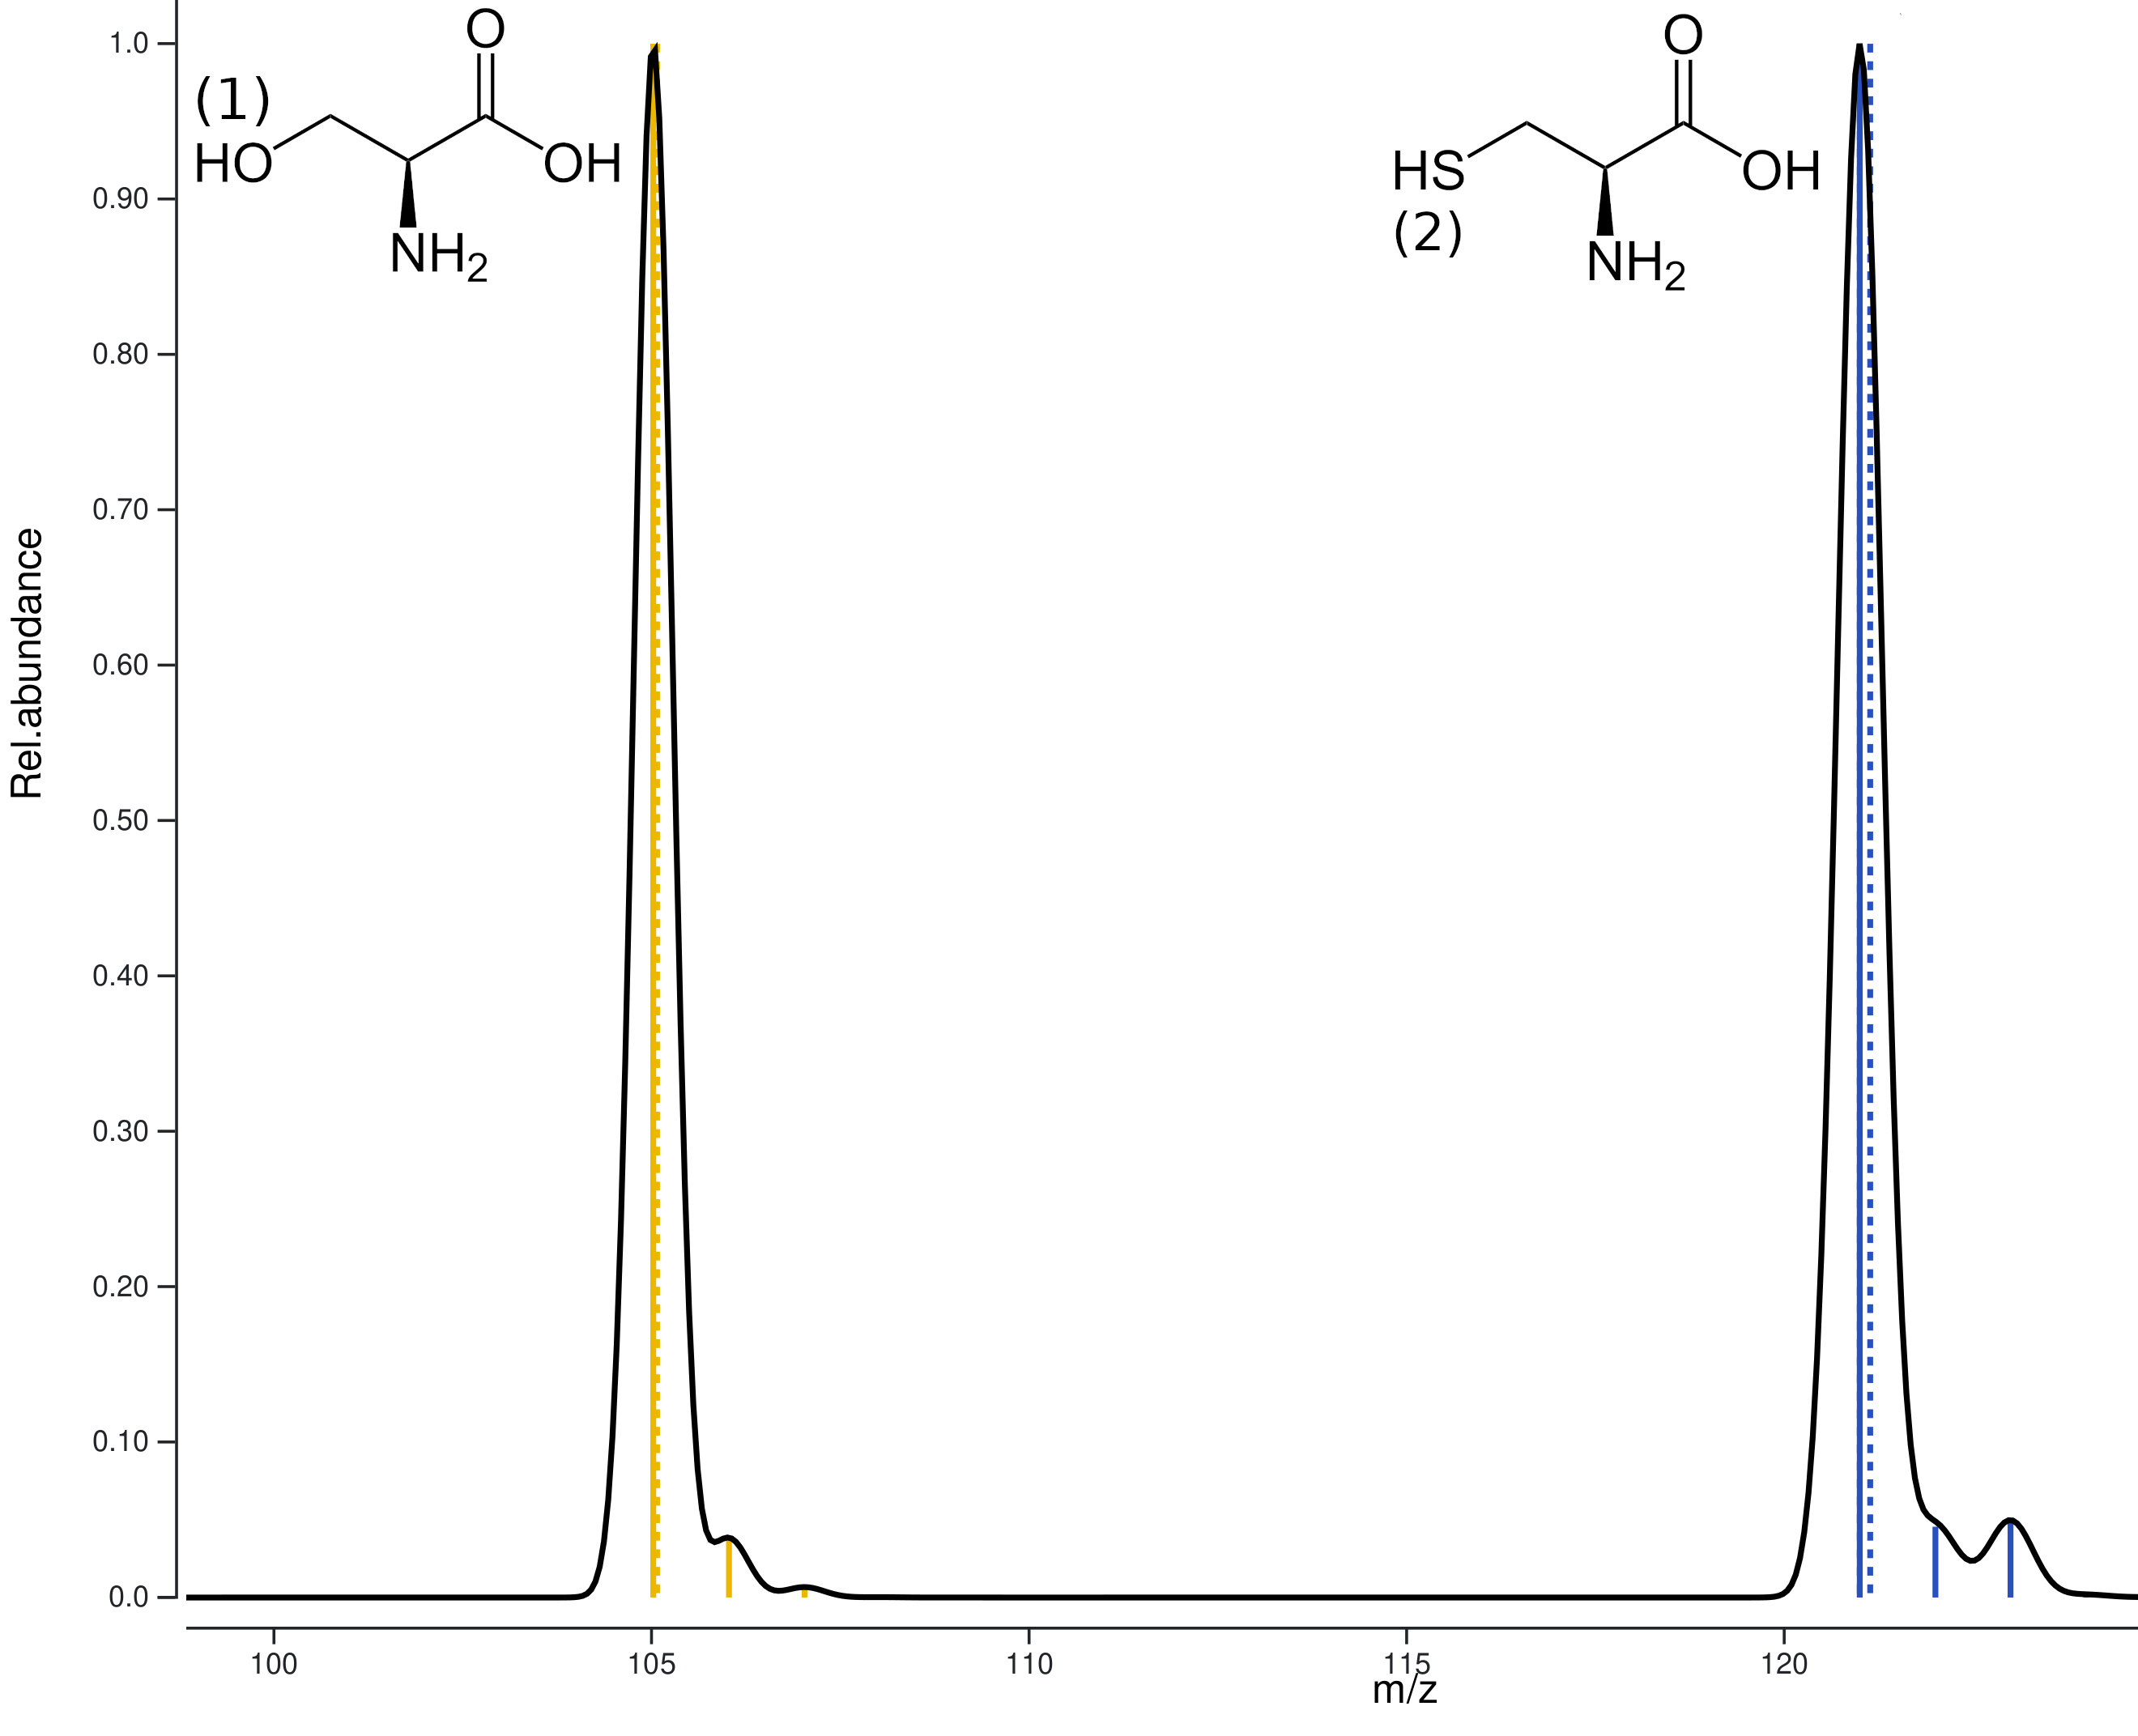
\includegraphics[width=0.75\textwidth]{./Resources/Simulated_Mass_Spectrum.png}
   \centering
   \caption{Computergeneriertes Massenspektrum von der Aminosäure \emph{Serin} (1) und \emph{Cystesin} (2). Peak von \emph{Serin} liegt bei 105; bei \emph{Systesin} um 121. y: relative Häufigkeit}
\end{figure}

Die Maxima werden \gerquot{Peaks} genannt und sind für eine Aminosäure an charakteristischer Position auf der $ x $-Achse. Obwohl sich die beiden Aminosäuren in der Abbildung \ref{fig:Sim_Mass_Spec} nur durch ein Atom unterscheiden (das linke Sauerstoffatom wurde durch ein Schwefelatom ersetzt) sind deren Massenspektren auf der $ x $-Achse weit voneinander entfernt und machen die beiden Aminosäuren dadurch sicher unterscheidbar.\\

Bei einzelnen Aminosäuren funktioniert die MS zuverlässig; bei Peptiden allerdings steht man vor dem Problem, dass das Massenspektrum unübersichtlicher wird und auch Peaks, die von Hintergrundrauschen stammen, schwerer herausgefiltert werden können. Abhilfe schafft hier die Tandem-Massenspektrometrie.

\subsection{Tandem-Massenspektrometrie (MS/MS)}\label{ss:Tandem_MS}
Bei der Tandem-Massenspektrometrie (MS/MS oder MS2) werden zwei MS Vorgänge hintereinander mit einer Probe durchgeführt. Die erste MS dient dazu Ionen aus einem bestimmten \massCharge Bereich auswählbar zu machen. Es entspricht also quasi einer Form der Filterung.

Vor der 2. MS werden die ausgewählten Reste einer Fragmentierung unterzogen. Bei einer Fragmentierung führt man Energie zu mit dem Ziel, dass die Ionen zerfallen und sog. Fragment-Ionen bilden. Diese Fragment-Ionen werden dann auf dem Massenspektrum nach der 2. MS sichtbar gemacht.

Fragment-Ionen sind kleiner als die ursprünglichen Ionen. So kann die 2. MS mit einer höheren Selektivität durchgeführt werden, welches Peaks durch Hintergrundrauschen verringert. Auch lassen sich Ionen besser identifizieren, die ein sehr ähnliches \massCharge-Verhältnis besitzen. Nach der 2. MS liegt eine Fülle an Fragment-Ionen-Peaks vor, aus denen sich die ursprünglichen Strukturinformationen ableiten lassen, da Ionen in spezifische Fragmente zerfallen \cite{Gross2013}. Zusammengefasst kann man sagen, dass das MS/MS Verfahren Ergebnisse höherer Güte erzeugt im Vergleich zur einfachen MS.

\section{De-Novo-Peptidsequenzierung mit \emph{pNovo+}}\label{s:pNovoPlusSeq}
Die \emph{pNovo+} Methode ist eine \gls{gls:DeNovo}, die mit einem \gls{gls:SpecGraph}en für die Auswertung der MS2-Spektren arbeitet und eine Erweiterung des \emph{pNovo} Verfahren darstellt \cite{pNovo}. Der Hauptansatz ist, dass zwei MS/MS Durchläufe mit jeweils verschiedenen Fragmentierungsmethoden\footnote{\emph{pNovo+} verwendet die higher energy
collisional dissociation (HCD) und die electron transfer dissociation (ETD) Fragmentierungsmethoden.} durchgeführt werden. Durch die Wahl einer anderen Fragmentierungsmethode ändert sich auch das MS2-Spektrum. Wenn nun Fragmentierungsmethoden verwendet werden, die möglichst komplementäre Spektren erzeugen, dann lässt sich durch das Zusammenführen der beiden MS2-Spektren die Qualität der Ergebnisse verbessern. Zum Beispiel lassen sich dadurch viele Peaks, die vom Hintergrundrauschen stammen, entfernen.

Für die Ermittlung der Sequenz eines Peptides wird zunächst ein Spektrums-Graph gebildet \dashAndSpace in Form eines DAG (directed acyclic graph). In diesem Graphen wird dann der längste Pfad bei gegebenen Start- und Endknoten berechnet. Die Reihenfolge der Knoten, die im längsten Pfad durchlaufen werden, stellt dann die Peptidsequenz dar.

\subsection{Vorverarbeitung der MS2-Spektren}\label{ss:Vorverarbeitung}
Bevor aus den MS2-Spektren der Spektrums-Graph gebildet werden kann, müssen die Daten vorverarbeitet werden. Für die Auswertung ist es von entscheidener Bedeutung, dass möglichst wenig Peaks verwendet werden, die vom Hintergrundrauschen stammen. Im weiteren Verlauf werden an einem exemplarischen MS2-Spektrum die Verarbeitungsschritte dargestellt.\\

Der erste Schritt ist das Verwenden des natürlichen Logarithmus der Intensitäten. Die Idee dabei ist, dass Hintergrundrauschen nicht überpriorisiert wird.

\begin{figure}[H]
   \centering
   \begin{minipage}[t]{.45\linewidth}
      \centering
      \begin{tikzpicture}[scale=\tikzScale, baseline=(current bounding box.center)]
         \draw [<->,thick] (0,\yAxisHeight) node (yaxis) [above] {\yAxisUnit}
         |- (\xAxisLength,0) node (xaxis) [right] {\xAxisUnit};
\draw[thick] (0.2, 0.0) -- (0.2, 2.3);
\draw[thick] (0.382, 0.0) -- (0.382, 1.7);
\draw[thick] (0.476, 0.0) -- (0.476, 2.7);
\draw[thick] (0.456, 0.0) -- (0.456, 1.8);
\draw[thick] (0.6859999999999999, 0.0) -- (0.6859999999999999, 2.7);
\draw[thick] (0.6839999999999999, 0.0) -- (0.6839999999999999, 1.8);
\draw[thick] (0.752, 0.0) -- (0.752, 1.1);
\draw[thick] (0.8200000000000001, 0.0) -- (0.8200000000000001, 2.2);
\draw[thick] (1.076, 0.0) -- (1.076, 1.5);
\draw[thick] (1.16, 0.0) -- (1.16, 1.9);
\draw[thick] (1.2120000000000002, 0.0) -- (1.2120000000000002, 2.0);
\draw[thick] (1.28, 0.0) -- (1.28, 1.9);
\draw[thick] (1.452, 0.0) -- (1.452, 1.3);
\draw[thick] (1.426, 0.0) -- (1.426, 1.9);
\draw[thick] (1.548, 0.0) -- (1.548, 1.9);
\draw[thick] (1.6740000000000002, 0.0) -- (1.6740000000000002, 1.5);
\draw[thick] (1.788, 0.0) -- (1.788, 2.5);
\draw[thick] (1.856, 0.0) -- (1.856, 2.3);
\draw[thick] (2.036, 0.0) -- (2.036, 1.7);
\draw[thick] (2.142, 0.0) -- (2.142, 1.6);
\draw[thick] (2.2520000000000002, 0.0) -- (2.2520000000000002, 2.0);
\draw[thick] (2.386, 0.0) -- (2.386, 1.6);
\draw[thick] (2.488, 0.0) -- (2.488, 2.9);
\draw[thick] (2.4739999999999998, 0.0) -- (2.4739999999999998, 2.7);
\draw[thick] (2.504, 0.0) -- (2.504, 2.0);
\draw[thick] (2.682, 0.0) -- (2.682, 2.0);
\draw[thick] (2.702, 0.0) -- (2.702, 2.5);
\draw[thick] (2.9259999999999997, 0.0) -- (2.9259999999999997, 2.8);
\draw[thick] (3.024, 0.0) -- (3.024, 2.4);
\draw[thick] (3.096, 0.0) -- (3.096, 1.8);
\draw[thick] (3.244, 0.0) -- (3.244, 2.6);
\draw[thick] (3.362, 0.0) -- (3.362, 1.9);
\draw[thick] (3.46, 0.0) -- (3.46, 2.3);
\draw[thick] (3.516, 0.0) -- (3.516, 1.1);
\draw[thick] (3.584, 0.0) -- (3.584, 1.8);
\draw[thick] (3.652, 0.0) -- (3.652, 2.0);
\draw[thick] (3.838, 0.0) -- (3.838, 1.5);
\draw[thick] (3.8819999999999997, 0.0) -- (3.8819999999999997, 2.6);
\draw[thick] (4.088, 0.0) -- (4.088, 2.6);
\draw[thick] (4.046, 0.0) -- (4.046, 1.1);
\draw[thick] (4.167999999999999, 0.0) -- (4.167999999999999, 2.0);
\draw[thick] (4.266, 0.0) -- (4.266, 2.4);
\draw[thick] (4.38, 0.0) -- (4.38, 1.1);
\draw[thick] (4.456, 0.0) -- (4.456, 2.2);
\draw[thick] (4.644, 0.0) -- (4.644, 2.6);
\draw[thick] (4.675999999999999, 0.0) -- (4.675999999999999, 2.5);
\draw[thick] (4.898000000000001, 0.0) -- (4.898000000000001, 1.2);
   \end{tikzpicture}%
   \end{minipage}%
   \textbf{$\rightarrow$} 
   \begin{minipage}[t]{.45\linewidth}
      \centering
      \begin{tikzpicture}[scale=\tikzScale, baseline=(current bounding box.center)]
      \draw [<->,thick] (0,\yAxisHeight) node (yaxis) [above] {\yAxisUnit}
      |- (\xAxisLength,0) node (xaxis) [right] {\xAxisUnit};
\draw[thick] (0.2, 0.0) -- (0.2, {ln(2.3)});
\draw[thick] (0.382, 0.0) -- (0.382, {ln(1.7)});
\draw[thick] (0.476, 0.0) -- (0.476, {ln(2.7)});
\draw[thick] (0.456, 0.0) -- (0.456, {ln(1.8)});
\draw[thick] (0.6859999999999999, 0.0) -- (0.6859999999999999, {ln(2.7)});
\draw[thick] (0.6839999999999999, 0.0) -- (0.6839999999999999, {ln(1.8)});
\draw[thick] (0.752, 0.0) -- (0.752, {ln(1.1)});
\draw[thick] (0.8200000000000001, 0.0) -- (0.8200000000000001, {ln(2.2)});
\draw[thick] (1.076, 0.0) -- (1.076, {ln(1.5)});
\draw[thick] (1.16, 0.0) -- (1.16, {ln(1.9)});
\draw[thick] (1.2120000000000002, 0.0) -- (1.2120000000000002, {ln(2.0)});
\draw[thick] (1.28, 0.0) -- (1.28, {ln(1.9)});
\draw[thick] (1.452, 0.0) -- (1.452, {ln(1.3)});
\draw[thick] (1.426, 0.0) -- (1.426, {ln(1.9)});
\draw[thick] (1.548, 0.0) -- (1.548, {ln(1.9)});
\draw[thick] (1.6740000000000002, 0.0) -- (1.6740000000000002, {ln(1.5)});
\draw[thick] (1.788, 0.0) -- (1.788, {ln(2.5)});
\draw[thick] (1.856, 0.0) -- (1.856, {ln(2.3)});
\draw[thick] (2.036, 0.0) -- (2.036, {ln(1.7)});
\draw[thick] (2.142, 0.0) -- (2.142, {ln(1.6)});
\draw[thick] (2.2520000000000002, 0.0) -- (2.2520000000000002, {ln(2.0)});
\draw[thick] (2.386, 0.0) -- (2.386, {ln(1.6)});
\draw[thick] (2.488, 0.0) -- (2.488, {ln(2.9)});
\draw[thick] (2.4739999999999998, 0.0) -- (2.4739999999999998, {ln(2.7)});
\draw[thick] (2.504, 0.0) -- (2.504, {ln(2.0)});
\draw[thick] (2.682, 0.0) -- (2.682, {ln(2.0)});
\draw[thick] (2.702, 0.0) -- (2.702, {ln(2.5)});
\draw[thick] (2.9259999999999997, 0.0) -- (2.9259999999999997, {ln(2.8)});
\draw[thick] (3.024, 0.0) -- (3.024, {ln(2.4)});
\draw[thick] (3.096, 0.0) -- (3.096, {ln(1.8)});
\draw[thick] (3.244, 0.0) -- (3.244, {ln(2.6)});
\draw[thick] (3.362, 0.0) -- (3.362, {ln(1.9)});
\draw[thick] (3.46, 0.0) -- (3.46, {ln(2.3)});
\draw[thick] (3.516, 0.0) -- (3.516, {ln(1.1)});
\draw[thick] (3.584, 0.0) -- (3.584, {ln(1.8)});
\draw[thick] (3.652, 0.0) -- (3.652, {ln(2.0)});
\draw[thick] (3.838, 0.0) -- (3.838, {ln(1.5)});
\draw[thick] (3.8819999999999997, 0.0) -- (3.8819999999999997, {ln(2.6)});
\draw[thick] (4.088, 0.0) -- (4.088, {ln(2.6)});
\draw[thick] (4.046, 0.0) -- (4.046, {ln(1.1)});
\draw[thick] (4.167999999999999, 0.0) -- (4.167999999999999, {ln(2.0)});
\draw[thick] (4.266, 0.0) -- (4.266, {ln(2.4)});
\draw[thick] (4.38, 0.0) -- (4.38, {ln(1.1)});
\draw[thick] (4.456, 0.0) -- (4.456, {ln(2.2)});
\draw[thick] (4.644, 0.0) -- (4.644, {ln(2.6)});
\draw[thick] (4.675999999999999, 0.0) -- (4.675999999999999, {ln(2.5)});
\draw[thick] (4.898000000000001, 0.0) -- (4.898000000000001, {ln(1.2)});
      \end{tikzpicture}
      \end{minipage}
      \caption{Anwendung des $ ln $ auf einem exemplarischen MS2-Spektrum.}
\end{figure}

Für das Verständnis des nächsten Schrittes muss man sich in Erinnerung rufen, dass eine gleiche Aminosäure keineswegs immer die gleiche Masse hat. Durch Isotope existiert eine gewisse \gerquot{Massenbandbreite} für ein und dieselbe Aminosäure. MS Systeme sind heute so genau, dass sie diese Differenzen erkennen. Dies hat den ungewollten Effekt, dass mehrere Peaks zu einer Aminosäure gehören können \cite{IsotopicDistributionMS}. Gleichzeitig können die \gerquot{Massenbandbreiten} zweier Aminosäuren sich überschneiden, sodass im ungünstigen Fall zwei Peaks kaum unterscheidbar nebeneinander liegen.\\

Eine Möglichkeit mit dieser Problematik umzugehen ist die Verwendung der monoisotopischen Masse. Die monoisotopische Masse ist die \gerquot{[...] exact mass of the most abundant naturally occurring stable isotope determined relative to the mass of 12 C, which is assigned the exact value of 12.0000.} \cite{MonoisotopicMass}. Ohne dabei jetzt tiefer ins Detail zu gehen kann man sagen, dass alle Peaks, deren Intensität mit einer möglichen monoisotopischen Masse übereinstimmen, auf jeden Fall einer Aminosäure entsprechen und (höchstwahrscheinlich)\footnote{Natürlich ist es möglich, dass das Rauschen zufällig einer monoisotopischen Masse entspricht. Die Wahrscheinlichkeit dafür ist allerdings sehr gering.} kein Hintergrundrauschen sind \cite{MassDefectMS}. Diese Peaks bekommen eine sogennante \emph{charge state}.\\

Der Algorithmus verwendet die \emph{charge state} Peaks als Ausganspunkte für weitere Berechnungen. Wenn die \massCharge Differenz zu einem anderen Peak einem Peptidfragment entspricht, dann stammt dieser Peak höchstwahrscheinlich von einem Fragment. Insgesamt werden damit die relevanten Peptidfragmente herausgeholt. Abbildung \ref{MonoisotopicMassFiltering} zeigt das Ergebnis nach den beiden zuvor genannten Schritten.

\begin{figure}[H]\label{MonoisotopicMassFiltering}
   \centering
   \begin{minipage}[t]{.45\linewidth}
      \centering
      \begin{tikzpicture}[scale=\tikzScale, baseline=(current bounding box.center)]
         \draw [<->,thick] (0,\yAxisHeight) node (yaxis) [above] {\yAxisUnit}
         |- (\xAxisLength,0) node (xaxis) [right] {\xAxisUnit};
\draw[thick] (0.2, 0.0) -- (0.2, {ln(2.3)});
\draw[color=blue!85!,opacity=.55,thick] (0.382, 0.0) -- (0.382, {ln(1.7)});
\draw[color=blue!85!,opacity=.55,thick] (0.476, 0.0) -- (0.476, {ln(2.7)});
\draw[color=magenta,thick] (0.456, 0.0) -- (0.456, {ln(1.8)});
\draw[color=blue!85!,opacity=.55,thick] (0.6859999999999999, 0.0) -- (0.6859999999999999, {ln(2.7)});
\draw[color=blue!85!,opacity=.55,thick] (0.6839999999999999, 0.0) -- (0.6839999999999999, {ln(1.8)});
\draw[thick] (0.752, 0.0) -- (0.752, {ln(1.1)});
\draw[thick] (0.8200000000000001, 0.0) -- (0.8200000000000001, {ln(2.2)});
\draw[thick] (1.076, 0.0) -- (1.076, {ln(1.5)});
\draw[thick] (1.16, 0.0) -- (1.16, {ln(1.9)});
\draw[thick] (1.2120000000000002, 0.0) -- (1.2120000000000002, {ln(2.0)});
\draw[thick] (1.28, 0.0) -- (1.28, {ln(1.9)});
\draw[color=blue!85!,opacity=.55,thick] (1.452, 0.0) -- (1.452, {ln(1.3)});
\draw[color=blue!85!,opacity=.55,thick] (1.426, 0.0) -- (1.426, {ln(1.9)});
\draw[color=magenta,thick] (1.548, 0.0) -- (1.548, {ln(1.9)});
\draw[color=blue!85!,opacity=.55,thick] (1.6740000000000002, 0.0) -- (1.6740000000000002, {ln(1.5)});
\draw[color=blue!85!,opacity=.55,thick] (1.788, 0.0) -- (1.788, {ln(2.5)});
\draw[thick] (1.856, 0.0) -- (1.856, {ln(2.3)});
\draw[thick] (2.036, 0.0) -- (2.036, {ln(1.7)});
\draw[thick] (2.142, 0.0) -- (2.142, {ln(1.6)});
\draw[thick] (2.2520000000000002, 0.0) -- (2.2520000000000002, {ln(2.0)});
\draw[thick] (2.386, 0.0) -- (2.386, {ln(1.6)});
\draw[color=blue!85!,opacity=.55,thick] (2.488, 0.0) -- (2.488, {ln(2.9)});
\draw[thick] (2.4739999999999998, 0.0) -- (2.4739999999999998, {ln(2.7)});
\draw[color=blue!85!,opacity=.55,thick] (2.504, 0.0) -- (2.504, {ln(2.0)});
\draw[color=magenta,thick] (2.682, 0.0) -- (2.682, {ln(2.0)});
\draw[color=blue!85!,opacity=.55,thick] (2.702, 0.0) -- (2.702, {ln(2.5)});
\draw[thick] (2.9259999999999997, 0.0) -- (2.9259999999999997, {ln(2.8)});
\draw[thick] (3.024, 0.0) -- (3.024, {ln(2.4)});
\draw[thick] (3.096, 0.0) -- (3.096, {ln(1.8)});
\draw[thick] (3.244, 0.0) -- (3.244, {ln(2.6)});
\draw[thick] (3.362, 0.0) -- (3.362, {ln(1.9)});
\draw[color=blue!85!,opacity=.55,thick] (3.46, 0.0) -- (3.46, {ln(2.3)});
\draw[color=blue!85!,opacity=.55,thick] (3.516, 0.0) -- (3.516, {ln(1.1)});
\draw[color=blue!85!,opacity=.55,thick] (3.584, 0.0) -- (3.584, {ln(1.8)});
\draw[color=magenta,thick] (3.652, 0.0) -- (3.652, {ln(2.0)});
\draw[color=blue!85!,opacity=.55,thick] (3.838, 0.0) -- (3.838, {ln(1.5)});
\draw[color=blue!85!,opacity=.55,thick] (3.8819999999999997, 0.0) -- (3.8819999999999997, {ln(2.6)});
\draw[thick] (4.088, 0.0) -- (4.088, {ln(2.6)});
\draw[thick] (4.046, 0.0) -- (4.046, {ln(1.1)});
\draw[thick] (4.167999999999999, 0.0) -- (4.167999999999999, {ln(2.0)});
\draw[thick] (4.266, 0.0) -- (4.266, {ln(2.4)});
\draw[color=blue!85!,opacity=.55,thick] (4.38, 0.0) -- (4.38, {ln(1.1)});
\draw[color=blue!85!,opacity=.55,thick] (4.456, 0.0) -- (4.456, {ln(2.2)});
\draw[color=magenta,thick] (4.644, 0.0) -- (4.644, {ln(2.6)});
\draw[color=blue!85!,opacity=.55,thick] (4.675999999999999, 0.0) -- (4.675999999999999, {ln(2.5)});
\draw[color=blue!85!,opacity=.55,thick] (4.898000000000001, 0.0) -- (4.898000000000001, {ln(1.2)});
   \end{tikzpicture}%
   \end{minipage}%
   \textbf{$\rightarrow$} 
   \begin{minipage}[t]{.45\linewidth}
      \centering
      \begin{tikzpicture}[scale=\tikzScale, baseline=(current bounding box.center)]
      \draw [<->,thick] (0,\yAxisHeight) node (yaxis) [above] {\yAxisUnit}
      |- (\xAxisLength,0) node (xaxis) [right] {\xAxisUnit};
\draw[color=blue!85!,opacity=.55,thick] (0.382, 0.0) -- (0.382, {ln(1.7)});
\draw[color=blue!85!,opacity=.55,thick] (0.476, 0.0) -- (0.476, {ln(2.7)});
\draw[color=magenta,thick] (0.456, 0.0) -- (0.456, {ln(1.8)});
\draw[color=blue!85!,opacity=.55,thick] (0.6859999999999999, 0.0) -- (0.6859999999999999, {ln(2.7)});
\draw[color=blue!85!,opacity=.55,thick] (0.6839999999999999, 0.0) -- (0.6839999999999999, {ln(1.8)});
\draw[color=blue!85!,opacity=.55,thick] (1.452, 0.0) -- (1.452, {ln(1.3)});
\draw[color=blue!85!,opacity=.55,thick] (1.426, 0.0) -- (1.426, {ln(1.9)});
\draw[color=magenta,thick] (1.548, 0.0) -- (1.548, {ln(1.9)});
\draw[color=blue!85!,opacity=.55,thick] (1.6740000000000002, 0.0) -- (1.6740000000000002, {ln(1.5)});
\draw[color=blue!85!,opacity=.55,thick] (1.788, 0.0) -- (1.788, {ln(2.5)});
\draw[color=blue!85!,opacity=.55,thick] (2.488, 0.0) -- (2.488, {ln(2.9)});
\draw[color=blue!85!,opacity=.55,thick] (2.504, 0.0) -- (2.504, {ln(2.0)});
\draw[color=magenta,thick] (2.682, 0.0) -- (2.682, {ln(2.0)});
\draw[color=blue!85!,opacity=.55,thick] (2.702, 0.0) -- (2.702, {ln(2.5)});
\draw[color=blue!85!,opacity=.55,thick] (3.46, 0.0) -- (3.46, {ln(2.3)});
\draw[color=blue!85!,opacity=.55,thick] (3.516, 0.0) -- (3.516, {ln(1.1)});
\draw[color=blue!85!,opacity=.55,thick] (3.584, 0.0) -- (3.584, {ln(1.8)});
\draw[color=magenta,thick] (3.652, 0.0) -- (3.652, {ln(2.0)});
\draw[color=blue!85!,opacity=.55,thick] (3.838, 0.0) -- (3.838, {ln(1.5)});
\draw[color=blue!85!,opacity=.55,thick] (3.8819999999999997, 0.0) -- (3.8819999999999997, {ln(2.6)});
\draw[color=blue!85!,opacity=.55,thick] (4.38, 0.0) -- (4.38, {ln(1.1)});
\draw[color=blue!85!,opacity=.55,thick] (4.456, 0.0) -- (4.456, {ln(2.2)});
\draw[color=magenta,thick] (4.644, 0.0) -- (4.644, {ln(2.6)});
\draw[color=blue!85!,opacity=.55,thick] (4.675999999999999, 0.0) -- (4.675999999999999, {ln(2.5)});
\draw[color=blue!85!,opacity=.55,thick] (4.898000000000001, 0.0) -- (4.898000000000001, {ln(1.2)});
      \end{tikzpicture}
      \end{minipage}
      \caption{Entfernen von Peaks, die keiner monoisotopischen Masse entsprechen oder benachbart mit einer Differenz von einem Fragment-Ion sind.}
\end{figure}

Tatsächlich ist die Verarbeitung an dieser Stelle noch etwas komplexer. So existieren auch noch sogenannte \emph{isotopic cluster}\footnote{Definition eines \emph{isotopic cluster} nach IUPAC: \gerquot{Group of peaks representing ions of the same elemental composition, but different isotopic compositions.} \cite[1556]{IUPACDefinitions}}, die gesondert verarbeitet werden. Für das grundsätzliche Prinzip ist dieses Detail allerdings weniger relevant.\\

Im letzten Vorberarbeitungsschritt werden Peaks aus einem irrelevanten \massCharge Bereich entfernt und naheliegende Peaks werden zusammengefasst, indem der Mittelwert sowol des \massCharge Wertes als auch der der Intensität besimmt wird. Üblicherweise liegt der Bereich für das Zusammenfassen bei $ +- 20 ppm $.

\begin{figure}[H]
   \centering
   \begin{minipage}[t]{.45\linewidth}
      \centering
      \begin{tikzpicture}[scale=\tikzScale, baseline=(current bounding box.center)]
         \draw [<->,thick] (0,\yAxisHeight) node (yaxis) [above] {\yAxisUnit}
         |- (\xAxisLength,0) node (xaxis) [right] {\xAxisUnit};
\draw[thick] (0.382, 0.0) -- (0.382, {ln(1.7)});
\draw[thick] (0.476, 0.0) -- (0.476, {ln(2.7)});
\draw[thick] (0.456, 0.0) -- (0.456, {ln(1.8)});
\draw[thick] (0.6859999999999999, 0.0) -- (0.6859999999999999, {ln(2.7)});
\draw[thick] (0.6839999999999999, 0.0) -- (0.6839999999999999, {ln(1.8)});
\draw[color=red,thick] (1.452, 0.0) -- (1.452, {ln(1.3)});
\draw[color=red,thick] (1.426, 0.0) -- (1.426, {ln(1.9)});
\draw[thick] (1.548, 0.0) -- (1.548, {ln(1.9)});
\draw[thick] (1.6740000000000002, 0.0) -- (1.6740000000000002, {ln(1.5)});
\draw[thick] (1.788, 0.0) -- (1.788, {ln(2.5)});
\draw[color=red,thick] (2.488, 0.0) -- (2.488, {ln(2.9)});
\draw[color=red,thick] (2.504, 0.0) -- (2.504, {ln(2.0)});
\draw[color=red,thick] (2.682, 0.0) -- (2.682, {ln(2.0)});
\draw[color=red,thick] (2.702, 0.0) -- (2.702, {ln(2.5)});
\draw[thick] (3.46, 0.0) -- (3.46, {ln(2.3)});
\draw[thick] (3.516, 0.0) -- (3.516, {ln(1.1)});
\draw[thick] (3.584, 0.0) -- (3.584, {ln(1.8)});
\draw[thick] (3.652, 0.0) -- (3.652, {ln(2.0)});
\draw[color=red,thick] (3.838, 0.0) -- (3.838, {ln(1.5)});
\draw[color=red,thick] (3.8819999999999997, 0.0) -- (3.8819999999999997, {ln(2.6)});
\draw[thick] (4.38, 0.0) -- (4.38, {ln(1.1)});
\draw[thick] (4.456, 0.0) -- (4.456, {ln(2.2)});
\draw[thick] (4.644, 0.0) -- (4.644, {ln(2.6)});
\draw[thick] (4.675999999999999, 0.0) -- (4.675999999999999, {ln(2.5)});
\draw[thick] (4.898000000000001, 0.0) -- (4.898000000000001, {ln(1.2)});

\fill[red!25!,opacity=.25] (0,0) rectangle (1,\yAxisHeight-\axisColorOffset);
         \fill[red!25!,opacity=.25] (\xAxisLength-1,0) rectangle (\xAxisLength-\axisColorOffset,\yAxisHeight-\axisColorOffset);
         \fill[green!25!,opacity=.25] (1,0) rectangle (\xAxisLength-1,\yAxisHeight-\axisColorOffset);
   \end{tikzpicture}%
   \end{minipage}%
   \textbf{$\rightarrow$} 
   \begin{minipage}[t]{.45\linewidth}
      \centering
      \begin{tikzpicture}[scale=\tikzScale, baseline=(current bounding box.center)]
      \draw [<->,thick] (0,\yAxisHeight) node (yaxis) [above] {\yAxisUnit}
      |- (\xAxisLength,0) node (xaxis) [right] {\xAxisUnit};
%\draw[color=red,thick] (1.452, 0.0) -- (1.452, {ln(1.3)});
%\draw[color=red,thick] (1.426, 0.0) -- (1.426, {ln(1.9)});
\draw[color=red,ultra thick] ({(1.452+1.426)/2}, 0.0) -- ({(1.452+1.426)/2}, {(ln(1.3)+ln(1.9))/2});

\draw[thick] (1.548, 0.0) -- (1.548, {ln(1.9)});
\draw[thick] (1.6740000000000002, 0.0) -- (1.6740000000000002, {ln(1.5)});
\draw[thick] (1.788, 0.0) -- (1.788, {ln(2.5)});

%\draw[color=red,thick] (2.488, 0.0) -- (2.488, {ln(2.9)});
%\draw[color=red,thick] (2.504, 0.0) -- (2.504, {ln(2.0)});
\draw[color=red,ultra thick] ({(2.488+2.504)/2}, 0.0) -- ({(2.488+2.504)/2}, {(ln(2.9)+ln(2.0))/2});

%\draw[color=red,thick] (2.682, 0.0) -- (2.682, {ln(2.0)});
%\draw[color=red,thick] (2.702, 0.0) -- (2.702, {ln(2.5)});
\draw[color=red,ultra thick] ({(2.682+2.702)/2}, 0.0) -- ({(2.682+2.702)/2}, {(ln(2.0+ln(2.5))/2});

\draw[thick] (3.46, 0.0) -- (3.46, {ln(2.3)});
\draw[thick] (3.516, 0.0) -- (3.516, {ln(1.1)});
\draw[thick] (3.584, 0.0) -- (3.584, {ln(1.8)});
\draw[thick] (3.652, 0.0) -- (3.652, {ln(2.0)});

%\draw[color=red,thick] (3.838, 0.0) -- (3.838, {ln(1.5)});
%\draw[color=red,thick] (3.8819999999999997, 0.0) -- (3.8819999999999997,{ln(2.6)});
\draw[color=red,ultra thick] ({(3.838+3.8819999999999997)/2}, 0.0) -- ({(3.838+3.8819999999999997)/2}, {(ln(1.5)+ln(2.6))/2});

\fill[red!25!,opacity=.25] (0,0) rectangle (1,\yAxisHeight-\axisColorOffset);
         \fill[red!25!,opacity=.25] (\xAxisLength-1,0) rectangle (\xAxisLength-\axisColorOffset,\yAxisHeight-\axisColorOffset);
         \fill[green!25!,opacity=.25] (1,0) rectangle (\xAxisLength-1,\yAxisHeight-\axisColorOffset);
      \end{tikzpicture}
      \end{minipage}
      \caption{Entfernen von Peaks aus einem irrelevanten \massCharge Bereich und zusammenfassen naheliegender Peaks. Rot markierte Peaks sind jene, die zusammengefasst werden.}
\end{figure}

\subsection{Bildung eines Spektrums-Graphen}\label{ss:BildungSpekGraph}
Der Spektrums-Graph wird aus einem vorverarbeiteten MS2-Spektrum (siehe Kapitel: \ref{ss:Vorverarbeitung}) gebildet. Im initialen Zustand werden die Peaks als Knoten interpretiert. Dazu kommt ein Start- und Endknoten. Jedem Knoten wird eine Masse zugeordet; im initialen Zustand bekommt der Startknoten die Masse 0 und der Endknoten die Masse des vorherigen Knotens minus der Masse des Wassers ($ 18,02 $). Die Masse der übrigen Knoten entsprechen ihren jeweils korrespondierenden \massCharge Wert. Die gerichteten Kanten werden zwischen einem Knotenpaar hinzugefügt, wenn die Differenz deren Masse gleich ist mit der Masse von ein oder zwei Aminosäuren.

\subsection{Identifikation der Aminosäuresequenz}
Der gebildete DAG kann mit klassischen Algorithmen, die den längsten Pfad suchen, durchlaufen werden. Bezogen auf die Graphentheorie entspricht die Ermittlung der Aminosäurensequenz dem Suchen eines bestimmten Pfades \dashAndSpace und nicht nach irgendeinem Pfad. Daher muss der Algorithmus mittels einer Breitensuche arbeiten, um alle möglichen Pfade zu bestimmen.

In aller Regel wird es mehrere Pfade geben. Bestimmte Sequenzen sind wahrscheinlicher als andere. So sind Pfade mit Kanten, die wegen der Massendifferenz von genau einer Aminosäure gebildet wurden, wahrscheinlicher \cite{pNovoPlus}. Alle Pfade bekommen mittels einer Scoring-Funktion einen Wert zugewiesen. Der Pfad mit dem höchsten Scoring-Wert ist wahrscheinlich das richtige Ergebnis. Die Scoring-Funktion berücksichtigt unter anderem wie viele Fragmente, die einer bestimmten Aminosäure zugeordet werden können, im MS2-Spektrum vorhanden sind \cite{pNovo}. Die Sequenz mit dem höchsten Scoring-Wert ist das Endergebnis.

\section{De-Novo-Peptidsequenzierung mit \emph{Open-pNovo}}\label{s:OpenpNovoSeq}
Bei Proteinen können posttranslationale Proteinmodifikationen (PTM) auftreten. PTMs sind Ereignisse, bei denen sich Änderungen im Protein einstellen \cite{Mann2003}; teilweise sind die Änderungen von einer Zelle erwünscht \dashAndSpace teilweise stammen sie aber auch zum Beispiel von unerwünschten Wechselwirkungen nebeneinanderliegenden Aminosäuren. Ein Teil dieser PTMs führen zu einer Änderung der Aminosäuresequenz. Dies ist für die \gls{gls:DeNovo} nicht weiter problematisch, da sowieso ohne eine Datenbank gearbeitet wird, sodass solche PTMs nicht einmal auffallen würden. Andere PTMs hingegen haben die Auswirkung, dass Stoffe gebildet werden, die nicht mehr zu der Gruppe der proteinogenen Aminosäuren gehören. Proteinogene Aminosäuren sind jene Aminosäuren, die für den Bau von Proteinen verwendet werden. Der Effekt ist also, dass Stoffe (oder deren Fragmente) bei einem Massenspektrum angezeigt werden, die kein Teil eines Peptids sein können. Bei der Sequenzierung von Peptidfragmenten muss dies daher berücksichtigt werden.
Wenn im weiteren Verlauf von PTMs gesprochen wird, dann sind solche gemeint, die für die \gls{gls:DeNovo} relevant sind.

Open-pNovo ist ein \gls{gls:DeNovo}sverfahren, welches auf pNovo+ Tool aufbaut und versucht die Problematik mit den PTMs zu lösen.

\subsection{PTMs im konstruierten DAG}
Die Konvertierung eines MS2-Spektrums läuft bis zum DAG analog ab wie in den Kapiteln \ref{ss:Vorverarbeitung} und \ref{ss:BildungSpekGraph} für pNovo+. Der Unterschied ist nun, dass es zwei Arten von Kanten gibt:

\begin{itemize}
   \item \gerquot{Normale} Kanten: Kanten, die gebildet werden, wie es bereits für \emph{pNovo+} gezeigt wurde. 
   \item \gerquot{Modifizierte} Kanten: Kanten, die zum Grahpen hinzugefügt werden, wenn die Massendifferenz zweier Knoten der Masse einer Aminosäure plus der Masse einer möglichen PTM-Änderung entspricht. 
\end{itemize}

Eine Liste aller PTMs in der Datenbank Unimod (sowohl relevante als auch nicht relevante) beinhaltet aktuell 1510 Einträge\footnote{Siehe: \url{https://www.ebi.ac.uk/ols/ontologies/unimod}} (Stand: 18.04.2022). Für die modifizierten Kanten gibt es insgesamt $ 1510 * 20 = 30200 $ mögliche Differenzen, wobei viele davon nicht relevante PTMs sind. Zum Vergleich: bei den normalen Kanten gibt es $ 20^2 = 400 $ mögliche Differenzen.

Die hohe Anzahl an Differenzen für modifizierte Kanten hat die Konsequenz, dass viele Knoten zufällig verbunden werden und dass dadurch die Genauigkeit der Ergebnisse abnimmt. Dieses Problem kann man durch eine geringere Liste an möglichen PTMs abfedern, allerdings mit einem Verlust  der Genauigkeit auf Seiten der PTMs. Es ist hier also eine Abwägung.

\subsection{Evaluierung von Open-pNovo}
Open-pNovo wurde sowohl auf drei realen als auch auf drei generierten Testdaten getestet. Tabelle \ref{tab:OpenPNovoResults} zeigt die Ergebnisse im Vergleich zu pNovo+ und zwei anderen Algorithmen. Die Datensätze enthielten die am häufigsten vorkommenden PTMs.

\begin{table}[H]
    \centering
    \begin{tabular}{l|c|c|c|c}
        \toprule
        \textbf{Testdatensätze} & \textbf{Open-pNovo+} & \textbf{pNovo+} & \textbf{PEAKS} & \textbf{Novor} \\
        \midrule
        Real (20259) & $76,3 \%$ & $68,5 \%$ & $65,8 \%$ & $39,9 \%$ \\
        Generiert (17877) & $77,8 \%$ & $0,6 \%$ & $0,5 \%$ & $0,2 \%$ \\
        \bottomrule
    \end{tabular}
    \newline
    \caption{Vergleich der durchschnittlichen richtigen \gls{gls:DeNovo} Peptidsequenzierungen von Open-pNovo und anderen Algorithmen \cite[650]{OpenPNovo}.}
    \label{tab:OpenPNovoResults}
\end{table}

Die enorm schlechten Ergebnisse der anderen Algorithmen bei den generierten Testdaten ist ein Nebeneffekt des Ziels bei der Testdatengenerierung. Denn diese wurden so ausgelegt, um die Grenzen von Open-pNovo+ zu ermitteln \cite[649]{OpenPNovo}. Eine Aussagekraft haben diese Ergebnisse also nicht. Allerdings auch bei realen Testdaten zeigt sich Open-pNovo als voll konkurrenzfähig gegenüber den anderen Algorithmen.

Noch besser zeigt sich Open-pNovo, wenn der Recall Wert betrachtet wird \dashAndSpace also die Anzahl an verschiedenen PSMs, die erkannt wurden. In diesem Fall ist der Abstand zu den anderen Algorithmen deutlich größer geworden.

\begin{table}[H]
    \centering
    \begin{tabular}{l|c|c|c|c}
        \toprule
        \textbf{Testdatensätze} & \textbf{Open-pNovo+} & \textbf{pNovo+} & \textbf{PEAKS} & \textbf{Novor} \\
        \midrule
        Real (5034) & $61,6 \%$ & $31,3 \%$ & $32,0 \%$ & $13,7 \%$ \\
        \bottomrule
    \end{tabular}
    \newline
    \caption{Vergleich der durchschnittlichen Recall Werte einer \gls{gls:DeNovo} Peptidsequenzierungen von Open-pNovo und anderen Algorithmen \cite[650]{OpenPNovo}.}
    \label{tab:OpenPNovoResultsRecall}
\end{table}

\subsection{Zusammenfassung}


% Die \gls{gls:DeNovo} nutzt die sogenannte \gls{gls:TMassSpek} für die Bestimmung der Peptidsequenz. Dabei wird die physikalische Eigenschaft ausgenutzt, dass jedes Atom bzw. jedes Molekül \dashAndSpace wenn es einer \gls{gls:Ionisation} unterzogen wurde \dashAndSpace ein charakteristisches \gls{gls:MassSpek} besitzt. Das \gls{gls:MassSpek} stellt also eine Art \gerquot{Fingerabdruck} eines Moleküls dar und macht dieses ermittelbar.

% U.U. eine Beispielgrafik eines Massenspektrums hinzufuegen ...

\subsubsection{\glsentrytext{gls:TMassSpek} bei größeren Molekülen}
Bei größeren Molekülen (wie einem Protein) führt die \gls{gls:Ionisation} dazu, dass das Molekül in kleinere spezifische Ionen zerfällt (sog. Fragmentierung). Die Fragmentierungsinformationen einer \gls{gls:DeNovo} sind meist unvollständig, da fehlende Daten bei einem Fragmentierungsschritt die Güte des Endergebnisses negativ beeinflusst. Dies wird insbesondere dann ein Problem, wenn unbekannte Änderungen in einer Peptidsequenz vorhanden sind.

Um dieses Problem zu verringern können unterschiedliche Techniken parallel eingesetzt werden, welche verschiedene Fragmente erzeugen und daher auch verschiedenartige \glspl{gls:MassSpek} zur Folge haben.\footnote{Konkret: Es wird sowohl das \gls{acr:HCD} als auch das \gls{acr:ETD} Verfahren angewendet.}

\subsection{Datenaufbereitung}
Typischerweise betrachtet man die sog. \gerquot{\glspl{gls:Peak}} in den \glspl{gls:MassSpek}. Jeder \gls{gls:Peak} stellt ein unterschiedliches Ion dar. Dazu kommen Messungenauigkeiten sowie Hintergrundrauschen. Durch die hohe Anzahl an möglichen Ionen kann nicht ohne weiteres differenziert werden, welcher der \glspl{gls:Peak} von welchen Ionen erzeugt wurden und welche nicht.

% Frage an Dominik: Ist hier eine einfache Auflistung an Techniken für die Datenaufbereitung besser?
Der Algorithmus für die Datenaufbereitung berechnet den natürlichen Logarithmus von den Intensitäten der \glspl{gls:Peak}, um Hintergrundrauschen und Messungenauigkeiten nicht überzupriorisieren. Zusätzlich dazu werden \glspl{gls:Peak}, die in einem Toleranzbereich nebeneinander liegen, zusammengefasst. Am Ende werden die \glspl{gls:Peak} entfernt, bei denen bekannt ist, dass es sich nicht um relevante Ionen handeln kann. (z.B. \glspl{gls:Peak} von Isotopen)

\begin{figure}[H]
   \centering
   \begin{minipage}[t]{.4\linewidth}
      \centering
      \begin{tikzpicture}[scale=\tikzScale, baseline=(current bounding box.center)]
         \draw [<->,thick] (0,2.75) node (yaxis) [above] {\yAxisUnit}
         |- (3,0) node (xaxis) [right] {\xAxisUnit};

         \draw[thick] (0.2,0) -- (0.2,1.1);
         \draw[thick] (0.3,0) -- (0.3,1.6);
         \draw[thick] (0.6,0) -- (0.6,1.7);
         \draw[thick] (0.8,0) -- (0.8,1.2);
         \draw[thick] (1.0,0) -- (1.0,1.1);

         \draw[color=red,thick] (1.2,0) -- (1.2,2.65);
         \draw[thick] (1.4,0) -- (1.4,1.4);
         \draw[thick] (1.6,0) -- (1.6,1.2);
         \draw[thick] (1.8,0) -- (1.8,1.3);
         \draw[thick] (2.0,0) -- (2.0,1.8);

         \draw[thick] (1.1,0) -- (1.1,2.0);
         \draw[color=red,thick] (0.35,0) -- (0.35,2.25);
         \draw[thick] (1.9,0) -- (1.9,1.4);
         \draw[color=red,thick] (2.2,0) -- (2.2,2.6);
         \draw[thick] (2.5,0) -- (2.5,1.25);

         \draw[thick] (2.7,0) -- (2.7,1.1);
         \foreach \x in {1,...,6}
         {
            \draw[thick] (1.2+\x*0.05,0) -- (1.2+\x*0.05,1.0+\x*0.15);
         }
      \end{tikzpicture}%
      % \subcaption{Exemplarische Rohdaten}
   \end{minipage}%
   \textbf{$\rightarrow$}
   \begin{minipage}[t]{.4\linewidth}
      \centering
      \begin{tikzpicture}[scale=\tikzScale, baseline=(current bounding box.center)]
         \draw [<->,thick] (0,2.75) node (yaxis) [above] {\yAxisUnit}
         |- (3,0) node (xaxis) [right] {\xAxisUnit};

         \draw[thick] (0.2,0) -- (0.2,{ln(1.1)});
         \draw[thick] (0.3,0) -- (0.3,{ln(1.6)});
         \draw[thick] (0.6,0) -- (0.6,{ln(1.7)});
         \draw[thick] (0.8,0) -- (0.8,{ln(1.2)});
         \draw[thick] (1.0,0) -- (1.0,{ln(1.1)});

         \draw[color=red,thick] (1.2,0) -- (1.2,{ln(2.65)});
         \draw[thick] (1.4,0) -- (1.4,{ln(1.4)});
         \draw[thick] (1.6,0) -- (1.6,{ln(1.2)});
         \draw[thick] (1.8,0) -- (1.8,{ln(1.3)});
         \draw[thick] (2.0,0) -- (2.0,{ln(1.8)});

         \draw[thick] (1.1,0) -- (1.1,{ln(2.0)});
         \draw[color=red,thick] (0.35,0) -- (0.35,{ln(2.25)});
         \draw[thick] (1.9,0) -- (1.9,{ln(1.4)});
         \draw[color=red,thick] (2.2,0) -- (2.2,{ln(2.6)});
         \draw[thick] (2.5,0) -- (2.5,{ln(1.25)});

         \draw[thick] (2.7,0) -- (2.7,{ln(1.1)});
         \foreach \x in {1,...,6}
         {%
            \draw[thick] (1.2+\x*0.05,0) -- (1.2+\x*0.05,{ln(1.0+\x*0.15)});
         }
      \end{tikzpicture}
      %\subcaption{Exemplarische Rohdaten}
   \end{minipage}
   \caption{Anwendung des $ln$ auf Rohdaten. Rote \glspl{gls:Peak} stellen hier exemplarisch fehlerhafte Daten dar, die nach dem $ln$ reduziert wurden.}
\end{figure}

\begin{figure}[H]
   \centering
   \begin{minipage}[t]{.4\linewidth}
      \centering
      \begin{tikzpicture}[scale=\tikzScale, baseline=(current bounding box.center)]
         \draw [<->,thick] (0,2.75) node (yaxis) [above] {\yAxisUnit}
         |- (3,0) node (xaxis) [right] {\xAxisUnit};

         \draw[thick] (0.2,0) -- (0.2,{ln(1.1)});
         \draw[thick] (0.3,0) -- (0.3,{ln(1.6)});
         \draw[thick] (0.6,0) -- (0.6,{ln(1.7)});
         \draw[thick] (0.8,0) -- (0.8,{ln(1.2)});
         \draw[thick] (1.0,0) -- (1.0,{ln(1.1)});

         \draw[thick] (1.2,0) -- (1.2,{ln(2.65)});
         \draw[thick] (1.4,0) -- (1.4,{ln(1.4)});
         \draw[thick] (1.6,0) -- (1.6,{ln(1.2)});
         \draw[thick] (1.8,0) -- (1.8,{ln(1.3)});
         \draw[thick] (2.0,0) -- (2.0,{ln(1.8)});

         \draw[thick] (1.1,0) -- (1.1,{ln(2.0)});
         \draw[thick] (0.35,0) -- (0.35,{ln(2.25)});
         \draw[thick] (1.9,0) -- (1.9,{ln(1.4)});
         \draw[thick] (2.2,0) -- (2.2,{ln(2.6)});
         \draw[thick] (2.5,0) -- (2.5,{ln(1.25)});

         \draw[thick] (2.7,0) -- (2.7,{ln(1.1)});
         \foreach \x in {1,...,6}
         {%
            \draw[color=red,thick] (1.2+\x*0.05,0) -- (1.2+\x*0.05,{ln(1.0+\x*0.15)});
         }

         \draw[dotted] (0.4,0) -- (0.4,2.75);
         \draw[dotted] (2.6,0) -- (2.6,2.75);
         \fill[red!25!,opacity=.25] (0,0) rectangle (0.4,2.75);
         \fill[red!25!,opacity=.25] (2.6,0) rectangle (3.0,2.75);
         \fill[green!25!,opacity=.25] (0.4,0) rectangle (2.6,2.75);
      \end{tikzpicture}
      %\subcaption{Exemplarische Rohdaten}
   \end{minipage}
   \textbf{$\rightarrow$}
   \begin{minipage}[t]{.4\linewidth}
      \centering
      \begin{tikzpicture}[scale=\tikzScale, baseline=(current bounding box.center)]
         \draw [<->,thick] (0,2.75) node (yaxis) [above] {\yAxisUnit}
         |- (3,0) node (xaxis) [right] {\xAxisUnit};

         \draw[thick] (0.6,0) -- (0.6,{ln(1.7)});
         \draw[thick] (0.8,0) -- (0.8,{ln(1.2)});
         \draw[thick] (1.0,0) -- (1.0,{ln(1.1)});

         \draw[thick] (1.2,0) -- (1.2,{ln(2.65)});
         %\draw[thick] (1.4,0) -- (1.4,{ln(1.4)});
         \draw[thick] (1.6,0) -- (1.6,{ln(1.2)});
         \draw[thick] (1.8,0) -- (1.8,{ln(1.3)});
         \draw[thick] (2.0,0) -- (2.0,{ln(1.8)});

         \draw[thick] (1.1,0) -- (1.1,{ln(2.0)});
         \draw[thick] (1.9,0) -- (1.9,{ln(1.4)});
         \draw[thick] (2.2,0) -- (2.2,{ln(2.6)});
         \draw[thick] (2.5,0) -- (2.5,{ln(1.25)});

         \draw[color=red,ultra thick] (1.2+1*0.05,0) -- (1.2+1*0.05,{ln(1.0+1*0.15)});
         \draw[color=red,ultra thick] (1.2+3*0.05,0) -- (1.2+3*0.05,{ln(1.0+3*0.15)});
         \draw[color=red,ultra thick] (1.2+5*0.05,0) -- (1.2+5*0.05,{ln(1.0+5*0.15)});

         \draw[dotted] (0.4,0) -- (0.4,2.75);
         \draw[dotted] (2.6,0) -- (2.6,2.75);
         \fill[red!25!,opacity=.25] (0,0) rectangle (0.4,2.75);
         \fill[red!25!,opacity=.25] (2.6,0) rectangle (3.0,2.75);
         \fill[green!25!,opacity=.25] (0.4,0) rectangle (2.6,2.75);
      \end{tikzpicture}
      %\subcaption{Exemplarische Rohdaten}
   \end{minipage}
   \caption{Entfernen von irrelevanten \glspl{gls:Peak} sowie zusammenfassen naheliegender \glspl{gls:Peak}. Hier symbolisieren die roten \glspl{gls:Peak} jene, die zusammengefasst werden.}
\end{figure}

% `\glsentrytext` funktioniert nicht für `\glspl`
\subsection{Konvertierung von \glspl{gls:MassSpek}}
Das Ziel der Konvertierung ist das Erzeugen eines \gls{gls:SpecGraph}en. Um von einem \gls{gls:MassSpek} zu einem \gls{gls:SpecGraph}en zu kommen, werden die \glspl{gls:Peak}, die nach der Datenaufbereitung (Siehe ...) übrig bleiben, als Knoten gewertet. Dazu kommt ein Start- und Endknoten. Jeder Knoten bekommt eine Gewichtung; diese Gewichtung entspricht der Stärke des \gls{gls:Peak}s.

\newcommand{\colorA}{white!30!green}
\newcommand{\colorB}{black!10!yellow}
\newcommand{\colorC}{white!40!red}
\newcommand{\colorD}{white!25!orange}
\newcommand{\colorE}{white!45!blue}
\newcommand{\colorF}{white!5!magenta}
\newcommand{\nodeFontSize}{\scriptsize}
\newcommand{\nodeScaleFactor}{100}
\newcommand{\round}[1]{\pgfmathprintnumber[precision=0]{#1}}
\newcommand{\rawA}{ln(1.7)}
\newcommand{\rawB}{ln(2.0)}
\newcommand{\rawC}{ln(2.65)}
\newcommand{\rawD}{ln(1.0+5*0.15)}
\newcommand{\rawE}{ln(1.85)}
\newcommand{\rawF}{ln(2.6)}
\newcommand{\valueA}{\pgfmathparse{int(\rawA*\nodeScaleFactor)}\pgfmathresult}
\newcommand{\valueB}{\pgfmathparse{int(\rawB*\nodeScaleFactor)}\pgfmathresult}
\newcommand{\valueC}{\pgfmathparse{int(\rawC*\nodeScaleFactor)}\pgfmathresult}
\newcommand{\valueD}{\pgfmathparse{int(\rawD*\nodeScaleFactor)}\pgfmathresult}
\newcommand{\valueE}{\pgfmathparse{int(\rawE*\nodeScaleFactor)}\pgfmathresult}
\newcommand{\valueF}{\pgfmathparse{int(\rawF*\nodeScaleFactor)}\pgfmathresult}

\begin{figure}[htb]
   \centering
      \begin{tikzpicture}[scale=\tikzScale*1.5, baseline=(current bounding box.center)]
         \draw [<->,thick] (0,2.75) node (yaxis) [above] {\yAxisUnit}
         |- (3,0) node (xaxis) [below] {\xAxisUnit};

         \draw[thick] (0.6,0) -- (0.6,{ln(1.7)}) node [right, rotate=90, color=\colorA] {\nodeFontSize\textbf{A} \valueA};
         \draw[thick] (0.8,0) -- (0.8,{ln(1.2)});
         \draw[thick] (1.0,0) -- (1.0,{ln(1.1)});

         \draw[thick] (1.2,0) -- (1.2,{ln(2.65)}) node [right, rotate=90,
         color=\colorC] {\nodeFontSize\textbf{C} \valueC};
         \draw[thick] (1.4,0) -- (1.4,{ln(1.4)});
         \draw[thick] (1.6,0) -- (1.6,{ln(1.2)});
         \draw[thick] (1.8,0) -- (1.8,{ln(1.3)});
         \draw[thick] (2.0,0) -- (2.0,{ln(1.8)}) node [right, rotate=90, color=\colorE] {\nodeFontSize\textbf{E} \valueE};

         \draw[thick] (1.025,0) -- (1.025,{ln(2.0)}) node [right, rotate=90, color=\colorB] {\nodeFontSize\textbf{B} \valueB};
         \draw[thick] (1.9,0) -- (1.9,{ln(1.4)});
         \draw[thick] (2.2,0) -- (2.2,{ln(2.6)}) node [right, rotate=90, color=\colorF] {\nodeFontSize\textbf{F} \valueF};
         \draw[thick] (2.5,0) -- (2.5,{ln(1.25)});

         \draw[thick] (1.2+1*0.05,0) -- (1.2+1*0.05,{ln(1.0+1*0.15)});
         \draw[thick] (1.2+3*0.05,0) -- (1.2+3*0.05,{ln(1.0+3*0.15)});
         \draw[thick] (1.2+5*0.05,0) -- (1.2+5*0.05,{ln(1.0+5*0.15)}) node [right, rotate=90, color=\colorD] {\nodeFontSize\textbf{D} \valueD};
      \end{tikzpicture}
      \caption{Ausgewählte \glspl{gls:Peak} mit einem exemplarischen x Wert.}
\end{figure}

\newcommand{\modVal}{4}

Gerichtete Kanten zwischen den Knoten werden ausgebildet, wenn diese eine Differenz von genau einer oder zwei Aminosäurereste\footnote{Da eine Aminosäure vielerlei an Reste besitzen kann, ergeben sich mehr als 40 Differenzen, die diese Bedingung erfüllen.} besitzen. Der Einfachheit halber wird im folgenden eine Kante ausgebildet, wenn die Differenz genau \textbf{\modVal} \space beträgt.

% Um einzele Knotennamen einzufärben: \textcolor{\colorA}{A}
\newcommand{\findRaw}[1]{\csname raw#1\endcsname}
\newcommand{\findValue}[1]{\csname value#1\endcsname}
\newcommand{\findColor}[1]{\csname color#1\endcsname}
\newcommand{\cmark}{\ding{51}}
\newcommand{\xmark}{\ding{55}}
\newcommand{\tableRow}[2]
{%
   % Welche Zeile soll farblich hinterlegt werden ?
   \pgfmathparse{Mod(abs(int(\findRaw{#1}*\nodeScaleFactor) - int(\findRaw{#2}*\nodeScaleFactor)),\modVal)}
   \pgfmathtruncatemacro\myresult{\pgfmathresult==0.0?1:0}
   %\ifthenelse{\myresult=1}{A}{B}
   \ifnum\myresult=1 A \else B \fi

   (#1,#2) &
   \findValue{#1} &
   \findValue{#2} &
   \pgfmathparse{abs(int(\findRaw{#1}*\nodeScaleFactor) - int(\findRaw{#2}*\nodeScaleFactor))}\round{\pgfmathresult} &

   % Hilfreiche Infos für das Erstellen von Ausdrücken: https://tikz.dev/math-parsing
   \pgfmathparse{Mod(abs(int(\findRaw{#1}*\nodeScaleFactor) - int(\findRaw{#2}*\nodeScaleFactor)),\modVal)}
   % https://www.reddit.com/r/LaTeX/comments/57ck5p/tikz_which_conditionals_to_use_to_compare_numbers/
   \pgfmathtruncatemacro\myresult{\pgfmathresult==0.0?1:0}
   \round{\pgfmathresult}
   \ifthenelse{\myresult=1}{\cmark}{\xmark}
   \\
}
% Hilfestellung: https://tex.stackexchange.com/questions/604496/how-to-generate-beautiful-tables-in-latex
\begin{table}[H]
    \centering
    \begin{tabular}{lllcc}
        \toprule
        \thead{\textbf{$\mathbf{(u,v)}$}} & \thead{$\mathbf{u}$} & \thead{$\mathbf{v}$} & \thead{$\mathbf{\Delta(u,v)}$} & \thead{$\Delta(u,v)\bmod\modVal$}\\
        \midrule
        \tableRow{A}{B}
        \tableRow{A}{C}
        \tableRow{A}{D}
        \tableRow{A}{E}
        \tableRow{A}{F}
        \tableRow{B}{C}
        \tableRow{B}{D}
        \tableRow{B}{E}
        \tableRow{B}{F}
        \tableRow{C}{D}
        \tableRow{C}{E}
        \tableRow{C}{F}
        \tableRow{D}{E}
        \tableRow{D}{F}
        \tableRow{E}{F}
        \bottomrule
    \end{tabular}
    \caption{Bestimmung der Kanten}
\end{table}

Darstellung der Daten als gewichteter, gerichteter azyklischer Graph. Zusätzlich benötigt der Graph noch separate Start- und Zielknoten; diese sind für die späteren Berechnungen unerlässlich.

\newcommand{\printVertices}[2]%
{%
   \Vertex[x=-8,y=0]{Start}
   \Vertex[x=8,y=0]{End}
   \foreach \x [count=\xi] in {#1}
   {%
      \foreach \y [count=\yi] in {#2}
      {%
         \ifthenelse{\xi=\yi}{
         \tikzstyle{VertexStyle}=[shape=circle,fill=\y,draw=black,line width=0.75pt]
         \Vertex[x=-7+\xi*2,y=0]{\x}}{\break}
      }
   }
}
% https://tex.stackexchange.com/questions/245448/adjusting-edge-and-vertex-label
\begin{figure}[htb]
   \centering
   \begin{tikzpicture}[scale=0.75,transform shape]
      \tikzstyle{VertexStyle}=[shape=circle,fill=white,draw=black,line width=1pt]

      \printVertices{A,B,C,D,E,F}{\colorA, \colorB, \colorC, \colorD, \colorE, \colorF}

      \tikzstyle{LabelStyle}=[fill=white, sloped]
      \tikzstyle{EdgeStyle}=[bend left, post]
      \Edge[label=$0$](Start)(A)
      \Edge[label=$0$](F)(End)
      \tikzstyle{EdgeStyle}=[bend right, post]
      \Edge[label=$16$](A)(B)
      \tikzstyle{EdgeStyle}=[bend left, post]
      \Edge[label=$44$](A)(C)
      \Edge[label=$8$](A)(E)
      \tikzstyle{EdgeStyle}=[bend right, post]
      \Edge[label=$28$](B)(C)
      \Edge[label=$8$](B)(E)
      \Edge[label=$36$](C)(E)
      \tikzstyle{EdgeStyle}=[bend left, post]
      \Edge[label=$40$](D)(F)
   \end{tikzpicture}
   \caption{Erzeugter DAG}
\end{figure}

Bereits an diesem Minimalbeispiel ist zu erkennen, dass die gebildeten Knoten in einem \glspl{gls:SpecGraph} nur wenige ausgehende Kanten besitzen. Dies ist nicht dem Beispiel geschuldet sondern ist tatsächlich auch in der Praxis der Regelfall. Dies ist eine hilfreiche Beobachtung für die Datenauswertung (siehe Abschnitt~\ref{Datenauswertung} \gerquot{\titleref{Datenauswertung}}).


\subsection{Datenauswertung}\label{Datenauswertung}
Um nun aus dem Graphen die Peptidsequenz zu gewinnen müssen alle längsten Pfade im DAG gefunden werden. Da die Kanten gewichtet sind, kann es durchaus mehrere längste Pfade geben. Gleichwohl es Algorithmen für das Problem des längsten Pfades in einem Graphen gibt, handelt es sich hierbei um ein $NP$-schweres Problem. Es existiert also (wahrscheinlich) kein effizienter Algorithmus. Erschwerend kommt hinzu, dass der Graph nicht zwingend ein zusammenhängender Graph sein muss \dashAndSpace auch wenn dies meist der Fall ist. Der Graph muss daher vor Berechnungsbeginn auf diese Eigenschaft hin überprüft werden.

Im Falle der \glspl{gls:SpecGraph} existiert die Eigenschaft, dass solche Graphen meist eine geringe Dichte an Kanten aufweisen. Dies hat den positiven Effekt, dass die Anzahl an überhaupt möglichen längsten Pfaden recht gering ist. Zusätzlich dazu kann die Warteschlange, die in den longest Path DAG Algorithmen verwendet werden, angepasst werden. Da die Gewichtung der Kanten als eine Art \gerquot{Wahrscheinlichkeit}, dass die nächste Kante die reale Peptidsequenz darstellt, interpretiert werden kann, kann eine priorisierte Warteschlange verwendet werden, die die Laufzeit ebenfalls verbessert. In Summe führen diese Eigenschaften der \glspl{gls:SpecGraph} dazu, dass das längste Pfade Problem in solchen Fällen auf die Laufzeit $\mathcal{O}(abs(E) + log(d))$ reduziert werden kann.\\

Zusammengefasst: Es wird versucht die speziellen Eigenschaften der Graphen auszunutzen, um die Laufzeit zu verbessern.


\section{Ergebnisse/Evaluierung}
Im folgenden Kapitel werden die Probleme, die in der Praxis bei der Verwendung des Verfahrens auftreten, erläutert und mögliche Lösungsansätze aufgezeigt.

\subsection{Probleme in der Praxis}
\subsubsection{Qualität der Messwerte}
Obwohl eine Datenaufbereitung stattfindet, ist das Verfahren bei der Verwendung von \glspl{gls:SpecGraph} stark auf die Genauigkeit der Messwerte angewiesen. Zwar sind durch technische Fortschritte bei der \gls{gls:TMassSpek} die Daten hochwertiger geworden; dennoch gestaltet sich das Sequenzieren von unbekannten Peptidsequenzen als schwierig. Mit heutigen Gerätschaften lassen sich bei der Verwendung des genannten Verfahrens bis zu 13 Peptide mit einer durchschnittlichen Genauigkeit von 94\% ermitteln. Danach nimmt diese sprunghaft ab. Für brauchbare Ergebnisse wird \dashAndSpace je nach Literatur \dashAndSpace eine Trefferquote von 90-95\% vorausgesetzt.
\subsubsection{Fehlende Betrachtung der \glsentrytext{gls:StereoIsomerie}}\label{FehlendeStereoInfos}
Das komplette Verfahren basiert auf das Masse-Ladungs-Verhältnis, sodass Stereoinformationen schlicht nicht ermittelt werden können. Es kann zwar mithilfe einer energetischen Betrachtung bestimmt werden welche \glspl{gls:StereoIsomer} in welchen Verhältnis auftreten (müssten). Dabei handelt es sich allerdings lediglich um eine grobe Abschätzung.
\subsubsection{Identifikation der Aminosäuren über Massendifferenz}
Die Grundidee bei der Identifikation von Aminosäuren ist die Betrachtung der Massendifferenzen zwischen zwei \glspl{gls:Peak}. Zwar liefert dieser Ansatz häufig passende Ergebnisse. Dennoch ist solch eine Differenz nicht in der Lage jede Aminosäure immer eindeutig zu identifizieren, da bestimmte Kombinationen (fast) gleiche Differenzen besitzen. Der Algorithmus, der die Gewichtungen bestimmt, arbeitet nur mit ganzzahligen Werten. Dadurch gehen leichte Unterschiede, die durch die Isotope (insb. die des Kohlenstoffes) begründet sind, meist durch die Float Integer Konvertierung verloren.

\subsection{Lösungsansätze}
\subsubsection{Verbesserung der Ergebnisse durch Machine Learning}
Bei der Sequenzierung werden ab einer gewissen Länge unweigerlich Fehler eintreten.\cite[S.621,Figure 5]{pNovoPlus} Dadurch, dass nicht jede Peptidsequenz gleich wahrscheinlich ist\footnote{Dies ist u.a. dadurch begründet, dass die Reste der Aminosäuren sich gegenseitig beeinflussen (können), sodass bestimmte Sequenzen energetisch ungünstig sind und lediglich vermindert auftreten.}, können mittels Machine Learning grundsätzlich die Ergebnisse verbessert werden. insbesondere dann, wenn die ermittelte Differenz keinen eindeutigen Rückschluss auf die Aminosäure zulässt.

\section{Zusammenfassung}
Im letzten Kapitel werden die ungelösten Probleme genannt und erklärt warum diese eine Relevanz für die Praxis haben. Am Ende findet eine kritische Betrachtung des Verfahrens im allgemeinen statt.

\subsection{Ungelöste Probleme}
Wie bereits in \ref{FehlendeStereoInfos} erwähnt, kann das Verfahren designbedingt keine Stereoinformationen ermitteln. Daher ist es in diesem Fall besonders wichtig abzuschätzen, ob das Fehlen dieser Informationen tatsächlich eine Relevanz hat. Wenn nur die Peptidsequenz betrachtet werden soll, dann stellt dies kein Problem dar. Aber sobald jedweige Abschätzungen anhand der ermittelten Sequenz stattfinden soll, dann kann das Fehlen jener Informationen zu massiven Fehlern führen.\\

Wenn für die Verbesserung der Ergebnisse Machine Learning in Betracht kommt, dann muss dabei berücksichtigt werden, dass dadurch unter Umständen einer der großen Vorteile der \gls{gls:DeNovo} verloren geht \dashAndSpace und zwar dass keine Vorinformationen für die Sequenzierung notwendig sind. Hierbei kommt es auf den konkreten Anwendungsfall an, ob das Verlieren dieser Eigenschaft eine Bedeutung besitzt.

\subsection{Kritische Betrachtung}
Die \gls{gls:DeNovo} mit der Unterstützung von \glspl{gls:SpecGraph} stellt eine Möglichkeit dar Polypeptide mit bis zu einer Länge von etwa 12 Peptiden ausreichend zuverlässig zu bestimmen. Die Autoren des Papers \cite{OpenPNovo} haben die Software frei zur Verfügung gestellt, sodass sie in jedem Fall ein Blick wert ist.
Gegenüber anderen Ansätzen ist das Verfahren zwar konkurrenzfähig, allerdings nicht immer die beste Wahl \cite[650]{OpenPNovo}. Die Grundidee mittels der Massendifferenz auf die Aminosäuren zu schließen wird nie fehlerfrei sein, sodass dieses Verfahren weniger die bereits vorhandenen Systeme ersetzten kann, sondern eher ein weiteres Werkzeug für die \gls{gls:DeNovo} darstellt.

\begingroup
\setlength{\emergencystretch}{.5em}
\printbibliography
\endgroup

\end{document}
%%%%% %%%%% %%%%% %%%%% %%%%% \end{document} %%%%% %%%%% %%%%% %%%%% %%%%%

\PassOptionsToPackage{table}{xcolor}
\documentclass[a4paper, 12pt]{article}
\usepackage[utf8]{inputenc} % UTF-8 Kodierung verwenden
\usepackage[backend=biber, sorting=none]{biblatex}
\addbibresource{P2_De-Novo-Sequencing using Spectrum-Graphs.bib}
\usepackage[total={6.5in, 9in}]{geometry}
% \usepackage[onehalfspacing]{setspace} % 1.5 Spacing
\usepackage[singlespacing]{setspace} % 1 Spacing
\usepackage[T1]{fontenc}    % Fonts mit westeuropäischer Codierung verwenden
\usepackage[ngerman]{babel} % Neue deutsche Sprache
\usepackage{csquotes}
\usepackage{fancyhdr}       % Kopf- und Fusszeilen
\usepackage{tikz}           % Fuer das Erstellen von einfachen Grafiken
\usepackage{tkz-berge}
\usepackage{pifont}
\usepackage{makecell}
\usepackage{titleref}
\usepackage{booktabs}
\usepackage{float}          % Fuer den Positionierungsbefehl '[H]'
\usepackage{fancyhdr}       % Angepasste Header und Footer
\usepackage{titling}        % Fuer Befehle wie \thetitle
% \usepackage{showframe}     % Boxen mit Rand visualisieren (nur für das Schreiben des Dokuments brauchbar!)
\usepackage{translator}
\usepackage{subcaption}
\usepackage{caption}
\usepackage[
nonumberlist, %keine Seitenzahlen anzeigen
%acronym,      %ein Abkürzungsverzeichnis erstellen
toc,          %Einträge im Inhaltsverzeichnis
section,      %im Inhaltsverzeichnis auf section-Ebene erscheinen
nopostdot     %Den Punkt am Ende jeder Beschreibung deaktivieren
]{glossaries}
\makenoidxglossaries

% \setlength{\abovecaptionskip}{1ex}
% \setlength{\belowcaptionskip}{1ex}
\setlength{\floatsep}{24pt}
\setlength{\textfloatsep}{24pt}
\setlength{\headheight}{15pt}

\setcounter{tocdepth}{1}

\title{De-Novo-Sequencing using Spectrum-Graphs, enabling Open Searches}
\author{Dominik Habermann}
\date{\today}

% Kopf- und Fussnoten anpassen
\pagestyle{fancy}
\fancyhf{}
\fancyhead[L]{\thetitle}
%\fancyhead[R]{\thetitle}
\fancyfoot[C]{\thepage}


% Glossar- und Abkürzungsverzeichnis
\input{./Resources/P2_De-Novo-Sequencing using Spectrum-Graphs.gls}
\input{./Resources/P2_De-Novo-Sequencing using Spectrum-Graphs.acr}

\newcommand{\gerquot}[1]{\glqq#1\grqq}
\newcommand{\dashAndSpace}{\textendash \space}
\newcommand{\dashAndSpaceSeq}[1]{\dashAndSpace#1 \dashAndSpace}
\newcommand{\tikzScale}{1.0}
\newcommand{\massCharge}{$ m/z $ }
\newcommand{\xAxisUnit}{\massCharge}
\newcommand{\yAxisUnit}{$y$}
\newcommand{\yAxisHeight}{3}
\newcommand{\xAxisLength}{5}
\newcommand{\axisColorOffset}{0.15}

\renewcommand{\floatpagefraction}{0.8}
% Workaround um die Überschrift des Glossars anzupassen
% Siehe: https://tex.stackexchange.com/questions/426390/how-can-i-rename-the-header-titles-of-the-glossary
\addto\captionsngerman
{%
    \renewcommand*{\glossaryname}{Begriffserklärungen}%
}
  


%%%%% %%%%% %%%%% %%%%% %%%%% \begin{document} %%%%% %%%%% %%%%% %%%%% %%%%%
\begin{document}

\maketitle

\section{Einleitung}\label{s:Einleitung}
\subsection{Biomedizinische Fragestellung}
Peptide sind organische Verbindungen von miteinander verknüpften Aminosäuren. Bei der Sequenzierung von Peptiden versucht man die Aminosäuresequenz \dashAndSpaceSeq{also die Abfolge an vorhandenen Aminosäuren} zu bestimmen. Das Wissen über die Aminosäuresequenz ist von großer Bedeutung für den Forschungsbereich der Proteomik. Die Proteomik beschäftigt sich mit der Erforschung von Proteinen. Dies beinhaltet unter anderem auch die Analyse von Enzymen.

Da es 20 verschiedene Aminosäuren gibt \cite{rudat2021alanins}, die weitesgehend beliebig miteinander kombiniert werden können, existiert eine stark wachsende Anzahl an möglichen Variationen (oder Kombinationen(!)). Die Regeln der Kombinatik liefert uns hierfür die Formel $ f(x)=20^x $ wobei $ x $ hier die Anzahl an Aminosäuren ist. Es ist direkt erkennbar, dass selbst bei einer geringen Peptidlänge die Anzahl an möglichen Sequenzen eine Größenordnung erreicht, die von Computersystemen nicht mehr verarbeitet werden kann. Zum Vergleich: Proteine können aus wenigen Hundert bis hin zu aus mehreren Zehntausend Aminosäuren bestehen. Die Frage, die sich hier stellt: \emph{Ist es zumindest für kurze Peptide mögich diese sicher zu sequenzieren?}

\subsection{Methoden der Aminosäuresequenzierung}
Das Ziel der verschiedenen Sequenzierungsverfahren ist eine möglichst exakte Bestimmung der Aminosäuresequenz. Alle Sequenzierungsverfahren arbeiten mit der Massenspektrometrie (MS). Dabei handelt es sich um ein Verfahren, welches chemische Verbindungen identifizieren kann (eine genauere Erklärung folgt in Kapitel \ref{s:MS}). Viele Analysen arbeiten mit dem Ansatz, dass die Ergebnisse einer MS \dashAndSpaceSeq{genannt wird es Massenspektrum} mit einer Datenbank verglichen werden. Wenn die chemische Verbindung bereits einmal indentifiziert wurde, dann wird sich ein Eintrag in der Datenbank finden lassen.

Die hier vorgestellten Methoden \emph{pNovo+} und \emph{Open-pNovo} gehören zur Gruppe der \gls{gls:DeNovo}en. Im Gegensatz zu anderen Verfahren werden hierbei keinerlei Daten aus Datenbanken verwendet. Stattdessen findet eine Tandem-Massenspektrometrie Anwendung. Bei dieser Form der MS werden zwei MS Durchgänge hintereinander durchgeführt, wobei nach dem ersten Vorgang ein Teil der Probe isoliert wird und vor der 2. MS \gerquot{fragmentiert} wird (hierzu eine Beschreibung in Kapitel \ref{ss:Tandem_MS} mit mehr Details). Die \gls{gls:DeNovo} hat den bedeutsamen Vorteil, dass auch Peptide sequenziert werden können zu denen es keine oder nur unvollständige Informationen gibt.

% Im ersten Kapitel findet zu Beginn eine Erklärung der wichtigsten Begriffe und Abkürzungen statt. Dazu wird eine Themenabgrenzung durchgeführt sowie die Ausgangssituation beschrieben.

% \printnoidxglossaries

%\subsection{Themenabgrenzung}
%Folgende Aspekte sind Bestandteil dieser Ausarbeitung:
%\begin{itemize}
%   \item Was ist die \gls{gls:DeNovo}?
%   \item Was erhofft man sich von dieser Technologie?
%   \item Welche Probleme liegen vor, die von der Seite der Informatik %gelöst / verbessert werden können?
%   \item Inwiefern spielen die Spektrums-Graphen dabei eine Rolle?
%\end{itemize}


% In diesem Abschnitt werden die relevanten Herangehensweisen sowohl für die Datengewinnung als auch für deren Auswertung erklärt.

\section{Massenspektrometrie (MS)}\label{s:MS}
Wie bereits in Kapitel \ref{s:Einleitung} erwähnt, wird die MS verwendet, um chemische Strukturen zu identifizieren. Moderne Ansätze der MS wurden zu Beginn des 20. Jahrhunderts entwickelt \cite{griffiths2008brief}. Seitdem gab es etliche Erweiterungen; das Grundprinzip ist dennoch immer gleich geblieben. Grob vereinfacht besteht eine MS aus folgenden vier Schritten:

\begin{itemize}
   \item \textbf{Ionisation}: Die Moleküle in der Probe bekommen eine positive oder negativ Ladung
   \item \textbf{Überführung in Gasphase}: Durch Energie wird die Probe in die Gasphase überführt
   \item \textbf{Anlegen eines elektrischen Feldes}: Die Ionen werden durch das elektrische Feld beschleunigt
   \item \textbf{Massenanalyse}: Ionen werden anhand des Masse-Ladungs-Verhältnisses \gerquot{sortiert}
\end{itemize}

Für die Schritte gibt es verschiedene Verfahren, wobei die Unterschiede hier nicht relevant sind. Jedes dieser Verfahren nutzt die physikalische Eigenschaft aus, dass Ionen in einem Magnetfeld in Abhänigkeit ihres Verhältnisses zwischen ihrer Masse und ihrer Ladung (häufig abgekürzt mit \massCharge) unterschiedlich reagieren. So wird bei der MS nicht die Masse gemessen \dashAndSpaceSeq{auch wenn der Name es vermuten lässt} sondern die Ionenhäufigkeit bei einem bestimmten \massCharge Verhältnis. Diese Häufigkeit wird dann in einem Massenspektrum graphisch dargestellt \cite{Glish2003}. Abbildung \ref{fig:Sim_Mass_Spec} zeigt ein computergeneriertes Massenspektrum von zwei ähnlichen Aminosäuren.

% Grafik generiert von der Website: https://www.protpi.ch/Calculator/MassSpecSimulator
\begin{figure}[H]
   \label{fig:Sim_Mass_Spec}
   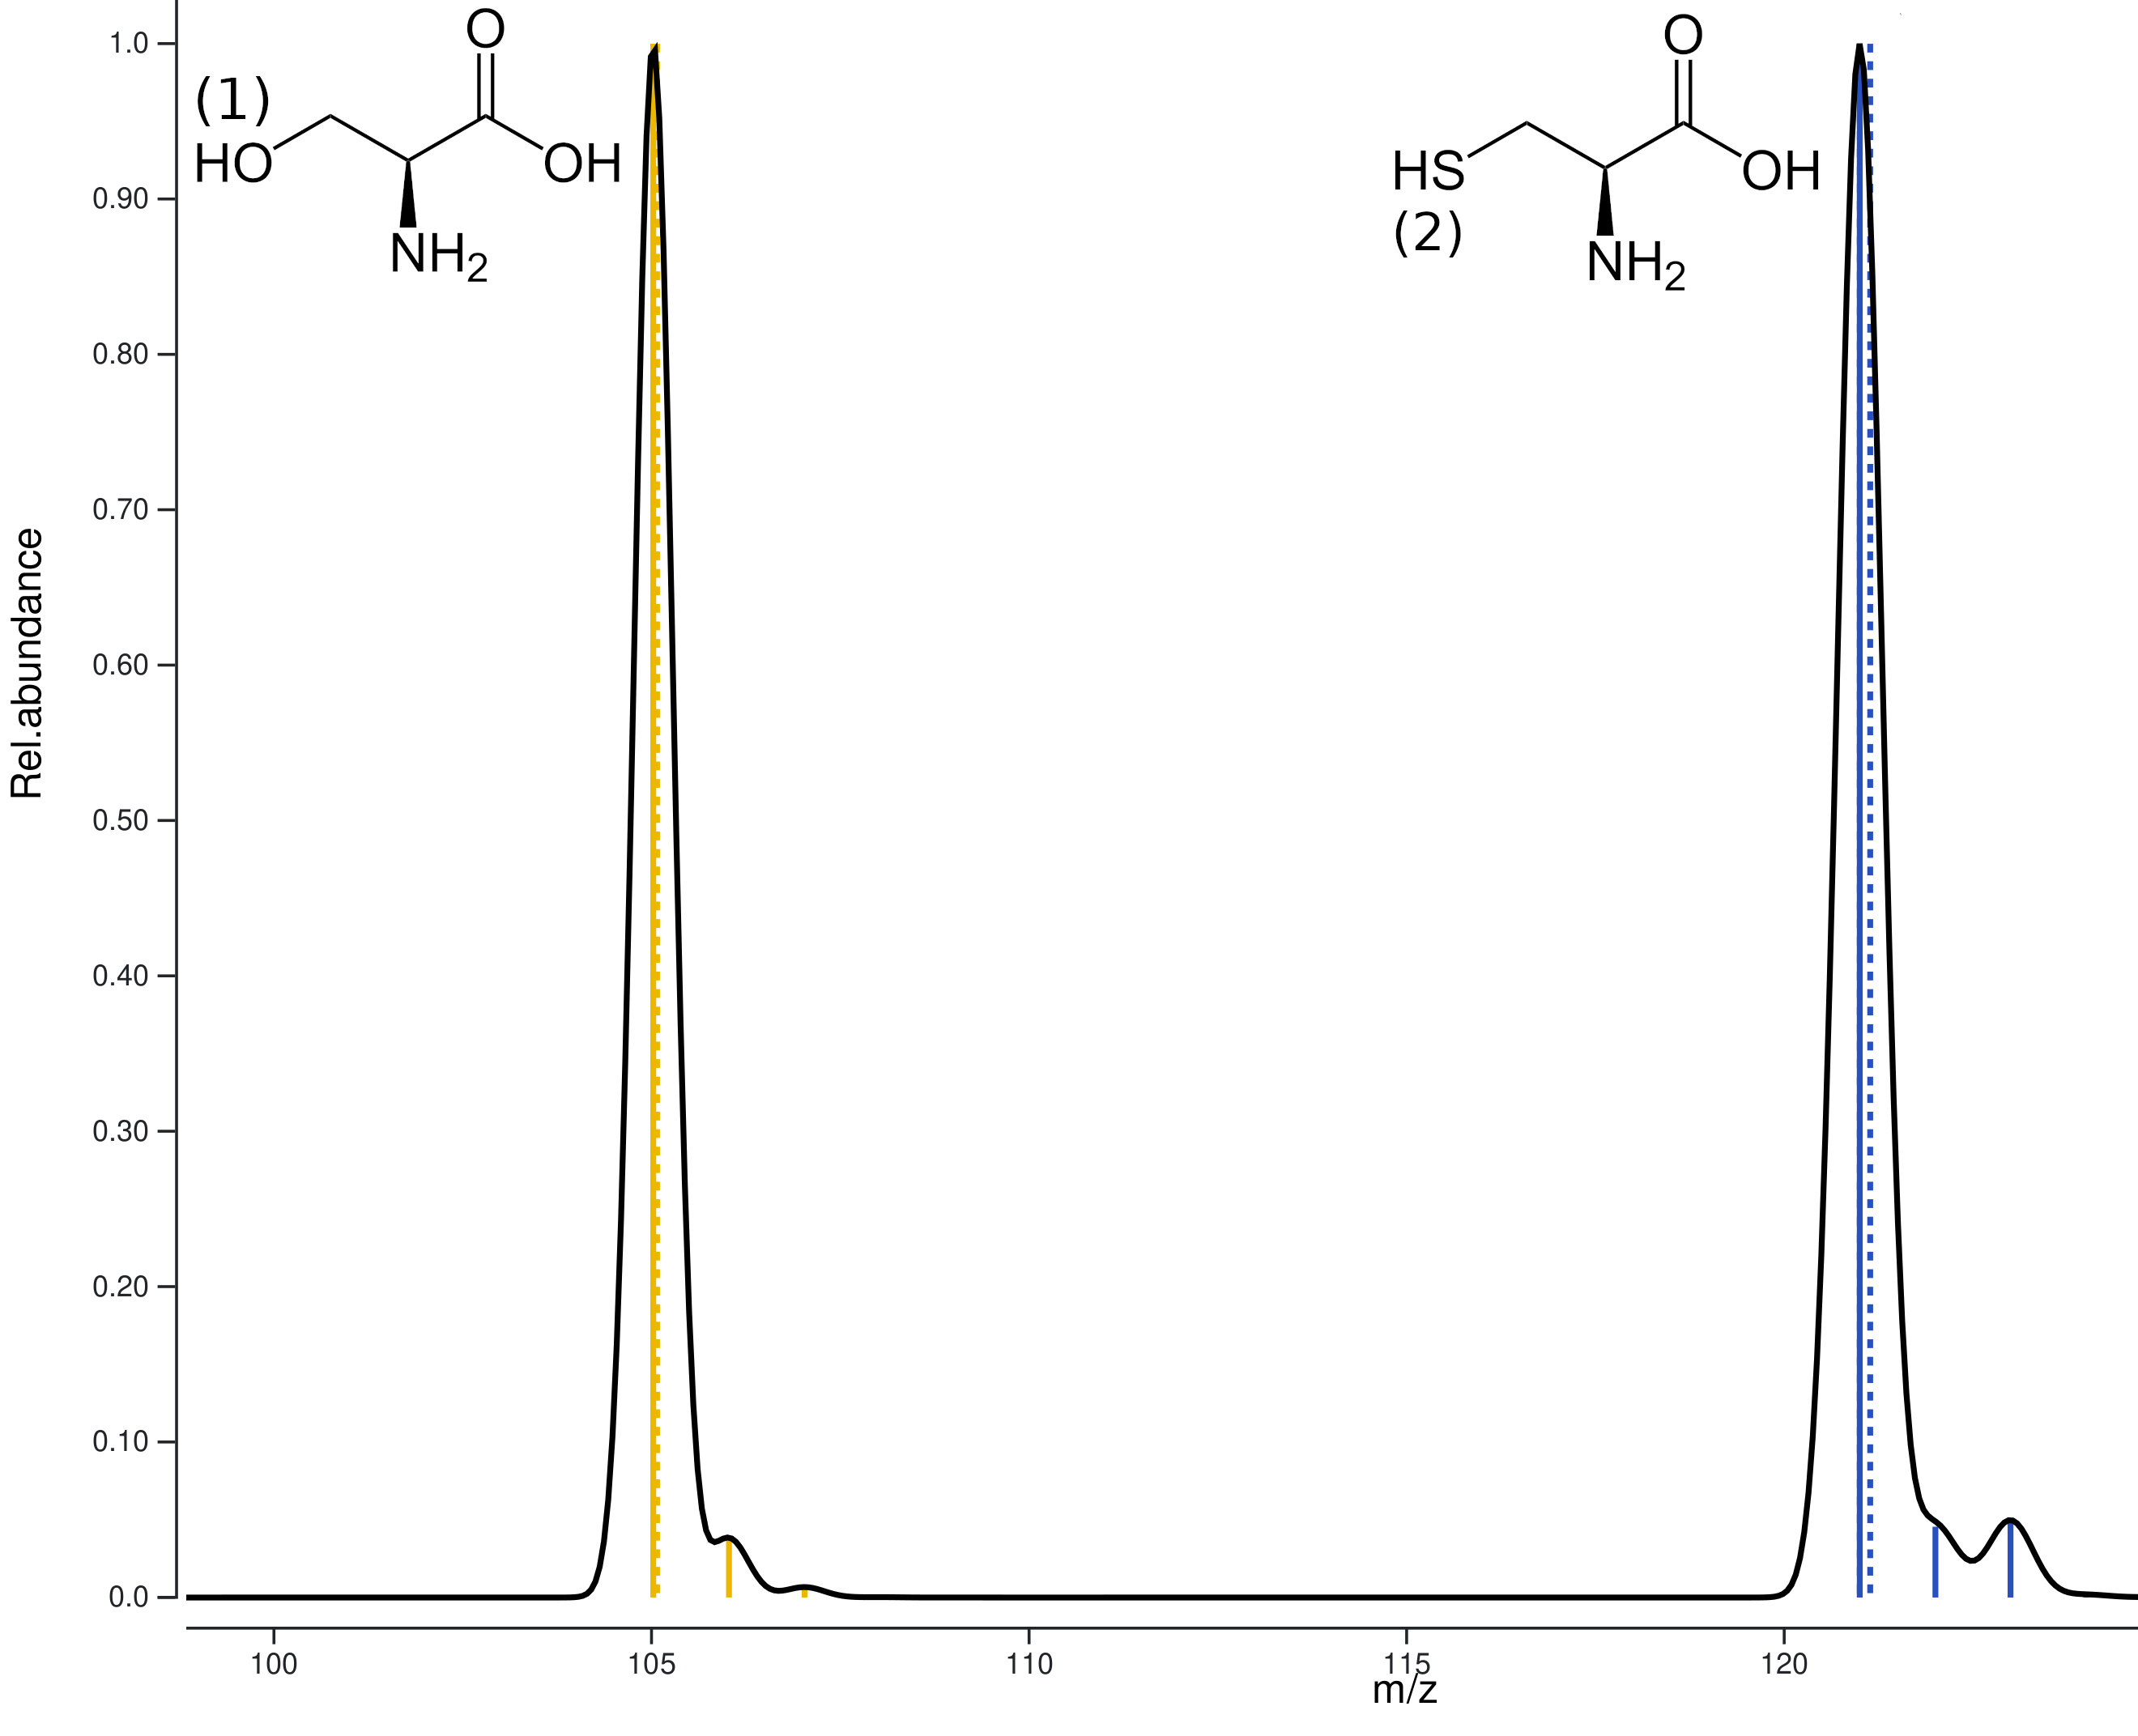
\includegraphics[width=0.75\textwidth]{./Resources/Simulated_Mass_Spectrum.png}
   \centering
   \caption{Computergeneriertes Massenspektrum von der Aminosäure \emph{Serin} (1) und \emph{Cystesin} (2). Peak von \emph{Serin} liegt bei 105; bei \emph{Systesin} um 121. y: relative Häufigkeit}
\end{figure}

Die Maxima werden \gerquot{Peaks} genannt und sind für eine Aminosäure an charakteristischer Position auf der $ x $-Achse. Obwohl sich die beiden Aminosäuren in der Abbildung \ref{fig:Sim_Mass_Spec} nur durch ein Atom unterscheiden (das linke Sauerstoffatom wurde durch ein Schwefelatom ersetzt) sind deren Massenspektren auf der $ x $-Achse weit voneinander entfernt und machen die beiden Aminosäuren dadurch sicher unterscheidbar.\\

Bei einzelnen Aminosäuren funktioniert die MS zuverlässig; bei Peptiden allerdings steht man vor dem Problem, dass das Massenspektrum unübersichtlicher wird und auch Peaks, die von Hintergrundrauschen stammen, schwerer herausgefiltert werden können. Abhilfe schafft hier die Tandem-Massenspektrometrie.

\subsection{Tandem-Massenspektrometrie (MS/MS)}\label{ss:Tandem_MS}
Bei der Tandem-Massenspektrometrie (MS/MS oder MS2) werden zwei MS Vorgänge hintereinander mit einer Probe durchgeführt. Die erste MS dient dazu Ionen aus einem bestimmten \massCharge Bereich auswählbar zu machen. Es entspricht also quasi einer Form der Filterung.

Vor der 2. MS werden die ausgewählten Reste einer Fragmentierung unterzogen. Bei einer Fragmentierung führt man Energie zu mit dem Ziel, dass die Ionen zerfallen und sog. Fragment-Ionen bilden. Diese Fragment-Ionen werden dann auf dem Massenspektrum nach der 2. MS sichtbar gemacht.

Fragment-Ionen sind kleiner als die ursprünglichen Ionen. So kann die 2. MS mit einer höheren Selektivität durchgeführt werden, welches Peaks durch Hintergrundrauschen verringert. Auch lassen sich Ionen besser identifizieren, die ein sehr ähnliches \massCharge-Verhältnis besitzen. Nach der 2. MS liegt eine Fülle an Fragment-Ionen-Peaks vor, aus denen sich die ursprünglichen Strukturinformationen ableiten lassen, da Ionen in spezifische Fragmente zerfallen \cite{Gross2013}. Zusammengefasst kann man sagen, dass das MS/MS Verfahren Ergebnisse höherer Güte erzeugt im Vergleich zur einfachen MS.

\section{De-Novo-Peptidsequenzierung mit \emph{pNovo+}}\label{s:pNovoPlusSeq}
Die \emph{pNovo+} Methode ist eine \gls{gls:DeNovo}, die mit einem \gls{gls:SpecGraph}en für die Auswertung der MS2-Spektren arbeitet und eine Erweiterung des \emph{pNovo} Verfahren darstellt \cite{pNovo}. Der Hauptansatz ist, dass zwei MS/MS Durchläufe mit jeweils verschiedenen Fragmentierungsmethoden\footnote{\emph{pNovo+} verwendet die higher energy
collisional dissociation (HCD) und die electron transfer dissociation (ETD) Fragmentierungsmethoden.} durchgeführt werden. Durch die Wahl einer anderen Fragmentierungsmethode ändert sich auch das MS2-Spektrum. Wenn nun Fragmentierungsmethoden verwendet werden, die möglichst komplementäre Spektren erzeugen, dann lässt sich durch das Zusammenführen der beiden MS2-Spektren die Qualität der Ergebnisse verbessern. Zum Beispiel lassen sich dadurch viele Peaks, die vom Hintergrundrauschen stammen, entfernen.

Für die Ermittlung der Sequenz eines Peptides wird zunächst ein Spektrums-Graph gebildet \dashAndSpace in Form eines DAG (directed acyclic graph). In diesem Graphen wird dann der längste Pfad bei gegebenen Start- und Endknoten berechnet. Die Reihenfolge der Knoten, die im längsten Pfad durchlaufen werden, stellt dann die Peptidsequenz dar.

\subsection{Vorverarbeitung der MS2-Spektren}\label{ss:Vorverarbeitung}
Bevor aus den MS2-Spektren der Spektrums-Graph gebildet werden kann, müssen die Daten vorverarbeitet werden. Für die Auswertung ist es von entscheidener Bedeutung, dass möglichst wenig Peaks verwendet werden, die vom Hintergrundrauschen stammen. Im weiteren Verlauf werden an einem exemplarischen MS2-Spektrum die Verarbeitungsschritte dargestellt.\\

Der erste Schritt ist das Verwenden des natürlichen Logarithmus der Intensitäten. Die Idee dabei ist, dass Hintergrundrauschen nicht überpriorisiert wird.

\begin{figure}[H]
   \centering
   \begin{minipage}[t]{.45\linewidth}
      \centering
      \begin{tikzpicture}[scale=\tikzScale, baseline=(current bounding box.center)]
         \draw [<->,thick] (0,\yAxisHeight) node (yaxis) [above] {\yAxisUnit}
         |- (\xAxisLength,0) node (xaxis) [right] {\xAxisUnit};
\draw[thick] (0.2, 0.0) -- (0.2, 2.3);
\draw[thick] (0.382, 0.0) -- (0.382, 1.7);
\draw[thick] (0.476, 0.0) -- (0.476, 2.7);
\draw[thick] (0.456, 0.0) -- (0.456, 1.8);
\draw[thick] (0.6859999999999999, 0.0) -- (0.6859999999999999, 2.7);
\draw[thick] (0.6839999999999999, 0.0) -- (0.6839999999999999, 1.8);
\draw[thick] (0.752, 0.0) -- (0.752, 1.1);
\draw[thick] (0.8200000000000001, 0.0) -- (0.8200000000000001, 2.2);
\draw[thick] (1.076, 0.0) -- (1.076, 1.5);
\draw[thick] (1.16, 0.0) -- (1.16, 1.9);
\draw[thick] (1.2120000000000002, 0.0) -- (1.2120000000000002, 2.0);
\draw[thick] (1.28, 0.0) -- (1.28, 1.9);
\draw[thick] (1.452, 0.0) -- (1.452, 1.3);
\draw[thick] (1.426, 0.0) -- (1.426, 1.9);
\draw[thick] (1.548, 0.0) -- (1.548, 1.9);
\draw[thick] (1.6740000000000002, 0.0) -- (1.6740000000000002, 1.5);
\draw[thick] (1.788, 0.0) -- (1.788, 2.5);
\draw[thick] (1.856, 0.0) -- (1.856, 2.3);
\draw[thick] (2.036, 0.0) -- (2.036, 1.7);
\draw[thick] (2.142, 0.0) -- (2.142, 1.6);
\draw[thick] (2.2520000000000002, 0.0) -- (2.2520000000000002, 2.0);
\draw[thick] (2.386, 0.0) -- (2.386, 1.6);
\draw[thick] (2.488, 0.0) -- (2.488, 2.9);
\draw[thick] (2.4739999999999998, 0.0) -- (2.4739999999999998, 2.7);
\draw[thick] (2.504, 0.0) -- (2.504, 2.0);
\draw[thick] (2.682, 0.0) -- (2.682, 2.0);
\draw[thick] (2.702, 0.0) -- (2.702, 2.5);
\draw[thick] (2.9259999999999997, 0.0) -- (2.9259999999999997, 2.8);
\draw[thick] (3.024, 0.0) -- (3.024, 2.4);
\draw[thick] (3.096, 0.0) -- (3.096, 1.8);
\draw[thick] (3.244, 0.0) -- (3.244, 2.6);
\draw[thick] (3.362, 0.0) -- (3.362, 1.9);
\draw[thick] (3.46, 0.0) -- (3.46, 2.3);
\draw[thick] (3.516, 0.0) -- (3.516, 1.1);
\draw[thick] (3.584, 0.0) -- (3.584, 1.8);
\draw[thick] (3.652, 0.0) -- (3.652, 2.0);
\draw[thick] (3.838, 0.0) -- (3.838, 1.5);
\draw[thick] (3.8819999999999997, 0.0) -- (3.8819999999999997, 2.6);
\draw[thick] (4.088, 0.0) -- (4.088, 2.6);
\draw[thick] (4.046, 0.0) -- (4.046, 1.1);
\draw[thick] (4.167999999999999, 0.0) -- (4.167999999999999, 2.0);
\draw[thick] (4.266, 0.0) -- (4.266, 2.4);
\draw[thick] (4.38, 0.0) -- (4.38, 1.1);
\draw[thick] (4.456, 0.0) -- (4.456, 2.2);
\draw[thick] (4.644, 0.0) -- (4.644, 2.6);
\draw[thick] (4.675999999999999, 0.0) -- (4.675999999999999, 2.5);
\draw[thick] (4.898000000000001, 0.0) -- (4.898000000000001, 1.2);
   \end{tikzpicture}%
   \end{minipage}%
   \textbf{$\rightarrow$} 
   \begin{minipage}[t]{.45\linewidth}
      \centering
      \begin{tikzpicture}[scale=\tikzScale, baseline=(current bounding box.center)]
      \draw [<->,thick] (0,\yAxisHeight) node (yaxis) [above] {\yAxisUnit}
      |- (\xAxisLength,0) node (xaxis) [right] {\xAxisUnit};
\draw[thick] (0.2, 0.0) -- (0.2, {ln(2.3)});
\draw[thick] (0.382, 0.0) -- (0.382, {ln(1.7)});
\draw[thick] (0.476, 0.0) -- (0.476, {ln(2.7)});
\draw[thick] (0.456, 0.0) -- (0.456, {ln(1.8)});
\draw[thick] (0.6859999999999999, 0.0) -- (0.6859999999999999, {ln(2.7)});
\draw[thick] (0.6839999999999999, 0.0) -- (0.6839999999999999, {ln(1.8)});
\draw[thick] (0.752, 0.0) -- (0.752, {ln(1.1)});
\draw[thick] (0.8200000000000001, 0.0) -- (0.8200000000000001, {ln(2.2)});
\draw[thick] (1.076, 0.0) -- (1.076, {ln(1.5)});
\draw[thick] (1.16, 0.0) -- (1.16, {ln(1.9)});
\draw[thick] (1.2120000000000002, 0.0) -- (1.2120000000000002, {ln(2.0)});
\draw[thick] (1.28, 0.0) -- (1.28, {ln(1.9)});
\draw[thick] (1.452, 0.0) -- (1.452, {ln(1.3)});
\draw[thick] (1.426, 0.0) -- (1.426, {ln(1.9)});
\draw[thick] (1.548, 0.0) -- (1.548, {ln(1.9)});
\draw[thick] (1.6740000000000002, 0.0) -- (1.6740000000000002, {ln(1.5)});
\draw[thick] (1.788, 0.0) -- (1.788, {ln(2.5)});
\draw[thick] (1.856, 0.0) -- (1.856, {ln(2.3)});
\draw[thick] (2.036, 0.0) -- (2.036, {ln(1.7)});
\draw[thick] (2.142, 0.0) -- (2.142, {ln(1.6)});
\draw[thick] (2.2520000000000002, 0.0) -- (2.2520000000000002, {ln(2.0)});
\draw[thick] (2.386, 0.0) -- (2.386, {ln(1.6)});
\draw[thick] (2.488, 0.0) -- (2.488, {ln(2.9)});
\draw[thick] (2.4739999999999998, 0.0) -- (2.4739999999999998, {ln(2.7)});
\draw[thick] (2.504, 0.0) -- (2.504, {ln(2.0)});
\draw[thick] (2.682, 0.0) -- (2.682, {ln(2.0)});
\draw[thick] (2.702, 0.0) -- (2.702, {ln(2.5)});
\draw[thick] (2.9259999999999997, 0.0) -- (2.9259999999999997, {ln(2.8)});
\draw[thick] (3.024, 0.0) -- (3.024, {ln(2.4)});
\draw[thick] (3.096, 0.0) -- (3.096, {ln(1.8)});
\draw[thick] (3.244, 0.0) -- (3.244, {ln(2.6)});
\draw[thick] (3.362, 0.0) -- (3.362, {ln(1.9)});
\draw[thick] (3.46, 0.0) -- (3.46, {ln(2.3)});
\draw[thick] (3.516, 0.0) -- (3.516, {ln(1.1)});
\draw[thick] (3.584, 0.0) -- (3.584, {ln(1.8)});
\draw[thick] (3.652, 0.0) -- (3.652, {ln(2.0)});
\draw[thick] (3.838, 0.0) -- (3.838, {ln(1.5)});
\draw[thick] (3.8819999999999997, 0.0) -- (3.8819999999999997, {ln(2.6)});
\draw[thick] (4.088, 0.0) -- (4.088, {ln(2.6)});
\draw[thick] (4.046, 0.0) -- (4.046, {ln(1.1)});
\draw[thick] (4.167999999999999, 0.0) -- (4.167999999999999, {ln(2.0)});
\draw[thick] (4.266, 0.0) -- (4.266, {ln(2.4)});
\draw[thick] (4.38, 0.0) -- (4.38, {ln(1.1)});
\draw[thick] (4.456, 0.0) -- (4.456, {ln(2.2)});
\draw[thick] (4.644, 0.0) -- (4.644, {ln(2.6)});
\draw[thick] (4.675999999999999, 0.0) -- (4.675999999999999, {ln(2.5)});
\draw[thick] (4.898000000000001, 0.0) -- (4.898000000000001, {ln(1.2)});
      \end{tikzpicture}
      \end{minipage}
      \caption{Anwendung des $ ln $ auf einem exemplarischen MS2-Spektrum.}
\end{figure}

Für das Verständnis des nächsten Schrittes muss man sich in Erinnerung rufen, dass eine gleiche Aminosäure keineswegs immer die gleiche Masse hat. Durch Isotope existiert eine gewisse \gerquot{Massenbandbreite} für ein und dieselbe Aminosäure. MS Systeme sind heute so genau, dass sie diese Differenzen erkennen. Dies hat den ungewollten Effekt, dass mehrere Peaks zu einer Aminosäure gehören können \cite{IsotopicDistributionMS}. Gleichzeitig können die \gerquot{Massenbandbreiten} zweier Aminosäuren sich überschneiden, sodass im ungünstigen Fall zwei Peaks kaum unterscheidbar nebeneinander liegen.\\

Eine Möglichkeit mit dieser Problematik umzugehen ist die Verwendung der monoisotopischen Masse. Die monoisotopische Masse ist die \gerquot{[...] exact mass of the most abundant naturally occurring stable isotope determined relative to the mass of 12 C, which is assigned the exact value of 12.0000.} \cite{MonoisotopicMass}. Ohne dabei jetzt tiefer ins Detail zu gehen kann man sagen, dass alle Peaks, deren Intensität mit einer möglichen monoisotopischen Masse übereinstimmen, auf jeden Fall einer Aminosäure entsprechen und (höchstwahrscheinlich)\footnote{Natürlich ist es möglich, dass das Rauschen zufällig einer monoisotopischen Masse entspricht. Die Wahrscheinlichkeit dafür ist allerdings sehr gering.} kein Hintergrundrauschen sind \cite{MassDefectMS}. Diese Peaks bekommen eine sogennante \emph{charge state}.\\

Der Algorithmus verwendet die \emph{charge state} Peaks als Ausganspunkte für weitere Berechnungen. Wenn die \massCharge Differenz zu einem anderen Peak einem Peptidfragment entspricht, dann stammt dieser Peak höchstwahrscheinlich von einem Fragment. Insgesamt werden damit die relevanten Peptidfragmente herausgeholt. Abbildung \ref{MonoisotopicMassFiltering} zeigt das Ergebnis nach den beiden zuvor genannten Schritten.

\begin{figure}[H]\label{MonoisotopicMassFiltering}
   \centering
   \begin{minipage}[t]{.45\linewidth}
      \centering
      \begin{tikzpicture}[scale=\tikzScale, baseline=(current bounding box.center)]
         \draw [<->,thick] (0,\yAxisHeight) node (yaxis) [above] {\yAxisUnit}
         |- (\xAxisLength,0) node (xaxis) [right] {\xAxisUnit};
\draw[thick] (0.2, 0.0) -- (0.2, {ln(2.3)});
\draw[color=blue!85!,opacity=.55,thick] (0.382, 0.0) -- (0.382, {ln(1.7)});
\draw[color=blue!85!,opacity=.55,thick] (0.476, 0.0) -- (0.476, {ln(2.7)});
\draw[color=magenta,thick] (0.456, 0.0) -- (0.456, {ln(1.8)});
\draw[color=blue!85!,opacity=.55,thick] (0.6859999999999999, 0.0) -- (0.6859999999999999, {ln(2.7)});
\draw[color=blue!85!,opacity=.55,thick] (0.6839999999999999, 0.0) -- (0.6839999999999999, {ln(1.8)});
\draw[thick] (0.752, 0.0) -- (0.752, {ln(1.1)});
\draw[thick] (0.8200000000000001, 0.0) -- (0.8200000000000001, {ln(2.2)});
\draw[thick] (1.076, 0.0) -- (1.076, {ln(1.5)});
\draw[thick] (1.16, 0.0) -- (1.16, {ln(1.9)});
\draw[thick] (1.2120000000000002, 0.0) -- (1.2120000000000002, {ln(2.0)});
\draw[thick] (1.28, 0.0) -- (1.28, {ln(1.9)});
\draw[color=blue!85!,opacity=.55,thick] (1.452, 0.0) -- (1.452, {ln(1.3)});
\draw[color=blue!85!,opacity=.55,thick] (1.426, 0.0) -- (1.426, {ln(1.9)});
\draw[color=magenta,thick] (1.548, 0.0) -- (1.548, {ln(1.9)});
\draw[color=blue!85!,opacity=.55,thick] (1.6740000000000002, 0.0) -- (1.6740000000000002, {ln(1.5)});
\draw[color=blue!85!,opacity=.55,thick] (1.788, 0.0) -- (1.788, {ln(2.5)});
\draw[thick] (1.856, 0.0) -- (1.856, {ln(2.3)});
\draw[thick] (2.036, 0.0) -- (2.036, {ln(1.7)});
\draw[thick] (2.142, 0.0) -- (2.142, {ln(1.6)});
\draw[thick] (2.2520000000000002, 0.0) -- (2.2520000000000002, {ln(2.0)});
\draw[thick] (2.386, 0.0) -- (2.386, {ln(1.6)});
\draw[color=blue!85!,opacity=.55,thick] (2.488, 0.0) -- (2.488, {ln(2.9)});
\draw[thick] (2.4739999999999998, 0.0) -- (2.4739999999999998, {ln(2.7)});
\draw[color=blue!85!,opacity=.55,thick] (2.504, 0.0) -- (2.504, {ln(2.0)});
\draw[color=magenta,thick] (2.682, 0.0) -- (2.682, {ln(2.0)});
\draw[color=blue!85!,opacity=.55,thick] (2.702, 0.0) -- (2.702, {ln(2.5)});
\draw[thick] (2.9259999999999997, 0.0) -- (2.9259999999999997, {ln(2.8)});
\draw[thick] (3.024, 0.0) -- (3.024, {ln(2.4)});
\draw[thick] (3.096, 0.0) -- (3.096, {ln(1.8)});
\draw[thick] (3.244, 0.0) -- (3.244, {ln(2.6)});
\draw[thick] (3.362, 0.0) -- (3.362, {ln(1.9)});
\draw[color=blue!85!,opacity=.55,thick] (3.46, 0.0) -- (3.46, {ln(2.3)});
\draw[color=blue!85!,opacity=.55,thick] (3.516, 0.0) -- (3.516, {ln(1.1)});
\draw[color=blue!85!,opacity=.55,thick] (3.584, 0.0) -- (3.584, {ln(1.8)});
\draw[color=magenta,thick] (3.652, 0.0) -- (3.652, {ln(2.0)});
\draw[color=blue!85!,opacity=.55,thick] (3.838, 0.0) -- (3.838, {ln(1.5)});
\draw[color=blue!85!,opacity=.55,thick] (3.8819999999999997, 0.0) -- (3.8819999999999997, {ln(2.6)});
\draw[thick] (4.088, 0.0) -- (4.088, {ln(2.6)});
\draw[thick] (4.046, 0.0) -- (4.046, {ln(1.1)});
\draw[thick] (4.167999999999999, 0.0) -- (4.167999999999999, {ln(2.0)});
\draw[thick] (4.266, 0.0) -- (4.266, {ln(2.4)});
\draw[color=blue!85!,opacity=.55,thick] (4.38, 0.0) -- (4.38, {ln(1.1)});
\draw[color=blue!85!,opacity=.55,thick] (4.456, 0.0) -- (4.456, {ln(2.2)});
\draw[color=magenta,thick] (4.644, 0.0) -- (4.644, {ln(2.6)});
\draw[color=blue!85!,opacity=.55,thick] (4.675999999999999, 0.0) -- (4.675999999999999, {ln(2.5)});
\draw[color=blue!85!,opacity=.55,thick] (4.898000000000001, 0.0) -- (4.898000000000001, {ln(1.2)});
   \end{tikzpicture}%
   \end{minipage}%
   \textbf{$\rightarrow$} 
   \begin{minipage}[t]{.45\linewidth}
      \centering
      \begin{tikzpicture}[scale=\tikzScale, baseline=(current bounding box.center)]
      \draw [<->,thick] (0,\yAxisHeight) node (yaxis) [above] {\yAxisUnit}
      |- (\xAxisLength,0) node (xaxis) [right] {\xAxisUnit};
\draw[color=blue!85!,opacity=.55,thick] (0.382, 0.0) -- (0.382, {ln(1.7)});
\draw[color=blue!85!,opacity=.55,thick] (0.476, 0.0) -- (0.476, {ln(2.7)});
\draw[color=magenta,thick] (0.456, 0.0) -- (0.456, {ln(1.8)});
\draw[color=blue!85!,opacity=.55,thick] (0.6859999999999999, 0.0) -- (0.6859999999999999, {ln(2.7)});
\draw[color=blue!85!,opacity=.55,thick] (0.6839999999999999, 0.0) -- (0.6839999999999999, {ln(1.8)});
\draw[color=blue!85!,opacity=.55,thick] (1.452, 0.0) -- (1.452, {ln(1.3)});
\draw[color=blue!85!,opacity=.55,thick] (1.426, 0.0) -- (1.426, {ln(1.9)});
\draw[color=magenta,thick] (1.548, 0.0) -- (1.548, {ln(1.9)});
\draw[color=blue!85!,opacity=.55,thick] (1.6740000000000002, 0.0) -- (1.6740000000000002, {ln(1.5)});
\draw[color=blue!85!,opacity=.55,thick] (1.788, 0.0) -- (1.788, {ln(2.5)});
\draw[color=blue!85!,opacity=.55,thick] (2.488, 0.0) -- (2.488, {ln(2.9)});
\draw[color=blue!85!,opacity=.55,thick] (2.504, 0.0) -- (2.504, {ln(2.0)});
\draw[color=magenta,thick] (2.682, 0.0) -- (2.682, {ln(2.0)});
\draw[color=blue!85!,opacity=.55,thick] (2.702, 0.0) -- (2.702, {ln(2.5)});
\draw[color=blue!85!,opacity=.55,thick] (3.46, 0.0) -- (3.46, {ln(2.3)});
\draw[color=blue!85!,opacity=.55,thick] (3.516, 0.0) -- (3.516, {ln(1.1)});
\draw[color=blue!85!,opacity=.55,thick] (3.584, 0.0) -- (3.584, {ln(1.8)});
\draw[color=magenta,thick] (3.652, 0.0) -- (3.652, {ln(2.0)});
\draw[color=blue!85!,opacity=.55,thick] (3.838, 0.0) -- (3.838, {ln(1.5)});
\draw[color=blue!85!,opacity=.55,thick] (3.8819999999999997, 0.0) -- (3.8819999999999997, {ln(2.6)});
\draw[color=blue!85!,opacity=.55,thick] (4.38, 0.0) -- (4.38, {ln(1.1)});
\draw[color=blue!85!,opacity=.55,thick] (4.456, 0.0) -- (4.456, {ln(2.2)});
\draw[color=magenta,thick] (4.644, 0.0) -- (4.644, {ln(2.6)});
\draw[color=blue!85!,opacity=.55,thick] (4.675999999999999, 0.0) -- (4.675999999999999, {ln(2.5)});
\draw[color=blue!85!,opacity=.55,thick] (4.898000000000001, 0.0) -- (4.898000000000001, {ln(1.2)});
      \end{tikzpicture}
      \end{minipage}
      \caption{Entfernen von Peaks, die keiner monoisotopischen Masse entsprechen oder benachbart mit einer Differenz von einem Fragment-Ion sind.}
\end{figure}

Tatsächlich ist die Verarbeitung an dieser Stelle noch etwas komplexer. So existieren auch noch sogenannte \emph{isotopic cluster}\footnote{Definition eines \emph{isotopic cluster} nach IUPAC: \gerquot{Group of peaks representing ions of the same elemental composition, but different isotopic compositions.} \cite[1556]{IUPACDefinitions}}, die gesondert verarbeitet werden. Für das grundsätzliche Prinzip ist dieses Detail allerdings weniger relevant.\\

Im letzten Vorberarbeitungsschritt werden Peaks aus einem irrelevanten \massCharge Bereich entfernt und naheliegende Peaks werden zusammengefasst, indem der Mittelwert sowol des \massCharge Wertes als auch der der Intensität besimmt wird. Üblicherweise liegt der Bereich für das Zusammenfassen bei $ +- 20 ppm $.

\begin{figure}[H]
   \centering
   \begin{minipage}[t]{.45\linewidth}
      \centering
      \begin{tikzpicture}[scale=\tikzScale, baseline=(current bounding box.center)]
         \draw [<->,thick] (0,\yAxisHeight) node (yaxis) [above] {\yAxisUnit}
         |- (\xAxisLength,0) node (xaxis) [right] {\xAxisUnit};
\draw[thick] (0.382, 0.0) -- (0.382, {ln(1.7)});
\draw[thick] (0.476, 0.0) -- (0.476, {ln(2.7)});
\draw[thick] (0.456, 0.0) -- (0.456, {ln(1.8)});
\draw[thick] (0.6859999999999999, 0.0) -- (0.6859999999999999, {ln(2.7)});
\draw[thick] (0.6839999999999999, 0.0) -- (0.6839999999999999, {ln(1.8)});
\draw[color=red,thick] (1.452, 0.0) -- (1.452, {ln(1.3)});
\draw[color=red,thick] (1.426, 0.0) -- (1.426, {ln(1.9)});
\draw[thick] (1.548, 0.0) -- (1.548, {ln(1.9)});
\draw[thick] (1.6740000000000002, 0.0) -- (1.6740000000000002, {ln(1.5)});
\draw[thick] (1.788, 0.0) -- (1.788, {ln(2.5)});
\draw[color=red,thick] (2.488, 0.0) -- (2.488, {ln(2.9)});
\draw[color=red,thick] (2.504, 0.0) -- (2.504, {ln(2.0)});
\draw[color=red,thick] (2.682, 0.0) -- (2.682, {ln(2.0)});
\draw[color=red,thick] (2.702, 0.0) -- (2.702, {ln(2.5)});
\draw[thick] (3.46, 0.0) -- (3.46, {ln(2.3)});
\draw[thick] (3.516, 0.0) -- (3.516, {ln(1.1)});
\draw[thick] (3.584, 0.0) -- (3.584, {ln(1.8)});
\draw[thick] (3.652, 0.0) -- (3.652, {ln(2.0)});
\draw[color=red,thick] (3.838, 0.0) -- (3.838, {ln(1.5)});
\draw[color=red,thick] (3.8819999999999997, 0.0) -- (3.8819999999999997, {ln(2.6)});
\draw[thick] (4.38, 0.0) -- (4.38, {ln(1.1)});
\draw[thick] (4.456, 0.0) -- (4.456, {ln(2.2)});
\draw[thick] (4.644, 0.0) -- (4.644, {ln(2.6)});
\draw[thick] (4.675999999999999, 0.0) -- (4.675999999999999, {ln(2.5)});
\draw[thick] (4.898000000000001, 0.0) -- (4.898000000000001, {ln(1.2)});

\fill[red!25!,opacity=.25] (0,0) rectangle (1,\yAxisHeight-\axisColorOffset);
         \fill[red!25!,opacity=.25] (\xAxisLength-1,0) rectangle (\xAxisLength-\axisColorOffset,\yAxisHeight-\axisColorOffset);
         \fill[green!25!,opacity=.25] (1,0) rectangle (\xAxisLength-1,\yAxisHeight-\axisColorOffset);
   \end{tikzpicture}%
   \end{minipage}%
   \textbf{$\rightarrow$} 
   \begin{minipage}[t]{.45\linewidth}
      \centering
      \begin{tikzpicture}[scale=\tikzScale, baseline=(current bounding box.center)]
      \draw [<->,thick] (0,\yAxisHeight) node (yaxis) [above] {\yAxisUnit}
      |- (\xAxisLength,0) node (xaxis) [right] {\xAxisUnit};
%\draw[color=red,thick] (1.452, 0.0) -- (1.452, {ln(1.3)});
%\draw[color=red,thick] (1.426, 0.0) -- (1.426, {ln(1.9)});
\draw[color=red,ultra thick] ({(1.452+1.426)/2}, 0.0) -- ({(1.452+1.426)/2}, {(ln(1.3)+ln(1.9))/2});

\draw[thick] (1.548, 0.0) -- (1.548, {ln(1.9)});
\draw[thick] (1.6740000000000002, 0.0) -- (1.6740000000000002, {ln(1.5)});
\draw[thick] (1.788, 0.0) -- (1.788, {ln(2.5)});

%\draw[color=red,thick] (2.488, 0.0) -- (2.488, {ln(2.9)});
%\draw[color=red,thick] (2.504, 0.0) -- (2.504, {ln(2.0)});
\draw[color=red,ultra thick] ({(2.488+2.504)/2}, 0.0) -- ({(2.488+2.504)/2}, {(ln(2.9)+ln(2.0))/2});

%\draw[color=red,thick] (2.682, 0.0) -- (2.682, {ln(2.0)});
%\draw[color=red,thick] (2.702, 0.0) -- (2.702, {ln(2.5)});
\draw[color=red,ultra thick] ({(2.682+2.702)/2}, 0.0) -- ({(2.682+2.702)/2}, {(ln(2.0+ln(2.5))/2});

\draw[thick] (3.46, 0.0) -- (3.46, {ln(2.3)});
\draw[thick] (3.516, 0.0) -- (3.516, {ln(1.1)});
\draw[thick] (3.584, 0.0) -- (3.584, {ln(1.8)});
\draw[thick] (3.652, 0.0) -- (3.652, {ln(2.0)});

%\draw[color=red,thick] (3.838, 0.0) -- (3.838, {ln(1.5)});
%\draw[color=red,thick] (3.8819999999999997, 0.0) -- (3.8819999999999997,{ln(2.6)});
\draw[color=red,ultra thick] ({(3.838+3.8819999999999997)/2}, 0.0) -- ({(3.838+3.8819999999999997)/2}, {(ln(1.5)+ln(2.6))/2});

\fill[red!25!,opacity=.25] (0,0) rectangle (1,\yAxisHeight-\axisColorOffset);
         \fill[red!25!,opacity=.25] (\xAxisLength-1,0) rectangle (\xAxisLength-\axisColorOffset,\yAxisHeight-\axisColorOffset);
         \fill[green!25!,opacity=.25] (1,0) rectangle (\xAxisLength-1,\yAxisHeight-\axisColorOffset);
      \end{tikzpicture}
      \end{minipage}
      \caption{Entfernen von Peaks aus einem irrelevanten \massCharge Bereich und zusammenfassen naheliegender Peaks. Rot markierte Peaks sind jene, die zusammengefasst werden.}
\end{figure}

\subsection{Bildung eines Spektrums-Graphen}\label{ss:BildungSpekGraph}
Der Spektrums-Graph wird aus einem vorverarbeiteten MS2-Spektrum (siehe Kapitel: \ref{ss:Vorverarbeitung}) gebildet. Im initialen Zustand werden die Peaks als Knoten interpretiert. Dazu kommt ein Start- und Endknoten. Jedem Knoten wird eine Masse zugeordet; im initialen Zustand bekommt der Startknoten die Masse 0 und der Endknoten die Masse des vorherigen Knotens minus der Masse des Wassers ($ 18,02 $). Die Masse der übrigen Knoten entsprechen ihren jeweils korrespondierenden \massCharge Wert. Die gerichteten Kanten werden zwischen einem Knotenpaar hinzugefügt, wenn die Differenz deren Masse gleich ist mit der Masse von ein oder zwei Aminosäuren.

\subsection{Identifikation der Aminosäuresequenz}
Der gebildete DAG kann mit klassischen Algorithmen, die den längsten Pfad suchen, durchlaufen werden. Bezogen auf die Graphentheorie entspricht die Ermittlung der Aminosäurensequenz dem Suchen eines bestimmten Pfades \dashAndSpace und nicht nach irgendeinem Pfad. Daher muss der Algorithmus mittels einer Breitensuche arbeiten, um alle möglichen Pfade zu bestimmen.

In aller Regel wird es mehrere Pfade geben. Bestimmte Sequenzen sind wahrscheinlicher als andere. So sind Pfade mit Kanten, die wegen der Massendifferenz von genau einer Aminosäure gebildet wurden, wahrscheinlicher \cite{pNovoPlus}. Alle Pfade bekommen mittels einer Scoring-Funktion einen Wert zugewiesen. Der Pfad mit dem höchsten Scoring-Wert ist wahrscheinlich das richtige Ergebnis. Die Scoring-Funktion berücksichtigt unter anderem wie viele Fragmente, die einer bestimmten Aminosäure zugeordet werden können, im MS2-Spektrum vorhanden sind \cite{pNovo}. Die Sequenz mit dem höchsten Scoring-Wert ist das Endergebnis.

\section{De-Novo-Peptidsequenzierung mit \emph{Open-pNovo}}\label{s:OpenpNovoSeq}
Bei Proteinen können posttranslationale Proteinmodifikationen (PTM) auftreten. PTMs sind Ereignisse, bei denen sich Änderungen im Protein einstellen \cite{Mann2003}; teilweise sind die Änderungen von einer Zelle erwünscht \dashAndSpace teilweise stammen sie aber auch zum Beispiel von unerwünschten Wechselwirkungen nebeneinanderliegenden Aminosäuren. Ein Teil dieser PTMs führen zu einer Änderung der Aminosäuresequenz. Dies ist für die \gls{gls:DeNovo} nicht weiter problematisch, da sowieso ohne eine Datenbank gearbeitet wird, sodass solche PTMs nicht einmal auffallen würden. Andere PTMs hingegen haben die Auswirkung, dass Stoffe gebildet werden, die nicht mehr zu der Gruppe der proteinogenen Aminosäuren gehören. Proteinogene Aminosäuren sind jene Aminosäuren, die für den Bau von Proteinen verwendet werden. Der Effekt ist also, dass Stoffe (oder deren Fragmente) bei einem Massenspektrum angezeigt werden, die kein Teil eines Peptids sein können. Bei der Sequenzierung von Peptidfragmenten muss dies daher berücksichtigt werden.
Wenn im weiteren Verlauf von PTMs gesprochen wird, dann sind solche gemeint, die für die \gls{gls:DeNovo} relevant sind.

Open-pNovo ist ein \gls{gls:DeNovo}sverfahren, welches auf pNovo+ Tool aufbaut und versucht die Problematik mit den PTMs zu lösen.

\subsection{PTMs im konstruierten DAG}
Die Konvertierung eines MS2-Spektrums läuft bis zum DAG analog ab wie in den Kapiteln \ref{ss:Vorverarbeitung} und \ref{ss:BildungSpekGraph} für pNovo+. Der Unterschied ist nun, dass es zwei Arten von Kanten gibt:

\begin{itemize}
   \item \gerquot{Normale} Kanten: Kanten, die gebildet werden, wie es bereits für \emph{pNovo+} gezeigt wurde. 
   \item \gerquot{Modifizierte} Kanten: Kanten, die zum Grahpen hinzugefügt werden, wenn die Massendifferenz zweier Knoten der Masse einer Aminosäure plus der Masse einer möglichen PTM-Änderung entspricht. 
\end{itemize}

Eine Liste aller PTMs in der Datenbank Unimod (sowohl relevante als auch nicht relevante) beinhaltet aktuell 1510 Einträge\footnote{Siehe: \url{https://www.ebi.ac.uk/ols/ontologies/unimod}} (Stand: 18.04.2022). Für die modifizierten Kanten gibt es insgesamt $ 1510 * 20 = 30200 $ mögliche Differenzen, wobei viele davon nicht relevante PTMs sind. Zum Vergleich: bei den normalen Kanten gibt es $ 20^2 = 400 $ mögliche Differenzen.

Die hohe Anzahl an Differenzen für modifizierte Kanten hat die Konsequenz, dass viele Knoten zufällig verbunden werden und dass dadurch die Genauigkeit der Ergebnisse abnimmt. Dieses Problem kann man durch eine geringere Liste an möglichen PTMs abfedern, allerdings mit einem Verlust  der Genauigkeit auf Seiten der PTMs. Es ist hier also eine Abwägung.

\subsection{Evaluierung von Open-pNovo}
Open-pNovo wurde sowohl auf drei realen als auch auf drei generierten Testdaten getestet. Tabelle \ref{tab:OpenPNovoResults} zeigt die Ergebnisse im Vergleich zu pNovo+ und zwei anderen Algorithmen. Die Datensätze enthielten die am häufigsten vorkommenden PTMs.

\begin{table}[H]
    \centering
    \begin{tabular}{l|c|c|c|c}
        \toprule
        \textbf{Testdatensätze} & \textbf{Open-pNovo+} & \textbf{pNovo+} & \textbf{PEAKS} & \textbf{Novor} \\
        \midrule
        Real (20259) & $76,3 \%$ & $68,5 \%$ & $65,8 \%$ & $39,9 \%$ \\
        Generiert (17877) & $77,8 \%$ & $0,6 \%$ & $0,5 \%$ & $0,2 \%$ \\
        \bottomrule
    \end{tabular}
    \newline
    \caption{Vergleich der durchschnittlichen richtigen \gls{gls:DeNovo} Peptidsequenzierungen von Open-pNovo und anderen Algorithmen \cite[650]{OpenPNovo}.}
    \label{tab:OpenPNovoResults}
\end{table}

Die enorm schlechten Ergebnisse der anderen Algorithmen bei den generierten Testdaten ist ein Nebeneffekt des Ziels bei der Testdatengenerierung. Denn diese wurden so ausgelegt, um die Grenzen von Open-pNovo+ zu ermitteln \cite[649]{OpenPNovo}. Eine Aussagekraft haben diese Ergebnisse also nicht. Allerdings auch bei realen Testdaten zeigt sich Open-pNovo als voll konkurrenzfähig gegenüber den anderen Algorithmen.

Noch besser zeigt sich Open-pNovo, wenn der Recall Wert betrachtet wird \dashAndSpace also die Anzahl an verschiedenen PSMs, die erkannt wurden. In diesem Fall ist der Abstand zu den anderen Algorithmen deutlich größer geworden.

\begin{table}[H]
    \centering
    \begin{tabular}{l|c|c|c|c}
        \toprule
        \textbf{Testdatensätze} & \textbf{Open-pNovo+} & \textbf{pNovo+} & \textbf{PEAKS} & \textbf{Novor} \\
        \midrule
        Real (5034) & $61,6 \%$ & $31,3 \%$ & $32,0 \%$ & $13,7 \%$ \\
        \bottomrule
    \end{tabular}
    \newline
    \caption{Vergleich der durchschnittlichen Recall Werte einer \gls{gls:DeNovo} Peptidsequenzierungen von Open-pNovo und anderen Algorithmen \cite[650]{OpenPNovo}.}
    \label{tab:OpenPNovoResultsRecall}
\end{table}

\subsection{Zusammenfassung}


% Die \gls{gls:DeNovo} nutzt die sogenannte \gls{gls:TMassSpek} für die Bestimmung der Peptidsequenz. Dabei wird die physikalische Eigenschaft ausgenutzt, dass jedes Atom bzw. jedes Molekül \dashAndSpace wenn es einer \gls{gls:Ionisation} unterzogen wurde \dashAndSpace ein charakteristisches \gls{gls:MassSpek} besitzt. Das \gls{gls:MassSpek} stellt also eine Art \gerquot{Fingerabdruck} eines Moleküls dar und macht dieses ermittelbar.

% U.U. eine Beispielgrafik eines Massenspektrums hinzufuegen ...

\subsubsection{\glsentrytext{gls:TMassSpek} bei größeren Molekülen}
Bei größeren Molekülen (wie einem Protein) führt die \gls{gls:Ionisation} dazu, dass das Molekül in kleinere spezifische Ionen zerfällt (sog. Fragmentierung). Die Fragmentierungsinformationen einer \gls{gls:DeNovo} sind meist unvollständig, da fehlende Daten bei einem Fragmentierungsschritt die Güte des Endergebnisses negativ beeinflusst. Dies wird insbesondere dann ein Problem, wenn unbekannte Änderungen in einer Peptidsequenz vorhanden sind.

Um dieses Problem zu verringern können unterschiedliche Techniken parallel eingesetzt werden, welche verschiedene Fragmente erzeugen und daher auch verschiedenartige \glspl{gls:MassSpek} zur Folge haben.\footnote{Konkret: Es wird sowohl das \gls{acr:HCD} als auch das \gls{acr:ETD} Verfahren angewendet.}

\subsection{Datenaufbereitung}
Typischerweise betrachtet man die sog. \gerquot{\glspl{gls:Peak}} in den \glspl{gls:MassSpek}. Jeder \gls{gls:Peak} stellt ein unterschiedliches Ion dar. Dazu kommen Messungenauigkeiten sowie Hintergrundrauschen. Durch die hohe Anzahl an möglichen Ionen kann nicht ohne weiteres differenziert werden, welcher der \glspl{gls:Peak} von welchen Ionen erzeugt wurden und welche nicht.

% Frage an Dominik: Ist hier eine einfache Auflistung an Techniken für die Datenaufbereitung besser?
Der Algorithmus für die Datenaufbereitung berechnet den natürlichen Logarithmus von den Intensitäten der \glspl{gls:Peak}, um Hintergrundrauschen und Messungenauigkeiten nicht überzupriorisieren. Zusätzlich dazu werden \glspl{gls:Peak}, die in einem Toleranzbereich nebeneinander liegen, zusammengefasst. Am Ende werden die \glspl{gls:Peak} entfernt, bei denen bekannt ist, dass es sich nicht um relevante Ionen handeln kann. (z.B. \glspl{gls:Peak} von Isotopen)

\begin{figure}[H]
   \centering
   \begin{minipage}[t]{.4\linewidth}
      \centering
      \begin{tikzpicture}[scale=\tikzScale, baseline=(current bounding box.center)]
         \draw [<->,thick] (0,2.75) node (yaxis) [above] {\yAxisUnit}
         |- (3,0) node (xaxis) [right] {\xAxisUnit};

         \draw[thick] (0.2,0) -- (0.2,1.1);
         \draw[thick] (0.3,0) -- (0.3,1.6);
         \draw[thick] (0.6,0) -- (0.6,1.7);
         \draw[thick] (0.8,0) -- (0.8,1.2);
         \draw[thick] (1.0,0) -- (1.0,1.1);

         \draw[color=red,thick] (1.2,0) -- (1.2,2.65);
         \draw[thick] (1.4,0) -- (1.4,1.4);
         \draw[thick] (1.6,0) -- (1.6,1.2);
         \draw[thick] (1.8,0) -- (1.8,1.3);
         \draw[thick] (2.0,0) -- (2.0,1.8);

         \draw[thick] (1.1,0) -- (1.1,2.0);
         \draw[color=red,thick] (0.35,0) -- (0.35,2.25);
         \draw[thick] (1.9,0) -- (1.9,1.4);
         \draw[color=red,thick] (2.2,0) -- (2.2,2.6);
         \draw[thick] (2.5,0) -- (2.5,1.25);

         \draw[thick] (2.7,0) -- (2.7,1.1);
         \foreach \x in {1,...,6}
         {
            \draw[thick] (1.2+\x*0.05,0) -- (1.2+\x*0.05,1.0+\x*0.15);
         }
      \end{tikzpicture}%
      % \subcaption{Exemplarische Rohdaten}
   \end{minipage}%
   \textbf{$\rightarrow$}
   \begin{minipage}[t]{.4\linewidth}
      \centering
      \begin{tikzpicture}[scale=\tikzScale, baseline=(current bounding box.center)]
         \draw [<->,thick] (0,2.75) node (yaxis) [above] {\yAxisUnit}
         |- (3,0) node (xaxis) [right] {\xAxisUnit};

         \draw[thick] (0.2,0) -- (0.2,{ln(1.1)});
         \draw[thick] (0.3,0) -- (0.3,{ln(1.6)});
         \draw[thick] (0.6,0) -- (0.6,{ln(1.7)});
         \draw[thick] (0.8,0) -- (0.8,{ln(1.2)});
         \draw[thick] (1.0,0) -- (1.0,{ln(1.1)});

         \draw[color=red,thick] (1.2,0) -- (1.2,{ln(2.65)});
         \draw[thick] (1.4,0) -- (1.4,{ln(1.4)});
         \draw[thick] (1.6,0) -- (1.6,{ln(1.2)});
         \draw[thick] (1.8,0) -- (1.8,{ln(1.3)});
         \draw[thick] (2.0,0) -- (2.0,{ln(1.8)});

         \draw[thick] (1.1,0) -- (1.1,{ln(2.0)});
         \draw[color=red,thick] (0.35,0) -- (0.35,{ln(2.25)});
         \draw[thick] (1.9,0) -- (1.9,{ln(1.4)});
         \draw[color=red,thick] (2.2,0) -- (2.2,{ln(2.6)});
         \draw[thick] (2.5,0) -- (2.5,{ln(1.25)});

         \draw[thick] (2.7,0) -- (2.7,{ln(1.1)});
         \foreach \x in {1,...,6}
         {%
            \draw[thick] (1.2+\x*0.05,0) -- (1.2+\x*0.05,{ln(1.0+\x*0.15)});
         }
      \end{tikzpicture}
      %\subcaption{Exemplarische Rohdaten}
   \end{minipage}
   \caption{Anwendung des $ln$ auf Rohdaten. Rote \glspl{gls:Peak} stellen hier exemplarisch fehlerhafte Daten dar, die nach dem $ln$ reduziert wurden.}
\end{figure}

\begin{figure}[H]
   \centering
   \begin{minipage}[t]{.4\linewidth}
      \centering
      \begin{tikzpicture}[scale=\tikzScale, baseline=(current bounding box.center)]
         \draw [<->,thick] (0,2.75) node (yaxis) [above] {\yAxisUnit}
         |- (3,0) node (xaxis) [right] {\xAxisUnit};

         \draw[thick] (0.2,0) -- (0.2,{ln(1.1)});
         \draw[thick] (0.3,0) -- (0.3,{ln(1.6)});
         \draw[thick] (0.6,0) -- (0.6,{ln(1.7)});
         \draw[thick] (0.8,0) -- (0.8,{ln(1.2)});
         \draw[thick] (1.0,0) -- (1.0,{ln(1.1)});

         \draw[thick] (1.2,0) -- (1.2,{ln(2.65)});
         \draw[thick] (1.4,0) -- (1.4,{ln(1.4)});
         \draw[thick] (1.6,0) -- (1.6,{ln(1.2)});
         \draw[thick] (1.8,0) -- (1.8,{ln(1.3)});
         \draw[thick] (2.0,0) -- (2.0,{ln(1.8)});

         \draw[thick] (1.1,0) -- (1.1,{ln(2.0)});
         \draw[thick] (0.35,0) -- (0.35,{ln(2.25)});
         \draw[thick] (1.9,0) -- (1.9,{ln(1.4)});
         \draw[thick] (2.2,0) -- (2.2,{ln(2.6)});
         \draw[thick] (2.5,0) -- (2.5,{ln(1.25)});

         \draw[thick] (2.7,0) -- (2.7,{ln(1.1)});
         \foreach \x in {1,...,6}
         {%
            \draw[color=red,thick] (1.2+\x*0.05,0) -- (1.2+\x*0.05,{ln(1.0+\x*0.15)});
         }

         \draw[dotted] (0.4,0) -- (0.4,2.75);
         \draw[dotted] (2.6,0) -- (2.6,2.75);
         \fill[red!25!,opacity=.25] (0,0) rectangle (0.4,2.75);
         \fill[red!25!,opacity=.25] (2.6,0) rectangle (3.0,2.75);
         \fill[green!25!,opacity=.25] (0.4,0) rectangle (2.6,2.75);
      \end{tikzpicture}
      %\subcaption{Exemplarische Rohdaten}
   \end{minipage}
   \textbf{$\rightarrow$}
   \begin{minipage}[t]{.4\linewidth}
      \centering
      \begin{tikzpicture}[scale=\tikzScale, baseline=(current bounding box.center)]
         \draw [<->,thick] (0,2.75) node (yaxis) [above] {\yAxisUnit}
         |- (3,0) node (xaxis) [right] {\xAxisUnit};

         \draw[thick] (0.6,0) -- (0.6,{ln(1.7)});
         \draw[thick] (0.8,0) -- (0.8,{ln(1.2)});
         \draw[thick] (1.0,0) -- (1.0,{ln(1.1)});

         \draw[thick] (1.2,0) -- (1.2,{ln(2.65)});
         %\draw[thick] (1.4,0) -- (1.4,{ln(1.4)});
         \draw[thick] (1.6,0) -- (1.6,{ln(1.2)});
         \draw[thick] (1.8,0) -- (1.8,{ln(1.3)});
         \draw[thick] (2.0,0) -- (2.0,{ln(1.8)});

         \draw[thick] (1.1,0) -- (1.1,{ln(2.0)});
         \draw[thick] (1.9,0) -- (1.9,{ln(1.4)});
         \draw[thick] (2.2,0) -- (2.2,{ln(2.6)});
         \draw[thick] (2.5,0) -- (2.5,{ln(1.25)});

         \draw[color=red,ultra thick] (1.2+1*0.05,0) -- (1.2+1*0.05,{ln(1.0+1*0.15)});
         \draw[color=red,ultra thick] (1.2+3*0.05,0) -- (1.2+3*0.05,{ln(1.0+3*0.15)});
         \draw[color=red,ultra thick] (1.2+5*0.05,0) -- (1.2+5*0.05,{ln(1.0+5*0.15)});

         \draw[dotted] (0.4,0) -- (0.4,2.75);
         \draw[dotted] (2.6,0) -- (2.6,2.75);
         \fill[red!25!,opacity=.25] (0,0) rectangle (0.4,2.75);
         \fill[red!25!,opacity=.25] (2.6,0) rectangle (3.0,2.75);
         \fill[green!25!,opacity=.25] (0.4,0) rectangle (2.6,2.75);
      \end{tikzpicture}
      %\subcaption{Exemplarische Rohdaten}
   \end{minipage}
   \caption{Entfernen von irrelevanten \glspl{gls:Peak} sowie zusammenfassen naheliegender \glspl{gls:Peak}. Hier symbolisieren die roten \glspl{gls:Peak} jene, die zusammengefasst werden.}
\end{figure}

% `\glsentrytext` funktioniert nicht für `\glspl`
\subsection{Konvertierung von \glspl{gls:MassSpek}}
Das Ziel der Konvertierung ist das Erzeugen eines \gls{gls:SpecGraph}en. Um von einem \gls{gls:MassSpek} zu einem \gls{gls:SpecGraph}en zu kommen, werden die \glspl{gls:Peak}, die nach der Datenaufbereitung (Siehe ...) übrig bleiben, als Knoten gewertet. Dazu kommt ein Start- und Endknoten. Jeder Knoten bekommt eine Gewichtung; diese Gewichtung entspricht der Stärke des \gls{gls:Peak}s.

\newcommand{\colorA}{white!30!green}
\newcommand{\colorB}{black!10!yellow}
\newcommand{\colorC}{white!40!red}
\newcommand{\colorD}{white!25!orange}
\newcommand{\colorE}{white!45!blue}
\newcommand{\colorF}{white!5!magenta}
\newcommand{\nodeFontSize}{\scriptsize}
\newcommand{\nodeScaleFactor}{100}
\newcommand{\round}[1]{\pgfmathprintnumber[precision=0]{#1}}
\newcommand{\rawA}{ln(1.7)}
\newcommand{\rawB}{ln(2.0)}
\newcommand{\rawC}{ln(2.65)}
\newcommand{\rawD}{ln(1.0+5*0.15)}
\newcommand{\rawE}{ln(1.85)}
\newcommand{\rawF}{ln(2.6)}
\newcommand{\valueA}{\pgfmathparse{int(\rawA*\nodeScaleFactor)}\pgfmathresult}
\newcommand{\valueB}{\pgfmathparse{int(\rawB*\nodeScaleFactor)}\pgfmathresult}
\newcommand{\valueC}{\pgfmathparse{int(\rawC*\nodeScaleFactor)}\pgfmathresult}
\newcommand{\valueD}{\pgfmathparse{int(\rawD*\nodeScaleFactor)}\pgfmathresult}
\newcommand{\valueE}{\pgfmathparse{int(\rawE*\nodeScaleFactor)}\pgfmathresult}
\newcommand{\valueF}{\pgfmathparse{int(\rawF*\nodeScaleFactor)}\pgfmathresult}

\begin{figure}[htb]
   \centering
      \begin{tikzpicture}[scale=\tikzScale*1.5, baseline=(current bounding box.center)]
         \draw [<->,thick] (0,2.75) node (yaxis) [above] {\yAxisUnit}
         |- (3,0) node (xaxis) [below] {\xAxisUnit};

         \draw[thick] (0.6,0) -- (0.6,{ln(1.7)}) node [right, rotate=90, color=\colorA] {\nodeFontSize\textbf{A} \valueA};
         \draw[thick] (0.8,0) -- (0.8,{ln(1.2)});
         \draw[thick] (1.0,0) -- (1.0,{ln(1.1)});

         \draw[thick] (1.2,0) -- (1.2,{ln(2.65)}) node [right, rotate=90,
         color=\colorC] {\nodeFontSize\textbf{C} \valueC};
         \draw[thick] (1.4,0) -- (1.4,{ln(1.4)});
         \draw[thick] (1.6,0) -- (1.6,{ln(1.2)});
         \draw[thick] (1.8,0) -- (1.8,{ln(1.3)});
         \draw[thick] (2.0,0) -- (2.0,{ln(1.8)}) node [right, rotate=90, color=\colorE] {\nodeFontSize\textbf{E} \valueE};

         \draw[thick] (1.025,0) -- (1.025,{ln(2.0)}) node [right, rotate=90, color=\colorB] {\nodeFontSize\textbf{B} \valueB};
         \draw[thick] (1.9,0) -- (1.9,{ln(1.4)});
         \draw[thick] (2.2,0) -- (2.2,{ln(2.6)}) node [right, rotate=90, color=\colorF] {\nodeFontSize\textbf{F} \valueF};
         \draw[thick] (2.5,0) -- (2.5,{ln(1.25)});

         \draw[thick] (1.2+1*0.05,0) -- (1.2+1*0.05,{ln(1.0+1*0.15)});
         \draw[thick] (1.2+3*0.05,0) -- (1.2+3*0.05,{ln(1.0+3*0.15)});
         \draw[thick] (1.2+5*0.05,0) -- (1.2+5*0.05,{ln(1.0+5*0.15)}) node [right, rotate=90, color=\colorD] {\nodeFontSize\textbf{D} \valueD};
      \end{tikzpicture}
      \caption{Ausgewählte \glspl{gls:Peak} mit einem exemplarischen x Wert.}
\end{figure}

\newcommand{\modVal}{4}

Gerichtete Kanten zwischen den Knoten werden ausgebildet, wenn diese eine Differenz von genau einer oder zwei Aminosäurereste\footnote{Da eine Aminosäure vielerlei an Reste besitzen kann, ergeben sich mehr als 40 Differenzen, die diese Bedingung erfüllen.} besitzen. Der Einfachheit halber wird im folgenden eine Kante ausgebildet, wenn die Differenz genau \textbf{\modVal} \space beträgt.

% Um einzele Knotennamen einzufärben: \textcolor{\colorA}{A}
\newcommand{\findRaw}[1]{\csname raw#1\endcsname}
\newcommand{\findValue}[1]{\csname value#1\endcsname}
\newcommand{\findColor}[1]{\csname color#1\endcsname}
\newcommand{\cmark}{\ding{51}}
\newcommand{\xmark}{\ding{55}}
\newcommand{\tableRow}[2]
{%
   % Welche Zeile soll farblich hinterlegt werden ?
   \pgfmathparse{Mod(abs(int(\findRaw{#1}*\nodeScaleFactor) - int(\findRaw{#2}*\nodeScaleFactor)),\modVal)}
   \pgfmathtruncatemacro\myresult{\pgfmathresult==0.0?1:0}
   %\ifthenelse{\myresult=1}{A}{B}
   \ifnum\myresult=1 A \else B \fi

   (#1,#2) &
   \findValue{#1} &
   \findValue{#2} &
   \pgfmathparse{abs(int(\findRaw{#1}*\nodeScaleFactor) - int(\findRaw{#2}*\nodeScaleFactor))}\round{\pgfmathresult} &

   % Hilfreiche Infos für das Erstellen von Ausdrücken: https://tikz.dev/math-parsing
   \pgfmathparse{Mod(abs(int(\findRaw{#1}*\nodeScaleFactor) - int(\findRaw{#2}*\nodeScaleFactor)),\modVal)}
   % https://www.reddit.com/r/LaTeX/comments/57ck5p/tikz_which_conditionals_to_use_to_compare_numbers/
   \pgfmathtruncatemacro\myresult{\pgfmathresult==0.0?1:0}
   \round{\pgfmathresult}
   \ifthenelse{\myresult=1}{\cmark}{\xmark}
   \\
}
% Hilfestellung: https://tex.stackexchange.com/questions/604496/how-to-generate-beautiful-tables-in-latex
\begin{table}[H]
    \centering
    \begin{tabular}{lllcc}
        \toprule
        \thead{\textbf{$\mathbf{(u,v)}$}} & \thead{$\mathbf{u}$} & \thead{$\mathbf{v}$} & \thead{$\mathbf{\Delta(u,v)}$} & \thead{$\Delta(u,v)\bmod\modVal$}\\
        \midrule
        \tableRow{A}{B}
        \tableRow{A}{C}
        \tableRow{A}{D}
        \tableRow{A}{E}
        \tableRow{A}{F}
        \tableRow{B}{C}
        \tableRow{B}{D}
        \tableRow{B}{E}
        \tableRow{B}{F}
        \tableRow{C}{D}
        \tableRow{C}{E}
        \tableRow{C}{F}
        \tableRow{D}{E}
        \tableRow{D}{F}
        \tableRow{E}{F}
        \bottomrule
    \end{tabular}
    \caption{Bestimmung der Kanten}
\end{table}

Darstellung der Daten als gewichteter, gerichteter azyklischer Graph. Zusätzlich benötigt der Graph noch separate Start- und Zielknoten; diese sind für die späteren Berechnungen unerlässlich.

\newcommand{\printVertices}[2]%
{%
   \Vertex[x=-8,y=0]{Start}
   \Vertex[x=8,y=0]{End}
   \foreach \x [count=\xi] in {#1}
   {%
      \foreach \y [count=\yi] in {#2}
      {%
         \ifthenelse{\xi=\yi}{
         \tikzstyle{VertexStyle}=[shape=circle,fill=\y,draw=black,line width=0.75pt]
         \Vertex[x=-7+\xi*2,y=0]{\x}}{\break}
      }
   }
}
% https://tex.stackexchange.com/questions/245448/adjusting-edge-and-vertex-label
\begin{figure}[htb]
   \centering
   \begin{tikzpicture}[scale=0.75,transform shape]
      \tikzstyle{VertexStyle}=[shape=circle,fill=white,draw=black,line width=1pt]

      \printVertices{A,B,C,D,E,F}{\colorA, \colorB, \colorC, \colorD, \colorE, \colorF}

      \tikzstyle{LabelStyle}=[fill=white, sloped]
      \tikzstyle{EdgeStyle}=[bend left, post]
      \Edge[label=$0$](Start)(A)
      \Edge[label=$0$](F)(End)
      \tikzstyle{EdgeStyle}=[bend right, post]
      \Edge[label=$16$](A)(B)
      \tikzstyle{EdgeStyle}=[bend left, post]
      \Edge[label=$44$](A)(C)
      \Edge[label=$8$](A)(E)
      \tikzstyle{EdgeStyle}=[bend right, post]
      \Edge[label=$28$](B)(C)
      \Edge[label=$8$](B)(E)
      \Edge[label=$36$](C)(E)
      \tikzstyle{EdgeStyle}=[bend left, post]
      \Edge[label=$40$](D)(F)
   \end{tikzpicture}
   \caption{Erzeugter DAG}
\end{figure}

Bereits an diesem Minimalbeispiel ist zu erkennen, dass die gebildeten Knoten in einem \glspl{gls:SpecGraph} nur wenige ausgehende Kanten besitzen. Dies ist nicht dem Beispiel geschuldet sondern ist tatsächlich auch in der Praxis der Regelfall. Dies ist eine hilfreiche Beobachtung für die Datenauswertung (siehe Abschnitt~\ref{Datenauswertung} \gerquot{\titleref{Datenauswertung}}).


\subsection{Datenauswertung}\label{Datenauswertung}
Um nun aus dem Graphen die Peptidsequenz zu gewinnen müssen alle längsten Pfade im DAG gefunden werden. Da die Kanten gewichtet sind, kann es durchaus mehrere längste Pfade geben. Gleichwohl es Algorithmen für das Problem des längsten Pfades in einem Graphen gibt, handelt es sich hierbei um ein $NP$-schweres Problem. Es existiert also (wahrscheinlich) kein effizienter Algorithmus. Erschwerend kommt hinzu, dass der Graph nicht zwingend ein zusammenhängender Graph sein muss \dashAndSpace auch wenn dies meist der Fall ist. Der Graph muss daher vor Berechnungsbeginn auf diese Eigenschaft hin überprüft werden.

Im Falle der \glspl{gls:SpecGraph} existiert die Eigenschaft, dass solche Graphen meist eine geringe Dichte an Kanten aufweisen. Dies hat den positiven Effekt, dass die Anzahl an überhaupt möglichen längsten Pfaden recht gering ist. Zusätzlich dazu kann die Warteschlange, die in den longest Path DAG Algorithmen verwendet werden, angepasst werden. Da die Gewichtung der Kanten als eine Art \gerquot{Wahrscheinlichkeit}, dass die nächste Kante die reale Peptidsequenz darstellt, interpretiert werden kann, kann eine priorisierte Warteschlange verwendet werden, die die Laufzeit ebenfalls verbessert. In Summe führen diese Eigenschaften der \glspl{gls:SpecGraph} dazu, dass das längste Pfade Problem in solchen Fällen auf die Laufzeit $\mathcal{O}(abs(E) + log(d))$ reduziert werden kann.\\

Zusammengefasst: Es wird versucht die speziellen Eigenschaften der Graphen auszunutzen, um die Laufzeit zu verbessern.


\section{Ergebnisse/Evaluierung}
Im folgenden Kapitel werden die Probleme, die in der Praxis bei der Verwendung des Verfahrens auftreten, erläutert und mögliche Lösungsansätze aufgezeigt.

\subsection{Probleme in der Praxis}
\subsubsection{Qualität der Messwerte}
Obwohl eine Datenaufbereitung stattfindet, ist das Verfahren bei der Verwendung von \glspl{gls:SpecGraph} stark auf die Genauigkeit der Messwerte angewiesen. Zwar sind durch technische Fortschritte bei der \gls{gls:TMassSpek} die Daten hochwertiger geworden; dennoch gestaltet sich das Sequenzieren von unbekannten Peptidsequenzen als schwierig. Mit heutigen Gerätschaften lassen sich bei der Verwendung des genannten Verfahrens bis zu 13 Peptide mit einer durchschnittlichen Genauigkeit von 94\% ermitteln. Danach nimmt diese sprunghaft ab. Für brauchbare Ergebnisse wird \dashAndSpace je nach Literatur \dashAndSpace eine Trefferquote von 90-95\% vorausgesetzt.
\subsubsection{Fehlende Betrachtung der \glsentrytext{gls:StereoIsomerie}}\label{FehlendeStereoInfos}
Das komplette Verfahren basiert auf das Masse-Ladungs-Verhältnis, sodass Stereoinformationen schlicht nicht ermittelt werden können. Es kann zwar mithilfe einer energetischen Betrachtung bestimmt werden welche \glspl{gls:StereoIsomer} in welchen Verhältnis auftreten (müssten). Dabei handelt es sich allerdings lediglich um eine grobe Abschätzung.
\subsubsection{Identifikation der Aminosäuren über Massendifferenz}
Die Grundidee bei der Identifikation von Aminosäuren ist die Betrachtung der Massendifferenzen zwischen zwei \glspl{gls:Peak}. Zwar liefert dieser Ansatz häufig passende Ergebnisse. Dennoch ist solch eine Differenz nicht in der Lage jede Aminosäure immer eindeutig zu identifizieren, da bestimmte Kombinationen (fast) gleiche Differenzen besitzen. Der Algorithmus, der die Gewichtungen bestimmt, arbeitet nur mit ganzzahligen Werten. Dadurch gehen leichte Unterschiede, die durch die Isotope (insb. die des Kohlenstoffes) begründet sind, meist durch die Float Integer Konvertierung verloren.

\subsection{Lösungsansätze}
\subsubsection{Verbesserung der Ergebnisse durch Machine Learning}
Bei der Sequenzierung werden ab einer gewissen Länge unweigerlich Fehler eintreten.\cite[S.621,Figure 5]{pNovoPlus} Dadurch, dass nicht jede Peptidsequenz gleich wahrscheinlich ist\footnote{Dies ist u.a. dadurch begründet, dass die Reste der Aminosäuren sich gegenseitig beeinflussen (können), sodass bestimmte Sequenzen energetisch ungünstig sind und lediglich vermindert auftreten.}, können mittels Machine Learning grundsätzlich die Ergebnisse verbessert werden. insbesondere dann, wenn die ermittelte Differenz keinen eindeutigen Rückschluss auf die Aminosäure zulässt.

\section{Zusammenfassung}
Im letzten Kapitel werden die ungelösten Probleme genannt und erklärt warum diese eine Relevanz für die Praxis haben. Am Ende findet eine kritische Betrachtung des Verfahrens im allgemeinen statt.

\subsection{Ungelöste Probleme}
Wie bereits in \ref{FehlendeStereoInfos} erwähnt, kann das Verfahren designbedingt keine Stereoinformationen ermitteln. Daher ist es in diesem Fall besonders wichtig abzuschätzen, ob das Fehlen dieser Informationen tatsächlich eine Relevanz hat. Wenn nur die Peptidsequenz betrachtet werden soll, dann stellt dies kein Problem dar. Aber sobald jedweige Abschätzungen anhand der ermittelten Sequenz stattfinden soll, dann kann das Fehlen jener Informationen zu massiven Fehlern führen.\\

Wenn für die Verbesserung der Ergebnisse Machine Learning in Betracht kommt, dann muss dabei berücksichtigt werden, dass dadurch unter Umständen einer der großen Vorteile der \gls{gls:DeNovo} verloren geht \dashAndSpace und zwar dass keine Vorinformationen für die Sequenzierung notwendig sind. Hierbei kommt es auf den konkreten Anwendungsfall an, ob das Verlieren dieser Eigenschaft eine Bedeutung besitzt.

\subsection{Kritische Betrachtung}
Die \gls{gls:DeNovo} mit der Unterstützung von \glspl{gls:SpecGraph} stellt eine Möglichkeit dar Polypeptide mit bis zu einer Länge von etwa 12 Peptiden ausreichend zuverlässig zu bestimmen. Die Autoren des Papers \cite{OpenPNovo} haben die Software frei zur Verfügung gestellt, sodass sie in jedem Fall ein Blick wert ist.
Gegenüber anderen Ansätzen ist das Verfahren zwar konkurrenzfähig, allerdings nicht immer die beste Wahl \cite[650]{OpenPNovo}. Die Grundidee mittels der Massendifferenz auf die Aminosäuren zu schließen wird nie fehlerfrei sein, sodass dieses Verfahren weniger die bereits vorhandenen Systeme ersetzten kann, sondern eher ein weiteres Werkzeug für die \gls{gls:DeNovo} darstellt.

\begingroup
\setlength{\emergencystretch}{.5em}
\printbibliography
\endgroup

\end{document}
%%%%% %%%%% %%%%% %%%%% %%%%% \end{document} %%%%% %%%%% %%%%% %%%%% %%%%%


\newcommand{\gerquot}[1]{\glqq#1\grqq}
\newcommand{\dashAndSpace}{\textendash \space}
\newcommand{\dashAndSpaceSeq}[1]{\dashAndSpace#1 \dashAndSpace}
\newcommand{\tikzScale}{1.0}
\newcommand{\massCharge}{$ m/z $ }
\newcommand{\xAxisUnit}{\massCharge}
\newcommand{\yAxisUnit}{$y$}
\newcommand{\yAxisHeight}{3}
\newcommand{\xAxisLength}{5}
\newcommand{\axisColorOffset}{0.15}

\renewcommand{\floatpagefraction}{0.8}
% Workaround um die Überschrift des Glossars anzupassen
% Siehe: https://tex.stackexchange.com/questions/426390/how-can-i-rename-the-header-titles-of-the-glossary
\addto\captionsngerman
{%
    \renewcommand*{\glossaryname}{Begriffserklärungen}%
}
  


%%%%% %%%%% %%%%% %%%%% %%%%% \begin{document} %%%%% %%%%% %%%%% %%%%% %%%%%
\begin{document}

\maketitle

\section{Einleitung}\label{s:Einleitung}
\subsection{Biomedizinische Fragestellung}
Peptide sind organische Verbindungen von miteinander verknüpften Aminosäuren. Bei der Sequenzierung von Peptiden versucht man die Aminosäuresequenz \dashAndSpaceSeq{also die Abfolge an vorhandenen Aminosäuren} zu bestimmen. Das Wissen über die Aminosäuresequenz ist von großer Bedeutung für den Forschungsbereich der Proteomik. Die Proteomik beschäftigt sich mit der Erforschung von Proteinen. Dies beinhaltet unter anderem auch die Analyse von Enzymen.

Da es 20 verschiedene Aminosäuren gibt \cite{rudat2021alanins}, die weitesgehend beliebig miteinander kombiniert werden können, existiert eine stark wachsende Anzahl an möglichen Variationen (oder Kombinationen(!)). Die Regeln der Kombinatik liefert uns hierfür die Formel $ f(x)=20^x $ wobei $ x $ hier die Anzahl an Aminosäuren ist. Es ist direkt erkennbar, dass selbst bei einer geringen Peptidlänge die Anzahl an möglichen Sequenzen eine Größenordnung erreicht, die von Computersystemen nicht mehr verarbeitet werden kann. Zum Vergleich: Proteine können aus wenigen Hundert bis hin zu aus mehreren Zehntausend Aminosäuren bestehen. Die Frage, die sich hier stellt: \emph{Ist es zumindest für kurze Peptide mögich diese sicher zu sequenzieren?}

\subsection{Methoden der Aminosäuresequenzierung}
Das Ziel der verschiedenen Sequenzierungsverfahren ist eine möglichst exakte Bestimmung der Aminosäuresequenz. Alle Sequenzierungsverfahren arbeiten mit der Massenspektrometrie (MS). Dabei handelt es sich um ein Verfahren, welches chemische Verbindungen identifizieren kann (eine genauere Erklärung folgt in Kapitel \ref{s:MS}). Viele Analysen arbeiten mit dem Ansatz, dass die Ergebnisse einer MS \dashAndSpaceSeq{genannt wird es Massenspektrum} mit einer Datenbank verglichen werden. Wenn die chemische Verbindung bereits einmal indentifiziert wurde, dann wird sich ein Eintrag in der Datenbank finden lassen.

Die hier vorgestellten Methoden \emph{pNovo+} und \emph{Open-pNovo} gehören zur Gruppe der \gls{gls:DeNovo}en. Im Gegensatz zu anderen Verfahren werden hierbei keinerlei Daten aus Datenbanken verwendet. Stattdessen findet eine Tandem-Massenspektrometrie Anwendung. Bei dieser Form der MS werden zwei MS Durchgänge hintereinander durchgeführt, wobei nach dem ersten Vorgang ein Teil der Probe isoliert wird und vor der 2. MS \gerquot{fragmentiert} wird (hierzu eine Beschreibung in Kapitel \ref{ss:Tandem_MS} mit mehr Details). Die \gls{gls:DeNovo} hat den bedeutsamen Vorteil, dass auch Peptide sequenziert werden können zu denen es keine oder nur unvollständige Informationen gibt.

% Im ersten Kapitel findet zu Beginn eine Erklärung der wichtigsten Begriffe und Abkürzungen statt. Dazu wird eine Themenabgrenzung durchgeführt sowie die Ausgangssituation beschrieben.

% \printnoidxglossaries

%\subsection{Themenabgrenzung}
%Folgende Aspekte sind Bestandteil dieser Ausarbeitung:
%\begin{itemize}
%   \item Was ist die \gls{gls:DeNovo}?
%   \item Was erhofft man sich von dieser Technologie?
%   \item Welche Probleme liegen vor, die von der Seite der Informatik %gelöst / verbessert werden können?
%   \item Inwiefern spielen die Spektrums-Graphen dabei eine Rolle?
%\end{itemize}


% In diesem Abschnitt werden die relevanten Herangehensweisen sowohl für die Datengewinnung als auch für deren Auswertung erklärt.

\section{Massenspektrometrie (MS)}\label{s:MS}
Wie bereits in Kapitel \ref{s:Einleitung} erwähnt, wird die MS verwendet, um chemische Strukturen zu identifizieren. Moderne Ansätze der MS wurden zu Beginn des 20. Jahrhunderts entwickelt \cite{griffiths2008brief}. Seitdem gab es etliche Erweiterungen; das Grundprinzip ist dennoch immer gleich geblieben. Grob vereinfacht besteht eine MS aus folgenden vier Schritten:

\begin{itemize}
   \item \textbf{Ionisation}: Die Moleküle in der Probe bekommen eine positive oder negativ Ladung
   \item \textbf{Überführung in Gasphase}: Durch Energie wird die Probe in die Gasphase überführt
   \item \textbf{Anlegen eines elektrischen Feldes}: Die Ionen werden durch das elektrische Feld beschleunigt
   \item \textbf{Massenanalyse}: Ionen werden anhand des Masse-Ladungs-Verhältnisses \gerquot{sortiert}
\end{itemize}

Für die Schritte gibt es verschiedene Verfahren, wobei die Unterschiede hier nicht relevant sind. Jedes dieser Verfahren nutzt die physikalische Eigenschaft aus, dass Ionen in einem Magnetfeld in Abhänigkeit ihres Verhältnisses zwischen ihrer Masse und ihrer Ladung (häufig abgekürzt mit \massCharge) unterschiedlich reagieren. So wird bei der MS nicht die Masse gemessen \dashAndSpaceSeq{auch wenn der Name es vermuten lässt} sondern die Ionenhäufigkeit bei einem bestimmten \massCharge Verhältnis. Diese Häufigkeit wird dann in einem Massenspektrum graphisch dargestellt \cite{Glish2003}. Abbildung \ref{fig:Sim_Mass_Spec} zeigt ein computergeneriertes Massenspektrum von zwei ähnlichen Aminosäuren.

% Grafik generiert von der Website: https://www.protpi.ch/Calculator/MassSpecSimulator
\begin{figure}[H]
   \label{fig:Sim_Mass_Spec}
   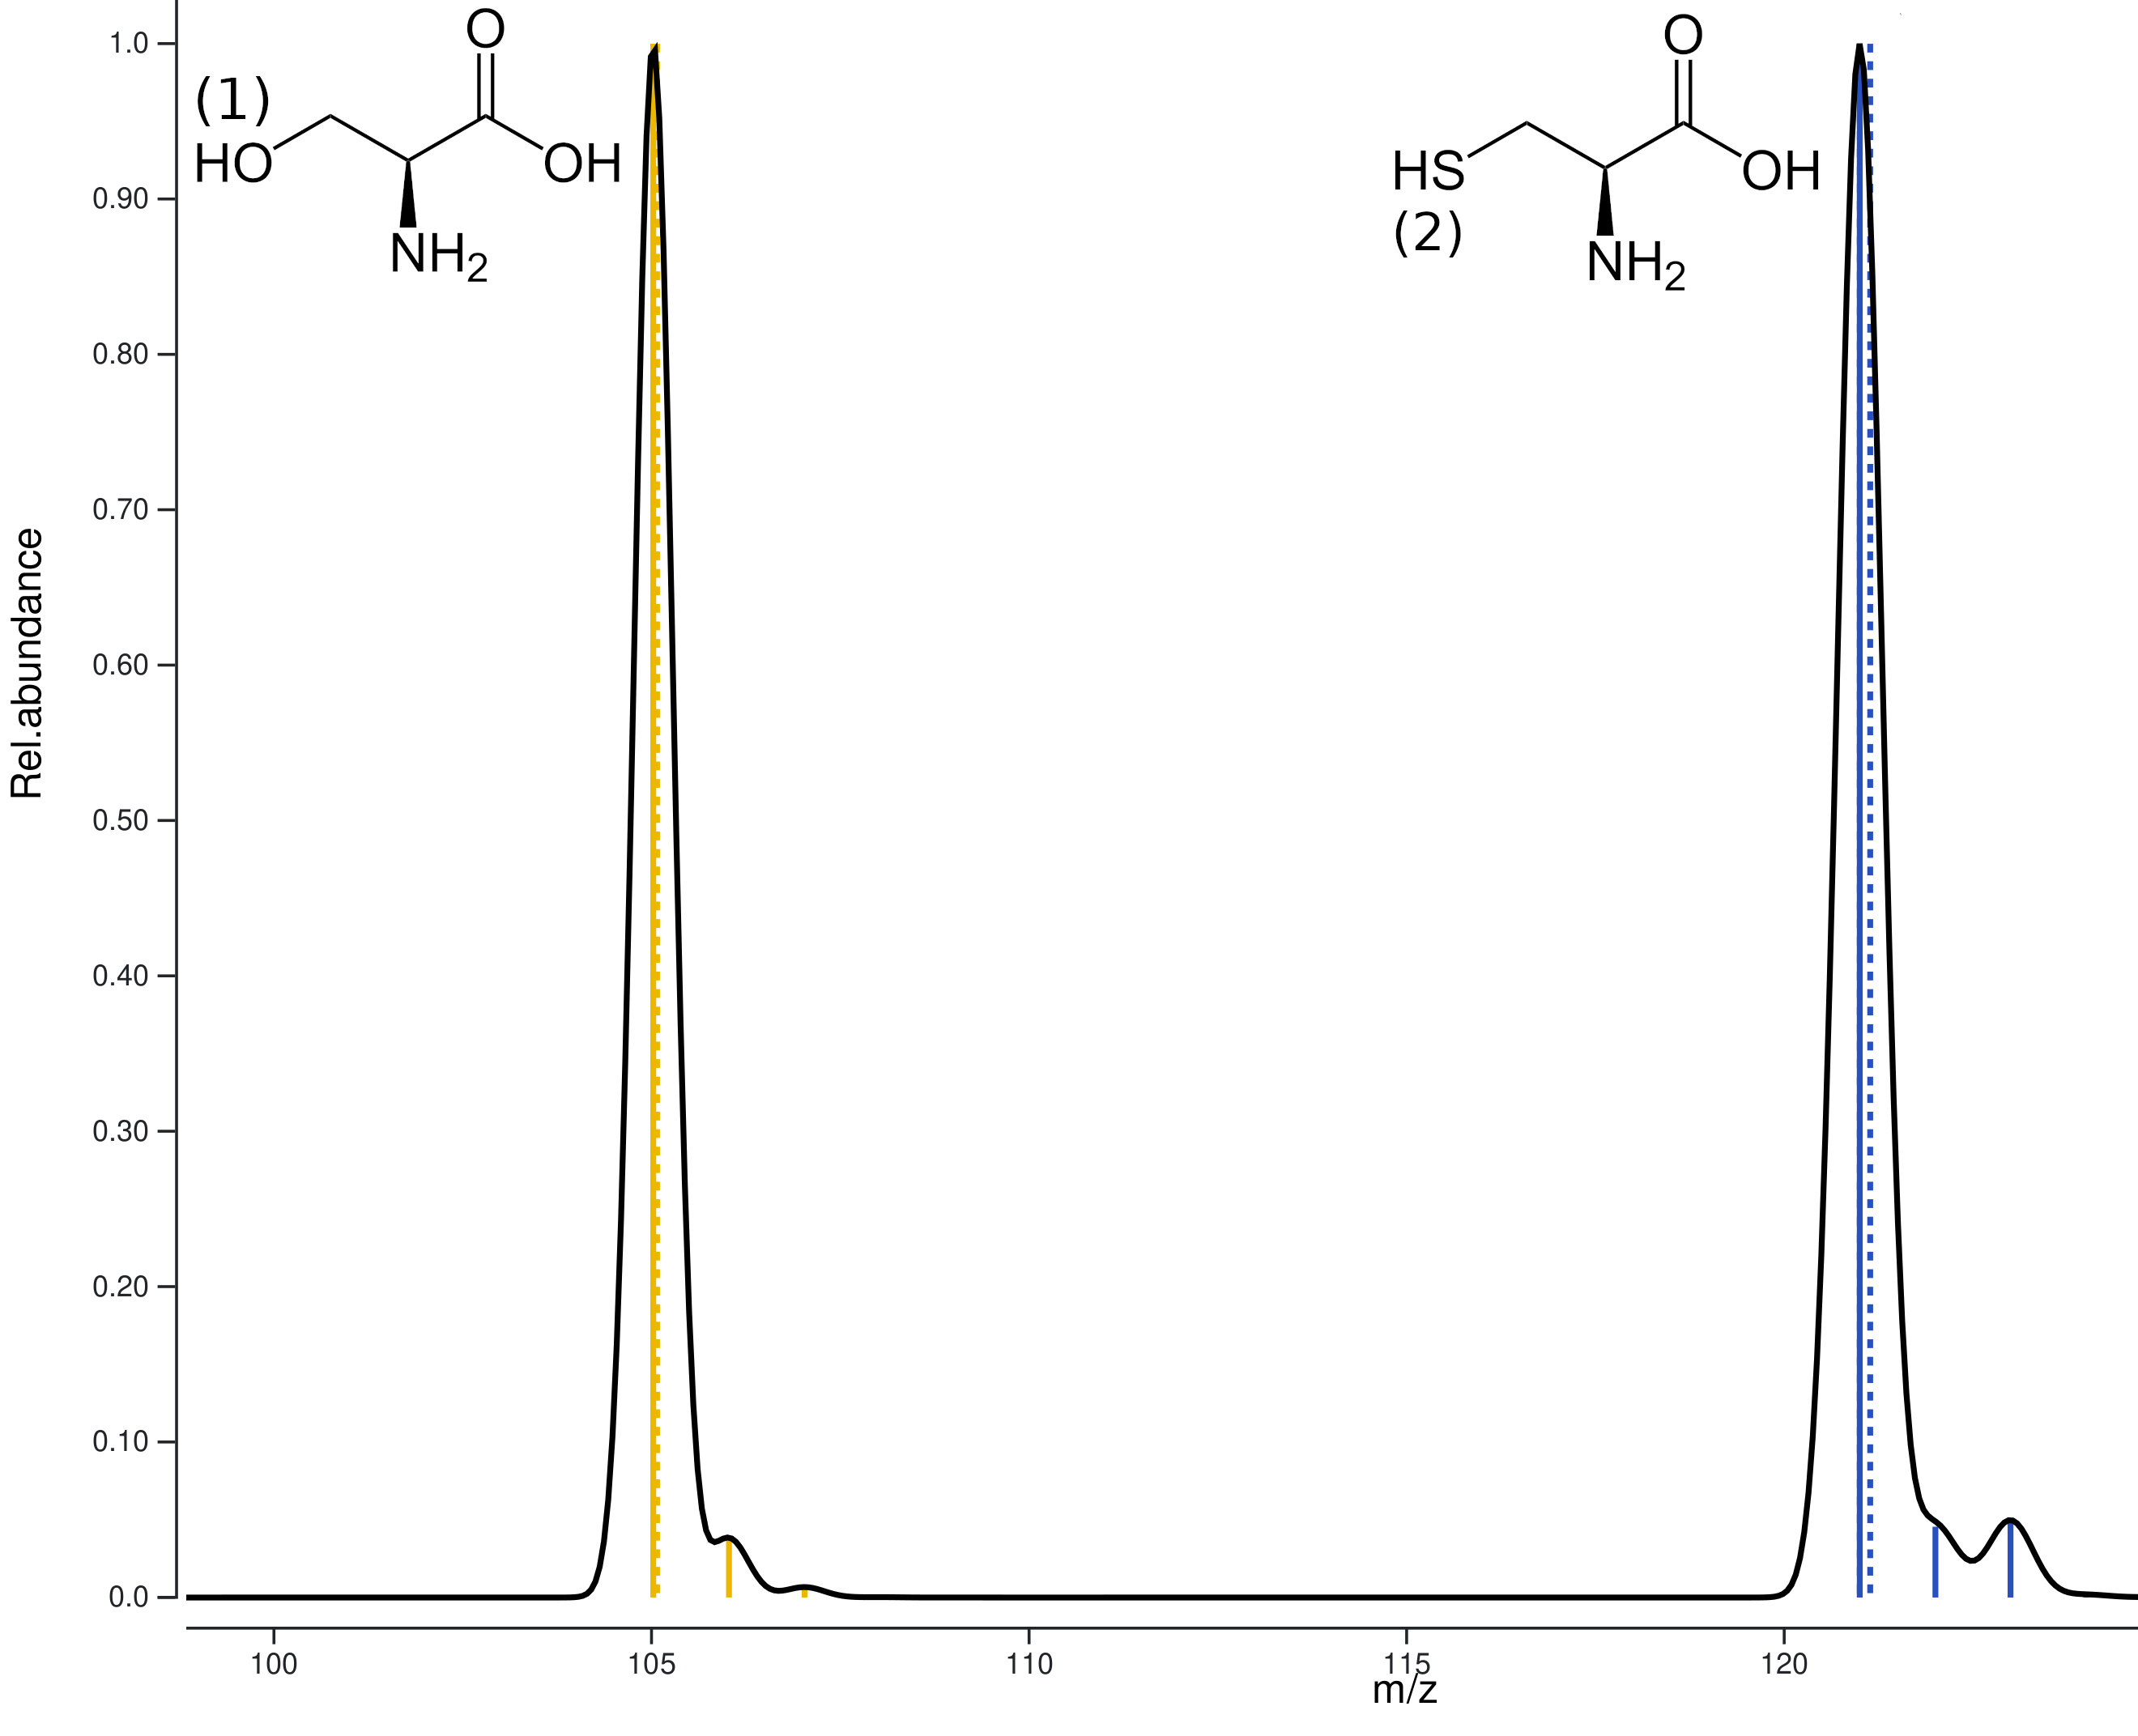
\includegraphics[width=0.75\textwidth]{./Resources/Simulated_Mass_Spectrum.png}
   \centering
   \caption{Computergeneriertes Massenspektrum von der Aminosäure \emph{Serin} (1) und \emph{Cystesin} (2). Peak von \emph{Serin} liegt bei 105; bei \emph{Systesin} um 121. y: relative Häufigkeit}
\end{figure}

Die Maxima werden \gerquot{Peaks} genannt und sind für eine Aminosäure an charakteristischer Position auf der $ x $-Achse. Obwohl sich die beiden Aminosäuren in der Abbildung \ref{fig:Sim_Mass_Spec} nur durch ein Atom unterscheiden (das linke Sauerstoffatom wurde durch ein Schwefelatom ersetzt) sind deren Massenspektren auf der $ x $-Achse weit voneinander entfernt und machen die beiden Aminosäuren dadurch sicher unterscheidbar.\\

Bei einzelnen Aminosäuren funktioniert die MS zuverlässig; bei Peptiden allerdings steht man vor dem Problem, dass das Massenspektrum unübersichtlicher wird und auch Peaks, die von Hintergrundrauschen stammen, schwerer herausgefiltert werden können. Abhilfe schafft hier die Tandem-Massenspektrometrie.

\subsection{Tandem-Massenspektrometrie (MS/MS)}\label{ss:Tandem_MS}
Bei der Tandem-Massenspektrometrie (MS/MS oder MS2) werden zwei MS Vorgänge hintereinander mit einer Probe durchgeführt. Die erste MS dient dazu Ionen aus einem bestimmten \massCharge Bereich auswählbar zu machen. Es entspricht also quasi einer Form der Filterung.

Vor der 2. MS werden die ausgewählten Reste einer Fragmentierung unterzogen. Bei einer Fragmentierung führt man Energie zu mit dem Ziel, dass die Ionen zerfallen und sog. Fragment-Ionen bilden. Diese Fragment-Ionen werden dann auf dem Massenspektrum nach der 2. MS sichtbar gemacht.

Fragment-Ionen sind kleiner als die ursprünglichen Ionen. So kann die 2. MS mit einer höheren Selektivität durchgeführt werden, welches Peaks durch Hintergrundrauschen verringert. Auch lassen sich Ionen besser identifizieren, die ein sehr ähnliches \massCharge-Verhältnis besitzen. Nach der 2. MS liegt eine Fülle an Fragment-Ionen-Peaks vor, aus denen sich die ursprünglichen Strukturinformationen ableiten lassen, da Ionen in spezifische Fragmente zerfallen \cite{Gross2013}. Zusammengefasst kann man sagen, dass das MS/MS Verfahren Ergebnisse höherer Güte erzeugt im Vergleich zur einfachen MS.

\section{De-Novo-Peptidsequenzierung mit \emph{pNovo+}}\label{s:pNovoPlusSeq}
Die \emph{pNovo+} Methode ist eine \gls{gls:DeNovo}, die mit einem \gls{gls:SpecGraph}en für die Auswertung der MS2-Spektren arbeitet und eine Erweiterung des \emph{pNovo} Verfahren darstellt \cite{pNovo}. Der Hauptansatz ist, dass zwei MS/MS Durchläufe mit jeweils verschiedenen Fragmentierungsmethoden\footnote{\emph{pNovo+} verwendet die higher energy
collisional dissociation (HCD) und die electron transfer dissociation (ETD) Fragmentierungsmethoden.} durchgeführt werden. Durch die Wahl einer anderen Fragmentierungsmethode ändert sich auch das MS2-Spektrum. Wenn nun Fragmentierungsmethoden verwendet werden, die möglichst komplementäre Spektren erzeugen, dann lässt sich durch das Zusammenführen der beiden MS2-Spektren die Qualität der Ergebnisse verbessern. Zum Beispiel lassen sich dadurch viele Peaks, die vom Hintergrundrauschen stammen, entfernen.

Für die Ermittlung der Sequenz eines Peptides wird zunächst ein Spektrums-Graph gebildet \dashAndSpace in Form eines DAG (directed acyclic graph). In diesem Graphen wird dann der längste Pfad bei gegebenen Start- und Endknoten berechnet. Die Reihenfolge der Knoten, die im längsten Pfad durchlaufen werden, stellt dann die Peptidsequenz dar.

\subsection{Vorverarbeitung der MS2-Spektren}\label{ss:Vorverarbeitung}
Bevor aus den MS2-Spektren der Spektrums-Graph gebildet werden kann, müssen die Daten vorverarbeitet werden. Für die Auswertung ist es von entscheidener Bedeutung, dass möglichst wenig Peaks verwendet werden, die vom Hintergrundrauschen stammen. Im weiteren Verlauf werden an einem exemplarischen MS2-Spektrum die Verarbeitungsschritte dargestellt.\\

Der erste Schritt ist das Verwenden des natürlichen Logarithmus der Intensitäten. Die Idee dabei ist, dass Hintergrundrauschen nicht überpriorisiert wird.

\begin{figure}[H]
   \centering
   \begin{minipage}[t]{.45\linewidth}
      \centering
      \begin{tikzpicture}[scale=\tikzScale, baseline=(current bounding box.center)]
         \draw [<->,thick] (0,\yAxisHeight) node (yaxis) [above] {\yAxisUnit}
         |- (\xAxisLength,0) node (xaxis) [right] {\xAxisUnit};
\draw[thick] (0.2, 0.0) -- (0.2, 2.3);
\draw[thick] (0.382, 0.0) -- (0.382, 1.7);
\draw[thick] (0.476, 0.0) -- (0.476, 2.7);
\draw[thick] (0.456, 0.0) -- (0.456, 1.8);
\draw[thick] (0.6859999999999999, 0.0) -- (0.6859999999999999, 2.7);
\draw[thick] (0.6839999999999999, 0.0) -- (0.6839999999999999, 1.8);
\draw[thick] (0.752, 0.0) -- (0.752, 1.1);
\draw[thick] (0.8200000000000001, 0.0) -- (0.8200000000000001, 2.2);
\draw[thick] (1.076, 0.0) -- (1.076, 1.5);
\draw[thick] (1.16, 0.0) -- (1.16, 1.9);
\draw[thick] (1.2120000000000002, 0.0) -- (1.2120000000000002, 2.0);
\draw[thick] (1.28, 0.0) -- (1.28, 1.9);
\draw[thick] (1.452, 0.0) -- (1.452, 1.3);
\draw[thick] (1.426, 0.0) -- (1.426, 1.9);
\draw[thick] (1.548, 0.0) -- (1.548, 1.9);
\draw[thick] (1.6740000000000002, 0.0) -- (1.6740000000000002, 1.5);
\draw[thick] (1.788, 0.0) -- (1.788, 2.5);
\draw[thick] (1.856, 0.0) -- (1.856, 2.3);
\draw[thick] (2.036, 0.0) -- (2.036, 1.7);
\draw[thick] (2.142, 0.0) -- (2.142, 1.6);
\draw[thick] (2.2520000000000002, 0.0) -- (2.2520000000000002, 2.0);
\draw[thick] (2.386, 0.0) -- (2.386, 1.6);
\draw[thick] (2.488, 0.0) -- (2.488, 2.9);
\draw[thick] (2.4739999999999998, 0.0) -- (2.4739999999999998, 2.7);
\draw[thick] (2.504, 0.0) -- (2.504, 2.0);
\draw[thick] (2.682, 0.0) -- (2.682, 2.0);
\draw[thick] (2.702, 0.0) -- (2.702, 2.5);
\draw[thick] (2.9259999999999997, 0.0) -- (2.9259999999999997, 2.8);
\draw[thick] (3.024, 0.0) -- (3.024, 2.4);
\draw[thick] (3.096, 0.0) -- (3.096, 1.8);
\draw[thick] (3.244, 0.0) -- (3.244, 2.6);
\draw[thick] (3.362, 0.0) -- (3.362, 1.9);
\draw[thick] (3.46, 0.0) -- (3.46, 2.3);
\draw[thick] (3.516, 0.0) -- (3.516, 1.1);
\draw[thick] (3.584, 0.0) -- (3.584, 1.8);
\draw[thick] (3.652, 0.0) -- (3.652, 2.0);
\draw[thick] (3.838, 0.0) -- (3.838, 1.5);
\draw[thick] (3.8819999999999997, 0.0) -- (3.8819999999999997, 2.6);
\draw[thick] (4.088, 0.0) -- (4.088, 2.6);
\draw[thick] (4.046, 0.0) -- (4.046, 1.1);
\draw[thick] (4.167999999999999, 0.0) -- (4.167999999999999, 2.0);
\draw[thick] (4.266, 0.0) -- (4.266, 2.4);
\draw[thick] (4.38, 0.0) -- (4.38, 1.1);
\draw[thick] (4.456, 0.0) -- (4.456, 2.2);
\draw[thick] (4.644, 0.0) -- (4.644, 2.6);
\draw[thick] (4.675999999999999, 0.0) -- (4.675999999999999, 2.5);
\draw[thick] (4.898000000000001, 0.0) -- (4.898000000000001, 1.2);
   \end{tikzpicture}%
   \end{minipage}%
   \textbf{$\rightarrow$} 
   \begin{minipage}[t]{.45\linewidth}
      \centering
      \begin{tikzpicture}[scale=\tikzScale, baseline=(current bounding box.center)]
      \draw [<->,thick] (0,\yAxisHeight) node (yaxis) [above] {\yAxisUnit}
      |- (\xAxisLength,0) node (xaxis) [right] {\xAxisUnit};
\draw[thick] (0.2, 0.0) -- (0.2, {ln(2.3)});
\draw[thick] (0.382, 0.0) -- (0.382, {ln(1.7)});
\draw[thick] (0.476, 0.0) -- (0.476, {ln(2.7)});
\draw[thick] (0.456, 0.0) -- (0.456, {ln(1.8)});
\draw[thick] (0.6859999999999999, 0.0) -- (0.6859999999999999, {ln(2.7)});
\draw[thick] (0.6839999999999999, 0.0) -- (0.6839999999999999, {ln(1.8)});
\draw[thick] (0.752, 0.0) -- (0.752, {ln(1.1)});
\draw[thick] (0.8200000000000001, 0.0) -- (0.8200000000000001, {ln(2.2)});
\draw[thick] (1.076, 0.0) -- (1.076, {ln(1.5)});
\draw[thick] (1.16, 0.0) -- (1.16, {ln(1.9)});
\draw[thick] (1.2120000000000002, 0.0) -- (1.2120000000000002, {ln(2.0)});
\draw[thick] (1.28, 0.0) -- (1.28, {ln(1.9)});
\draw[thick] (1.452, 0.0) -- (1.452, {ln(1.3)});
\draw[thick] (1.426, 0.0) -- (1.426, {ln(1.9)});
\draw[thick] (1.548, 0.0) -- (1.548, {ln(1.9)});
\draw[thick] (1.6740000000000002, 0.0) -- (1.6740000000000002, {ln(1.5)});
\draw[thick] (1.788, 0.0) -- (1.788, {ln(2.5)});
\draw[thick] (1.856, 0.0) -- (1.856, {ln(2.3)});
\draw[thick] (2.036, 0.0) -- (2.036, {ln(1.7)});
\draw[thick] (2.142, 0.0) -- (2.142, {ln(1.6)});
\draw[thick] (2.2520000000000002, 0.0) -- (2.2520000000000002, {ln(2.0)});
\draw[thick] (2.386, 0.0) -- (2.386, {ln(1.6)});
\draw[thick] (2.488, 0.0) -- (2.488, {ln(2.9)});
\draw[thick] (2.4739999999999998, 0.0) -- (2.4739999999999998, {ln(2.7)});
\draw[thick] (2.504, 0.0) -- (2.504, {ln(2.0)});
\draw[thick] (2.682, 0.0) -- (2.682, {ln(2.0)});
\draw[thick] (2.702, 0.0) -- (2.702, {ln(2.5)});
\draw[thick] (2.9259999999999997, 0.0) -- (2.9259999999999997, {ln(2.8)});
\draw[thick] (3.024, 0.0) -- (3.024, {ln(2.4)});
\draw[thick] (3.096, 0.0) -- (3.096, {ln(1.8)});
\draw[thick] (3.244, 0.0) -- (3.244, {ln(2.6)});
\draw[thick] (3.362, 0.0) -- (3.362, {ln(1.9)});
\draw[thick] (3.46, 0.0) -- (3.46, {ln(2.3)});
\draw[thick] (3.516, 0.0) -- (3.516, {ln(1.1)});
\draw[thick] (3.584, 0.0) -- (3.584, {ln(1.8)});
\draw[thick] (3.652, 0.0) -- (3.652, {ln(2.0)});
\draw[thick] (3.838, 0.0) -- (3.838, {ln(1.5)});
\draw[thick] (3.8819999999999997, 0.0) -- (3.8819999999999997, {ln(2.6)});
\draw[thick] (4.088, 0.0) -- (4.088, {ln(2.6)});
\draw[thick] (4.046, 0.0) -- (4.046, {ln(1.1)});
\draw[thick] (4.167999999999999, 0.0) -- (4.167999999999999, {ln(2.0)});
\draw[thick] (4.266, 0.0) -- (4.266, {ln(2.4)});
\draw[thick] (4.38, 0.0) -- (4.38, {ln(1.1)});
\draw[thick] (4.456, 0.0) -- (4.456, {ln(2.2)});
\draw[thick] (4.644, 0.0) -- (4.644, {ln(2.6)});
\draw[thick] (4.675999999999999, 0.0) -- (4.675999999999999, {ln(2.5)});
\draw[thick] (4.898000000000001, 0.0) -- (4.898000000000001, {ln(1.2)});
      \end{tikzpicture}
      \end{minipage}
      \caption{Anwendung des $ ln $ auf einem exemplarischen MS2-Spektrum.}
\end{figure}

Für das Verständnis des nächsten Schrittes muss man sich in Erinnerung rufen, dass eine gleiche Aminosäure keineswegs immer die gleiche Masse hat. Durch Isotope existiert eine gewisse \gerquot{Massenbandbreite} für ein und dieselbe Aminosäure. MS Systeme sind heute so genau, dass sie diese Differenzen erkennen. Dies hat den ungewollten Effekt, dass mehrere Peaks zu einer Aminosäure gehören können \cite{IsotopicDistributionMS}. Gleichzeitig können die \gerquot{Massenbandbreiten} zweier Aminosäuren sich überschneiden, sodass im ungünstigen Fall zwei Peaks kaum unterscheidbar nebeneinander liegen.\\

Eine Möglichkeit mit dieser Problematik umzugehen ist die Verwendung der monoisotopischen Masse. Die monoisotopische Masse ist die \gerquot{[...] exact mass of the most abundant naturally occurring stable isotope determined relative to the mass of 12 C, which is assigned the exact value of 12.0000.} \cite{MonoisotopicMass}. Ohne dabei jetzt tiefer ins Detail zu gehen kann man sagen, dass alle Peaks, deren Intensität mit einer möglichen monoisotopischen Masse übereinstimmen, auf jeden Fall einer Aminosäure entsprechen und (höchstwahrscheinlich)\footnote{Natürlich ist es möglich, dass das Rauschen zufällig einer monoisotopischen Masse entspricht. Die Wahrscheinlichkeit dafür ist allerdings sehr gering.} kein Hintergrundrauschen sind \cite{MassDefectMS}. Diese Peaks bekommen eine sogennante \emph{charge state}.\\

Der Algorithmus verwendet die \emph{charge state} Peaks als Ausganspunkte für weitere Berechnungen. Wenn die \massCharge Differenz zu einem anderen Peak einem Peptidfragment entspricht, dann stammt dieser Peak höchstwahrscheinlich von einem Fragment. Insgesamt werden damit die relevanten Peptidfragmente herausgeholt. Abbildung \ref{MonoisotopicMassFiltering} zeigt das Ergebnis nach den beiden zuvor genannten Schritten.

\begin{figure}[H]\label{MonoisotopicMassFiltering}
   \centering
   \begin{minipage}[t]{.45\linewidth}
      \centering
      \begin{tikzpicture}[scale=\tikzScale, baseline=(current bounding box.center)]
         \draw [<->,thick] (0,\yAxisHeight) node (yaxis) [above] {\yAxisUnit}
         |- (\xAxisLength,0) node (xaxis) [right] {\xAxisUnit};
\draw[thick] (0.2, 0.0) -- (0.2, {ln(2.3)});
\draw[color=blue!85!,opacity=.55,thick] (0.382, 0.0) -- (0.382, {ln(1.7)});
\draw[color=blue!85!,opacity=.55,thick] (0.476, 0.0) -- (0.476, {ln(2.7)});
\draw[color=magenta,thick] (0.456, 0.0) -- (0.456, {ln(1.8)});
\draw[color=blue!85!,opacity=.55,thick] (0.6859999999999999, 0.0) -- (0.6859999999999999, {ln(2.7)});
\draw[color=blue!85!,opacity=.55,thick] (0.6839999999999999, 0.0) -- (0.6839999999999999, {ln(1.8)});
\draw[thick] (0.752, 0.0) -- (0.752, {ln(1.1)});
\draw[thick] (0.8200000000000001, 0.0) -- (0.8200000000000001, {ln(2.2)});
\draw[thick] (1.076, 0.0) -- (1.076, {ln(1.5)});
\draw[thick] (1.16, 0.0) -- (1.16, {ln(1.9)});
\draw[thick] (1.2120000000000002, 0.0) -- (1.2120000000000002, {ln(2.0)});
\draw[thick] (1.28, 0.0) -- (1.28, {ln(1.9)});
\draw[color=blue!85!,opacity=.55,thick] (1.452, 0.0) -- (1.452, {ln(1.3)});
\draw[color=blue!85!,opacity=.55,thick] (1.426, 0.0) -- (1.426, {ln(1.9)});
\draw[color=magenta,thick] (1.548, 0.0) -- (1.548, {ln(1.9)});
\draw[color=blue!85!,opacity=.55,thick] (1.6740000000000002, 0.0) -- (1.6740000000000002, {ln(1.5)});
\draw[color=blue!85!,opacity=.55,thick] (1.788, 0.0) -- (1.788, {ln(2.5)});
\draw[thick] (1.856, 0.0) -- (1.856, {ln(2.3)});
\draw[thick] (2.036, 0.0) -- (2.036, {ln(1.7)});
\draw[thick] (2.142, 0.0) -- (2.142, {ln(1.6)});
\draw[thick] (2.2520000000000002, 0.0) -- (2.2520000000000002, {ln(2.0)});
\draw[thick] (2.386, 0.0) -- (2.386, {ln(1.6)});
\draw[color=blue!85!,opacity=.55,thick] (2.488, 0.0) -- (2.488, {ln(2.9)});
\draw[thick] (2.4739999999999998, 0.0) -- (2.4739999999999998, {ln(2.7)});
\draw[color=blue!85!,opacity=.55,thick] (2.504, 0.0) -- (2.504, {ln(2.0)});
\draw[color=magenta,thick] (2.682, 0.0) -- (2.682, {ln(2.0)});
\draw[color=blue!85!,opacity=.55,thick] (2.702, 0.0) -- (2.702, {ln(2.5)});
\draw[thick] (2.9259999999999997, 0.0) -- (2.9259999999999997, {ln(2.8)});
\draw[thick] (3.024, 0.0) -- (3.024, {ln(2.4)});
\draw[thick] (3.096, 0.0) -- (3.096, {ln(1.8)});
\draw[thick] (3.244, 0.0) -- (3.244, {ln(2.6)});
\draw[thick] (3.362, 0.0) -- (3.362, {ln(1.9)});
\draw[color=blue!85!,opacity=.55,thick] (3.46, 0.0) -- (3.46, {ln(2.3)});
\draw[color=blue!85!,opacity=.55,thick] (3.516, 0.0) -- (3.516, {ln(1.1)});
\draw[color=blue!85!,opacity=.55,thick] (3.584, 0.0) -- (3.584, {ln(1.8)});
\draw[color=magenta,thick] (3.652, 0.0) -- (3.652, {ln(2.0)});
\draw[color=blue!85!,opacity=.55,thick] (3.838, 0.0) -- (3.838, {ln(1.5)});
\draw[color=blue!85!,opacity=.55,thick] (3.8819999999999997, 0.0) -- (3.8819999999999997, {ln(2.6)});
\draw[thick] (4.088, 0.0) -- (4.088, {ln(2.6)});
\draw[thick] (4.046, 0.0) -- (4.046, {ln(1.1)});
\draw[thick] (4.167999999999999, 0.0) -- (4.167999999999999, {ln(2.0)});
\draw[thick] (4.266, 0.0) -- (4.266, {ln(2.4)});
\draw[color=blue!85!,opacity=.55,thick] (4.38, 0.0) -- (4.38, {ln(1.1)});
\draw[color=blue!85!,opacity=.55,thick] (4.456, 0.0) -- (4.456, {ln(2.2)});
\draw[color=magenta,thick] (4.644, 0.0) -- (4.644, {ln(2.6)});
\draw[color=blue!85!,opacity=.55,thick] (4.675999999999999, 0.0) -- (4.675999999999999, {ln(2.5)});
\draw[color=blue!85!,opacity=.55,thick] (4.898000000000001, 0.0) -- (4.898000000000001, {ln(1.2)});
   \end{tikzpicture}%
   \end{minipage}%
   \textbf{$\rightarrow$} 
   \begin{minipage}[t]{.45\linewidth}
      \centering
      \begin{tikzpicture}[scale=\tikzScale, baseline=(current bounding box.center)]
      \draw [<->,thick] (0,\yAxisHeight) node (yaxis) [above] {\yAxisUnit}
      |- (\xAxisLength,0) node (xaxis) [right] {\xAxisUnit};
\draw[color=blue!85!,opacity=.55,thick] (0.382, 0.0) -- (0.382, {ln(1.7)});
\draw[color=blue!85!,opacity=.55,thick] (0.476, 0.0) -- (0.476, {ln(2.7)});
\draw[color=magenta,thick] (0.456, 0.0) -- (0.456, {ln(1.8)});
\draw[color=blue!85!,opacity=.55,thick] (0.6859999999999999, 0.0) -- (0.6859999999999999, {ln(2.7)});
\draw[color=blue!85!,opacity=.55,thick] (0.6839999999999999, 0.0) -- (0.6839999999999999, {ln(1.8)});
\draw[color=blue!85!,opacity=.55,thick] (1.452, 0.0) -- (1.452, {ln(1.3)});
\draw[color=blue!85!,opacity=.55,thick] (1.426, 0.0) -- (1.426, {ln(1.9)});
\draw[color=magenta,thick] (1.548, 0.0) -- (1.548, {ln(1.9)});
\draw[color=blue!85!,opacity=.55,thick] (1.6740000000000002, 0.0) -- (1.6740000000000002, {ln(1.5)});
\draw[color=blue!85!,opacity=.55,thick] (1.788, 0.0) -- (1.788, {ln(2.5)});
\draw[color=blue!85!,opacity=.55,thick] (2.488, 0.0) -- (2.488, {ln(2.9)});
\draw[color=blue!85!,opacity=.55,thick] (2.504, 0.0) -- (2.504, {ln(2.0)});
\draw[color=magenta,thick] (2.682, 0.0) -- (2.682, {ln(2.0)});
\draw[color=blue!85!,opacity=.55,thick] (2.702, 0.0) -- (2.702, {ln(2.5)});
\draw[color=blue!85!,opacity=.55,thick] (3.46, 0.0) -- (3.46, {ln(2.3)});
\draw[color=blue!85!,opacity=.55,thick] (3.516, 0.0) -- (3.516, {ln(1.1)});
\draw[color=blue!85!,opacity=.55,thick] (3.584, 0.0) -- (3.584, {ln(1.8)});
\draw[color=magenta,thick] (3.652, 0.0) -- (3.652, {ln(2.0)});
\draw[color=blue!85!,opacity=.55,thick] (3.838, 0.0) -- (3.838, {ln(1.5)});
\draw[color=blue!85!,opacity=.55,thick] (3.8819999999999997, 0.0) -- (3.8819999999999997, {ln(2.6)});
\draw[color=blue!85!,opacity=.55,thick] (4.38, 0.0) -- (4.38, {ln(1.1)});
\draw[color=blue!85!,opacity=.55,thick] (4.456, 0.0) -- (4.456, {ln(2.2)});
\draw[color=magenta,thick] (4.644, 0.0) -- (4.644, {ln(2.6)});
\draw[color=blue!85!,opacity=.55,thick] (4.675999999999999, 0.0) -- (4.675999999999999, {ln(2.5)});
\draw[color=blue!85!,opacity=.55,thick] (4.898000000000001, 0.0) -- (4.898000000000001, {ln(1.2)});
      \end{tikzpicture}
      \end{minipage}
      \caption{Entfernen von Peaks, die keiner monoisotopischen Masse entsprechen oder benachbart mit einer Differenz von einem Fragment-Ion sind.}
\end{figure}

Tatsächlich ist die Verarbeitung an dieser Stelle noch etwas komplexer. So existieren auch noch sogenannte \emph{isotopic cluster}\footnote{Definition eines \emph{isotopic cluster} nach IUPAC: \gerquot{Group of peaks representing ions of the same elemental composition, but different isotopic compositions.} \cite[1556]{IUPACDefinitions}}, die gesondert verarbeitet werden. Für das grundsätzliche Prinzip ist dieses Detail allerdings weniger relevant.\\

Im letzten Vorberarbeitungsschritt werden Peaks aus einem irrelevanten \massCharge Bereich entfernt und naheliegende Peaks werden zusammengefasst, indem der Mittelwert sowol des \massCharge Wertes als auch der der Intensität besimmt wird. Üblicherweise liegt der Bereich für das Zusammenfassen bei $ +- 20 ppm $.

\begin{figure}[H]
   \centering
   \begin{minipage}[t]{.45\linewidth}
      \centering
      \begin{tikzpicture}[scale=\tikzScale, baseline=(current bounding box.center)]
         \draw [<->,thick] (0,\yAxisHeight) node (yaxis) [above] {\yAxisUnit}
         |- (\xAxisLength,0) node (xaxis) [right] {\xAxisUnit};
\draw[thick] (0.382, 0.0) -- (0.382, {ln(1.7)});
\draw[thick] (0.476, 0.0) -- (0.476, {ln(2.7)});
\draw[thick] (0.456, 0.0) -- (0.456, {ln(1.8)});
\draw[thick] (0.6859999999999999, 0.0) -- (0.6859999999999999, {ln(2.7)});
\draw[thick] (0.6839999999999999, 0.0) -- (0.6839999999999999, {ln(1.8)});
\draw[color=red,thick] (1.452, 0.0) -- (1.452, {ln(1.3)});
\draw[color=red,thick] (1.426, 0.0) -- (1.426, {ln(1.9)});
\draw[thick] (1.548, 0.0) -- (1.548, {ln(1.9)});
\draw[thick] (1.6740000000000002, 0.0) -- (1.6740000000000002, {ln(1.5)});
\draw[thick] (1.788, 0.0) -- (1.788, {ln(2.5)});
\draw[color=red,thick] (2.488, 0.0) -- (2.488, {ln(2.9)});
\draw[color=red,thick] (2.504, 0.0) -- (2.504, {ln(2.0)});
\draw[color=red,thick] (2.682, 0.0) -- (2.682, {ln(2.0)});
\draw[color=red,thick] (2.702, 0.0) -- (2.702, {ln(2.5)});
\draw[thick] (3.46, 0.0) -- (3.46, {ln(2.3)});
\draw[thick] (3.516, 0.0) -- (3.516, {ln(1.1)});
\draw[thick] (3.584, 0.0) -- (3.584, {ln(1.8)});
\draw[thick] (3.652, 0.0) -- (3.652, {ln(2.0)});
\draw[color=red,thick] (3.838, 0.0) -- (3.838, {ln(1.5)});
\draw[color=red,thick] (3.8819999999999997, 0.0) -- (3.8819999999999997, {ln(2.6)});
\draw[thick] (4.38, 0.0) -- (4.38, {ln(1.1)});
\draw[thick] (4.456, 0.0) -- (4.456, {ln(2.2)});
\draw[thick] (4.644, 0.0) -- (4.644, {ln(2.6)});
\draw[thick] (4.675999999999999, 0.0) -- (4.675999999999999, {ln(2.5)});
\draw[thick] (4.898000000000001, 0.0) -- (4.898000000000001, {ln(1.2)});

\fill[red!25!,opacity=.25] (0,0) rectangle (1,\yAxisHeight-\axisColorOffset);
         \fill[red!25!,opacity=.25] (\xAxisLength-1,0) rectangle (\xAxisLength-\axisColorOffset,\yAxisHeight-\axisColorOffset);
         \fill[green!25!,opacity=.25] (1,0) rectangle (\xAxisLength-1,\yAxisHeight-\axisColorOffset);
   \end{tikzpicture}%
   \end{minipage}%
   \textbf{$\rightarrow$} 
   \begin{minipage}[t]{.45\linewidth}
      \centering
      \begin{tikzpicture}[scale=\tikzScale, baseline=(current bounding box.center)]
      \draw [<->,thick] (0,\yAxisHeight) node (yaxis) [above] {\yAxisUnit}
      |- (\xAxisLength,0) node (xaxis) [right] {\xAxisUnit};
%\draw[color=red,thick] (1.452, 0.0) -- (1.452, {ln(1.3)});
%\draw[color=red,thick] (1.426, 0.0) -- (1.426, {ln(1.9)});
\draw[color=red,ultra thick] ({(1.452+1.426)/2}, 0.0) -- ({(1.452+1.426)/2}, {(ln(1.3)+ln(1.9))/2});

\draw[thick] (1.548, 0.0) -- (1.548, {ln(1.9)});
\draw[thick] (1.6740000000000002, 0.0) -- (1.6740000000000002, {ln(1.5)});
\draw[thick] (1.788, 0.0) -- (1.788, {ln(2.5)});

%\draw[color=red,thick] (2.488, 0.0) -- (2.488, {ln(2.9)});
%\draw[color=red,thick] (2.504, 0.0) -- (2.504, {ln(2.0)});
\draw[color=red,ultra thick] ({(2.488+2.504)/2}, 0.0) -- ({(2.488+2.504)/2}, {(ln(2.9)+ln(2.0))/2});

%\draw[color=red,thick] (2.682, 0.0) -- (2.682, {ln(2.0)});
%\draw[color=red,thick] (2.702, 0.0) -- (2.702, {ln(2.5)});
\draw[color=red,ultra thick] ({(2.682+2.702)/2}, 0.0) -- ({(2.682+2.702)/2}, {(ln(2.0+ln(2.5))/2});

\draw[thick] (3.46, 0.0) -- (3.46, {ln(2.3)});
\draw[thick] (3.516, 0.0) -- (3.516, {ln(1.1)});
\draw[thick] (3.584, 0.0) -- (3.584, {ln(1.8)});
\draw[thick] (3.652, 0.0) -- (3.652, {ln(2.0)});

%\draw[color=red,thick] (3.838, 0.0) -- (3.838, {ln(1.5)});
%\draw[color=red,thick] (3.8819999999999997, 0.0) -- (3.8819999999999997,{ln(2.6)});
\draw[color=red,ultra thick] ({(3.838+3.8819999999999997)/2}, 0.0) -- ({(3.838+3.8819999999999997)/2}, {(ln(1.5)+ln(2.6))/2});

\fill[red!25!,opacity=.25] (0,0) rectangle (1,\yAxisHeight-\axisColorOffset);
         \fill[red!25!,opacity=.25] (\xAxisLength-1,0) rectangle (\xAxisLength-\axisColorOffset,\yAxisHeight-\axisColorOffset);
         \fill[green!25!,opacity=.25] (1,0) rectangle (\xAxisLength-1,\yAxisHeight-\axisColorOffset);
      \end{tikzpicture}
      \end{minipage}
      \caption{Entfernen von Peaks aus einem irrelevanten \massCharge Bereich und zusammenfassen naheliegender Peaks. Rot markierte Peaks sind jene, die zusammengefasst werden.}
\end{figure}

\subsection{Bildung eines Spektrums-Graphen}\label{ss:BildungSpekGraph}
Der Spektrums-Graph wird aus einem vorverarbeiteten MS2-Spektrum (siehe Kapitel: \ref{ss:Vorverarbeitung}) gebildet. Im initialen Zustand werden die Peaks als Knoten interpretiert. Dazu kommt ein Start- und Endknoten. Jedem Knoten wird eine Masse zugeordet; im initialen Zustand bekommt der Startknoten die Masse 0 und der Endknoten die Masse des vorherigen Knotens minus der Masse des Wassers ($ 18,02 $). Die Masse der übrigen Knoten entsprechen ihren jeweils korrespondierenden \massCharge Wert. Die gerichteten Kanten werden zwischen einem Knotenpaar hinzugefügt, wenn die Differenz deren Masse gleich ist mit der Masse von ein oder zwei Aminosäuren.

\subsection{Identifikation der Aminosäuresequenz}
Der gebildete DAG kann mit klassischen Algorithmen, die den längsten Pfad suchen, durchlaufen werden. Bezogen auf die Graphentheorie entspricht die Ermittlung der Aminosäurensequenz dem Suchen eines bestimmten Pfades \dashAndSpace und nicht nach irgendeinem Pfad. Daher muss der Algorithmus mittels einer Breitensuche arbeiten, um alle möglichen Pfade zu bestimmen.

In aller Regel wird es mehrere Pfade geben. Bestimmte Sequenzen sind wahrscheinlicher als andere. So sind Pfade mit Kanten, die wegen der Massendifferenz von genau einer Aminosäure gebildet wurden, wahrscheinlicher \cite{pNovoPlus}. Alle Pfade bekommen mittels einer Scoring-Funktion einen Wert zugewiesen. Der Pfad mit dem höchsten Scoring-Wert ist wahrscheinlich das richtige Ergebnis. Die Scoring-Funktion berücksichtigt unter anderem wie viele Fragmente, die einer bestimmten Aminosäure zugeordet werden können, im MS2-Spektrum vorhanden sind \cite{pNovo}. Die Sequenz mit dem höchsten Scoring-Wert ist das Endergebnis.

\section{De-Novo-Peptidsequenzierung mit \emph{Open-pNovo}}\label{s:OpenpNovoSeq}
Bei Proteinen können posttranslationale Proteinmodifikationen (PTM) auftreten. PTMs sind Ereignisse, bei denen sich Änderungen im Protein einstellen \cite{Mann2003}; teilweise sind die Änderungen von einer Zelle erwünscht \dashAndSpace teilweise stammen sie aber auch zum Beispiel von unerwünschten Wechselwirkungen nebeneinanderliegenden Aminosäuren. Ein Teil dieser PTMs führen zu einer Änderung der Aminosäuresequenz. Dies ist für die \gls{gls:DeNovo} nicht weiter problematisch, da sowieso ohne eine Datenbank gearbeitet wird, sodass solche PTMs nicht einmal auffallen würden. Andere PTMs hingegen haben die Auswirkung, dass Stoffe gebildet werden, die nicht mehr zu der Gruppe der proteinogenen Aminosäuren gehören. Proteinogene Aminosäuren sind jene Aminosäuren, die für den Bau von Proteinen verwendet werden. Der Effekt ist also, dass Stoffe (oder deren Fragmente) bei einem Massenspektrum angezeigt werden, die kein Teil eines Peptids sein können. Bei der Sequenzierung von Peptidfragmenten muss dies daher berücksichtigt werden.
Wenn im weiteren Verlauf von PTMs gesprochen wird, dann sind solche gemeint, die für die \gls{gls:DeNovo} relevant sind.

Open-pNovo ist ein \gls{gls:DeNovo}sverfahren, welches auf pNovo+ Tool aufbaut und versucht die Problematik mit den PTMs zu lösen.

\subsection{PTMs im konstruierten DAG}
Die Konvertierung eines MS2-Spektrums läuft bis zum DAG analog ab wie in den Kapiteln \ref{ss:Vorverarbeitung} und \ref{ss:BildungSpekGraph} für pNovo+. Der Unterschied ist nun, dass es zwei Arten von Kanten gibt:

\begin{itemize}
   \item \gerquot{Normale} Kanten: Kanten, die gebildet werden, wie es bereits für \emph{pNovo+} gezeigt wurde. 
   \item \gerquot{Modifizierte} Kanten: Kanten, die zum Grahpen hinzugefügt werden, wenn die Massendifferenz zweier Knoten der Masse einer Aminosäure plus der Masse einer möglichen PTM-Änderung entspricht. 
\end{itemize}

Eine Liste aller PTMs in der Datenbank Unimod (sowohl relevante als auch nicht relevante) beinhaltet aktuell 1510 Einträge\footnote{Siehe: \url{https://www.ebi.ac.uk/ols/ontologies/unimod}} (Stand: 18.04.2022). Für die modifizierten Kanten gibt es insgesamt $ 1510 * 20 = 30200 $ mögliche Differenzen, wobei viele davon nicht relevante PTMs sind. Zum Vergleich: bei den normalen Kanten gibt es $ 20^2 = 400 $ mögliche Differenzen.

Die hohe Anzahl an Differenzen für modifizierte Kanten hat die Konsequenz, dass viele Knoten zufällig verbunden werden und dass dadurch die Genauigkeit der Ergebnisse abnimmt. Dieses Problem kann man durch eine geringere Liste an möglichen PTMs abfedern, allerdings mit einem Verlust  der Genauigkeit auf Seiten der PTMs. Es ist hier also eine Abwägung.

\subsection{Evaluierung von Open-pNovo}
Open-pNovo wurde sowohl auf drei realen als auch auf drei generierten Testdaten getestet. Tabelle \ref{tab:OpenPNovoResults} zeigt die Ergebnisse im Vergleich zu pNovo+ und zwei anderen Algorithmen. Die Datensätze enthielten die am häufigsten vorkommenden PTMs.

\begin{table}[H]
    \centering
    \begin{tabular}{l|c|c|c|c}
        \toprule
        \textbf{Testdatensätze} & \textbf{Open-pNovo+} & \textbf{pNovo+} & \textbf{PEAKS} & \textbf{Novor} \\
        \midrule
        Real (20259) & $76,3 \%$ & $68,5 \%$ & $65,8 \%$ & $39,9 \%$ \\
        Generiert (17877) & $77,8 \%$ & $0,6 \%$ & $0,5 \%$ & $0,2 \%$ \\
        \bottomrule
    \end{tabular}
    \newline
    \caption{Vergleich der durchschnittlichen richtigen \gls{gls:DeNovo} Peptidsequenzierungen von Open-pNovo und anderen Algorithmen \cite[650]{OpenPNovo}.}
    \label{tab:OpenPNovoResults}
\end{table}

Die enorm schlechten Ergebnisse der anderen Algorithmen bei den generierten Testdaten ist ein Nebeneffekt des Ziels bei der Testdatengenerierung. Denn diese wurden so ausgelegt, um die Grenzen von Open-pNovo+ zu ermitteln \cite[649]{OpenPNovo}. Eine Aussagekraft haben diese Ergebnisse also nicht. Allerdings auch bei realen Testdaten zeigt sich Open-pNovo als voll konkurrenzfähig gegenüber den anderen Algorithmen.

Noch besser zeigt sich Open-pNovo, wenn der Recall Wert betrachtet wird \dashAndSpace also die Anzahl an verschiedenen PSMs, die erkannt wurden. In diesem Fall ist der Abstand zu den anderen Algorithmen deutlich größer geworden.

\begin{table}[H]
    \centering
    \begin{tabular}{l|c|c|c|c}
        \toprule
        \textbf{Testdatensätze} & \textbf{Open-pNovo+} & \textbf{pNovo+} & \textbf{PEAKS} & \textbf{Novor} \\
        \midrule
        Real (5034) & $61,6 \%$ & $31,3 \%$ & $32,0 \%$ & $13,7 \%$ \\
        \bottomrule
    \end{tabular}
    \newline
    \caption{Vergleich der durchschnittlichen Recall Werte einer \gls{gls:DeNovo} Peptidsequenzierungen von Open-pNovo und anderen Algorithmen \cite[650]{OpenPNovo}.}
    \label{tab:OpenPNovoResultsRecall}
\end{table}

\subsection{Zusammenfassung}


% Die \gls{gls:DeNovo} nutzt die sogenannte \gls{gls:TMassSpek} für die Bestimmung der Peptidsequenz. Dabei wird die physikalische Eigenschaft ausgenutzt, dass jedes Atom bzw. jedes Molekül \dashAndSpace wenn es einer \gls{gls:Ionisation} unterzogen wurde \dashAndSpace ein charakteristisches \gls{gls:MassSpek} besitzt. Das \gls{gls:MassSpek} stellt also eine Art \gerquot{Fingerabdruck} eines Moleküls dar und macht dieses ermittelbar.

% U.U. eine Beispielgrafik eines Massenspektrums hinzufuegen ...

\subsubsection{\glsentrytext{gls:TMassSpek} bei größeren Molekülen}
Bei größeren Molekülen (wie einem Protein) führt die \gls{gls:Ionisation} dazu, dass das Molekül in kleinere spezifische Ionen zerfällt (sog. Fragmentierung). Die Fragmentierungsinformationen einer \gls{gls:DeNovo} sind meist unvollständig, da fehlende Daten bei einem Fragmentierungsschritt die Güte des Endergebnisses negativ beeinflusst. Dies wird insbesondere dann ein Problem, wenn unbekannte Änderungen in einer Peptidsequenz vorhanden sind.

Um dieses Problem zu verringern können unterschiedliche Techniken parallel eingesetzt werden, welche verschiedene Fragmente erzeugen und daher auch verschiedenartige \glspl{gls:MassSpek} zur Folge haben.\footnote{Konkret: Es wird sowohl das \gls{acr:HCD} als auch das \gls{acr:ETD} Verfahren angewendet.}

\subsection{Datenaufbereitung}
Typischerweise betrachtet man die sog. \gerquot{\glspl{gls:Peak}} in den \glspl{gls:MassSpek}. Jeder \gls{gls:Peak} stellt ein unterschiedliches Ion dar. Dazu kommen Messungenauigkeiten sowie Hintergrundrauschen. Durch die hohe Anzahl an möglichen Ionen kann nicht ohne weiteres differenziert werden, welcher der \glspl{gls:Peak} von welchen Ionen erzeugt wurden und welche nicht.

% Frage an Dominik: Ist hier eine einfache Auflistung an Techniken für die Datenaufbereitung besser?
Der Algorithmus für die Datenaufbereitung berechnet den natürlichen Logarithmus von den Intensitäten der \glspl{gls:Peak}, um Hintergrundrauschen und Messungenauigkeiten nicht überzupriorisieren. Zusätzlich dazu werden \glspl{gls:Peak}, die in einem Toleranzbereich nebeneinander liegen, zusammengefasst. Am Ende werden die \glspl{gls:Peak} entfernt, bei denen bekannt ist, dass es sich nicht um relevante Ionen handeln kann. (z.B. \glspl{gls:Peak} von Isotopen)

\begin{figure}[H]
   \centering
   \begin{minipage}[t]{.4\linewidth}
      \centering
      \begin{tikzpicture}[scale=\tikzScale, baseline=(current bounding box.center)]
         \draw [<->,thick] (0,2.75) node (yaxis) [above] {\yAxisUnit}
         |- (3,0) node (xaxis) [right] {\xAxisUnit};

         \draw[thick] (0.2,0) -- (0.2,1.1);
         \draw[thick] (0.3,0) -- (0.3,1.6);
         \draw[thick] (0.6,0) -- (0.6,1.7);
         \draw[thick] (0.8,0) -- (0.8,1.2);
         \draw[thick] (1.0,0) -- (1.0,1.1);

         \draw[color=red,thick] (1.2,0) -- (1.2,2.65);
         \draw[thick] (1.4,0) -- (1.4,1.4);
         \draw[thick] (1.6,0) -- (1.6,1.2);
         \draw[thick] (1.8,0) -- (1.8,1.3);
         \draw[thick] (2.0,0) -- (2.0,1.8);

         \draw[thick] (1.1,0) -- (1.1,2.0);
         \draw[color=red,thick] (0.35,0) -- (0.35,2.25);
         \draw[thick] (1.9,0) -- (1.9,1.4);
         \draw[color=red,thick] (2.2,0) -- (2.2,2.6);
         \draw[thick] (2.5,0) -- (2.5,1.25);

         \draw[thick] (2.7,0) -- (2.7,1.1);
         \foreach \x in {1,...,6}
         {
            \draw[thick] (1.2+\x*0.05,0) -- (1.2+\x*0.05,1.0+\x*0.15);
         }
      \end{tikzpicture}%
      % \subcaption{Exemplarische Rohdaten}
   \end{minipage}%
   \textbf{$\rightarrow$}
   \begin{minipage}[t]{.4\linewidth}
      \centering
      \begin{tikzpicture}[scale=\tikzScale, baseline=(current bounding box.center)]
         \draw [<->,thick] (0,2.75) node (yaxis) [above] {\yAxisUnit}
         |- (3,0) node (xaxis) [right] {\xAxisUnit};

         \draw[thick] (0.2,0) -- (0.2,{ln(1.1)});
         \draw[thick] (0.3,0) -- (0.3,{ln(1.6)});
         \draw[thick] (0.6,0) -- (0.6,{ln(1.7)});
         \draw[thick] (0.8,0) -- (0.8,{ln(1.2)});
         \draw[thick] (1.0,0) -- (1.0,{ln(1.1)});

         \draw[color=red,thick] (1.2,0) -- (1.2,{ln(2.65)});
         \draw[thick] (1.4,0) -- (1.4,{ln(1.4)});
         \draw[thick] (1.6,0) -- (1.6,{ln(1.2)});
         \draw[thick] (1.8,0) -- (1.8,{ln(1.3)});
         \draw[thick] (2.0,0) -- (2.0,{ln(1.8)});

         \draw[thick] (1.1,0) -- (1.1,{ln(2.0)});
         \draw[color=red,thick] (0.35,0) -- (0.35,{ln(2.25)});
         \draw[thick] (1.9,0) -- (1.9,{ln(1.4)});
         \draw[color=red,thick] (2.2,0) -- (2.2,{ln(2.6)});
         \draw[thick] (2.5,0) -- (2.5,{ln(1.25)});

         \draw[thick] (2.7,0) -- (2.7,{ln(1.1)});
         \foreach \x in {1,...,6}
         {%
            \draw[thick] (1.2+\x*0.05,0) -- (1.2+\x*0.05,{ln(1.0+\x*0.15)});
         }
      \end{tikzpicture}
      %\subcaption{Exemplarische Rohdaten}
   \end{minipage}
   \caption{Anwendung des $ln$ auf Rohdaten. Rote \glspl{gls:Peak} stellen hier exemplarisch fehlerhafte Daten dar, die nach dem $ln$ reduziert wurden.}
\end{figure}

\begin{figure}[H]
   \centering
   \begin{minipage}[t]{.4\linewidth}
      \centering
      \begin{tikzpicture}[scale=\tikzScale, baseline=(current bounding box.center)]
         \draw [<->,thick] (0,2.75) node (yaxis) [above] {\yAxisUnit}
         |- (3,0) node (xaxis) [right] {\xAxisUnit};

         \draw[thick] (0.2,0) -- (0.2,{ln(1.1)});
         \draw[thick] (0.3,0) -- (0.3,{ln(1.6)});
         \draw[thick] (0.6,0) -- (0.6,{ln(1.7)});
         \draw[thick] (0.8,0) -- (0.8,{ln(1.2)});
         \draw[thick] (1.0,0) -- (1.0,{ln(1.1)});

         \draw[thick] (1.2,0) -- (1.2,{ln(2.65)});
         \draw[thick] (1.4,0) -- (1.4,{ln(1.4)});
         \draw[thick] (1.6,0) -- (1.6,{ln(1.2)});
         \draw[thick] (1.8,0) -- (1.8,{ln(1.3)});
         \draw[thick] (2.0,0) -- (2.0,{ln(1.8)});

         \draw[thick] (1.1,0) -- (1.1,{ln(2.0)});
         \draw[thick] (0.35,0) -- (0.35,{ln(2.25)});
         \draw[thick] (1.9,0) -- (1.9,{ln(1.4)});
         \draw[thick] (2.2,0) -- (2.2,{ln(2.6)});
         \draw[thick] (2.5,0) -- (2.5,{ln(1.25)});

         \draw[thick] (2.7,0) -- (2.7,{ln(1.1)});
         \foreach \x in {1,...,6}
         {%
            \draw[color=red,thick] (1.2+\x*0.05,0) -- (1.2+\x*0.05,{ln(1.0+\x*0.15)});
         }

         \draw[dotted] (0.4,0) -- (0.4,2.75);
         \draw[dotted] (2.6,0) -- (2.6,2.75);
         \fill[red!25!,opacity=.25] (0,0) rectangle (0.4,2.75);
         \fill[red!25!,opacity=.25] (2.6,0) rectangle (3.0,2.75);
         \fill[green!25!,opacity=.25] (0.4,0) rectangle (2.6,2.75);
      \end{tikzpicture}
      %\subcaption{Exemplarische Rohdaten}
   \end{minipage}
   \textbf{$\rightarrow$}
   \begin{minipage}[t]{.4\linewidth}
      \centering
      \begin{tikzpicture}[scale=\tikzScale, baseline=(current bounding box.center)]
         \draw [<->,thick] (0,2.75) node (yaxis) [above] {\yAxisUnit}
         |- (3,0) node (xaxis) [right] {\xAxisUnit};

         \draw[thick] (0.6,0) -- (0.6,{ln(1.7)});
         \draw[thick] (0.8,0) -- (0.8,{ln(1.2)});
         \draw[thick] (1.0,0) -- (1.0,{ln(1.1)});

         \draw[thick] (1.2,0) -- (1.2,{ln(2.65)});
         %\draw[thick] (1.4,0) -- (1.4,{ln(1.4)});
         \draw[thick] (1.6,0) -- (1.6,{ln(1.2)});
         \draw[thick] (1.8,0) -- (1.8,{ln(1.3)});
         \draw[thick] (2.0,0) -- (2.0,{ln(1.8)});

         \draw[thick] (1.1,0) -- (1.1,{ln(2.0)});
         \draw[thick] (1.9,0) -- (1.9,{ln(1.4)});
         \draw[thick] (2.2,0) -- (2.2,{ln(2.6)});
         \draw[thick] (2.5,0) -- (2.5,{ln(1.25)});

         \draw[color=red,ultra thick] (1.2+1*0.05,0) -- (1.2+1*0.05,{ln(1.0+1*0.15)});
         \draw[color=red,ultra thick] (1.2+3*0.05,0) -- (1.2+3*0.05,{ln(1.0+3*0.15)});
         \draw[color=red,ultra thick] (1.2+5*0.05,0) -- (1.2+5*0.05,{ln(1.0+5*0.15)});

         \draw[dotted] (0.4,0) -- (0.4,2.75);
         \draw[dotted] (2.6,0) -- (2.6,2.75);
         \fill[red!25!,opacity=.25] (0,0) rectangle (0.4,2.75);
         \fill[red!25!,opacity=.25] (2.6,0) rectangle (3.0,2.75);
         \fill[green!25!,opacity=.25] (0.4,0) rectangle (2.6,2.75);
      \end{tikzpicture}
      %\subcaption{Exemplarische Rohdaten}
   \end{minipage}
   \caption{Entfernen von irrelevanten \glspl{gls:Peak} sowie zusammenfassen naheliegender \glspl{gls:Peak}. Hier symbolisieren die roten \glspl{gls:Peak} jene, die zusammengefasst werden.}
\end{figure}

% `\glsentrytext` funktioniert nicht für `\glspl`
\subsection{Konvertierung von \glspl{gls:MassSpek}}
Das Ziel der Konvertierung ist das Erzeugen eines \gls{gls:SpecGraph}en. Um von einem \gls{gls:MassSpek} zu einem \gls{gls:SpecGraph}en zu kommen, werden die \glspl{gls:Peak}, die nach der Datenaufbereitung (Siehe ...) übrig bleiben, als Knoten gewertet. Dazu kommt ein Start- und Endknoten. Jeder Knoten bekommt eine Gewichtung; diese Gewichtung entspricht der Stärke des \gls{gls:Peak}s.

\newcommand{\colorA}{white!30!green}
\newcommand{\colorB}{black!10!yellow}
\newcommand{\colorC}{white!40!red}
\newcommand{\colorD}{white!25!orange}
\newcommand{\colorE}{white!45!blue}
\newcommand{\colorF}{white!5!magenta}
\newcommand{\nodeFontSize}{\scriptsize}
\newcommand{\nodeScaleFactor}{100}
\newcommand{\round}[1]{\pgfmathprintnumber[precision=0]{#1}}
\newcommand{\rawA}{ln(1.7)}
\newcommand{\rawB}{ln(2.0)}
\newcommand{\rawC}{ln(2.65)}
\newcommand{\rawD}{ln(1.0+5*0.15)}
\newcommand{\rawE}{ln(1.85)}
\newcommand{\rawF}{ln(2.6)}
\newcommand{\valueA}{\pgfmathparse{int(\rawA*\nodeScaleFactor)}\pgfmathresult}
\newcommand{\valueB}{\pgfmathparse{int(\rawB*\nodeScaleFactor)}\pgfmathresult}
\newcommand{\valueC}{\pgfmathparse{int(\rawC*\nodeScaleFactor)}\pgfmathresult}
\newcommand{\valueD}{\pgfmathparse{int(\rawD*\nodeScaleFactor)}\pgfmathresult}
\newcommand{\valueE}{\pgfmathparse{int(\rawE*\nodeScaleFactor)}\pgfmathresult}
\newcommand{\valueF}{\pgfmathparse{int(\rawF*\nodeScaleFactor)}\pgfmathresult}

\begin{figure}[htb]
   \centering
      \begin{tikzpicture}[scale=\tikzScale*1.5, baseline=(current bounding box.center)]
         \draw [<->,thick] (0,2.75) node (yaxis) [above] {\yAxisUnit}
         |- (3,0) node (xaxis) [below] {\xAxisUnit};

         \draw[thick] (0.6,0) -- (0.6,{ln(1.7)}) node [right, rotate=90, color=\colorA] {\nodeFontSize\textbf{A} \valueA};
         \draw[thick] (0.8,0) -- (0.8,{ln(1.2)});
         \draw[thick] (1.0,0) -- (1.0,{ln(1.1)});

         \draw[thick] (1.2,0) -- (1.2,{ln(2.65)}) node [right, rotate=90,
         color=\colorC] {\nodeFontSize\textbf{C} \valueC};
         \draw[thick] (1.4,0) -- (1.4,{ln(1.4)});
         \draw[thick] (1.6,0) -- (1.6,{ln(1.2)});
         \draw[thick] (1.8,0) -- (1.8,{ln(1.3)});
         \draw[thick] (2.0,0) -- (2.0,{ln(1.8)}) node [right, rotate=90, color=\colorE] {\nodeFontSize\textbf{E} \valueE};

         \draw[thick] (1.025,0) -- (1.025,{ln(2.0)}) node [right, rotate=90, color=\colorB] {\nodeFontSize\textbf{B} \valueB};
         \draw[thick] (1.9,0) -- (1.9,{ln(1.4)});
         \draw[thick] (2.2,0) -- (2.2,{ln(2.6)}) node [right, rotate=90, color=\colorF] {\nodeFontSize\textbf{F} \valueF};
         \draw[thick] (2.5,0) -- (2.5,{ln(1.25)});

         \draw[thick] (1.2+1*0.05,0) -- (1.2+1*0.05,{ln(1.0+1*0.15)});
         \draw[thick] (1.2+3*0.05,0) -- (1.2+3*0.05,{ln(1.0+3*0.15)});
         \draw[thick] (1.2+5*0.05,0) -- (1.2+5*0.05,{ln(1.0+5*0.15)}) node [right, rotate=90, color=\colorD] {\nodeFontSize\textbf{D} \valueD};
      \end{tikzpicture}
      \caption{Ausgewählte \glspl{gls:Peak} mit einem exemplarischen x Wert.}
\end{figure}

\newcommand{\modVal}{4}

Gerichtete Kanten zwischen den Knoten werden ausgebildet, wenn diese eine Differenz von genau einer oder zwei Aminosäurereste\footnote{Da eine Aminosäure vielerlei an Reste besitzen kann, ergeben sich mehr als 40 Differenzen, die diese Bedingung erfüllen.} besitzen. Der Einfachheit halber wird im folgenden eine Kante ausgebildet, wenn die Differenz genau \textbf{\modVal} \space beträgt.

% Um einzele Knotennamen einzufärben: \textcolor{\colorA}{A}
\newcommand{\findRaw}[1]{\csname raw#1\endcsname}
\newcommand{\findValue}[1]{\csname value#1\endcsname}
\newcommand{\findColor}[1]{\csname color#1\endcsname}
\newcommand{\cmark}{\ding{51}}
\newcommand{\xmark}{\ding{55}}
\newcommand{\tableRow}[2]
{%
   % Welche Zeile soll farblich hinterlegt werden ?
   \pgfmathparse{Mod(abs(int(\findRaw{#1}*\nodeScaleFactor) - int(\findRaw{#2}*\nodeScaleFactor)),\modVal)}
   \pgfmathtruncatemacro\myresult{\pgfmathresult==0.0?1:0}
   %\ifthenelse{\myresult=1}{A}{B}
   \ifnum\myresult=1 A \else B \fi

   (#1,#2) &
   \findValue{#1} &
   \findValue{#2} &
   \pgfmathparse{abs(int(\findRaw{#1}*\nodeScaleFactor) - int(\findRaw{#2}*\nodeScaleFactor))}\round{\pgfmathresult} &

   % Hilfreiche Infos für das Erstellen von Ausdrücken: https://tikz.dev/math-parsing
   \pgfmathparse{Mod(abs(int(\findRaw{#1}*\nodeScaleFactor) - int(\findRaw{#2}*\nodeScaleFactor)),\modVal)}
   % https://www.reddit.com/r/LaTeX/comments/57ck5p/tikz_which_conditionals_to_use_to_compare_numbers/
   \pgfmathtruncatemacro\myresult{\pgfmathresult==0.0?1:0}
   \round{\pgfmathresult}
   \ifthenelse{\myresult=1}{\cmark}{\xmark}
   \\
}
% Hilfestellung: https://tex.stackexchange.com/questions/604496/how-to-generate-beautiful-tables-in-latex
\begin{table}[H]
    \centering
    \begin{tabular}{lllcc}
        \toprule
        \thead{\textbf{$\mathbf{(u,v)}$}} & \thead{$\mathbf{u}$} & \thead{$\mathbf{v}$} & \thead{$\mathbf{\Delta(u,v)}$} & \thead{$\Delta(u,v)\bmod\modVal$}\\
        \midrule
        \tableRow{A}{B}
        \tableRow{A}{C}
        \tableRow{A}{D}
        \tableRow{A}{E}
        \tableRow{A}{F}
        \tableRow{B}{C}
        \tableRow{B}{D}
        \tableRow{B}{E}
        \tableRow{B}{F}
        \tableRow{C}{D}
        \tableRow{C}{E}
        \tableRow{C}{F}
        \tableRow{D}{E}
        \tableRow{D}{F}
        \tableRow{E}{F}
        \bottomrule
    \end{tabular}
    \caption{Bestimmung der Kanten}
\end{table}

Darstellung der Daten als gewichteter, gerichteter azyklischer Graph. Zusätzlich benötigt der Graph noch separate Start- und Zielknoten; diese sind für die späteren Berechnungen unerlässlich.

\newcommand{\printVertices}[2]%
{%
   \Vertex[x=-8,y=0]{Start}
   \Vertex[x=8,y=0]{End}
   \foreach \x [count=\xi] in {#1}
   {%
      \foreach \y [count=\yi] in {#2}
      {%
         \ifthenelse{\xi=\yi}{
         \tikzstyle{VertexStyle}=[shape=circle,fill=\y,draw=black,line width=0.75pt]
         \Vertex[x=-7+\xi*2,y=0]{\x}}{\break}
      }
   }
}
% https://tex.stackexchange.com/questions/245448/adjusting-edge-and-vertex-label
\begin{figure}[htb]
   \centering
   \begin{tikzpicture}[scale=0.75,transform shape]
      \tikzstyle{VertexStyle}=[shape=circle,fill=white,draw=black,line width=1pt]

      \printVertices{A,B,C,D,E,F}{\colorA, \colorB, \colorC, \colorD, \colorE, \colorF}

      \tikzstyle{LabelStyle}=[fill=white, sloped]
      \tikzstyle{EdgeStyle}=[bend left, post]
      \Edge[label=$0$](Start)(A)
      \Edge[label=$0$](F)(End)
      \tikzstyle{EdgeStyle}=[bend right, post]
      \Edge[label=$16$](A)(B)
      \tikzstyle{EdgeStyle}=[bend left, post]
      \Edge[label=$44$](A)(C)
      \Edge[label=$8$](A)(E)
      \tikzstyle{EdgeStyle}=[bend right, post]
      \Edge[label=$28$](B)(C)
      \Edge[label=$8$](B)(E)
      \Edge[label=$36$](C)(E)
      \tikzstyle{EdgeStyle}=[bend left, post]
      \Edge[label=$40$](D)(F)
   \end{tikzpicture}
   \caption{Erzeugter DAG}
\end{figure}

Bereits an diesem Minimalbeispiel ist zu erkennen, dass die gebildeten Knoten in einem \glspl{gls:SpecGraph} nur wenige ausgehende Kanten besitzen. Dies ist nicht dem Beispiel geschuldet sondern ist tatsächlich auch in der Praxis der Regelfall. Dies ist eine hilfreiche Beobachtung für die Datenauswertung (siehe Abschnitt~\ref{Datenauswertung} \gerquot{\titleref{Datenauswertung}}).


\subsection{Datenauswertung}\label{Datenauswertung}
Um nun aus dem Graphen die Peptidsequenz zu gewinnen müssen alle längsten Pfade im DAG gefunden werden. Da die Kanten gewichtet sind, kann es durchaus mehrere längste Pfade geben. Gleichwohl es Algorithmen für das Problem des längsten Pfades in einem Graphen gibt, handelt es sich hierbei um ein $NP$-schweres Problem. Es existiert also (wahrscheinlich) kein effizienter Algorithmus. Erschwerend kommt hinzu, dass der Graph nicht zwingend ein zusammenhängender Graph sein muss \dashAndSpace auch wenn dies meist der Fall ist. Der Graph muss daher vor Berechnungsbeginn auf diese Eigenschaft hin überprüft werden.

Im Falle der \glspl{gls:SpecGraph} existiert die Eigenschaft, dass solche Graphen meist eine geringe Dichte an Kanten aufweisen. Dies hat den positiven Effekt, dass die Anzahl an überhaupt möglichen längsten Pfaden recht gering ist. Zusätzlich dazu kann die Warteschlange, die in den longest Path DAG Algorithmen verwendet werden, angepasst werden. Da die Gewichtung der Kanten als eine Art \gerquot{Wahrscheinlichkeit}, dass die nächste Kante die reale Peptidsequenz darstellt, interpretiert werden kann, kann eine priorisierte Warteschlange verwendet werden, die die Laufzeit ebenfalls verbessert. In Summe führen diese Eigenschaften der \glspl{gls:SpecGraph} dazu, dass das längste Pfade Problem in solchen Fällen auf die Laufzeit $\mathcal{O}(abs(E) + log(d))$ reduziert werden kann.\\

Zusammengefasst: Es wird versucht die speziellen Eigenschaften der Graphen auszunutzen, um die Laufzeit zu verbessern.


\section{Ergebnisse/Evaluierung}
Im folgenden Kapitel werden die Probleme, die in der Praxis bei der Verwendung des Verfahrens auftreten, erläutert und mögliche Lösungsansätze aufgezeigt.

\subsection{Probleme in der Praxis}
\subsubsection{Qualität der Messwerte}
Obwohl eine Datenaufbereitung stattfindet, ist das Verfahren bei der Verwendung von \glspl{gls:SpecGraph} stark auf die Genauigkeit der Messwerte angewiesen. Zwar sind durch technische Fortschritte bei der \gls{gls:TMassSpek} die Daten hochwertiger geworden; dennoch gestaltet sich das Sequenzieren von unbekannten Peptidsequenzen als schwierig. Mit heutigen Gerätschaften lassen sich bei der Verwendung des genannten Verfahrens bis zu 13 Peptide mit einer durchschnittlichen Genauigkeit von 94\% ermitteln. Danach nimmt diese sprunghaft ab. Für brauchbare Ergebnisse wird \dashAndSpace je nach Literatur \dashAndSpace eine Trefferquote von 90-95\% vorausgesetzt.
\subsubsection{Fehlende Betrachtung der \glsentrytext{gls:StereoIsomerie}}\label{FehlendeStereoInfos}
Das komplette Verfahren basiert auf das Masse-Ladungs-Verhältnis, sodass Stereoinformationen schlicht nicht ermittelt werden können. Es kann zwar mithilfe einer energetischen Betrachtung bestimmt werden welche \glspl{gls:StereoIsomer} in welchen Verhältnis auftreten (müssten). Dabei handelt es sich allerdings lediglich um eine grobe Abschätzung.
\subsubsection{Identifikation der Aminosäuren über Massendifferenz}
Die Grundidee bei der Identifikation von Aminosäuren ist die Betrachtung der Massendifferenzen zwischen zwei \glspl{gls:Peak}. Zwar liefert dieser Ansatz häufig passende Ergebnisse. Dennoch ist solch eine Differenz nicht in der Lage jede Aminosäure immer eindeutig zu identifizieren, da bestimmte Kombinationen (fast) gleiche Differenzen besitzen. Der Algorithmus, der die Gewichtungen bestimmt, arbeitet nur mit ganzzahligen Werten. Dadurch gehen leichte Unterschiede, die durch die Isotope (insb. die des Kohlenstoffes) begründet sind, meist durch die Float Integer Konvertierung verloren.

\subsection{Lösungsansätze}
\subsubsection{Verbesserung der Ergebnisse durch Machine Learning}
Bei der Sequenzierung werden ab einer gewissen Länge unweigerlich Fehler eintreten.\cite[S.621,Figure 5]{pNovoPlus} Dadurch, dass nicht jede Peptidsequenz gleich wahrscheinlich ist\footnote{Dies ist u.a. dadurch begründet, dass die Reste der Aminosäuren sich gegenseitig beeinflussen (können), sodass bestimmte Sequenzen energetisch ungünstig sind und lediglich vermindert auftreten.}, können mittels Machine Learning grundsätzlich die Ergebnisse verbessert werden. insbesondere dann, wenn die ermittelte Differenz keinen eindeutigen Rückschluss auf die Aminosäure zulässt.

\section{Zusammenfassung}
Im letzten Kapitel werden die ungelösten Probleme genannt und erklärt warum diese eine Relevanz für die Praxis haben. Am Ende findet eine kritische Betrachtung des Verfahrens im allgemeinen statt.

\subsection{Ungelöste Probleme}
Wie bereits in \ref{FehlendeStereoInfos} erwähnt, kann das Verfahren designbedingt keine Stereoinformationen ermitteln. Daher ist es in diesem Fall besonders wichtig abzuschätzen, ob das Fehlen dieser Informationen tatsächlich eine Relevanz hat. Wenn nur die Peptidsequenz betrachtet werden soll, dann stellt dies kein Problem dar. Aber sobald jedweige Abschätzungen anhand der ermittelten Sequenz stattfinden soll, dann kann das Fehlen jener Informationen zu massiven Fehlern führen.\\

Wenn für die Verbesserung der Ergebnisse Machine Learning in Betracht kommt, dann muss dabei berücksichtigt werden, dass dadurch unter Umständen einer der großen Vorteile der \gls{gls:DeNovo} verloren geht \dashAndSpace und zwar dass keine Vorinformationen für die Sequenzierung notwendig sind. Hierbei kommt es auf den konkreten Anwendungsfall an, ob das Verlieren dieser Eigenschaft eine Bedeutung besitzt.

\subsection{Kritische Betrachtung}
Die \gls{gls:DeNovo} mit der Unterstützung von \glspl{gls:SpecGraph} stellt eine Möglichkeit dar Polypeptide mit bis zu einer Länge von etwa 12 Peptiden ausreichend zuverlässig zu bestimmen. Die Autoren des Papers \cite{OpenPNovo} haben die Software frei zur Verfügung gestellt, sodass sie in jedem Fall ein Blick wert ist.
Gegenüber anderen Ansätzen ist das Verfahren zwar konkurrenzfähig, allerdings nicht immer die beste Wahl \cite[650]{OpenPNovo}. Die Grundidee mittels der Massendifferenz auf die Aminosäuren zu schließen wird nie fehlerfrei sein, sodass dieses Verfahren weniger die bereits vorhandenen Systeme ersetzten kann, sondern eher ein weiteres Werkzeug für die \gls{gls:DeNovo} darstellt.

\begingroup
\setlength{\emergencystretch}{.5em}
\printbibliography
\endgroup

\end{document}
%%%%% %%%%% %%%%% %%%%% %%%%% \end{document} %%%%% %%%%% %%%%% %%%%% %%%%%


\newcommand{\gerquot}[1]{\glqq#1\grqq}
\newcommand{\dashAndSpace}{\textendash \space}
\newcommand{\dashAndSpaceSeq}[1]{\dashAndSpace#1 \dashAndSpace}
\newcommand{\tikzScale}{1.0}
\newcommand{\massCharge}{$ m/z $ }
\newcommand{\xAxisUnit}{\massCharge}
\newcommand{\yAxisUnit}{$y$}
\newcommand{\yAxisHeight}{3}
\newcommand{\xAxisLength}{5}
\newcommand{\axisColorOffset}{0.15}

\renewcommand{\floatpagefraction}{0.8}
% Workaround um die Überschrift des Glossars anzupassen
% Siehe: https://tex.stackexchange.com/questions/426390/how-can-i-rename-the-header-titles-of-the-glossary
\addto\captionsngerman
{%
    \renewcommand*{\glossaryname}{Begriffserklärungen}%
}
  


%%%%% %%%%% %%%%% %%%%% %%%%% \begin{document} %%%%% %%%%% %%%%% %%%%% %%%%%
\begin{document}

\maketitle

\section{Einleitung}\label{s:Einleitung}
\subsection{Biomedizinische Fragestellung}
Peptide sind organische Verbindungen von miteinander verknüpften Aminosäuren. Bei der Sequenzierung von Peptiden versucht man die Aminosäuresequenz \dashAndSpaceSeq{also die Abfolge an vorhandenen Aminosäuren} zu bestimmen. Das Wissen über die Aminosäuresequenz ist von großer Bedeutung für den Forschungsbereich der Proteomik. Die Proteomik beschäftigt sich mit der Erforschung von Proteinen. Dies beinhaltet unter anderem auch die Analyse von Enzymen.

Da es 20 verschiedene Aminosäuren gibt \cite{rudat2021alanins}, die weitesgehend beliebig miteinander kombiniert werden können, existiert eine stark wachsende Anzahl an möglichen Variationen (oder Kombinationen(!)). Die Regeln der Kombinatik liefert uns hierfür die Formel $ f(x)=20^x $ wobei $ x $ hier die Anzahl an Aminosäuren ist. Es ist direkt erkennbar, dass selbst bei einer geringen Peptidlänge die Anzahl an möglichen Sequenzen eine Größenordnung erreicht, die von Computersystemen nicht mehr verarbeitet werden kann. Zum Vergleich: Proteine können aus wenigen Hundert bis hin zu aus mehreren Zehntausend Aminosäuren bestehen. Die Frage, die sich hier stellt: \emph{Ist es zumindest für kurze Peptide mögich diese sicher zu sequenzieren?}

\subsection{Methoden der Aminosäuresequenzierung}
Das Ziel der verschiedenen Sequenzierungsverfahren ist eine möglichst exakte Bestimmung der Aminosäuresequenz. Alle Sequenzierungsverfahren arbeiten mit der Massenspektrometrie (MS). Dabei handelt es sich um ein Verfahren, welches chemische Verbindungen identifizieren kann (eine genauere Erklärung folgt in Kapitel \ref{s:MS}). Viele Analysen arbeiten mit dem Ansatz, dass die Ergebnisse einer MS \dashAndSpaceSeq{genannt wird es Massenspektrum} mit einer Datenbank verglichen werden. Wenn die chemische Verbindung bereits einmal indentifiziert wurde, dann wird sich ein Eintrag in der Datenbank finden lassen.

Die hier vorgestellten Methoden \emph{pNovo+} und \emph{Open-pNovo} gehören zur Gruppe der \gls{gls:DeNovo}en. Im Gegensatz zu anderen Verfahren werden hierbei keinerlei Daten aus Datenbanken verwendet. Stattdessen findet eine Tandem-Massenspektrometrie Anwendung. Bei dieser Form der MS werden zwei MS Durchgänge hintereinander durchgeführt, wobei nach dem ersten Vorgang ein Teil der Probe isoliert wird und vor der 2. MS \gerquot{fragmentiert} wird (hierzu eine Beschreibung in Kapitel \ref{ss:Tandem_MS} mit mehr Details). Die \gls{gls:DeNovo} hat den bedeutsamen Vorteil, dass auch Peptide sequenziert werden können zu denen es keine oder nur unvollständige Informationen gibt.

% Im ersten Kapitel findet zu Beginn eine Erklärung der wichtigsten Begriffe und Abkürzungen statt. Dazu wird eine Themenabgrenzung durchgeführt sowie die Ausgangssituation beschrieben.

% \printnoidxglossaries

%\subsection{Themenabgrenzung}
%Folgende Aspekte sind Bestandteil dieser Ausarbeitung:
%\begin{itemize}
%   \item Was ist die \gls{gls:DeNovo}?
%   \item Was erhofft man sich von dieser Technologie?
%   \item Welche Probleme liegen vor, die von der Seite der Informatik %gelöst / verbessert werden können?
%   \item Inwiefern spielen die Spektrums-Graphen dabei eine Rolle?
%\end{itemize}


% In diesem Abschnitt werden die relevanten Herangehensweisen sowohl für die Datengewinnung als auch für deren Auswertung erklärt.

\section{Massenspektrometrie (MS)}\label{s:MS}
Wie bereits in Kapitel \ref{s:Einleitung} erwähnt, wird die MS verwendet, um chemische Strukturen zu identifizieren. Moderne Ansätze der MS wurden zu Beginn des 20. Jahrhunderts entwickelt \cite{griffiths2008brief}. Seitdem gab es etliche Erweiterungen; das Grundprinzip ist dennoch immer gleich geblieben. Grob vereinfacht besteht eine MS aus folgenden vier Schritten:

\begin{itemize}
   \item \textbf{Ionisation}: Die Moleküle in der Probe bekommen eine positive oder negativ Ladung
   \item \textbf{Überführung in Gasphase}: Durch Energie wird die Probe in die Gasphase überführt
   \item \textbf{Anlegen eines elektrischen Feldes}: Die Ionen werden durch das elektrische Feld beschleunigt
   \item \textbf{Massenanalyse}: Ionen werden anhand des Masse-Ladungs-Verhältnisses \gerquot{sortiert}
\end{itemize}

Für die Schritte gibt es verschiedene Verfahren, wobei die Unterschiede hier nicht relevant sind. Jedes dieser Verfahren nutzt die physikalische Eigenschaft aus, dass Ionen in einem Magnetfeld in Abhänigkeit ihres Verhältnisses zwischen ihrer Masse und ihrer Ladung (häufig abgekürzt mit \massCharge) unterschiedlich reagieren. So wird bei der MS nicht die Masse gemessen \dashAndSpaceSeq{auch wenn der Name es vermuten lässt} sondern die Ionenhäufigkeit bei einem bestimmten \massCharge Verhältnis. Diese Häufigkeit wird dann in einem Massenspektrum graphisch dargestellt \cite{Glish2003}. Abbildung \ref{fig:Sim_Mass_Spec} zeigt ein computergeneriertes Massenspektrum von zwei ähnlichen Aminosäuren.

% Grafik generiert von der Website: https://www.protpi.ch/Calculator/MassSpecSimulator
\begin{figure}[H]
   \label{fig:Sim_Mass_Spec}
   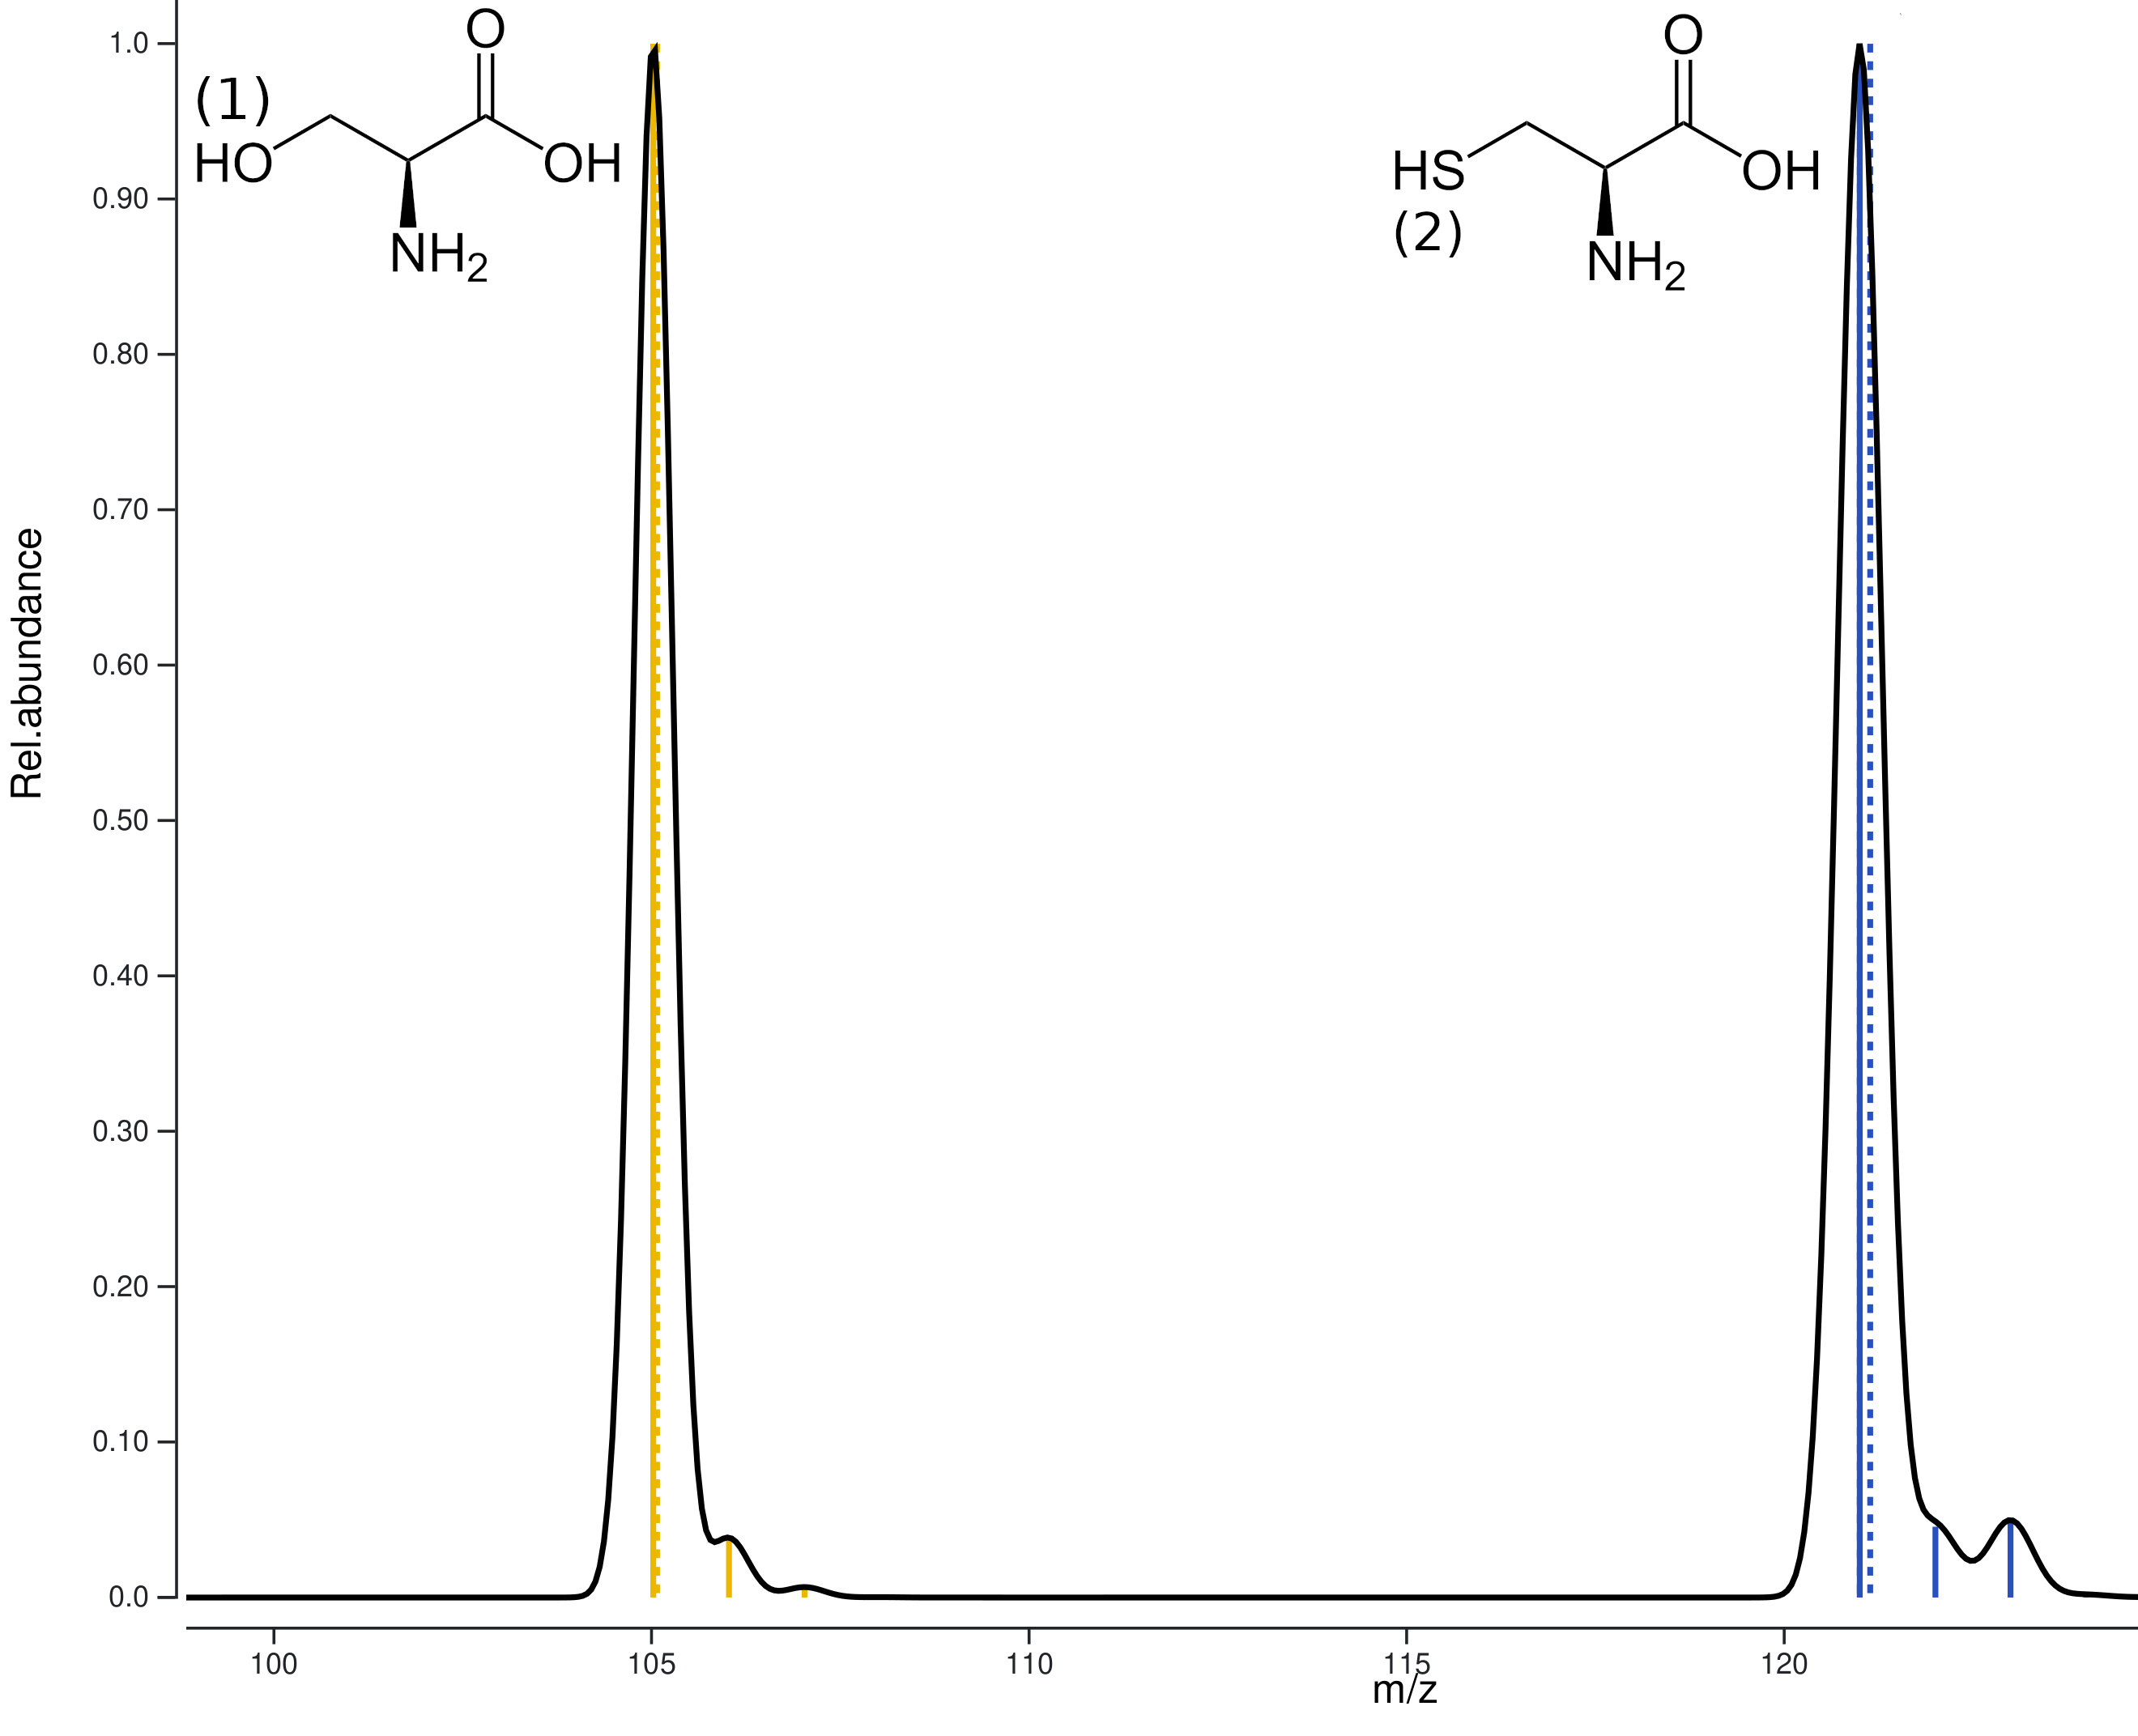
\includegraphics[width=0.75\textwidth]{./Resources/Simulated_Mass_Spectrum.png}
   \centering
   \caption{Computergeneriertes Massenspektrum von der Aminosäure \emph{Serin} (1) und \emph{Cystesin} (2). Peak von \emph{Serin} liegt bei 105; bei \emph{Systesin} um 121. y: relative Häufigkeit}
\end{figure}

Die Maxima werden \gerquot{Peaks} genannt und sind für eine Aminosäure an charakteristischer Position auf der $ x $-Achse. Obwohl sich die beiden Aminosäuren in der Abbildung \ref{fig:Sim_Mass_Spec} nur durch ein Atom unterscheiden (das linke Sauerstoffatom wurde durch ein Schwefelatom ersetzt) sind deren Massenspektren auf der $ x $-Achse weit voneinander entfernt und machen die beiden Aminosäuren dadurch sicher unterscheidbar.\\

Bei einzelnen Aminosäuren funktioniert die MS zuverlässig; bei Peptiden allerdings steht man vor dem Problem, dass das Massenspektrum unübersichtlicher wird und auch Peaks, die von Hintergrundrauschen stammen, schwerer herausgefiltert werden können. Abhilfe schafft hier die Tandem-Massenspektrometrie.

\subsection{Tandem-Massenspektrometrie (MS/MS)}\label{ss:Tandem_MS}
Bei der Tandem-Massenspektrometrie (MS/MS oder MS2) werden zwei MS Vorgänge hintereinander mit einer Probe durchgeführt. Die erste MS dient dazu Ionen aus einem bestimmten \massCharge Bereich auswählbar zu machen. Es entspricht also quasi einer Form der Filterung.

Vor der 2. MS werden die ausgewählten Reste einer Fragmentierung unterzogen. Bei einer Fragmentierung führt man Energie zu mit dem Ziel, dass die Ionen zerfallen und sog. Fragment-Ionen bilden. Diese Fragment-Ionen werden dann auf dem Massenspektrum nach der 2. MS sichtbar gemacht.

Fragment-Ionen sind kleiner als die ursprünglichen Ionen. So kann die 2. MS mit einer höheren Selektivität durchgeführt werden, welches Peaks durch Hintergrundrauschen verringert. Auch lassen sich Ionen besser identifizieren, die ein sehr ähnliches \massCharge-Verhältnis besitzen. Nach der 2. MS liegt eine Fülle an Fragment-Ionen-Peaks vor, aus denen sich die ursprünglichen Strukturinformationen ableiten lassen, da Ionen in spezifische Fragmente zerfallen \cite{Gross2013}. Zusammengefasst kann man sagen, dass das MS/MS Verfahren Ergebnisse höherer Güte erzeugt im Vergleich zur einfachen MS.

\section{De-Novo-Peptidsequenzierung mit \emph{pNovo+}}\label{s:pNovoPlusSeq}
Die \emph{pNovo+} Methode ist eine \gls{gls:DeNovo}, die mit einem \gls{gls:SpecGraph}en für die Auswertung der MS2-Spektren arbeitet und eine Erweiterung des \emph{pNovo} Verfahren darstellt \cite{pNovo}. Der Hauptansatz ist, dass zwei MS/MS Durchläufe mit jeweils verschiedenen Fragmentierungsmethoden\footnote{\emph{pNovo+} verwendet die higher energy
collisional dissociation (HCD) und die electron transfer dissociation (ETD) Fragmentierungsmethoden.} durchgeführt werden. Durch die Wahl einer anderen Fragmentierungsmethode ändert sich auch das MS2-Spektrum. Wenn nun Fragmentierungsmethoden verwendet werden, die möglichst komplementäre Spektren erzeugen, dann lässt sich durch das Zusammenführen der beiden MS2-Spektren die Qualität der Ergebnisse verbessern. Zum Beispiel lassen sich dadurch viele Peaks, die vom Hintergrundrauschen stammen, entfernen.

Für die Ermittlung der Sequenz eines Peptides wird zunächst ein Spektrums-Graph gebildet \dashAndSpace in Form eines DAG (directed acyclic graph). In diesem Graphen wird dann der längste Pfad bei gegebenen Start- und Endknoten berechnet. Die Reihenfolge der Knoten, die im längsten Pfad durchlaufen werden, stellt dann die Peptidsequenz dar.

\subsection{Vorverarbeitung der MS2-Spektren}\label{ss:Vorverarbeitung}
Bevor aus den MS2-Spektren der Spektrums-Graph gebildet werden kann, müssen die Daten vorverarbeitet werden. Für die Auswertung ist es von entscheidener Bedeutung, dass möglichst wenig Peaks verwendet werden, die vom Hintergrundrauschen stammen. Im weiteren Verlauf werden an einem exemplarischen MS2-Spektrum die Verarbeitungsschritte dargestellt.\\

Der erste Schritt ist das Verwenden des natürlichen Logarithmus der Intensitäten. Die Idee dabei ist, dass Hintergrundrauschen nicht überpriorisiert wird.

\begin{figure}[H]
   \centering
   \begin{minipage}[t]{.45\linewidth}
      \centering
      \begin{tikzpicture}[scale=\tikzScale, baseline=(current bounding box.center)]
         \draw [<->,thick] (0,\yAxisHeight) node (yaxis) [above] {\yAxisUnit}
         |- (\xAxisLength,0) node (xaxis) [right] {\xAxisUnit};
\draw[thick] (0.2, 0.0) -- (0.2, 2.3);
\draw[thick] (0.382, 0.0) -- (0.382, 1.7);
\draw[thick] (0.476, 0.0) -- (0.476, 2.7);
\draw[thick] (0.456, 0.0) -- (0.456, 1.8);
\draw[thick] (0.6859999999999999, 0.0) -- (0.6859999999999999, 2.7);
\draw[thick] (0.6839999999999999, 0.0) -- (0.6839999999999999, 1.8);
\draw[thick] (0.752, 0.0) -- (0.752, 1.1);
\draw[thick] (0.8200000000000001, 0.0) -- (0.8200000000000001, 2.2);
\draw[thick] (1.076, 0.0) -- (1.076, 1.5);
\draw[thick] (1.16, 0.0) -- (1.16, 1.9);
\draw[thick] (1.2120000000000002, 0.0) -- (1.2120000000000002, 2.0);
\draw[thick] (1.28, 0.0) -- (1.28, 1.9);
\draw[thick] (1.452, 0.0) -- (1.452, 1.3);
\draw[thick] (1.426, 0.0) -- (1.426, 1.9);
\draw[thick] (1.548, 0.0) -- (1.548, 1.9);
\draw[thick] (1.6740000000000002, 0.0) -- (1.6740000000000002, 1.5);
\draw[thick] (1.788, 0.0) -- (1.788, 2.5);
\draw[thick] (1.856, 0.0) -- (1.856, 2.3);
\draw[thick] (2.036, 0.0) -- (2.036, 1.7);
\draw[thick] (2.142, 0.0) -- (2.142, 1.6);
\draw[thick] (2.2520000000000002, 0.0) -- (2.2520000000000002, 2.0);
\draw[thick] (2.386, 0.0) -- (2.386, 1.6);
\draw[thick] (2.488, 0.0) -- (2.488, 2.9);
\draw[thick] (2.4739999999999998, 0.0) -- (2.4739999999999998, 2.7);
\draw[thick] (2.504, 0.0) -- (2.504, 2.0);
\draw[thick] (2.682, 0.0) -- (2.682, 2.0);
\draw[thick] (2.702, 0.0) -- (2.702, 2.5);
\draw[thick] (2.9259999999999997, 0.0) -- (2.9259999999999997, 2.8);
\draw[thick] (3.024, 0.0) -- (3.024, 2.4);
\draw[thick] (3.096, 0.0) -- (3.096, 1.8);
\draw[thick] (3.244, 0.0) -- (3.244, 2.6);
\draw[thick] (3.362, 0.0) -- (3.362, 1.9);
\draw[thick] (3.46, 0.0) -- (3.46, 2.3);
\draw[thick] (3.516, 0.0) -- (3.516, 1.1);
\draw[thick] (3.584, 0.0) -- (3.584, 1.8);
\draw[thick] (3.652, 0.0) -- (3.652, 2.0);
\draw[thick] (3.838, 0.0) -- (3.838, 1.5);
\draw[thick] (3.8819999999999997, 0.0) -- (3.8819999999999997, 2.6);
\draw[thick] (4.088, 0.0) -- (4.088, 2.6);
\draw[thick] (4.046, 0.0) -- (4.046, 1.1);
\draw[thick] (4.167999999999999, 0.0) -- (4.167999999999999, 2.0);
\draw[thick] (4.266, 0.0) -- (4.266, 2.4);
\draw[thick] (4.38, 0.0) -- (4.38, 1.1);
\draw[thick] (4.456, 0.0) -- (4.456, 2.2);
\draw[thick] (4.644, 0.0) -- (4.644, 2.6);
\draw[thick] (4.675999999999999, 0.0) -- (4.675999999999999, 2.5);
\draw[thick] (4.898000000000001, 0.0) -- (4.898000000000001, 1.2);
   \end{tikzpicture}%
   \end{minipage}%
   \textbf{$\rightarrow$} 
   \begin{minipage}[t]{.45\linewidth}
      \centering
      \begin{tikzpicture}[scale=\tikzScale, baseline=(current bounding box.center)]
      \draw [<->,thick] (0,\yAxisHeight) node (yaxis) [above] {\yAxisUnit}
      |- (\xAxisLength,0) node (xaxis) [right] {\xAxisUnit};
\draw[thick] (0.2, 0.0) -- (0.2, {ln(2.3)});
\draw[thick] (0.382, 0.0) -- (0.382, {ln(1.7)});
\draw[thick] (0.476, 0.0) -- (0.476, {ln(2.7)});
\draw[thick] (0.456, 0.0) -- (0.456, {ln(1.8)});
\draw[thick] (0.6859999999999999, 0.0) -- (0.6859999999999999, {ln(2.7)});
\draw[thick] (0.6839999999999999, 0.0) -- (0.6839999999999999, {ln(1.8)});
\draw[thick] (0.752, 0.0) -- (0.752, {ln(1.1)});
\draw[thick] (0.8200000000000001, 0.0) -- (0.8200000000000001, {ln(2.2)});
\draw[thick] (1.076, 0.0) -- (1.076, {ln(1.5)});
\draw[thick] (1.16, 0.0) -- (1.16, {ln(1.9)});
\draw[thick] (1.2120000000000002, 0.0) -- (1.2120000000000002, {ln(2.0)});
\draw[thick] (1.28, 0.0) -- (1.28, {ln(1.9)});
\draw[thick] (1.452, 0.0) -- (1.452, {ln(1.3)});
\draw[thick] (1.426, 0.0) -- (1.426, {ln(1.9)});
\draw[thick] (1.548, 0.0) -- (1.548, {ln(1.9)});
\draw[thick] (1.6740000000000002, 0.0) -- (1.6740000000000002, {ln(1.5)});
\draw[thick] (1.788, 0.0) -- (1.788, {ln(2.5)});
\draw[thick] (1.856, 0.0) -- (1.856, {ln(2.3)});
\draw[thick] (2.036, 0.0) -- (2.036, {ln(1.7)});
\draw[thick] (2.142, 0.0) -- (2.142, {ln(1.6)});
\draw[thick] (2.2520000000000002, 0.0) -- (2.2520000000000002, {ln(2.0)});
\draw[thick] (2.386, 0.0) -- (2.386, {ln(1.6)});
\draw[thick] (2.488, 0.0) -- (2.488, {ln(2.9)});
\draw[thick] (2.4739999999999998, 0.0) -- (2.4739999999999998, {ln(2.7)});
\draw[thick] (2.504, 0.0) -- (2.504, {ln(2.0)});
\draw[thick] (2.682, 0.0) -- (2.682, {ln(2.0)});
\draw[thick] (2.702, 0.0) -- (2.702, {ln(2.5)});
\draw[thick] (2.9259999999999997, 0.0) -- (2.9259999999999997, {ln(2.8)});
\draw[thick] (3.024, 0.0) -- (3.024, {ln(2.4)});
\draw[thick] (3.096, 0.0) -- (3.096, {ln(1.8)});
\draw[thick] (3.244, 0.0) -- (3.244, {ln(2.6)});
\draw[thick] (3.362, 0.0) -- (3.362, {ln(1.9)});
\draw[thick] (3.46, 0.0) -- (3.46, {ln(2.3)});
\draw[thick] (3.516, 0.0) -- (3.516, {ln(1.1)});
\draw[thick] (3.584, 0.0) -- (3.584, {ln(1.8)});
\draw[thick] (3.652, 0.0) -- (3.652, {ln(2.0)});
\draw[thick] (3.838, 0.0) -- (3.838, {ln(1.5)});
\draw[thick] (3.8819999999999997, 0.0) -- (3.8819999999999997, {ln(2.6)});
\draw[thick] (4.088, 0.0) -- (4.088, {ln(2.6)});
\draw[thick] (4.046, 0.0) -- (4.046, {ln(1.1)});
\draw[thick] (4.167999999999999, 0.0) -- (4.167999999999999, {ln(2.0)});
\draw[thick] (4.266, 0.0) -- (4.266, {ln(2.4)});
\draw[thick] (4.38, 0.0) -- (4.38, {ln(1.1)});
\draw[thick] (4.456, 0.0) -- (4.456, {ln(2.2)});
\draw[thick] (4.644, 0.0) -- (4.644, {ln(2.6)});
\draw[thick] (4.675999999999999, 0.0) -- (4.675999999999999, {ln(2.5)});
\draw[thick] (4.898000000000001, 0.0) -- (4.898000000000001, {ln(1.2)});
      \end{tikzpicture}
      \end{minipage}
      \caption{Anwendung des $ ln $ auf einem exemplarischen MS2-Spektrum.}
\end{figure}

Für das Verständnis des nächsten Schrittes muss man sich in Erinnerung rufen, dass eine gleiche Aminosäure keineswegs immer die gleiche Masse hat. Durch Isotope existiert eine gewisse \gerquot{Massenbandbreite} für ein und dieselbe Aminosäure. MS Systeme sind heute so genau, dass sie diese Differenzen erkennen. Dies hat den ungewollten Effekt, dass mehrere Peaks zu einer Aminosäure gehören können \cite{IsotopicDistributionMS}. Gleichzeitig können die \gerquot{Massenbandbreiten} zweier Aminosäuren sich überschneiden, sodass im ungünstigen Fall zwei Peaks kaum unterscheidbar nebeneinander liegen.\\

Eine Möglichkeit mit dieser Problematik umzugehen ist die Verwendung der monoisotopischen Masse. Die monoisotopische Masse ist die \gerquot{[...] exact mass of the most abundant naturally occurring stable isotope determined relative to the mass of 12 C, which is assigned the exact value of 12.0000.} \cite{MonoisotopicMass}. Ohne dabei jetzt tiefer ins Detail zu gehen kann man sagen, dass alle Peaks, deren Intensität mit einer möglichen monoisotopischen Masse übereinstimmen, auf jeden Fall einer Aminosäure entsprechen und (höchstwahrscheinlich)\footnote{Natürlich ist es möglich, dass das Rauschen zufällig einer monoisotopischen Masse entspricht. Die Wahrscheinlichkeit dafür ist allerdings sehr gering.} kein Hintergrundrauschen sind \cite{MassDefectMS}. Diese Peaks bekommen eine sogennante \emph{charge state}.\\

Der Algorithmus verwendet die \emph{charge state} Peaks als Ausganspunkte für weitere Berechnungen. Wenn die \massCharge Differenz zu einem anderen Peak einem Peptidfragment entspricht, dann stammt dieser Peak höchstwahrscheinlich von einem Fragment. Insgesamt werden damit die relevanten Peptidfragmente herausgeholt. Abbildung \ref{MonoisotopicMassFiltering} zeigt das Ergebnis nach den beiden zuvor genannten Schritten.

\begin{figure}[H]\label{MonoisotopicMassFiltering}
   \centering
   \begin{minipage}[t]{.45\linewidth}
      \centering
      \begin{tikzpicture}[scale=\tikzScale, baseline=(current bounding box.center)]
         \draw [<->,thick] (0,\yAxisHeight) node (yaxis) [above] {\yAxisUnit}
         |- (\xAxisLength,0) node (xaxis) [right] {\xAxisUnit};
\draw[thick] (0.2, 0.0) -- (0.2, {ln(2.3)});
\draw[color=blue!85!,opacity=.55,thick] (0.382, 0.0) -- (0.382, {ln(1.7)});
\draw[color=blue!85!,opacity=.55,thick] (0.476, 0.0) -- (0.476, {ln(2.7)});
\draw[color=magenta,thick] (0.456, 0.0) -- (0.456, {ln(1.8)});
\draw[color=blue!85!,opacity=.55,thick] (0.6859999999999999, 0.0) -- (0.6859999999999999, {ln(2.7)});
\draw[color=blue!85!,opacity=.55,thick] (0.6839999999999999, 0.0) -- (0.6839999999999999, {ln(1.8)});
\draw[thick] (0.752, 0.0) -- (0.752, {ln(1.1)});
\draw[thick] (0.8200000000000001, 0.0) -- (0.8200000000000001, {ln(2.2)});
\draw[thick] (1.076, 0.0) -- (1.076, {ln(1.5)});
\draw[thick] (1.16, 0.0) -- (1.16, {ln(1.9)});
\draw[thick] (1.2120000000000002, 0.0) -- (1.2120000000000002, {ln(2.0)});
\draw[thick] (1.28, 0.0) -- (1.28, {ln(1.9)});
\draw[color=blue!85!,opacity=.55,thick] (1.452, 0.0) -- (1.452, {ln(1.3)});
\draw[color=blue!85!,opacity=.55,thick] (1.426, 0.0) -- (1.426, {ln(1.9)});
\draw[color=magenta,thick] (1.548, 0.0) -- (1.548, {ln(1.9)});
\draw[color=blue!85!,opacity=.55,thick] (1.6740000000000002, 0.0) -- (1.6740000000000002, {ln(1.5)});
\draw[color=blue!85!,opacity=.55,thick] (1.788, 0.0) -- (1.788, {ln(2.5)});
\draw[thick] (1.856, 0.0) -- (1.856, {ln(2.3)});
\draw[thick] (2.036, 0.0) -- (2.036, {ln(1.7)});
\draw[thick] (2.142, 0.0) -- (2.142, {ln(1.6)});
\draw[thick] (2.2520000000000002, 0.0) -- (2.2520000000000002, {ln(2.0)});
\draw[thick] (2.386, 0.0) -- (2.386, {ln(1.6)});
\draw[color=blue!85!,opacity=.55,thick] (2.488, 0.0) -- (2.488, {ln(2.9)});
\draw[thick] (2.4739999999999998, 0.0) -- (2.4739999999999998, {ln(2.7)});
\draw[color=blue!85!,opacity=.55,thick] (2.504, 0.0) -- (2.504, {ln(2.0)});
\draw[color=magenta,thick] (2.682, 0.0) -- (2.682, {ln(2.0)});
\draw[color=blue!85!,opacity=.55,thick] (2.702, 0.0) -- (2.702, {ln(2.5)});
\draw[thick] (2.9259999999999997, 0.0) -- (2.9259999999999997, {ln(2.8)});
\draw[thick] (3.024, 0.0) -- (3.024, {ln(2.4)});
\draw[thick] (3.096, 0.0) -- (3.096, {ln(1.8)});
\draw[thick] (3.244, 0.0) -- (3.244, {ln(2.6)});
\draw[thick] (3.362, 0.0) -- (3.362, {ln(1.9)});
\draw[color=blue!85!,opacity=.55,thick] (3.46, 0.0) -- (3.46, {ln(2.3)});
\draw[color=blue!85!,opacity=.55,thick] (3.516, 0.0) -- (3.516, {ln(1.1)});
\draw[color=blue!85!,opacity=.55,thick] (3.584, 0.0) -- (3.584, {ln(1.8)});
\draw[color=magenta,thick] (3.652, 0.0) -- (3.652, {ln(2.0)});
\draw[color=blue!85!,opacity=.55,thick] (3.838, 0.0) -- (3.838, {ln(1.5)});
\draw[color=blue!85!,opacity=.55,thick] (3.8819999999999997, 0.0) -- (3.8819999999999997, {ln(2.6)});
\draw[thick] (4.088, 0.0) -- (4.088, {ln(2.6)});
\draw[thick] (4.046, 0.0) -- (4.046, {ln(1.1)});
\draw[thick] (4.167999999999999, 0.0) -- (4.167999999999999, {ln(2.0)});
\draw[thick] (4.266, 0.0) -- (4.266, {ln(2.4)});
\draw[color=blue!85!,opacity=.55,thick] (4.38, 0.0) -- (4.38, {ln(1.1)});
\draw[color=blue!85!,opacity=.55,thick] (4.456, 0.0) -- (4.456, {ln(2.2)});
\draw[color=magenta,thick] (4.644, 0.0) -- (4.644, {ln(2.6)});
\draw[color=blue!85!,opacity=.55,thick] (4.675999999999999, 0.0) -- (4.675999999999999, {ln(2.5)});
\draw[color=blue!85!,opacity=.55,thick] (4.898000000000001, 0.0) -- (4.898000000000001, {ln(1.2)});
   \end{tikzpicture}%
   \end{minipage}%
   \textbf{$\rightarrow$} 
   \begin{minipage}[t]{.45\linewidth}
      \centering
      \begin{tikzpicture}[scale=\tikzScale, baseline=(current bounding box.center)]
      \draw [<->,thick] (0,\yAxisHeight) node (yaxis) [above] {\yAxisUnit}
      |- (\xAxisLength,0) node (xaxis) [right] {\xAxisUnit};
\draw[color=blue!85!,opacity=.55,thick] (0.382, 0.0) -- (0.382, {ln(1.7)});
\draw[color=blue!85!,opacity=.55,thick] (0.476, 0.0) -- (0.476, {ln(2.7)});
\draw[color=magenta,thick] (0.456, 0.0) -- (0.456, {ln(1.8)});
\draw[color=blue!85!,opacity=.55,thick] (0.6859999999999999, 0.0) -- (0.6859999999999999, {ln(2.7)});
\draw[color=blue!85!,opacity=.55,thick] (0.6839999999999999, 0.0) -- (0.6839999999999999, {ln(1.8)});
\draw[color=blue!85!,opacity=.55,thick] (1.452, 0.0) -- (1.452, {ln(1.3)});
\draw[color=blue!85!,opacity=.55,thick] (1.426, 0.0) -- (1.426, {ln(1.9)});
\draw[color=magenta,thick] (1.548, 0.0) -- (1.548, {ln(1.9)});
\draw[color=blue!85!,opacity=.55,thick] (1.6740000000000002, 0.0) -- (1.6740000000000002, {ln(1.5)});
\draw[color=blue!85!,opacity=.55,thick] (1.788, 0.0) -- (1.788, {ln(2.5)});
\draw[color=blue!85!,opacity=.55,thick] (2.488, 0.0) -- (2.488, {ln(2.9)});
\draw[color=blue!85!,opacity=.55,thick] (2.504, 0.0) -- (2.504, {ln(2.0)});
\draw[color=magenta,thick] (2.682, 0.0) -- (2.682, {ln(2.0)});
\draw[color=blue!85!,opacity=.55,thick] (2.702, 0.0) -- (2.702, {ln(2.5)});
\draw[color=blue!85!,opacity=.55,thick] (3.46, 0.0) -- (3.46, {ln(2.3)});
\draw[color=blue!85!,opacity=.55,thick] (3.516, 0.0) -- (3.516, {ln(1.1)});
\draw[color=blue!85!,opacity=.55,thick] (3.584, 0.0) -- (3.584, {ln(1.8)});
\draw[color=magenta,thick] (3.652, 0.0) -- (3.652, {ln(2.0)});
\draw[color=blue!85!,opacity=.55,thick] (3.838, 0.0) -- (3.838, {ln(1.5)});
\draw[color=blue!85!,opacity=.55,thick] (3.8819999999999997, 0.0) -- (3.8819999999999997, {ln(2.6)});
\draw[color=blue!85!,opacity=.55,thick] (4.38, 0.0) -- (4.38, {ln(1.1)});
\draw[color=blue!85!,opacity=.55,thick] (4.456, 0.0) -- (4.456, {ln(2.2)});
\draw[color=magenta,thick] (4.644, 0.0) -- (4.644, {ln(2.6)});
\draw[color=blue!85!,opacity=.55,thick] (4.675999999999999, 0.0) -- (4.675999999999999, {ln(2.5)});
\draw[color=blue!85!,opacity=.55,thick] (4.898000000000001, 0.0) -- (4.898000000000001, {ln(1.2)});
      \end{tikzpicture}
      \end{minipage}
      \caption{Entfernen von Peaks, die keiner monoisotopischen Masse entsprechen oder benachbart mit einer Differenz von einem Fragment-Ion sind.}
\end{figure}

Tatsächlich ist die Verarbeitung an dieser Stelle noch etwas komplexer. So existieren auch noch sogenannte \emph{isotopic cluster}\footnote{Definition eines \emph{isotopic cluster} nach IUPAC: \gerquot{Group of peaks representing ions of the same elemental composition, but different isotopic compositions.} \cite[1556]{IUPACDefinitions}}, die gesondert verarbeitet werden. Für das grundsätzliche Prinzip ist dieses Detail allerdings weniger relevant.\\

Im letzten Vorberarbeitungsschritt werden Peaks aus einem irrelevanten \massCharge Bereich entfernt und naheliegende Peaks werden zusammengefasst, indem der Mittelwert sowol des \massCharge Wertes als auch der der Intensität besimmt wird. Üblicherweise liegt der Bereich für das Zusammenfassen bei $ +- 20 ppm $.

\begin{figure}[H]
   \centering
   \begin{minipage}[t]{.45\linewidth}
      \centering
      \begin{tikzpicture}[scale=\tikzScale, baseline=(current bounding box.center)]
         \draw [<->,thick] (0,\yAxisHeight) node (yaxis) [above] {\yAxisUnit}
         |- (\xAxisLength,0) node (xaxis) [right] {\xAxisUnit};
\draw[thick] (0.382, 0.0) -- (0.382, {ln(1.7)});
\draw[thick] (0.476, 0.0) -- (0.476, {ln(2.7)});
\draw[thick] (0.456, 0.0) -- (0.456, {ln(1.8)});
\draw[thick] (0.6859999999999999, 0.0) -- (0.6859999999999999, {ln(2.7)});
\draw[thick] (0.6839999999999999, 0.0) -- (0.6839999999999999, {ln(1.8)});
\draw[color=red,thick] (1.452, 0.0) -- (1.452, {ln(1.3)});
\draw[color=red,thick] (1.426, 0.0) -- (1.426, {ln(1.9)});
\draw[thick] (1.548, 0.0) -- (1.548, {ln(1.9)});
\draw[thick] (1.6740000000000002, 0.0) -- (1.6740000000000002, {ln(1.5)});
\draw[thick] (1.788, 0.0) -- (1.788, {ln(2.5)});
\draw[color=red,thick] (2.488, 0.0) -- (2.488, {ln(2.9)});
\draw[color=red,thick] (2.504, 0.0) -- (2.504, {ln(2.0)});
\draw[color=red,thick] (2.682, 0.0) -- (2.682, {ln(2.0)});
\draw[color=red,thick] (2.702, 0.0) -- (2.702, {ln(2.5)});
\draw[thick] (3.46, 0.0) -- (3.46, {ln(2.3)});
\draw[thick] (3.516, 0.0) -- (3.516, {ln(1.1)});
\draw[thick] (3.584, 0.0) -- (3.584, {ln(1.8)});
\draw[thick] (3.652, 0.0) -- (3.652, {ln(2.0)});
\draw[color=red,thick] (3.838, 0.0) -- (3.838, {ln(1.5)});
\draw[color=red,thick] (3.8819999999999997, 0.0) -- (3.8819999999999997, {ln(2.6)});
\draw[thick] (4.38, 0.0) -- (4.38, {ln(1.1)});
\draw[thick] (4.456, 0.0) -- (4.456, {ln(2.2)});
\draw[thick] (4.644, 0.0) -- (4.644, {ln(2.6)});
\draw[thick] (4.675999999999999, 0.0) -- (4.675999999999999, {ln(2.5)});
\draw[thick] (4.898000000000001, 0.0) -- (4.898000000000001, {ln(1.2)});

\fill[red!25!,opacity=.25] (0,0) rectangle (1,\yAxisHeight-\axisColorOffset);
         \fill[red!25!,opacity=.25] (\xAxisLength-1,0) rectangle (\xAxisLength-\axisColorOffset,\yAxisHeight-\axisColorOffset);
         \fill[green!25!,opacity=.25] (1,0) rectangle (\xAxisLength-1,\yAxisHeight-\axisColorOffset);
   \end{tikzpicture}%
   \end{minipage}%
   \textbf{$\rightarrow$} 
   \begin{minipage}[t]{.45\linewidth}
      \centering
      \begin{tikzpicture}[scale=\tikzScale, baseline=(current bounding box.center)]
      \draw [<->,thick] (0,\yAxisHeight) node (yaxis) [above] {\yAxisUnit}
      |- (\xAxisLength,0) node (xaxis) [right] {\xAxisUnit};
%\draw[color=red,thick] (1.452, 0.0) -- (1.452, {ln(1.3)});
%\draw[color=red,thick] (1.426, 0.0) -- (1.426, {ln(1.9)});
\draw[color=red,ultra thick] ({(1.452+1.426)/2}, 0.0) -- ({(1.452+1.426)/2}, {(ln(1.3)+ln(1.9))/2});

\draw[thick] (1.548, 0.0) -- (1.548, {ln(1.9)});
\draw[thick] (1.6740000000000002, 0.0) -- (1.6740000000000002, {ln(1.5)});
\draw[thick] (1.788, 0.0) -- (1.788, {ln(2.5)});

%\draw[color=red,thick] (2.488, 0.0) -- (2.488, {ln(2.9)});
%\draw[color=red,thick] (2.504, 0.0) -- (2.504, {ln(2.0)});
\draw[color=red,ultra thick] ({(2.488+2.504)/2}, 0.0) -- ({(2.488+2.504)/2}, {(ln(2.9)+ln(2.0))/2});

%\draw[color=red,thick] (2.682, 0.0) -- (2.682, {ln(2.0)});
%\draw[color=red,thick] (2.702, 0.0) -- (2.702, {ln(2.5)});
\draw[color=red,ultra thick] ({(2.682+2.702)/2}, 0.0) -- ({(2.682+2.702)/2}, {(ln(2.0+ln(2.5))/2});

\draw[thick] (3.46, 0.0) -- (3.46, {ln(2.3)});
\draw[thick] (3.516, 0.0) -- (3.516, {ln(1.1)});
\draw[thick] (3.584, 0.0) -- (3.584, {ln(1.8)});
\draw[thick] (3.652, 0.0) -- (3.652, {ln(2.0)});

%\draw[color=red,thick] (3.838, 0.0) -- (3.838, {ln(1.5)});
%\draw[color=red,thick] (3.8819999999999997, 0.0) -- (3.8819999999999997,{ln(2.6)});
\draw[color=red,ultra thick] ({(3.838+3.8819999999999997)/2}, 0.0) -- ({(3.838+3.8819999999999997)/2}, {(ln(1.5)+ln(2.6))/2});

\fill[red!25!,opacity=.25] (0,0) rectangle (1,\yAxisHeight-\axisColorOffset);
         \fill[red!25!,opacity=.25] (\xAxisLength-1,0) rectangle (\xAxisLength-\axisColorOffset,\yAxisHeight-\axisColorOffset);
         \fill[green!25!,opacity=.25] (1,0) rectangle (\xAxisLength-1,\yAxisHeight-\axisColorOffset);
      \end{tikzpicture}
      \end{minipage}
      \caption{Entfernen von Peaks aus einem irrelevanten \massCharge Bereich und zusammenfassen naheliegender Peaks. Rot markierte Peaks sind jene, die zusammengefasst werden.}
\end{figure}

\subsection{Bildung eines Spektrums-Graphen}\label{ss:BildungSpekGraph}
Der Spektrums-Graph wird aus einem vorverarbeiteten MS2-Spektrum (siehe Kapitel: \ref{ss:Vorverarbeitung}) gebildet. Im initialen Zustand werden die Peaks als Knoten interpretiert. Dazu kommt ein Start- und Endknoten. Jedem Knoten wird eine Masse zugeordet; im initialen Zustand bekommt der Startknoten die Masse 0 und der Endknoten die Masse des vorherigen Knotens minus der Masse des Wassers ($ 18,02 $). Die Masse der übrigen Knoten entsprechen ihren jeweils korrespondierenden \massCharge Wert. Die gerichteten Kanten werden zwischen einem Knotenpaar hinzugefügt, wenn die Differenz deren Masse gleich ist mit der Masse von ein oder zwei Aminosäuren.

\subsection{Identifikation der Aminosäuresequenz}
Der gebildete DAG kann mit klassischen Algorithmen, die den längsten Pfad suchen, durchlaufen werden. Bezogen auf die Graphentheorie entspricht die Ermittlung der Aminosäurensequenz dem Suchen eines bestimmten Pfades \dashAndSpace und nicht nach irgendeinem Pfad. Daher muss der Algorithmus mittels einer Breitensuche arbeiten, um alle möglichen Pfade zu bestimmen.

In aller Regel wird es mehrere Pfade geben. Bestimmte Sequenzen sind wahrscheinlicher als andere. So sind Pfade mit Kanten, die wegen der Massendifferenz von genau einer Aminosäure gebildet wurden, wahrscheinlicher \cite{pNovoPlus}. Alle Pfade bekommen mittels einer Scoring-Funktion einen Wert zugewiesen. Der Pfad mit dem höchsten Scoring-Wert ist wahrscheinlich das richtige Ergebnis. Die Scoring-Funktion berücksichtigt unter anderem wie viele Fragmente, die einer bestimmten Aminosäure zugeordet werden können, im MS2-Spektrum vorhanden sind \cite{pNovo}. Die Sequenz mit dem höchsten Scoring-Wert ist das Endergebnis.

\section{De-Novo-Peptidsequenzierung mit \emph{Open-pNovo}}\label{s:OpenpNovoSeq}
Bei Proteinen können posttranslationale Proteinmodifikationen (PTM) auftreten. PTMs sind Ereignisse, bei denen sich Änderungen im Protein einstellen \cite{Mann2003}; teilweise sind die Änderungen von einer Zelle erwünscht \dashAndSpace teilweise stammen sie aber auch zum Beispiel von unerwünschten Wechselwirkungen nebeneinanderliegenden Aminosäuren. Ein Teil dieser PTMs führen zu einer Änderung der Aminosäuresequenz. Dies ist für die \gls{gls:DeNovo} nicht weiter problematisch, da sowieso ohne eine Datenbank gearbeitet wird, sodass solche PTMs nicht einmal auffallen würden. Andere PTMs hingegen haben die Auswirkung, dass Stoffe gebildet werden, die nicht mehr zu der Gruppe der proteinogenen Aminosäuren gehören. Proteinogene Aminosäuren sind jene Aminosäuren, die für den Bau von Proteinen verwendet werden. Der Effekt ist also, dass Stoffe (oder deren Fragmente) bei einem Massenspektrum angezeigt werden, die kein Teil eines Peptids sein können. Bei der Sequenzierung von Peptidfragmenten muss dies daher berücksichtigt werden.
Wenn im weiteren Verlauf von PTMs gesprochen wird, dann sind solche gemeint, die für die \gls{gls:DeNovo} relevant sind.

Open-pNovo ist ein \gls{gls:DeNovo}sverfahren, welches auf pNovo+ Tool aufbaut und versucht die Problematik mit den PTMs zu lösen.

\subsection{PTMs im konstruierten DAG}
Die Konvertierung eines MS2-Spektrums läuft bis zum DAG analog ab wie in den Kapiteln \ref{ss:Vorverarbeitung} und \ref{ss:BildungSpekGraph} für pNovo+. Der Unterschied ist nun, dass es zwei Arten von Kanten gibt:

\begin{itemize}
   \item \gerquot{Normale} Kanten: Kanten, die gebildet werden, wie es bereits für \emph{pNovo+} gezeigt wurde. 
   \item \gerquot{Modifizierte} Kanten: Kanten, die zum Grahpen hinzugefügt werden, wenn die Massendifferenz zweier Knoten der Masse einer Aminosäure plus der Masse einer möglichen PTM-Änderung entspricht. 
\end{itemize}

Eine Liste aller PTMs in der Datenbank Unimod (sowohl relevante als auch nicht relevante) beinhaltet aktuell 1510 Einträge\footnote{Siehe: \url{https://www.ebi.ac.uk/ols/ontologies/unimod}} (Stand: 18.04.2022). Für die modifizierten Kanten gibt es insgesamt $ 1510 * 20 = 30200 $ mögliche Differenzen, wobei viele davon nicht relevante PTMs sind. Zum Vergleich: bei den normalen Kanten gibt es $ 20^2 = 400 $ mögliche Differenzen.

Die hohe Anzahl an Differenzen für modifizierte Kanten hat die Konsequenz, dass viele Knoten zufällig verbunden werden und dass dadurch die Genauigkeit der Ergebnisse abnimmt. Dieses Problem kann man durch eine geringere Liste an möglichen PTMs abfedern, allerdings mit einem Verlust  der Genauigkeit auf Seiten der PTMs. Es ist hier also eine Abwägung.

\subsection{Evaluierung von Open-pNovo}
Open-pNovo wurde sowohl auf drei realen als auch auf drei generierten Testdaten getestet. Tabelle \ref{tab:OpenPNovoResults} zeigt die Ergebnisse im Vergleich zu pNovo+ und zwei anderen Algorithmen. Die Datensätze enthielten die am häufigsten vorkommenden PTMs.

\begin{table}[H]
    \centering
    \begin{tabular}{l|c|c|c|c}
        \toprule
        \textbf{Testdatensätze} & \textbf{Open-pNovo+} & \textbf{pNovo+} & \textbf{PEAKS} & \textbf{Novor} \\
        \midrule
        Real (20259) & $76,3 \%$ & $68,5 \%$ & $65,8 \%$ & $39,9 \%$ \\
        Generiert (17877) & $77,8 \%$ & $0,6 \%$ & $0,5 \%$ & $0,2 \%$ \\
        \bottomrule
    \end{tabular}
    \newline
    \caption{Vergleich der durchschnittlichen richtigen \gls{gls:DeNovo} Peptidsequenzierungen von Open-pNovo und anderen Algorithmen \cite[650]{OpenPNovo}.}
    \label{tab:OpenPNovoResults}
\end{table}

Die enorm schlechten Ergebnisse der anderen Algorithmen bei den generierten Testdaten ist ein Nebeneffekt des Ziels bei der Testdatengenerierung. Denn diese wurden so ausgelegt, um die Grenzen von Open-pNovo+ zu ermitteln \cite[649]{OpenPNovo}. Eine Aussagekraft haben diese Ergebnisse also nicht. Allerdings auch bei realen Testdaten zeigt sich Open-pNovo als voll konkurrenzfähig gegenüber den anderen Algorithmen.

Noch besser zeigt sich Open-pNovo, wenn der Recall Wert betrachtet wird \dashAndSpace also die Anzahl an verschiedenen PSMs, die erkannt wurden. In diesem Fall ist der Abstand zu den anderen Algorithmen deutlich größer geworden.

\begin{table}[H]
    \centering
    \begin{tabular}{l|c|c|c|c}
        \toprule
        \textbf{Testdatensätze} & \textbf{Open-pNovo+} & \textbf{pNovo+} & \textbf{PEAKS} & \textbf{Novor} \\
        \midrule
        Real (5034) & $61,6 \%$ & $31,3 \%$ & $32,0 \%$ & $13,7 \%$ \\
        \bottomrule
    \end{tabular}
    \newline
    \caption{Vergleich der durchschnittlichen Recall Werte einer \gls{gls:DeNovo} Peptidsequenzierungen von Open-pNovo und anderen Algorithmen \cite[650]{OpenPNovo}.}
    \label{tab:OpenPNovoResultsRecall}
\end{table}

\subsection{Zusammenfassung}


% Die \gls{gls:DeNovo} nutzt die sogenannte \gls{gls:TMassSpek} für die Bestimmung der Peptidsequenz. Dabei wird die physikalische Eigenschaft ausgenutzt, dass jedes Atom bzw. jedes Molekül \dashAndSpace wenn es einer \gls{gls:Ionisation} unterzogen wurde \dashAndSpace ein charakteristisches \gls{gls:MassSpek} besitzt. Das \gls{gls:MassSpek} stellt also eine Art \gerquot{Fingerabdruck} eines Moleküls dar und macht dieses ermittelbar.

% U.U. eine Beispielgrafik eines Massenspektrums hinzufuegen ...

\subsubsection{\glsentrytext{gls:TMassSpek} bei größeren Molekülen}
Bei größeren Molekülen (wie einem Protein) führt die \gls{gls:Ionisation} dazu, dass das Molekül in kleinere spezifische Ionen zerfällt (sog. Fragmentierung). Die Fragmentierungsinformationen einer \gls{gls:DeNovo} sind meist unvollständig, da fehlende Daten bei einem Fragmentierungsschritt die Güte des Endergebnisses negativ beeinflusst. Dies wird insbesondere dann ein Problem, wenn unbekannte Änderungen in einer Peptidsequenz vorhanden sind.

Um dieses Problem zu verringern können unterschiedliche Techniken parallel eingesetzt werden, welche verschiedene Fragmente erzeugen und daher auch verschiedenartige \glspl{gls:MassSpek} zur Folge haben.\footnote{Konkret: Es wird sowohl das \gls{acr:HCD} als auch das \gls{acr:ETD} Verfahren angewendet.}

\subsection{Datenaufbereitung}
Typischerweise betrachtet man die sog. \gerquot{\glspl{gls:Peak}} in den \glspl{gls:MassSpek}. Jeder \gls{gls:Peak} stellt ein unterschiedliches Ion dar. Dazu kommen Messungenauigkeiten sowie Hintergrundrauschen. Durch die hohe Anzahl an möglichen Ionen kann nicht ohne weiteres differenziert werden, welcher der \glspl{gls:Peak} von welchen Ionen erzeugt wurden und welche nicht.

% Frage an Dominik: Ist hier eine einfache Auflistung an Techniken für die Datenaufbereitung besser?
Der Algorithmus für die Datenaufbereitung berechnet den natürlichen Logarithmus von den Intensitäten der \glspl{gls:Peak}, um Hintergrundrauschen und Messungenauigkeiten nicht überzupriorisieren. Zusätzlich dazu werden \glspl{gls:Peak}, die in einem Toleranzbereich nebeneinander liegen, zusammengefasst. Am Ende werden die \glspl{gls:Peak} entfernt, bei denen bekannt ist, dass es sich nicht um relevante Ionen handeln kann. (z.B. \glspl{gls:Peak} von Isotopen)

\begin{figure}[H]
   \centering
   \begin{minipage}[t]{.4\linewidth}
      \centering
      \begin{tikzpicture}[scale=\tikzScale, baseline=(current bounding box.center)]
         \draw [<->,thick] (0,2.75) node (yaxis) [above] {\yAxisUnit}
         |- (3,0) node (xaxis) [right] {\xAxisUnit};

         \draw[thick] (0.2,0) -- (0.2,1.1);
         \draw[thick] (0.3,0) -- (0.3,1.6);
         \draw[thick] (0.6,0) -- (0.6,1.7);
         \draw[thick] (0.8,0) -- (0.8,1.2);
         \draw[thick] (1.0,0) -- (1.0,1.1);

         \draw[color=red,thick] (1.2,0) -- (1.2,2.65);
         \draw[thick] (1.4,0) -- (1.4,1.4);
         \draw[thick] (1.6,0) -- (1.6,1.2);
         \draw[thick] (1.8,0) -- (1.8,1.3);
         \draw[thick] (2.0,0) -- (2.0,1.8);

         \draw[thick] (1.1,0) -- (1.1,2.0);
         \draw[color=red,thick] (0.35,0) -- (0.35,2.25);
         \draw[thick] (1.9,0) -- (1.9,1.4);
         \draw[color=red,thick] (2.2,0) -- (2.2,2.6);
         \draw[thick] (2.5,0) -- (2.5,1.25);

         \draw[thick] (2.7,0) -- (2.7,1.1);
         \foreach \x in {1,...,6}
         {
            \draw[thick] (1.2+\x*0.05,0) -- (1.2+\x*0.05,1.0+\x*0.15);
         }
      \end{tikzpicture}%
      % \subcaption{Exemplarische Rohdaten}
   \end{minipage}%
   \textbf{$\rightarrow$}
   \begin{minipage}[t]{.4\linewidth}
      \centering
      \begin{tikzpicture}[scale=\tikzScale, baseline=(current bounding box.center)]
         \draw [<->,thick] (0,2.75) node (yaxis) [above] {\yAxisUnit}
         |- (3,0) node (xaxis) [right] {\xAxisUnit};

         \draw[thick] (0.2,0) -- (0.2,{ln(1.1)});
         \draw[thick] (0.3,0) -- (0.3,{ln(1.6)});
         \draw[thick] (0.6,0) -- (0.6,{ln(1.7)});
         \draw[thick] (0.8,0) -- (0.8,{ln(1.2)});
         \draw[thick] (1.0,0) -- (1.0,{ln(1.1)});

         \draw[color=red,thick] (1.2,0) -- (1.2,{ln(2.65)});
         \draw[thick] (1.4,0) -- (1.4,{ln(1.4)});
         \draw[thick] (1.6,0) -- (1.6,{ln(1.2)});
         \draw[thick] (1.8,0) -- (1.8,{ln(1.3)});
         \draw[thick] (2.0,0) -- (2.0,{ln(1.8)});

         \draw[thick] (1.1,0) -- (1.1,{ln(2.0)});
         \draw[color=red,thick] (0.35,0) -- (0.35,{ln(2.25)});
         \draw[thick] (1.9,0) -- (1.9,{ln(1.4)});
         \draw[color=red,thick] (2.2,0) -- (2.2,{ln(2.6)});
         \draw[thick] (2.5,0) -- (2.5,{ln(1.25)});

         \draw[thick] (2.7,0) -- (2.7,{ln(1.1)});
         \foreach \x in {1,...,6}
         {%
            \draw[thick] (1.2+\x*0.05,0) -- (1.2+\x*0.05,{ln(1.0+\x*0.15)});
         }
      \end{tikzpicture}
      %\subcaption{Exemplarische Rohdaten}
   \end{minipage}
   \caption{Anwendung des $ln$ auf Rohdaten. Rote \glspl{gls:Peak} stellen hier exemplarisch fehlerhafte Daten dar, die nach dem $ln$ reduziert wurden.}
\end{figure}

\begin{figure}[H]
   \centering
   \begin{minipage}[t]{.4\linewidth}
      \centering
      \begin{tikzpicture}[scale=\tikzScale, baseline=(current bounding box.center)]
         \draw [<->,thick] (0,2.75) node (yaxis) [above] {\yAxisUnit}
         |- (3,0) node (xaxis) [right] {\xAxisUnit};

         \draw[thick] (0.2,0) -- (0.2,{ln(1.1)});
         \draw[thick] (0.3,0) -- (0.3,{ln(1.6)});
         \draw[thick] (0.6,0) -- (0.6,{ln(1.7)});
         \draw[thick] (0.8,0) -- (0.8,{ln(1.2)});
         \draw[thick] (1.0,0) -- (1.0,{ln(1.1)});

         \draw[thick] (1.2,0) -- (1.2,{ln(2.65)});
         \draw[thick] (1.4,0) -- (1.4,{ln(1.4)});
         \draw[thick] (1.6,0) -- (1.6,{ln(1.2)});
         \draw[thick] (1.8,0) -- (1.8,{ln(1.3)});
         \draw[thick] (2.0,0) -- (2.0,{ln(1.8)});

         \draw[thick] (1.1,0) -- (1.1,{ln(2.0)});
         \draw[thick] (0.35,0) -- (0.35,{ln(2.25)});
         \draw[thick] (1.9,0) -- (1.9,{ln(1.4)});
         \draw[thick] (2.2,0) -- (2.2,{ln(2.6)});
         \draw[thick] (2.5,0) -- (2.5,{ln(1.25)});

         \draw[thick] (2.7,0) -- (2.7,{ln(1.1)});
         \foreach \x in {1,...,6}
         {%
            \draw[color=red,thick] (1.2+\x*0.05,0) -- (1.2+\x*0.05,{ln(1.0+\x*0.15)});
         }

         \draw[dotted] (0.4,0) -- (0.4,2.75);
         \draw[dotted] (2.6,0) -- (2.6,2.75);
         \fill[red!25!,opacity=.25] (0,0) rectangle (0.4,2.75);
         \fill[red!25!,opacity=.25] (2.6,0) rectangle (3.0,2.75);
         \fill[green!25!,opacity=.25] (0.4,0) rectangle (2.6,2.75);
      \end{tikzpicture}
      %\subcaption{Exemplarische Rohdaten}
   \end{minipage}
   \textbf{$\rightarrow$}
   \begin{minipage}[t]{.4\linewidth}
      \centering
      \begin{tikzpicture}[scale=\tikzScale, baseline=(current bounding box.center)]
         \draw [<->,thick] (0,2.75) node (yaxis) [above] {\yAxisUnit}
         |- (3,0) node (xaxis) [right] {\xAxisUnit};

         \draw[thick] (0.6,0) -- (0.6,{ln(1.7)});
         \draw[thick] (0.8,0) -- (0.8,{ln(1.2)});
         \draw[thick] (1.0,0) -- (1.0,{ln(1.1)});

         \draw[thick] (1.2,0) -- (1.2,{ln(2.65)});
         %\draw[thick] (1.4,0) -- (1.4,{ln(1.4)});
         \draw[thick] (1.6,0) -- (1.6,{ln(1.2)});
         \draw[thick] (1.8,0) -- (1.8,{ln(1.3)});
         \draw[thick] (2.0,0) -- (2.0,{ln(1.8)});

         \draw[thick] (1.1,0) -- (1.1,{ln(2.0)});
         \draw[thick] (1.9,0) -- (1.9,{ln(1.4)});
         \draw[thick] (2.2,0) -- (2.2,{ln(2.6)});
         \draw[thick] (2.5,0) -- (2.5,{ln(1.25)});

         \draw[color=red,ultra thick] (1.2+1*0.05,0) -- (1.2+1*0.05,{ln(1.0+1*0.15)});
         \draw[color=red,ultra thick] (1.2+3*0.05,0) -- (1.2+3*0.05,{ln(1.0+3*0.15)});
         \draw[color=red,ultra thick] (1.2+5*0.05,0) -- (1.2+5*0.05,{ln(1.0+5*0.15)});

         \draw[dotted] (0.4,0) -- (0.4,2.75);
         \draw[dotted] (2.6,0) -- (2.6,2.75);
         \fill[red!25!,opacity=.25] (0,0) rectangle (0.4,2.75);
         \fill[red!25!,opacity=.25] (2.6,0) rectangle (3.0,2.75);
         \fill[green!25!,opacity=.25] (0.4,0) rectangle (2.6,2.75);
      \end{tikzpicture}
      %\subcaption{Exemplarische Rohdaten}
   \end{minipage}
   \caption{Entfernen von irrelevanten \glspl{gls:Peak} sowie zusammenfassen naheliegender \glspl{gls:Peak}. Hier symbolisieren die roten \glspl{gls:Peak} jene, die zusammengefasst werden.}
\end{figure}

% `\glsentrytext` funktioniert nicht für `\glspl`
\subsection{Konvertierung von \glspl{gls:MassSpek}}
Das Ziel der Konvertierung ist das Erzeugen eines \gls{gls:SpecGraph}en. Um von einem \gls{gls:MassSpek} zu einem \gls{gls:SpecGraph}en zu kommen, werden die \glspl{gls:Peak}, die nach der Datenaufbereitung (Siehe ...) übrig bleiben, als Knoten gewertet. Dazu kommt ein Start- und Endknoten. Jeder Knoten bekommt eine Gewichtung; diese Gewichtung entspricht der Stärke des \gls{gls:Peak}s.

\newcommand{\colorA}{white!30!green}
\newcommand{\colorB}{black!10!yellow}
\newcommand{\colorC}{white!40!red}
\newcommand{\colorD}{white!25!orange}
\newcommand{\colorE}{white!45!blue}
\newcommand{\colorF}{white!5!magenta}
\newcommand{\nodeFontSize}{\scriptsize}
\newcommand{\nodeScaleFactor}{100}
\newcommand{\round}[1]{\pgfmathprintnumber[precision=0]{#1}}
\newcommand{\rawA}{ln(1.7)}
\newcommand{\rawB}{ln(2.0)}
\newcommand{\rawC}{ln(2.65)}
\newcommand{\rawD}{ln(1.0+5*0.15)}
\newcommand{\rawE}{ln(1.85)}
\newcommand{\rawF}{ln(2.6)}
\newcommand{\valueA}{\pgfmathparse{int(\rawA*\nodeScaleFactor)}\pgfmathresult}
\newcommand{\valueB}{\pgfmathparse{int(\rawB*\nodeScaleFactor)}\pgfmathresult}
\newcommand{\valueC}{\pgfmathparse{int(\rawC*\nodeScaleFactor)}\pgfmathresult}
\newcommand{\valueD}{\pgfmathparse{int(\rawD*\nodeScaleFactor)}\pgfmathresult}
\newcommand{\valueE}{\pgfmathparse{int(\rawE*\nodeScaleFactor)}\pgfmathresult}
\newcommand{\valueF}{\pgfmathparse{int(\rawF*\nodeScaleFactor)}\pgfmathresult}

\begin{figure}[htb]
   \centering
      \begin{tikzpicture}[scale=\tikzScale*1.5, baseline=(current bounding box.center)]
         \draw [<->,thick] (0,2.75) node (yaxis) [above] {\yAxisUnit}
         |- (3,0) node (xaxis) [below] {\xAxisUnit};

         \draw[thick] (0.6,0) -- (0.6,{ln(1.7)}) node [right, rotate=90, color=\colorA] {\nodeFontSize\textbf{A} \valueA};
         \draw[thick] (0.8,0) -- (0.8,{ln(1.2)});
         \draw[thick] (1.0,0) -- (1.0,{ln(1.1)});

         \draw[thick] (1.2,0) -- (1.2,{ln(2.65)}) node [right, rotate=90,
         color=\colorC] {\nodeFontSize\textbf{C} \valueC};
         \draw[thick] (1.4,0) -- (1.4,{ln(1.4)});
         \draw[thick] (1.6,0) -- (1.6,{ln(1.2)});
         \draw[thick] (1.8,0) -- (1.8,{ln(1.3)});
         \draw[thick] (2.0,0) -- (2.0,{ln(1.8)}) node [right, rotate=90, color=\colorE] {\nodeFontSize\textbf{E} \valueE};

         \draw[thick] (1.025,0) -- (1.025,{ln(2.0)}) node [right, rotate=90, color=\colorB] {\nodeFontSize\textbf{B} \valueB};
         \draw[thick] (1.9,0) -- (1.9,{ln(1.4)});
         \draw[thick] (2.2,0) -- (2.2,{ln(2.6)}) node [right, rotate=90, color=\colorF] {\nodeFontSize\textbf{F} \valueF};
         \draw[thick] (2.5,0) -- (2.5,{ln(1.25)});

         \draw[thick] (1.2+1*0.05,0) -- (1.2+1*0.05,{ln(1.0+1*0.15)});
         \draw[thick] (1.2+3*0.05,0) -- (1.2+3*0.05,{ln(1.0+3*0.15)});
         \draw[thick] (1.2+5*0.05,0) -- (1.2+5*0.05,{ln(1.0+5*0.15)}) node [right, rotate=90, color=\colorD] {\nodeFontSize\textbf{D} \valueD};
      \end{tikzpicture}
      \caption{Ausgewählte \glspl{gls:Peak} mit einem exemplarischen x Wert.}
\end{figure}

\newcommand{\modVal}{4}

Gerichtete Kanten zwischen den Knoten werden ausgebildet, wenn diese eine Differenz von genau einer oder zwei Aminosäurereste\footnote{Da eine Aminosäure vielerlei an Reste besitzen kann, ergeben sich mehr als 40 Differenzen, die diese Bedingung erfüllen.} besitzen. Der Einfachheit halber wird im folgenden eine Kante ausgebildet, wenn die Differenz genau \textbf{\modVal} \space beträgt.

% Um einzele Knotennamen einzufärben: \textcolor{\colorA}{A}
\newcommand{\findRaw}[1]{\csname raw#1\endcsname}
\newcommand{\findValue}[1]{\csname value#1\endcsname}
\newcommand{\findColor}[1]{\csname color#1\endcsname}
\newcommand{\cmark}{\ding{51}}
\newcommand{\xmark}{\ding{55}}
\newcommand{\tableRow}[2]
{%
   % Welche Zeile soll farblich hinterlegt werden ?
   \pgfmathparse{Mod(abs(int(\findRaw{#1}*\nodeScaleFactor) - int(\findRaw{#2}*\nodeScaleFactor)),\modVal)}
   \pgfmathtruncatemacro\myresult{\pgfmathresult==0.0?1:0}
   %\ifthenelse{\myresult=1}{A}{B}
   \ifnum\myresult=1 A \else B \fi

   (#1,#2) &
   \findValue{#1} &
   \findValue{#2} &
   \pgfmathparse{abs(int(\findRaw{#1}*\nodeScaleFactor) - int(\findRaw{#2}*\nodeScaleFactor))}\round{\pgfmathresult} &

   % Hilfreiche Infos für das Erstellen von Ausdrücken: https://tikz.dev/math-parsing
   \pgfmathparse{Mod(abs(int(\findRaw{#1}*\nodeScaleFactor) - int(\findRaw{#2}*\nodeScaleFactor)),\modVal)}
   % https://www.reddit.com/r/LaTeX/comments/57ck5p/tikz_which_conditionals_to_use_to_compare_numbers/
   \pgfmathtruncatemacro\myresult{\pgfmathresult==0.0?1:0}
   \round{\pgfmathresult}
   \ifthenelse{\myresult=1}{\cmark}{\xmark}
   \\
}
% Hilfestellung: https://tex.stackexchange.com/questions/604496/how-to-generate-beautiful-tables-in-latex
\begin{table}[H]
    \centering
    \begin{tabular}{lllcc}
        \toprule
        \thead{\textbf{$\mathbf{(u,v)}$}} & \thead{$\mathbf{u}$} & \thead{$\mathbf{v}$} & \thead{$\mathbf{\Delta(u,v)}$} & \thead{$\Delta(u,v)\bmod\modVal$}\\
        \midrule
        \tableRow{A}{B}
        \tableRow{A}{C}
        \tableRow{A}{D}
        \tableRow{A}{E}
        \tableRow{A}{F}
        \tableRow{B}{C}
        \tableRow{B}{D}
        \tableRow{B}{E}
        \tableRow{B}{F}
        \tableRow{C}{D}
        \tableRow{C}{E}
        \tableRow{C}{F}
        \tableRow{D}{E}
        \tableRow{D}{F}
        \tableRow{E}{F}
        \bottomrule
    \end{tabular}
    \caption{Bestimmung der Kanten}
\end{table}

Darstellung der Daten als gewichteter, gerichteter azyklischer Graph. Zusätzlich benötigt der Graph noch separate Start- und Zielknoten; diese sind für die späteren Berechnungen unerlässlich.

\newcommand{\printVertices}[2]%
{%
   \Vertex[x=-8,y=0]{Start}
   \Vertex[x=8,y=0]{End}
   \foreach \x [count=\xi] in {#1}
   {%
      \foreach \y [count=\yi] in {#2}
      {%
         \ifthenelse{\xi=\yi}{
         \tikzstyle{VertexStyle}=[shape=circle,fill=\y,draw=black,line width=0.75pt]
         \Vertex[x=-7+\xi*2,y=0]{\x}}{\break}
      }
   }
}
% https://tex.stackexchange.com/questions/245448/adjusting-edge-and-vertex-label
\begin{figure}[htb]
   \centering
   \begin{tikzpicture}[scale=0.75,transform shape]
      \tikzstyle{VertexStyle}=[shape=circle,fill=white,draw=black,line width=1pt]

      \printVertices{A,B,C,D,E,F}{\colorA, \colorB, \colorC, \colorD, \colorE, \colorF}

      \tikzstyle{LabelStyle}=[fill=white, sloped]
      \tikzstyle{EdgeStyle}=[bend left, post]
      \Edge[label=$0$](Start)(A)
      \Edge[label=$0$](F)(End)
      \tikzstyle{EdgeStyle}=[bend right, post]
      \Edge[label=$16$](A)(B)
      \tikzstyle{EdgeStyle}=[bend left, post]
      \Edge[label=$44$](A)(C)
      \Edge[label=$8$](A)(E)
      \tikzstyle{EdgeStyle}=[bend right, post]
      \Edge[label=$28$](B)(C)
      \Edge[label=$8$](B)(E)
      \Edge[label=$36$](C)(E)
      \tikzstyle{EdgeStyle}=[bend left, post]
      \Edge[label=$40$](D)(F)
   \end{tikzpicture}
   \caption{Erzeugter DAG}
\end{figure}

Bereits an diesem Minimalbeispiel ist zu erkennen, dass die gebildeten Knoten in einem \glspl{gls:SpecGraph} nur wenige ausgehende Kanten besitzen. Dies ist nicht dem Beispiel geschuldet sondern ist tatsächlich auch in der Praxis der Regelfall. Dies ist eine hilfreiche Beobachtung für die Datenauswertung (siehe Abschnitt~\ref{Datenauswertung} \gerquot{\titleref{Datenauswertung}}).


\subsection{Datenauswertung}\label{Datenauswertung}
Um nun aus dem Graphen die Peptidsequenz zu gewinnen müssen alle längsten Pfade im DAG gefunden werden. Da die Kanten gewichtet sind, kann es durchaus mehrere längste Pfade geben. Gleichwohl es Algorithmen für das Problem des längsten Pfades in einem Graphen gibt, handelt es sich hierbei um ein $NP$-schweres Problem. Es existiert also (wahrscheinlich) kein effizienter Algorithmus. Erschwerend kommt hinzu, dass der Graph nicht zwingend ein zusammenhängender Graph sein muss \dashAndSpace auch wenn dies meist der Fall ist. Der Graph muss daher vor Berechnungsbeginn auf diese Eigenschaft hin überprüft werden.

Im Falle der \glspl{gls:SpecGraph} existiert die Eigenschaft, dass solche Graphen meist eine geringe Dichte an Kanten aufweisen. Dies hat den positiven Effekt, dass die Anzahl an überhaupt möglichen längsten Pfaden recht gering ist. Zusätzlich dazu kann die Warteschlange, die in den longest Path DAG Algorithmen verwendet werden, angepasst werden. Da die Gewichtung der Kanten als eine Art \gerquot{Wahrscheinlichkeit}, dass die nächste Kante die reale Peptidsequenz darstellt, interpretiert werden kann, kann eine priorisierte Warteschlange verwendet werden, die die Laufzeit ebenfalls verbessert. In Summe führen diese Eigenschaften der \glspl{gls:SpecGraph} dazu, dass das längste Pfade Problem in solchen Fällen auf die Laufzeit $\mathcal{O}(abs(E) + log(d))$ reduziert werden kann.\\

Zusammengefasst: Es wird versucht die speziellen Eigenschaften der Graphen auszunutzen, um die Laufzeit zu verbessern.


\section{Ergebnisse/Evaluierung}
Im folgenden Kapitel werden die Probleme, die in der Praxis bei der Verwendung des Verfahrens auftreten, erläutert und mögliche Lösungsansätze aufgezeigt.

\subsection{Probleme in der Praxis}
\subsubsection{Qualität der Messwerte}
Obwohl eine Datenaufbereitung stattfindet, ist das Verfahren bei der Verwendung von \glspl{gls:SpecGraph} stark auf die Genauigkeit der Messwerte angewiesen. Zwar sind durch technische Fortschritte bei der \gls{gls:TMassSpek} die Daten hochwertiger geworden; dennoch gestaltet sich das Sequenzieren von unbekannten Peptidsequenzen als schwierig. Mit heutigen Gerätschaften lassen sich bei der Verwendung des genannten Verfahrens bis zu 13 Peptide mit einer durchschnittlichen Genauigkeit von 94\% ermitteln. Danach nimmt diese sprunghaft ab. Für brauchbare Ergebnisse wird \dashAndSpace je nach Literatur \dashAndSpace eine Trefferquote von 90-95\% vorausgesetzt.
\subsubsection{Fehlende Betrachtung der \glsentrytext{gls:StereoIsomerie}}\label{FehlendeStereoInfos}
Das komplette Verfahren basiert auf das Masse-Ladungs-Verhältnis, sodass Stereoinformationen schlicht nicht ermittelt werden können. Es kann zwar mithilfe einer energetischen Betrachtung bestimmt werden welche \glspl{gls:StereoIsomer} in welchen Verhältnis auftreten (müssten). Dabei handelt es sich allerdings lediglich um eine grobe Abschätzung.
\subsubsection{Identifikation der Aminosäuren über Massendifferenz}
Die Grundidee bei der Identifikation von Aminosäuren ist die Betrachtung der Massendifferenzen zwischen zwei \glspl{gls:Peak}. Zwar liefert dieser Ansatz häufig passende Ergebnisse. Dennoch ist solch eine Differenz nicht in der Lage jede Aminosäure immer eindeutig zu identifizieren, da bestimmte Kombinationen (fast) gleiche Differenzen besitzen. Der Algorithmus, der die Gewichtungen bestimmt, arbeitet nur mit ganzzahligen Werten. Dadurch gehen leichte Unterschiede, die durch die Isotope (insb. die des Kohlenstoffes) begründet sind, meist durch die Float Integer Konvertierung verloren.

\subsection{Lösungsansätze}
\subsubsection{Verbesserung der Ergebnisse durch Machine Learning}
Bei der Sequenzierung werden ab einer gewissen Länge unweigerlich Fehler eintreten.\cite[S.621,Figure 5]{pNovoPlus} Dadurch, dass nicht jede Peptidsequenz gleich wahrscheinlich ist\footnote{Dies ist u.a. dadurch begründet, dass die Reste der Aminosäuren sich gegenseitig beeinflussen (können), sodass bestimmte Sequenzen energetisch ungünstig sind und lediglich vermindert auftreten.}, können mittels Machine Learning grundsätzlich die Ergebnisse verbessert werden. insbesondere dann, wenn die ermittelte Differenz keinen eindeutigen Rückschluss auf die Aminosäure zulässt.

\section{Zusammenfassung}
Im letzten Kapitel werden die ungelösten Probleme genannt und erklärt warum diese eine Relevanz für die Praxis haben. Am Ende findet eine kritische Betrachtung des Verfahrens im allgemeinen statt.

\subsection{Ungelöste Probleme}
Wie bereits in \ref{FehlendeStereoInfos} erwähnt, kann das Verfahren designbedingt keine Stereoinformationen ermitteln. Daher ist es in diesem Fall besonders wichtig abzuschätzen, ob das Fehlen dieser Informationen tatsächlich eine Relevanz hat. Wenn nur die Peptidsequenz betrachtet werden soll, dann stellt dies kein Problem dar. Aber sobald jedweige Abschätzungen anhand der ermittelten Sequenz stattfinden soll, dann kann das Fehlen jener Informationen zu massiven Fehlern führen.\\

Wenn für die Verbesserung der Ergebnisse Machine Learning in Betracht kommt, dann muss dabei berücksichtigt werden, dass dadurch unter Umständen einer der großen Vorteile der \gls{gls:DeNovo} verloren geht \dashAndSpace und zwar dass keine Vorinformationen für die Sequenzierung notwendig sind. Hierbei kommt es auf den konkreten Anwendungsfall an, ob das Verlieren dieser Eigenschaft eine Bedeutung besitzt.

\subsection{Kritische Betrachtung}
Die \gls{gls:DeNovo} mit der Unterstützung von \glspl{gls:SpecGraph} stellt eine Möglichkeit dar Polypeptide mit bis zu einer Länge von etwa 12 Peptiden ausreichend zuverlässig zu bestimmen. Die Autoren des Papers \cite{OpenPNovo} haben die Software frei zur Verfügung gestellt, sodass sie in jedem Fall ein Blick wert ist.
Gegenüber anderen Ansätzen ist das Verfahren zwar konkurrenzfähig, allerdings nicht immer die beste Wahl \cite[650]{OpenPNovo}. Die Grundidee mittels der Massendifferenz auf die Aminosäuren zu schließen wird nie fehlerfrei sein, sodass dieses Verfahren weniger die bereits vorhandenen Systeme ersetzten kann, sondern eher ein weiteres Werkzeug für die \gls{gls:DeNovo} darstellt.

\begingroup
\setlength{\emergencystretch}{.5em}
\printbibliography
\endgroup

\end{document}
%%%%% %%%%% %%%%% %%%%% %%%%% \end{document} %%%%% %%%%% %%%%% %%%%% %%%%%

\PassOptionsToPackage{table}{xcolor}
\documentclass[a4paper, 12pt]{article}
\usepackage[utf8]{inputenc} % UTF-8 Kodierung verwenden
\usepackage[backend=biber, sorting=none]{biblatex}
\addbibresource{P2_De-Novo-Sequencing using Spectrum-Graphs.bib}
\usepackage[total={6.5in, 9in}]{geometry}
% \usepackage[onehalfspacing]{setspace} % 1.5 Spacing
\usepackage[singlespacing]{setspace} % 1 Spacing
\usepackage[T1]{fontenc}    % Fonts mit westeuropäischer Codierung verwenden
\usepackage[ngerman]{babel} % Neue deutsche Sprache
\usepackage{csquotes}
\usepackage{fancyhdr}       % Kopf- und Fusszeilen
\usepackage{tikz}           % Fuer das Erstellen von einfachen Grafiken
\usepackage{tkz-berge}
\usepackage{pifont}
\usepackage{makecell}
\usepackage{titleref}
\usepackage{booktabs}
\usepackage{float}          % Fuer den Positionierungsbefehl '[H]'
\usepackage{fancyhdr}       % Angepasste Header und Footer
\usepackage{titling}        % Fuer Befehle wie \thetitle
% \usepackage{showframe}     % Boxen mit Rand visualisieren (nur für das Schreiben des Dokuments brauchbar!)
\usepackage{translator}
\usepackage{subcaption}
\usepackage{caption}
\usepackage[
nonumberlist, %keine Seitenzahlen anzeigen
%acronym,      %ein Abkürzungsverzeichnis erstellen
toc,          %Einträge im Inhaltsverzeichnis
section,      %im Inhaltsverzeichnis auf section-Ebene erscheinen
nopostdot     %Den Punkt am Ende jeder Beschreibung deaktivieren
]{glossaries}
\makenoidxglossaries

% \setlength{\abovecaptionskip}{1ex}
% \setlength{\belowcaptionskip}{1ex}
\setlength{\floatsep}{24pt}
\setlength{\textfloatsep}{24pt}
\setlength{\headheight}{15pt}

\setcounter{tocdepth}{1}

\title{De-Novo-Sequencing using Spectrum-Graphs, enabling Open Searches}
\author{Dominik Habermann}
\date{\today}

% Kopf- und Fussnoten anpassen
\pagestyle{fancy}
\fancyhf{}
\fancyhead[L]{\thetitle}
%\fancyhead[R]{\thetitle}
\fancyfoot[C]{\thepage}


% Glossar- und Abkürzungsverzeichnis
\PassOptionsToPackage{table}{xcolor}
\documentclass[a4paper, 12pt]{article}
\usepackage[utf8]{inputenc} % UTF-8 Kodierung verwenden
\usepackage[backend=biber, sorting=none]{biblatex}
\addbibresource{P2_De-Novo-Sequencing using Spectrum-Graphs.bib}
\usepackage[total={6.5in, 9in}]{geometry}
% \usepackage[onehalfspacing]{setspace} % 1.5 Spacing
\usepackage[singlespacing]{setspace} % 1 Spacing
\usepackage[T1]{fontenc}    % Fonts mit westeuropäischer Codierung verwenden
\usepackage[ngerman]{babel} % Neue deutsche Sprache
\usepackage{csquotes}
\usepackage{fancyhdr}       % Kopf- und Fusszeilen
\usepackage{tikz}           % Fuer das Erstellen von einfachen Grafiken
\usepackage{tkz-berge}
\usepackage{pifont}
\usepackage{makecell}
\usepackage{titleref}
\usepackage{booktabs}
\usepackage{float}          % Fuer den Positionierungsbefehl '[H]'
\usepackage{fancyhdr}       % Angepasste Header und Footer
\usepackage{titling}        % Fuer Befehle wie \thetitle
% \usepackage{showframe}     % Boxen mit Rand visualisieren (nur für das Schreiben des Dokuments brauchbar!)
\usepackage{translator}
\usepackage{subcaption}
\usepackage{caption}
\usepackage[
nonumberlist, %keine Seitenzahlen anzeigen
%acronym,      %ein Abkürzungsverzeichnis erstellen
toc,          %Einträge im Inhaltsverzeichnis
section,      %im Inhaltsverzeichnis auf section-Ebene erscheinen
nopostdot     %Den Punkt am Ende jeder Beschreibung deaktivieren
]{glossaries}
\makenoidxglossaries

% \setlength{\abovecaptionskip}{1ex}
% \setlength{\belowcaptionskip}{1ex}
\setlength{\floatsep}{24pt}
\setlength{\textfloatsep}{24pt}
\setlength{\headheight}{15pt}

\setcounter{tocdepth}{1}

\title{De-Novo-Sequencing using Spectrum-Graphs, enabling Open Searches}
\author{Dominik Habermann}
\date{\today}

% Kopf- und Fussnoten anpassen
\pagestyle{fancy}
\fancyhf{}
\fancyhead[L]{\thetitle}
%\fancyhead[R]{\thetitle}
\fancyfoot[C]{\thepage}


% Glossar- und Abkürzungsverzeichnis
\PassOptionsToPackage{table}{xcolor}
\documentclass[a4paper, 12pt]{article}
\usepackage[utf8]{inputenc} % UTF-8 Kodierung verwenden
\usepackage[backend=biber, sorting=none]{biblatex}
\addbibresource{P2_De-Novo-Sequencing using Spectrum-Graphs.bib}
\usepackage[total={6.5in, 9in}]{geometry}
% \usepackage[onehalfspacing]{setspace} % 1.5 Spacing
\usepackage[singlespacing]{setspace} % 1 Spacing
\usepackage[T1]{fontenc}    % Fonts mit westeuropäischer Codierung verwenden
\usepackage[ngerman]{babel} % Neue deutsche Sprache
\usepackage{csquotes}
\usepackage{fancyhdr}       % Kopf- und Fusszeilen
\usepackage{tikz}           % Fuer das Erstellen von einfachen Grafiken
\usepackage{tkz-berge}
\usepackage{pifont}
\usepackage{makecell}
\usepackage{titleref}
\usepackage{booktabs}
\usepackage{float}          % Fuer den Positionierungsbefehl '[H]'
\usepackage{fancyhdr}       % Angepasste Header und Footer
\usepackage{titling}        % Fuer Befehle wie \thetitle
% \usepackage{showframe}     % Boxen mit Rand visualisieren (nur für das Schreiben des Dokuments brauchbar!)
\usepackage{translator}
\usepackage{subcaption}
\usepackage{caption}
\usepackage[
nonumberlist, %keine Seitenzahlen anzeigen
%acronym,      %ein Abkürzungsverzeichnis erstellen
toc,          %Einträge im Inhaltsverzeichnis
section,      %im Inhaltsverzeichnis auf section-Ebene erscheinen
nopostdot     %Den Punkt am Ende jeder Beschreibung deaktivieren
]{glossaries}
\makenoidxglossaries

% \setlength{\abovecaptionskip}{1ex}
% \setlength{\belowcaptionskip}{1ex}
\setlength{\floatsep}{24pt}
\setlength{\textfloatsep}{24pt}
\setlength{\headheight}{15pt}

\setcounter{tocdepth}{1}

\title{De-Novo-Sequencing using Spectrum-Graphs, enabling Open Searches}
\author{Dominik Habermann}
\date{\today}

% Kopf- und Fussnoten anpassen
\pagestyle{fancy}
\fancyhf{}
\fancyhead[L]{\thetitle}
%\fancyhead[R]{\thetitle}
\fancyfoot[C]{\thepage}


% Glossar- und Abkürzungsverzeichnis
\input{./Resources/P2_De-Novo-Sequencing using Spectrum-Graphs.gls}
\input{./Resources/P2_De-Novo-Sequencing using Spectrum-Graphs.acr}

\newcommand{\gerquot}[1]{\glqq#1\grqq}
\newcommand{\dashAndSpace}{\textendash \space}
\newcommand{\dashAndSpaceSeq}[1]{\dashAndSpace#1 \dashAndSpace}
\newcommand{\tikzScale}{1.0}
\newcommand{\massCharge}{$ m/z $ }
\newcommand{\xAxisUnit}{\massCharge}
\newcommand{\yAxisUnit}{$y$}
\newcommand{\yAxisHeight}{3}
\newcommand{\xAxisLength}{5}
\newcommand{\axisColorOffset}{0.15}

\renewcommand{\floatpagefraction}{0.8}
% Workaround um die Überschrift des Glossars anzupassen
% Siehe: https://tex.stackexchange.com/questions/426390/how-can-i-rename-the-header-titles-of-the-glossary
\addto\captionsngerman
{%
    \renewcommand*{\glossaryname}{Begriffserklärungen}%
}
  


%%%%% %%%%% %%%%% %%%%% %%%%% \begin{document} %%%%% %%%%% %%%%% %%%%% %%%%%
\begin{document}

\maketitle

\section{Einleitung}\label{s:Einleitung}
\subsection{Biomedizinische Fragestellung}
Peptide sind organische Verbindungen von miteinander verknüpften Aminosäuren. Bei der Sequenzierung von Peptiden versucht man die Aminosäuresequenz \dashAndSpaceSeq{also die Abfolge an vorhandenen Aminosäuren} zu bestimmen. Das Wissen über die Aminosäuresequenz ist von großer Bedeutung für den Forschungsbereich der Proteomik. Die Proteomik beschäftigt sich mit der Erforschung von Proteinen. Dies beinhaltet unter anderem auch die Analyse von Enzymen.

Da es 20 verschiedene Aminosäuren gibt \cite{rudat2021alanins}, die weitesgehend beliebig miteinander kombiniert werden können, existiert eine stark wachsende Anzahl an möglichen Variationen (oder Kombinationen(!)). Die Regeln der Kombinatik liefert uns hierfür die Formel $ f(x)=20^x $ wobei $ x $ hier die Anzahl an Aminosäuren ist. Es ist direkt erkennbar, dass selbst bei einer geringen Peptidlänge die Anzahl an möglichen Sequenzen eine Größenordnung erreicht, die von Computersystemen nicht mehr verarbeitet werden kann. Zum Vergleich: Proteine können aus wenigen Hundert bis hin zu aus mehreren Zehntausend Aminosäuren bestehen. Die Frage, die sich hier stellt: \emph{Ist es zumindest für kurze Peptide mögich diese sicher zu sequenzieren?}

\subsection{Methoden der Aminosäuresequenzierung}
Das Ziel der verschiedenen Sequenzierungsverfahren ist eine möglichst exakte Bestimmung der Aminosäuresequenz. Alle Sequenzierungsverfahren arbeiten mit der Massenspektrometrie (MS). Dabei handelt es sich um ein Verfahren, welches chemische Verbindungen identifizieren kann (eine genauere Erklärung folgt in Kapitel \ref{s:MS}). Viele Analysen arbeiten mit dem Ansatz, dass die Ergebnisse einer MS \dashAndSpaceSeq{genannt wird es Massenspektrum} mit einer Datenbank verglichen werden. Wenn die chemische Verbindung bereits einmal indentifiziert wurde, dann wird sich ein Eintrag in der Datenbank finden lassen.

Die hier vorgestellten Methoden \emph{pNovo+} und \emph{Open-pNovo} gehören zur Gruppe der \gls{gls:DeNovo}en. Im Gegensatz zu anderen Verfahren werden hierbei keinerlei Daten aus Datenbanken verwendet. Stattdessen findet eine Tandem-Massenspektrometrie Anwendung. Bei dieser Form der MS werden zwei MS Durchgänge hintereinander durchgeführt, wobei nach dem ersten Vorgang ein Teil der Probe isoliert wird und vor der 2. MS \gerquot{fragmentiert} wird (hierzu eine Beschreibung in Kapitel \ref{ss:Tandem_MS} mit mehr Details). Die \gls{gls:DeNovo} hat den bedeutsamen Vorteil, dass auch Peptide sequenziert werden können zu denen es keine oder nur unvollständige Informationen gibt.

% Im ersten Kapitel findet zu Beginn eine Erklärung der wichtigsten Begriffe und Abkürzungen statt. Dazu wird eine Themenabgrenzung durchgeführt sowie die Ausgangssituation beschrieben.

% \printnoidxglossaries

%\subsection{Themenabgrenzung}
%Folgende Aspekte sind Bestandteil dieser Ausarbeitung:
%\begin{itemize}
%   \item Was ist die \gls{gls:DeNovo}?
%   \item Was erhofft man sich von dieser Technologie?
%   \item Welche Probleme liegen vor, die von der Seite der Informatik %gelöst / verbessert werden können?
%   \item Inwiefern spielen die Spektrums-Graphen dabei eine Rolle?
%\end{itemize}


% In diesem Abschnitt werden die relevanten Herangehensweisen sowohl für die Datengewinnung als auch für deren Auswertung erklärt.

\section{Massenspektrometrie (MS)}\label{s:MS}
Wie bereits in Kapitel \ref{s:Einleitung} erwähnt, wird die MS verwendet, um chemische Strukturen zu identifizieren. Moderne Ansätze der MS wurden zu Beginn des 20. Jahrhunderts entwickelt \cite{griffiths2008brief}. Seitdem gab es etliche Erweiterungen; das Grundprinzip ist dennoch immer gleich geblieben. Grob vereinfacht besteht eine MS aus folgenden vier Schritten:

\begin{itemize}
   \item \textbf{Ionisation}: Die Moleküle in der Probe bekommen eine positive oder negativ Ladung
   \item \textbf{Überführung in Gasphase}: Durch Energie wird die Probe in die Gasphase überführt
   \item \textbf{Anlegen eines elektrischen Feldes}: Die Ionen werden durch das elektrische Feld beschleunigt
   \item \textbf{Massenanalyse}: Ionen werden anhand des Masse-Ladungs-Verhältnisses \gerquot{sortiert}
\end{itemize}

Für die Schritte gibt es verschiedene Verfahren, wobei die Unterschiede hier nicht relevant sind. Jedes dieser Verfahren nutzt die physikalische Eigenschaft aus, dass Ionen in einem Magnetfeld in Abhänigkeit ihres Verhältnisses zwischen ihrer Masse und ihrer Ladung (häufig abgekürzt mit \massCharge) unterschiedlich reagieren. So wird bei der MS nicht die Masse gemessen \dashAndSpaceSeq{auch wenn der Name es vermuten lässt} sondern die Ionenhäufigkeit bei einem bestimmten \massCharge Verhältnis. Diese Häufigkeit wird dann in einem Massenspektrum graphisch dargestellt \cite{Glish2003}. Abbildung \ref{fig:Sim_Mass_Spec} zeigt ein computergeneriertes Massenspektrum von zwei ähnlichen Aminosäuren.

% Grafik generiert von der Website: https://www.protpi.ch/Calculator/MassSpecSimulator
\begin{figure}[H]
   \label{fig:Sim_Mass_Spec}
   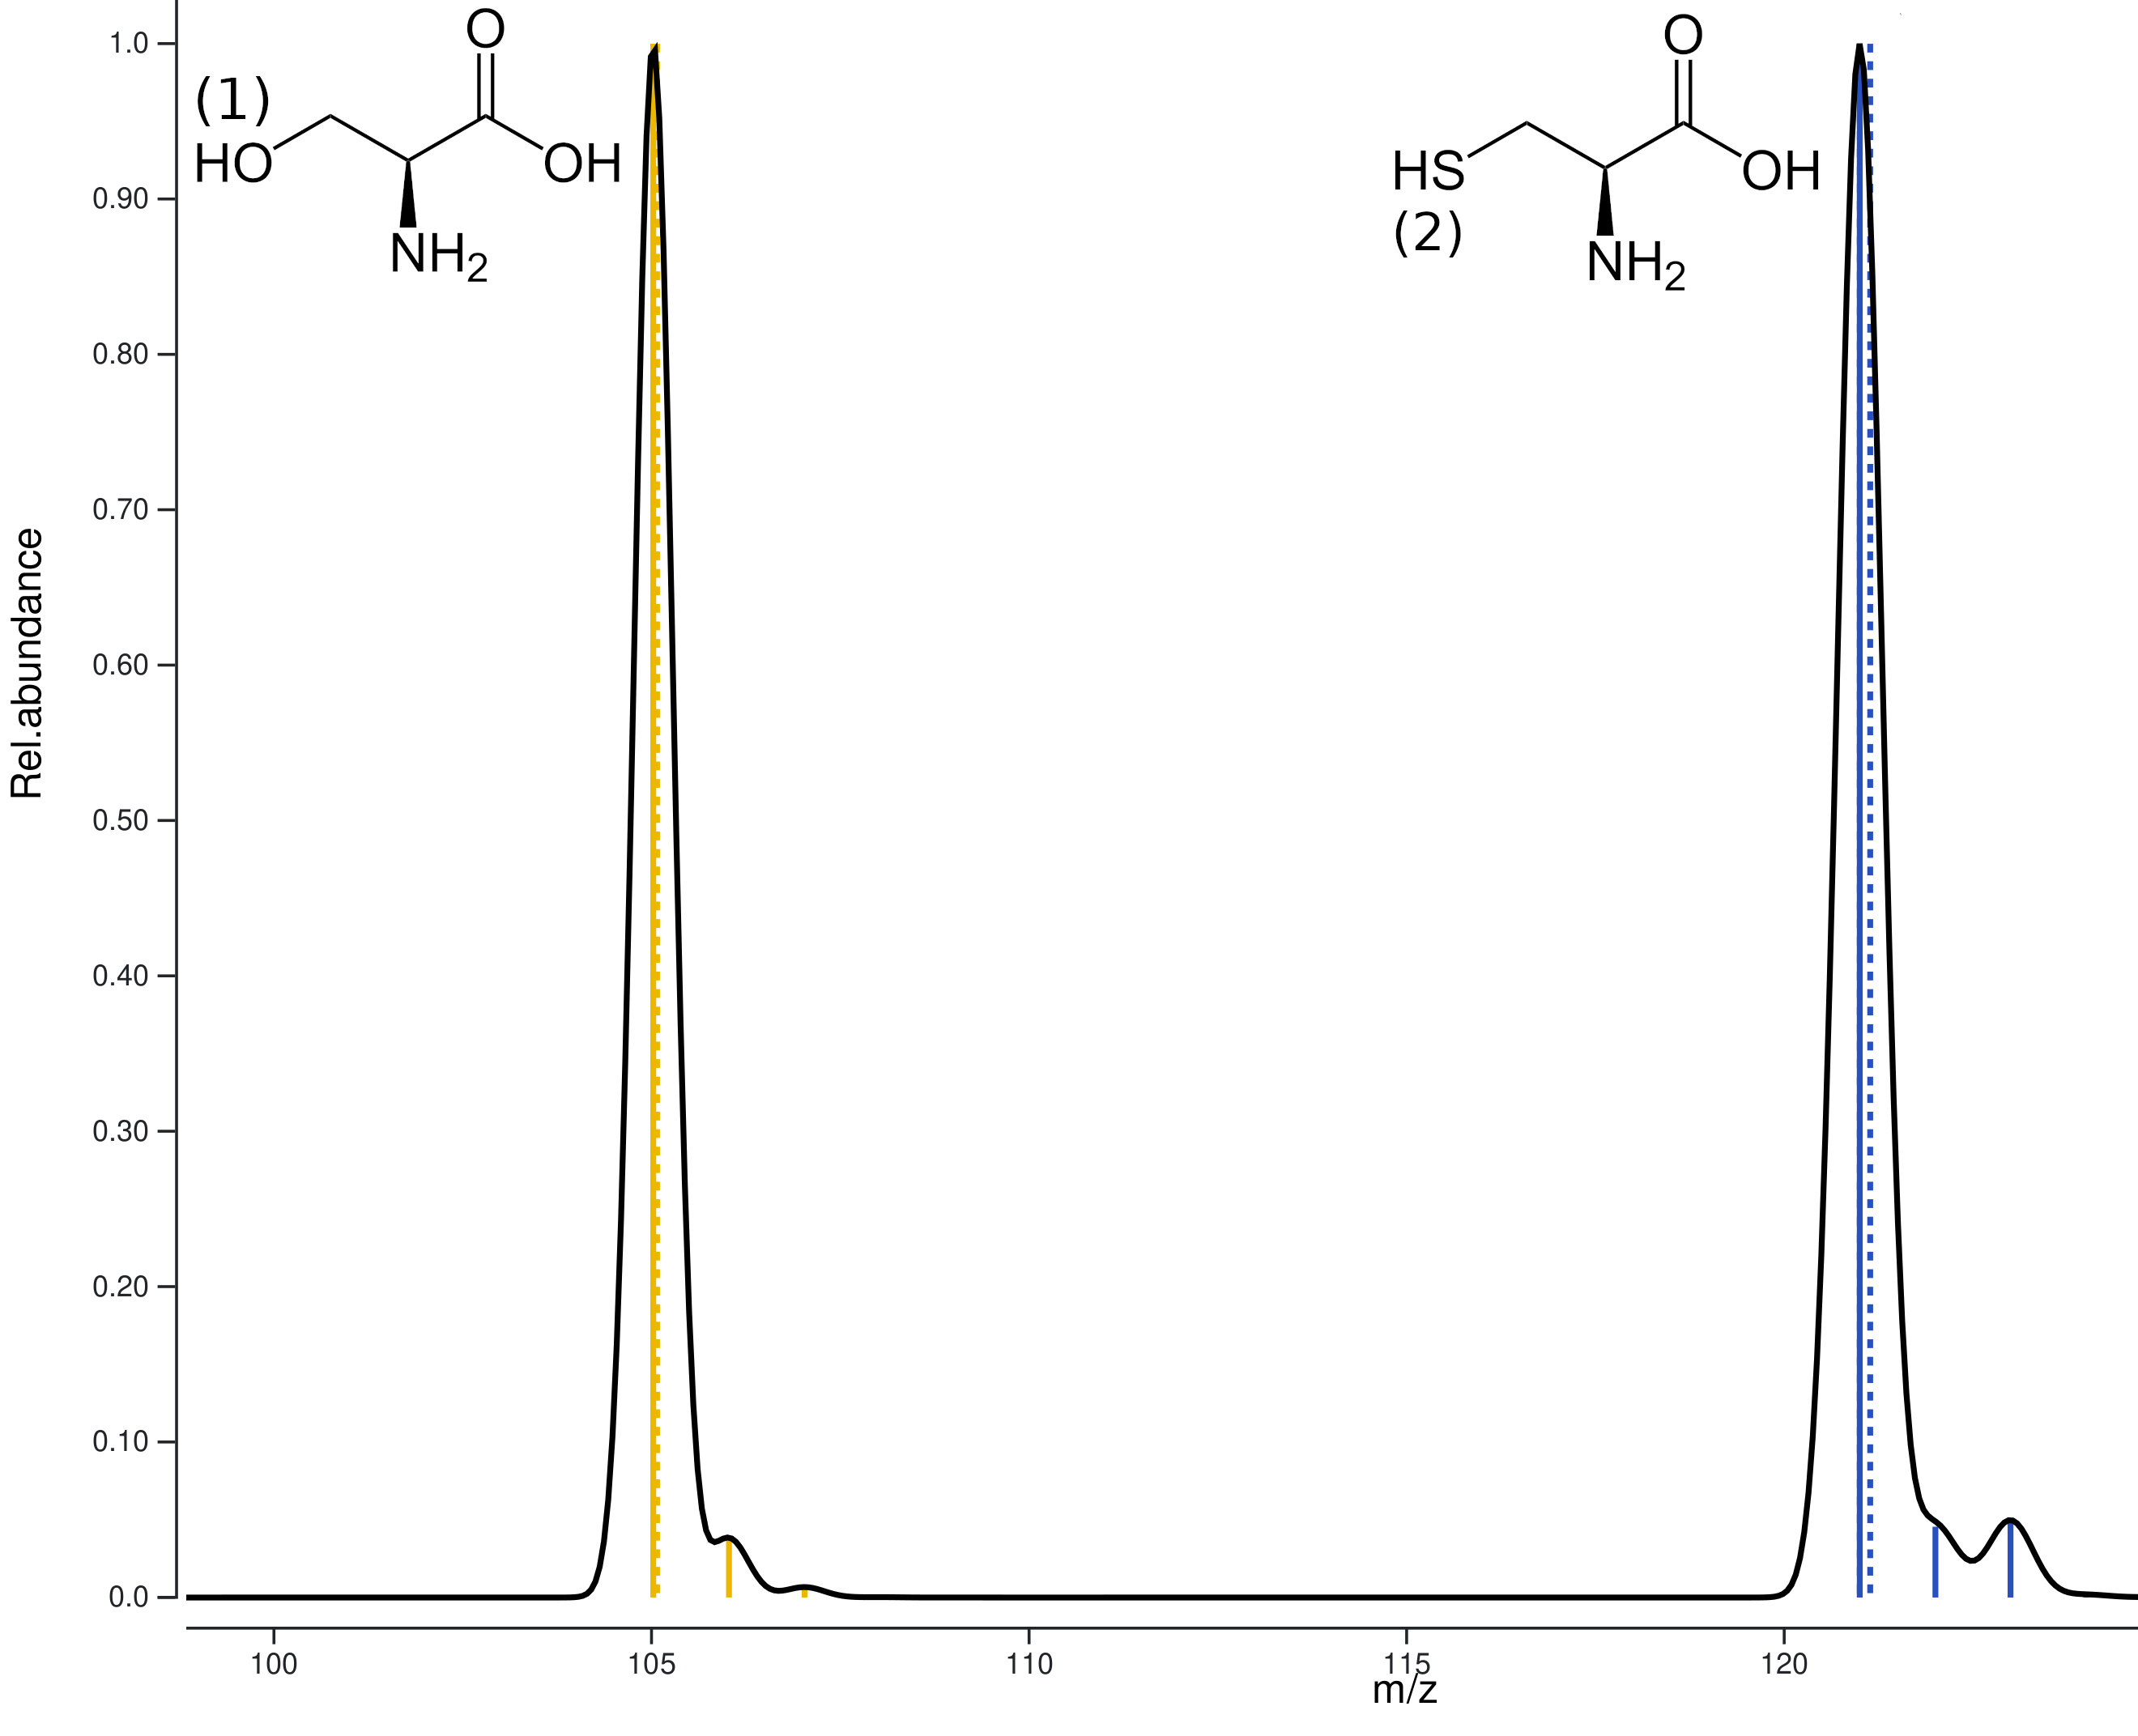
\includegraphics[width=0.75\textwidth]{./Resources/Simulated_Mass_Spectrum.png}
   \centering
   \caption{Computergeneriertes Massenspektrum von der Aminosäure \emph{Serin} (1) und \emph{Cystesin} (2). Peak von \emph{Serin} liegt bei 105; bei \emph{Systesin} um 121. y: relative Häufigkeit}
\end{figure}

Die Maxima werden \gerquot{Peaks} genannt und sind für eine Aminosäure an charakteristischer Position auf der $ x $-Achse. Obwohl sich die beiden Aminosäuren in der Abbildung \ref{fig:Sim_Mass_Spec} nur durch ein Atom unterscheiden (das linke Sauerstoffatom wurde durch ein Schwefelatom ersetzt) sind deren Massenspektren auf der $ x $-Achse weit voneinander entfernt und machen die beiden Aminosäuren dadurch sicher unterscheidbar.\\

Bei einzelnen Aminosäuren funktioniert die MS zuverlässig; bei Peptiden allerdings steht man vor dem Problem, dass das Massenspektrum unübersichtlicher wird und auch Peaks, die von Hintergrundrauschen stammen, schwerer herausgefiltert werden können. Abhilfe schafft hier die Tandem-Massenspektrometrie.

\subsection{Tandem-Massenspektrometrie (MS/MS)}\label{ss:Tandem_MS}
Bei der Tandem-Massenspektrometrie (MS/MS oder MS2) werden zwei MS Vorgänge hintereinander mit einer Probe durchgeführt. Die erste MS dient dazu Ionen aus einem bestimmten \massCharge Bereich auswählbar zu machen. Es entspricht also quasi einer Form der Filterung.

Vor der 2. MS werden die ausgewählten Reste einer Fragmentierung unterzogen. Bei einer Fragmentierung führt man Energie zu mit dem Ziel, dass die Ionen zerfallen und sog. Fragment-Ionen bilden. Diese Fragment-Ionen werden dann auf dem Massenspektrum nach der 2. MS sichtbar gemacht.

Fragment-Ionen sind kleiner als die ursprünglichen Ionen. So kann die 2. MS mit einer höheren Selektivität durchgeführt werden, welches Peaks durch Hintergrundrauschen verringert. Auch lassen sich Ionen besser identifizieren, die ein sehr ähnliches \massCharge-Verhältnis besitzen. Nach der 2. MS liegt eine Fülle an Fragment-Ionen-Peaks vor, aus denen sich die ursprünglichen Strukturinformationen ableiten lassen, da Ionen in spezifische Fragmente zerfallen \cite{Gross2013}. Zusammengefasst kann man sagen, dass das MS/MS Verfahren Ergebnisse höherer Güte erzeugt im Vergleich zur einfachen MS.

\section{De-Novo-Peptidsequenzierung mit \emph{pNovo+}}\label{s:pNovoPlusSeq}
Die \emph{pNovo+} Methode ist eine \gls{gls:DeNovo}, die mit einem \gls{gls:SpecGraph}en für die Auswertung der MS2-Spektren arbeitet und eine Erweiterung des \emph{pNovo} Verfahren darstellt \cite{pNovo}. Der Hauptansatz ist, dass zwei MS/MS Durchläufe mit jeweils verschiedenen Fragmentierungsmethoden\footnote{\emph{pNovo+} verwendet die higher energy
collisional dissociation (HCD) und die electron transfer dissociation (ETD) Fragmentierungsmethoden.} durchgeführt werden. Durch die Wahl einer anderen Fragmentierungsmethode ändert sich auch das MS2-Spektrum. Wenn nun Fragmentierungsmethoden verwendet werden, die möglichst komplementäre Spektren erzeugen, dann lässt sich durch das Zusammenführen der beiden MS2-Spektren die Qualität der Ergebnisse verbessern. Zum Beispiel lassen sich dadurch viele Peaks, die vom Hintergrundrauschen stammen, entfernen.

Für die Ermittlung der Sequenz eines Peptides wird zunächst ein Spektrums-Graph gebildet \dashAndSpace in Form eines DAG (directed acyclic graph). In diesem Graphen wird dann der längste Pfad bei gegebenen Start- und Endknoten berechnet. Die Reihenfolge der Knoten, die im längsten Pfad durchlaufen werden, stellt dann die Peptidsequenz dar.

\subsection{Vorverarbeitung der MS2-Spektren}\label{ss:Vorverarbeitung}
Bevor aus den MS2-Spektren der Spektrums-Graph gebildet werden kann, müssen die Daten vorverarbeitet werden. Für die Auswertung ist es von entscheidener Bedeutung, dass möglichst wenig Peaks verwendet werden, die vom Hintergrundrauschen stammen. Im weiteren Verlauf werden an einem exemplarischen MS2-Spektrum die Verarbeitungsschritte dargestellt.\\

Der erste Schritt ist das Verwenden des natürlichen Logarithmus der Intensitäten. Die Idee dabei ist, dass Hintergrundrauschen nicht überpriorisiert wird.

\begin{figure}[H]
   \centering
   \begin{minipage}[t]{.45\linewidth}
      \centering
      \begin{tikzpicture}[scale=\tikzScale, baseline=(current bounding box.center)]
         \draw [<->,thick] (0,\yAxisHeight) node (yaxis) [above] {\yAxisUnit}
         |- (\xAxisLength,0) node (xaxis) [right] {\xAxisUnit};
\draw[thick] (0.2, 0.0) -- (0.2, 2.3);
\draw[thick] (0.382, 0.0) -- (0.382, 1.7);
\draw[thick] (0.476, 0.0) -- (0.476, 2.7);
\draw[thick] (0.456, 0.0) -- (0.456, 1.8);
\draw[thick] (0.6859999999999999, 0.0) -- (0.6859999999999999, 2.7);
\draw[thick] (0.6839999999999999, 0.0) -- (0.6839999999999999, 1.8);
\draw[thick] (0.752, 0.0) -- (0.752, 1.1);
\draw[thick] (0.8200000000000001, 0.0) -- (0.8200000000000001, 2.2);
\draw[thick] (1.076, 0.0) -- (1.076, 1.5);
\draw[thick] (1.16, 0.0) -- (1.16, 1.9);
\draw[thick] (1.2120000000000002, 0.0) -- (1.2120000000000002, 2.0);
\draw[thick] (1.28, 0.0) -- (1.28, 1.9);
\draw[thick] (1.452, 0.0) -- (1.452, 1.3);
\draw[thick] (1.426, 0.0) -- (1.426, 1.9);
\draw[thick] (1.548, 0.0) -- (1.548, 1.9);
\draw[thick] (1.6740000000000002, 0.0) -- (1.6740000000000002, 1.5);
\draw[thick] (1.788, 0.0) -- (1.788, 2.5);
\draw[thick] (1.856, 0.0) -- (1.856, 2.3);
\draw[thick] (2.036, 0.0) -- (2.036, 1.7);
\draw[thick] (2.142, 0.0) -- (2.142, 1.6);
\draw[thick] (2.2520000000000002, 0.0) -- (2.2520000000000002, 2.0);
\draw[thick] (2.386, 0.0) -- (2.386, 1.6);
\draw[thick] (2.488, 0.0) -- (2.488, 2.9);
\draw[thick] (2.4739999999999998, 0.0) -- (2.4739999999999998, 2.7);
\draw[thick] (2.504, 0.0) -- (2.504, 2.0);
\draw[thick] (2.682, 0.0) -- (2.682, 2.0);
\draw[thick] (2.702, 0.0) -- (2.702, 2.5);
\draw[thick] (2.9259999999999997, 0.0) -- (2.9259999999999997, 2.8);
\draw[thick] (3.024, 0.0) -- (3.024, 2.4);
\draw[thick] (3.096, 0.0) -- (3.096, 1.8);
\draw[thick] (3.244, 0.0) -- (3.244, 2.6);
\draw[thick] (3.362, 0.0) -- (3.362, 1.9);
\draw[thick] (3.46, 0.0) -- (3.46, 2.3);
\draw[thick] (3.516, 0.0) -- (3.516, 1.1);
\draw[thick] (3.584, 0.0) -- (3.584, 1.8);
\draw[thick] (3.652, 0.0) -- (3.652, 2.0);
\draw[thick] (3.838, 0.0) -- (3.838, 1.5);
\draw[thick] (3.8819999999999997, 0.0) -- (3.8819999999999997, 2.6);
\draw[thick] (4.088, 0.0) -- (4.088, 2.6);
\draw[thick] (4.046, 0.0) -- (4.046, 1.1);
\draw[thick] (4.167999999999999, 0.0) -- (4.167999999999999, 2.0);
\draw[thick] (4.266, 0.0) -- (4.266, 2.4);
\draw[thick] (4.38, 0.0) -- (4.38, 1.1);
\draw[thick] (4.456, 0.0) -- (4.456, 2.2);
\draw[thick] (4.644, 0.0) -- (4.644, 2.6);
\draw[thick] (4.675999999999999, 0.0) -- (4.675999999999999, 2.5);
\draw[thick] (4.898000000000001, 0.0) -- (4.898000000000001, 1.2);
   \end{tikzpicture}%
   \end{minipage}%
   \textbf{$\rightarrow$} 
   \begin{minipage}[t]{.45\linewidth}
      \centering
      \begin{tikzpicture}[scale=\tikzScale, baseline=(current bounding box.center)]
      \draw [<->,thick] (0,\yAxisHeight) node (yaxis) [above] {\yAxisUnit}
      |- (\xAxisLength,0) node (xaxis) [right] {\xAxisUnit};
\draw[thick] (0.2, 0.0) -- (0.2, {ln(2.3)});
\draw[thick] (0.382, 0.0) -- (0.382, {ln(1.7)});
\draw[thick] (0.476, 0.0) -- (0.476, {ln(2.7)});
\draw[thick] (0.456, 0.0) -- (0.456, {ln(1.8)});
\draw[thick] (0.6859999999999999, 0.0) -- (0.6859999999999999, {ln(2.7)});
\draw[thick] (0.6839999999999999, 0.0) -- (0.6839999999999999, {ln(1.8)});
\draw[thick] (0.752, 0.0) -- (0.752, {ln(1.1)});
\draw[thick] (0.8200000000000001, 0.0) -- (0.8200000000000001, {ln(2.2)});
\draw[thick] (1.076, 0.0) -- (1.076, {ln(1.5)});
\draw[thick] (1.16, 0.0) -- (1.16, {ln(1.9)});
\draw[thick] (1.2120000000000002, 0.0) -- (1.2120000000000002, {ln(2.0)});
\draw[thick] (1.28, 0.0) -- (1.28, {ln(1.9)});
\draw[thick] (1.452, 0.0) -- (1.452, {ln(1.3)});
\draw[thick] (1.426, 0.0) -- (1.426, {ln(1.9)});
\draw[thick] (1.548, 0.0) -- (1.548, {ln(1.9)});
\draw[thick] (1.6740000000000002, 0.0) -- (1.6740000000000002, {ln(1.5)});
\draw[thick] (1.788, 0.0) -- (1.788, {ln(2.5)});
\draw[thick] (1.856, 0.0) -- (1.856, {ln(2.3)});
\draw[thick] (2.036, 0.0) -- (2.036, {ln(1.7)});
\draw[thick] (2.142, 0.0) -- (2.142, {ln(1.6)});
\draw[thick] (2.2520000000000002, 0.0) -- (2.2520000000000002, {ln(2.0)});
\draw[thick] (2.386, 0.0) -- (2.386, {ln(1.6)});
\draw[thick] (2.488, 0.0) -- (2.488, {ln(2.9)});
\draw[thick] (2.4739999999999998, 0.0) -- (2.4739999999999998, {ln(2.7)});
\draw[thick] (2.504, 0.0) -- (2.504, {ln(2.0)});
\draw[thick] (2.682, 0.0) -- (2.682, {ln(2.0)});
\draw[thick] (2.702, 0.0) -- (2.702, {ln(2.5)});
\draw[thick] (2.9259999999999997, 0.0) -- (2.9259999999999997, {ln(2.8)});
\draw[thick] (3.024, 0.0) -- (3.024, {ln(2.4)});
\draw[thick] (3.096, 0.0) -- (3.096, {ln(1.8)});
\draw[thick] (3.244, 0.0) -- (3.244, {ln(2.6)});
\draw[thick] (3.362, 0.0) -- (3.362, {ln(1.9)});
\draw[thick] (3.46, 0.0) -- (3.46, {ln(2.3)});
\draw[thick] (3.516, 0.0) -- (3.516, {ln(1.1)});
\draw[thick] (3.584, 0.0) -- (3.584, {ln(1.8)});
\draw[thick] (3.652, 0.0) -- (3.652, {ln(2.0)});
\draw[thick] (3.838, 0.0) -- (3.838, {ln(1.5)});
\draw[thick] (3.8819999999999997, 0.0) -- (3.8819999999999997, {ln(2.6)});
\draw[thick] (4.088, 0.0) -- (4.088, {ln(2.6)});
\draw[thick] (4.046, 0.0) -- (4.046, {ln(1.1)});
\draw[thick] (4.167999999999999, 0.0) -- (4.167999999999999, {ln(2.0)});
\draw[thick] (4.266, 0.0) -- (4.266, {ln(2.4)});
\draw[thick] (4.38, 0.0) -- (4.38, {ln(1.1)});
\draw[thick] (4.456, 0.0) -- (4.456, {ln(2.2)});
\draw[thick] (4.644, 0.0) -- (4.644, {ln(2.6)});
\draw[thick] (4.675999999999999, 0.0) -- (4.675999999999999, {ln(2.5)});
\draw[thick] (4.898000000000001, 0.0) -- (4.898000000000001, {ln(1.2)});
      \end{tikzpicture}
      \end{minipage}
      \caption{Anwendung des $ ln $ auf einem exemplarischen MS2-Spektrum.}
\end{figure}

Für das Verständnis des nächsten Schrittes muss man sich in Erinnerung rufen, dass eine gleiche Aminosäure keineswegs immer die gleiche Masse hat. Durch Isotope existiert eine gewisse \gerquot{Massenbandbreite} für ein und dieselbe Aminosäure. MS Systeme sind heute so genau, dass sie diese Differenzen erkennen. Dies hat den ungewollten Effekt, dass mehrere Peaks zu einer Aminosäure gehören können \cite{IsotopicDistributionMS}. Gleichzeitig können die \gerquot{Massenbandbreiten} zweier Aminosäuren sich überschneiden, sodass im ungünstigen Fall zwei Peaks kaum unterscheidbar nebeneinander liegen.\\

Eine Möglichkeit mit dieser Problematik umzugehen ist die Verwendung der monoisotopischen Masse. Die monoisotopische Masse ist die \gerquot{[...] exact mass of the most abundant naturally occurring stable isotope determined relative to the mass of 12 C, which is assigned the exact value of 12.0000.} \cite{MonoisotopicMass}. Ohne dabei jetzt tiefer ins Detail zu gehen kann man sagen, dass alle Peaks, deren Intensität mit einer möglichen monoisotopischen Masse übereinstimmen, auf jeden Fall einer Aminosäure entsprechen und (höchstwahrscheinlich)\footnote{Natürlich ist es möglich, dass das Rauschen zufällig einer monoisotopischen Masse entspricht. Die Wahrscheinlichkeit dafür ist allerdings sehr gering.} kein Hintergrundrauschen sind \cite{MassDefectMS}. Diese Peaks bekommen eine sogennante \emph{charge state}.\\

Der Algorithmus verwendet die \emph{charge state} Peaks als Ausganspunkte für weitere Berechnungen. Wenn die \massCharge Differenz zu einem anderen Peak einem Peptidfragment entspricht, dann stammt dieser Peak höchstwahrscheinlich von einem Fragment. Insgesamt werden damit die relevanten Peptidfragmente herausgeholt. Abbildung \ref{MonoisotopicMassFiltering} zeigt das Ergebnis nach den beiden zuvor genannten Schritten.

\begin{figure}[H]\label{MonoisotopicMassFiltering}
   \centering
   \begin{minipage}[t]{.45\linewidth}
      \centering
      \begin{tikzpicture}[scale=\tikzScale, baseline=(current bounding box.center)]
         \draw [<->,thick] (0,\yAxisHeight) node (yaxis) [above] {\yAxisUnit}
         |- (\xAxisLength,0) node (xaxis) [right] {\xAxisUnit};
\draw[thick] (0.2, 0.0) -- (0.2, {ln(2.3)});
\draw[color=blue!85!,opacity=.55,thick] (0.382, 0.0) -- (0.382, {ln(1.7)});
\draw[color=blue!85!,opacity=.55,thick] (0.476, 0.0) -- (0.476, {ln(2.7)});
\draw[color=magenta,thick] (0.456, 0.0) -- (0.456, {ln(1.8)});
\draw[color=blue!85!,opacity=.55,thick] (0.6859999999999999, 0.0) -- (0.6859999999999999, {ln(2.7)});
\draw[color=blue!85!,opacity=.55,thick] (0.6839999999999999, 0.0) -- (0.6839999999999999, {ln(1.8)});
\draw[thick] (0.752, 0.0) -- (0.752, {ln(1.1)});
\draw[thick] (0.8200000000000001, 0.0) -- (0.8200000000000001, {ln(2.2)});
\draw[thick] (1.076, 0.0) -- (1.076, {ln(1.5)});
\draw[thick] (1.16, 0.0) -- (1.16, {ln(1.9)});
\draw[thick] (1.2120000000000002, 0.0) -- (1.2120000000000002, {ln(2.0)});
\draw[thick] (1.28, 0.0) -- (1.28, {ln(1.9)});
\draw[color=blue!85!,opacity=.55,thick] (1.452, 0.0) -- (1.452, {ln(1.3)});
\draw[color=blue!85!,opacity=.55,thick] (1.426, 0.0) -- (1.426, {ln(1.9)});
\draw[color=magenta,thick] (1.548, 0.0) -- (1.548, {ln(1.9)});
\draw[color=blue!85!,opacity=.55,thick] (1.6740000000000002, 0.0) -- (1.6740000000000002, {ln(1.5)});
\draw[color=blue!85!,opacity=.55,thick] (1.788, 0.0) -- (1.788, {ln(2.5)});
\draw[thick] (1.856, 0.0) -- (1.856, {ln(2.3)});
\draw[thick] (2.036, 0.0) -- (2.036, {ln(1.7)});
\draw[thick] (2.142, 0.0) -- (2.142, {ln(1.6)});
\draw[thick] (2.2520000000000002, 0.0) -- (2.2520000000000002, {ln(2.0)});
\draw[thick] (2.386, 0.0) -- (2.386, {ln(1.6)});
\draw[color=blue!85!,opacity=.55,thick] (2.488, 0.0) -- (2.488, {ln(2.9)});
\draw[thick] (2.4739999999999998, 0.0) -- (2.4739999999999998, {ln(2.7)});
\draw[color=blue!85!,opacity=.55,thick] (2.504, 0.0) -- (2.504, {ln(2.0)});
\draw[color=magenta,thick] (2.682, 0.0) -- (2.682, {ln(2.0)});
\draw[color=blue!85!,opacity=.55,thick] (2.702, 0.0) -- (2.702, {ln(2.5)});
\draw[thick] (2.9259999999999997, 0.0) -- (2.9259999999999997, {ln(2.8)});
\draw[thick] (3.024, 0.0) -- (3.024, {ln(2.4)});
\draw[thick] (3.096, 0.0) -- (3.096, {ln(1.8)});
\draw[thick] (3.244, 0.0) -- (3.244, {ln(2.6)});
\draw[thick] (3.362, 0.0) -- (3.362, {ln(1.9)});
\draw[color=blue!85!,opacity=.55,thick] (3.46, 0.0) -- (3.46, {ln(2.3)});
\draw[color=blue!85!,opacity=.55,thick] (3.516, 0.0) -- (3.516, {ln(1.1)});
\draw[color=blue!85!,opacity=.55,thick] (3.584, 0.0) -- (3.584, {ln(1.8)});
\draw[color=magenta,thick] (3.652, 0.0) -- (3.652, {ln(2.0)});
\draw[color=blue!85!,opacity=.55,thick] (3.838, 0.0) -- (3.838, {ln(1.5)});
\draw[color=blue!85!,opacity=.55,thick] (3.8819999999999997, 0.0) -- (3.8819999999999997, {ln(2.6)});
\draw[thick] (4.088, 0.0) -- (4.088, {ln(2.6)});
\draw[thick] (4.046, 0.0) -- (4.046, {ln(1.1)});
\draw[thick] (4.167999999999999, 0.0) -- (4.167999999999999, {ln(2.0)});
\draw[thick] (4.266, 0.0) -- (4.266, {ln(2.4)});
\draw[color=blue!85!,opacity=.55,thick] (4.38, 0.0) -- (4.38, {ln(1.1)});
\draw[color=blue!85!,opacity=.55,thick] (4.456, 0.0) -- (4.456, {ln(2.2)});
\draw[color=magenta,thick] (4.644, 0.0) -- (4.644, {ln(2.6)});
\draw[color=blue!85!,opacity=.55,thick] (4.675999999999999, 0.0) -- (4.675999999999999, {ln(2.5)});
\draw[color=blue!85!,opacity=.55,thick] (4.898000000000001, 0.0) -- (4.898000000000001, {ln(1.2)});
   \end{tikzpicture}%
   \end{minipage}%
   \textbf{$\rightarrow$} 
   \begin{minipage}[t]{.45\linewidth}
      \centering
      \begin{tikzpicture}[scale=\tikzScale, baseline=(current bounding box.center)]
      \draw [<->,thick] (0,\yAxisHeight) node (yaxis) [above] {\yAxisUnit}
      |- (\xAxisLength,0) node (xaxis) [right] {\xAxisUnit};
\draw[color=blue!85!,opacity=.55,thick] (0.382, 0.0) -- (0.382, {ln(1.7)});
\draw[color=blue!85!,opacity=.55,thick] (0.476, 0.0) -- (0.476, {ln(2.7)});
\draw[color=magenta,thick] (0.456, 0.0) -- (0.456, {ln(1.8)});
\draw[color=blue!85!,opacity=.55,thick] (0.6859999999999999, 0.0) -- (0.6859999999999999, {ln(2.7)});
\draw[color=blue!85!,opacity=.55,thick] (0.6839999999999999, 0.0) -- (0.6839999999999999, {ln(1.8)});
\draw[color=blue!85!,opacity=.55,thick] (1.452, 0.0) -- (1.452, {ln(1.3)});
\draw[color=blue!85!,opacity=.55,thick] (1.426, 0.0) -- (1.426, {ln(1.9)});
\draw[color=magenta,thick] (1.548, 0.0) -- (1.548, {ln(1.9)});
\draw[color=blue!85!,opacity=.55,thick] (1.6740000000000002, 0.0) -- (1.6740000000000002, {ln(1.5)});
\draw[color=blue!85!,opacity=.55,thick] (1.788, 0.0) -- (1.788, {ln(2.5)});
\draw[color=blue!85!,opacity=.55,thick] (2.488, 0.0) -- (2.488, {ln(2.9)});
\draw[color=blue!85!,opacity=.55,thick] (2.504, 0.0) -- (2.504, {ln(2.0)});
\draw[color=magenta,thick] (2.682, 0.0) -- (2.682, {ln(2.0)});
\draw[color=blue!85!,opacity=.55,thick] (2.702, 0.0) -- (2.702, {ln(2.5)});
\draw[color=blue!85!,opacity=.55,thick] (3.46, 0.0) -- (3.46, {ln(2.3)});
\draw[color=blue!85!,opacity=.55,thick] (3.516, 0.0) -- (3.516, {ln(1.1)});
\draw[color=blue!85!,opacity=.55,thick] (3.584, 0.0) -- (3.584, {ln(1.8)});
\draw[color=magenta,thick] (3.652, 0.0) -- (3.652, {ln(2.0)});
\draw[color=blue!85!,opacity=.55,thick] (3.838, 0.0) -- (3.838, {ln(1.5)});
\draw[color=blue!85!,opacity=.55,thick] (3.8819999999999997, 0.0) -- (3.8819999999999997, {ln(2.6)});
\draw[color=blue!85!,opacity=.55,thick] (4.38, 0.0) -- (4.38, {ln(1.1)});
\draw[color=blue!85!,opacity=.55,thick] (4.456, 0.0) -- (4.456, {ln(2.2)});
\draw[color=magenta,thick] (4.644, 0.0) -- (4.644, {ln(2.6)});
\draw[color=blue!85!,opacity=.55,thick] (4.675999999999999, 0.0) -- (4.675999999999999, {ln(2.5)});
\draw[color=blue!85!,opacity=.55,thick] (4.898000000000001, 0.0) -- (4.898000000000001, {ln(1.2)});
      \end{tikzpicture}
      \end{minipage}
      \caption{Entfernen von Peaks, die keiner monoisotopischen Masse entsprechen oder benachbart mit einer Differenz von einem Fragment-Ion sind.}
\end{figure}

Tatsächlich ist die Verarbeitung an dieser Stelle noch etwas komplexer. So existieren auch noch sogenannte \emph{isotopic cluster}\footnote{Definition eines \emph{isotopic cluster} nach IUPAC: \gerquot{Group of peaks representing ions of the same elemental composition, but different isotopic compositions.} \cite[1556]{IUPACDefinitions}}, die gesondert verarbeitet werden. Für das grundsätzliche Prinzip ist dieses Detail allerdings weniger relevant.\\

Im letzten Vorberarbeitungsschritt werden Peaks aus einem irrelevanten \massCharge Bereich entfernt und naheliegende Peaks werden zusammengefasst, indem der Mittelwert sowol des \massCharge Wertes als auch der der Intensität besimmt wird. Üblicherweise liegt der Bereich für das Zusammenfassen bei $ +- 20 ppm $.

\begin{figure}[H]
   \centering
   \begin{minipage}[t]{.45\linewidth}
      \centering
      \begin{tikzpicture}[scale=\tikzScale, baseline=(current bounding box.center)]
         \draw [<->,thick] (0,\yAxisHeight) node (yaxis) [above] {\yAxisUnit}
         |- (\xAxisLength,0) node (xaxis) [right] {\xAxisUnit};
\draw[thick] (0.382, 0.0) -- (0.382, {ln(1.7)});
\draw[thick] (0.476, 0.0) -- (0.476, {ln(2.7)});
\draw[thick] (0.456, 0.0) -- (0.456, {ln(1.8)});
\draw[thick] (0.6859999999999999, 0.0) -- (0.6859999999999999, {ln(2.7)});
\draw[thick] (0.6839999999999999, 0.0) -- (0.6839999999999999, {ln(1.8)});
\draw[color=red,thick] (1.452, 0.0) -- (1.452, {ln(1.3)});
\draw[color=red,thick] (1.426, 0.0) -- (1.426, {ln(1.9)});
\draw[thick] (1.548, 0.0) -- (1.548, {ln(1.9)});
\draw[thick] (1.6740000000000002, 0.0) -- (1.6740000000000002, {ln(1.5)});
\draw[thick] (1.788, 0.0) -- (1.788, {ln(2.5)});
\draw[color=red,thick] (2.488, 0.0) -- (2.488, {ln(2.9)});
\draw[color=red,thick] (2.504, 0.0) -- (2.504, {ln(2.0)});
\draw[color=red,thick] (2.682, 0.0) -- (2.682, {ln(2.0)});
\draw[color=red,thick] (2.702, 0.0) -- (2.702, {ln(2.5)});
\draw[thick] (3.46, 0.0) -- (3.46, {ln(2.3)});
\draw[thick] (3.516, 0.0) -- (3.516, {ln(1.1)});
\draw[thick] (3.584, 0.0) -- (3.584, {ln(1.8)});
\draw[thick] (3.652, 0.0) -- (3.652, {ln(2.0)});
\draw[color=red,thick] (3.838, 0.0) -- (3.838, {ln(1.5)});
\draw[color=red,thick] (3.8819999999999997, 0.0) -- (3.8819999999999997, {ln(2.6)});
\draw[thick] (4.38, 0.0) -- (4.38, {ln(1.1)});
\draw[thick] (4.456, 0.0) -- (4.456, {ln(2.2)});
\draw[thick] (4.644, 0.0) -- (4.644, {ln(2.6)});
\draw[thick] (4.675999999999999, 0.0) -- (4.675999999999999, {ln(2.5)});
\draw[thick] (4.898000000000001, 0.0) -- (4.898000000000001, {ln(1.2)});

\fill[red!25!,opacity=.25] (0,0) rectangle (1,\yAxisHeight-\axisColorOffset);
         \fill[red!25!,opacity=.25] (\xAxisLength-1,0) rectangle (\xAxisLength-\axisColorOffset,\yAxisHeight-\axisColorOffset);
         \fill[green!25!,opacity=.25] (1,0) rectangle (\xAxisLength-1,\yAxisHeight-\axisColorOffset);
   \end{tikzpicture}%
   \end{minipage}%
   \textbf{$\rightarrow$} 
   \begin{minipage}[t]{.45\linewidth}
      \centering
      \begin{tikzpicture}[scale=\tikzScale, baseline=(current bounding box.center)]
      \draw [<->,thick] (0,\yAxisHeight) node (yaxis) [above] {\yAxisUnit}
      |- (\xAxisLength,0) node (xaxis) [right] {\xAxisUnit};
%\draw[color=red,thick] (1.452, 0.0) -- (1.452, {ln(1.3)});
%\draw[color=red,thick] (1.426, 0.0) -- (1.426, {ln(1.9)});
\draw[color=red,ultra thick] ({(1.452+1.426)/2}, 0.0) -- ({(1.452+1.426)/2}, {(ln(1.3)+ln(1.9))/2});

\draw[thick] (1.548, 0.0) -- (1.548, {ln(1.9)});
\draw[thick] (1.6740000000000002, 0.0) -- (1.6740000000000002, {ln(1.5)});
\draw[thick] (1.788, 0.0) -- (1.788, {ln(2.5)});

%\draw[color=red,thick] (2.488, 0.0) -- (2.488, {ln(2.9)});
%\draw[color=red,thick] (2.504, 0.0) -- (2.504, {ln(2.0)});
\draw[color=red,ultra thick] ({(2.488+2.504)/2}, 0.0) -- ({(2.488+2.504)/2}, {(ln(2.9)+ln(2.0))/2});

%\draw[color=red,thick] (2.682, 0.0) -- (2.682, {ln(2.0)});
%\draw[color=red,thick] (2.702, 0.0) -- (2.702, {ln(2.5)});
\draw[color=red,ultra thick] ({(2.682+2.702)/2}, 0.0) -- ({(2.682+2.702)/2}, {(ln(2.0+ln(2.5))/2});

\draw[thick] (3.46, 0.0) -- (3.46, {ln(2.3)});
\draw[thick] (3.516, 0.0) -- (3.516, {ln(1.1)});
\draw[thick] (3.584, 0.0) -- (3.584, {ln(1.8)});
\draw[thick] (3.652, 0.0) -- (3.652, {ln(2.0)});

%\draw[color=red,thick] (3.838, 0.0) -- (3.838, {ln(1.5)});
%\draw[color=red,thick] (3.8819999999999997, 0.0) -- (3.8819999999999997,{ln(2.6)});
\draw[color=red,ultra thick] ({(3.838+3.8819999999999997)/2}, 0.0) -- ({(3.838+3.8819999999999997)/2}, {(ln(1.5)+ln(2.6))/2});

\fill[red!25!,opacity=.25] (0,0) rectangle (1,\yAxisHeight-\axisColorOffset);
         \fill[red!25!,opacity=.25] (\xAxisLength-1,0) rectangle (\xAxisLength-\axisColorOffset,\yAxisHeight-\axisColorOffset);
         \fill[green!25!,opacity=.25] (1,0) rectangle (\xAxisLength-1,\yAxisHeight-\axisColorOffset);
      \end{tikzpicture}
      \end{minipage}
      \caption{Entfernen von Peaks aus einem irrelevanten \massCharge Bereich und zusammenfassen naheliegender Peaks. Rot markierte Peaks sind jene, die zusammengefasst werden.}
\end{figure}

\subsection{Bildung eines Spektrums-Graphen}\label{ss:BildungSpekGraph}
Der Spektrums-Graph wird aus einem vorverarbeiteten MS2-Spektrum (siehe Kapitel: \ref{ss:Vorverarbeitung}) gebildet. Im initialen Zustand werden die Peaks als Knoten interpretiert. Dazu kommt ein Start- und Endknoten. Jedem Knoten wird eine Masse zugeordet; im initialen Zustand bekommt der Startknoten die Masse 0 und der Endknoten die Masse des vorherigen Knotens minus der Masse des Wassers ($ 18,02 $). Die Masse der übrigen Knoten entsprechen ihren jeweils korrespondierenden \massCharge Wert. Die gerichteten Kanten werden zwischen einem Knotenpaar hinzugefügt, wenn die Differenz deren Masse gleich ist mit der Masse von ein oder zwei Aminosäuren.

\subsection{Identifikation der Aminosäuresequenz}
Der gebildete DAG kann mit klassischen Algorithmen, die den längsten Pfad suchen, durchlaufen werden. Bezogen auf die Graphentheorie entspricht die Ermittlung der Aminosäurensequenz dem Suchen eines bestimmten Pfades \dashAndSpace und nicht nach irgendeinem Pfad. Daher muss der Algorithmus mittels einer Breitensuche arbeiten, um alle möglichen Pfade zu bestimmen.

In aller Regel wird es mehrere Pfade geben. Bestimmte Sequenzen sind wahrscheinlicher als andere. So sind Pfade mit Kanten, die wegen der Massendifferenz von genau einer Aminosäure gebildet wurden, wahrscheinlicher \cite{pNovoPlus}. Alle Pfade bekommen mittels einer Scoring-Funktion einen Wert zugewiesen. Der Pfad mit dem höchsten Scoring-Wert ist wahrscheinlich das richtige Ergebnis. Die Scoring-Funktion berücksichtigt unter anderem wie viele Fragmente, die einer bestimmten Aminosäure zugeordet werden können, im MS2-Spektrum vorhanden sind \cite{pNovo}. Die Sequenz mit dem höchsten Scoring-Wert ist das Endergebnis.

\section{De-Novo-Peptidsequenzierung mit \emph{Open-pNovo}}\label{s:OpenpNovoSeq}
Bei Proteinen können posttranslationale Proteinmodifikationen (PTM) auftreten. PTMs sind Ereignisse, bei denen sich Änderungen im Protein einstellen \cite{Mann2003}; teilweise sind die Änderungen von einer Zelle erwünscht \dashAndSpace teilweise stammen sie aber auch zum Beispiel von unerwünschten Wechselwirkungen nebeneinanderliegenden Aminosäuren. Ein Teil dieser PTMs führen zu einer Änderung der Aminosäuresequenz. Dies ist für die \gls{gls:DeNovo} nicht weiter problematisch, da sowieso ohne eine Datenbank gearbeitet wird, sodass solche PTMs nicht einmal auffallen würden. Andere PTMs hingegen haben die Auswirkung, dass Stoffe gebildet werden, die nicht mehr zu der Gruppe der proteinogenen Aminosäuren gehören. Proteinogene Aminosäuren sind jene Aminosäuren, die für den Bau von Proteinen verwendet werden. Der Effekt ist also, dass Stoffe (oder deren Fragmente) bei einem Massenspektrum angezeigt werden, die kein Teil eines Peptids sein können. Bei der Sequenzierung von Peptidfragmenten muss dies daher berücksichtigt werden.
Wenn im weiteren Verlauf von PTMs gesprochen wird, dann sind solche gemeint, die für die \gls{gls:DeNovo} relevant sind.

Open-pNovo ist ein \gls{gls:DeNovo}sverfahren, welches auf pNovo+ Tool aufbaut und versucht die Problematik mit den PTMs zu lösen.

\subsection{PTMs im konstruierten DAG}
Die Konvertierung eines MS2-Spektrums läuft bis zum DAG analog ab wie in den Kapiteln \ref{ss:Vorverarbeitung} und \ref{ss:BildungSpekGraph} für pNovo+. Der Unterschied ist nun, dass es zwei Arten von Kanten gibt:

\begin{itemize}
   \item \gerquot{Normale} Kanten: Kanten, die gebildet werden, wie es bereits für \emph{pNovo+} gezeigt wurde. 
   \item \gerquot{Modifizierte} Kanten: Kanten, die zum Grahpen hinzugefügt werden, wenn die Massendifferenz zweier Knoten der Masse einer Aminosäure plus der Masse einer möglichen PTM-Änderung entspricht. 
\end{itemize}

Eine Liste aller PTMs in der Datenbank Unimod (sowohl relevante als auch nicht relevante) beinhaltet aktuell 1510 Einträge\footnote{Siehe: \url{https://www.ebi.ac.uk/ols/ontologies/unimod}} (Stand: 18.04.2022). Für die modifizierten Kanten gibt es insgesamt $ 1510 * 20 = 30200 $ mögliche Differenzen, wobei viele davon nicht relevante PTMs sind. Zum Vergleich: bei den normalen Kanten gibt es $ 20^2 = 400 $ mögliche Differenzen.

Die hohe Anzahl an Differenzen für modifizierte Kanten hat die Konsequenz, dass viele Knoten zufällig verbunden werden und dass dadurch die Genauigkeit der Ergebnisse abnimmt. Dieses Problem kann man durch eine geringere Liste an möglichen PTMs abfedern, allerdings mit einem Verlust  der Genauigkeit auf Seiten der PTMs. Es ist hier also eine Abwägung.

\subsection{Evaluierung von Open-pNovo}
Open-pNovo wurde sowohl auf drei realen als auch auf drei generierten Testdaten getestet. Tabelle \ref{tab:OpenPNovoResults} zeigt die Ergebnisse im Vergleich zu pNovo+ und zwei anderen Algorithmen. Die Datensätze enthielten die am häufigsten vorkommenden PTMs.

\begin{table}[H]
    \centering
    \begin{tabular}{l|c|c|c|c}
        \toprule
        \textbf{Testdatensätze} & \textbf{Open-pNovo+} & \textbf{pNovo+} & \textbf{PEAKS} & \textbf{Novor} \\
        \midrule
        Real (20259) & $76,3 \%$ & $68,5 \%$ & $65,8 \%$ & $39,9 \%$ \\
        Generiert (17877) & $77,8 \%$ & $0,6 \%$ & $0,5 \%$ & $0,2 \%$ \\
        \bottomrule
    \end{tabular}
    \newline
    \caption{Vergleich der durchschnittlichen richtigen \gls{gls:DeNovo} Peptidsequenzierungen von Open-pNovo und anderen Algorithmen \cite[650]{OpenPNovo}.}
    \label{tab:OpenPNovoResults}
\end{table}

Die enorm schlechten Ergebnisse der anderen Algorithmen bei den generierten Testdaten ist ein Nebeneffekt des Ziels bei der Testdatengenerierung. Denn diese wurden so ausgelegt, um die Grenzen von Open-pNovo+ zu ermitteln \cite[649]{OpenPNovo}. Eine Aussagekraft haben diese Ergebnisse also nicht. Allerdings auch bei realen Testdaten zeigt sich Open-pNovo als voll konkurrenzfähig gegenüber den anderen Algorithmen.

Noch besser zeigt sich Open-pNovo, wenn der Recall Wert betrachtet wird \dashAndSpace also die Anzahl an verschiedenen PSMs, die erkannt wurden. In diesem Fall ist der Abstand zu den anderen Algorithmen deutlich größer geworden.

\begin{table}[H]
    \centering
    \begin{tabular}{l|c|c|c|c}
        \toprule
        \textbf{Testdatensätze} & \textbf{Open-pNovo+} & \textbf{pNovo+} & \textbf{PEAKS} & \textbf{Novor} \\
        \midrule
        Real (5034) & $61,6 \%$ & $31,3 \%$ & $32,0 \%$ & $13,7 \%$ \\
        \bottomrule
    \end{tabular}
    \newline
    \caption{Vergleich der durchschnittlichen Recall Werte einer \gls{gls:DeNovo} Peptidsequenzierungen von Open-pNovo und anderen Algorithmen \cite[650]{OpenPNovo}.}
    \label{tab:OpenPNovoResultsRecall}
\end{table}

\subsection{Zusammenfassung}


% Die \gls{gls:DeNovo} nutzt die sogenannte \gls{gls:TMassSpek} für die Bestimmung der Peptidsequenz. Dabei wird die physikalische Eigenschaft ausgenutzt, dass jedes Atom bzw. jedes Molekül \dashAndSpace wenn es einer \gls{gls:Ionisation} unterzogen wurde \dashAndSpace ein charakteristisches \gls{gls:MassSpek} besitzt. Das \gls{gls:MassSpek} stellt also eine Art \gerquot{Fingerabdruck} eines Moleküls dar und macht dieses ermittelbar.

% U.U. eine Beispielgrafik eines Massenspektrums hinzufuegen ...

\subsubsection{\glsentrytext{gls:TMassSpek} bei größeren Molekülen}
Bei größeren Molekülen (wie einem Protein) führt die \gls{gls:Ionisation} dazu, dass das Molekül in kleinere spezifische Ionen zerfällt (sog. Fragmentierung). Die Fragmentierungsinformationen einer \gls{gls:DeNovo} sind meist unvollständig, da fehlende Daten bei einem Fragmentierungsschritt die Güte des Endergebnisses negativ beeinflusst. Dies wird insbesondere dann ein Problem, wenn unbekannte Änderungen in einer Peptidsequenz vorhanden sind.

Um dieses Problem zu verringern können unterschiedliche Techniken parallel eingesetzt werden, welche verschiedene Fragmente erzeugen und daher auch verschiedenartige \glspl{gls:MassSpek} zur Folge haben.\footnote{Konkret: Es wird sowohl das \gls{acr:HCD} als auch das \gls{acr:ETD} Verfahren angewendet.}

\subsection{Datenaufbereitung}
Typischerweise betrachtet man die sog. \gerquot{\glspl{gls:Peak}} in den \glspl{gls:MassSpek}. Jeder \gls{gls:Peak} stellt ein unterschiedliches Ion dar. Dazu kommen Messungenauigkeiten sowie Hintergrundrauschen. Durch die hohe Anzahl an möglichen Ionen kann nicht ohne weiteres differenziert werden, welcher der \glspl{gls:Peak} von welchen Ionen erzeugt wurden und welche nicht.

% Frage an Dominik: Ist hier eine einfache Auflistung an Techniken für die Datenaufbereitung besser?
Der Algorithmus für die Datenaufbereitung berechnet den natürlichen Logarithmus von den Intensitäten der \glspl{gls:Peak}, um Hintergrundrauschen und Messungenauigkeiten nicht überzupriorisieren. Zusätzlich dazu werden \glspl{gls:Peak}, die in einem Toleranzbereich nebeneinander liegen, zusammengefasst. Am Ende werden die \glspl{gls:Peak} entfernt, bei denen bekannt ist, dass es sich nicht um relevante Ionen handeln kann. (z.B. \glspl{gls:Peak} von Isotopen)

\begin{figure}[H]
   \centering
   \begin{minipage}[t]{.4\linewidth}
      \centering
      \begin{tikzpicture}[scale=\tikzScale, baseline=(current bounding box.center)]
         \draw [<->,thick] (0,2.75) node (yaxis) [above] {\yAxisUnit}
         |- (3,0) node (xaxis) [right] {\xAxisUnit};

         \draw[thick] (0.2,0) -- (0.2,1.1);
         \draw[thick] (0.3,0) -- (0.3,1.6);
         \draw[thick] (0.6,0) -- (0.6,1.7);
         \draw[thick] (0.8,0) -- (0.8,1.2);
         \draw[thick] (1.0,0) -- (1.0,1.1);

         \draw[color=red,thick] (1.2,0) -- (1.2,2.65);
         \draw[thick] (1.4,0) -- (1.4,1.4);
         \draw[thick] (1.6,0) -- (1.6,1.2);
         \draw[thick] (1.8,0) -- (1.8,1.3);
         \draw[thick] (2.0,0) -- (2.0,1.8);

         \draw[thick] (1.1,0) -- (1.1,2.0);
         \draw[color=red,thick] (0.35,0) -- (0.35,2.25);
         \draw[thick] (1.9,0) -- (1.9,1.4);
         \draw[color=red,thick] (2.2,0) -- (2.2,2.6);
         \draw[thick] (2.5,0) -- (2.5,1.25);

         \draw[thick] (2.7,0) -- (2.7,1.1);
         \foreach \x in {1,...,6}
         {
            \draw[thick] (1.2+\x*0.05,0) -- (1.2+\x*0.05,1.0+\x*0.15);
         }
      \end{tikzpicture}%
      % \subcaption{Exemplarische Rohdaten}
   \end{minipage}%
   \textbf{$\rightarrow$}
   \begin{minipage}[t]{.4\linewidth}
      \centering
      \begin{tikzpicture}[scale=\tikzScale, baseline=(current bounding box.center)]
         \draw [<->,thick] (0,2.75) node (yaxis) [above] {\yAxisUnit}
         |- (3,0) node (xaxis) [right] {\xAxisUnit};

         \draw[thick] (0.2,0) -- (0.2,{ln(1.1)});
         \draw[thick] (0.3,0) -- (0.3,{ln(1.6)});
         \draw[thick] (0.6,0) -- (0.6,{ln(1.7)});
         \draw[thick] (0.8,0) -- (0.8,{ln(1.2)});
         \draw[thick] (1.0,0) -- (1.0,{ln(1.1)});

         \draw[color=red,thick] (1.2,0) -- (1.2,{ln(2.65)});
         \draw[thick] (1.4,0) -- (1.4,{ln(1.4)});
         \draw[thick] (1.6,0) -- (1.6,{ln(1.2)});
         \draw[thick] (1.8,0) -- (1.8,{ln(1.3)});
         \draw[thick] (2.0,0) -- (2.0,{ln(1.8)});

         \draw[thick] (1.1,0) -- (1.1,{ln(2.0)});
         \draw[color=red,thick] (0.35,0) -- (0.35,{ln(2.25)});
         \draw[thick] (1.9,0) -- (1.9,{ln(1.4)});
         \draw[color=red,thick] (2.2,0) -- (2.2,{ln(2.6)});
         \draw[thick] (2.5,0) -- (2.5,{ln(1.25)});

         \draw[thick] (2.7,0) -- (2.7,{ln(1.1)});
         \foreach \x in {1,...,6}
         {%
            \draw[thick] (1.2+\x*0.05,0) -- (1.2+\x*0.05,{ln(1.0+\x*0.15)});
         }
      \end{tikzpicture}
      %\subcaption{Exemplarische Rohdaten}
   \end{minipage}
   \caption{Anwendung des $ln$ auf Rohdaten. Rote \glspl{gls:Peak} stellen hier exemplarisch fehlerhafte Daten dar, die nach dem $ln$ reduziert wurden.}
\end{figure}

\begin{figure}[H]
   \centering
   \begin{minipage}[t]{.4\linewidth}
      \centering
      \begin{tikzpicture}[scale=\tikzScale, baseline=(current bounding box.center)]
         \draw [<->,thick] (0,2.75) node (yaxis) [above] {\yAxisUnit}
         |- (3,0) node (xaxis) [right] {\xAxisUnit};

         \draw[thick] (0.2,0) -- (0.2,{ln(1.1)});
         \draw[thick] (0.3,0) -- (0.3,{ln(1.6)});
         \draw[thick] (0.6,0) -- (0.6,{ln(1.7)});
         \draw[thick] (0.8,0) -- (0.8,{ln(1.2)});
         \draw[thick] (1.0,0) -- (1.0,{ln(1.1)});

         \draw[thick] (1.2,0) -- (1.2,{ln(2.65)});
         \draw[thick] (1.4,0) -- (1.4,{ln(1.4)});
         \draw[thick] (1.6,0) -- (1.6,{ln(1.2)});
         \draw[thick] (1.8,0) -- (1.8,{ln(1.3)});
         \draw[thick] (2.0,0) -- (2.0,{ln(1.8)});

         \draw[thick] (1.1,0) -- (1.1,{ln(2.0)});
         \draw[thick] (0.35,0) -- (0.35,{ln(2.25)});
         \draw[thick] (1.9,0) -- (1.9,{ln(1.4)});
         \draw[thick] (2.2,0) -- (2.2,{ln(2.6)});
         \draw[thick] (2.5,0) -- (2.5,{ln(1.25)});

         \draw[thick] (2.7,0) -- (2.7,{ln(1.1)});
         \foreach \x in {1,...,6}
         {%
            \draw[color=red,thick] (1.2+\x*0.05,0) -- (1.2+\x*0.05,{ln(1.0+\x*0.15)});
         }

         \draw[dotted] (0.4,0) -- (0.4,2.75);
         \draw[dotted] (2.6,0) -- (2.6,2.75);
         \fill[red!25!,opacity=.25] (0,0) rectangle (0.4,2.75);
         \fill[red!25!,opacity=.25] (2.6,0) rectangle (3.0,2.75);
         \fill[green!25!,opacity=.25] (0.4,0) rectangle (2.6,2.75);
      \end{tikzpicture}
      %\subcaption{Exemplarische Rohdaten}
   \end{minipage}
   \textbf{$\rightarrow$}
   \begin{minipage}[t]{.4\linewidth}
      \centering
      \begin{tikzpicture}[scale=\tikzScale, baseline=(current bounding box.center)]
         \draw [<->,thick] (0,2.75) node (yaxis) [above] {\yAxisUnit}
         |- (3,0) node (xaxis) [right] {\xAxisUnit};

         \draw[thick] (0.6,0) -- (0.6,{ln(1.7)});
         \draw[thick] (0.8,0) -- (0.8,{ln(1.2)});
         \draw[thick] (1.0,0) -- (1.0,{ln(1.1)});

         \draw[thick] (1.2,0) -- (1.2,{ln(2.65)});
         %\draw[thick] (1.4,0) -- (1.4,{ln(1.4)});
         \draw[thick] (1.6,0) -- (1.6,{ln(1.2)});
         \draw[thick] (1.8,0) -- (1.8,{ln(1.3)});
         \draw[thick] (2.0,0) -- (2.0,{ln(1.8)});

         \draw[thick] (1.1,0) -- (1.1,{ln(2.0)});
         \draw[thick] (1.9,0) -- (1.9,{ln(1.4)});
         \draw[thick] (2.2,0) -- (2.2,{ln(2.6)});
         \draw[thick] (2.5,0) -- (2.5,{ln(1.25)});

         \draw[color=red,ultra thick] (1.2+1*0.05,0) -- (1.2+1*0.05,{ln(1.0+1*0.15)});
         \draw[color=red,ultra thick] (1.2+3*0.05,0) -- (1.2+3*0.05,{ln(1.0+3*0.15)});
         \draw[color=red,ultra thick] (1.2+5*0.05,0) -- (1.2+5*0.05,{ln(1.0+5*0.15)});

         \draw[dotted] (0.4,0) -- (0.4,2.75);
         \draw[dotted] (2.6,0) -- (2.6,2.75);
         \fill[red!25!,opacity=.25] (0,0) rectangle (0.4,2.75);
         \fill[red!25!,opacity=.25] (2.6,0) rectangle (3.0,2.75);
         \fill[green!25!,opacity=.25] (0.4,0) rectangle (2.6,2.75);
      \end{tikzpicture}
      %\subcaption{Exemplarische Rohdaten}
   \end{minipage}
   \caption{Entfernen von irrelevanten \glspl{gls:Peak} sowie zusammenfassen naheliegender \glspl{gls:Peak}. Hier symbolisieren die roten \glspl{gls:Peak} jene, die zusammengefasst werden.}
\end{figure}

% `\glsentrytext` funktioniert nicht für `\glspl`
\subsection{Konvertierung von \glspl{gls:MassSpek}}
Das Ziel der Konvertierung ist das Erzeugen eines \gls{gls:SpecGraph}en. Um von einem \gls{gls:MassSpek} zu einem \gls{gls:SpecGraph}en zu kommen, werden die \glspl{gls:Peak}, die nach der Datenaufbereitung (Siehe ...) übrig bleiben, als Knoten gewertet. Dazu kommt ein Start- und Endknoten. Jeder Knoten bekommt eine Gewichtung; diese Gewichtung entspricht der Stärke des \gls{gls:Peak}s.

\newcommand{\colorA}{white!30!green}
\newcommand{\colorB}{black!10!yellow}
\newcommand{\colorC}{white!40!red}
\newcommand{\colorD}{white!25!orange}
\newcommand{\colorE}{white!45!blue}
\newcommand{\colorF}{white!5!magenta}
\newcommand{\nodeFontSize}{\scriptsize}
\newcommand{\nodeScaleFactor}{100}
\newcommand{\round}[1]{\pgfmathprintnumber[precision=0]{#1}}
\newcommand{\rawA}{ln(1.7)}
\newcommand{\rawB}{ln(2.0)}
\newcommand{\rawC}{ln(2.65)}
\newcommand{\rawD}{ln(1.0+5*0.15)}
\newcommand{\rawE}{ln(1.85)}
\newcommand{\rawF}{ln(2.6)}
\newcommand{\valueA}{\pgfmathparse{int(\rawA*\nodeScaleFactor)}\pgfmathresult}
\newcommand{\valueB}{\pgfmathparse{int(\rawB*\nodeScaleFactor)}\pgfmathresult}
\newcommand{\valueC}{\pgfmathparse{int(\rawC*\nodeScaleFactor)}\pgfmathresult}
\newcommand{\valueD}{\pgfmathparse{int(\rawD*\nodeScaleFactor)}\pgfmathresult}
\newcommand{\valueE}{\pgfmathparse{int(\rawE*\nodeScaleFactor)}\pgfmathresult}
\newcommand{\valueF}{\pgfmathparse{int(\rawF*\nodeScaleFactor)}\pgfmathresult}

\begin{figure}[htb]
   \centering
      \begin{tikzpicture}[scale=\tikzScale*1.5, baseline=(current bounding box.center)]
         \draw [<->,thick] (0,2.75) node (yaxis) [above] {\yAxisUnit}
         |- (3,0) node (xaxis) [below] {\xAxisUnit};

         \draw[thick] (0.6,0) -- (0.6,{ln(1.7)}) node [right, rotate=90, color=\colorA] {\nodeFontSize\textbf{A} \valueA};
         \draw[thick] (0.8,0) -- (0.8,{ln(1.2)});
         \draw[thick] (1.0,0) -- (1.0,{ln(1.1)});

         \draw[thick] (1.2,0) -- (1.2,{ln(2.65)}) node [right, rotate=90,
         color=\colorC] {\nodeFontSize\textbf{C} \valueC};
         \draw[thick] (1.4,0) -- (1.4,{ln(1.4)});
         \draw[thick] (1.6,0) -- (1.6,{ln(1.2)});
         \draw[thick] (1.8,0) -- (1.8,{ln(1.3)});
         \draw[thick] (2.0,0) -- (2.0,{ln(1.8)}) node [right, rotate=90, color=\colorE] {\nodeFontSize\textbf{E} \valueE};

         \draw[thick] (1.025,0) -- (1.025,{ln(2.0)}) node [right, rotate=90, color=\colorB] {\nodeFontSize\textbf{B} \valueB};
         \draw[thick] (1.9,0) -- (1.9,{ln(1.4)});
         \draw[thick] (2.2,0) -- (2.2,{ln(2.6)}) node [right, rotate=90, color=\colorF] {\nodeFontSize\textbf{F} \valueF};
         \draw[thick] (2.5,0) -- (2.5,{ln(1.25)});

         \draw[thick] (1.2+1*0.05,0) -- (1.2+1*0.05,{ln(1.0+1*0.15)});
         \draw[thick] (1.2+3*0.05,0) -- (1.2+3*0.05,{ln(1.0+3*0.15)});
         \draw[thick] (1.2+5*0.05,0) -- (1.2+5*0.05,{ln(1.0+5*0.15)}) node [right, rotate=90, color=\colorD] {\nodeFontSize\textbf{D} \valueD};
      \end{tikzpicture}
      \caption{Ausgewählte \glspl{gls:Peak} mit einem exemplarischen x Wert.}
\end{figure}

\newcommand{\modVal}{4}

Gerichtete Kanten zwischen den Knoten werden ausgebildet, wenn diese eine Differenz von genau einer oder zwei Aminosäurereste\footnote{Da eine Aminosäure vielerlei an Reste besitzen kann, ergeben sich mehr als 40 Differenzen, die diese Bedingung erfüllen.} besitzen. Der Einfachheit halber wird im folgenden eine Kante ausgebildet, wenn die Differenz genau \textbf{\modVal} \space beträgt.

% Um einzele Knotennamen einzufärben: \textcolor{\colorA}{A}
\newcommand{\findRaw}[1]{\csname raw#1\endcsname}
\newcommand{\findValue}[1]{\csname value#1\endcsname}
\newcommand{\findColor}[1]{\csname color#1\endcsname}
\newcommand{\cmark}{\ding{51}}
\newcommand{\xmark}{\ding{55}}
\newcommand{\tableRow}[2]
{%
   % Welche Zeile soll farblich hinterlegt werden ?
   \pgfmathparse{Mod(abs(int(\findRaw{#1}*\nodeScaleFactor) - int(\findRaw{#2}*\nodeScaleFactor)),\modVal)}
   \pgfmathtruncatemacro\myresult{\pgfmathresult==0.0?1:0}
   %\ifthenelse{\myresult=1}{A}{B}
   \ifnum\myresult=1 A \else B \fi

   (#1,#2) &
   \findValue{#1} &
   \findValue{#2} &
   \pgfmathparse{abs(int(\findRaw{#1}*\nodeScaleFactor) - int(\findRaw{#2}*\nodeScaleFactor))}\round{\pgfmathresult} &

   % Hilfreiche Infos für das Erstellen von Ausdrücken: https://tikz.dev/math-parsing
   \pgfmathparse{Mod(abs(int(\findRaw{#1}*\nodeScaleFactor) - int(\findRaw{#2}*\nodeScaleFactor)),\modVal)}
   % https://www.reddit.com/r/LaTeX/comments/57ck5p/tikz_which_conditionals_to_use_to_compare_numbers/
   \pgfmathtruncatemacro\myresult{\pgfmathresult==0.0?1:0}
   \round{\pgfmathresult}
   \ifthenelse{\myresult=1}{\cmark}{\xmark}
   \\
}
% Hilfestellung: https://tex.stackexchange.com/questions/604496/how-to-generate-beautiful-tables-in-latex
\begin{table}[H]
    \centering
    \begin{tabular}{lllcc}
        \toprule
        \thead{\textbf{$\mathbf{(u,v)}$}} & \thead{$\mathbf{u}$} & \thead{$\mathbf{v}$} & \thead{$\mathbf{\Delta(u,v)}$} & \thead{$\Delta(u,v)\bmod\modVal$}\\
        \midrule
        \tableRow{A}{B}
        \tableRow{A}{C}
        \tableRow{A}{D}
        \tableRow{A}{E}
        \tableRow{A}{F}
        \tableRow{B}{C}
        \tableRow{B}{D}
        \tableRow{B}{E}
        \tableRow{B}{F}
        \tableRow{C}{D}
        \tableRow{C}{E}
        \tableRow{C}{F}
        \tableRow{D}{E}
        \tableRow{D}{F}
        \tableRow{E}{F}
        \bottomrule
    \end{tabular}
    \caption{Bestimmung der Kanten}
\end{table}

Darstellung der Daten als gewichteter, gerichteter azyklischer Graph. Zusätzlich benötigt der Graph noch separate Start- und Zielknoten; diese sind für die späteren Berechnungen unerlässlich.

\newcommand{\printVertices}[2]%
{%
   \Vertex[x=-8,y=0]{Start}
   \Vertex[x=8,y=0]{End}
   \foreach \x [count=\xi] in {#1}
   {%
      \foreach \y [count=\yi] in {#2}
      {%
         \ifthenelse{\xi=\yi}{
         \tikzstyle{VertexStyle}=[shape=circle,fill=\y,draw=black,line width=0.75pt]
         \Vertex[x=-7+\xi*2,y=0]{\x}}{\break}
      }
   }
}
% https://tex.stackexchange.com/questions/245448/adjusting-edge-and-vertex-label
\begin{figure}[htb]
   \centering
   \begin{tikzpicture}[scale=0.75,transform shape]
      \tikzstyle{VertexStyle}=[shape=circle,fill=white,draw=black,line width=1pt]

      \printVertices{A,B,C,D,E,F}{\colorA, \colorB, \colorC, \colorD, \colorE, \colorF}

      \tikzstyle{LabelStyle}=[fill=white, sloped]
      \tikzstyle{EdgeStyle}=[bend left, post]
      \Edge[label=$0$](Start)(A)
      \Edge[label=$0$](F)(End)
      \tikzstyle{EdgeStyle}=[bend right, post]
      \Edge[label=$16$](A)(B)
      \tikzstyle{EdgeStyle}=[bend left, post]
      \Edge[label=$44$](A)(C)
      \Edge[label=$8$](A)(E)
      \tikzstyle{EdgeStyle}=[bend right, post]
      \Edge[label=$28$](B)(C)
      \Edge[label=$8$](B)(E)
      \Edge[label=$36$](C)(E)
      \tikzstyle{EdgeStyle}=[bend left, post]
      \Edge[label=$40$](D)(F)
   \end{tikzpicture}
   \caption{Erzeugter DAG}
\end{figure}

Bereits an diesem Minimalbeispiel ist zu erkennen, dass die gebildeten Knoten in einem \glspl{gls:SpecGraph} nur wenige ausgehende Kanten besitzen. Dies ist nicht dem Beispiel geschuldet sondern ist tatsächlich auch in der Praxis der Regelfall. Dies ist eine hilfreiche Beobachtung für die Datenauswertung (siehe Abschnitt~\ref{Datenauswertung} \gerquot{\titleref{Datenauswertung}}).


\subsection{Datenauswertung}\label{Datenauswertung}
Um nun aus dem Graphen die Peptidsequenz zu gewinnen müssen alle längsten Pfade im DAG gefunden werden. Da die Kanten gewichtet sind, kann es durchaus mehrere längste Pfade geben. Gleichwohl es Algorithmen für das Problem des längsten Pfades in einem Graphen gibt, handelt es sich hierbei um ein $NP$-schweres Problem. Es existiert also (wahrscheinlich) kein effizienter Algorithmus. Erschwerend kommt hinzu, dass der Graph nicht zwingend ein zusammenhängender Graph sein muss \dashAndSpace auch wenn dies meist der Fall ist. Der Graph muss daher vor Berechnungsbeginn auf diese Eigenschaft hin überprüft werden.

Im Falle der \glspl{gls:SpecGraph} existiert die Eigenschaft, dass solche Graphen meist eine geringe Dichte an Kanten aufweisen. Dies hat den positiven Effekt, dass die Anzahl an überhaupt möglichen längsten Pfaden recht gering ist. Zusätzlich dazu kann die Warteschlange, die in den longest Path DAG Algorithmen verwendet werden, angepasst werden. Da die Gewichtung der Kanten als eine Art \gerquot{Wahrscheinlichkeit}, dass die nächste Kante die reale Peptidsequenz darstellt, interpretiert werden kann, kann eine priorisierte Warteschlange verwendet werden, die die Laufzeit ebenfalls verbessert. In Summe führen diese Eigenschaften der \glspl{gls:SpecGraph} dazu, dass das längste Pfade Problem in solchen Fällen auf die Laufzeit $\mathcal{O}(abs(E) + log(d))$ reduziert werden kann.\\

Zusammengefasst: Es wird versucht die speziellen Eigenschaften der Graphen auszunutzen, um die Laufzeit zu verbessern.


\section{Ergebnisse/Evaluierung}
Im folgenden Kapitel werden die Probleme, die in der Praxis bei der Verwendung des Verfahrens auftreten, erläutert und mögliche Lösungsansätze aufgezeigt.

\subsection{Probleme in der Praxis}
\subsubsection{Qualität der Messwerte}
Obwohl eine Datenaufbereitung stattfindet, ist das Verfahren bei der Verwendung von \glspl{gls:SpecGraph} stark auf die Genauigkeit der Messwerte angewiesen. Zwar sind durch technische Fortschritte bei der \gls{gls:TMassSpek} die Daten hochwertiger geworden; dennoch gestaltet sich das Sequenzieren von unbekannten Peptidsequenzen als schwierig. Mit heutigen Gerätschaften lassen sich bei der Verwendung des genannten Verfahrens bis zu 13 Peptide mit einer durchschnittlichen Genauigkeit von 94\% ermitteln. Danach nimmt diese sprunghaft ab. Für brauchbare Ergebnisse wird \dashAndSpace je nach Literatur \dashAndSpace eine Trefferquote von 90-95\% vorausgesetzt.
\subsubsection{Fehlende Betrachtung der \glsentrytext{gls:StereoIsomerie}}\label{FehlendeStereoInfos}
Das komplette Verfahren basiert auf das Masse-Ladungs-Verhältnis, sodass Stereoinformationen schlicht nicht ermittelt werden können. Es kann zwar mithilfe einer energetischen Betrachtung bestimmt werden welche \glspl{gls:StereoIsomer} in welchen Verhältnis auftreten (müssten). Dabei handelt es sich allerdings lediglich um eine grobe Abschätzung.
\subsubsection{Identifikation der Aminosäuren über Massendifferenz}
Die Grundidee bei der Identifikation von Aminosäuren ist die Betrachtung der Massendifferenzen zwischen zwei \glspl{gls:Peak}. Zwar liefert dieser Ansatz häufig passende Ergebnisse. Dennoch ist solch eine Differenz nicht in der Lage jede Aminosäure immer eindeutig zu identifizieren, da bestimmte Kombinationen (fast) gleiche Differenzen besitzen. Der Algorithmus, der die Gewichtungen bestimmt, arbeitet nur mit ganzzahligen Werten. Dadurch gehen leichte Unterschiede, die durch die Isotope (insb. die des Kohlenstoffes) begründet sind, meist durch die Float Integer Konvertierung verloren.

\subsection{Lösungsansätze}
\subsubsection{Verbesserung der Ergebnisse durch Machine Learning}
Bei der Sequenzierung werden ab einer gewissen Länge unweigerlich Fehler eintreten.\cite[S.621,Figure 5]{pNovoPlus} Dadurch, dass nicht jede Peptidsequenz gleich wahrscheinlich ist\footnote{Dies ist u.a. dadurch begründet, dass die Reste der Aminosäuren sich gegenseitig beeinflussen (können), sodass bestimmte Sequenzen energetisch ungünstig sind und lediglich vermindert auftreten.}, können mittels Machine Learning grundsätzlich die Ergebnisse verbessert werden. insbesondere dann, wenn die ermittelte Differenz keinen eindeutigen Rückschluss auf die Aminosäure zulässt.

\section{Zusammenfassung}
Im letzten Kapitel werden die ungelösten Probleme genannt und erklärt warum diese eine Relevanz für die Praxis haben. Am Ende findet eine kritische Betrachtung des Verfahrens im allgemeinen statt.

\subsection{Ungelöste Probleme}
Wie bereits in \ref{FehlendeStereoInfos} erwähnt, kann das Verfahren designbedingt keine Stereoinformationen ermitteln. Daher ist es in diesem Fall besonders wichtig abzuschätzen, ob das Fehlen dieser Informationen tatsächlich eine Relevanz hat. Wenn nur die Peptidsequenz betrachtet werden soll, dann stellt dies kein Problem dar. Aber sobald jedweige Abschätzungen anhand der ermittelten Sequenz stattfinden soll, dann kann das Fehlen jener Informationen zu massiven Fehlern führen.\\

Wenn für die Verbesserung der Ergebnisse Machine Learning in Betracht kommt, dann muss dabei berücksichtigt werden, dass dadurch unter Umständen einer der großen Vorteile der \gls{gls:DeNovo} verloren geht \dashAndSpace und zwar dass keine Vorinformationen für die Sequenzierung notwendig sind. Hierbei kommt es auf den konkreten Anwendungsfall an, ob das Verlieren dieser Eigenschaft eine Bedeutung besitzt.

\subsection{Kritische Betrachtung}
Die \gls{gls:DeNovo} mit der Unterstützung von \glspl{gls:SpecGraph} stellt eine Möglichkeit dar Polypeptide mit bis zu einer Länge von etwa 12 Peptiden ausreichend zuverlässig zu bestimmen. Die Autoren des Papers \cite{OpenPNovo} haben die Software frei zur Verfügung gestellt, sodass sie in jedem Fall ein Blick wert ist.
Gegenüber anderen Ansätzen ist das Verfahren zwar konkurrenzfähig, allerdings nicht immer die beste Wahl \cite[650]{OpenPNovo}. Die Grundidee mittels der Massendifferenz auf die Aminosäuren zu schließen wird nie fehlerfrei sein, sodass dieses Verfahren weniger die bereits vorhandenen Systeme ersetzten kann, sondern eher ein weiteres Werkzeug für die \gls{gls:DeNovo} darstellt.

\begingroup
\setlength{\emergencystretch}{.5em}
\printbibliography
\endgroup

\end{document}
%%%%% %%%%% %%%%% %%%%% %%%%% \end{document} %%%%% %%%%% %%%%% %%%%% %%%%%

\PassOptionsToPackage{table}{xcolor}
\documentclass[a4paper, 12pt]{article}
\usepackage[utf8]{inputenc} % UTF-8 Kodierung verwenden
\usepackage[backend=biber, sorting=none]{biblatex}
\addbibresource{P2_De-Novo-Sequencing using Spectrum-Graphs.bib}
\usepackage[total={6.5in, 9in}]{geometry}
% \usepackage[onehalfspacing]{setspace} % 1.5 Spacing
\usepackage[singlespacing]{setspace} % 1 Spacing
\usepackage[T1]{fontenc}    % Fonts mit westeuropäischer Codierung verwenden
\usepackage[ngerman]{babel} % Neue deutsche Sprache
\usepackage{csquotes}
\usepackage{fancyhdr}       % Kopf- und Fusszeilen
\usepackage{tikz}           % Fuer das Erstellen von einfachen Grafiken
\usepackage{tkz-berge}
\usepackage{pifont}
\usepackage{makecell}
\usepackage{titleref}
\usepackage{booktabs}
\usepackage{float}          % Fuer den Positionierungsbefehl '[H]'
\usepackage{fancyhdr}       % Angepasste Header und Footer
\usepackage{titling}        % Fuer Befehle wie \thetitle
% \usepackage{showframe}     % Boxen mit Rand visualisieren (nur für das Schreiben des Dokuments brauchbar!)
\usepackage{translator}
\usepackage{subcaption}
\usepackage{caption}
\usepackage[
nonumberlist, %keine Seitenzahlen anzeigen
%acronym,      %ein Abkürzungsverzeichnis erstellen
toc,          %Einträge im Inhaltsverzeichnis
section,      %im Inhaltsverzeichnis auf section-Ebene erscheinen
nopostdot     %Den Punkt am Ende jeder Beschreibung deaktivieren
]{glossaries}
\makenoidxglossaries

% \setlength{\abovecaptionskip}{1ex}
% \setlength{\belowcaptionskip}{1ex}
\setlength{\floatsep}{24pt}
\setlength{\textfloatsep}{24pt}
\setlength{\headheight}{15pt}

\setcounter{tocdepth}{1}

\title{De-Novo-Sequencing using Spectrum-Graphs, enabling Open Searches}
\author{Dominik Habermann}
\date{\today}

% Kopf- und Fussnoten anpassen
\pagestyle{fancy}
\fancyhf{}
\fancyhead[L]{\thetitle}
%\fancyhead[R]{\thetitle}
\fancyfoot[C]{\thepage}


% Glossar- und Abkürzungsverzeichnis
\input{./Resources/P2_De-Novo-Sequencing using Spectrum-Graphs.gls}
\input{./Resources/P2_De-Novo-Sequencing using Spectrum-Graphs.acr}

\newcommand{\gerquot}[1]{\glqq#1\grqq}
\newcommand{\dashAndSpace}{\textendash \space}
\newcommand{\dashAndSpaceSeq}[1]{\dashAndSpace#1 \dashAndSpace}
\newcommand{\tikzScale}{1.0}
\newcommand{\massCharge}{$ m/z $ }
\newcommand{\xAxisUnit}{\massCharge}
\newcommand{\yAxisUnit}{$y$}
\newcommand{\yAxisHeight}{3}
\newcommand{\xAxisLength}{5}
\newcommand{\axisColorOffset}{0.15}

\renewcommand{\floatpagefraction}{0.8}
% Workaround um die Überschrift des Glossars anzupassen
% Siehe: https://tex.stackexchange.com/questions/426390/how-can-i-rename-the-header-titles-of-the-glossary
\addto\captionsngerman
{%
    \renewcommand*{\glossaryname}{Begriffserklärungen}%
}
  


%%%%% %%%%% %%%%% %%%%% %%%%% \begin{document} %%%%% %%%%% %%%%% %%%%% %%%%%
\begin{document}

\maketitle

\section{Einleitung}\label{s:Einleitung}
\subsection{Biomedizinische Fragestellung}
Peptide sind organische Verbindungen von miteinander verknüpften Aminosäuren. Bei der Sequenzierung von Peptiden versucht man die Aminosäuresequenz \dashAndSpaceSeq{also die Abfolge an vorhandenen Aminosäuren} zu bestimmen. Das Wissen über die Aminosäuresequenz ist von großer Bedeutung für den Forschungsbereich der Proteomik. Die Proteomik beschäftigt sich mit der Erforschung von Proteinen. Dies beinhaltet unter anderem auch die Analyse von Enzymen.

Da es 20 verschiedene Aminosäuren gibt \cite{rudat2021alanins}, die weitesgehend beliebig miteinander kombiniert werden können, existiert eine stark wachsende Anzahl an möglichen Variationen (oder Kombinationen(!)). Die Regeln der Kombinatik liefert uns hierfür die Formel $ f(x)=20^x $ wobei $ x $ hier die Anzahl an Aminosäuren ist. Es ist direkt erkennbar, dass selbst bei einer geringen Peptidlänge die Anzahl an möglichen Sequenzen eine Größenordnung erreicht, die von Computersystemen nicht mehr verarbeitet werden kann. Zum Vergleich: Proteine können aus wenigen Hundert bis hin zu aus mehreren Zehntausend Aminosäuren bestehen. Die Frage, die sich hier stellt: \emph{Ist es zumindest für kurze Peptide mögich diese sicher zu sequenzieren?}

\subsection{Methoden der Aminosäuresequenzierung}
Das Ziel der verschiedenen Sequenzierungsverfahren ist eine möglichst exakte Bestimmung der Aminosäuresequenz. Alle Sequenzierungsverfahren arbeiten mit der Massenspektrometrie (MS). Dabei handelt es sich um ein Verfahren, welches chemische Verbindungen identifizieren kann (eine genauere Erklärung folgt in Kapitel \ref{s:MS}). Viele Analysen arbeiten mit dem Ansatz, dass die Ergebnisse einer MS \dashAndSpaceSeq{genannt wird es Massenspektrum} mit einer Datenbank verglichen werden. Wenn die chemische Verbindung bereits einmal indentifiziert wurde, dann wird sich ein Eintrag in der Datenbank finden lassen.

Die hier vorgestellten Methoden \emph{pNovo+} und \emph{Open-pNovo} gehören zur Gruppe der \gls{gls:DeNovo}en. Im Gegensatz zu anderen Verfahren werden hierbei keinerlei Daten aus Datenbanken verwendet. Stattdessen findet eine Tandem-Massenspektrometrie Anwendung. Bei dieser Form der MS werden zwei MS Durchgänge hintereinander durchgeführt, wobei nach dem ersten Vorgang ein Teil der Probe isoliert wird und vor der 2. MS \gerquot{fragmentiert} wird (hierzu eine Beschreibung in Kapitel \ref{ss:Tandem_MS} mit mehr Details). Die \gls{gls:DeNovo} hat den bedeutsamen Vorteil, dass auch Peptide sequenziert werden können zu denen es keine oder nur unvollständige Informationen gibt.

% Im ersten Kapitel findet zu Beginn eine Erklärung der wichtigsten Begriffe und Abkürzungen statt. Dazu wird eine Themenabgrenzung durchgeführt sowie die Ausgangssituation beschrieben.

% \printnoidxglossaries

%\subsection{Themenabgrenzung}
%Folgende Aspekte sind Bestandteil dieser Ausarbeitung:
%\begin{itemize}
%   \item Was ist die \gls{gls:DeNovo}?
%   \item Was erhofft man sich von dieser Technologie?
%   \item Welche Probleme liegen vor, die von der Seite der Informatik %gelöst / verbessert werden können?
%   \item Inwiefern spielen die Spektrums-Graphen dabei eine Rolle?
%\end{itemize}


% In diesem Abschnitt werden die relevanten Herangehensweisen sowohl für die Datengewinnung als auch für deren Auswertung erklärt.

\section{Massenspektrometrie (MS)}\label{s:MS}
Wie bereits in Kapitel \ref{s:Einleitung} erwähnt, wird die MS verwendet, um chemische Strukturen zu identifizieren. Moderne Ansätze der MS wurden zu Beginn des 20. Jahrhunderts entwickelt \cite{griffiths2008brief}. Seitdem gab es etliche Erweiterungen; das Grundprinzip ist dennoch immer gleich geblieben. Grob vereinfacht besteht eine MS aus folgenden vier Schritten:

\begin{itemize}
   \item \textbf{Ionisation}: Die Moleküle in der Probe bekommen eine positive oder negativ Ladung
   \item \textbf{Überführung in Gasphase}: Durch Energie wird die Probe in die Gasphase überführt
   \item \textbf{Anlegen eines elektrischen Feldes}: Die Ionen werden durch das elektrische Feld beschleunigt
   \item \textbf{Massenanalyse}: Ionen werden anhand des Masse-Ladungs-Verhältnisses \gerquot{sortiert}
\end{itemize}

Für die Schritte gibt es verschiedene Verfahren, wobei die Unterschiede hier nicht relevant sind. Jedes dieser Verfahren nutzt die physikalische Eigenschaft aus, dass Ionen in einem Magnetfeld in Abhänigkeit ihres Verhältnisses zwischen ihrer Masse und ihrer Ladung (häufig abgekürzt mit \massCharge) unterschiedlich reagieren. So wird bei der MS nicht die Masse gemessen \dashAndSpaceSeq{auch wenn der Name es vermuten lässt} sondern die Ionenhäufigkeit bei einem bestimmten \massCharge Verhältnis. Diese Häufigkeit wird dann in einem Massenspektrum graphisch dargestellt \cite{Glish2003}. Abbildung \ref{fig:Sim_Mass_Spec} zeigt ein computergeneriertes Massenspektrum von zwei ähnlichen Aminosäuren.

% Grafik generiert von der Website: https://www.protpi.ch/Calculator/MassSpecSimulator
\begin{figure}[H]
   \label{fig:Sim_Mass_Spec}
   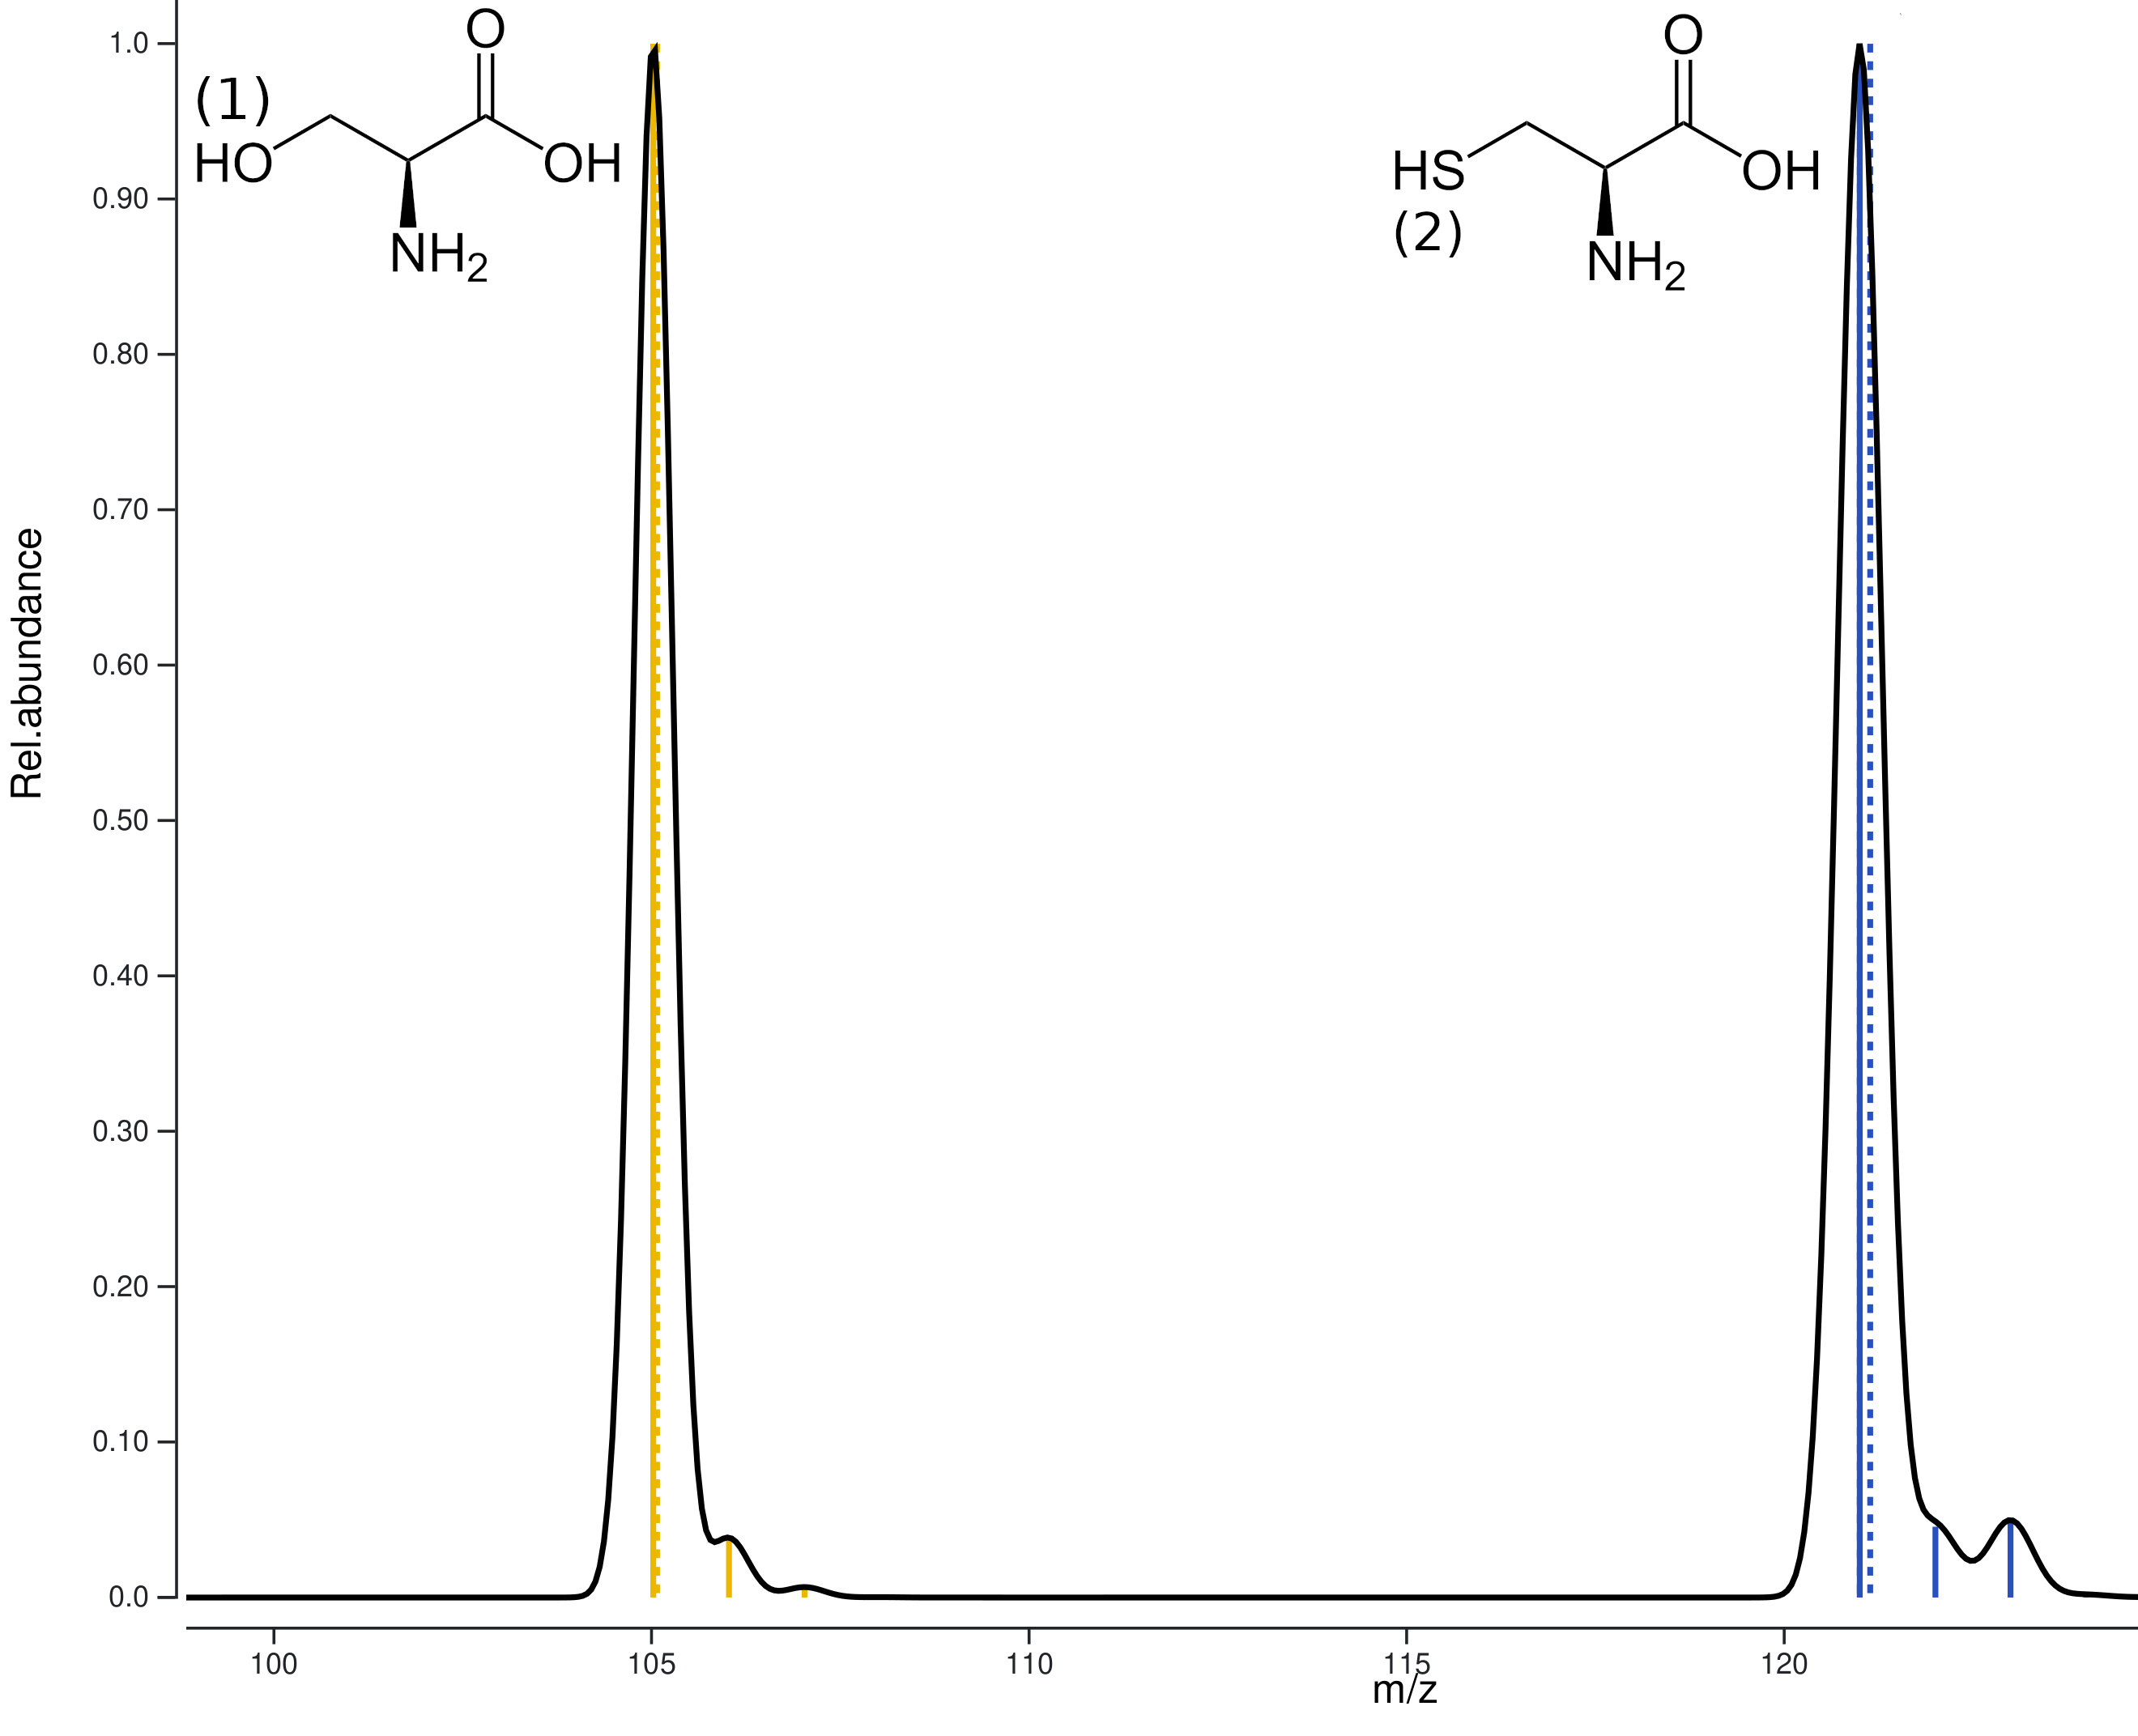
\includegraphics[width=0.75\textwidth]{./Resources/Simulated_Mass_Spectrum.png}
   \centering
   \caption{Computergeneriertes Massenspektrum von der Aminosäure \emph{Serin} (1) und \emph{Cystesin} (2). Peak von \emph{Serin} liegt bei 105; bei \emph{Systesin} um 121. y: relative Häufigkeit}
\end{figure}

Die Maxima werden \gerquot{Peaks} genannt und sind für eine Aminosäure an charakteristischer Position auf der $ x $-Achse. Obwohl sich die beiden Aminosäuren in der Abbildung \ref{fig:Sim_Mass_Spec} nur durch ein Atom unterscheiden (das linke Sauerstoffatom wurde durch ein Schwefelatom ersetzt) sind deren Massenspektren auf der $ x $-Achse weit voneinander entfernt und machen die beiden Aminosäuren dadurch sicher unterscheidbar.\\

Bei einzelnen Aminosäuren funktioniert die MS zuverlässig; bei Peptiden allerdings steht man vor dem Problem, dass das Massenspektrum unübersichtlicher wird und auch Peaks, die von Hintergrundrauschen stammen, schwerer herausgefiltert werden können. Abhilfe schafft hier die Tandem-Massenspektrometrie.

\subsection{Tandem-Massenspektrometrie (MS/MS)}\label{ss:Tandem_MS}
Bei der Tandem-Massenspektrometrie (MS/MS oder MS2) werden zwei MS Vorgänge hintereinander mit einer Probe durchgeführt. Die erste MS dient dazu Ionen aus einem bestimmten \massCharge Bereich auswählbar zu machen. Es entspricht also quasi einer Form der Filterung.

Vor der 2. MS werden die ausgewählten Reste einer Fragmentierung unterzogen. Bei einer Fragmentierung führt man Energie zu mit dem Ziel, dass die Ionen zerfallen und sog. Fragment-Ionen bilden. Diese Fragment-Ionen werden dann auf dem Massenspektrum nach der 2. MS sichtbar gemacht.

Fragment-Ionen sind kleiner als die ursprünglichen Ionen. So kann die 2. MS mit einer höheren Selektivität durchgeführt werden, welches Peaks durch Hintergrundrauschen verringert. Auch lassen sich Ionen besser identifizieren, die ein sehr ähnliches \massCharge-Verhältnis besitzen. Nach der 2. MS liegt eine Fülle an Fragment-Ionen-Peaks vor, aus denen sich die ursprünglichen Strukturinformationen ableiten lassen, da Ionen in spezifische Fragmente zerfallen \cite{Gross2013}. Zusammengefasst kann man sagen, dass das MS/MS Verfahren Ergebnisse höherer Güte erzeugt im Vergleich zur einfachen MS.

\section{De-Novo-Peptidsequenzierung mit \emph{pNovo+}}\label{s:pNovoPlusSeq}
Die \emph{pNovo+} Methode ist eine \gls{gls:DeNovo}, die mit einem \gls{gls:SpecGraph}en für die Auswertung der MS2-Spektren arbeitet und eine Erweiterung des \emph{pNovo} Verfahren darstellt \cite{pNovo}. Der Hauptansatz ist, dass zwei MS/MS Durchläufe mit jeweils verschiedenen Fragmentierungsmethoden\footnote{\emph{pNovo+} verwendet die higher energy
collisional dissociation (HCD) und die electron transfer dissociation (ETD) Fragmentierungsmethoden.} durchgeführt werden. Durch die Wahl einer anderen Fragmentierungsmethode ändert sich auch das MS2-Spektrum. Wenn nun Fragmentierungsmethoden verwendet werden, die möglichst komplementäre Spektren erzeugen, dann lässt sich durch das Zusammenführen der beiden MS2-Spektren die Qualität der Ergebnisse verbessern. Zum Beispiel lassen sich dadurch viele Peaks, die vom Hintergrundrauschen stammen, entfernen.

Für die Ermittlung der Sequenz eines Peptides wird zunächst ein Spektrums-Graph gebildet \dashAndSpace in Form eines DAG (directed acyclic graph). In diesem Graphen wird dann der längste Pfad bei gegebenen Start- und Endknoten berechnet. Die Reihenfolge der Knoten, die im längsten Pfad durchlaufen werden, stellt dann die Peptidsequenz dar.

\subsection{Vorverarbeitung der MS2-Spektren}\label{ss:Vorverarbeitung}
Bevor aus den MS2-Spektren der Spektrums-Graph gebildet werden kann, müssen die Daten vorverarbeitet werden. Für die Auswertung ist es von entscheidener Bedeutung, dass möglichst wenig Peaks verwendet werden, die vom Hintergrundrauschen stammen. Im weiteren Verlauf werden an einem exemplarischen MS2-Spektrum die Verarbeitungsschritte dargestellt.\\

Der erste Schritt ist das Verwenden des natürlichen Logarithmus der Intensitäten. Die Idee dabei ist, dass Hintergrundrauschen nicht überpriorisiert wird.

\begin{figure}[H]
   \centering
   \begin{minipage}[t]{.45\linewidth}
      \centering
      \begin{tikzpicture}[scale=\tikzScale, baseline=(current bounding box.center)]
         \draw [<->,thick] (0,\yAxisHeight) node (yaxis) [above] {\yAxisUnit}
         |- (\xAxisLength,0) node (xaxis) [right] {\xAxisUnit};
\draw[thick] (0.2, 0.0) -- (0.2, 2.3);
\draw[thick] (0.382, 0.0) -- (0.382, 1.7);
\draw[thick] (0.476, 0.0) -- (0.476, 2.7);
\draw[thick] (0.456, 0.0) -- (0.456, 1.8);
\draw[thick] (0.6859999999999999, 0.0) -- (0.6859999999999999, 2.7);
\draw[thick] (0.6839999999999999, 0.0) -- (0.6839999999999999, 1.8);
\draw[thick] (0.752, 0.0) -- (0.752, 1.1);
\draw[thick] (0.8200000000000001, 0.0) -- (0.8200000000000001, 2.2);
\draw[thick] (1.076, 0.0) -- (1.076, 1.5);
\draw[thick] (1.16, 0.0) -- (1.16, 1.9);
\draw[thick] (1.2120000000000002, 0.0) -- (1.2120000000000002, 2.0);
\draw[thick] (1.28, 0.0) -- (1.28, 1.9);
\draw[thick] (1.452, 0.0) -- (1.452, 1.3);
\draw[thick] (1.426, 0.0) -- (1.426, 1.9);
\draw[thick] (1.548, 0.0) -- (1.548, 1.9);
\draw[thick] (1.6740000000000002, 0.0) -- (1.6740000000000002, 1.5);
\draw[thick] (1.788, 0.0) -- (1.788, 2.5);
\draw[thick] (1.856, 0.0) -- (1.856, 2.3);
\draw[thick] (2.036, 0.0) -- (2.036, 1.7);
\draw[thick] (2.142, 0.0) -- (2.142, 1.6);
\draw[thick] (2.2520000000000002, 0.0) -- (2.2520000000000002, 2.0);
\draw[thick] (2.386, 0.0) -- (2.386, 1.6);
\draw[thick] (2.488, 0.0) -- (2.488, 2.9);
\draw[thick] (2.4739999999999998, 0.0) -- (2.4739999999999998, 2.7);
\draw[thick] (2.504, 0.0) -- (2.504, 2.0);
\draw[thick] (2.682, 0.0) -- (2.682, 2.0);
\draw[thick] (2.702, 0.0) -- (2.702, 2.5);
\draw[thick] (2.9259999999999997, 0.0) -- (2.9259999999999997, 2.8);
\draw[thick] (3.024, 0.0) -- (3.024, 2.4);
\draw[thick] (3.096, 0.0) -- (3.096, 1.8);
\draw[thick] (3.244, 0.0) -- (3.244, 2.6);
\draw[thick] (3.362, 0.0) -- (3.362, 1.9);
\draw[thick] (3.46, 0.0) -- (3.46, 2.3);
\draw[thick] (3.516, 0.0) -- (3.516, 1.1);
\draw[thick] (3.584, 0.0) -- (3.584, 1.8);
\draw[thick] (3.652, 0.0) -- (3.652, 2.0);
\draw[thick] (3.838, 0.0) -- (3.838, 1.5);
\draw[thick] (3.8819999999999997, 0.0) -- (3.8819999999999997, 2.6);
\draw[thick] (4.088, 0.0) -- (4.088, 2.6);
\draw[thick] (4.046, 0.0) -- (4.046, 1.1);
\draw[thick] (4.167999999999999, 0.0) -- (4.167999999999999, 2.0);
\draw[thick] (4.266, 0.0) -- (4.266, 2.4);
\draw[thick] (4.38, 0.0) -- (4.38, 1.1);
\draw[thick] (4.456, 0.0) -- (4.456, 2.2);
\draw[thick] (4.644, 0.0) -- (4.644, 2.6);
\draw[thick] (4.675999999999999, 0.0) -- (4.675999999999999, 2.5);
\draw[thick] (4.898000000000001, 0.0) -- (4.898000000000001, 1.2);
   \end{tikzpicture}%
   \end{minipage}%
   \textbf{$\rightarrow$} 
   \begin{minipage}[t]{.45\linewidth}
      \centering
      \begin{tikzpicture}[scale=\tikzScale, baseline=(current bounding box.center)]
      \draw [<->,thick] (0,\yAxisHeight) node (yaxis) [above] {\yAxisUnit}
      |- (\xAxisLength,0) node (xaxis) [right] {\xAxisUnit};
\draw[thick] (0.2, 0.0) -- (0.2, {ln(2.3)});
\draw[thick] (0.382, 0.0) -- (0.382, {ln(1.7)});
\draw[thick] (0.476, 0.0) -- (0.476, {ln(2.7)});
\draw[thick] (0.456, 0.0) -- (0.456, {ln(1.8)});
\draw[thick] (0.6859999999999999, 0.0) -- (0.6859999999999999, {ln(2.7)});
\draw[thick] (0.6839999999999999, 0.0) -- (0.6839999999999999, {ln(1.8)});
\draw[thick] (0.752, 0.0) -- (0.752, {ln(1.1)});
\draw[thick] (0.8200000000000001, 0.0) -- (0.8200000000000001, {ln(2.2)});
\draw[thick] (1.076, 0.0) -- (1.076, {ln(1.5)});
\draw[thick] (1.16, 0.0) -- (1.16, {ln(1.9)});
\draw[thick] (1.2120000000000002, 0.0) -- (1.2120000000000002, {ln(2.0)});
\draw[thick] (1.28, 0.0) -- (1.28, {ln(1.9)});
\draw[thick] (1.452, 0.0) -- (1.452, {ln(1.3)});
\draw[thick] (1.426, 0.0) -- (1.426, {ln(1.9)});
\draw[thick] (1.548, 0.0) -- (1.548, {ln(1.9)});
\draw[thick] (1.6740000000000002, 0.0) -- (1.6740000000000002, {ln(1.5)});
\draw[thick] (1.788, 0.0) -- (1.788, {ln(2.5)});
\draw[thick] (1.856, 0.0) -- (1.856, {ln(2.3)});
\draw[thick] (2.036, 0.0) -- (2.036, {ln(1.7)});
\draw[thick] (2.142, 0.0) -- (2.142, {ln(1.6)});
\draw[thick] (2.2520000000000002, 0.0) -- (2.2520000000000002, {ln(2.0)});
\draw[thick] (2.386, 0.0) -- (2.386, {ln(1.6)});
\draw[thick] (2.488, 0.0) -- (2.488, {ln(2.9)});
\draw[thick] (2.4739999999999998, 0.0) -- (2.4739999999999998, {ln(2.7)});
\draw[thick] (2.504, 0.0) -- (2.504, {ln(2.0)});
\draw[thick] (2.682, 0.0) -- (2.682, {ln(2.0)});
\draw[thick] (2.702, 0.0) -- (2.702, {ln(2.5)});
\draw[thick] (2.9259999999999997, 0.0) -- (2.9259999999999997, {ln(2.8)});
\draw[thick] (3.024, 0.0) -- (3.024, {ln(2.4)});
\draw[thick] (3.096, 0.0) -- (3.096, {ln(1.8)});
\draw[thick] (3.244, 0.0) -- (3.244, {ln(2.6)});
\draw[thick] (3.362, 0.0) -- (3.362, {ln(1.9)});
\draw[thick] (3.46, 0.0) -- (3.46, {ln(2.3)});
\draw[thick] (3.516, 0.0) -- (3.516, {ln(1.1)});
\draw[thick] (3.584, 0.0) -- (3.584, {ln(1.8)});
\draw[thick] (3.652, 0.0) -- (3.652, {ln(2.0)});
\draw[thick] (3.838, 0.0) -- (3.838, {ln(1.5)});
\draw[thick] (3.8819999999999997, 0.0) -- (3.8819999999999997, {ln(2.6)});
\draw[thick] (4.088, 0.0) -- (4.088, {ln(2.6)});
\draw[thick] (4.046, 0.0) -- (4.046, {ln(1.1)});
\draw[thick] (4.167999999999999, 0.0) -- (4.167999999999999, {ln(2.0)});
\draw[thick] (4.266, 0.0) -- (4.266, {ln(2.4)});
\draw[thick] (4.38, 0.0) -- (4.38, {ln(1.1)});
\draw[thick] (4.456, 0.0) -- (4.456, {ln(2.2)});
\draw[thick] (4.644, 0.0) -- (4.644, {ln(2.6)});
\draw[thick] (4.675999999999999, 0.0) -- (4.675999999999999, {ln(2.5)});
\draw[thick] (4.898000000000001, 0.0) -- (4.898000000000001, {ln(1.2)});
      \end{tikzpicture}
      \end{minipage}
      \caption{Anwendung des $ ln $ auf einem exemplarischen MS2-Spektrum.}
\end{figure}

Für das Verständnis des nächsten Schrittes muss man sich in Erinnerung rufen, dass eine gleiche Aminosäure keineswegs immer die gleiche Masse hat. Durch Isotope existiert eine gewisse \gerquot{Massenbandbreite} für ein und dieselbe Aminosäure. MS Systeme sind heute so genau, dass sie diese Differenzen erkennen. Dies hat den ungewollten Effekt, dass mehrere Peaks zu einer Aminosäure gehören können \cite{IsotopicDistributionMS}. Gleichzeitig können die \gerquot{Massenbandbreiten} zweier Aminosäuren sich überschneiden, sodass im ungünstigen Fall zwei Peaks kaum unterscheidbar nebeneinander liegen.\\

Eine Möglichkeit mit dieser Problematik umzugehen ist die Verwendung der monoisotopischen Masse. Die monoisotopische Masse ist die \gerquot{[...] exact mass of the most abundant naturally occurring stable isotope determined relative to the mass of 12 C, which is assigned the exact value of 12.0000.} \cite{MonoisotopicMass}. Ohne dabei jetzt tiefer ins Detail zu gehen kann man sagen, dass alle Peaks, deren Intensität mit einer möglichen monoisotopischen Masse übereinstimmen, auf jeden Fall einer Aminosäure entsprechen und (höchstwahrscheinlich)\footnote{Natürlich ist es möglich, dass das Rauschen zufällig einer monoisotopischen Masse entspricht. Die Wahrscheinlichkeit dafür ist allerdings sehr gering.} kein Hintergrundrauschen sind \cite{MassDefectMS}. Diese Peaks bekommen eine sogennante \emph{charge state}.\\

Der Algorithmus verwendet die \emph{charge state} Peaks als Ausganspunkte für weitere Berechnungen. Wenn die \massCharge Differenz zu einem anderen Peak einem Peptidfragment entspricht, dann stammt dieser Peak höchstwahrscheinlich von einem Fragment. Insgesamt werden damit die relevanten Peptidfragmente herausgeholt. Abbildung \ref{MonoisotopicMassFiltering} zeigt das Ergebnis nach den beiden zuvor genannten Schritten.

\begin{figure}[H]\label{MonoisotopicMassFiltering}
   \centering
   \begin{minipage}[t]{.45\linewidth}
      \centering
      \begin{tikzpicture}[scale=\tikzScale, baseline=(current bounding box.center)]
         \draw [<->,thick] (0,\yAxisHeight) node (yaxis) [above] {\yAxisUnit}
         |- (\xAxisLength,0) node (xaxis) [right] {\xAxisUnit};
\draw[thick] (0.2, 0.0) -- (0.2, {ln(2.3)});
\draw[color=blue!85!,opacity=.55,thick] (0.382, 0.0) -- (0.382, {ln(1.7)});
\draw[color=blue!85!,opacity=.55,thick] (0.476, 0.0) -- (0.476, {ln(2.7)});
\draw[color=magenta,thick] (0.456, 0.0) -- (0.456, {ln(1.8)});
\draw[color=blue!85!,opacity=.55,thick] (0.6859999999999999, 0.0) -- (0.6859999999999999, {ln(2.7)});
\draw[color=blue!85!,opacity=.55,thick] (0.6839999999999999, 0.0) -- (0.6839999999999999, {ln(1.8)});
\draw[thick] (0.752, 0.0) -- (0.752, {ln(1.1)});
\draw[thick] (0.8200000000000001, 0.0) -- (0.8200000000000001, {ln(2.2)});
\draw[thick] (1.076, 0.0) -- (1.076, {ln(1.5)});
\draw[thick] (1.16, 0.0) -- (1.16, {ln(1.9)});
\draw[thick] (1.2120000000000002, 0.0) -- (1.2120000000000002, {ln(2.0)});
\draw[thick] (1.28, 0.0) -- (1.28, {ln(1.9)});
\draw[color=blue!85!,opacity=.55,thick] (1.452, 0.0) -- (1.452, {ln(1.3)});
\draw[color=blue!85!,opacity=.55,thick] (1.426, 0.0) -- (1.426, {ln(1.9)});
\draw[color=magenta,thick] (1.548, 0.0) -- (1.548, {ln(1.9)});
\draw[color=blue!85!,opacity=.55,thick] (1.6740000000000002, 0.0) -- (1.6740000000000002, {ln(1.5)});
\draw[color=blue!85!,opacity=.55,thick] (1.788, 0.0) -- (1.788, {ln(2.5)});
\draw[thick] (1.856, 0.0) -- (1.856, {ln(2.3)});
\draw[thick] (2.036, 0.0) -- (2.036, {ln(1.7)});
\draw[thick] (2.142, 0.0) -- (2.142, {ln(1.6)});
\draw[thick] (2.2520000000000002, 0.0) -- (2.2520000000000002, {ln(2.0)});
\draw[thick] (2.386, 0.0) -- (2.386, {ln(1.6)});
\draw[color=blue!85!,opacity=.55,thick] (2.488, 0.0) -- (2.488, {ln(2.9)});
\draw[thick] (2.4739999999999998, 0.0) -- (2.4739999999999998, {ln(2.7)});
\draw[color=blue!85!,opacity=.55,thick] (2.504, 0.0) -- (2.504, {ln(2.0)});
\draw[color=magenta,thick] (2.682, 0.0) -- (2.682, {ln(2.0)});
\draw[color=blue!85!,opacity=.55,thick] (2.702, 0.0) -- (2.702, {ln(2.5)});
\draw[thick] (2.9259999999999997, 0.0) -- (2.9259999999999997, {ln(2.8)});
\draw[thick] (3.024, 0.0) -- (3.024, {ln(2.4)});
\draw[thick] (3.096, 0.0) -- (3.096, {ln(1.8)});
\draw[thick] (3.244, 0.0) -- (3.244, {ln(2.6)});
\draw[thick] (3.362, 0.0) -- (3.362, {ln(1.9)});
\draw[color=blue!85!,opacity=.55,thick] (3.46, 0.0) -- (3.46, {ln(2.3)});
\draw[color=blue!85!,opacity=.55,thick] (3.516, 0.0) -- (3.516, {ln(1.1)});
\draw[color=blue!85!,opacity=.55,thick] (3.584, 0.0) -- (3.584, {ln(1.8)});
\draw[color=magenta,thick] (3.652, 0.0) -- (3.652, {ln(2.0)});
\draw[color=blue!85!,opacity=.55,thick] (3.838, 0.0) -- (3.838, {ln(1.5)});
\draw[color=blue!85!,opacity=.55,thick] (3.8819999999999997, 0.0) -- (3.8819999999999997, {ln(2.6)});
\draw[thick] (4.088, 0.0) -- (4.088, {ln(2.6)});
\draw[thick] (4.046, 0.0) -- (4.046, {ln(1.1)});
\draw[thick] (4.167999999999999, 0.0) -- (4.167999999999999, {ln(2.0)});
\draw[thick] (4.266, 0.0) -- (4.266, {ln(2.4)});
\draw[color=blue!85!,opacity=.55,thick] (4.38, 0.0) -- (4.38, {ln(1.1)});
\draw[color=blue!85!,opacity=.55,thick] (4.456, 0.0) -- (4.456, {ln(2.2)});
\draw[color=magenta,thick] (4.644, 0.0) -- (4.644, {ln(2.6)});
\draw[color=blue!85!,opacity=.55,thick] (4.675999999999999, 0.0) -- (4.675999999999999, {ln(2.5)});
\draw[color=blue!85!,opacity=.55,thick] (4.898000000000001, 0.0) -- (4.898000000000001, {ln(1.2)});
   \end{tikzpicture}%
   \end{minipage}%
   \textbf{$\rightarrow$} 
   \begin{minipage}[t]{.45\linewidth}
      \centering
      \begin{tikzpicture}[scale=\tikzScale, baseline=(current bounding box.center)]
      \draw [<->,thick] (0,\yAxisHeight) node (yaxis) [above] {\yAxisUnit}
      |- (\xAxisLength,0) node (xaxis) [right] {\xAxisUnit};
\draw[color=blue!85!,opacity=.55,thick] (0.382, 0.0) -- (0.382, {ln(1.7)});
\draw[color=blue!85!,opacity=.55,thick] (0.476, 0.0) -- (0.476, {ln(2.7)});
\draw[color=magenta,thick] (0.456, 0.0) -- (0.456, {ln(1.8)});
\draw[color=blue!85!,opacity=.55,thick] (0.6859999999999999, 0.0) -- (0.6859999999999999, {ln(2.7)});
\draw[color=blue!85!,opacity=.55,thick] (0.6839999999999999, 0.0) -- (0.6839999999999999, {ln(1.8)});
\draw[color=blue!85!,opacity=.55,thick] (1.452, 0.0) -- (1.452, {ln(1.3)});
\draw[color=blue!85!,opacity=.55,thick] (1.426, 0.0) -- (1.426, {ln(1.9)});
\draw[color=magenta,thick] (1.548, 0.0) -- (1.548, {ln(1.9)});
\draw[color=blue!85!,opacity=.55,thick] (1.6740000000000002, 0.0) -- (1.6740000000000002, {ln(1.5)});
\draw[color=blue!85!,opacity=.55,thick] (1.788, 0.0) -- (1.788, {ln(2.5)});
\draw[color=blue!85!,opacity=.55,thick] (2.488, 0.0) -- (2.488, {ln(2.9)});
\draw[color=blue!85!,opacity=.55,thick] (2.504, 0.0) -- (2.504, {ln(2.0)});
\draw[color=magenta,thick] (2.682, 0.0) -- (2.682, {ln(2.0)});
\draw[color=blue!85!,opacity=.55,thick] (2.702, 0.0) -- (2.702, {ln(2.5)});
\draw[color=blue!85!,opacity=.55,thick] (3.46, 0.0) -- (3.46, {ln(2.3)});
\draw[color=blue!85!,opacity=.55,thick] (3.516, 0.0) -- (3.516, {ln(1.1)});
\draw[color=blue!85!,opacity=.55,thick] (3.584, 0.0) -- (3.584, {ln(1.8)});
\draw[color=magenta,thick] (3.652, 0.0) -- (3.652, {ln(2.0)});
\draw[color=blue!85!,opacity=.55,thick] (3.838, 0.0) -- (3.838, {ln(1.5)});
\draw[color=blue!85!,opacity=.55,thick] (3.8819999999999997, 0.0) -- (3.8819999999999997, {ln(2.6)});
\draw[color=blue!85!,opacity=.55,thick] (4.38, 0.0) -- (4.38, {ln(1.1)});
\draw[color=blue!85!,opacity=.55,thick] (4.456, 0.0) -- (4.456, {ln(2.2)});
\draw[color=magenta,thick] (4.644, 0.0) -- (4.644, {ln(2.6)});
\draw[color=blue!85!,opacity=.55,thick] (4.675999999999999, 0.0) -- (4.675999999999999, {ln(2.5)});
\draw[color=blue!85!,opacity=.55,thick] (4.898000000000001, 0.0) -- (4.898000000000001, {ln(1.2)});
      \end{tikzpicture}
      \end{minipage}
      \caption{Entfernen von Peaks, die keiner monoisotopischen Masse entsprechen oder benachbart mit einer Differenz von einem Fragment-Ion sind.}
\end{figure}

Tatsächlich ist die Verarbeitung an dieser Stelle noch etwas komplexer. So existieren auch noch sogenannte \emph{isotopic cluster}\footnote{Definition eines \emph{isotopic cluster} nach IUPAC: \gerquot{Group of peaks representing ions of the same elemental composition, but different isotopic compositions.} \cite[1556]{IUPACDefinitions}}, die gesondert verarbeitet werden. Für das grundsätzliche Prinzip ist dieses Detail allerdings weniger relevant.\\

Im letzten Vorberarbeitungsschritt werden Peaks aus einem irrelevanten \massCharge Bereich entfernt und naheliegende Peaks werden zusammengefasst, indem der Mittelwert sowol des \massCharge Wertes als auch der der Intensität besimmt wird. Üblicherweise liegt der Bereich für das Zusammenfassen bei $ +- 20 ppm $.

\begin{figure}[H]
   \centering
   \begin{minipage}[t]{.45\linewidth}
      \centering
      \begin{tikzpicture}[scale=\tikzScale, baseline=(current bounding box.center)]
         \draw [<->,thick] (0,\yAxisHeight) node (yaxis) [above] {\yAxisUnit}
         |- (\xAxisLength,0) node (xaxis) [right] {\xAxisUnit};
\draw[thick] (0.382, 0.0) -- (0.382, {ln(1.7)});
\draw[thick] (0.476, 0.0) -- (0.476, {ln(2.7)});
\draw[thick] (0.456, 0.0) -- (0.456, {ln(1.8)});
\draw[thick] (0.6859999999999999, 0.0) -- (0.6859999999999999, {ln(2.7)});
\draw[thick] (0.6839999999999999, 0.0) -- (0.6839999999999999, {ln(1.8)});
\draw[color=red,thick] (1.452, 0.0) -- (1.452, {ln(1.3)});
\draw[color=red,thick] (1.426, 0.0) -- (1.426, {ln(1.9)});
\draw[thick] (1.548, 0.0) -- (1.548, {ln(1.9)});
\draw[thick] (1.6740000000000002, 0.0) -- (1.6740000000000002, {ln(1.5)});
\draw[thick] (1.788, 0.0) -- (1.788, {ln(2.5)});
\draw[color=red,thick] (2.488, 0.0) -- (2.488, {ln(2.9)});
\draw[color=red,thick] (2.504, 0.0) -- (2.504, {ln(2.0)});
\draw[color=red,thick] (2.682, 0.0) -- (2.682, {ln(2.0)});
\draw[color=red,thick] (2.702, 0.0) -- (2.702, {ln(2.5)});
\draw[thick] (3.46, 0.0) -- (3.46, {ln(2.3)});
\draw[thick] (3.516, 0.0) -- (3.516, {ln(1.1)});
\draw[thick] (3.584, 0.0) -- (3.584, {ln(1.8)});
\draw[thick] (3.652, 0.0) -- (3.652, {ln(2.0)});
\draw[color=red,thick] (3.838, 0.0) -- (3.838, {ln(1.5)});
\draw[color=red,thick] (3.8819999999999997, 0.0) -- (3.8819999999999997, {ln(2.6)});
\draw[thick] (4.38, 0.0) -- (4.38, {ln(1.1)});
\draw[thick] (4.456, 0.0) -- (4.456, {ln(2.2)});
\draw[thick] (4.644, 0.0) -- (4.644, {ln(2.6)});
\draw[thick] (4.675999999999999, 0.0) -- (4.675999999999999, {ln(2.5)});
\draw[thick] (4.898000000000001, 0.0) -- (4.898000000000001, {ln(1.2)});

\fill[red!25!,opacity=.25] (0,0) rectangle (1,\yAxisHeight-\axisColorOffset);
         \fill[red!25!,opacity=.25] (\xAxisLength-1,0) rectangle (\xAxisLength-\axisColorOffset,\yAxisHeight-\axisColorOffset);
         \fill[green!25!,opacity=.25] (1,0) rectangle (\xAxisLength-1,\yAxisHeight-\axisColorOffset);
   \end{tikzpicture}%
   \end{minipage}%
   \textbf{$\rightarrow$} 
   \begin{minipage}[t]{.45\linewidth}
      \centering
      \begin{tikzpicture}[scale=\tikzScale, baseline=(current bounding box.center)]
      \draw [<->,thick] (0,\yAxisHeight) node (yaxis) [above] {\yAxisUnit}
      |- (\xAxisLength,0) node (xaxis) [right] {\xAxisUnit};
%\draw[color=red,thick] (1.452, 0.0) -- (1.452, {ln(1.3)});
%\draw[color=red,thick] (1.426, 0.0) -- (1.426, {ln(1.9)});
\draw[color=red,ultra thick] ({(1.452+1.426)/2}, 0.0) -- ({(1.452+1.426)/2}, {(ln(1.3)+ln(1.9))/2});

\draw[thick] (1.548, 0.0) -- (1.548, {ln(1.9)});
\draw[thick] (1.6740000000000002, 0.0) -- (1.6740000000000002, {ln(1.5)});
\draw[thick] (1.788, 0.0) -- (1.788, {ln(2.5)});

%\draw[color=red,thick] (2.488, 0.0) -- (2.488, {ln(2.9)});
%\draw[color=red,thick] (2.504, 0.0) -- (2.504, {ln(2.0)});
\draw[color=red,ultra thick] ({(2.488+2.504)/2}, 0.0) -- ({(2.488+2.504)/2}, {(ln(2.9)+ln(2.0))/2});

%\draw[color=red,thick] (2.682, 0.0) -- (2.682, {ln(2.0)});
%\draw[color=red,thick] (2.702, 0.0) -- (2.702, {ln(2.5)});
\draw[color=red,ultra thick] ({(2.682+2.702)/2}, 0.0) -- ({(2.682+2.702)/2}, {(ln(2.0+ln(2.5))/2});

\draw[thick] (3.46, 0.0) -- (3.46, {ln(2.3)});
\draw[thick] (3.516, 0.0) -- (3.516, {ln(1.1)});
\draw[thick] (3.584, 0.0) -- (3.584, {ln(1.8)});
\draw[thick] (3.652, 0.0) -- (3.652, {ln(2.0)});

%\draw[color=red,thick] (3.838, 0.0) -- (3.838, {ln(1.5)});
%\draw[color=red,thick] (3.8819999999999997, 0.0) -- (3.8819999999999997,{ln(2.6)});
\draw[color=red,ultra thick] ({(3.838+3.8819999999999997)/2}, 0.0) -- ({(3.838+3.8819999999999997)/2}, {(ln(1.5)+ln(2.6))/2});

\fill[red!25!,opacity=.25] (0,0) rectangle (1,\yAxisHeight-\axisColorOffset);
         \fill[red!25!,opacity=.25] (\xAxisLength-1,0) rectangle (\xAxisLength-\axisColorOffset,\yAxisHeight-\axisColorOffset);
         \fill[green!25!,opacity=.25] (1,0) rectangle (\xAxisLength-1,\yAxisHeight-\axisColorOffset);
      \end{tikzpicture}
      \end{minipage}
      \caption{Entfernen von Peaks aus einem irrelevanten \massCharge Bereich und zusammenfassen naheliegender Peaks. Rot markierte Peaks sind jene, die zusammengefasst werden.}
\end{figure}

\subsection{Bildung eines Spektrums-Graphen}\label{ss:BildungSpekGraph}
Der Spektrums-Graph wird aus einem vorverarbeiteten MS2-Spektrum (siehe Kapitel: \ref{ss:Vorverarbeitung}) gebildet. Im initialen Zustand werden die Peaks als Knoten interpretiert. Dazu kommt ein Start- und Endknoten. Jedem Knoten wird eine Masse zugeordet; im initialen Zustand bekommt der Startknoten die Masse 0 und der Endknoten die Masse des vorherigen Knotens minus der Masse des Wassers ($ 18,02 $). Die Masse der übrigen Knoten entsprechen ihren jeweils korrespondierenden \massCharge Wert. Die gerichteten Kanten werden zwischen einem Knotenpaar hinzugefügt, wenn die Differenz deren Masse gleich ist mit der Masse von ein oder zwei Aminosäuren.

\subsection{Identifikation der Aminosäuresequenz}
Der gebildete DAG kann mit klassischen Algorithmen, die den längsten Pfad suchen, durchlaufen werden. Bezogen auf die Graphentheorie entspricht die Ermittlung der Aminosäurensequenz dem Suchen eines bestimmten Pfades \dashAndSpace und nicht nach irgendeinem Pfad. Daher muss der Algorithmus mittels einer Breitensuche arbeiten, um alle möglichen Pfade zu bestimmen.

In aller Regel wird es mehrere Pfade geben. Bestimmte Sequenzen sind wahrscheinlicher als andere. So sind Pfade mit Kanten, die wegen der Massendifferenz von genau einer Aminosäure gebildet wurden, wahrscheinlicher \cite{pNovoPlus}. Alle Pfade bekommen mittels einer Scoring-Funktion einen Wert zugewiesen. Der Pfad mit dem höchsten Scoring-Wert ist wahrscheinlich das richtige Ergebnis. Die Scoring-Funktion berücksichtigt unter anderem wie viele Fragmente, die einer bestimmten Aminosäure zugeordet werden können, im MS2-Spektrum vorhanden sind \cite{pNovo}. Die Sequenz mit dem höchsten Scoring-Wert ist das Endergebnis.

\section{De-Novo-Peptidsequenzierung mit \emph{Open-pNovo}}\label{s:OpenpNovoSeq}
Bei Proteinen können posttranslationale Proteinmodifikationen (PTM) auftreten. PTMs sind Ereignisse, bei denen sich Änderungen im Protein einstellen \cite{Mann2003}; teilweise sind die Änderungen von einer Zelle erwünscht \dashAndSpace teilweise stammen sie aber auch zum Beispiel von unerwünschten Wechselwirkungen nebeneinanderliegenden Aminosäuren. Ein Teil dieser PTMs führen zu einer Änderung der Aminosäuresequenz. Dies ist für die \gls{gls:DeNovo} nicht weiter problematisch, da sowieso ohne eine Datenbank gearbeitet wird, sodass solche PTMs nicht einmal auffallen würden. Andere PTMs hingegen haben die Auswirkung, dass Stoffe gebildet werden, die nicht mehr zu der Gruppe der proteinogenen Aminosäuren gehören. Proteinogene Aminosäuren sind jene Aminosäuren, die für den Bau von Proteinen verwendet werden. Der Effekt ist also, dass Stoffe (oder deren Fragmente) bei einem Massenspektrum angezeigt werden, die kein Teil eines Peptids sein können. Bei der Sequenzierung von Peptidfragmenten muss dies daher berücksichtigt werden.
Wenn im weiteren Verlauf von PTMs gesprochen wird, dann sind solche gemeint, die für die \gls{gls:DeNovo} relevant sind.

Open-pNovo ist ein \gls{gls:DeNovo}sverfahren, welches auf pNovo+ Tool aufbaut und versucht die Problematik mit den PTMs zu lösen.

\subsection{PTMs im konstruierten DAG}
Die Konvertierung eines MS2-Spektrums läuft bis zum DAG analog ab wie in den Kapiteln \ref{ss:Vorverarbeitung} und \ref{ss:BildungSpekGraph} für pNovo+. Der Unterschied ist nun, dass es zwei Arten von Kanten gibt:

\begin{itemize}
   \item \gerquot{Normale} Kanten: Kanten, die gebildet werden, wie es bereits für \emph{pNovo+} gezeigt wurde. 
   \item \gerquot{Modifizierte} Kanten: Kanten, die zum Grahpen hinzugefügt werden, wenn die Massendifferenz zweier Knoten der Masse einer Aminosäure plus der Masse einer möglichen PTM-Änderung entspricht. 
\end{itemize}

Eine Liste aller PTMs in der Datenbank Unimod (sowohl relevante als auch nicht relevante) beinhaltet aktuell 1510 Einträge\footnote{Siehe: \url{https://www.ebi.ac.uk/ols/ontologies/unimod}} (Stand: 18.04.2022). Für die modifizierten Kanten gibt es insgesamt $ 1510 * 20 = 30200 $ mögliche Differenzen, wobei viele davon nicht relevante PTMs sind. Zum Vergleich: bei den normalen Kanten gibt es $ 20^2 = 400 $ mögliche Differenzen.

Die hohe Anzahl an Differenzen für modifizierte Kanten hat die Konsequenz, dass viele Knoten zufällig verbunden werden und dass dadurch die Genauigkeit der Ergebnisse abnimmt. Dieses Problem kann man durch eine geringere Liste an möglichen PTMs abfedern, allerdings mit einem Verlust  der Genauigkeit auf Seiten der PTMs. Es ist hier also eine Abwägung.

\subsection{Evaluierung von Open-pNovo}
Open-pNovo wurde sowohl auf drei realen als auch auf drei generierten Testdaten getestet. Tabelle \ref{tab:OpenPNovoResults} zeigt die Ergebnisse im Vergleich zu pNovo+ und zwei anderen Algorithmen. Die Datensätze enthielten die am häufigsten vorkommenden PTMs.

\begin{table}[H]
    \centering
    \begin{tabular}{l|c|c|c|c}
        \toprule
        \textbf{Testdatensätze} & \textbf{Open-pNovo+} & \textbf{pNovo+} & \textbf{PEAKS} & \textbf{Novor} \\
        \midrule
        Real (20259) & $76,3 \%$ & $68,5 \%$ & $65,8 \%$ & $39,9 \%$ \\
        Generiert (17877) & $77,8 \%$ & $0,6 \%$ & $0,5 \%$ & $0,2 \%$ \\
        \bottomrule
    \end{tabular}
    \newline
    \caption{Vergleich der durchschnittlichen richtigen \gls{gls:DeNovo} Peptidsequenzierungen von Open-pNovo und anderen Algorithmen \cite[650]{OpenPNovo}.}
    \label{tab:OpenPNovoResults}
\end{table}

Die enorm schlechten Ergebnisse der anderen Algorithmen bei den generierten Testdaten ist ein Nebeneffekt des Ziels bei der Testdatengenerierung. Denn diese wurden so ausgelegt, um die Grenzen von Open-pNovo+ zu ermitteln \cite[649]{OpenPNovo}. Eine Aussagekraft haben diese Ergebnisse also nicht. Allerdings auch bei realen Testdaten zeigt sich Open-pNovo als voll konkurrenzfähig gegenüber den anderen Algorithmen.

Noch besser zeigt sich Open-pNovo, wenn der Recall Wert betrachtet wird \dashAndSpace also die Anzahl an verschiedenen PSMs, die erkannt wurden. In diesem Fall ist der Abstand zu den anderen Algorithmen deutlich größer geworden.

\begin{table}[H]
    \centering
    \begin{tabular}{l|c|c|c|c}
        \toprule
        \textbf{Testdatensätze} & \textbf{Open-pNovo+} & \textbf{pNovo+} & \textbf{PEAKS} & \textbf{Novor} \\
        \midrule
        Real (5034) & $61,6 \%$ & $31,3 \%$ & $32,0 \%$ & $13,7 \%$ \\
        \bottomrule
    \end{tabular}
    \newline
    \caption{Vergleich der durchschnittlichen Recall Werte einer \gls{gls:DeNovo} Peptidsequenzierungen von Open-pNovo und anderen Algorithmen \cite[650]{OpenPNovo}.}
    \label{tab:OpenPNovoResultsRecall}
\end{table}

\subsection{Zusammenfassung}


% Die \gls{gls:DeNovo} nutzt die sogenannte \gls{gls:TMassSpek} für die Bestimmung der Peptidsequenz. Dabei wird die physikalische Eigenschaft ausgenutzt, dass jedes Atom bzw. jedes Molekül \dashAndSpace wenn es einer \gls{gls:Ionisation} unterzogen wurde \dashAndSpace ein charakteristisches \gls{gls:MassSpek} besitzt. Das \gls{gls:MassSpek} stellt also eine Art \gerquot{Fingerabdruck} eines Moleküls dar und macht dieses ermittelbar.

% U.U. eine Beispielgrafik eines Massenspektrums hinzufuegen ...

\subsubsection{\glsentrytext{gls:TMassSpek} bei größeren Molekülen}
Bei größeren Molekülen (wie einem Protein) führt die \gls{gls:Ionisation} dazu, dass das Molekül in kleinere spezifische Ionen zerfällt (sog. Fragmentierung). Die Fragmentierungsinformationen einer \gls{gls:DeNovo} sind meist unvollständig, da fehlende Daten bei einem Fragmentierungsschritt die Güte des Endergebnisses negativ beeinflusst. Dies wird insbesondere dann ein Problem, wenn unbekannte Änderungen in einer Peptidsequenz vorhanden sind.

Um dieses Problem zu verringern können unterschiedliche Techniken parallel eingesetzt werden, welche verschiedene Fragmente erzeugen und daher auch verschiedenartige \glspl{gls:MassSpek} zur Folge haben.\footnote{Konkret: Es wird sowohl das \gls{acr:HCD} als auch das \gls{acr:ETD} Verfahren angewendet.}

\subsection{Datenaufbereitung}
Typischerweise betrachtet man die sog. \gerquot{\glspl{gls:Peak}} in den \glspl{gls:MassSpek}. Jeder \gls{gls:Peak} stellt ein unterschiedliches Ion dar. Dazu kommen Messungenauigkeiten sowie Hintergrundrauschen. Durch die hohe Anzahl an möglichen Ionen kann nicht ohne weiteres differenziert werden, welcher der \glspl{gls:Peak} von welchen Ionen erzeugt wurden und welche nicht.

% Frage an Dominik: Ist hier eine einfache Auflistung an Techniken für die Datenaufbereitung besser?
Der Algorithmus für die Datenaufbereitung berechnet den natürlichen Logarithmus von den Intensitäten der \glspl{gls:Peak}, um Hintergrundrauschen und Messungenauigkeiten nicht überzupriorisieren. Zusätzlich dazu werden \glspl{gls:Peak}, die in einem Toleranzbereich nebeneinander liegen, zusammengefasst. Am Ende werden die \glspl{gls:Peak} entfernt, bei denen bekannt ist, dass es sich nicht um relevante Ionen handeln kann. (z.B. \glspl{gls:Peak} von Isotopen)

\begin{figure}[H]
   \centering
   \begin{minipage}[t]{.4\linewidth}
      \centering
      \begin{tikzpicture}[scale=\tikzScale, baseline=(current bounding box.center)]
         \draw [<->,thick] (0,2.75) node (yaxis) [above] {\yAxisUnit}
         |- (3,0) node (xaxis) [right] {\xAxisUnit};

         \draw[thick] (0.2,0) -- (0.2,1.1);
         \draw[thick] (0.3,0) -- (0.3,1.6);
         \draw[thick] (0.6,0) -- (0.6,1.7);
         \draw[thick] (0.8,0) -- (0.8,1.2);
         \draw[thick] (1.0,0) -- (1.0,1.1);

         \draw[color=red,thick] (1.2,0) -- (1.2,2.65);
         \draw[thick] (1.4,0) -- (1.4,1.4);
         \draw[thick] (1.6,0) -- (1.6,1.2);
         \draw[thick] (1.8,0) -- (1.8,1.3);
         \draw[thick] (2.0,0) -- (2.0,1.8);

         \draw[thick] (1.1,0) -- (1.1,2.0);
         \draw[color=red,thick] (0.35,0) -- (0.35,2.25);
         \draw[thick] (1.9,0) -- (1.9,1.4);
         \draw[color=red,thick] (2.2,0) -- (2.2,2.6);
         \draw[thick] (2.5,0) -- (2.5,1.25);

         \draw[thick] (2.7,0) -- (2.7,1.1);
         \foreach \x in {1,...,6}
         {
            \draw[thick] (1.2+\x*0.05,0) -- (1.2+\x*0.05,1.0+\x*0.15);
         }
      \end{tikzpicture}%
      % \subcaption{Exemplarische Rohdaten}
   \end{minipage}%
   \textbf{$\rightarrow$}
   \begin{minipage}[t]{.4\linewidth}
      \centering
      \begin{tikzpicture}[scale=\tikzScale, baseline=(current bounding box.center)]
         \draw [<->,thick] (0,2.75) node (yaxis) [above] {\yAxisUnit}
         |- (3,0) node (xaxis) [right] {\xAxisUnit};

         \draw[thick] (0.2,0) -- (0.2,{ln(1.1)});
         \draw[thick] (0.3,0) -- (0.3,{ln(1.6)});
         \draw[thick] (0.6,0) -- (0.6,{ln(1.7)});
         \draw[thick] (0.8,0) -- (0.8,{ln(1.2)});
         \draw[thick] (1.0,0) -- (1.0,{ln(1.1)});

         \draw[color=red,thick] (1.2,0) -- (1.2,{ln(2.65)});
         \draw[thick] (1.4,0) -- (1.4,{ln(1.4)});
         \draw[thick] (1.6,0) -- (1.6,{ln(1.2)});
         \draw[thick] (1.8,0) -- (1.8,{ln(1.3)});
         \draw[thick] (2.0,0) -- (2.0,{ln(1.8)});

         \draw[thick] (1.1,0) -- (1.1,{ln(2.0)});
         \draw[color=red,thick] (0.35,0) -- (0.35,{ln(2.25)});
         \draw[thick] (1.9,0) -- (1.9,{ln(1.4)});
         \draw[color=red,thick] (2.2,0) -- (2.2,{ln(2.6)});
         \draw[thick] (2.5,0) -- (2.5,{ln(1.25)});

         \draw[thick] (2.7,0) -- (2.7,{ln(1.1)});
         \foreach \x in {1,...,6}
         {%
            \draw[thick] (1.2+\x*0.05,0) -- (1.2+\x*0.05,{ln(1.0+\x*0.15)});
         }
      \end{tikzpicture}
      %\subcaption{Exemplarische Rohdaten}
   \end{minipage}
   \caption{Anwendung des $ln$ auf Rohdaten. Rote \glspl{gls:Peak} stellen hier exemplarisch fehlerhafte Daten dar, die nach dem $ln$ reduziert wurden.}
\end{figure}

\begin{figure}[H]
   \centering
   \begin{minipage}[t]{.4\linewidth}
      \centering
      \begin{tikzpicture}[scale=\tikzScale, baseline=(current bounding box.center)]
         \draw [<->,thick] (0,2.75) node (yaxis) [above] {\yAxisUnit}
         |- (3,0) node (xaxis) [right] {\xAxisUnit};

         \draw[thick] (0.2,0) -- (0.2,{ln(1.1)});
         \draw[thick] (0.3,0) -- (0.3,{ln(1.6)});
         \draw[thick] (0.6,0) -- (0.6,{ln(1.7)});
         \draw[thick] (0.8,0) -- (0.8,{ln(1.2)});
         \draw[thick] (1.0,0) -- (1.0,{ln(1.1)});

         \draw[thick] (1.2,0) -- (1.2,{ln(2.65)});
         \draw[thick] (1.4,0) -- (1.4,{ln(1.4)});
         \draw[thick] (1.6,0) -- (1.6,{ln(1.2)});
         \draw[thick] (1.8,0) -- (1.8,{ln(1.3)});
         \draw[thick] (2.0,0) -- (2.0,{ln(1.8)});

         \draw[thick] (1.1,0) -- (1.1,{ln(2.0)});
         \draw[thick] (0.35,0) -- (0.35,{ln(2.25)});
         \draw[thick] (1.9,0) -- (1.9,{ln(1.4)});
         \draw[thick] (2.2,0) -- (2.2,{ln(2.6)});
         \draw[thick] (2.5,0) -- (2.5,{ln(1.25)});

         \draw[thick] (2.7,0) -- (2.7,{ln(1.1)});
         \foreach \x in {1,...,6}
         {%
            \draw[color=red,thick] (1.2+\x*0.05,0) -- (1.2+\x*0.05,{ln(1.0+\x*0.15)});
         }

         \draw[dotted] (0.4,0) -- (0.4,2.75);
         \draw[dotted] (2.6,0) -- (2.6,2.75);
         \fill[red!25!,opacity=.25] (0,0) rectangle (0.4,2.75);
         \fill[red!25!,opacity=.25] (2.6,0) rectangle (3.0,2.75);
         \fill[green!25!,opacity=.25] (0.4,0) rectangle (2.6,2.75);
      \end{tikzpicture}
      %\subcaption{Exemplarische Rohdaten}
   \end{minipage}
   \textbf{$\rightarrow$}
   \begin{minipage}[t]{.4\linewidth}
      \centering
      \begin{tikzpicture}[scale=\tikzScale, baseline=(current bounding box.center)]
         \draw [<->,thick] (0,2.75) node (yaxis) [above] {\yAxisUnit}
         |- (3,0) node (xaxis) [right] {\xAxisUnit};

         \draw[thick] (0.6,0) -- (0.6,{ln(1.7)});
         \draw[thick] (0.8,0) -- (0.8,{ln(1.2)});
         \draw[thick] (1.0,0) -- (1.0,{ln(1.1)});

         \draw[thick] (1.2,0) -- (1.2,{ln(2.65)});
         %\draw[thick] (1.4,0) -- (1.4,{ln(1.4)});
         \draw[thick] (1.6,0) -- (1.6,{ln(1.2)});
         \draw[thick] (1.8,0) -- (1.8,{ln(1.3)});
         \draw[thick] (2.0,0) -- (2.0,{ln(1.8)});

         \draw[thick] (1.1,0) -- (1.1,{ln(2.0)});
         \draw[thick] (1.9,0) -- (1.9,{ln(1.4)});
         \draw[thick] (2.2,0) -- (2.2,{ln(2.6)});
         \draw[thick] (2.5,0) -- (2.5,{ln(1.25)});

         \draw[color=red,ultra thick] (1.2+1*0.05,0) -- (1.2+1*0.05,{ln(1.0+1*0.15)});
         \draw[color=red,ultra thick] (1.2+3*0.05,0) -- (1.2+3*0.05,{ln(1.0+3*0.15)});
         \draw[color=red,ultra thick] (1.2+5*0.05,0) -- (1.2+5*0.05,{ln(1.0+5*0.15)});

         \draw[dotted] (0.4,0) -- (0.4,2.75);
         \draw[dotted] (2.6,0) -- (2.6,2.75);
         \fill[red!25!,opacity=.25] (0,0) rectangle (0.4,2.75);
         \fill[red!25!,opacity=.25] (2.6,0) rectangle (3.0,2.75);
         \fill[green!25!,opacity=.25] (0.4,0) rectangle (2.6,2.75);
      \end{tikzpicture}
      %\subcaption{Exemplarische Rohdaten}
   \end{minipage}
   \caption{Entfernen von irrelevanten \glspl{gls:Peak} sowie zusammenfassen naheliegender \glspl{gls:Peak}. Hier symbolisieren die roten \glspl{gls:Peak} jene, die zusammengefasst werden.}
\end{figure}

% `\glsentrytext` funktioniert nicht für `\glspl`
\subsection{Konvertierung von \glspl{gls:MassSpek}}
Das Ziel der Konvertierung ist das Erzeugen eines \gls{gls:SpecGraph}en. Um von einem \gls{gls:MassSpek} zu einem \gls{gls:SpecGraph}en zu kommen, werden die \glspl{gls:Peak}, die nach der Datenaufbereitung (Siehe ...) übrig bleiben, als Knoten gewertet. Dazu kommt ein Start- und Endknoten. Jeder Knoten bekommt eine Gewichtung; diese Gewichtung entspricht der Stärke des \gls{gls:Peak}s.

\newcommand{\colorA}{white!30!green}
\newcommand{\colorB}{black!10!yellow}
\newcommand{\colorC}{white!40!red}
\newcommand{\colorD}{white!25!orange}
\newcommand{\colorE}{white!45!blue}
\newcommand{\colorF}{white!5!magenta}
\newcommand{\nodeFontSize}{\scriptsize}
\newcommand{\nodeScaleFactor}{100}
\newcommand{\round}[1]{\pgfmathprintnumber[precision=0]{#1}}
\newcommand{\rawA}{ln(1.7)}
\newcommand{\rawB}{ln(2.0)}
\newcommand{\rawC}{ln(2.65)}
\newcommand{\rawD}{ln(1.0+5*0.15)}
\newcommand{\rawE}{ln(1.85)}
\newcommand{\rawF}{ln(2.6)}
\newcommand{\valueA}{\pgfmathparse{int(\rawA*\nodeScaleFactor)}\pgfmathresult}
\newcommand{\valueB}{\pgfmathparse{int(\rawB*\nodeScaleFactor)}\pgfmathresult}
\newcommand{\valueC}{\pgfmathparse{int(\rawC*\nodeScaleFactor)}\pgfmathresult}
\newcommand{\valueD}{\pgfmathparse{int(\rawD*\nodeScaleFactor)}\pgfmathresult}
\newcommand{\valueE}{\pgfmathparse{int(\rawE*\nodeScaleFactor)}\pgfmathresult}
\newcommand{\valueF}{\pgfmathparse{int(\rawF*\nodeScaleFactor)}\pgfmathresult}

\begin{figure}[htb]
   \centering
      \begin{tikzpicture}[scale=\tikzScale*1.5, baseline=(current bounding box.center)]
         \draw [<->,thick] (0,2.75) node (yaxis) [above] {\yAxisUnit}
         |- (3,0) node (xaxis) [below] {\xAxisUnit};

         \draw[thick] (0.6,0) -- (0.6,{ln(1.7)}) node [right, rotate=90, color=\colorA] {\nodeFontSize\textbf{A} \valueA};
         \draw[thick] (0.8,0) -- (0.8,{ln(1.2)});
         \draw[thick] (1.0,0) -- (1.0,{ln(1.1)});

         \draw[thick] (1.2,0) -- (1.2,{ln(2.65)}) node [right, rotate=90,
         color=\colorC] {\nodeFontSize\textbf{C} \valueC};
         \draw[thick] (1.4,0) -- (1.4,{ln(1.4)});
         \draw[thick] (1.6,0) -- (1.6,{ln(1.2)});
         \draw[thick] (1.8,0) -- (1.8,{ln(1.3)});
         \draw[thick] (2.0,0) -- (2.0,{ln(1.8)}) node [right, rotate=90, color=\colorE] {\nodeFontSize\textbf{E} \valueE};

         \draw[thick] (1.025,0) -- (1.025,{ln(2.0)}) node [right, rotate=90, color=\colorB] {\nodeFontSize\textbf{B} \valueB};
         \draw[thick] (1.9,0) -- (1.9,{ln(1.4)});
         \draw[thick] (2.2,0) -- (2.2,{ln(2.6)}) node [right, rotate=90, color=\colorF] {\nodeFontSize\textbf{F} \valueF};
         \draw[thick] (2.5,0) -- (2.5,{ln(1.25)});

         \draw[thick] (1.2+1*0.05,0) -- (1.2+1*0.05,{ln(1.0+1*0.15)});
         \draw[thick] (1.2+3*0.05,0) -- (1.2+3*0.05,{ln(1.0+3*0.15)});
         \draw[thick] (1.2+5*0.05,0) -- (1.2+5*0.05,{ln(1.0+5*0.15)}) node [right, rotate=90, color=\colorD] {\nodeFontSize\textbf{D} \valueD};
      \end{tikzpicture}
      \caption{Ausgewählte \glspl{gls:Peak} mit einem exemplarischen x Wert.}
\end{figure}

\newcommand{\modVal}{4}

Gerichtete Kanten zwischen den Knoten werden ausgebildet, wenn diese eine Differenz von genau einer oder zwei Aminosäurereste\footnote{Da eine Aminosäure vielerlei an Reste besitzen kann, ergeben sich mehr als 40 Differenzen, die diese Bedingung erfüllen.} besitzen. Der Einfachheit halber wird im folgenden eine Kante ausgebildet, wenn die Differenz genau \textbf{\modVal} \space beträgt.

% Um einzele Knotennamen einzufärben: \textcolor{\colorA}{A}
\newcommand{\findRaw}[1]{\csname raw#1\endcsname}
\newcommand{\findValue}[1]{\csname value#1\endcsname}
\newcommand{\findColor}[1]{\csname color#1\endcsname}
\newcommand{\cmark}{\ding{51}}
\newcommand{\xmark}{\ding{55}}
\newcommand{\tableRow}[2]
{%
   % Welche Zeile soll farblich hinterlegt werden ?
   \pgfmathparse{Mod(abs(int(\findRaw{#1}*\nodeScaleFactor) - int(\findRaw{#2}*\nodeScaleFactor)),\modVal)}
   \pgfmathtruncatemacro\myresult{\pgfmathresult==0.0?1:0}
   %\ifthenelse{\myresult=1}{A}{B}
   \ifnum\myresult=1 A \else B \fi

   (#1,#2) &
   \findValue{#1} &
   \findValue{#2} &
   \pgfmathparse{abs(int(\findRaw{#1}*\nodeScaleFactor) - int(\findRaw{#2}*\nodeScaleFactor))}\round{\pgfmathresult} &

   % Hilfreiche Infos für das Erstellen von Ausdrücken: https://tikz.dev/math-parsing
   \pgfmathparse{Mod(abs(int(\findRaw{#1}*\nodeScaleFactor) - int(\findRaw{#2}*\nodeScaleFactor)),\modVal)}
   % https://www.reddit.com/r/LaTeX/comments/57ck5p/tikz_which_conditionals_to_use_to_compare_numbers/
   \pgfmathtruncatemacro\myresult{\pgfmathresult==0.0?1:0}
   \round{\pgfmathresult}
   \ifthenelse{\myresult=1}{\cmark}{\xmark}
   \\
}
% Hilfestellung: https://tex.stackexchange.com/questions/604496/how-to-generate-beautiful-tables-in-latex
\begin{table}[H]
    \centering
    \begin{tabular}{lllcc}
        \toprule
        \thead{\textbf{$\mathbf{(u,v)}$}} & \thead{$\mathbf{u}$} & \thead{$\mathbf{v}$} & \thead{$\mathbf{\Delta(u,v)}$} & \thead{$\Delta(u,v)\bmod\modVal$}\\
        \midrule
        \tableRow{A}{B}
        \tableRow{A}{C}
        \tableRow{A}{D}
        \tableRow{A}{E}
        \tableRow{A}{F}
        \tableRow{B}{C}
        \tableRow{B}{D}
        \tableRow{B}{E}
        \tableRow{B}{F}
        \tableRow{C}{D}
        \tableRow{C}{E}
        \tableRow{C}{F}
        \tableRow{D}{E}
        \tableRow{D}{F}
        \tableRow{E}{F}
        \bottomrule
    \end{tabular}
    \caption{Bestimmung der Kanten}
\end{table}

Darstellung der Daten als gewichteter, gerichteter azyklischer Graph. Zusätzlich benötigt der Graph noch separate Start- und Zielknoten; diese sind für die späteren Berechnungen unerlässlich.

\newcommand{\printVertices}[2]%
{%
   \Vertex[x=-8,y=0]{Start}
   \Vertex[x=8,y=0]{End}
   \foreach \x [count=\xi] in {#1}
   {%
      \foreach \y [count=\yi] in {#2}
      {%
         \ifthenelse{\xi=\yi}{
         \tikzstyle{VertexStyle}=[shape=circle,fill=\y,draw=black,line width=0.75pt]
         \Vertex[x=-7+\xi*2,y=0]{\x}}{\break}
      }
   }
}
% https://tex.stackexchange.com/questions/245448/adjusting-edge-and-vertex-label
\begin{figure}[htb]
   \centering
   \begin{tikzpicture}[scale=0.75,transform shape]
      \tikzstyle{VertexStyle}=[shape=circle,fill=white,draw=black,line width=1pt]

      \printVertices{A,B,C,D,E,F}{\colorA, \colorB, \colorC, \colorD, \colorE, \colorF}

      \tikzstyle{LabelStyle}=[fill=white, sloped]
      \tikzstyle{EdgeStyle}=[bend left, post]
      \Edge[label=$0$](Start)(A)
      \Edge[label=$0$](F)(End)
      \tikzstyle{EdgeStyle}=[bend right, post]
      \Edge[label=$16$](A)(B)
      \tikzstyle{EdgeStyle}=[bend left, post]
      \Edge[label=$44$](A)(C)
      \Edge[label=$8$](A)(E)
      \tikzstyle{EdgeStyle}=[bend right, post]
      \Edge[label=$28$](B)(C)
      \Edge[label=$8$](B)(E)
      \Edge[label=$36$](C)(E)
      \tikzstyle{EdgeStyle}=[bend left, post]
      \Edge[label=$40$](D)(F)
   \end{tikzpicture}
   \caption{Erzeugter DAG}
\end{figure}

Bereits an diesem Minimalbeispiel ist zu erkennen, dass die gebildeten Knoten in einem \glspl{gls:SpecGraph} nur wenige ausgehende Kanten besitzen. Dies ist nicht dem Beispiel geschuldet sondern ist tatsächlich auch in der Praxis der Regelfall. Dies ist eine hilfreiche Beobachtung für die Datenauswertung (siehe Abschnitt~\ref{Datenauswertung} \gerquot{\titleref{Datenauswertung}}).


\subsection{Datenauswertung}\label{Datenauswertung}
Um nun aus dem Graphen die Peptidsequenz zu gewinnen müssen alle längsten Pfade im DAG gefunden werden. Da die Kanten gewichtet sind, kann es durchaus mehrere längste Pfade geben. Gleichwohl es Algorithmen für das Problem des längsten Pfades in einem Graphen gibt, handelt es sich hierbei um ein $NP$-schweres Problem. Es existiert also (wahrscheinlich) kein effizienter Algorithmus. Erschwerend kommt hinzu, dass der Graph nicht zwingend ein zusammenhängender Graph sein muss \dashAndSpace auch wenn dies meist der Fall ist. Der Graph muss daher vor Berechnungsbeginn auf diese Eigenschaft hin überprüft werden.

Im Falle der \glspl{gls:SpecGraph} existiert die Eigenschaft, dass solche Graphen meist eine geringe Dichte an Kanten aufweisen. Dies hat den positiven Effekt, dass die Anzahl an überhaupt möglichen längsten Pfaden recht gering ist. Zusätzlich dazu kann die Warteschlange, die in den longest Path DAG Algorithmen verwendet werden, angepasst werden. Da die Gewichtung der Kanten als eine Art \gerquot{Wahrscheinlichkeit}, dass die nächste Kante die reale Peptidsequenz darstellt, interpretiert werden kann, kann eine priorisierte Warteschlange verwendet werden, die die Laufzeit ebenfalls verbessert. In Summe führen diese Eigenschaften der \glspl{gls:SpecGraph} dazu, dass das längste Pfade Problem in solchen Fällen auf die Laufzeit $\mathcal{O}(abs(E) + log(d))$ reduziert werden kann.\\

Zusammengefasst: Es wird versucht die speziellen Eigenschaften der Graphen auszunutzen, um die Laufzeit zu verbessern.


\section{Ergebnisse/Evaluierung}
Im folgenden Kapitel werden die Probleme, die in der Praxis bei der Verwendung des Verfahrens auftreten, erläutert und mögliche Lösungsansätze aufgezeigt.

\subsection{Probleme in der Praxis}
\subsubsection{Qualität der Messwerte}
Obwohl eine Datenaufbereitung stattfindet, ist das Verfahren bei der Verwendung von \glspl{gls:SpecGraph} stark auf die Genauigkeit der Messwerte angewiesen. Zwar sind durch technische Fortschritte bei der \gls{gls:TMassSpek} die Daten hochwertiger geworden; dennoch gestaltet sich das Sequenzieren von unbekannten Peptidsequenzen als schwierig. Mit heutigen Gerätschaften lassen sich bei der Verwendung des genannten Verfahrens bis zu 13 Peptide mit einer durchschnittlichen Genauigkeit von 94\% ermitteln. Danach nimmt diese sprunghaft ab. Für brauchbare Ergebnisse wird \dashAndSpace je nach Literatur \dashAndSpace eine Trefferquote von 90-95\% vorausgesetzt.
\subsubsection{Fehlende Betrachtung der \glsentrytext{gls:StereoIsomerie}}\label{FehlendeStereoInfos}
Das komplette Verfahren basiert auf das Masse-Ladungs-Verhältnis, sodass Stereoinformationen schlicht nicht ermittelt werden können. Es kann zwar mithilfe einer energetischen Betrachtung bestimmt werden welche \glspl{gls:StereoIsomer} in welchen Verhältnis auftreten (müssten). Dabei handelt es sich allerdings lediglich um eine grobe Abschätzung.
\subsubsection{Identifikation der Aminosäuren über Massendifferenz}
Die Grundidee bei der Identifikation von Aminosäuren ist die Betrachtung der Massendifferenzen zwischen zwei \glspl{gls:Peak}. Zwar liefert dieser Ansatz häufig passende Ergebnisse. Dennoch ist solch eine Differenz nicht in der Lage jede Aminosäure immer eindeutig zu identifizieren, da bestimmte Kombinationen (fast) gleiche Differenzen besitzen. Der Algorithmus, der die Gewichtungen bestimmt, arbeitet nur mit ganzzahligen Werten. Dadurch gehen leichte Unterschiede, die durch die Isotope (insb. die des Kohlenstoffes) begründet sind, meist durch die Float Integer Konvertierung verloren.

\subsection{Lösungsansätze}
\subsubsection{Verbesserung der Ergebnisse durch Machine Learning}
Bei der Sequenzierung werden ab einer gewissen Länge unweigerlich Fehler eintreten.\cite[S.621,Figure 5]{pNovoPlus} Dadurch, dass nicht jede Peptidsequenz gleich wahrscheinlich ist\footnote{Dies ist u.a. dadurch begründet, dass die Reste der Aminosäuren sich gegenseitig beeinflussen (können), sodass bestimmte Sequenzen energetisch ungünstig sind und lediglich vermindert auftreten.}, können mittels Machine Learning grundsätzlich die Ergebnisse verbessert werden. insbesondere dann, wenn die ermittelte Differenz keinen eindeutigen Rückschluss auf die Aminosäure zulässt.

\section{Zusammenfassung}
Im letzten Kapitel werden die ungelösten Probleme genannt und erklärt warum diese eine Relevanz für die Praxis haben. Am Ende findet eine kritische Betrachtung des Verfahrens im allgemeinen statt.

\subsection{Ungelöste Probleme}
Wie bereits in \ref{FehlendeStereoInfos} erwähnt, kann das Verfahren designbedingt keine Stereoinformationen ermitteln. Daher ist es in diesem Fall besonders wichtig abzuschätzen, ob das Fehlen dieser Informationen tatsächlich eine Relevanz hat. Wenn nur die Peptidsequenz betrachtet werden soll, dann stellt dies kein Problem dar. Aber sobald jedweige Abschätzungen anhand der ermittelten Sequenz stattfinden soll, dann kann das Fehlen jener Informationen zu massiven Fehlern führen.\\

Wenn für die Verbesserung der Ergebnisse Machine Learning in Betracht kommt, dann muss dabei berücksichtigt werden, dass dadurch unter Umständen einer der großen Vorteile der \gls{gls:DeNovo} verloren geht \dashAndSpace und zwar dass keine Vorinformationen für die Sequenzierung notwendig sind. Hierbei kommt es auf den konkreten Anwendungsfall an, ob das Verlieren dieser Eigenschaft eine Bedeutung besitzt.

\subsection{Kritische Betrachtung}
Die \gls{gls:DeNovo} mit der Unterstützung von \glspl{gls:SpecGraph} stellt eine Möglichkeit dar Polypeptide mit bis zu einer Länge von etwa 12 Peptiden ausreichend zuverlässig zu bestimmen. Die Autoren des Papers \cite{OpenPNovo} haben die Software frei zur Verfügung gestellt, sodass sie in jedem Fall ein Blick wert ist.
Gegenüber anderen Ansätzen ist das Verfahren zwar konkurrenzfähig, allerdings nicht immer die beste Wahl \cite[650]{OpenPNovo}. Die Grundidee mittels der Massendifferenz auf die Aminosäuren zu schließen wird nie fehlerfrei sein, sodass dieses Verfahren weniger die bereits vorhandenen Systeme ersetzten kann, sondern eher ein weiteres Werkzeug für die \gls{gls:DeNovo} darstellt.

\begingroup
\setlength{\emergencystretch}{.5em}
\printbibliography
\endgroup

\end{document}
%%%%% %%%%% %%%%% %%%%% %%%%% \end{document} %%%%% %%%%% %%%%% %%%%% %%%%%


\newcommand{\gerquot}[1]{\glqq#1\grqq}
\newcommand{\dashAndSpace}{\textendash \space}
\newcommand{\dashAndSpaceSeq}[1]{\dashAndSpace#1 \dashAndSpace}
\newcommand{\tikzScale}{1.0}
\newcommand{\massCharge}{$ m/z $ }
\newcommand{\xAxisUnit}{\massCharge}
\newcommand{\yAxisUnit}{$y$}
\newcommand{\yAxisHeight}{3}
\newcommand{\xAxisLength}{5}
\newcommand{\axisColorOffset}{0.15}

\renewcommand{\floatpagefraction}{0.8}
% Workaround um die Überschrift des Glossars anzupassen
% Siehe: https://tex.stackexchange.com/questions/426390/how-can-i-rename-the-header-titles-of-the-glossary
\addto\captionsngerman
{%
    \renewcommand*{\glossaryname}{Begriffserklärungen}%
}
  


%%%%% %%%%% %%%%% %%%%% %%%%% \begin{document} %%%%% %%%%% %%%%% %%%%% %%%%%
\begin{document}

\maketitle

\section{Einleitung}\label{s:Einleitung}
\subsection{Biomedizinische Fragestellung}
Peptide sind organische Verbindungen von miteinander verknüpften Aminosäuren. Bei der Sequenzierung von Peptiden versucht man die Aminosäuresequenz \dashAndSpaceSeq{also die Abfolge an vorhandenen Aminosäuren} zu bestimmen. Das Wissen über die Aminosäuresequenz ist von großer Bedeutung für den Forschungsbereich der Proteomik. Die Proteomik beschäftigt sich mit der Erforschung von Proteinen. Dies beinhaltet unter anderem auch die Analyse von Enzymen.

Da es 20 verschiedene Aminosäuren gibt \cite{rudat2021alanins}, die weitesgehend beliebig miteinander kombiniert werden können, existiert eine stark wachsende Anzahl an möglichen Variationen (oder Kombinationen(!)). Die Regeln der Kombinatik liefert uns hierfür die Formel $ f(x)=20^x $ wobei $ x $ hier die Anzahl an Aminosäuren ist. Es ist direkt erkennbar, dass selbst bei einer geringen Peptidlänge die Anzahl an möglichen Sequenzen eine Größenordnung erreicht, die von Computersystemen nicht mehr verarbeitet werden kann. Zum Vergleich: Proteine können aus wenigen Hundert bis hin zu aus mehreren Zehntausend Aminosäuren bestehen. Die Frage, die sich hier stellt: \emph{Ist es zumindest für kurze Peptide mögich diese sicher zu sequenzieren?}

\subsection{Methoden der Aminosäuresequenzierung}
Das Ziel der verschiedenen Sequenzierungsverfahren ist eine möglichst exakte Bestimmung der Aminosäuresequenz. Alle Sequenzierungsverfahren arbeiten mit der Massenspektrometrie (MS). Dabei handelt es sich um ein Verfahren, welches chemische Verbindungen identifizieren kann (eine genauere Erklärung folgt in Kapitel \ref{s:MS}). Viele Analysen arbeiten mit dem Ansatz, dass die Ergebnisse einer MS \dashAndSpaceSeq{genannt wird es Massenspektrum} mit einer Datenbank verglichen werden. Wenn die chemische Verbindung bereits einmal indentifiziert wurde, dann wird sich ein Eintrag in der Datenbank finden lassen.

Die hier vorgestellten Methoden \emph{pNovo+} und \emph{Open-pNovo} gehören zur Gruppe der \gls{gls:DeNovo}en. Im Gegensatz zu anderen Verfahren werden hierbei keinerlei Daten aus Datenbanken verwendet. Stattdessen findet eine Tandem-Massenspektrometrie Anwendung. Bei dieser Form der MS werden zwei MS Durchgänge hintereinander durchgeführt, wobei nach dem ersten Vorgang ein Teil der Probe isoliert wird und vor der 2. MS \gerquot{fragmentiert} wird (hierzu eine Beschreibung in Kapitel \ref{ss:Tandem_MS} mit mehr Details). Die \gls{gls:DeNovo} hat den bedeutsamen Vorteil, dass auch Peptide sequenziert werden können zu denen es keine oder nur unvollständige Informationen gibt.

% Im ersten Kapitel findet zu Beginn eine Erklärung der wichtigsten Begriffe und Abkürzungen statt. Dazu wird eine Themenabgrenzung durchgeführt sowie die Ausgangssituation beschrieben.

% \printnoidxglossaries

%\subsection{Themenabgrenzung}
%Folgende Aspekte sind Bestandteil dieser Ausarbeitung:
%\begin{itemize}
%   \item Was ist die \gls{gls:DeNovo}?
%   \item Was erhofft man sich von dieser Technologie?
%   \item Welche Probleme liegen vor, die von der Seite der Informatik %gelöst / verbessert werden können?
%   \item Inwiefern spielen die Spektrums-Graphen dabei eine Rolle?
%\end{itemize}


% In diesem Abschnitt werden die relevanten Herangehensweisen sowohl für die Datengewinnung als auch für deren Auswertung erklärt.

\section{Massenspektrometrie (MS)}\label{s:MS}
Wie bereits in Kapitel \ref{s:Einleitung} erwähnt, wird die MS verwendet, um chemische Strukturen zu identifizieren. Moderne Ansätze der MS wurden zu Beginn des 20. Jahrhunderts entwickelt \cite{griffiths2008brief}. Seitdem gab es etliche Erweiterungen; das Grundprinzip ist dennoch immer gleich geblieben. Grob vereinfacht besteht eine MS aus folgenden vier Schritten:

\begin{itemize}
   \item \textbf{Ionisation}: Die Moleküle in der Probe bekommen eine positive oder negativ Ladung
   \item \textbf{Überführung in Gasphase}: Durch Energie wird die Probe in die Gasphase überführt
   \item \textbf{Anlegen eines elektrischen Feldes}: Die Ionen werden durch das elektrische Feld beschleunigt
   \item \textbf{Massenanalyse}: Ionen werden anhand des Masse-Ladungs-Verhältnisses \gerquot{sortiert}
\end{itemize}

Für die Schritte gibt es verschiedene Verfahren, wobei die Unterschiede hier nicht relevant sind. Jedes dieser Verfahren nutzt die physikalische Eigenschaft aus, dass Ionen in einem Magnetfeld in Abhänigkeit ihres Verhältnisses zwischen ihrer Masse und ihrer Ladung (häufig abgekürzt mit \massCharge) unterschiedlich reagieren. So wird bei der MS nicht die Masse gemessen \dashAndSpaceSeq{auch wenn der Name es vermuten lässt} sondern die Ionenhäufigkeit bei einem bestimmten \massCharge Verhältnis. Diese Häufigkeit wird dann in einem Massenspektrum graphisch dargestellt \cite{Glish2003}. Abbildung \ref{fig:Sim_Mass_Spec} zeigt ein computergeneriertes Massenspektrum von zwei ähnlichen Aminosäuren.

% Grafik generiert von der Website: https://www.protpi.ch/Calculator/MassSpecSimulator
\begin{figure}[H]
   \label{fig:Sim_Mass_Spec}
   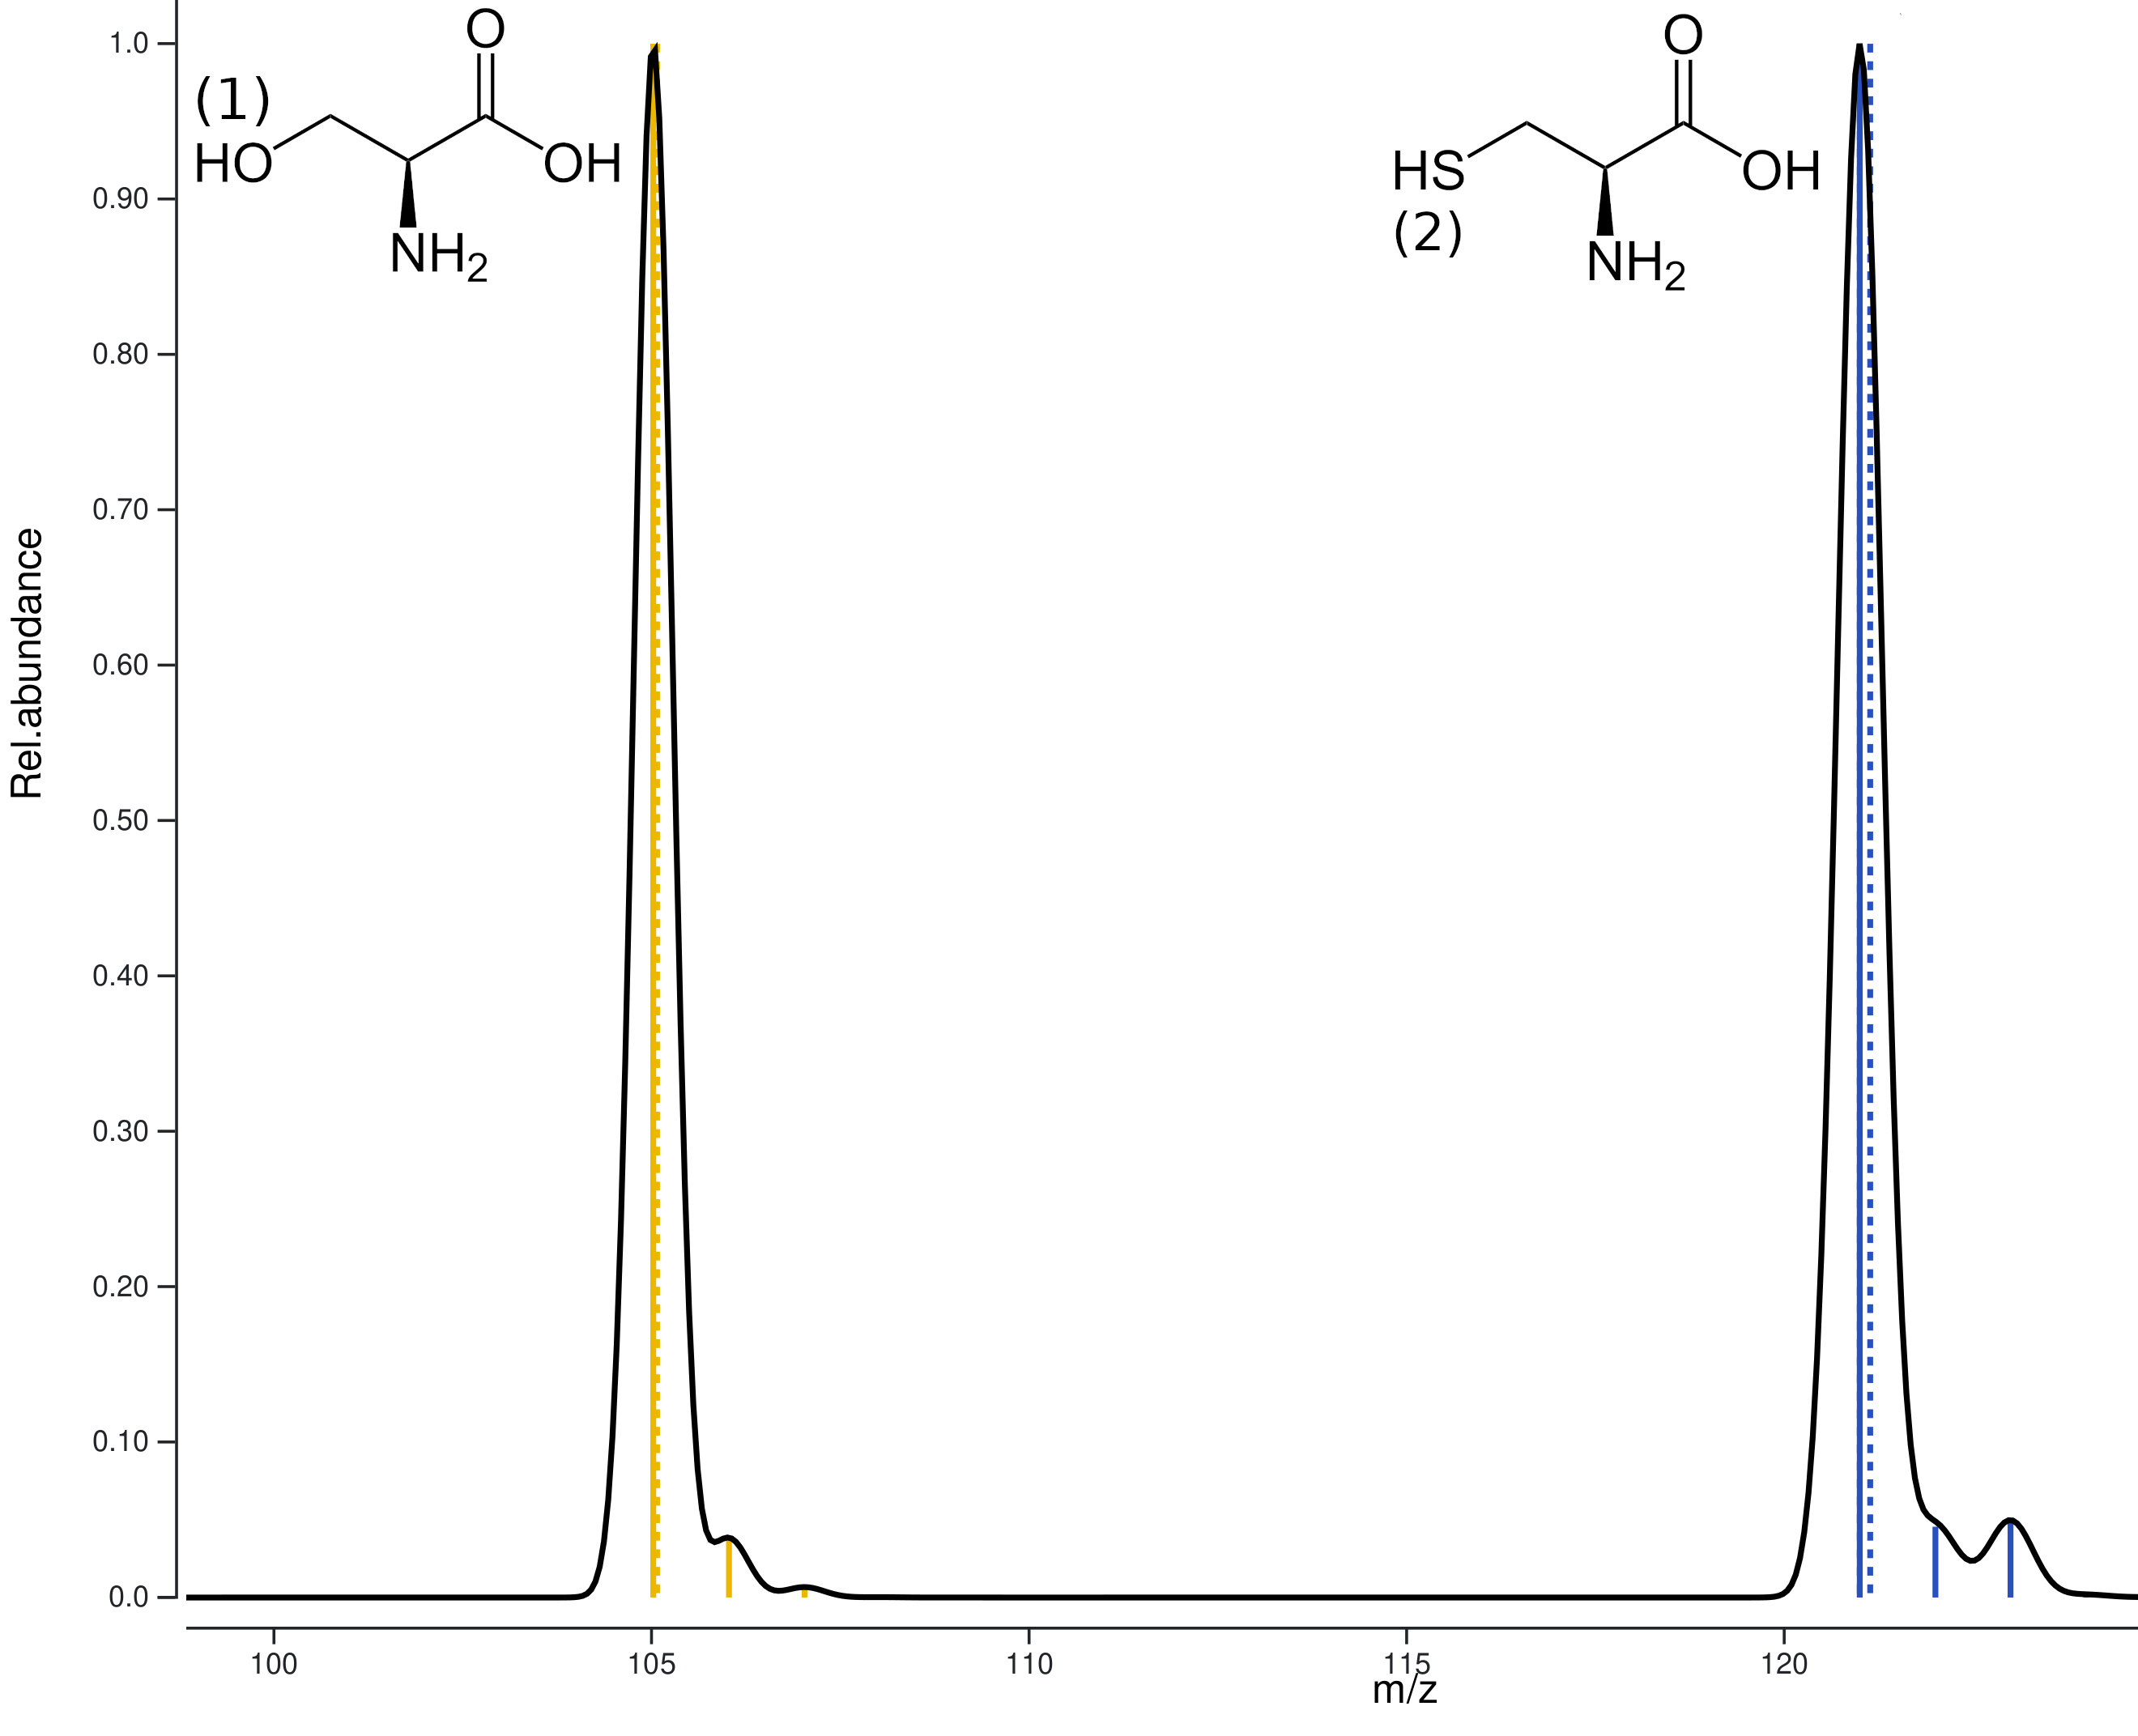
\includegraphics[width=0.75\textwidth]{./Resources/Simulated_Mass_Spectrum.png}
   \centering
   \caption{Computergeneriertes Massenspektrum von der Aminosäure \emph{Serin} (1) und \emph{Cystesin} (2). Peak von \emph{Serin} liegt bei 105; bei \emph{Systesin} um 121. y: relative Häufigkeit}
\end{figure}

Die Maxima werden \gerquot{Peaks} genannt und sind für eine Aminosäure an charakteristischer Position auf der $ x $-Achse. Obwohl sich die beiden Aminosäuren in der Abbildung \ref{fig:Sim_Mass_Spec} nur durch ein Atom unterscheiden (das linke Sauerstoffatom wurde durch ein Schwefelatom ersetzt) sind deren Massenspektren auf der $ x $-Achse weit voneinander entfernt und machen die beiden Aminosäuren dadurch sicher unterscheidbar.\\

Bei einzelnen Aminosäuren funktioniert die MS zuverlässig; bei Peptiden allerdings steht man vor dem Problem, dass das Massenspektrum unübersichtlicher wird und auch Peaks, die von Hintergrundrauschen stammen, schwerer herausgefiltert werden können. Abhilfe schafft hier die Tandem-Massenspektrometrie.

\subsection{Tandem-Massenspektrometrie (MS/MS)}\label{ss:Tandem_MS}
Bei der Tandem-Massenspektrometrie (MS/MS oder MS2) werden zwei MS Vorgänge hintereinander mit einer Probe durchgeführt. Die erste MS dient dazu Ionen aus einem bestimmten \massCharge Bereich auswählbar zu machen. Es entspricht also quasi einer Form der Filterung.

Vor der 2. MS werden die ausgewählten Reste einer Fragmentierung unterzogen. Bei einer Fragmentierung führt man Energie zu mit dem Ziel, dass die Ionen zerfallen und sog. Fragment-Ionen bilden. Diese Fragment-Ionen werden dann auf dem Massenspektrum nach der 2. MS sichtbar gemacht.

Fragment-Ionen sind kleiner als die ursprünglichen Ionen. So kann die 2. MS mit einer höheren Selektivität durchgeführt werden, welches Peaks durch Hintergrundrauschen verringert. Auch lassen sich Ionen besser identifizieren, die ein sehr ähnliches \massCharge-Verhältnis besitzen. Nach der 2. MS liegt eine Fülle an Fragment-Ionen-Peaks vor, aus denen sich die ursprünglichen Strukturinformationen ableiten lassen, da Ionen in spezifische Fragmente zerfallen \cite{Gross2013}. Zusammengefasst kann man sagen, dass das MS/MS Verfahren Ergebnisse höherer Güte erzeugt im Vergleich zur einfachen MS.

\section{De-Novo-Peptidsequenzierung mit \emph{pNovo+}}\label{s:pNovoPlusSeq}
Die \emph{pNovo+} Methode ist eine \gls{gls:DeNovo}, die mit einem \gls{gls:SpecGraph}en für die Auswertung der MS2-Spektren arbeitet und eine Erweiterung des \emph{pNovo} Verfahren darstellt \cite{pNovo}. Der Hauptansatz ist, dass zwei MS/MS Durchläufe mit jeweils verschiedenen Fragmentierungsmethoden\footnote{\emph{pNovo+} verwendet die higher energy
collisional dissociation (HCD) und die electron transfer dissociation (ETD) Fragmentierungsmethoden.} durchgeführt werden. Durch die Wahl einer anderen Fragmentierungsmethode ändert sich auch das MS2-Spektrum. Wenn nun Fragmentierungsmethoden verwendet werden, die möglichst komplementäre Spektren erzeugen, dann lässt sich durch das Zusammenführen der beiden MS2-Spektren die Qualität der Ergebnisse verbessern. Zum Beispiel lassen sich dadurch viele Peaks, die vom Hintergrundrauschen stammen, entfernen.

Für die Ermittlung der Sequenz eines Peptides wird zunächst ein Spektrums-Graph gebildet \dashAndSpace in Form eines DAG (directed acyclic graph). In diesem Graphen wird dann der längste Pfad bei gegebenen Start- und Endknoten berechnet. Die Reihenfolge der Knoten, die im längsten Pfad durchlaufen werden, stellt dann die Peptidsequenz dar.

\subsection{Vorverarbeitung der MS2-Spektren}\label{ss:Vorverarbeitung}
Bevor aus den MS2-Spektren der Spektrums-Graph gebildet werden kann, müssen die Daten vorverarbeitet werden. Für die Auswertung ist es von entscheidener Bedeutung, dass möglichst wenig Peaks verwendet werden, die vom Hintergrundrauschen stammen. Im weiteren Verlauf werden an einem exemplarischen MS2-Spektrum die Verarbeitungsschritte dargestellt.\\

Der erste Schritt ist das Verwenden des natürlichen Logarithmus der Intensitäten. Die Idee dabei ist, dass Hintergrundrauschen nicht überpriorisiert wird.

\begin{figure}[H]
   \centering
   \begin{minipage}[t]{.45\linewidth}
      \centering
      \begin{tikzpicture}[scale=\tikzScale, baseline=(current bounding box.center)]
         \draw [<->,thick] (0,\yAxisHeight) node (yaxis) [above] {\yAxisUnit}
         |- (\xAxisLength,0) node (xaxis) [right] {\xAxisUnit};
\draw[thick] (0.2, 0.0) -- (0.2, 2.3);
\draw[thick] (0.382, 0.0) -- (0.382, 1.7);
\draw[thick] (0.476, 0.0) -- (0.476, 2.7);
\draw[thick] (0.456, 0.0) -- (0.456, 1.8);
\draw[thick] (0.6859999999999999, 0.0) -- (0.6859999999999999, 2.7);
\draw[thick] (0.6839999999999999, 0.0) -- (0.6839999999999999, 1.8);
\draw[thick] (0.752, 0.0) -- (0.752, 1.1);
\draw[thick] (0.8200000000000001, 0.0) -- (0.8200000000000001, 2.2);
\draw[thick] (1.076, 0.0) -- (1.076, 1.5);
\draw[thick] (1.16, 0.0) -- (1.16, 1.9);
\draw[thick] (1.2120000000000002, 0.0) -- (1.2120000000000002, 2.0);
\draw[thick] (1.28, 0.0) -- (1.28, 1.9);
\draw[thick] (1.452, 0.0) -- (1.452, 1.3);
\draw[thick] (1.426, 0.0) -- (1.426, 1.9);
\draw[thick] (1.548, 0.0) -- (1.548, 1.9);
\draw[thick] (1.6740000000000002, 0.0) -- (1.6740000000000002, 1.5);
\draw[thick] (1.788, 0.0) -- (1.788, 2.5);
\draw[thick] (1.856, 0.0) -- (1.856, 2.3);
\draw[thick] (2.036, 0.0) -- (2.036, 1.7);
\draw[thick] (2.142, 0.0) -- (2.142, 1.6);
\draw[thick] (2.2520000000000002, 0.0) -- (2.2520000000000002, 2.0);
\draw[thick] (2.386, 0.0) -- (2.386, 1.6);
\draw[thick] (2.488, 0.0) -- (2.488, 2.9);
\draw[thick] (2.4739999999999998, 0.0) -- (2.4739999999999998, 2.7);
\draw[thick] (2.504, 0.0) -- (2.504, 2.0);
\draw[thick] (2.682, 0.0) -- (2.682, 2.0);
\draw[thick] (2.702, 0.0) -- (2.702, 2.5);
\draw[thick] (2.9259999999999997, 0.0) -- (2.9259999999999997, 2.8);
\draw[thick] (3.024, 0.0) -- (3.024, 2.4);
\draw[thick] (3.096, 0.0) -- (3.096, 1.8);
\draw[thick] (3.244, 0.0) -- (3.244, 2.6);
\draw[thick] (3.362, 0.0) -- (3.362, 1.9);
\draw[thick] (3.46, 0.0) -- (3.46, 2.3);
\draw[thick] (3.516, 0.0) -- (3.516, 1.1);
\draw[thick] (3.584, 0.0) -- (3.584, 1.8);
\draw[thick] (3.652, 0.0) -- (3.652, 2.0);
\draw[thick] (3.838, 0.0) -- (3.838, 1.5);
\draw[thick] (3.8819999999999997, 0.0) -- (3.8819999999999997, 2.6);
\draw[thick] (4.088, 0.0) -- (4.088, 2.6);
\draw[thick] (4.046, 0.0) -- (4.046, 1.1);
\draw[thick] (4.167999999999999, 0.0) -- (4.167999999999999, 2.0);
\draw[thick] (4.266, 0.0) -- (4.266, 2.4);
\draw[thick] (4.38, 0.0) -- (4.38, 1.1);
\draw[thick] (4.456, 0.0) -- (4.456, 2.2);
\draw[thick] (4.644, 0.0) -- (4.644, 2.6);
\draw[thick] (4.675999999999999, 0.0) -- (4.675999999999999, 2.5);
\draw[thick] (4.898000000000001, 0.0) -- (4.898000000000001, 1.2);
   \end{tikzpicture}%
   \end{minipage}%
   \textbf{$\rightarrow$} 
   \begin{minipage}[t]{.45\linewidth}
      \centering
      \begin{tikzpicture}[scale=\tikzScale, baseline=(current bounding box.center)]
      \draw [<->,thick] (0,\yAxisHeight) node (yaxis) [above] {\yAxisUnit}
      |- (\xAxisLength,0) node (xaxis) [right] {\xAxisUnit};
\draw[thick] (0.2, 0.0) -- (0.2, {ln(2.3)});
\draw[thick] (0.382, 0.0) -- (0.382, {ln(1.7)});
\draw[thick] (0.476, 0.0) -- (0.476, {ln(2.7)});
\draw[thick] (0.456, 0.0) -- (0.456, {ln(1.8)});
\draw[thick] (0.6859999999999999, 0.0) -- (0.6859999999999999, {ln(2.7)});
\draw[thick] (0.6839999999999999, 0.0) -- (0.6839999999999999, {ln(1.8)});
\draw[thick] (0.752, 0.0) -- (0.752, {ln(1.1)});
\draw[thick] (0.8200000000000001, 0.0) -- (0.8200000000000001, {ln(2.2)});
\draw[thick] (1.076, 0.0) -- (1.076, {ln(1.5)});
\draw[thick] (1.16, 0.0) -- (1.16, {ln(1.9)});
\draw[thick] (1.2120000000000002, 0.0) -- (1.2120000000000002, {ln(2.0)});
\draw[thick] (1.28, 0.0) -- (1.28, {ln(1.9)});
\draw[thick] (1.452, 0.0) -- (1.452, {ln(1.3)});
\draw[thick] (1.426, 0.0) -- (1.426, {ln(1.9)});
\draw[thick] (1.548, 0.0) -- (1.548, {ln(1.9)});
\draw[thick] (1.6740000000000002, 0.0) -- (1.6740000000000002, {ln(1.5)});
\draw[thick] (1.788, 0.0) -- (1.788, {ln(2.5)});
\draw[thick] (1.856, 0.0) -- (1.856, {ln(2.3)});
\draw[thick] (2.036, 0.0) -- (2.036, {ln(1.7)});
\draw[thick] (2.142, 0.0) -- (2.142, {ln(1.6)});
\draw[thick] (2.2520000000000002, 0.0) -- (2.2520000000000002, {ln(2.0)});
\draw[thick] (2.386, 0.0) -- (2.386, {ln(1.6)});
\draw[thick] (2.488, 0.0) -- (2.488, {ln(2.9)});
\draw[thick] (2.4739999999999998, 0.0) -- (2.4739999999999998, {ln(2.7)});
\draw[thick] (2.504, 0.0) -- (2.504, {ln(2.0)});
\draw[thick] (2.682, 0.0) -- (2.682, {ln(2.0)});
\draw[thick] (2.702, 0.0) -- (2.702, {ln(2.5)});
\draw[thick] (2.9259999999999997, 0.0) -- (2.9259999999999997, {ln(2.8)});
\draw[thick] (3.024, 0.0) -- (3.024, {ln(2.4)});
\draw[thick] (3.096, 0.0) -- (3.096, {ln(1.8)});
\draw[thick] (3.244, 0.0) -- (3.244, {ln(2.6)});
\draw[thick] (3.362, 0.0) -- (3.362, {ln(1.9)});
\draw[thick] (3.46, 0.0) -- (3.46, {ln(2.3)});
\draw[thick] (3.516, 0.0) -- (3.516, {ln(1.1)});
\draw[thick] (3.584, 0.0) -- (3.584, {ln(1.8)});
\draw[thick] (3.652, 0.0) -- (3.652, {ln(2.0)});
\draw[thick] (3.838, 0.0) -- (3.838, {ln(1.5)});
\draw[thick] (3.8819999999999997, 0.0) -- (3.8819999999999997, {ln(2.6)});
\draw[thick] (4.088, 0.0) -- (4.088, {ln(2.6)});
\draw[thick] (4.046, 0.0) -- (4.046, {ln(1.1)});
\draw[thick] (4.167999999999999, 0.0) -- (4.167999999999999, {ln(2.0)});
\draw[thick] (4.266, 0.0) -- (4.266, {ln(2.4)});
\draw[thick] (4.38, 0.0) -- (4.38, {ln(1.1)});
\draw[thick] (4.456, 0.0) -- (4.456, {ln(2.2)});
\draw[thick] (4.644, 0.0) -- (4.644, {ln(2.6)});
\draw[thick] (4.675999999999999, 0.0) -- (4.675999999999999, {ln(2.5)});
\draw[thick] (4.898000000000001, 0.0) -- (4.898000000000001, {ln(1.2)});
      \end{tikzpicture}
      \end{minipage}
      \caption{Anwendung des $ ln $ auf einem exemplarischen MS2-Spektrum.}
\end{figure}

Für das Verständnis des nächsten Schrittes muss man sich in Erinnerung rufen, dass eine gleiche Aminosäure keineswegs immer die gleiche Masse hat. Durch Isotope existiert eine gewisse \gerquot{Massenbandbreite} für ein und dieselbe Aminosäure. MS Systeme sind heute so genau, dass sie diese Differenzen erkennen. Dies hat den ungewollten Effekt, dass mehrere Peaks zu einer Aminosäure gehören können \cite{IsotopicDistributionMS}. Gleichzeitig können die \gerquot{Massenbandbreiten} zweier Aminosäuren sich überschneiden, sodass im ungünstigen Fall zwei Peaks kaum unterscheidbar nebeneinander liegen.\\

Eine Möglichkeit mit dieser Problematik umzugehen ist die Verwendung der monoisotopischen Masse. Die monoisotopische Masse ist die \gerquot{[...] exact mass of the most abundant naturally occurring stable isotope determined relative to the mass of 12 C, which is assigned the exact value of 12.0000.} \cite{MonoisotopicMass}. Ohne dabei jetzt tiefer ins Detail zu gehen kann man sagen, dass alle Peaks, deren Intensität mit einer möglichen monoisotopischen Masse übereinstimmen, auf jeden Fall einer Aminosäure entsprechen und (höchstwahrscheinlich)\footnote{Natürlich ist es möglich, dass das Rauschen zufällig einer monoisotopischen Masse entspricht. Die Wahrscheinlichkeit dafür ist allerdings sehr gering.} kein Hintergrundrauschen sind \cite{MassDefectMS}. Diese Peaks bekommen eine sogennante \emph{charge state}.\\

Der Algorithmus verwendet die \emph{charge state} Peaks als Ausganspunkte für weitere Berechnungen. Wenn die \massCharge Differenz zu einem anderen Peak einem Peptidfragment entspricht, dann stammt dieser Peak höchstwahrscheinlich von einem Fragment. Insgesamt werden damit die relevanten Peptidfragmente herausgeholt. Abbildung \ref{MonoisotopicMassFiltering} zeigt das Ergebnis nach den beiden zuvor genannten Schritten.

\begin{figure}[H]\label{MonoisotopicMassFiltering}
   \centering
   \begin{minipage}[t]{.45\linewidth}
      \centering
      \begin{tikzpicture}[scale=\tikzScale, baseline=(current bounding box.center)]
         \draw [<->,thick] (0,\yAxisHeight) node (yaxis) [above] {\yAxisUnit}
         |- (\xAxisLength,0) node (xaxis) [right] {\xAxisUnit};
\draw[thick] (0.2, 0.0) -- (0.2, {ln(2.3)});
\draw[color=blue!85!,opacity=.55,thick] (0.382, 0.0) -- (0.382, {ln(1.7)});
\draw[color=blue!85!,opacity=.55,thick] (0.476, 0.0) -- (0.476, {ln(2.7)});
\draw[color=magenta,thick] (0.456, 0.0) -- (0.456, {ln(1.8)});
\draw[color=blue!85!,opacity=.55,thick] (0.6859999999999999, 0.0) -- (0.6859999999999999, {ln(2.7)});
\draw[color=blue!85!,opacity=.55,thick] (0.6839999999999999, 0.0) -- (0.6839999999999999, {ln(1.8)});
\draw[thick] (0.752, 0.0) -- (0.752, {ln(1.1)});
\draw[thick] (0.8200000000000001, 0.0) -- (0.8200000000000001, {ln(2.2)});
\draw[thick] (1.076, 0.0) -- (1.076, {ln(1.5)});
\draw[thick] (1.16, 0.0) -- (1.16, {ln(1.9)});
\draw[thick] (1.2120000000000002, 0.0) -- (1.2120000000000002, {ln(2.0)});
\draw[thick] (1.28, 0.0) -- (1.28, {ln(1.9)});
\draw[color=blue!85!,opacity=.55,thick] (1.452, 0.0) -- (1.452, {ln(1.3)});
\draw[color=blue!85!,opacity=.55,thick] (1.426, 0.0) -- (1.426, {ln(1.9)});
\draw[color=magenta,thick] (1.548, 0.0) -- (1.548, {ln(1.9)});
\draw[color=blue!85!,opacity=.55,thick] (1.6740000000000002, 0.0) -- (1.6740000000000002, {ln(1.5)});
\draw[color=blue!85!,opacity=.55,thick] (1.788, 0.0) -- (1.788, {ln(2.5)});
\draw[thick] (1.856, 0.0) -- (1.856, {ln(2.3)});
\draw[thick] (2.036, 0.0) -- (2.036, {ln(1.7)});
\draw[thick] (2.142, 0.0) -- (2.142, {ln(1.6)});
\draw[thick] (2.2520000000000002, 0.0) -- (2.2520000000000002, {ln(2.0)});
\draw[thick] (2.386, 0.0) -- (2.386, {ln(1.6)});
\draw[color=blue!85!,opacity=.55,thick] (2.488, 0.0) -- (2.488, {ln(2.9)});
\draw[thick] (2.4739999999999998, 0.0) -- (2.4739999999999998, {ln(2.7)});
\draw[color=blue!85!,opacity=.55,thick] (2.504, 0.0) -- (2.504, {ln(2.0)});
\draw[color=magenta,thick] (2.682, 0.0) -- (2.682, {ln(2.0)});
\draw[color=blue!85!,opacity=.55,thick] (2.702, 0.0) -- (2.702, {ln(2.5)});
\draw[thick] (2.9259999999999997, 0.0) -- (2.9259999999999997, {ln(2.8)});
\draw[thick] (3.024, 0.0) -- (3.024, {ln(2.4)});
\draw[thick] (3.096, 0.0) -- (3.096, {ln(1.8)});
\draw[thick] (3.244, 0.0) -- (3.244, {ln(2.6)});
\draw[thick] (3.362, 0.0) -- (3.362, {ln(1.9)});
\draw[color=blue!85!,opacity=.55,thick] (3.46, 0.0) -- (3.46, {ln(2.3)});
\draw[color=blue!85!,opacity=.55,thick] (3.516, 0.0) -- (3.516, {ln(1.1)});
\draw[color=blue!85!,opacity=.55,thick] (3.584, 0.0) -- (3.584, {ln(1.8)});
\draw[color=magenta,thick] (3.652, 0.0) -- (3.652, {ln(2.0)});
\draw[color=blue!85!,opacity=.55,thick] (3.838, 0.0) -- (3.838, {ln(1.5)});
\draw[color=blue!85!,opacity=.55,thick] (3.8819999999999997, 0.0) -- (3.8819999999999997, {ln(2.6)});
\draw[thick] (4.088, 0.0) -- (4.088, {ln(2.6)});
\draw[thick] (4.046, 0.0) -- (4.046, {ln(1.1)});
\draw[thick] (4.167999999999999, 0.0) -- (4.167999999999999, {ln(2.0)});
\draw[thick] (4.266, 0.0) -- (4.266, {ln(2.4)});
\draw[color=blue!85!,opacity=.55,thick] (4.38, 0.0) -- (4.38, {ln(1.1)});
\draw[color=blue!85!,opacity=.55,thick] (4.456, 0.0) -- (4.456, {ln(2.2)});
\draw[color=magenta,thick] (4.644, 0.0) -- (4.644, {ln(2.6)});
\draw[color=blue!85!,opacity=.55,thick] (4.675999999999999, 0.0) -- (4.675999999999999, {ln(2.5)});
\draw[color=blue!85!,opacity=.55,thick] (4.898000000000001, 0.0) -- (4.898000000000001, {ln(1.2)});
   \end{tikzpicture}%
   \end{minipage}%
   \textbf{$\rightarrow$} 
   \begin{minipage}[t]{.45\linewidth}
      \centering
      \begin{tikzpicture}[scale=\tikzScale, baseline=(current bounding box.center)]
      \draw [<->,thick] (0,\yAxisHeight) node (yaxis) [above] {\yAxisUnit}
      |- (\xAxisLength,0) node (xaxis) [right] {\xAxisUnit};
\draw[color=blue!85!,opacity=.55,thick] (0.382, 0.0) -- (0.382, {ln(1.7)});
\draw[color=blue!85!,opacity=.55,thick] (0.476, 0.0) -- (0.476, {ln(2.7)});
\draw[color=magenta,thick] (0.456, 0.0) -- (0.456, {ln(1.8)});
\draw[color=blue!85!,opacity=.55,thick] (0.6859999999999999, 0.0) -- (0.6859999999999999, {ln(2.7)});
\draw[color=blue!85!,opacity=.55,thick] (0.6839999999999999, 0.0) -- (0.6839999999999999, {ln(1.8)});
\draw[color=blue!85!,opacity=.55,thick] (1.452, 0.0) -- (1.452, {ln(1.3)});
\draw[color=blue!85!,opacity=.55,thick] (1.426, 0.0) -- (1.426, {ln(1.9)});
\draw[color=magenta,thick] (1.548, 0.0) -- (1.548, {ln(1.9)});
\draw[color=blue!85!,opacity=.55,thick] (1.6740000000000002, 0.0) -- (1.6740000000000002, {ln(1.5)});
\draw[color=blue!85!,opacity=.55,thick] (1.788, 0.0) -- (1.788, {ln(2.5)});
\draw[color=blue!85!,opacity=.55,thick] (2.488, 0.0) -- (2.488, {ln(2.9)});
\draw[color=blue!85!,opacity=.55,thick] (2.504, 0.0) -- (2.504, {ln(2.0)});
\draw[color=magenta,thick] (2.682, 0.0) -- (2.682, {ln(2.0)});
\draw[color=blue!85!,opacity=.55,thick] (2.702, 0.0) -- (2.702, {ln(2.5)});
\draw[color=blue!85!,opacity=.55,thick] (3.46, 0.0) -- (3.46, {ln(2.3)});
\draw[color=blue!85!,opacity=.55,thick] (3.516, 0.0) -- (3.516, {ln(1.1)});
\draw[color=blue!85!,opacity=.55,thick] (3.584, 0.0) -- (3.584, {ln(1.8)});
\draw[color=magenta,thick] (3.652, 0.0) -- (3.652, {ln(2.0)});
\draw[color=blue!85!,opacity=.55,thick] (3.838, 0.0) -- (3.838, {ln(1.5)});
\draw[color=blue!85!,opacity=.55,thick] (3.8819999999999997, 0.0) -- (3.8819999999999997, {ln(2.6)});
\draw[color=blue!85!,opacity=.55,thick] (4.38, 0.0) -- (4.38, {ln(1.1)});
\draw[color=blue!85!,opacity=.55,thick] (4.456, 0.0) -- (4.456, {ln(2.2)});
\draw[color=magenta,thick] (4.644, 0.0) -- (4.644, {ln(2.6)});
\draw[color=blue!85!,opacity=.55,thick] (4.675999999999999, 0.0) -- (4.675999999999999, {ln(2.5)});
\draw[color=blue!85!,opacity=.55,thick] (4.898000000000001, 0.0) -- (4.898000000000001, {ln(1.2)});
      \end{tikzpicture}
      \end{minipage}
      \caption{Entfernen von Peaks, die keiner monoisotopischen Masse entsprechen oder benachbart mit einer Differenz von einem Fragment-Ion sind.}
\end{figure}

Tatsächlich ist die Verarbeitung an dieser Stelle noch etwas komplexer. So existieren auch noch sogenannte \emph{isotopic cluster}\footnote{Definition eines \emph{isotopic cluster} nach IUPAC: \gerquot{Group of peaks representing ions of the same elemental composition, but different isotopic compositions.} \cite[1556]{IUPACDefinitions}}, die gesondert verarbeitet werden. Für das grundsätzliche Prinzip ist dieses Detail allerdings weniger relevant.\\

Im letzten Vorberarbeitungsschritt werden Peaks aus einem irrelevanten \massCharge Bereich entfernt und naheliegende Peaks werden zusammengefasst, indem der Mittelwert sowol des \massCharge Wertes als auch der der Intensität besimmt wird. Üblicherweise liegt der Bereich für das Zusammenfassen bei $ +- 20 ppm $.

\begin{figure}[H]
   \centering
   \begin{minipage}[t]{.45\linewidth}
      \centering
      \begin{tikzpicture}[scale=\tikzScale, baseline=(current bounding box.center)]
         \draw [<->,thick] (0,\yAxisHeight) node (yaxis) [above] {\yAxisUnit}
         |- (\xAxisLength,0) node (xaxis) [right] {\xAxisUnit};
\draw[thick] (0.382, 0.0) -- (0.382, {ln(1.7)});
\draw[thick] (0.476, 0.0) -- (0.476, {ln(2.7)});
\draw[thick] (0.456, 0.0) -- (0.456, {ln(1.8)});
\draw[thick] (0.6859999999999999, 0.0) -- (0.6859999999999999, {ln(2.7)});
\draw[thick] (0.6839999999999999, 0.0) -- (0.6839999999999999, {ln(1.8)});
\draw[color=red,thick] (1.452, 0.0) -- (1.452, {ln(1.3)});
\draw[color=red,thick] (1.426, 0.0) -- (1.426, {ln(1.9)});
\draw[thick] (1.548, 0.0) -- (1.548, {ln(1.9)});
\draw[thick] (1.6740000000000002, 0.0) -- (1.6740000000000002, {ln(1.5)});
\draw[thick] (1.788, 0.0) -- (1.788, {ln(2.5)});
\draw[color=red,thick] (2.488, 0.0) -- (2.488, {ln(2.9)});
\draw[color=red,thick] (2.504, 0.0) -- (2.504, {ln(2.0)});
\draw[color=red,thick] (2.682, 0.0) -- (2.682, {ln(2.0)});
\draw[color=red,thick] (2.702, 0.0) -- (2.702, {ln(2.5)});
\draw[thick] (3.46, 0.0) -- (3.46, {ln(2.3)});
\draw[thick] (3.516, 0.0) -- (3.516, {ln(1.1)});
\draw[thick] (3.584, 0.0) -- (3.584, {ln(1.8)});
\draw[thick] (3.652, 0.0) -- (3.652, {ln(2.0)});
\draw[color=red,thick] (3.838, 0.0) -- (3.838, {ln(1.5)});
\draw[color=red,thick] (3.8819999999999997, 0.0) -- (3.8819999999999997, {ln(2.6)});
\draw[thick] (4.38, 0.0) -- (4.38, {ln(1.1)});
\draw[thick] (4.456, 0.0) -- (4.456, {ln(2.2)});
\draw[thick] (4.644, 0.0) -- (4.644, {ln(2.6)});
\draw[thick] (4.675999999999999, 0.0) -- (4.675999999999999, {ln(2.5)});
\draw[thick] (4.898000000000001, 0.0) -- (4.898000000000001, {ln(1.2)});

\fill[red!25!,opacity=.25] (0,0) rectangle (1,\yAxisHeight-\axisColorOffset);
         \fill[red!25!,opacity=.25] (\xAxisLength-1,0) rectangle (\xAxisLength-\axisColorOffset,\yAxisHeight-\axisColorOffset);
         \fill[green!25!,opacity=.25] (1,0) rectangle (\xAxisLength-1,\yAxisHeight-\axisColorOffset);
   \end{tikzpicture}%
   \end{minipage}%
   \textbf{$\rightarrow$} 
   \begin{minipage}[t]{.45\linewidth}
      \centering
      \begin{tikzpicture}[scale=\tikzScale, baseline=(current bounding box.center)]
      \draw [<->,thick] (0,\yAxisHeight) node (yaxis) [above] {\yAxisUnit}
      |- (\xAxisLength,0) node (xaxis) [right] {\xAxisUnit};
%\draw[color=red,thick] (1.452, 0.0) -- (1.452, {ln(1.3)});
%\draw[color=red,thick] (1.426, 0.0) -- (1.426, {ln(1.9)});
\draw[color=red,ultra thick] ({(1.452+1.426)/2}, 0.0) -- ({(1.452+1.426)/2}, {(ln(1.3)+ln(1.9))/2});

\draw[thick] (1.548, 0.0) -- (1.548, {ln(1.9)});
\draw[thick] (1.6740000000000002, 0.0) -- (1.6740000000000002, {ln(1.5)});
\draw[thick] (1.788, 0.0) -- (1.788, {ln(2.5)});

%\draw[color=red,thick] (2.488, 0.0) -- (2.488, {ln(2.9)});
%\draw[color=red,thick] (2.504, 0.0) -- (2.504, {ln(2.0)});
\draw[color=red,ultra thick] ({(2.488+2.504)/2}, 0.0) -- ({(2.488+2.504)/2}, {(ln(2.9)+ln(2.0))/2});

%\draw[color=red,thick] (2.682, 0.0) -- (2.682, {ln(2.0)});
%\draw[color=red,thick] (2.702, 0.0) -- (2.702, {ln(2.5)});
\draw[color=red,ultra thick] ({(2.682+2.702)/2}, 0.0) -- ({(2.682+2.702)/2}, {(ln(2.0+ln(2.5))/2});

\draw[thick] (3.46, 0.0) -- (3.46, {ln(2.3)});
\draw[thick] (3.516, 0.0) -- (3.516, {ln(1.1)});
\draw[thick] (3.584, 0.0) -- (3.584, {ln(1.8)});
\draw[thick] (3.652, 0.0) -- (3.652, {ln(2.0)});

%\draw[color=red,thick] (3.838, 0.0) -- (3.838, {ln(1.5)});
%\draw[color=red,thick] (3.8819999999999997, 0.0) -- (3.8819999999999997,{ln(2.6)});
\draw[color=red,ultra thick] ({(3.838+3.8819999999999997)/2}, 0.0) -- ({(3.838+3.8819999999999997)/2}, {(ln(1.5)+ln(2.6))/2});

\fill[red!25!,opacity=.25] (0,0) rectangle (1,\yAxisHeight-\axisColorOffset);
         \fill[red!25!,opacity=.25] (\xAxisLength-1,0) rectangle (\xAxisLength-\axisColorOffset,\yAxisHeight-\axisColorOffset);
         \fill[green!25!,opacity=.25] (1,0) rectangle (\xAxisLength-1,\yAxisHeight-\axisColorOffset);
      \end{tikzpicture}
      \end{minipage}
      \caption{Entfernen von Peaks aus einem irrelevanten \massCharge Bereich und zusammenfassen naheliegender Peaks. Rot markierte Peaks sind jene, die zusammengefasst werden.}
\end{figure}

\subsection{Bildung eines Spektrums-Graphen}\label{ss:BildungSpekGraph}
Der Spektrums-Graph wird aus einem vorverarbeiteten MS2-Spektrum (siehe Kapitel: \ref{ss:Vorverarbeitung}) gebildet. Im initialen Zustand werden die Peaks als Knoten interpretiert. Dazu kommt ein Start- und Endknoten. Jedem Knoten wird eine Masse zugeordet; im initialen Zustand bekommt der Startknoten die Masse 0 und der Endknoten die Masse des vorherigen Knotens minus der Masse des Wassers ($ 18,02 $). Die Masse der übrigen Knoten entsprechen ihren jeweils korrespondierenden \massCharge Wert. Die gerichteten Kanten werden zwischen einem Knotenpaar hinzugefügt, wenn die Differenz deren Masse gleich ist mit der Masse von ein oder zwei Aminosäuren.

\subsection{Identifikation der Aminosäuresequenz}
Der gebildete DAG kann mit klassischen Algorithmen, die den längsten Pfad suchen, durchlaufen werden. Bezogen auf die Graphentheorie entspricht die Ermittlung der Aminosäurensequenz dem Suchen eines bestimmten Pfades \dashAndSpace und nicht nach irgendeinem Pfad. Daher muss der Algorithmus mittels einer Breitensuche arbeiten, um alle möglichen Pfade zu bestimmen.

In aller Regel wird es mehrere Pfade geben. Bestimmte Sequenzen sind wahrscheinlicher als andere. So sind Pfade mit Kanten, die wegen der Massendifferenz von genau einer Aminosäure gebildet wurden, wahrscheinlicher \cite{pNovoPlus}. Alle Pfade bekommen mittels einer Scoring-Funktion einen Wert zugewiesen. Der Pfad mit dem höchsten Scoring-Wert ist wahrscheinlich das richtige Ergebnis. Die Scoring-Funktion berücksichtigt unter anderem wie viele Fragmente, die einer bestimmten Aminosäure zugeordet werden können, im MS2-Spektrum vorhanden sind \cite{pNovo}. Die Sequenz mit dem höchsten Scoring-Wert ist das Endergebnis.

\section{De-Novo-Peptidsequenzierung mit \emph{Open-pNovo}}\label{s:OpenpNovoSeq}
Bei Proteinen können posttranslationale Proteinmodifikationen (PTM) auftreten. PTMs sind Ereignisse, bei denen sich Änderungen im Protein einstellen \cite{Mann2003}; teilweise sind die Änderungen von einer Zelle erwünscht \dashAndSpace teilweise stammen sie aber auch zum Beispiel von unerwünschten Wechselwirkungen nebeneinanderliegenden Aminosäuren. Ein Teil dieser PTMs führen zu einer Änderung der Aminosäuresequenz. Dies ist für die \gls{gls:DeNovo} nicht weiter problematisch, da sowieso ohne eine Datenbank gearbeitet wird, sodass solche PTMs nicht einmal auffallen würden. Andere PTMs hingegen haben die Auswirkung, dass Stoffe gebildet werden, die nicht mehr zu der Gruppe der proteinogenen Aminosäuren gehören. Proteinogene Aminosäuren sind jene Aminosäuren, die für den Bau von Proteinen verwendet werden. Der Effekt ist also, dass Stoffe (oder deren Fragmente) bei einem Massenspektrum angezeigt werden, die kein Teil eines Peptids sein können. Bei der Sequenzierung von Peptidfragmenten muss dies daher berücksichtigt werden.
Wenn im weiteren Verlauf von PTMs gesprochen wird, dann sind solche gemeint, die für die \gls{gls:DeNovo} relevant sind.

Open-pNovo ist ein \gls{gls:DeNovo}sverfahren, welches auf pNovo+ Tool aufbaut und versucht die Problematik mit den PTMs zu lösen.

\subsection{PTMs im konstruierten DAG}
Die Konvertierung eines MS2-Spektrums läuft bis zum DAG analog ab wie in den Kapiteln \ref{ss:Vorverarbeitung} und \ref{ss:BildungSpekGraph} für pNovo+. Der Unterschied ist nun, dass es zwei Arten von Kanten gibt:

\begin{itemize}
   \item \gerquot{Normale} Kanten: Kanten, die gebildet werden, wie es bereits für \emph{pNovo+} gezeigt wurde. 
   \item \gerquot{Modifizierte} Kanten: Kanten, die zum Grahpen hinzugefügt werden, wenn die Massendifferenz zweier Knoten der Masse einer Aminosäure plus der Masse einer möglichen PTM-Änderung entspricht. 
\end{itemize}

Eine Liste aller PTMs in der Datenbank Unimod (sowohl relevante als auch nicht relevante) beinhaltet aktuell 1510 Einträge\footnote{Siehe: \url{https://www.ebi.ac.uk/ols/ontologies/unimod}} (Stand: 18.04.2022). Für die modifizierten Kanten gibt es insgesamt $ 1510 * 20 = 30200 $ mögliche Differenzen, wobei viele davon nicht relevante PTMs sind. Zum Vergleich: bei den normalen Kanten gibt es $ 20^2 = 400 $ mögliche Differenzen.

Die hohe Anzahl an Differenzen für modifizierte Kanten hat die Konsequenz, dass viele Knoten zufällig verbunden werden und dass dadurch die Genauigkeit der Ergebnisse abnimmt. Dieses Problem kann man durch eine geringere Liste an möglichen PTMs abfedern, allerdings mit einem Verlust  der Genauigkeit auf Seiten der PTMs. Es ist hier also eine Abwägung.

\subsection{Evaluierung von Open-pNovo}
Open-pNovo wurde sowohl auf drei realen als auch auf drei generierten Testdaten getestet. Tabelle \ref{tab:OpenPNovoResults} zeigt die Ergebnisse im Vergleich zu pNovo+ und zwei anderen Algorithmen. Die Datensätze enthielten die am häufigsten vorkommenden PTMs.

\begin{table}[H]
    \centering
    \begin{tabular}{l|c|c|c|c}
        \toprule
        \textbf{Testdatensätze} & \textbf{Open-pNovo+} & \textbf{pNovo+} & \textbf{PEAKS} & \textbf{Novor} \\
        \midrule
        Real (20259) & $76,3 \%$ & $68,5 \%$ & $65,8 \%$ & $39,9 \%$ \\
        Generiert (17877) & $77,8 \%$ & $0,6 \%$ & $0,5 \%$ & $0,2 \%$ \\
        \bottomrule
    \end{tabular}
    \newline
    \caption{Vergleich der durchschnittlichen richtigen \gls{gls:DeNovo} Peptidsequenzierungen von Open-pNovo und anderen Algorithmen \cite[650]{OpenPNovo}.}
    \label{tab:OpenPNovoResults}
\end{table}

Die enorm schlechten Ergebnisse der anderen Algorithmen bei den generierten Testdaten ist ein Nebeneffekt des Ziels bei der Testdatengenerierung. Denn diese wurden so ausgelegt, um die Grenzen von Open-pNovo+ zu ermitteln \cite[649]{OpenPNovo}. Eine Aussagekraft haben diese Ergebnisse also nicht. Allerdings auch bei realen Testdaten zeigt sich Open-pNovo als voll konkurrenzfähig gegenüber den anderen Algorithmen.

Noch besser zeigt sich Open-pNovo, wenn der Recall Wert betrachtet wird \dashAndSpace also die Anzahl an verschiedenen PSMs, die erkannt wurden. In diesem Fall ist der Abstand zu den anderen Algorithmen deutlich größer geworden.

\begin{table}[H]
    \centering
    \begin{tabular}{l|c|c|c|c}
        \toprule
        \textbf{Testdatensätze} & \textbf{Open-pNovo+} & \textbf{pNovo+} & \textbf{PEAKS} & \textbf{Novor} \\
        \midrule
        Real (5034) & $61,6 \%$ & $31,3 \%$ & $32,0 \%$ & $13,7 \%$ \\
        \bottomrule
    \end{tabular}
    \newline
    \caption{Vergleich der durchschnittlichen Recall Werte einer \gls{gls:DeNovo} Peptidsequenzierungen von Open-pNovo und anderen Algorithmen \cite[650]{OpenPNovo}.}
    \label{tab:OpenPNovoResultsRecall}
\end{table}

\subsection{Zusammenfassung}


% Die \gls{gls:DeNovo} nutzt die sogenannte \gls{gls:TMassSpek} für die Bestimmung der Peptidsequenz. Dabei wird die physikalische Eigenschaft ausgenutzt, dass jedes Atom bzw. jedes Molekül \dashAndSpace wenn es einer \gls{gls:Ionisation} unterzogen wurde \dashAndSpace ein charakteristisches \gls{gls:MassSpek} besitzt. Das \gls{gls:MassSpek} stellt also eine Art \gerquot{Fingerabdruck} eines Moleküls dar und macht dieses ermittelbar.

% U.U. eine Beispielgrafik eines Massenspektrums hinzufuegen ...

\subsubsection{\glsentrytext{gls:TMassSpek} bei größeren Molekülen}
Bei größeren Molekülen (wie einem Protein) führt die \gls{gls:Ionisation} dazu, dass das Molekül in kleinere spezifische Ionen zerfällt (sog. Fragmentierung). Die Fragmentierungsinformationen einer \gls{gls:DeNovo} sind meist unvollständig, da fehlende Daten bei einem Fragmentierungsschritt die Güte des Endergebnisses negativ beeinflusst. Dies wird insbesondere dann ein Problem, wenn unbekannte Änderungen in einer Peptidsequenz vorhanden sind.

Um dieses Problem zu verringern können unterschiedliche Techniken parallel eingesetzt werden, welche verschiedene Fragmente erzeugen und daher auch verschiedenartige \glspl{gls:MassSpek} zur Folge haben.\footnote{Konkret: Es wird sowohl das \gls{acr:HCD} als auch das \gls{acr:ETD} Verfahren angewendet.}

\subsection{Datenaufbereitung}
Typischerweise betrachtet man die sog. \gerquot{\glspl{gls:Peak}} in den \glspl{gls:MassSpek}. Jeder \gls{gls:Peak} stellt ein unterschiedliches Ion dar. Dazu kommen Messungenauigkeiten sowie Hintergrundrauschen. Durch die hohe Anzahl an möglichen Ionen kann nicht ohne weiteres differenziert werden, welcher der \glspl{gls:Peak} von welchen Ionen erzeugt wurden und welche nicht.

% Frage an Dominik: Ist hier eine einfache Auflistung an Techniken für die Datenaufbereitung besser?
Der Algorithmus für die Datenaufbereitung berechnet den natürlichen Logarithmus von den Intensitäten der \glspl{gls:Peak}, um Hintergrundrauschen und Messungenauigkeiten nicht überzupriorisieren. Zusätzlich dazu werden \glspl{gls:Peak}, die in einem Toleranzbereich nebeneinander liegen, zusammengefasst. Am Ende werden die \glspl{gls:Peak} entfernt, bei denen bekannt ist, dass es sich nicht um relevante Ionen handeln kann. (z.B. \glspl{gls:Peak} von Isotopen)

\begin{figure}[H]
   \centering
   \begin{minipage}[t]{.4\linewidth}
      \centering
      \begin{tikzpicture}[scale=\tikzScale, baseline=(current bounding box.center)]
         \draw [<->,thick] (0,2.75) node (yaxis) [above] {\yAxisUnit}
         |- (3,0) node (xaxis) [right] {\xAxisUnit};

         \draw[thick] (0.2,0) -- (0.2,1.1);
         \draw[thick] (0.3,0) -- (0.3,1.6);
         \draw[thick] (0.6,0) -- (0.6,1.7);
         \draw[thick] (0.8,0) -- (0.8,1.2);
         \draw[thick] (1.0,0) -- (1.0,1.1);

         \draw[color=red,thick] (1.2,0) -- (1.2,2.65);
         \draw[thick] (1.4,0) -- (1.4,1.4);
         \draw[thick] (1.6,0) -- (1.6,1.2);
         \draw[thick] (1.8,0) -- (1.8,1.3);
         \draw[thick] (2.0,0) -- (2.0,1.8);

         \draw[thick] (1.1,0) -- (1.1,2.0);
         \draw[color=red,thick] (0.35,0) -- (0.35,2.25);
         \draw[thick] (1.9,0) -- (1.9,1.4);
         \draw[color=red,thick] (2.2,0) -- (2.2,2.6);
         \draw[thick] (2.5,0) -- (2.5,1.25);

         \draw[thick] (2.7,0) -- (2.7,1.1);
         \foreach \x in {1,...,6}
         {
            \draw[thick] (1.2+\x*0.05,0) -- (1.2+\x*0.05,1.0+\x*0.15);
         }
      \end{tikzpicture}%
      % \subcaption{Exemplarische Rohdaten}
   \end{minipage}%
   \textbf{$\rightarrow$}
   \begin{minipage}[t]{.4\linewidth}
      \centering
      \begin{tikzpicture}[scale=\tikzScale, baseline=(current bounding box.center)]
         \draw [<->,thick] (0,2.75) node (yaxis) [above] {\yAxisUnit}
         |- (3,0) node (xaxis) [right] {\xAxisUnit};

         \draw[thick] (0.2,0) -- (0.2,{ln(1.1)});
         \draw[thick] (0.3,0) -- (0.3,{ln(1.6)});
         \draw[thick] (0.6,0) -- (0.6,{ln(1.7)});
         \draw[thick] (0.8,0) -- (0.8,{ln(1.2)});
         \draw[thick] (1.0,0) -- (1.0,{ln(1.1)});

         \draw[color=red,thick] (1.2,0) -- (1.2,{ln(2.65)});
         \draw[thick] (1.4,0) -- (1.4,{ln(1.4)});
         \draw[thick] (1.6,0) -- (1.6,{ln(1.2)});
         \draw[thick] (1.8,0) -- (1.8,{ln(1.3)});
         \draw[thick] (2.0,0) -- (2.0,{ln(1.8)});

         \draw[thick] (1.1,0) -- (1.1,{ln(2.0)});
         \draw[color=red,thick] (0.35,0) -- (0.35,{ln(2.25)});
         \draw[thick] (1.9,0) -- (1.9,{ln(1.4)});
         \draw[color=red,thick] (2.2,0) -- (2.2,{ln(2.6)});
         \draw[thick] (2.5,0) -- (2.5,{ln(1.25)});

         \draw[thick] (2.7,0) -- (2.7,{ln(1.1)});
         \foreach \x in {1,...,6}
         {%
            \draw[thick] (1.2+\x*0.05,0) -- (1.2+\x*0.05,{ln(1.0+\x*0.15)});
         }
      \end{tikzpicture}
      %\subcaption{Exemplarische Rohdaten}
   \end{minipage}
   \caption{Anwendung des $ln$ auf Rohdaten. Rote \glspl{gls:Peak} stellen hier exemplarisch fehlerhafte Daten dar, die nach dem $ln$ reduziert wurden.}
\end{figure}

\begin{figure}[H]
   \centering
   \begin{minipage}[t]{.4\linewidth}
      \centering
      \begin{tikzpicture}[scale=\tikzScale, baseline=(current bounding box.center)]
         \draw [<->,thick] (0,2.75) node (yaxis) [above] {\yAxisUnit}
         |- (3,0) node (xaxis) [right] {\xAxisUnit};

         \draw[thick] (0.2,0) -- (0.2,{ln(1.1)});
         \draw[thick] (0.3,0) -- (0.3,{ln(1.6)});
         \draw[thick] (0.6,0) -- (0.6,{ln(1.7)});
         \draw[thick] (0.8,0) -- (0.8,{ln(1.2)});
         \draw[thick] (1.0,0) -- (1.0,{ln(1.1)});

         \draw[thick] (1.2,0) -- (1.2,{ln(2.65)});
         \draw[thick] (1.4,0) -- (1.4,{ln(1.4)});
         \draw[thick] (1.6,0) -- (1.6,{ln(1.2)});
         \draw[thick] (1.8,0) -- (1.8,{ln(1.3)});
         \draw[thick] (2.0,0) -- (2.0,{ln(1.8)});

         \draw[thick] (1.1,0) -- (1.1,{ln(2.0)});
         \draw[thick] (0.35,0) -- (0.35,{ln(2.25)});
         \draw[thick] (1.9,0) -- (1.9,{ln(1.4)});
         \draw[thick] (2.2,0) -- (2.2,{ln(2.6)});
         \draw[thick] (2.5,0) -- (2.5,{ln(1.25)});

         \draw[thick] (2.7,0) -- (2.7,{ln(1.1)});
         \foreach \x in {1,...,6}
         {%
            \draw[color=red,thick] (1.2+\x*0.05,0) -- (1.2+\x*0.05,{ln(1.0+\x*0.15)});
         }

         \draw[dotted] (0.4,0) -- (0.4,2.75);
         \draw[dotted] (2.6,0) -- (2.6,2.75);
         \fill[red!25!,opacity=.25] (0,0) rectangle (0.4,2.75);
         \fill[red!25!,opacity=.25] (2.6,0) rectangle (3.0,2.75);
         \fill[green!25!,opacity=.25] (0.4,0) rectangle (2.6,2.75);
      \end{tikzpicture}
      %\subcaption{Exemplarische Rohdaten}
   \end{minipage}
   \textbf{$\rightarrow$}
   \begin{minipage}[t]{.4\linewidth}
      \centering
      \begin{tikzpicture}[scale=\tikzScale, baseline=(current bounding box.center)]
         \draw [<->,thick] (0,2.75) node (yaxis) [above] {\yAxisUnit}
         |- (3,0) node (xaxis) [right] {\xAxisUnit};

         \draw[thick] (0.6,0) -- (0.6,{ln(1.7)});
         \draw[thick] (0.8,0) -- (0.8,{ln(1.2)});
         \draw[thick] (1.0,0) -- (1.0,{ln(1.1)});

         \draw[thick] (1.2,0) -- (1.2,{ln(2.65)});
         %\draw[thick] (1.4,0) -- (1.4,{ln(1.4)});
         \draw[thick] (1.6,0) -- (1.6,{ln(1.2)});
         \draw[thick] (1.8,0) -- (1.8,{ln(1.3)});
         \draw[thick] (2.0,0) -- (2.0,{ln(1.8)});

         \draw[thick] (1.1,0) -- (1.1,{ln(2.0)});
         \draw[thick] (1.9,0) -- (1.9,{ln(1.4)});
         \draw[thick] (2.2,0) -- (2.2,{ln(2.6)});
         \draw[thick] (2.5,0) -- (2.5,{ln(1.25)});

         \draw[color=red,ultra thick] (1.2+1*0.05,0) -- (1.2+1*0.05,{ln(1.0+1*0.15)});
         \draw[color=red,ultra thick] (1.2+3*0.05,0) -- (1.2+3*0.05,{ln(1.0+3*0.15)});
         \draw[color=red,ultra thick] (1.2+5*0.05,0) -- (1.2+5*0.05,{ln(1.0+5*0.15)});

         \draw[dotted] (0.4,0) -- (0.4,2.75);
         \draw[dotted] (2.6,0) -- (2.6,2.75);
         \fill[red!25!,opacity=.25] (0,0) rectangle (0.4,2.75);
         \fill[red!25!,opacity=.25] (2.6,0) rectangle (3.0,2.75);
         \fill[green!25!,opacity=.25] (0.4,0) rectangle (2.6,2.75);
      \end{tikzpicture}
      %\subcaption{Exemplarische Rohdaten}
   \end{minipage}
   \caption{Entfernen von irrelevanten \glspl{gls:Peak} sowie zusammenfassen naheliegender \glspl{gls:Peak}. Hier symbolisieren die roten \glspl{gls:Peak} jene, die zusammengefasst werden.}
\end{figure}

% `\glsentrytext` funktioniert nicht für `\glspl`
\subsection{Konvertierung von \glspl{gls:MassSpek}}
Das Ziel der Konvertierung ist das Erzeugen eines \gls{gls:SpecGraph}en. Um von einem \gls{gls:MassSpek} zu einem \gls{gls:SpecGraph}en zu kommen, werden die \glspl{gls:Peak}, die nach der Datenaufbereitung (Siehe ...) übrig bleiben, als Knoten gewertet. Dazu kommt ein Start- und Endknoten. Jeder Knoten bekommt eine Gewichtung; diese Gewichtung entspricht der Stärke des \gls{gls:Peak}s.

\newcommand{\colorA}{white!30!green}
\newcommand{\colorB}{black!10!yellow}
\newcommand{\colorC}{white!40!red}
\newcommand{\colorD}{white!25!orange}
\newcommand{\colorE}{white!45!blue}
\newcommand{\colorF}{white!5!magenta}
\newcommand{\nodeFontSize}{\scriptsize}
\newcommand{\nodeScaleFactor}{100}
\newcommand{\round}[1]{\pgfmathprintnumber[precision=0]{#1}}
\newcommand{\rawA}{ln(1.7)}
\newcommand{\rawB}{ln(2.0)}
\newcommand{\rawC}{ln(2.65)}
\newcommand{\rawD}{ln(1.0+5*0.15)}
\newcommand{\rawE}{ln(1.85)}
\newcommand{\rawF}{ln(2.6)}
\newcommand{\valueA}{\pgfmathparse{int(\rawA*\nodeScaleFactor)}\pgfmathresult}
\newcommand{\valueB}{\pgfmathparse{int(\rawB*\nodeScaleFactor)}\pgfmathresult}
\newcommand{\valueC}{\pgfmathparse{int(\rawC*\nodeScaleFactor)}\pgfmathresult}
\newcommand{\valueD}{\pgfmathparse{int(\rawD*\nodeScaleFactor)}\pgfmathresult}
\newcommand{\valueE}{\pgfmathparse{int(\rawE*\nodeScaleFactor)}\pgfmathresult}
\newcommand{\valueF}{\pgfmathparse{int(\rawF*\nodeScaleFactor)}\pgfmathresult}

\begin{figure}[htb]
   \centering
      \begin{tikzpicture}[scale=\tikzScale*1.5, baseline=(current bounding box.center)]
         \draw [<->,thick] (0,2.75) node (yaxis) [above] {\yAxisUnit}
         |- (3,0) node (xaxis) [below] {\xAxisUnit};

         \draw[thick] (0.6,0) -- (0.6,{ln(1.7)}) node [right, rotate=90, color=\colorA] {\nodeFontSize\textbf{A} \valueA};
         \draw[thick] (0.8,0) -- (0.8,{ln(1.2)});
         \draw[thick] (1.0,0) -- (1.0,{ln(1.1)});

         \draw[thick] (1.2,0) -- (1.2,{ln(2.65)}) node [right, rotate=90,
         color=\colorC] {\nodeFontSize\textbf{C} \valueC};
         \draw[thick] (1.4,0) -- (1.4,{ln(1.4)});
         \draw[thick] (1.6,0) -- (1.6,{ln(1.2)});
         \draw[thick] (1.8,0) -- (1.8,{ln(1.3)});
         \draw[thick] (2.0,0) -- (2.0,{ln(1.8)}) node [right, rotate=90, color=\colorE] {\nodeFontSize\textbf{E} \valueE};

         \draw[thick] (1.025,0) -- (1.025,{ln(2.0)}) node [right, rotate=90, color=\colorB] {\nodeFontSize\textbf{B} \valueB};
         \draw[thick] (1.9,0) -- (1.9,{ln(1.4)});
         \draw[thick] (2.2,0) -- (2.2,{ln(2.6)}) node [right, rotate=90, color=\colorF] {\nodeFontSize\textbf{F} \valueF};
         \draw[thick] (2.5,0) -- (2.5,{ln(1.25)});

         \draw[thick] (1.2+1*0.05,0) -- (1.2+1*0.05,{ln(1.0+1*0.15)});
         \draw[thick] (1.2+3*0.05,0) -- (1.2+3*0.05,{ln(1.0+3*0.15)});
         \draw[thick] (1.2+5*0.05,0) -- (1.2+5*0.05,{ln(1.0+5*0.15)}) node [right, rotate=90, color=\colorD] {\nodeFontSize\textbf{D} \valueD};
      \end{tikzpicture}
      \caption{Ausgewählte \glspl{gls:Peak} mit einem exemplarischen x Wert.}
\end{figure}

\newcommand{\modVal}{4}

Gerichtete Kanten zwischen den Knoten werden ausgebildet, wenn diese eine Differenz von genau einer oder zwei Aminosäurereste\footnote{Da eine Aminosäure vielerlei an Reste besitzen kann, ergeben sich mehr als 40 Differenzen, die diese Bedingung erfüllen.} besitzen. Der Einfachheit halber wird im folgenden eine Kante ausgebildet, wenn die Differenz genau \textbf{\modVal} \space beträgt.

% Um einzele Knotennamen einzufärben: \textcolor{\colorA}{A}
\newcommand{\findRaw}[1]{\csname raw#1\endcsname}
\newcommand{\findValue}[1]{\csname value#1\endcsname}
\newcommand{\findColor}[1]{\csname color#1\endcsname}
\newcommand{\cmark}{\ding{51}}
\newcommand{\xmark}{\ding{55}}
\newcommand{\tableRow}[2]
{%
   % Welche Zeile soll farblich hinterlegt werden ?
   \pgfmathparse{Mod(abs(int(\findRaw{#1}*\nodeScaleFactor) - int(\findRaw{#2}*\nodeScaleFactor)),\modVal)}
   \pgfmathtruncatemacro\myresult{\pgfmathresult==0.0?1:0}
   %\ifthenelse{\myresult=1}{A}{B}
   \ifnum\myresult=1 A \else B \fi

   (#1,#2) &
   \findValue{#1} &
   \findValue{#2} &
   \pgfmathparse{abs(int(\findRaw{#1}*\nodeScaleFactor) - int(\findRaw{#2}*\nodeScaleFactor))}\round{\pgfmathresult} &

   % Hilfreiche Infos für das Erstellen von Ausdrücken: https://tikz.dev/math-parsing
   \pgfmathparse{Mod(abs(int(\findRaw{#1}*\nodeScaleFactor) - int(\findRaw{#2}*\nodeScaleFactor)),\modVal)}
   % https://www.reddit.com/r/LaTeX/comments/57ck5p/tikz_which_conditionals_to_use_to_compare_numbers/
   \pgfmathtruncatemacro\myresult{\pgfmathresult==0.0?1:0}
   \round{\pgfmathresult}
   \ifthenelse{\myresult=1}{\cmark}{\xmark}
   \\
}
% Hilfestellung: https://tex.stackexchange.com/questions/604496/how-to-generate-beautiful-tables-in-latex
\begin{table}[H]
    \centering
    \begin{tabular}{lllcc}
        \toprule
        \thead{\textbf{$\mathbf{(u,v)}$}} & \thead{$\mathbf{u}$} & \thead{$\mathbf{v}$} & \thead{$\mathbf{\Delta(u,v)}$} & \thead{$\Delta(u,v)\bmod\modVal$}\\
        \midrule
        \tableRow{A}{B}
        \tableRow{A}{C}
        \tableRow{A}{D}
        \tableRow{A}{E}
        \tableRow{A}{F}
        \tableRow{B}{C}
        \tableRow{B}{D}
        \tableRow{B}{E}
        \tableRow{B}{F}
        \tableRow{C}{D}
        \tableRow{C}{E}
        \tableRow{C}{F}
        \tableRow{D}{E}
        \tableRow{D}{F}
        \tableRow{E}{F}
        \bottomrule
    \end{tabular}
    \caption{Bestimmung der Kanten}
\end{table}

Darstellung der Daten als gewichteter, gerichteter azyklischer Graph. Zusätzlich benötigt der Graph noch separate Start- und Zielknoten; diese sind für die späteren Berechnungen unerlässlich.

\newcommand{\printVertices}[2]%
{%
   \Vertex[x=-8,y=0]{Start}
   \Vertex[x=8,y=0]{End}
   \foreach \x [count=\xi] in {#1}
   {%
      \foreach \y [count=\yi] in {#2}
      {%
         \ifthenelse{\xi=\yi}{
         \tikzstyle{VertexStyle}=[shape=circle,fill=\y,draw=black,line width=0.75pt]
         \Vertex[x=-7+\xi*2,y=0]{\x}}{\break}
      }
   }
}
% https://tex.stackexchange.com/questions/245448/adjusting-edge-and-vertex-label
\begin{figure}[htb]
   \centering
   \begin{tikzpicture}[scale=0.75,transform shape]
      \tikzstyle{VertexStyle}=[shape=circle,fill=white,draw=black,line width=1pt]

      \printVertices{A,B,C,D,E,F}{\colorA, \colorB, \colorC, \colorD, \colorE, \colorF}

      \tikzstyle{LabelStyle}=[fill=white, sloped]
      \tikzstyle{EdgeStyle}=[bend left, post]
      \Edge[label=$0$](Start)(A)
      \Edge[label=$0$](F)(End)
      \tikzstyle{EdgeStyle}=[bend right, post]
      \Edge[label=$16$](A)(B)
      \tikzstyle{EdgeStyle}=[bend left, post]
      \Edge[label=$44$](A)(C)
      \Edge[label=$8$](A)(E)
      \tikzstyle{EdgeStyle}=[bend right, post]
      \Edge[label=$28$](B)(C)
      \Edge[label=$8$](B)(E)
      \Edge[label=$36$](C)(E)
      \tikzstyle{EdgeStyle}=[bend left, post]
      \Edge[label=$40$](D)(F)
   \end{tikzpicture}
   \caption{Erzeugter DAG}
\end{figure}

Bereits an diesem Minimalbeispiel ist zu erkennen, dass die gebildeten Knoten in einem \glspl{gls:SpecGraph} nur wenige ausgehende Kanten besitzen. Dies ist nicht dem Beispiel geschuldet sondern ist tatsächlich auch in der Praxis der Regelfall. Dies ist eine hilfreiche Beobachtung für die Datenauswertung (siehe Abschnitt~\ref{Datenauswertung} \gerquot{\titleref{Datenauswertung}}).


\subsection{Datenauswertung}\label{Datenauswertung}
Um nun aus dem Graphen die Peptidsequenz zu gewinnen müssen alle längsten Pfade im DAG gefunden werden. Da die Kanten gewichtet sind, kann es durchaus mehrere längste Pfade geben. Gleichwohl es Algorithmen für das Problem des längsten Pfades in einem Graphen gibt, handelt es sich hierbei um ein $NP$-schweres Problem. Es existiert also (wahrscheinlich) kein effizienter Algorithmus. Erschwerend kommt hinzu, dass der Graph nicht zwingend ein zusammenhängender Graph sein muss \dashAndSpace auch wenn dies meist der Fall ist. Der Graph muss daher vor Berechnungsbeginn auf diese Eigenschaft hin überprüft werden.

Im Falle der \glspl{gls:SpecGraph} existiert die Eigenschaft, dass solche Graphen meist eine geringe Dichte an Kanten aufweisen. Dies hat den positiven Effekt, dass die Anzahl an überhaupt möglichen längsten Pfaden recht gering ist. Zusätzlich dazu kann die Warteschlange, die in den longest Path DAG Algorithmen verwendet werden, angepasst werden. Da die Gewichtung der Kanten als eine Art \gerquot{Wahrscheinlichkeit}, dass die nächste Kante die reale Peptidsequenz darstellt, interpretiert werden kann, kann eine priorisierte Warteschlange verwendet werden, die die Laufzeit ebenfalls verbessert. In Summe führen diese Eigenschaften der \glspl{gls:SpecGraph} dazu, dass das längste Pfade Problem in solchen Fällen auf die Laufzeit $\mathcal{O}(abs(E) + log(d))$ reduziert werden kann.\\

Zusammengefasst: Es wird versucht die speziellen Eigenschaften der Graphen auszunutzen, um die Laufzeit zu verbessern.


\section{Ergebnisse/Evaluierung}
Im folgenden Kapitel werden die Probleme, die in der Praxis bei der Verwendung des Verfahrens auftreten, erläutert und mögliche Lösungsansätze aufgezeigt.

\subsection{Probleme in der Praxis}
\subsubsection{Qualität der Messwerte}
Obwohl eine Datenaufbereitung stattfindet, ist das Verfahren bei der Verwendung von \glspl{gls:SpecGraph} stark auf die Genauigkeit der Messwerte angewiesen. Zwar sind durch technische Fortschritte bei der \gls{gls:TMassSpek} die Daten hochwertiger geworden; dennoch gestaltet sich das Sequenzieren von unbekannten Peptidsequenzen als schwierig. Mit heutigen Gerätschaften lassen sich bei der Verwendung des genannten Verfahrens bis zu 13 Peptide mit einer durchschnittlichen Genauigkeit von 94\% ermitteln. Danach nimmt diese sprunghaft ab. Für brauchbare Ergebnisse wird \dashAndSpace je nach Literatur \dashAndSpace eine Trefferquote von 90-95\% vorausgesetzt.
\subsubsection{Fehlende Betrachtung der \glsentrytext{gls:StereoIsomerie}}\label{FehlendeStereoInfos}
Das komplette Verfahren basiert auf das Masse-Ladungs-Verhältnis, sodass Stereoinformationen schlicht nicht ermittelt werden können. Es kann zwar mithilfe einer energetischen Betrachtung bestimmt werden welche \glspl{gls:StereoIsomer} in welchen Verhältnis auftreten (müssten). Dabei handelt es sich allerdings lediglich um eine grobe Abschätzung.
\subsubsection{Identifikation der Aminosäuren über Massendifferenz}
Die Grundidee bei der Identifikation von Aminosäuren ist die Betrachtung der Massendifferenzen zwischen zwei \glspl{gls:Peak}. Zwar liefert dieser Ansatz häufig passende Ergebnisse. Dennoch ist solch eine Differenz nicht in der Lage jede Aminosäure immer eindeutig zu identifizieren, da bestimmte Kombinationen (fast) gleiche Differenzen besitzen. Der Algorithmus, der die Gewichtungen bestimmt, arbeitet nur mit ganzzahligen Werten. Dadurch gehen leichte Unterschiede, die durch die Isotope (insb. die des Kohlenstoffes) begründet sind, meist durch die Float Integer Konvertierung verloren.

\subsection{Lösungsansätze}
\subsubsection{Verbesserung der Ergebnisse durch Machine Learning}
Bei der Sequenzierung werden ab einer gewissen Länge unweigerlich Fehler eintreten.\cite[S.621,Figure 5]{pNovoPlus} Dadurch, dass nicht jede Peptidsequenz gleich wahrscheinlich ist\footnote{Dies ist u.a. dadurch begründet, dass die Reste der Aminosäuren sich gegenseitig beeinflussen (können), sodass bestimmte Sequenzen energetisch ungünstig sind und lediglich vermindert auftreten.}, können mittels Machine Learning grundsätzlich die Ergebnisse verbessert werden. insbesondere dann, wenn die ermittelte Differenz keinen eindeutigen Rückschluss auf die Aminosäure zulässt.

\section{Zusammenfassung}
Im letzten Kapitel werden die ungelösten Probleme genannt und erklärt warum diese eine Relevanz für die Praxis haben. Am Ende findet eine kritische Betrachtung des Verfahrens im allgemeinen statt.

\subsection{Ungelöste Probleme}
Wie bereits in \ref{FehlendeStereoInfos} erwähnt, kann das Verfahren designbedingt keine Stereoinformationen ermitteln. Daher ist es in diesem Fall besonders wichtig abzuschätzen, ob das Fehlen dieser Informationen tatsächlich eine Relevanz hat. Wenn nur die Peptidsequenz betrachtet werden soll, dann stellt dies kein Problem dar. Aber sobald jedweige Abschätzungen anhand der ermittelten Sequenz stattfinden soll, dann kann das Fehlen jener Informationen zu massiven Fehlern führen.\\

Wenn für die Verbesserung der Ergebnisse Machine Learning in Betracht kommt, dann muss dabei berücksichtigt werden, dass dadurch unter Umständen einer der großen Vorteile der \gls{gls:DeNovo} verloren geht \dashAndSpace und zwar dass keine Vorinformationen für die Sequenzierung notwendig sind. Hierbei kommt es auf den konkreten Anwendungsfall an, ob das Verlieren dieser Eigenschaft eine Bedeutung besitzt.

\subsection{Kritische Betrachtung}
Die \gls{gls:DeNovo} mit der Unterstützung von \glspl{gls:SpecGraph} stellt eine Möglichkeit dar Polypeptide mit bis zu einer Länge von etwa 12 Peptiden ausreichend zuverlässig zu bestimmen. Die Autoren des Papers \cite{OpenPNovo} haben die Software frei zur Verfügung gestellt, sodass sie in jedem Fall ein Blick wert ist.
Gegenüber anderen Ansätzen ist das Verfahren zwar konkurrenzfähig, allerdings nicht immer die beste Wahl \cite[650]{OpenPNovo}. Die Grundidee mittels der Massendifferenz auf die Aminosäuren zu schließen wird nie fehlerfrei sein, sodass dieses Verfahren weniger die bereits vorhandenen Systeme ersetzten kann, sondern eher ein weiteres Werkzeug für die \gls{gls:DeNovo} darstellt.

\begingroup
\setlength{\emergencystretch}{.5em}
\printbibliography
\endgroup

\end{document}
%%%%% %%%%% %%%%% %%%%% %%%%% \end{document} %%%%% %%%%% %%%%% %%%%% %%%%%

\PassOptionsToPackage{table}{xcolor}
\documentclass[a4paper, 12pt]{article}
\usepackage[utf8]{inputenc} % UTF-8 Kodierung verwenden
\usepackage[backend=biber, sorting=none]{biblatex}
\addbibresource{P2_De-Novo-Sequencing using Spectrum-Graphs.bib}
\usepackage[total={6.5in, 9in}]{geometry}
% \usepackage[onehalfspacing]{setspace} % 1.5 Spacing
\usepackage[singlespacing]{setspace} % 1 Spacing
\usepackage[T1]{fontenc}    % Fonts mit westeuropäischer Codierung verwenden
\usepackage[ngerman]{babel} % Neue deutsche Sprache
\usepackage{csquotes}
\usepackage{fancyhdr}       % Kopf- und Fusszeilen
\usepackage{tikz}           % Fuer das Erstellen von einfachen Grafiken
\usepackage{tkz-berge}
\usepackage{pifont}
\usepackage{makecell}
\usepackage{titleref}
\usepackage{booktabs}
\usepackage{float}          % Fuer den Positionierungsbefehl '[H]'
\usepackage{fancyhdr}       % Angepasste Header und Footer
\usepackage{titling}        % Fuer Befehle wie \thetitle
% \usepackage{showframe}     % Boxen mit Rand visualisieren (nur für das Schreiben des Dokuments brauchbar!)
\usepackage{translator}
\usepackage{subcaption}
\usepackage{caption}
\usepackage[
nonumberlist, %keine Seitenzahlen anzeigen
%acronym,      %ein Abkürzungsverzeichnis erstellen
toc,          %Einträge im Inhaltsverzeichnis
section,      %im Inhaltsverzeichnis auf section-Ebene erscheinen
nopostdot     %Den Punkt am Ende jeder Beschreibung deaktivieren
]{glossaries}
\makenoidxglossaries

% \setlength{\abovecaptionskip}{1ex}
% \setlength{\belowcaptionskip}{1ex}
\setlength{\floatsep}{24pt}
\setlength{\textfloatsep}{24pt}
\setlength{\headheight}{15pt}

\setcounter{tocdepth}{1}

\title{De-Novo-Sequencing using Spectrum-Graphs, enabling Open Searches}
\author{Dominik Habermann}
\date{\today}

% Kopf- und Fussnoten anpassen
\pagestyle{fancy}
\fancyhf{}
\fancyhead[L]{\thetitle}
%\fancyhead[R]{\thetitle}
\fancyfoot[C]{\thepage}


% Glossar- und Abkürzungsverzeichnis
\PassOptionsToPackage{table}{xcolor}
\documentclass[a4paper, 12pt]{article}
\usepackage[utf8]{inputenc} % UTF-8 Kodierung verwenden
\usepackage[backend=biber, sorting=none]{biblatex}
\addbibresource{P2_De-Novo-Sequencing using Spectrum-Graphs.bib}
\usepackage[total={6.5in, 9in}]{geometry}
% \usepackage[onehalfspacing]{setspace} % 1.5 Spacing
\usepackage[singlespacing]{setspace} % 1 Spacing
\usepackage[T1]{fontenc}    % Fonts mit westeuropäischer Codierung verwenden
\usepackage[ngerman]{babel} % Neue deutsche Sprache
\usepackage{csquotes}
\usepackage{fancyhdr}       % Kopf- und Fusszeilen
\usepackage{tikz}           % Fuer das Erstellen von einfachen Grafiken
\usepackage{tkz-berge}
\usepackage{pifont}
\usepackage{makecell}
\usepackage{titleref}
\usepackage{booktabs}
\usepackage{float}          % Fuer den Positionierungsbefehl '[H]'
\usepackage{fancyhdr}       % Angepasste Header und Footer
\usepackage{titling}        % Fuer Befehle wie \thetitle
% \usepackage{showframe}     % Boxen mit Rand visualisieren (nur für das Schreiben des Dokuments brauchbar!)
\usepackage{translator}
\usepackage{subcaption}
\usepackage{caption}
\usepackage[
nonumberlist, %keine Seitenzahlen anzeigen
%acronym,      %ein Abkürzungsverzeichnis erstellen
toc,          %Einträge im Inhaltsverzeichnis
section,      %im Inhaltsverzeichnis auf section-Ebene erscheinen
nopostdot     %Den Punkt am Ende jeder Beschreibung deaktivieren
]{glossaries}
\makenoidxglossaries

% \setlength{\abovecaptionskip}{1ex}
% \setlength{\belowcaptionskip}{1ex}
\setlength{\floatsep}{24pt}
\setlength{\textfloatsep}{24pt}
\setlength{\headheight}{15pt}

\setcounter{tocdepth}{1}

\title{De-Novo-Sequencing using Spectrum-Graphs, enabling Open Searches}
\author{Dominik Habermann}
\date{\today}

% Kopf- und Fussnoten anpassen
\pagestyle{fancy}
\fancyhf{}
\fancyhead[L]{\thetitle}
%\fancyhead[R]{\thetitle}
\fancyfoot[C]{\thepage}


% Glossar- und Abkürzungsverzeichnis
\input{./Resources/P2_De-Novo-Sequencing using Spectrum-Graphs.gls}
\input{./Resources/P2_De-Novo-Sequencing using Spectrum-Graphs.acr}

\newcommand{\gerquot}[1]{\glqq#1\grqq}
\newcommand{\dashAndSpace}{\textendash \space}
\newcommand{\dashAndSpaceSeq}[1]{\dashAndSpace#1 \dashAndSpace}
\newcommand{\tikzScale}{1.0}
\newcommand{\massCharge}{$ m/z $ }
\newcommand{\xAxisUnit}{\massCharge}
\newcommand{\yAxisUnit}{$y$}
\newcommand{\yAxisHeight}{3}
\newcommand{\xAxisLength}{5}
\newcommand{\axisColorOffset}{0.15}

\renewcommand{\floatpagefraction}{0.8}
% Workaround um die Überschrift des Glossars anzupassen
% Siehe: https://tex.stackexchange.com/questions/426390/how-can-i-rename-the-header-titles-of-the-glossary
\addto\captionsngerman
{%
    \renewcommand*{\glossaryname}{Begriffserklärungen}%
}
  


%%%%% %%%%% %%%%% %%%%% %%%%% \begin{document} %%%%% %%%%% %%%%% %%%%% %%%%%
\begin{document}

\maketitle

\section{Einleitung}\label{s:Einleitung}
\subsection{Biomedizinische Fragestellung}
Peptide sind organische Verbindungen von miteinander verknüpften Aminosäuren. Bei der Sequenzierung von Peptiden versucht man die Aminosäuresequenz \dashAndSpaceSeq{also die Abfolge an vorhandenen Aminosäuren} zu bestimmen. Das Wissen über die Aminosäuresequenz ist von großer Bedeutung für den Forschungsbereich der Proteomik. Die Proteomik beschäftigt sich mit der Erforschung von Proteinen. Dies beinhaltet unter anderem auch die Analyse von Enzymen.

Da es 20 verschiedene Aminosäuren gibt \cite{rudat2021alanins}, die weitesgehend beliebig miteinander kombiniert werden können, existiert eine stark wachsende Anzahl an möglichen Variationen (oder Kombinationen(!)). Die Regeln der Kombinatik liefert uns hierfür die Formel $ f(x)=20^x $ wobei $ x $ hier die Anzahl an Aminosäuren ist. Es ist direkt erkennbar, dass selbst bei einer geringen Peptidlänge die Anzahl an möglichen Sequenzen eine Größenordnung erreicht, die von Computersystemen nicht mehr verarbeitet werden kann. Zum Vergleich: Proteine können aus wenigen Hundert bis hin zu aus mehreren Zehntausend Aminosäuren bestehen. Die Frage, die sich hier stellt: \emph{Ist es zumindest für kurze Peptide mögich diese sicher zu sequenzieren?}

\subsection{Methoden der Aminosäuresequenzierung}
Das Ziel der verschiedenen Sequenzierungsverfahren ist eine möglichst exakte Bestimmung der Aminosäuresequenz. Alle Sequenzierungsverfahren arbeiten mit der Massenspektrometrie (MS). Dabei handelt es sich um ein Verfahren, welches chemische Verbindungen identifizieren kann (eine genauere Erklärung folgt in Kapitel \ref{s:MS}). Viele Analysen arbeiten mit dem Ansatz, dass die Ergebnisse einer MS \dashAndSpaceSeq{genannt wird es Massenspektrum} mit einer Datenbank verglichen werden. Wenn die chemische Verbindung bereits einmal indentifiziert wurde, dann wird sich ein Eintrag in der Datenbank finden lassen.

Die hier vorgestellten Methoden \emph{pNovo+} und \emph{Open-pNovo} gehören zur Gruppe der \gls{gls:DeNovo}en. Im Gegensatz zu anderen Verfahren werden hierbei keinerlei Daten aus Datenbanken verwendet. Stattdessen findet eine Tandem-Massenspektrometrie Anwendung. Bei dieser Form der MS werden zwei MS Durchgänge hintereinander durchgeführt, wobei nach dem ersten Vorgang ein Teil der Probe isoliert wird und vor der 2. MS \gerquot{fragmentiert} wird (hierzu eine Beschreibung in Kapitel \ref{ss:Tandem_MS} mit mehr Details). Die \gls{gls:DeNovo} hat den bedeutsamen Vorteil, dass auch Peptide sequenziert werden können zu denen es keine oder nur unvollständige Informationen gibt.

% Im ersten Kapitel findet zu Beginn eine Erklärung der wichtigsten Begriffe und Abkürzungen statt. Dazu wird eine Themenabgrenzung durchgeführt sowie die Ausgangssituation beschrieben.

% \printnoidxglossaries

%\subsection{Themenabgrenzung}
%Folgende Aspekte sind Bestandteil dieser Ausarbeitung:
%\begin{itemize}
%   \item Was ist die \gls{gls:DeNovo}?
%   \item Was erhofft man sich von dieser Technologie?
%   \item Welche Probleme liegen vor, die von der Seite der Informatik %gelöst / verbessert werden können?
%   \item Inwiefern spielen die Spektrums-Graphen dabei eine Rolle?
%\end{itemize}


% In diesem Abschnitt werden die relevanten Herangehensweisen sowohl für die Datengewinnung als auch für deren Auswertung erklärt.

\section{Massenspektrometrie (MS)}\label{s:MS}
Wie bereits in Kapitel \ref{s:Einleitung} erwähnt, wird die MS verwendet, um chemische Strukturen zu identifizieren. Moderne Ansätze der MS wurden zu Beginn des 20. Jahrhunderts entwickelt \cite{griffiths2008brief}. Seitdem gab es etliche Erweiterungen; das Grundprinzip ist dennoch immer gleich geblieben. Grob vereinfacht besteht eine MS aus folgenden vier Schritten:

\begin{itemize}
   \item \textbf{Ionisation}: Die Moleküle in der Probe bekommen eine positive oder negativ Ladung
   \item \textbf{Überführung in Gasphase}: Durch Energie wird die Probe in die Gasphase überführt
   \item \textbf{Anlegen eines elektrischen Feldes}: Die Ionen werden durch das elektrische Feld beschleunigt
   \item \textbf{Massenanalyse}: Ionen werden anhand des Masse-Ladungs-Verhältnisses \gerquot{sortiert}
\end{itemize}

Für die Schritte gibt es verschiedene Verfahren, wobei die Unterschiede hier nicht relevant sind. Jedes dieser Verfahren nutzt die physikalische Eigenschaft aus, dass Ionen in einem Magnetfeld in Abhänigkeit ihres Verhältnisses zwischen ihrer Masse und ihrer Ladung (häufig abgekürzt mit \massCharge) unterschiedlich reagieren. So wird bei der MS nicht die Masse gemessen \dashAndSpaceSeq{auch wenn der Name es vermuten lässt} sondern die Ionenhäufigkeit bei einem bestimmten \massCharge Verhältnis. Diese Häufigkeit wird dann in einem Massenspektrum graphisch dargestellt \cite{Glish2003}. Abbildung \ref{fig:Sim_Mass_Spec} zeigt ein computergeneriertes Massenspektrum von zwei ähnlichen Aminosäuren.

% Grafik generiert von der Website: https://www.protpi.ch/Calculator/MassSpecSimulator
\begin{figure}[H]
   \label{fig:Sim_Mass_Spec}
   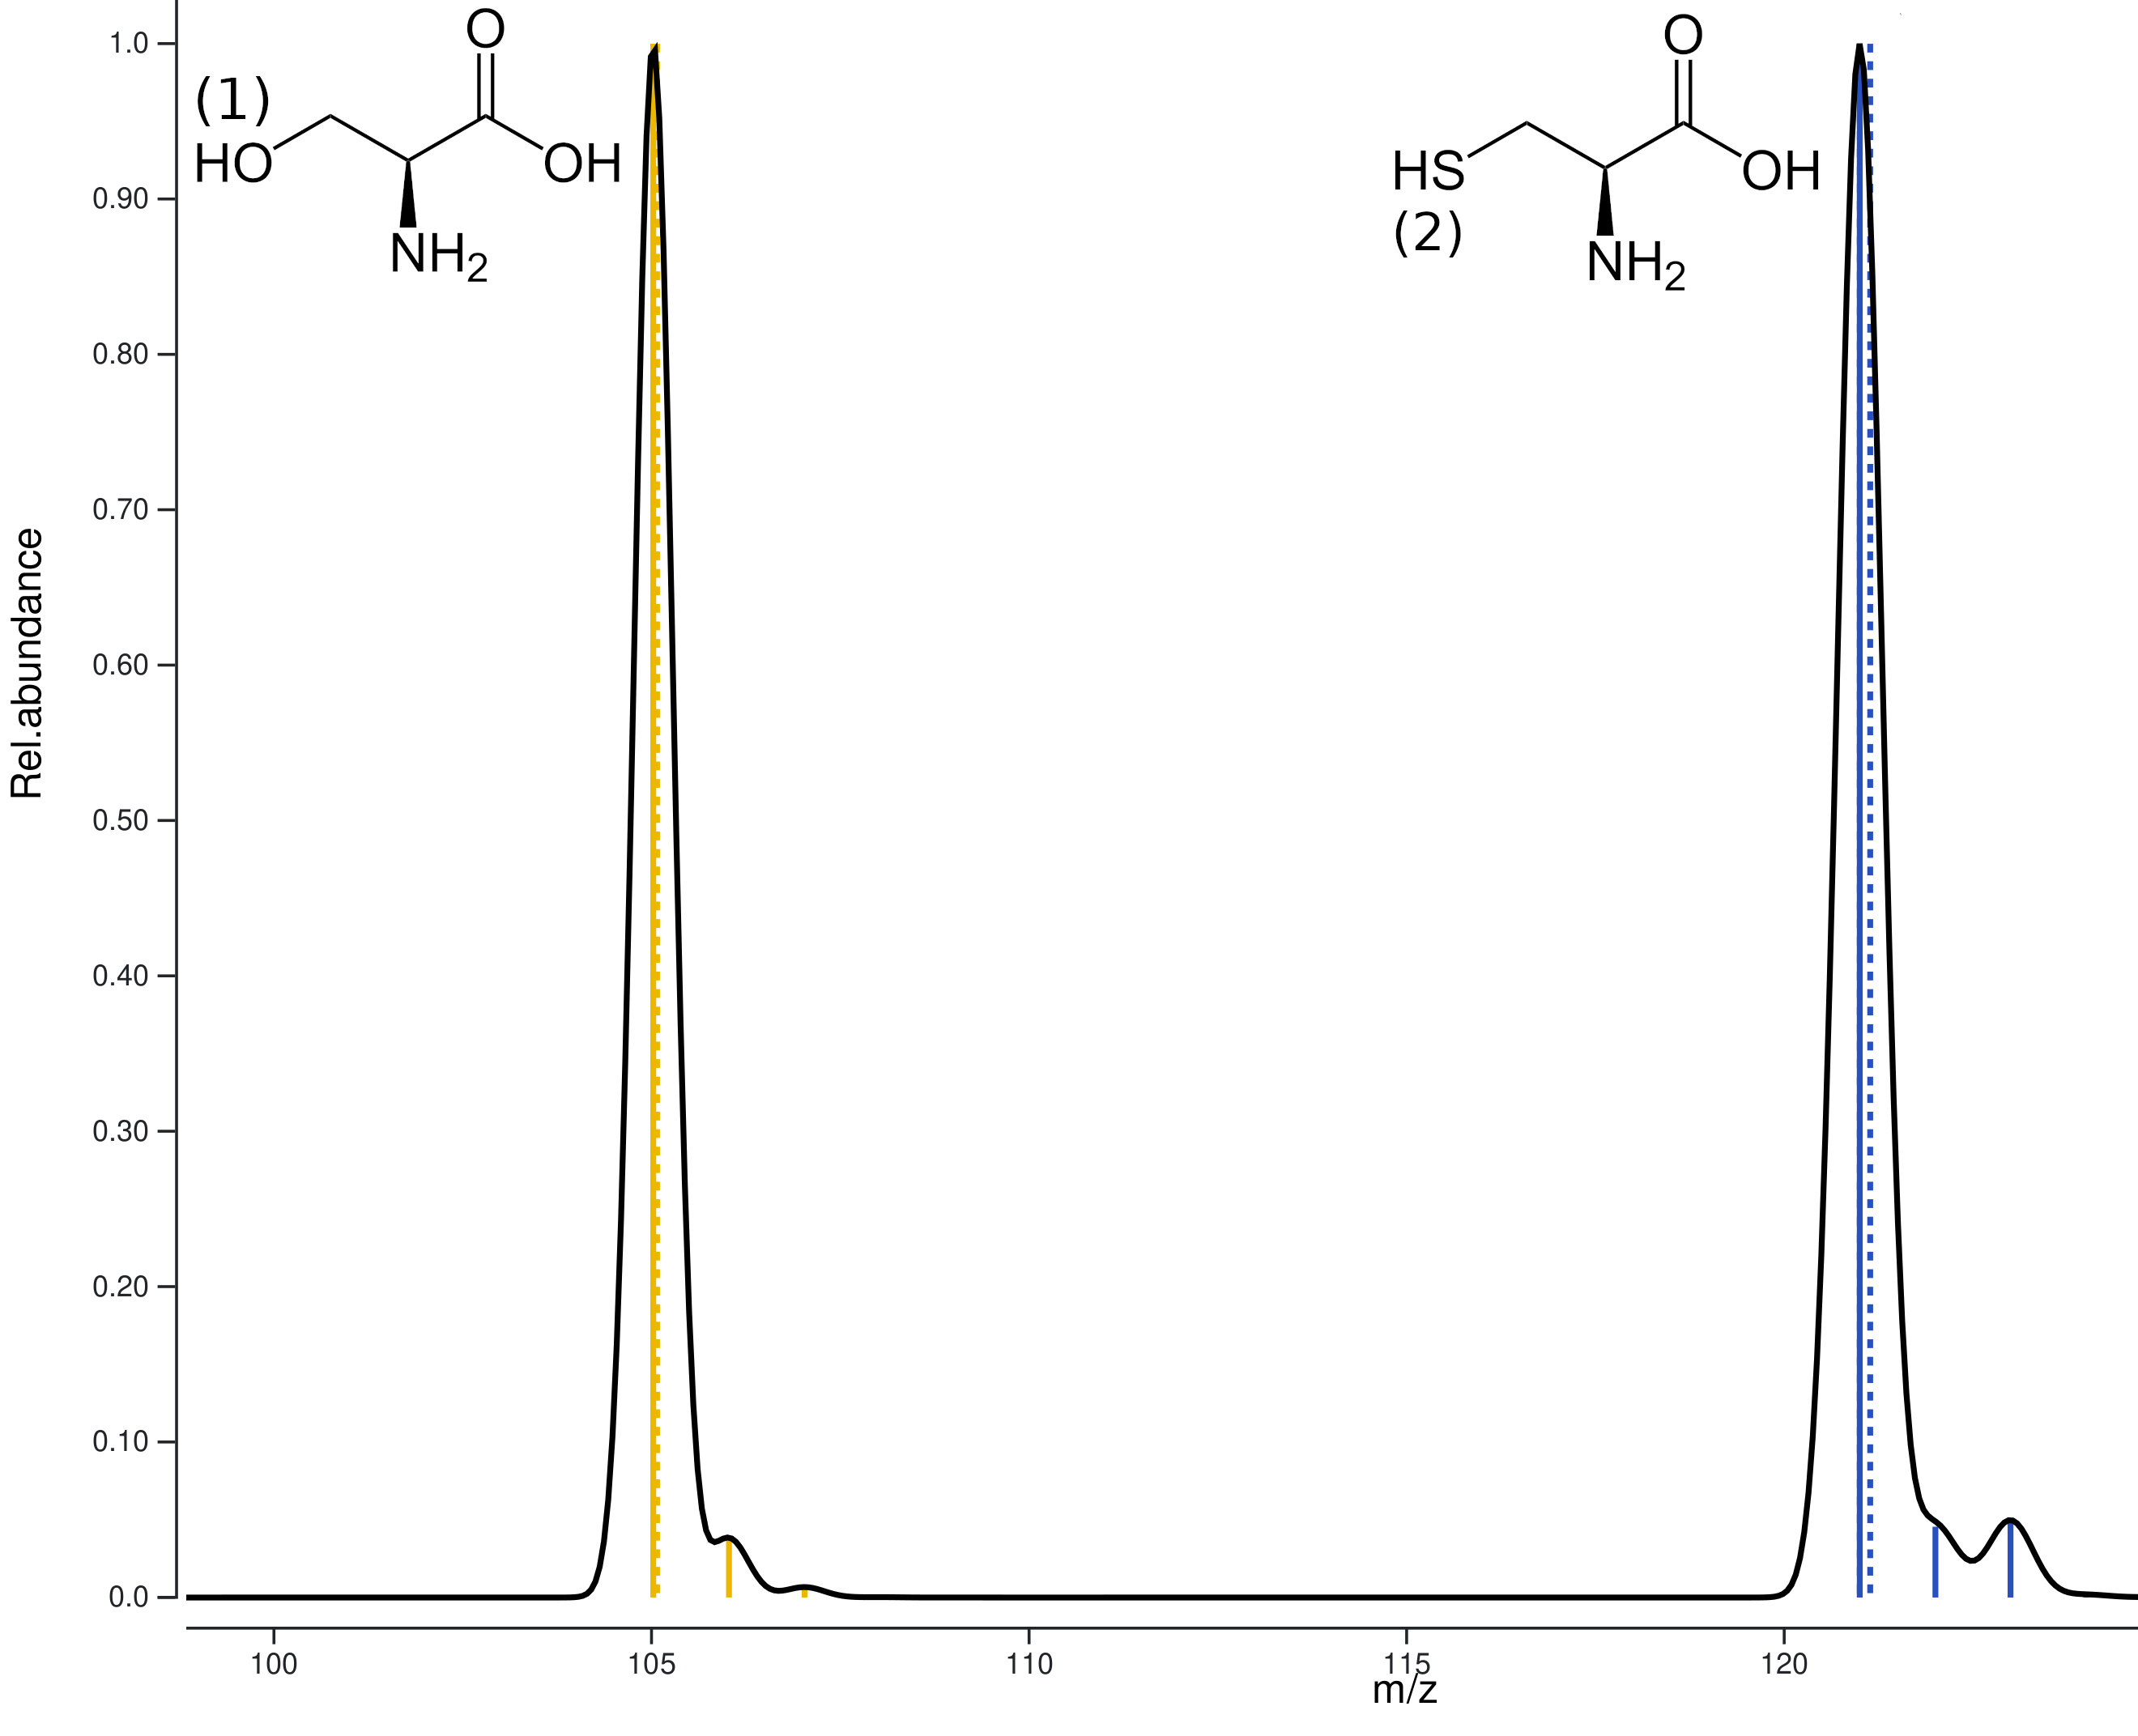
\includegraphics[width=0.75\textwidth]{./Resources/Simulated_Mass_Spectrum.png}
   \centering
   \caption{Computergeneriertes Massenspektrum von der Aminosäure \emph{Serin} (1) und \emph{Cystesin} (2). Peak von \emph{Serin} liegt bei 105; bei \emph{Systesin} um 121. y: relative Häufigkeit}
\end{figure}

Die Maxima werden \gerquot{Peaks} genannt und sind für eine Aminosäure an charakteristischer Position auf der $ x $-Achse. Obwohl sich die beiden Aminosäuren in der Abbildung \ref{fig:Sim_Mass_Spec} nur durch ein Atom unterscheiden (das linke Sauerstoffatom wurde durch ein Schwefelatom ersetzt) sind deren Massenspektren auf der $ x $-Achse weit voneinander entfernt und machen die beiden Aminosäuren dadurch sicher unterscheidbar.\\

Bei einzelnen Aminosäuren funktioniert die MS zuverlässig; bei Peptiden allerdings steht man vor dem Problem, dass das Massenspektrum unübersichtlicher wird und auch Peaks, die von Hintergrundrauschen stammen, schwerer herausgefiltert werden können. Abhilfe schafft hier die Tandem-Massenspektrometrie.

\subsection{Tandem-Massenspektrometrie (MS/MS)}\label{ss:Tandem_MS}
Bei der Tandem-Massenspektrometrie (MS/MS oder MS2) werden zwei MS Vorgänge hintereinander mit einer Probe durchgeführt. Die erste MS dient dazu Ionen aus einem bestimmten \massCharge Bereich auswählbar zu machen. Es entspricht also quasi einer Form der Filterung.

Vor der 2. MS werden die ausgewählten Reste einer Fragmentierung unterzogen. Bei einer Fragmentierung führt man Energie zu mit dem Ziel, dass die Ionen zerfallen und sog. Fragment-Ionen bilden. Diese Fragment-Ionen werden dann auf dem Massenspektrum nach der 2. MS sichtbar gemacht.

Fragment-Ionen sind kleiner als die ursprünglichen Ionen. So kann die 2. MS mit einer höheren Selektivität durchgeführt werden, welches Peaks durch Hintergrundrauschen verringert. Auch lassen sich Ionen besser identifizieren, die ein sehr ähnliches \massCharge-Verhältnis besitzen. Nach der 2. MS liegt eine Fülle an Fragment-Ionen-Peaks vor, aus denen sich die ursprünglichen Strukturinformationen ableiten lassen, da Ionen in spezifische Fragmente zerfallen \cite{Gross2013}. Zusammengefasst kann man sagen, dass das MS/MS Verfahren Ergebnisse höherer Güte erzeugt im Vergleich zur einfachen MS.

\section{De-Novo-Peptidsequenzierung mit \emph{pNovo+}}\label{s:pNovoPlusSeq}
Die \emph{pNovo+} Methode ist eine \gls{gls:DeNovo}, die mit einem \gls{gls:SpecGraph}en für die Auswertung der MS2-Spektren arbeitet und eine Erweiterung des \emph{pNovo} Verfahren darstellt \cite{pNovo}. Der Hauptansatz ist, dass zwei MS/MS Durchläufe mit jeweils verschiedenen Fragmentierungsmethoden\footnote{\emph{pNovo+} verwendet die higher energy
collisional dissociation (HCD) und die electron transfer dissociation (ETD) Fragmentierungsmethoden.} durchgeführt werden. Durch die Wahl einer anderen Fragmentierungsmethode ändert sich auch das MS2-Spektrum. Wenn nun Fragmentierungsmethoden verwendet werden, die möglichst komplementäre Spektren erzeugen, dann lässt sich durch das Zusammenführen der beiden MS2-Spektren die Qualität der Ergebnisse verbessern. Zum Beispiel lassen sich dadurch viele Peaks, die vom Hintergrundrauschen stammen, entfernen.

Für die Ermittlung der Sequenz eines Peptides wird zunächst ein Spektrums-Graph gebildet \dashAndSpace in Form eines DAG (directed acyclic graph). In diesem Graphen wird dann der längste Pfad bei gegebenen Start- und Endknoten berechnet. Die Reihenfolge der Knoten, die im längsten Pfad durchlaufen werden, stellt dann die Peptidsequenz dar.

\subsection{Vorverarbeitung der MS2-Spektren}\label{ss:Vorverarbeitung}
Bevor aus den MS2-Spektren der Spektrums-Graph gebildet werden kann, müssen die Daten vorverarbeitet werden. Für die Auswertung ist es von entscheidener Bedeutung, dass möglichst wenig Peaks verwendet werden, die vom Hintergrundrauschen stammen. Im weiteren Verlauf werden an einem exemplarischen MS2-Spektrum die Verarbeitungsschritte dargestellt.\\

Der erste Schritt ist das Verwenden des natürlichen Logarithmus der Intensitäten. Die Idee dabei ist, dass Hintergrundrauschen nicht überpriorisiert wird.

\begin{figure}[H]
   \centering
   \begin{minipage}[t]{.45\linewidth}
      \centering
      \begin{tikzpicture}[scale=\tikzScale, baseline=(current bounding box.center)]
         \draw [<->,thick] (0,\yAxisHeight) node (yaxis) [above] {\yAxisUnit}
         |- (\xAxisLength,0) node (xaxis) [right] {\xAxisUnit};
\draw[thick] (0.2, 0.0) -- (0.2, 2.3);
\draw[thick] (0.382, 0.0) -- (0.382, 1.7);
\draw[thick] (0.476, 0.0) -- (0.476, 2.7);
\draw[thick] (0.456, 0.0) -- (0.456, 1.8);
\draw[thick] (0.6859999999999999, 0.0) -- (0.6859999999999999, 2.7);
\draw[thick] (0.6839999999999999, 0.0) -- (0.6839999999999999, 1.8);
\draw[thick] (0.752, 0.0) -- (0.752, 1.1);
\draw[thick] (0.8200000000000001, 0.0) -- (0.8200000000000001, 2.2);
\draw[thick] (1.076, 0.0) -- (1.076, 1.5);
\draw[thick] (1.16, 0.0) -- (1.16, 1.9);
\draw[thick] (1.2120000000000002, 0.0) -- (1.2120000000000002, 2.0);
\draw[thick] (1.28, 0.0) -- (1.28, 1.9);
\draw[thick] (1.452, 0.0) -- (1.452, 1.3);
\draw[thick] (1.426, 0.0) -- (1.426, 1.9);
\draw[thick] (1.548, 0.0) -- (1.548, 1.9);
\draw[thick] (1.6740000000000002, 0.0) -- (1.6740000000000002, 1.5);
\draw[thick] (1.788, 0.0) -- (1.788, 2.5);
\draw[thick] (1.856, 0.0) -- (1.856, 2.3);
\draw[thick] (2.036, 0.0) -- (2.036, 1.7);
\draw[thick] (2.142, 0.0) -- (2.142, 1.6);
\draw[thick] (2.2520000000000002, 0.0) -- (2.2520000000000002, 2.0);
\draw[thick] (2.386, 0.0) -- (2.386, 1.6);
\draw[thick] (2.488, 0.0) -- (2.488, 2.9);
\draw[thick] (2.4739999999999998, 0.0) -- (2.4739999999999998, 2.7);
\draw[thick] (2.504, 0.0) -- (2.504, 2.0);
\draw[thick] (2.682, 0.0) -- (2.682, 2.0);
\draw[thick] (2.702, 0.0) -- (2.702, 2.5);
\draw[thick] (2.9259999999999997, 0.0) -- (2.9259999999999997, 2.8);
\draw[thick] (3.024, 0.0) -- (3.024, 2.4);
\draw[thick] (3.096, 0.0) -- (3.096, 1.8);
\draw[thick] (3.244, 0.0) -- (3.244, 2.6);
\draw[thick] (3.362, 0.0) -- (3.362, 1.9);
\draw[thick] (3.46, 0.0) -- (3.46, 2.3);
\draw[thick] (3.516, 0.0) -- (3.516, 1.1);
\draw[thick] (3.584, 0.0) -- (3.584, 1.8);
\draw[thick] (3.652, 0.0) -- (3.652, 2.0);
\draw[thick] (3.838, 0.0) -- (3.838, 1.5);
\draw[thick] (3.8819999999999997, 0.0) -- (3.8819999999999997, 2.6);
\draw[thick] (4.088, 0.0) -- (4.088, 2.6);
\draw[thick] (4.046, 0.0) -- (4.046, 1.1);
\draw[thick] (4.167999999999999, 0.0) -- (4.167999999999999, 2.0);
\draw[thick] (4.266, 0.0) -- (4.266, 2.4);
\draw[thick] (4.38, 0.0) -- (4.38, 1.1);
\draw[thick] (4.456, 0.0) -- (4.456, 2.2);
\draw[thick] (4.644, 0.0) -- (4.644, 2.6);
\draw[thick] (4.675999999999999, 0.0) -- (4.675999999999999, 2.5);
\draw[thick] (4.898000000000001, 0.0) -- (4.898000000000001, 1.2);
   \end{tikzpicture}%
   \end{minipage}%
   \textbf{$\rightarrow$} 
   \begin{minipage}[t]{.45\linewidth}
      \centering
      \begin{tikzpicture}[scale=\tikzScale, baseline=(current bounding box.center)]
      \draw [<->,thick] (0,\yAxisHeight) node (yaxis) [above] {\yAxisUnit}
      |- (\xAxisLength,0) node (xaxis) [right] {\xAxisUnit};
\draw[thick] (0.2, 0.0) -- (0.2, {ln(2.3)});
\draw[thick] (0.382, 0.0) -- (0.382, {ln(1.7)});
\draw[thick] (0.476, 0.0) -- (0.476, {ln(2.7)});
\draw[thick] (0.456, 0.0) -- (0.456, {ln(1.8)});
\draw[thick] (0.6859999999999999, 0.0) -- (0.6859999999999999, {ln(2.7)});
\draw[thick] (0.6839999999999999, 0.0) -- (0.6839999999999999, {ln(1.8)});
\draw[thick] (0.752, 0.0) -- (0.752, {ln(1.1)});
\draw[thick] (0.8200000000000001, 0.0) -- (0.8200000000000001, {ln(2.2)});
\draw[thick] (1.076, 0.0) -- (1.076, {ln(1.5)});
\draw[thick] (1.16, 0.0) -- (1.16, {ln(1.9)});
\draw[thick] (1.2120000000000002, 0.0) -- (1.2120000000000002, {ln(2.0)});
\draw[thick] (1.28, 0.0) -- (1.28, {ln(1.9)});
\draw[thick] (1.452, 0.0) -- (1.452, {ln(1.3)});
\draw[thick] (1.426, 0.0) -- (1.426, {ln(1.9)});
\draw[thick] (1.548, 0.0) -- (1.548, {ln(1.9)});
\draw[thick] (1.6740000000000002, 0.0) -- (1.6740000000000002, {ln(1.5)});
\draw[thick] (1.788, 0.0) -- (1.788, {ln(2.5)});
\draw[thick] (1.856, 0.0) -- (1.856, {ln(2.3)});
\draw[thick] (2.036, 0.0) -- (2.036, {ln(1.7)});
\draw[thick] (2.142, 0.0) -- (2.142, {ln(1.6)});
\draw[thick] (2.2520000000000002, 0.0) -- (2.2520000000000002, {ln(2.0)});
\draw[thick] (2.386, 0.0) -- (2.386, {ln(1.6)});
\draw[thick] (2.488, 0.0) -- (2.488, {ln(2.9)});
\draw[thick] (2.4739999999999998, 0.0) -- (2.4739999999999998, {ln(2.7)});
\draw[thick] (2.504, 0.0) -- (2.504, {ln(2.0)});
\draw[thick] (2.682, 0.0) -- (2.682, {ln(2.0)});
\draw[thick] (2.702, 0.0) -- (2.702, {ln(2.5)});
\draw[thick] (2.9259999999999997, 0.0) -- (2.9259999999999997, {ln(2.8)});
\draw[thick] (3.024, 0.0) -- (3.024, {ln(2.4)});
\draw[thick] (3.096, 0.0) -- (3.096, {ln(1.8)});
\draw[thick] (3.244, 0.0) -- (3.244, {ln(2.6)});
\draw[thick] (3.362, 0.0) -- (3.362, {ln(1.9)});
\draw[thick] (3.46, 0.0) -- (3.46, {ln(2.3)});
\draw[thick] (3.516, 0.0) -- (3.516, {ln(1.1)});
\draw[thick] (3.584, 0.0) -- (3.584, {ln(1.8)});
\draw[thick] (3.652, 0.0) -- (3.652, {ln(2.0)});
\draw[thick] (3.838, 0.0) -- (3.838, {ln(1.5)});
\draw[thick] (3.8819999999999997, 0.0) -- (3.8819999999999997, {ln(2.6)});
\draw[thick] (4.088, 0.0) -- (4.088, {ln(2.6)});
\draw[thick] (4.046, 0.0) -- (4.046, {ln(1.1)});
\draw[thick] (4.167999999999999, 0.0) -- (4.167999999999999, {ln(2.0)});
\draw[thick] (4.266, 0.0) -- (4.266, {ln(2.4)});
\draw[thick] (4.38, 0.0) -- (4.38, {ln(1.1)});
\draw[thick] (4.456, 0.0) -- (4.456, {ln(2.2)});
\draw[thick] (4.644, 0.0) -- (4.644, {ln(2.6)});
\draw[thick] (4.675999999999999, 0.0) -- (4.675999999999999, {ln(2.5)});
\draw[thick] (4.898000000000001, 0.0) -- (4.898000000000001, {ln(1.2)});
      \end{tikzpicture}
      \end{minipage}
      \caption{Anwendung des $ ln $ auf einem exemplarischen MS2-Spektrum.}
\end{figure}

Für das Verständnis des nächsten Schrittes muss man sich in Erinnerung rufen, dass eine gleiche Aminosäure keineswegs immer die gleiche Masse hat. Durch Isotope existiert eine gewisse \gerquot{Massenbandbreite} für ein und dieselbe Aminosäure. MS Systeme sind heute so genau, dass sie diese Differenzen erkennen. Dies hat den ungewollten Effekt, dass mehrere Peaks zu einer Aminosäure gehören können \cite{IsotopicDistributionMS}. Gleichzeitig können die \gerquot{Massenbandbreiten} zweier Aminosäuren sich überschneiden, sodass im ungünstigen Fall zwei Peaks kaum unterscheidbar nebeneinander liegen.\\

Eine Möglichkeit mit dieser Problematik umzugehen ist die Verwendung der monoisotopischen Masse. Die monoisotopische Masse ist die \gerquot{[...] exact mass of the most abundant naturally occurring stable isotope determined relative to the mass of 12 C, which is assigned the exact value of 12.0000.} \cite{MonoisotopicMass}. Ohne dabei jetzt tiefer ins Detail zu gehen kann man sagen, dass alle Peaks, deren Intensität mit einer möglichen monoisotopischen Masse übereinstimmen, auf jeden Fall einer Aminosäure entsprechen und (höchstwahrscheinlich)\footnote{Natürlich ist es möglich, dass das Rauschen zufällig einer monoisotopischen Masse entspricht. Die Wahrscheinlichkeit dafür ist allerdings sehr gering.} kein Hintergrundrauschen sind \cite{MassDefectMS}. Diese Peaks bekommen eine sogennante \emph{charge state}.\\

Der Algorithmus verwendet die \emph{charge state} Peaks als Ausganspunkte für weitere Berechnungen. Wenn die \massCharge Differenz zu einem anderen Peak einem Peptidfragment entspricht, dann stammt dieser Peak höchstwahrscheinlich von einem Fragment. Insgesamt werden damit die relevanten Peptidfragmente herausgeholt. Abbildung \ref{MonoisotopicMassFiltering} zeigt das Ergebnis nach den beiden zuvor genannten Schritten.

\begin{figure}[H]\label{MonoisotopicMassFiltering}
   \centering
   \begin{minipage}[t]{.45\linewidth}
      \centering
      \begin{tikzpicture}[scale=\tikzScale, baseline=(current bounding box.center)]
         \draw [<->,thick] (0,\yAxisHeight) node (yaxis) [above] {\yAxisUnit}
         |- (\xAxisLength,0) node (xaxis) [right] {\xAxisUnit};
\draw[thick] (0.2, 0.0) -- (0.2, {ln(2.3)});
\draw[color=blue!85!,opacity=.55,thick] (0.382, 0.0) -- (0.382, {ln(1.7)});
\draw[color=blue!85!,opacity=.55,thick] (0.476, 0.0) -- (0.476, {ln(2.7)});
\draw[color=magenta,thick] (0.456, 0.0) -- (0.456, {ln(1.8)});
\draw[color=blue!85!,opacity=.55,thick] (0.6859999999999999, 0.0) -- (0.6859999999999999, {ln(2.7)});
\draw[color=blue!85!,opacity=.55,thick] (0.6839999999999999, 0.0) -- (0.6839999999999999, {ln(1.8)});
\draw[thick] (0.752, 0.0) -- (0.752, {ln(1.1)});
\draw[thick] (0.8200000000000001, 0.0) -- (0.8200000000000001, {ln(2.2)});
\draw[thick] (1.076, 0.0) -- (1.076, {ln(1.5)});
\draw[thick] (1.16, 0.0) -- (1.16, {ln(1.9)});
\draw[thick] (1.2120000000000002, 0.0) -- (1.2120000000000002, {ln(2.0)});
\draw[thick] (1.28, 0.0) -- (1.28, {ln(1.9)});
\draw[color=blue!85!,opacity=.55,thick] (1.452, 0.0) -- (1.452, {ln(1.3)});
\draw[color=blue!85!,opacity=.55,thick] (1.426, 0.0) -- (1.426, {ln(1.9)});
\draw[color=magenta,thick] (1.548, 0.0) -- (1.548, {ln(1.9)});
\draw[color=blue!85!,opacity=.55,thick] (1.6740000000000002, 0.0) -- (1.6740000000000002, {ln(1.5)});
\draw[color=blue!85!,opacity=.55,thick] (1.788, 0.0) -- (1.788, {ln(2.5)});
\draw[thick] (1.856, 0.0) -- (1.856, {ln(2.3)});
\draw[thick] (2.036, 0.0) -- (2.036, {ln(1.7)});
\draw[thick] (2.142, 0.0) -- (2.142, {ln(1.6)});
\draw[thick] (2.2520000000000002, 0.0) -- (2.2520000000000002, {ln(2.0)});
\draw[thick] (2.386, 0.0) -- (2.386, {ln(1.6)});
\draw[color=blue!85!,opacity=.55,thick] (2.488, 0.0) -- (2.488, {ln(2.9)});
\draw[thick] (2.4739999999999998, 0.0) -- (2.4739999999999998, {ln(2.7)});
\draw[color=blue!85!,opacity=.55,thick] (2.504, 0.0) -- (2.504, {ln(2.0)});
\draw[color=magenta,thick] (2.682, 0.0) -- (2.682, {ln(2.0)});
\draw[color=blue!85!,opacity=.55,thick] (2.702, 0.0) -- (2.702, {ln(2.5)});
\draw[thick] (2.9259999999999997, 0.0) -- (2.9259999999999997, {ln(2.8)});
\draw[thick] (3.024, 0.0) -- (3.024, {ln(2.4)});
\draw[thick] (3.096, 0.0) -- (3.096, {ln(1.8)});
\draw[thick] (3.244, 0.0) -- (3.244, {ln(2.6)});
\draw[thick] (3.362, 0.0) -- (3.362, {ln(1.9)});
\draw[color=blue!85!,opacity=.55,thick] (3.46, 0.0) -- (3.46, {ln(2.3)});
\draw[color=blue!85!,opacity=.55,thick] (3.516, 0.0) -- (3.516, {ln(1.1)});
\draw[color=blue!85!,opacity=.55,thick] (3.584, 0.0) -- (3.584, {ln(1.8)});
\draw[color=magenta,thick] (3.652, 0.0) -- (3.652, {ln(2.0)});
\draw[color=blue!85!,opacity=.55,thick] (3.838, 0.0) -- (3.838, {ln(1.5)});
\draw[color=blue!85!,opacity=.55,thick] (3.8819999999999997, 0.0) -- (3.8819999999999997, {ln(2.6)});
\draw[thick] (4.088, 0.0) -- (4.088, {ln(2.6)});
\draw[thick] (4.046, 0.0) -- (4.046, {ln(1.1)});
\draw[thick] (4.167999999999999, 0.0) -- (4.167999999999999, {ln(2.0)});
\draw[thick] (4.266, 0.0) -- (4.266, {ln(2.4)});
\draw[color=blue!85!,opacity=.55,thick] (4.38, 0.0) -- (4.38, {ln(1.1)});
\draw[color=blue!85!,opacity=.55,thick] (4.456, 0.0) -- (4.456, {ln(2.2)});
\draw[color=magenta,thick] (4.644, 0.0) -- (4.644, {ln(2.6)});
\draw[color=blue!85!,opacity=.55,thick] (4.675999999999999, 0.0) -- (4.675999999999999, {ln(2.5)});
\draw[color=blue!85!,opacity=.55,thick] (4.898000000000001, 0.0) -- (4.898000000000001, {ln(1.2)});
   \end{tikzpicture}%
   \end{minipage}%
   \textbf{$\rightarrow$} 
   \begin{minipage}[t]{.45\linewidth}
      \centering
      \begin{tikzpicture}[scale=\tikzScale, baseline=(current bounding box.center)]
      \draw [<->,thick] (0,\yAxisHeight) node (yaxis) [above] {\yAxisUnit}
      |- (\xAxisLength,0) node (xaxis) [right] {\xAxisUnit};
\draw[color=blue!85!,opacity=.55,thick] (0.382, 0.0) -- (0.382, {ln(1.7)});
\draw[color=blue!85!,opacity=.55,thick] (0.476, 0.0) -- (0.476, {ln(2.7)});
\draw[color=magenta,thick] (0.456, 0.0) -- (0.456, {ln(1.8)});
\draw[color=blue!85!,opacity=.55,thick] (0.6859999999999999, 0.0) -- (0.6859999999999999, {ln(2.7)});
\draw[color=blue!85!,opacity=.55,thick] (0.6839999999999999, 0.0) -- (0.6839999999999999, {ln(1.8)});
\draw[color=blue!85!,opacity=.55,thick] (1.452, 0.0) -- (1.452, {ln(1.3)});
\draw[color=blue!85!,opacity=.55,thick] (1.426, 0.0) -- (1.426, {ln(1.9)});
\draw[color=magenta,thick] (1.548, 0.0) -- (1.548, {ln(1.9)});
\draw[color=blue!85!,opacity=.55,thick] (1.6740000000000002, 0.0) -- (1.6740000000000002, {ln(1.5)});
\draw[color=blue!85!,opacity=.55,thick] (1.788, 0.0) -- (1.788, {ln(2.5)});
\draw[color=blue!85!,opacity=.55,thick] (2.488, 0.0) -- (2.488, {ln(2.9)});
\draw[color=blue!85!,opacity=.55,thick] (2.504, 0.0) -- (2.504, {ln(2.0)});
\draw[color=magenta,thick] (2.682, 0.0) -- (2.682, {ln(2.0)});
\draw[color=blue!85!,opacity=.55,thick] (2.702, 0.0) -- (2.702, {ln(2.5)});
\draw[color=blue!85!,opacity=.55,thick] (3.46, 0.0) -- (3.46, {ln(2.3)});
\draw[color=blue!85!,opacity=.55,thick] (3.516, 0.0) -- (3.516, {ln(1.1)});
\draw[color=blue!85!,opacity=.55,thick] (3.584, 0.0) -- (3.584, {ln(1.8)});
\draw[color=magenta,thick] (3.652, 0.0) -- (3.652, {ln(2.0)});
\draw[color=blue!85!,opacity=.55,thick] (3.838, 0.0) -- (3.838, {ln(1.5)});
\draw[color=blue!85!,opacity=.55,thick] (3.8819999999999997, 0.0) -- (3.8819999999999997, {ln(2.6)});
\draw[color=blue!85!,opacity=.55,thick] (4.38, 0.0) -- (4.38, {ln(1.1)});
\draw[color=blue!85!,opacity=.55,thick] (4.456, 0.0) -- (4.456, {ln(2.2)});
\draw[color=magenta,thick] (4.644, 0.0) -- (4.644, {ln(2.6)});
\draw[color=blue!85!,opacity=.55,thick] (4.675999999999999, 0.0) -- (4.675999999999999, {ln(2.5)});
\draw[color=blue!85!,opacity=.55,thick] (4.898000000000001, 0.0) -- (4.898000000000001, {ln(1.2)});
      \end{tikzpicture}
      \end{minipage}
      \caption{Entfernen von Peaks, die keiner monoisotopischen Masse entsprechen oder benachbart mit einer Differenz von einem Fragment-Ion sind.}
\end{figure}

Tatsächlich ist die Verarbeitung an dieser Stelle noch etwas komplexer. So existieren auch noch sogenannte \emph{isotopic cluster}\footnote{Definition eines \emph{isotopic cluster} nach IUPAC: \gerquot{Group of peaks representing ions of the same elemental composition, but different isotopic compositions.} \cite[1556]{IUPACDefinitions}}, die gesondert verarbeitet werden. Für das grundsätzliche Prinzip ist dieses Detail allerdings weniger relevant.\\

Im letzten Vorberarbeitungsschritt werden Peaks aus einem irrelevanten \massCharge Bereich entfernt und naheliegende Peaks werden zusammengefasst, indem der Mittelwert sowol des \massCharge Wertes als auch der der Intensität besimmt wird. Üblicherweise liegt der Bereich für das Zusammenfassen bei $ +- 20 ppm $.

\begin{figure}[H]
   \centering
   \begin{minipage}[t]{.45\linewidth}
      \centering
      \begin{tikzpicture}[scale=\tikzScale, baseline=(current bounding box.center)]
         \draw [<->,thick] (0,\yAxisHeight) node (yaxis) [above] {\yAxisUnit}
         |- (\xAxisLength,0) node (xaxis) [right] {\xAxisUnit};
\draw[thick] (0.382, 0.0) -- (0.382, {ln(1.7)});
\draw[thick] (0.476, 0.0) -- (0.476, {ln(2.7)});
\draw[thick] (0.456, 0.0) -- (0.456, {ln(1.8)});
\draw[thick] (0.6859999999999999, 0.0) -- (0.6859999999999999, {ln(2.7)});
\draw[thick] (0.6839999999999999, 0.0) -- (0.6839999999999999, {ln(1.8)});
\draw[color=red,thick] (1.452, 0.0) -- (1.452, {ln(1.3)});
\draw[color=red,thick] (1.426, 0.0) -- (1.426, {ln(1.9)});
\draw[thick] (1.548, 0.0) -- (1.548, {ln(1.9)});
\draw[thick] (1.6740000000000002, 0.0) -- (1.6740000000000002, {ln(1.5)});
\draw[thick] (1.788, 0.0) -- (1.788, {ln(2.5)});
\draw[color=red,thick] (2.488, 0.0) -- (2.488, {ln(2.9)});
\draw[color=red,thick] (2.504, 0.0) -- (2.504, {ln(2.0)});
\draw[color=red,thick] (2.682, 0.0) -- (2.682, {ln(2.0)});
\draw[color=red,thick] (2.702, 0.0) -- (2.702, {ln(2.5)});
\draw[thick] (3.46, 0.0) -- (3.46, {ln(2.3)});
\draw[thick] (3.516, 0.0) -- (3.516, {ln(1.1)});
\draw[thick] (3.584, 0.0) -- (3.584, {ln(1.8)});
\draw[thick] (3.652, 0.0) -- (3.652, {ln(2.0)});
\draw[color=red,thick] (3.838, 0.0) -- (3.838, {ln(1.5)});
\draw[color=red,thick] (3.8819999999999997, 0.0) -- (3.8819999999999997, {ln(2.6)});
\draw[thick] (4.38, 0.0) -- (4.38, {ln(1.1)});
\draw[thick] (4.456, 0.0) -- (4.456, {ln(2.2)});
\draw[thick] (4.644, 0.0) -- (4.644, {ln(2.6)});
\draw[thick] (4.675999999999999, 0.0) -- (4.675999999999999, {ln(2.5)});
\draw[thick] (4.898000000000001, 0.0) -- (4.898000000000001, {ln(1.2)});

\fill[red!25!,opacity=.25] (0,0) rectangle (1,\yAxisHeight-\axisColorOffset);
         \fill[red!25!,opacity=.25] (\xAxisLength-1,0) rectangle (\xAxisLength-\axisColorOffset,\yAxisHeight-\axisColorOffset);
         \fill[green!25!,opacity=.25] (1,0) rectangle (\xAxisLength-1,\yAxisHeight-\axisColorOffset);
   \end{tikzpicture}%
   \end{minipage}%
   \textbf{$\rightarrow$} 
   \begin{minipage}[t]{.45\linewidth}
      \centering
      \begin{tikzpicture}[scale=\tikzScale, baseline=(current bounding box.center)]
      \draw [<->,thick] (0,\yAxisHeight) node (yaxis) [above] {\yAxisUnit}
      |- (\xAxisLength,0) node (xaxis) [right] {\xAxisUnit};
%\draw[color=red,thick] (1.452, 0.0) -- (1.452, {ln(1.3)});
%\draw[color=red,thick] (1.426, 0.0) -- (1.426, {ln(1.9)});
\draw[color=red,ultra thick] ({(1.452+1.426)/2}, 0.0) -- ({(1.452+1.426)/2}, {(ln(1.3)+ln(1.9))/2});

\draw[thick] (1.548, 0.0) -- (1.548, {ln(1.9)});
\draw[thick] (1.6740000000000002, 0.0) -- (1.6740000000000002, {ln(1.5)});
\draw[thick] (1.788, 0.0) -- (1.788, {ln(2.5)});

%\draw[color=red,thick] (2.488, 0.0) -- (2.488, {ln(2.9)});
%\draw[color=red,thick] (2.504, 0.0) -- (2.504, {ln(2.0)});
\draw[color=red,ultra thick] ({(2.488+2.504)/2}, 0.0) -- ({(2.488+2.504)/2}, {(ln(2.9)+ln(2.0))/2});

%\draw[color=red,thick] (2.682, 0.0) -- (2.682, {ln(2.0)});
%\draw[color=red,thick] (2.702, 0.0) -- (2.702, {ln(2.5)});
\draw[color=red,ultra thick] ({(2.682+2.702)/2}, 0.0) -- ({(2.682+2.702)/2}, {(ln(2.0+ln(2.5))/2});

\draw[thick] (3.46, 0.0) -- (3.46, {ln(2.3)});
\draw[thick] (3.516, 0.0) -- (3.516, {ln(1.1)});
\draw[thick] (3.584, 0.0) -- (3.584, {ln(1.8)});
\draw[thick] (3.652, 0.0) -- (3.652, {ln(2.0)});

%\draw[color=red,thick] (3.838, 0.0) -- (3.838, {ln(1.5)});
%\draw[color=red,thick] (3.8819999999999997, 0.0) -- (3.8819999999999997,{ln(2.6)});
\draw[color=red,ultra thick] ({(3.838+3.8819999999999997)/2}, 0.0) -- ({(3.838+3.8819999999999997)/2}, {(ln(1.5)+ln(2.6))/2});

\fill[red!25!,opacity=.25] (0,0) rectangle (1,\yAxisHeight-\axisColorOffset);
         \fill[red!25!,opacity=.25] (\xAxisLength-1,0) rectangle (\xAxisLength-\axisColorOffset,\yAxisHeight-\axisColorOffset);
         \fill[green!25!,opacity=.25] (1,0) rectangle (\xAxisLength-1,\yAxisHeight-\axisColorOffset);
      \end{tikzpicture}
      \end{minipage}
      \caption{Entfernen von Peaks aus einem irrelevanten \massCharge Bereich und zusammenfassen naheliegender Peaks. Rot markierte Peaks sind jene, die zusammengefasst werden.}
\end{figure}

\subsection{Bildung eines Spektrums-Graphen}\label{ss:BildungSpekGraph}
Der Spektrums-Graph wird aus einem vorverarbeiteten MS2-Spektrum (siehe Kapitel: \ref{ss:Vorverarbeitung}) gebildet. Im initialen Zustand werden die Peaks als Knoten interpretiert. Dazu kommt ein Start- und Endknoten. Jedem Knoten wird eine Masse zugeordet; im initialen Zustand bekommt der Startknoten die Masse 0 und der Endknoten die Masse des vorherigen Knotens minus der Masse des Wassers ($ 18,02 $). Die Masse der übrigen Knoten entsprechen ihren jeweils korrespondierenden \massCharge Wert. Die gerichteten Kanten werden zwischen einem Knotenpaar hinzugefügt, wenn die Differenz deren Masse gleich ist mit der Masse von ein oder zwei Aminosäuren.

\subsection{Identifikation der Aminosäuresequenz}
Der gebildete DAG kann mit klassischen Algorithmen, die den längsten Pfad suchen, durchlaufen werden. Bezogen auf die Graphentheorie entspricht die Ermittlung der Aminosäurensequenz dem Suchen eines bestimmten Pfades \dashAndSpace und nicht nach irgendeinem Pfad. Daher muss der Algorithmus mittels einer Breitensuche arbeiten, um alle möglichen Pfade zu bestimmen.

In aller Regel wird es mehrere Pfade geben. Bestimmte Sequenzen sind wahrscheinlicher als andere. So sind Pfade mit Kanten, die wegen der Massendifferenz von genau einer Aminosäure gebildet wurden, wahrscheinlicher \cite{pNovoPlus}. Alle Pfade bekommen mittels einer Scoring-Funktion einen Wert zugewiesen. Der Pfad mit dem höchsten Scoring-Wert ist wahrscheinlich das richtige Ergebnis. Die Scoring-Funktion berücksichtigt unter anderem wie viele Fragmente, die einer bestimmten Aminosäure zugeordet werden können, im MS2-Spektrum vorhanden sind \cite{pNovo}. Die Sequenz mit dem höchsten Scoring-Wert ist das Endergebnis.

\section{De-Novo-Peptidsequenzierung mit \emph{Open-pNovo}}\label{s:OpenpNovoSeq}
Bei Proteinen können posttranslationale Proteinmodifikationen (PTM) auftreten. PTMs sind Ereignisse, bei denen sich Änderungen im Protein einstellen \cite{Mann2003}; teilweise sind die Änderungen von einer Zelle erwünscht \dashAndSpace teilweise stammen sie aber auch zum Beispiel von unerwünschten Wechselwirkungen nebeneinanderliegenden Aminosäuren. Ein Teil dieser PTMs führen zu einer Änderung der Aminosäuresequenz. Dies ist für die \gls{gls:DeNovo} nicht weiter problematisch, da sowieso ohne eine Datenbank gearbeitet wird, sodass solche PTMs nicht einmal auffallen würden. Andere PTMs hingegen haben die Auswirkung, dass Stoffe gebildet werden, die nicht mehr zu der Gruppe der proteinogenen Aminosäuren gehören. Proteinogene Aminosäuren sind jene Aminosäuren, die für den Bau von Proteinen verwendet werden. Der Effekt ist also, dass Stoffe (oder deren Fragmente) bei einem Massenspektrum angezeigt werden, die kein Teil eines Peptids sein können. Bei der Sequenzierung von Peptidfragmenten muss dies daher berücksichtigt werden.
Wenn im weiteren Verlauf von PTMs gesprochen wird, dann sind solche gemeint, die für die \gls{gls:DeNovo} relevant sind.

Open-pNovo ist ein \gls{gls:DeNovo}sverfahren, welches auf pNovo+ Tool aufbaut und versucht die Problematik mit den PTMs zu lösen.

\subsection{PTMs im konstruierten DAG}
Die Konvertierung eines MS2-Spektrums läuft bis zum DAG analog ab wie in den Kapiteln \ref{ss:Vorverarbeitung} und \ref{ss:BildungSpekGraph} für pNovo+. Der Unterschied ist nun, dass es zwei Arten von Kanten gibt:

\begin{itemize}
   \item \gerquot{Normale} Kanten: Kanten, die gebildet werden, wie es bereits für \emph{pNovo+} gezeigt wurde. 
   \item \gerquot{Modifizierte} Kanten: Kanten, die zum Grahpen hinzugefügt werden, wenn die Massendifferenz zweier Knoten der Masse einer Aminosäure plus der Masse einer möglichen PTM-Änderung entspricht. 
\end{itemize}

Eine Liste aller PTMs in der Datenbank Unimod (sowohl relevante als auch nicht relevante) beinhaltet aktuell 1510 Einträge\footnote{Siehe: \url{https://www.ebi.ac.uk/ols/ontologies/unimod}} (Stand: 18.04.2022). Für die modifizierten Kanten gibt es insgesamt $ 1510 * 20 = 30200 $ mögliche Differenzen, wobei viele davon nicht relevante PTMs sind. Zum Vergleich: bei den normalen Kanten gibt es $ 20^2 = 400 $ mögliche Differenzen.

Die hohe Anzahl an Differenzen für modifizierte Kanten hat die Konsequenz, dass viele Knoten zufällig verbunden werden und dass dadurch die Genauigkeit der Ergebnisse abnimmt. Dieses Problem kann man durch eine geringere Liste an möglichen PTMs abfedern, allerdings mit einem Verlust  der Genauigkeit auf Seiten der PTMs. Es ist hier also eine Abwägung.

\subsection{Evaluierung von Open-pNovo}
Open-pNovo wurde sowohl auf drei realen als auch auf drei generierten Testdaten getestet. Tabelle \ref{tab:OpenPNovoResults} zeigt die Ergebnisse im Vergleich zu pNovo+ und zwei anderen Algorithmen. Die Datensätze enthielten die am häufigsten vorkommenden PTMs.

\begin{table}[H]
    \centering
    \begin{tabular}{l|c|c|c|c}
        \toprule
        \textbf{Testdatensätze} & \textbf{Open-pNovo+} & \textbf{pNovo+} & \textbf{PEAKS} & \textbf{Novor} \\
        \midrule
        Real (20259) & $76,3 \%$ & $68,5 \%$ & $65,8 \%$ & $39,9 \%$ \\
        Generiert (17877) & $77,8 \%$ & $0,6 \%$ & $0,5 \%$ & $0,2 \%$ \\
        \bottomrule
    \end{tabular}
    \newline
    \caption{Vergleich der durchschnittlichen richtigen \gls{gls:DeNovo} Peptidsequenzierungen von Open-pNovo und anderen Algorithmen \cite[650]{OpenPNovo}.}
    \label{tab:OpenPNovoResults}
\end{table}

Die enorm schlechten Ergebnisse der anderen Algorithmen bei den generierten Testdaten ist ein Nebeneffekt des Ziels bei der Testdatengenerierung. Denn diese wurden so ausgelegt, um die Grenzen von Open-pNovo+ zu ermitteln \cite[649]{OpenPNovo}. Eine Aussagekraft haben diese Ergebnisse also nicht. Allerdings auch bei realen Testdaten zeigt sich Open-pNovo als voll konkurrenzfähig gegenüber den anderen Algorithmen.

Noch besser zeigt sich Open-pNovo, wenn der Recall Wert betrachtet wird \dashAndSpace also die Anzahl an verschiedenen PSMs, die erkannt wurden. In diesem Fall ist der Abstand zu den anderen Algorithmen deutlich größer geworden.

\begin{table}[H]
    \centering
    \begin{tabular}{l|c|c|c|c}
        \toprule
        \textbf{Testdatensätze} & \textbf{Open-pNovo+} & \textbf{pNovo+} & \textbf{PEAKS} & \textbf{Novor} \\
        \midrule
        Real (5034) & $61,6 \%$ & $31,3 \%$ & $32,0 \%$ & $13,7 \%$ \\
        \bottomrule
    \end{tabular}
    \newline
    \caption{Vergleich der durchschnittlichen Recall Werte einer \gls{gls:DeNovo} Peptidsequenzierungen von Open-pNovo und anderen Algorithmen \cite[650]{OpenPNovo}.}
    \label{tab:OpenPNovoResultsRecall}
\end{table}

\subsection{Zusammenfassung}


% Die \gls{gls:DeNovo} nutzt die sogenannte \gls{gls:TMassSpek} für die Bestimmung der Peptidsequenz. Dabei wird die physikalische Eigenschaft ausgenutzt, dass jedes Atom bzw. jedes Molekül \dashAndSpace wenn es einer \gls{gls:Ionisation} unterzogen wurde \dashAndSpace ein charakteristisches \gls{gls:MassSpek} besitzt. Das \gls{gls:MassSpek} stellt also eine Art \gerquot{Fingerabdruck} eines Moleküls dar und macht dieses ermittelbar.

% U.U. eine Beispielgrafik eines Massenspektrums hinzufuegen ...

\subsubsection{\glsentrytext{gls:TMassSpek} bei größeren Molekülen}
Bei größeren Molekülen (wie einem Protein) führt die \gls{gls:Ionisation} dazu, dass das Molekül in kleinere spezifische Ionen zerfällt (sog. Fragmentierung). Die Fragmentierungsinformationen einer \gls{gls:DeNovo} sind meist unvollständig, da fehlende Daten bei einem Fragmentierungsschritt die Güte des Endergebnisses negativ beeinflusst. Dies wird insbesondere dann ein Problem, wenn unbekannte Änderungen in einer Peptidsequenz vorhanden sind.

Um dieses Problem zu verringern können unterschiedliche Techniken parallel eingesetzt werden, welche verschiedene Fragmente erzeugen und daher auch verschiedenartige \glspl{gls:MassSpek} zur Folge haben.\footnote{Konkret: Es wird sowohl das \gls{acr:HCD} als auch das \gls{acr:ETD} Verfahren angewendet.}

\subsection{Datenaufbereitung}
Typischerweise betrachtet man die sog. \gerquot{\glspl{gls:Peak}} in den \glspl{gls:MassSpek}. Jeder \gls{gls:Peak} stellt ein unterschiedliches Ion dar. Dazu kommen Messungenauigkeiten sowie Hintergrundrauschen. Durch die hohe Anzahl an möglichen Ionen kann nicht ohne weiteres differenziert werden, welcher der \glspl{gls:Peak} von welchen Ionen erzeugt wurden und welche nicht.

% Frage an Dominik: Ist hier eine einfache Auflistung an Techniken für die Datenaufbereitung besser?
Der Algorithmus für die Datenaufbereitung berechnet den natürlichen Logarithmus von den Intensitäten der \glspl{gls:Peak}, um Hintergrundrauschen und Messungenauigkeiten nicht überzupriorisieren. Zusätzlich dazu werden \glspl{gls:Peak}, die in einem Toleranzbereich nebeneinander liegen, zusammengefasst. Am Ende werden die \glspl{gls:Peak} entfernt, bei denen bekannt ist, dass es sich nicht um relevante Ionen handeln kann. (z.B. \glspl{gls:Peak} von Isotopen)

\begin{figure}[H]
   \centering
   \begin{minipage}[t]{.4\linewidth}
      \centering
      \begin{tikzpicture}[scale=\tikzScale, baseline=(current bounding box.center)]
         \draw [<->,thick] (0,2.75) node (yaxis) [above] {\yAxisUnit}
         |- (3,0) node (xaxis) [right] {\xAxisUnit};

         \draw[thick] (0.2,0) -- (0.2,1.1);
         \draw[thick] (0.3,0) -- (0.3,1.6);
         \draw[thick] (0.6,0) -- (0.6,1.7);
         \draw[thick] (0.8,0) -- (0.8,1.2);
         \draw[thick] (1.0,0) -- (1.0,1.1);

         \draw[color=red,thick] (1.2,0) -- (1.2,2.65);
         \draw[thick] (1.4,0) -- (1.4,1.4);
         \draw[thick] (1.6,0) -- (1.6,1.2);
         \draw[thick] (1.8,0) -- (1.8,1.3);
         \draw[thick] (2.0,0) -- (2.0,1.8);

         \draw[thick] (1.1,0) -- (1.1,2.0);
         \draw[color=red,thick] (0.35,0) -- (0.35,2.25);
         \draw[thick] (1.9,0) -- (1.9,1.4);
         \draw[color=red,thick] (2.2,0) -- (2.2,2.6);
         \draw[thick] (2.5,0) -- (2.5,1.25);

         \draw[thick] (2.7,0) -- (2.7,1.1);
         \foreach \x in {1,...,6}
         {
            \draw[thick] (1.2+\x*0.05,0) -- (1.2+\x*0.05,1.0+\x*0.15);
         }
      \end{tikzpicture}%
      % \subcaption{Exemplarische Rohdaten}
   \end{minipage}%
   \textbf{$\rightarrow$}
   \begin{minipage}[t]{.4\linewidth}
      \centering
      \begin{tikzpicture}[scale=\tikzScale, baseline=(current bounding box.center)]
         \draw [<->,thick] (0,2.75) node (yaxis) [above] {\yAxisUnit}
         |- (3,0) node (xaxis) [right] {\xAxisUnit};

         \draw[thick] (0.2,0) -- (0.2,{ln(1.1)});
         \draw[thick] (0.3,0) -- (0.3,{ln(1.6)});
         \draw[thick] (0.6,0) -- (0.6,{ln(1.7)});
         \draw[thick] (0.8,0) -- (0.8,{ln(1.2)});
         \draw[thick] (1.0,0) -- (1.0,{ln(1.1)});

         \draw[color=red,thick] (1.2,0) -- (1.2,{ln(2.65)});
         \draw[thick] (1.4,0) -- (1.4,{ln(1.4)});
         \draw[thick] (1.6,0) -- (1.6,{ln(1.2)});
         \draw[thick] (1.8,0) -- (1.8,{ln(1.3)});
         \draw[thick] (2.0,0) -- (2.0,{ln(1.8)});

         \draw[thick] (1.1,0) -- (1.1,{ln(2.0)});
         \draw[color=red,thick] (0.35,0) -- (0.35,{ln(2.25)});
         \draw[thick] (1.9,0) -- (1.9,{ln(1.4)});
         \draw[color=red,thick] (2.2,0) -- (2.2,{ln(2.6)});
         \draw[thick] (2.5,0) -- (2.5,{ln(1.25)});

         \draw[thick] (2.7,0) -- (2.7,{ln(1.1)});
         \foreach \x in {1,...,6}
         {%
            \draw[thick] (1.2+\x*0.05,0) -- (1.2+\x*0.05,{ln(1.0+\x*0.15)});
         }
      \end{tikzpicture}
      %\subcaption{Exemplarische Rohdaten}
   \end{minipage}
   \caption{Anwendung des $ln$ auf Rohdaten. Rote \glspl{gls:Peak} stellen hier exemplarisch fehlerhafte Daten dar, die nach dem $ln$ reduziert wurden.}
\end{figure}

\begin{figure}[H]
   \centering
   \begin{minipage}[t]{.4\linewidth}
      \centering
      \begin{tikzpicture}[scale=\tikzScale, baseline=(current bounding box.center)]
         \draw [<->,thick] (0,2.75) node (yaxis) [above] {\yAxisUnit}
         |- (3,0) node (xaxis) [right] {\xAxisUnit};

         \draw[thick] (0.2,0) -- (0.2,{ln(1.1)});
         \draw[thick] (0.3,0) -- (0.3,{ln(1.6)});
         \draw[thick] (0.6,0) -- (0.6,{ln(1.7)});
         \draw[thick] (0.8,0) -- (0.8,{ln(1.2)});
         \draw[thick] (1.0,0) -- (1.0,{ln(1.1)});

         \draw[thick] (1.2,0) -- (1.2,{ln(2.65)});
         \draw[thick] (1.4,0) -- (1.4,{ln(1.4)});
         \draw[thick] (1.6,0) -- (1.6,{ln(1.2)});
         \draw[thick] (1.8,0) -- (1.8,{ln(1.3)});
         \draw[thick] (2.0,0) -- (2.0,{ln(1.8)});

         \draw[thick] (1.1,0) -- (1.1,{ln(2.0)});
         \draw[thick] (0.35,0) -- (0.35,{ln(2.25)});
         \draw[thick] (1.9,0) -- (1.9,{ln(1.4)});
         \draw[thick] (2.2,0) -- (2.2,{ln(2.6)});
         \draw[thick] (2.5,0) -- (2.5,{ln(1.25)});

         \draw[thick] (2.7,0) -- (2.7,{ln(1.1)});
         \foreach \x in {1,...,6}
         {%
            \draw[color=red,thick] (1.2+\x*0.05,0) -- (1.2+\x*0.05,{ln(1.0+\x*0.15)});
         }

         \draw[dotted] (0.4,0) -- (0.4,2.75);
         \draw[dotted] (2.6,0) -- (2.6,2.75);
         \fill[red!25!,opacity=.25] (0,0) rectangle (0.4,2.75);
         \fill[red!25!,opacity=.25] (2.6,0) rectangle (3.0,2.75);
         \fill[green!25!,opacity=.25] (0.4,0) rectangle (2.6,2.75);
      \end{tikzpicture}
      %\subcaption{Exemplarische Rohdaten}
   \end{minipage}
   \textbf{$\rightarrow$}
   \begin{minipage}[t]{.4\linewidth}
      \centering
      \begin{tikzpicture}[scale=\tikzScale, baseline=(current bounding box.center)]
         \draw [<->,thick] (0,2.75) node (yaxis) [above] {\yAxisUnit}
         |- (3,0) node (xaxis) [right] {\xAxisUnit};

         \draw[thick] (0.6,0) -- (0.6,{ln(1.7)});
         \draw[thick] (0.8,0) -- (0.8,{ln(1.2)});
         \draw[thick] (1.0,0) -- (1.0,{ln(1.1)});

         \draw[thick] (1.2,0) -- (1.2,{ln(2.65)});
         %\draw[thick] (1.4,0) -- (1.4,{ln(1.4)});
         \draw[thick] (1.6,0) -- (1.6,{ln(1.2)});
         \draw[thick] (1.8,0) -- (1.8,{ln(1.3)});
         \draw[thick] (2.0,0) -- (2.0,{ln(1.8)});

         \draw[thick] (1.1,0) -- (1.1,{ln(2.0)});
         \draw[thick] (1.9,0) -- (1.9,{ln(1.4)});
         \draw[thick] (2.2,0) -- (2.2,{ln(2.6)});
         \draw[thick] (2.5,0) -- (2.5,{ln(1.25)});

         \draw[color=red,ultra thick] (1.2+1*0.05,0) -- (1.2+1*0.05,{ln(1.0+1*0.15)});
         \draw[color=red,ultra thick] (1.2+3*0.05,0) -- (1.2+3*0.05,{ln(1.0+3*0.15)});
         \draw[color=red,ultra thick] (1.2+5*0.05,0) -- (1.2+5*0.05,{ln(1.0+5*0.15)});

         \draw[dotted] (0.4,0) -- (0.4,2.75);
         \draw[dotted] (2.6,0) -- (2.6,2.75);
         \fill[red!25!,opacity=.25] (0,0) rectangle (0.4,2.75);
         \fill[red!25!,opacity=.25] (2.6,0) rectangle (3.0,2.75);
         \fill[green!25!,opacity=.25] (0.4,0) rectangle (2.6,2.75);
      \end{tikzpicture}
      %\subcaption{Exemplarische Rohdaten}
   \end{minipage}
   \caption{Entfernen von irrelevanten \glspl{gls:Peak} sowie zusammenfassen naheliegender \glspl{gls:Peak}. Hier symbolisieren die roten \glspl{gls:Peak} jene, die zusammengefasst werden.}
\end{figure}

% `\glsentrytext` funktioniert nicht für `\glspl`
\subsection{Konvertierung von \glspl{gls:MassSpek}}
Das Ziel der Konvertierung ist das Erzeugen eines \gls{gls:SpecGraph}en. Um von einem \gls{gls:MassSpek} zu einem \gls{gls:SpecGraph}en zu kommen, werden die \glspl{gls:Peak}, die nach der Datenaufbereitung (Siehe ...) übrig bleiben, als Knoten gewertet. Dazu kommt ein Start- und Endknoten. Jeder Knoten bekommt eine Gewichtung; diese Gewichtung entspricht der Stärke des \gls{gls:Peak}s.

\newcommand{\colorA}{white!30!green}
\newcommand{\colorB}{black!10!yellow}
\newcommand{\colorC}{white!40!red}
\newcommand{\colorD}{white!25!orange}
\newcommand{\colorE}{white!45!blue}
\newcommand{\colorF}{white!5!magenta}
\newcommand{\nodeFontSize}{\scriptsize}
\newcommand{\nodeScaleFactor}{100}
\newcommand{\round}[1]{\pgfmathprintnumber[precision=0]{#1}}
\newcommand{\rawA}{ln(1.7)}
\newcommand{\rawB}{ln(2.0)}
\newcommand{\rawC}{ln(2.65)}
\newcommand{\rawD}{ln(1.0+5*0.15)}
\newcommand{\rawE}{ln(1.85)}
\newcommand{\rawF}{ln(2.6)}
\newcommand{\valueA}{\pgfmathparse{int(\rawA*\nodeScaleFactor)}\pgfmathresult}
\newcommand{\valueB}{\pgfmathparse{int(\rawB*\nodeScaleFactor)}\pgfmathresult}
\newcommand{\valueC}{\pgfmathparse{int(\rawC*\nodeScaleFactor)}\pgfmathresult}
\newcommand{\valueD}{\pgfmathparse{int(\rawD*\nodeScaleFactor)}\pgfmathresult}
\newcommand{\valueE}{\pgfmathparse{int(\rawE*\nodeScaleFactor)}\pgfmathresult}
\newcommand{\valueF}{\pgfmathparse{int(\rawF*\nodeScaleFactor)}\pgfmathresult}

\begin{figure}[htb]
   \centering
      \begin{tikzpicture}[scale=\tikzScale*1.5, baseline=(current bounding box.center)]
         \draw [<->,thick] (0,2.75) node (yaxis) [above] {\yAxisUnit}
         |- (3,0) node (xaxis) [below] {\xAxisUnit};

         \draw[thick] (0.6,0) -- (0.6,{ln(1.7)}) node [right, rotate=90, color=\colorA] {\nodeFontSize\textbf{A} \valueA};
         \draw[thick] (0.8,0) -- (0.8,{ln(1.2)});
         \draw[thick] (1.0,0) -- (1.0,{ln(1.1)});

         \draw[thick] (1.2,0) -- (1.2,{ln(2.65)}) node [right, rotate=90,
         color=\colorC] {\nodeFontSize\textbf{C} \valueC};
         \draw[thick] (1.4,0) -- (1.4,{ln(1.4)});
         \draw[thick] (1.6,0) -- (1.6,{ln(1.2)});
         \draw[thick] (1.8,0) -- (1.8,{ln(1.3)});
         \draw[thick] (2.0,0) -- (2.0,{ln(1.8)}) node [right, rotate=90, color=\colorE] {\nodeFontSize\textbf{E} \valueE};

         \draw[thick] (1.025,0) -- (1.025,{ln(2.0)}) node [right, rotate=90, color=\colorB] {\nodeFontSize\textbf{B} \valueB};
         \draw[thick] (1.9,0) -- (1.9,{ln(1.4)});
         \draw[thick] (2.2,0) -- (2.2,{ln(2.6)}) node [right, rotate=90, color=\colorF] {\nodeFontSize\textbf{F} \valueF};
         \draw[thick] (2.5,0) -- (2.5,{ln(1.25)});

         \draw[thick] (1.2+1*0.05,0) -- (1.2+1*0.05,{ln(1.0+1*0.15)});
         \draw[thick] (1.2+3*0.05,0) -- (1.2+3*0.05,{ln(1.0+3*0.15)});
         \draw[thick] (1.2+5*0.05,0) -- (1.2+5*0.05,{ln(1.0+5*0.15)}) node [right, rotate=90, color=\colorD] {\nodeFontSize\textbf{D} \valueD};
      \end{tikzpicture}
      \caption{Ausgewählte \glspl{gls:Peak} mit einem exemplarischen x Wert.}
\end{figure}

\newcommand{\modVal}{4}

Gerichtete Kanten zwischen den Knoten werden ausgebildet, wenn diese eine Differenz von genau einer oder zwei Aminosäurereste\footnote{Da eine Aminosäure vielerlei an Reste besitzen kann, ergeben sich mehr als 40 Differenzen, die diese Bedingung erfüllen.} besitzen. Der Einfachheit halber wird im folgenden eine Kante ausgebildet, wenn die Differenz genau \textbf{\modVal} \space beträgt.

% Um einzele Knotennamen einzufärben: \textcolor{\colorA}{A}
\newcommand{\findRaw}[1]{\csname raw#1\endcsname}
\newcommand{\findValue}[1]{\csname value#1\endcsname}
\newcommand{\findColor}[1]{\csname color#1\endcsname}
\newcommand{\cmark}{\ding{51}}
\newcommand{\xmark}{\ding{55}}
\newcommand{\tableRow}[2]
{%
   % Welche Zeile soll farblich hinterlegt werden ?
   \pgfmathparse{Mod(abs(int(\findRaw{#1}*\nodeScaleFactor) - int(\findRaw{#2}*\nodeScaleFactor)),\modVal)}
   \pgfmathtruncatemacro\myresult{\pgfmathresult==0.0?1:0}
   %\ifthenelse{\myresult=1}{A}{B}
   \ifnum\myresult=1 A \else B \fi

   (#1,#2) &
   \findValue{#1} &
   \findValue{#2} &
   \pgfmathparse{abs(int(\findRaw{#1}*\nodeScaleFactor) - int(\findRaw{#2}*\nodeScaleFactor))}\round{\pgfmathresult} &

   % Hilfreiche Infos für das Erstellen von Ausdrücken: https://tikz.dev/math-parsing
   \pgfmathparse{Mod(abs(int(\findRaw{#1}*\nodeScaleFactor) - int(\findRaw{#2}*\nodeScaleFactor)),\modVal)}
   % https://www.reddit.com/r/LaTeX/comments/57ck5p/tikz_which_conditionals_to_use_to_compare_numbers/
   \pgfmathtruncatemacro\myresult{\pgfmathresult==0.0?1:0}
   \round{\pgfmathresult}
   \ifthenelse{\myresult=1}{\cmark}{\xmark}
   \\
}
% Hilfestellung: https://tex.stackexchange.com/questions/604496/how-to-generate-beautiful-tables-in-latex
\begin{table}[H]
    \centering
    \begin{tabular}{lllcc}
        \toprule
        \thead{\textbf{$\mathbf{(u,v)}$}} & \thead{$\mathbf{u}$} & \thead{$\mathbf{v}$} & \thead{$\mathbf{\Delta(u,v)}$} & \thead{$\Delta(u,v)\bmod\modVal$}\\
        \midrule
        \tableRow{A}{B}
        \tableRow{A}{C}
        \tableRow{A}{D}
        \tableRow{A}{E}
        \tableRow{A}{F}
        \tableRow{B}{C}
        \tableRow{B}{D}
        \tableRow{B}{E}
        \tableRow{B}{F}
        \tableRow{C}{D}
        \tableRow{C}{E}
        \tableRow{C}{F}
        \tableRow{D}{E}
        \tableRow{D}{F}
        \tableRow{E}{F}
        \bottomrule
    \end{tabular}
    \caption{Bestimmung der Kanten}
\end{table}

Darstellung der Daten als gewichteter, gerichteter azyklischer Graph. Zusätzlich benötigt der Graph noch separate Start- und Zielknoten; diese sind für die späteren Berechnungen unerlässlich.

\newcommand{\printVertices}[2]%
{%
   \Vertex[x=-8,y=0]{Start}
   \Vertex[x=8,y=0]{End}
   \foreach \x [count=\xi] in {#1}
   {%
      \foreach \y [count=\yi] in {#2}
      {%
         \ifthenelse{\xi=\yi}{
         \tikzstyle{VertexStyle}=[shape=circle,fill=\y,draw=black,line width=0.75pt]
         \Vertex[x=-7+\xi*2,y=0]{\x}}{\break}
      }
   }
}
% https://tex.stackexchange.com/questions/245448/adjusting-edge-and-vertex-label
\begin{figure}[htb]
   \centering
   \begin{tikzpicture}[scale=0.75,transform shape]
      \tikzstyle{VertexStyle}=[shape=circle,fill=white,draw=black,line width=1pt]

      \printVertices{A,B,C,D,E,F}{\colorA, \colorB, \colorC, \colorD, \colorE, \colorF}

      \tikzstyle{LabelStyle}=[fill=white, sloped]
      \tikzstyle{EdgeStyle}=[bend left, post]
      \Edge[label=$0$](Start)(A)
      \Edge[label=$0$](F)(End)
      \tikzstyle{EdgeStyle}=[bend right, post]
      \Edge[label=$16$](A)(B)
      \tikzstyle{EdgeStyle}=[bend left, post]
      \Edge[label=$44$](A)(C)
      \Edge[label=$8$](A)(E)
      \tikzstyle{EdgeStyle}=[bend right, post]
      \Edge[label=$28$](B)(C)
      \Edge[label=$8$](B)(E)
      \Edge[label=$36$](C)(E)
      \tikzstyle{EdgeStyle}=[bend left, post]
      \Edge[label=$40$](D)(F)
   \end{tikzpicture}
   \caption{Erzeugter DAG}
\end{figure}

Bereits an diesem Minimalbeispiel ist zu erkennen, dass die gebildeten Knoten in einem \glspl{gls:SpecGraph} nur wenige ausgehende Kanten besitzen. Dies ist nicht dem Beispiel geschuldet sondern ist tatsächlich auch in der Praxis der Regelfall. Dies ist eine hilfreiche Beobachtung für die Datenauswertung (siehe Abschnitt~\ref{Datenauswertung} \gerquot{\titleref{Datenauswertung}}).


\subsection{Datenauswertung}\label{Datenauswertung}
Um nun aus dem Graphen die Peptidsequenz zu gewinnen müssen alle längsten Pfade im DAG gefunden werden. Da die Kanten gewichtet sind, kann es durchaus mehrere längste Pfade geben. Gleichwohl es Algorithmen für das Problem des längsten Pfades in einem Graphen gibt, handelt es sich hierbei um ein $NP$-schweres Problem. Es existiert also (wahrscheinlich) kein effizienter Algorithmus. Erschwerend kommt hinzu, dass der Graph nicht zwingend ein zusammenhängender Graph sein muss \dashAndSpace auch wenn dies meist der Fall ist. Der Graph muss daher vor Berechnungsbeginn auf diese Eigenschaft hin überprüft werden.

Im Falle der \glspl{gls:SpecGraph} existiert die Eigenschaft, dass solche Graphen meist eine geringe Dichte an Kanten aufweisen. Dies hat den positiven Effekt, dass die Anzahl an überhaupt möglichen längsten Pfaden recht gering ist. Zusätzlich dazu kann die Warteschlange, die in den longest Path DAG Algorithmen verwendet werden, angepasst werden. Da die Gewichtung der Kanten als eine Art \gerquot{Wahrscheinlichkeit}, dass die nächste Kante die reale Peptidsequenz darstellt, interpretiert werden kann, kann eine priorisierte Warteschlange verwendet werden, die die Laufzeit ebenfalls verbessert. In Summe führen diese Eigenschaften der \glspl{gls:SpecGraph} dazu, dass das längste Pfade Problem in solchen Fällen auf die Laufzeit $\mathcal{O}(abs(E) + log(d))$ reduziert werden kann.\\

Zusammengefasst: Es wird versucht die speziellen Eigenschaften der Graphen auszunutzen, um die Laufzeit zu verbessern.


\section{Ergebnisse/Evaluierung}
Im folgenden Kapitel werden die Probleme, die in der Praxis bei der Verwendung des Verfahrens auftreten, erläutert und mögliche Lösungsansätze aufgezeigt.

\subsection{Probleme in der Praxis}
\subsubsection{Qualität der Messwerte}
Obwohl eine Datenaufbereitung stattfindet, ist das Verfahren bei der Verwendung von \glspl{gls:SpecGraph} stark auf die Genauigkeit der Messwerte angewiesen. Zwar sind durch technische Fortschritte bei der \gls{gls:TMassSpek} die Daten hochwertiger geworden; dennoch gestaltet sich das Sequenzieren von unbekannten Peptidsequenzen als schwierig. Mit heutigen Gerätschaften lassen sich bei der Verwendung des genannten Verfahrens bis zu 13 Peptide mit einer durchschnittlichen Genauigkeit von 94\% ermitteln. Danach nimmt diese sprunghaft ab. Für brauchbare Ergebnisse wird \dashAndSpace je nach Literatur \dashAndSpace eine Trefferquote von 90-95\% vorausgesetzt.
\subsubsection{Fehlende Betrachtung der \glsentrytext{gls:StereoIsomerie}}\label{FehlendeStereoInfos}
Das komplette Verfahren basiert auf das Masse-Ladungs-Verhältnis, sodass Stereoinformationen schlicht nicht ermittelt werden können. Es kann zwar mithilfe einer energetischen Betrachtung bestimmt werden welche \glspl{gls:StereoIsomer} in welchen Verhältnis auftreten (müssten). Dabei handelt es sich allerdings lediglich um eine grobe Abschätzung.
\subsubsection{Identifikation der Aminosäuren über Massendifferenz}
Die Grundidee bei der Identifikation von Aminosäuren ist die Betrachtung der Massendifferenzen zwischen zwei \glspl{gls:Peak}. Zwar liefert dieser Ansatz häufig passende Ergebnisse. Dennoch ist solch eine Differenz nicht in der Lage jede Aminosäure immer eindeutig zu identifizieren, da bestimmte Kombinationen (fast) gleiche Differenzen besitzen. Der Algorithmus, der die Gewichtungen bestimmt, arbeitet nur mit ganzzahligen Werten. Dadurch gehen leichte Unterschiede, die durch die Isotope (insb. die des Kohlenstoffes) begründet sind, meist durch die Float Integer Konvertierung verloren.

\subsection{Lösungsansätze}
\subsubsection{Verbesserung der Ergebnisse durch Machine Learning}
Bei der Sequenzierung werden ab einer gewissen Länge unweigerlich Fehler eintreten.\cite[S.621,Figure 5]{pNovoPlus} Dadurch, dass nicht jede Peptidsequenz gleich wahrscheinlich ist\footnote{Dies ist u.a. dadurch begründet, dass die Reste der Aminosäuren sich gegenseitig beeinflussen (können), sodass bestimmte Sequenzen energetisch ungünstig sind und lediglich vermindert auftreten.}, können mittels Machine Learning grundsätzlich die Ergebnisse verbessert werden. insbesondere dann, wenn die ermittelte Differenz keinen eindeutigen Rückschluss auf die Aminosäure zulässt.

\section{Zusammenfassung}
Im letzten Kapitel werden die ungelösten Probleme genannt und erklärt warum diese eine Relevanz für die Praxis haben. Am Ende findet eine kritische Betrachtung des Verfahrens im allgemeinen statt.

\subsection{Ungelöste Probleme}
Wie bereits in \ref{FehlendeStereoInfos} erwähnt, kann das Verfahren designbedingt keine Stereoinformationen ermitteln. Daher ist es in diesem Fall besonders wichtig abzuschätzen, ob das Fehlen dieser Informationen tatsächlich eine Relevanz hat. Wenn nur die Peptidsequenz betrachtet werden soll, dann stellt dies kein Problem dar. Aber sobald jedweige Abschätzungen anhand der ermittelten Sequenz stattfinden soll, dann kann das Fehlen jener Informationen zu massiven Fehlern führen.\\

Wenn für die Verbesserung der Ergebnisse Machine Learning in Betracht kommt, dann muss dabei berücksichtigt werden, dass dadurch unter Umständen einer der großen Vorteile der \gls{gls:DeNovo} verloren geht \dashAndSpace und zwar dass keine Vorinformationen für die Sequenzierung notwendig sind. Hierbei kommt es auf den konkreten Anwendungsfall an, ob das Verlieren dieser Eigenschaft eine Bedeutung besitzt.

\subsection{Kritische Betrachtung}
Die \gls{gls:DeNovo} mit der Unterstützung von \glspl{gls:SpecGraph} stellt eine Möglichkeit dar Polypeptide mit bis zu einer Länge von etwa 12 Peptiden ausreichend zuverlässig zu bestimmen. Die Autoren des Papers \cite{OpenPNovo} haben die Software frei zur Verfügung gestellt, sodass sie in jedem Fall ein Blick wert ist.
Gegenüber anderen Ansätzen ist das Verfahren zwar konkurrenzfähig, allerdings nicht immer die beste Wahl \cite[650]{OpenPNovo}. Die Grundidee mittels der Massendifferenz auf die Aminosäuren zu schließen wird nie fehlerfrei sein, sodass dieses Verfahren weniger die bereits vorhandenen Systeme ersetzten kann, sondern eher ein weiteres Werkzeug für die \gls{gls:DeNovo} darstellt.

\begingroup
\setlength{\emergencystretch}{.5em}
\printbibliography
\endgroup

\end{document}
%%%%% %%%%% %%%%% %%%%% %%%%% \end{document} %%%%% %%%%% %%%%% %%%%% %%%%%

\PassOptionsToPackage{table}{xcolor}
\documentclass[a4paper, 12pt]{article}
\usepackage[utf8]{inputenc} % UTF-8 Kodierung verwenden
\usepackage[backend=biber, sorting=none]{biblatex}
\addbibresource{P2_De-Novo-Sequencing using Spectrum-Graphs.bib}
\usepackage[total={6.5in, 9in}]{geometry}
% \usepackage[onehalfspacing]{setspace} % 1.5 Spacing
\usepackage[singlespacing]{setspace} % 1 Spacing
\usepackage[T1]{fontenc}    % Fonts mit westeuropäischer Codierung verwenden
\usepackage[ngerman]{babel} % Neue deutsche Sprache
\usepackage{csquotes}
\usepackage{fancyhdr}       % Kopf- und Fusszeilen
\usepackage{tikz}           % Fuer das Erstellen von einfachen Grafiken
\usepackage{tkz-berge}
\usepackage{pifont}
\usepackage{makecell}
\usepackage{titleref}
\usepackage{booktabs}
\usepackage{float}          % Fuer den Positionierungsbefehl '[H]'
\usepackage{fancyhdr}       % Angepasste Header und Footer
\usepackage{titling}        % Fuer Befehle wie \thetitle
% \usepackage{showframe}     % Boxen mit Rand visualisieren (nur für das Schreiben des Dokuments brauchbar!)
\usepackage{translator}
\usepackage{subcaption}
\usepackage{caption}
\usepackage[
nonumberlist, %keine Seitenzahlen anzeigen
%acronym,      %ein Abkürzungsverzeichnis erstellen
toc,          %Einträge im Inhaltsverzeichnis
section,      %im Inhaltsverzeichnis auf section-Ebene erscheinen
nopostdot     %Den Punkt am Ende jeder Beschreibung deaktivieren
]{glossaries}
\makenoidxglossaries

% \setlength{\abovecaptionskip}{1ex}
% \setlength{\belowcaptionskip}{1ex}
\setlength{\floatsep}{24pt}
\setlength{\textfloatsep}{24pt}
\setlength{\headheight}{15pt}

\setcounter{tocdepth}{1}

\title{De-Novo-Sequencing using Spectrum-Graphs, enabling Open Searches}
\author{Dominik Habermann}
\date{\today}

% Kopf- und Fussnoten anpassen
\pagestyle{fancy}
\fancyhf{}
\fancyhead[L]{\thetitle}
%\fancyhead[R]{\thetitle}
\fancyfoot[C]{\thepage}


% Glossar- und Abkürzungsverzeichnis
\input{./Resources/P2_De-Novo-Sequencing using Spectrum-Graphs.gls}
\input{./Resources/P2_De-Novo-Sequencing using Spectrum-Graphs.acr}

\newcommand{\gerquot}[1]{\glqq#1\grqq}
\newcommand{\dashAndSpace}{\textendash \space}
\newcommand{\dashAndSpaceSeq}[1]{\dashAndSpace#1 \dashAndSpace}
\newcommand{\tikzScale}{1.0}
\newcommand{\massCharge}{$ m/z $ }
\newcommand{\xAxisUnit}{\massCharge}
\newcommand{\yAxisUnit}{$y$}
\newcommand{\yAxisHeight}{3}
\newcommand{\xAxisLength}{5}
\newcommand{\axisColorOffset}{0.15}

\renewcommand{\floatpagefraction}{0.8}
% Workaround um die Überschrift des Glossars anzupassen
% Siehe: https://tex.stackexchange.com/questions/426390/how-can-i-rename-the-header-titles-of-the-glossary
\addto\captionsngerman
{%
    \renewcommand*{\glossaryname}{Begriffserklärungen}%
}
  


%%%%% %%%%% %%%%% %%%%% %%%%% \begin{document} %%%%% %%%%% %%%%% %%%%% %%%%%
\begin{document}

\maketitle

\section{Einleitung}\label{s:Einleitung}
\subsection{Biomedizinische Fragestellung}
Peptide sind organische Verbindungen von miteinander verknüpften Aminosäuren. Bei der Sequenzierung von Peptiden versucht man die Aminosäuresequenz \dashAndSpaceSeq{also die Abfolge an vorhandenen Aminosäuren} zu bestimmen. Das Wissen über die Aminosäuresequenz ist von großer Bedeutung für den Forschungsbereich der Proteomik. Die Proteomik beschäftigt sich mit der Erforschung von Proteinen. Dies beinhaltet unter anderem auch die Analyse von Enzymen.

Da es 20 verschiedene Aminosäuren gibt \cite{rudat2021alanins}, die weitesgehend beliebig miteinander kombiniert werden können, existiert eine stark wachsende Anzahl an möglichen Variationen (oder Kombinationen(!)). Die Regeln der Kombinatik liefert uns hierfür die Formel $ f(x)=20^x $ wobei $ x $ hier die Anzahl an Aminosäuren ist. Es ist direkt erkennbar, dass selbst bei einer geringen Peptidlänge die Anzahl an möglichen Sequenzen eine Größenordnung erreicht, die von Computersystemen nicht mehr verarbeitet werden kann. Zum Vergleich: Proteine können aus wenigen Hundert bis hin zu aus mehreren Zehntausend Aminosäuren bestehen. Die Frage, die sich hier stellt: \emph{Ist es zumindest für kurze Peptide mögich diese sicher zu sequenzieren?}

\subsection{Methoden der Aminosäuresequenzierung}
Das Ziel der verschiedenen Sequenzierungsverfahren ist eine möglichst exakte Bestimmung der Aminosäuresequenz. Alle Sequenzierungsverfahren arbeiten mit der Massenspektrometrie (MS). Dabei handelt es sich um ein Verfahren, welches chemische Verbindungen identifizieren kann (eine genauere Erklärung folgt in Kapitel \ref{s:MS}). Viele Analysen arbeiten mit dem Ansatz, dass die Ergebnisse einer MS \dashAndSpaceSeq{genannt wird es Massenspektrum} mit einer Datenbank verglichen werden. Wenn die chemische Verbindung bereits einmal indentifiziert wurde, dann wird sich ein Eintrag in der Datenbank finden lassen.

Die hier vorgestellten Methoden \emph{pNovo+} und \emph{Open-pNovo} gehören zur Gruppe der \gls{gls:DeNovo}en. Im Gegensatz zu anderen Verfahren werden hierbei keinerlei Daten aus Datenbanken verwendet. Stattdessen findet eine Tandem-Massenspektrometrie Anwendung. Bei dieser Form der MS werden zwei MS Durchgänge hintereinander durchgeführt, wobei nach dem ersten Vorgang ein Teil der Probe isoliert wird und vor der 2. MS \gerquot{fragmentiert} wird (hierzu eine Beschreibung in Kapitel \ref{ss:Tandem_MS} mit mehr Details). Die \gls{gls:DeNovo} hat den bedeutsamen Vorteil, dass auch Peptide sequenziert werden können zu denen es keine oder nur unvollständige Informationen gibt.

% Im ersten Kapitel findet zu Beginn eine Erklärung der wichtigsten Begriffe und Abkürzungen statt. Dazu wird eine Themenabgrenzung durchgeführt sowie die Ausgangssituation beschrieben.

% \printnoidxglossaries

%\subsection{Themenabgrenzung}
%Folgende Aspekte sind Bestandteil dieser Ausarbeitung:
%\begin{itemize}
%   \item Was ist die \gls{gls:DeNovo}?
%   \item Was erhofft man sich von dieser Technologie?
%   \item Welche Probleme liegen vor, die von der Seite der Informatik %gelöst / verbessert werden können?
%   \item Inwiefern spielen die Spektrums-Graphen dabei eine Rolle?
%\end{itemize}


% In diesem Abschnitt werden die relevanten Herangehensweisen sowohl für die Datengewinnung als auch für deren Auswertung erklärt.

\section{Massenspektrometrie (MS)}\label{s:MS}
Wie bereits in Kapitel \ref{s:Einleitung} erwähnt, wird die MS verwendet, um chemische Strukturen zu identifizieren. Moderne Ansätze der MS wurden zu Beginn des 20. Jahrhunderts entwickelt \cite{griffiths2008brief}. Seitdem gab es etliche Erweiterungen; das Grundprinzip ist dennoch immer gleich geblieben. Grob vereinfacht besteht eine MS aus folgenden vier Schritten:

\begin{itemize}
   \item \textbf{Ionisation}: Die Moleküle in der Probe bekommen eine positive oder negativ Ladung
   \item \textbf{Überführung in Gasphase}: Durch Energie wird die Probe in die Gasphase überführt
   \item \textbf{Anlegen eines elektrischen Feldes}: Die Ionen werden durch das elektrische Feld beschleunigt
   \item \textbf{Massenanalyse}: Ionen werden anhand des Masse-Ladungs-Verhältnisses \gerquot{sortiert}
\end{itemize}

Für die Schritte gibt es verschiedene Verfahren, wobei die Unterschiede hier nicht relevant sind. Jedes dieser Verfahren nutzt die physikalische Eigenschaft aus, dass Ionen in einem Magnetfeld in Abhänigkeit ihres Verhältnisses zwischen ihrer Masse und ihrer Ladung (häufig abgekürzt mit \massCharge) unterschiedlich reagieren. So wird bei der MS nicht die Masse gemessen \dashAndSpaceSeq{auch wenn der Name es vermuten lässt} sondern die Ionenhäufigkeit bei einem bestimmten \massCharge Verhältnis. Diese Häufigkeit wird dann in einem Massenspektrum graphisch dargestellt \cite{Glish2003}. Abbildung \ref{fig:Sim_Mass_Spec} zeigt ein computergeneriertes Massenspektrum von zwei ähnlichen Aminosäuren.

% Grafik generiert von der Website: https://www.protpi.ch/Calculator/MassSpecSimulator
\begin{figure}[H]
   \label{fig:Sim_Mass_Spec}
   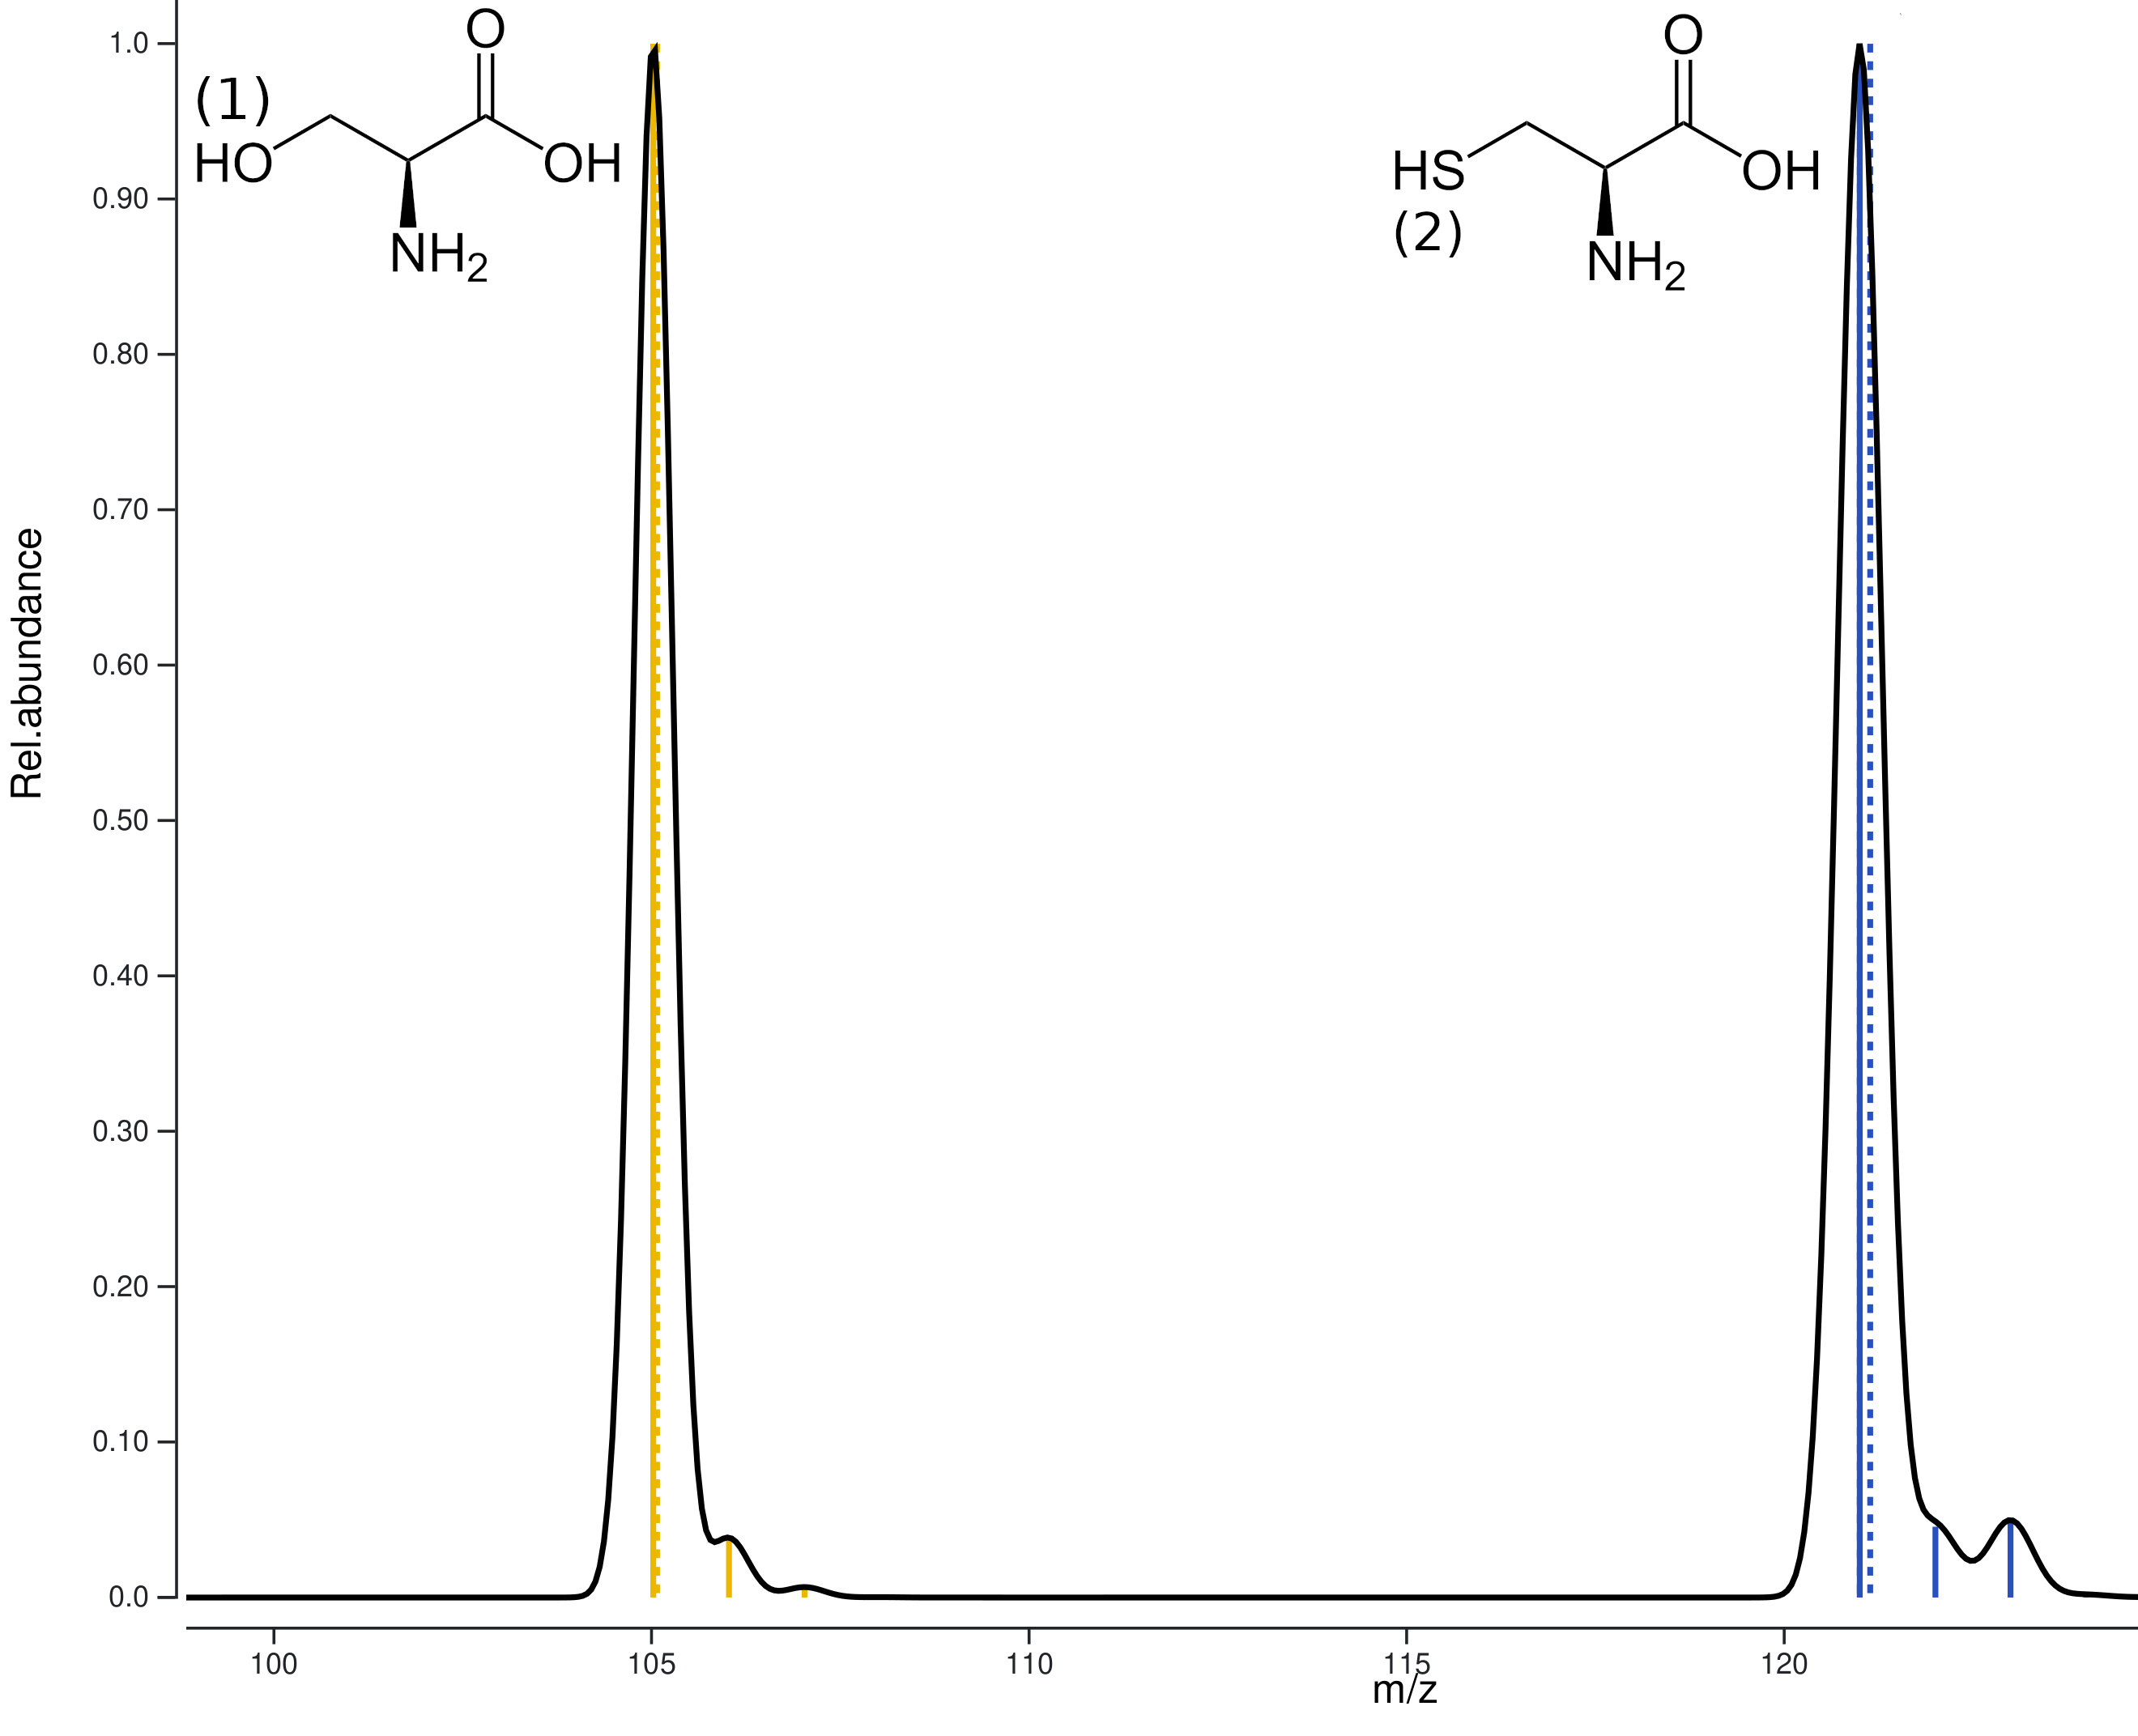
\includegraphics[width=0.75\textwidth]{./Resources/Simulated_Mass_Spectrum.png}
   \centering
   \caption{Computergeneriertes Massenspektrum von der Aminosäure \emph{Serin} (1) und \emph{Cystesin} (2). Peak von \emph{Serin} liegt bei 105; bei \emph{Systesin} um 121. y: relative Häufigkeit}
\end{figure}

Die Maxima werden \gerquot{Peaks} genannt und sind für eine Aminosäure an charakteristischer Position auf der $ x $-Achse. Obwohl sich die beiden Aminosäuren in der Abbildung \ref{fig:Sim_Mass_Spec} nur durch ein Atom unterscheiden (das linke Sauerstoffatom wurde durch ein Schwefelatom ersetzt) sind deren Massenspektren auf der $ x $-Achse weit voneinander entfernt und machen die beiden Aminosäuren dadurch sicher unterscheidbar.\\

Bei einzelnen Aminosäuren funktioniert die MS zuverlässig; bei Peptiden allerdings steht man vor dem Problem, dass das Massenspektrum unübersichtlicher wird und auch Peaks, die von Hintergrundrauschen stammen, schwerer herausgefiltert werden können. Abhilfe schafft hier die Tandem-Massenspektrometrie.

\subsection{Tandem-Massenspektrometrie (MS/MS)}\label{ss:Tandem_MS}
Bei der Tandem-Massenspektrometrie (MS/MS oder MS2) werden zwei MS Vorgänge hintereinander mit einer Probe durchgeführt. Die erste MS dient dazu Ionen aus einem bestimmten \massCharge Bereich auswählbar zu machen. Es entspricht also quasi einer Form der Filterung.

Vor der 2. MS werden die ausgewählten Reste einer Fragmentierung unterzogen. Bei einer Fragmentierung führt man Energie zu mit dem Ziel, dass die Ionen zerfallen und sog. Fragment-Ionen bilden. Diese Fragment-Ionen werden dann auf dem Massenspektrum nach der 2. MS sichtbar gemacht.

Fragment-Ionen sind kleiner als die ursprünglichen Ionen. So kann die 2. MS mit einer höheren Selektivität durchgeführt werden, welches Peaks durch Hintergrundrauschen verringert. Auch lassen sich Ionen besser identifizieren, die ein sehr ähnliches \massCharge-Verhältnis besitzen. Nach der 2. MS liegt eine Fülle an Fragment-Ionen-Peaks vor, aus denen sich die ursprünglichen Strukturinformationen ableiten lassen, da Ionen in spezifische Fragmente zerfallen \cite{Gross2013}. Zusammengefasst kann man sagen, dass das MS/MS Verfahren Ergebnisse höherer Güte erzeugt im Vergleich zur einfachen MS.

\section{De-Novo-Peptidsequenzierung mit \emph{pNovo+}}\label{s:pNovoPlusSeq}
Die \emph{pNovo+} Methode ist eine \gls{gls:DeNovo}, die mit einem \gls{gls:SpecGraph}en für die Auswertung der MS2-Spektren arbeitet und eine Erweiterung des \emph{pNovo} Verfahren darstellt \cite{pNovo}. Der Hauptansatz ist, dass zwei MS/MS Durchläufe mit jeweils verschiedenen Fragmentierungsmethoden\footnote{\emph{pNovo+} verwendet die higher energy
collisional dissociation (HCD) und die electron transfer dissociation (ETD) Fragmentierungsmethoden.} durchgeführt werden. Durch die Wahl einer anderen Fragmentierungsmethode ändert sich auch das MS2-Spektrum. Wenn nun Fragmentierungsmethoden verwendet werden, die möglichst komplementäre Spektren erzeugen, dann lässt sich durch das Zusammenführen der beiden MS2-Spektren die Qualität der Ergebnisse verbessern. Zum Beispiel lassen sich dadurch viele Peaks, die vom Hintergrundrauschen stammen, entfernen.

Für die Ermittlung der Sequenz eines Peptides wird zunächst ein Spektrums-Graph gebildet \dashAndSpace in Form eines DAG (directed acyclic graph). In diesem Graphen wird dann der längste Pfad bei gegebenen Start- und Endknoten berechnet. Die Reihenfolge der Knoten, die im längsten Pfad durchlaufen werden, stellt dann die Peptidsequenz dar.

\subsection{Vorverarbeitung der MS2-Spektren}\label{ss:Vorverarbeitung}
Bevor aus den MS2-Spektren der Spektrums-Graph gebildet werden kann, müssen die Daten vorverarbeitet werden. Für die Auswertung ist es von entscheidener Bedeutung, dass möglichst wenig Peaks verwendet werden, die vom Hintergrundrauschen stammen. Im weiteren Verlauf werden an einem exemplarischen MS2-Spektrum die Verarbeitungsschritte dargestellt.\\

Der erste Schritt ist das Verwenden des natürlichen Logarithmus der Intensitäten. Die Idee dabei ist, dass Hintergrundrauschen nicht überpriorisiert wird.

\begin{figure}[H]
   \centering
   \begin{minipage}[t]{.45\linewidth}
      \centering
      \begin{tikzpicture}[scale=\tikzScale, baseline=(current bounding box.center)]
         \draw [<->,thick] (0,\yAxisHeight) node (yaxis) [above] {\yAxisUnit}
         |- (\xAxisLength,0) node (xaxis) [right] {\xAxisUnit};
\draw[thick] (0.2, 0.0) -- (0.2, 2.3);
\draw[thick] (0.382, 0.0) -- (0.382, 1.7);
\draw[thick] (0.476, 0.0) -- (0.476, 2.7);
\draw[thick] (0.456, 0.0) -- (0.456, 1.8);
\draw[thick] (0.6859999999999999, 0.0) -- (0.6859999999999999, 2.7);
\draw[thick] (0.6839999999999999, 0.0) -- (0.6839999999999999, 1.8);
\draw[thick] (0.752, 0.0) -- (0.752, 1.1);
\draw[thick] (0.8200000000000001, 0.0) -- (0.8200000000000001, 2.2);
\draw[thick] (1.076, 0.0) -- (1.076, 1.5);
\draw[thick] (1.16, 0.0) -- (1.16, 1.9);
\draw[thick] (1.2120000000000002, 0.0) -- (1.2120000000000002, 2.0);
\draw[thick] (1.28, 0.0) -- (1.28, 1.9);
\draw[thick] (1.452, 0.0) -- (1.452, 1.3);
\draw[thick] (1.426, 0.0) -- (1.426, 1.9);
\draw[thick] (1.548, 0.0) -- (1.548, 1.9);
\draw[thick] (1.6740000000000002, 0.0) -- (1.6740000000000002, 1.5);
\draw[thick] (1.788, 0.0) -- (1.788, 2.5);
\draw[thick] (1.856, 0.0) -- (1.856, 2.3);
\draw[thick] (2.036, 0.0) -- (2.036, 1.7);
\draw[thick] (2.142, 0.0) -- (2.142, 1.6);
\draw[thick] (2.2520000000000002, 0.0) -- (2.2520000000000002, 2.0);
\draw[thick] (2.386, 0.0) -- (2.386, 1.6);
\draw[thick] (2.488, 0.0) -- (2.488, 2.9);
\draw[thick] (2.4739999999999998, 0.0) -- (2.4739999999999998, 2.7);
\draw[thick] (2.504, 0.0) -- (2.504, 2.0);
\draw[thick] (2.682, 0.0) -- (2.682, 2.0);
\draw[thick] (2.702, 0.0) -- (2.702, 2.5);
\draw[thick] (2.9259999999999997, 0.0) -- (2.9259999999999997, 2.8);
\draw[thick] (3.024, 0.0) -- (3.024, 2.4);
\draw[thick] (3.096, 0.0) -- (3.096, 1.8);
\draw[thick] (3.244, 0.0) -- (3.244, 2.6);
\draw[thick] (3.362, 0.0) -- (3.362, 1.9);
\draw[thick] (3.46, 0.0) -- (3.46, 2.3);
\draw[thick] (3.516, 0.0) -- (3.516, 1.1);
\draw[thick] (3.584, 0.0) -- (3.584, 1.8);
\draw[thick] (3.652, 0.0) -- (3.652, 2.0);
\draw[thick] (3.838, 0.0) -- (3.838, 1.5);
\draw[thick] (3.8819999999999997, 0.0) -- (3.8819999999999997, 2.6);
\draw[thick] (4.088, 0.0) -- (4.088, 2.6);
\draw[thick] (4.046, 0.0) -- (4.046, 1.1);
\draw[thick] (4.167999999999999, 0.0) -- (4.167999999999999, 2.0);
\draw[thick] (4.266, 0.0) -- (4.266, 2.4);
\draw[thick] (4.38, 0.0) -- (4.38, 1.1);
\draw[thick] (4.456, 0.0) -- (4.456, 2.2);
\draw[thick] (4.644, 0.0) -- (4.644, 2.6);
\draw[thick] (4.675999999999999, 0.0) -- (4.675999999999999, 2.5);
\draw[thick] (4.898000000000001, 0.0) -- (4.898000000000001, 1.2);
   \end{tikzpicture}%
   \end{minipage}%
   \textbf{$\rightarrow$} 
   \begin{minipage}[t]{.45\linewidth}
      \centering
      \begin{tikzpicture}[scale=\tikzScale, baseline=(current bounding box.center)]
      \draw [<->,thick] (0,\yAxisHeight) node (yaxis) [above] {\yAxisUnit}
      |- (\xAxisLength,0) node (xaxis) [right] {\xAxisUnit};
\draw[thick] (0.2, 0.0) -- (0.2, {ln(2.3)});
\draw[thick] (0.382, 0.0) -- (0.382, {ln(1.7)});
\draw[thick] (0.476, 0.0) -- (0.476, {ln(2.7)});
\draw[thick] (0.456, 0.0) -- (0.456, {ln(1.8)});
\draw[thick] (0.6859999999999999, 0.0) -- (0.6859999999999999, {ln(2.7)});
\draw[thick] (0.6839999999999999, 0.0) -- (0.6839999999999999, {ln(1.8)});
\draw[thick] (0.752, 0.0) -- (0.752, {ln(1.1)});
\draw[thick] (0.8200000000000001, 0.0) -- (0.8200000000000001, {ln(2.2)});
\draw[thick] (1.076, 0.0) -- (1.076, {ln(1.5)});
\draw[thick] (1.16, 0.0) -- (1.16, {ln(1.9)});
\draw[thick] (1.2120000000000002, 0.0) -- (1.2120000000000002, {ln(2.0)});
\draw[thick] (1.28, 0.0) -- (1.28, {ln(1.9)});
\draw[thick] (1.452, 0.0) -- (1.452, {ln(1.3)});
\draw[thick] (1.426, 0.0) -- (1.426, {ln(1.9)});
\draw[thick] (1.548, 0.0) -- (1.548, {ln(1.9)});
\draw[thick] (1.6740000000000002, 0.0) -- (1.6740000000000002, {ln(1.5)});
\draw[thick] (1.788, 0.0) -- (1.788, {ln(2.5)});
\draw[thick] (1.856, 0.0) -- (1.856, {ln(2.3)});
\draw[thick] (2.036, 0.0) -- (2.036, {ln(1.7)});
\draw[thick] (2.142, 0.0) -- (2.142, {ln(1.6)});
\draw[thick] (2.2520000000000002, 0.0) -- (2.2520000000000002, {ln(2.0)});
\draw[thick] (2.386, 0.0) -- (2.386, {ln(1.6)});
\draw[thick] (2.488, 0.0) -- (2.488, {ln(2.9)});
\draw[thick] (2.4739999999999998, 0.0) -- (2.4739999999999998, {ln(2.7)});
\draw[thick] (2.504, 0.0) -- (2.504, {ln(2.0)});
\draw[thick] (2.682, 0.0) -- (2.682, {ln(2.0)});
\draw[thick] (2.702, 0.0) -- (2.702, {ln(2.5)});
\draw[thick] (2.9259999999999997, 0.0) -- (2.9259999999999997, {ln(2.8)});
\draw[thick] (3.024, 0.0) -- (3.024, {ln(2.4)});
\draw[thick] (3.096, 0.0) -- (3.096, {ln(1.8)});
\draw[thick] (3.244, 0.0) -- (3.244, {ln(2.6)});
\draw[thick] (3.362, 0.0) -- (3.362, {ln(1.9)});
\draw[thick] (3.46, 0.0) -- (3.46, {ln(2.3)});
\draw[thick] (3.516, 0.0) -- (3.516, {ln(1.1)});
\draw[thick] (3.584, 0.0) -- (3.584, {ln(1.8)});
\draw[thick] (3.652, 0.0) -- (3.652, {ln(2.0)});
\draw[thick] (3.838, 0.0) -- (3.838, {ln(1.5)});
\draw[thick] (3.8819999999999997, 0.0) -- (3.8819999999999997, {ln(2.6)});
\draw[thick] (4.088, 0.0) -- (4.088, {ln(2.6)});
\draw[thick] (4.046, 0.0) -- (4.046, {ln(1.1)});
\draw[thick] (4.167999999999999, 0.0) -- (4.167999999999999, {ln(2.0)});
\draw[thick] (4.266, 0.0) -- (4.266, {ln(2.4)});
\draw[thick] (4.38, 0.0) -- (4.38, {ln(1.1)});
\draw[thick] (4.456, 0.0) -- (4.456, {ln(2.2)});
\draw[thick] (4.644, 0.0) -- (4.644, {ln(2.6)});
\draw[thick] (4.675999999999999, 0.0) -- (4.675999999999999, {ln(2.5)});
\draw[thick] (4.898000000000001, 0.0) -- (4.898000000000001, {ln(1.2)});
      \end{tikzpicture}
      \end{minipage}
      \caption{Anwendung des $ ln $ auf einem exemplarischen MS2-Spektrum.}
\end{figure}

Für das Verständnis des nächsten Schrittes muss man sich in Erinnerung rufen, dass eine gleiche Aminosäure keineswegs immer die gleiche Masse hat. Durch Isotope existiert eine gewisse \gerquot{Massenbandbreite} für ein und dieselbe Aminosäure. MS Systeme sind heute so genau, dass sie diese Differenzen erkennen. Dies hat den ungewollten Effekt, dass mehrere Peaks zu einer Aminosäure gehören können \cite{IsotopicDistributionMS}. Gleichzeitig können die \gerquot{Massenbandbreiten} zweier Aminosäuren sich überschneiden, sodass im ungünstigen Fall zwei Peaks kaum unterscheidbar nebeneinander liegen.\\

Eine Möglichkeit mit dieser Problematik umzugehen ist die Verwendung der monoisotopischen Masse. Die monoisotopische Masse ist die \gerquot{[...] exact mass of the most abundant naturally occurring stable isotope determined relative to the mass of 12 C, which is assigned the exact value of 12.0000.} \cite{MonoisotopicMass}. Ohne dabei jetzt tiefer ins Detail zu gehen kann man sagen, dass alle Peaks, deren Intensität mit einer möglichen monoisotopischen Masse übereinstimmen, auf jeden Fall einer Aminosäure entsprechen und (höchstwahrscheinlich)\footnote{Natürlich ist es möglich, dass das Rauschen zufällig einer monoisotopischen Masse entspricht. Die Wahrscheinlichkeit dafür ist allerdings sehr gering.} kein Hintergrundrauschen sind \cite{MassDefectMS}. Diese Peaks bekommen eine sogennante \emph{charge state}.\\

Der Algorithmus verwendet die \emph{charge state} Peaks als Ausganspunkte für weitere Berechnungen. Wenn die \massCharge Differenz zu einem anderen Peak einem Peptidfragment entspricht, dann stammt dieser Peak höchstwahrscheinlich von einem Fragment. Insgesamt werden damit die relevanten Peptidfragmente herausgeholt. Abbildung \ref{MonoisotopicMassFiltering} zeigt das Ergebnis nach den beiden zuvor genannten Schritten.

\begin{figure}[H]\label{MonoisotopicMassFiltering}
   \centering
   \begin{minipage}[t]{.45\linewidth}
      \centering
      \begin{tikzpicture}[scale=\tikzScale, baseline=(current bounding box.center)]
         \draw [<->,thick] (0,\yAxisHeight) node (yaxis) [above] {\yAxisUnit}
         |- (\xAxisLength,0) node (xaxis) [right] {\xAxisUnit};
\draw[thick] (0.2, 0.0) -- (0.2, {ln(2.3)});
\draw[color=blue!85!,opacity=.55,thick] (0.382, 0.0) -- (0.382, {ln(1.7)});
\draw[color=blue!85!,opacity=.55,thick] (0.476, 0.0) -- (0.476, {ln(2.7)});
\draw[color=magenta,thick] (0.456, 0.0) -- (0.456, {ln(1.8)});
\draw[color=blue!85!,opacity=.55,thick] (0.6859999999999999, 0.0) -- (0.6859999999999999, {ln(2.7)});
\draw[color=blue!85!,opacity=.55,thick] (0.6839999999999999, 0.0) -- (0.6839999999999999, {ln(1.8)});
\draw[thick] (0.752, 0.0) -- (0.752, {ln(1.1)});
\draw[thick] (0.8200000000000001, 0.0) -- (0.8200000000000001, {ln(2.2)});
\draw[thick] (1.076, 0.0) -- (1.076, {ln(1.5)});
\draw[thick] (1.16, 0.0) -- (1.16, {ln(1.9)});
\draw[thick] (1.2120000000000002, 0.0) -- (1.2120000000000002, {ln(2.0)});
\draw[thick] (1.28, 0.0) -- (1.28, {ln(1.9)});
\draw[color=blue!85!,opacity=.55,thick] (1.452, 0.0) -- (1.452, {ln(1.3)});
\draw[color=blue!85!,opacity=.55,thick] (1.426, 0.0) -- (1.426, {ln(1.9)});
\draw[color=magenta,thick] (1.548, 0.0) -- (1.548, {ln(1.9)});
\draw[color=blue!85!,opacity=.55,thick] (1.6740000000000002, 0.0) -- (1.6740000000000002, {ln(1.5)});
\draw[color=blue!85!,opacity=.55,thick] (1.788, 0.0) -- (1.788, {ln(2.5)});
\draw[thick] (1.856, 0.0) -- (1.856, {ln(2.3)});
\draw[thick] (2.036, 0.0) -- (2.036, {ln(1.7)});
\draw[thick] (2.142, 0.0) -- (2.142, {ln(1.6)});
\draw[thick] (2.2520000000000002, 0.0) -- (2.2520000000000002, {ln(2.0)});
\draw[thick] (2.386, 0.0) -- (2.386, {ln(1.6)});
\draw[color=blue!85!,opacity=.55,thick] (2.488, 0.0) -- (2.488, {ln(2.9)});
\draw[thick] (2.4739999999999998, 0.0) -- (2.4739999999999998, {ln(2.7)});
\draw[color=blue!85!,opacity=.55,thick] (2.504, 0.0) -- (2.504, {ln(2.0)});
\draw[color=magenta,thick] (2.682, 0.0) -- (2.682, {ln(2.0)});
\draw[color=blue!85!,opacity=.55,thick] (2.702, 0.0) -- (2.702, {ln(2.5)});
\draw[thick] (2.9259999999999997, 0.0) -- (2.9259999999999997, {ln(2.8)});
\draw[thick] (3.024, 0.0) -- (3.024, {ln(2.4)});
\draw[thick] (3.096, 0.0) -- (3.096, {ln(1.8)});
\draw[thick] (3.244, 0.0) -- (3.244, {ln(2.6)});
\draw[thick] (3.362, 0.0) -- (3.362, {ln(1.9)});
\draw[color=blue!85!,opacity=.55,thick] (3.46, 0.0) -- (3.46, {ln(2.3)});
\draw[color=blue!85!,opacity=.55,thick] (3.516, 0.0) -- (3.516, {ln(1.1)});
\draw[color=blue!85!,opacity=.55,thick] (3.584, 0.0) -- (3.584, {ln(1.8)});
\draw[color=magenta,thick] (3.652, 0.0) -- (3.652, {ln(2.0)});
\draw[color=blue!85!,opacity=.55,thick] (3.838, 0.0) -- (3.838, {ln(1.5)});
\draw[color=blue!85!,opacity=.55,thick] (3.8819999999999997, 0.0) -- (3.8819999999999997, {ln(2.6)});
\draw[thick] (4.088, 0.0) -- (4.088, {ln(2.6)});
\draw[thick] (4.046, 0.0) -- (4.046, {ln(1.1)});
\draw[thick] (4.167999999999999, 0.0) -- (4.167999999999999, {ln(2.0)});
\draw[thick] (4.266, 0.0) -- (4.266, {ln(2.4)});
\draw[color=blue!85!,opacity=.55,thick] (4.38, 0.0) -- (4.38, {ln(1.1)});
\draw[color=blue!85!,opacity=.55,thick] (4.456, 0.0) -- (4.456, {ln(2.2)});
\draw[color=magenta,thick] (4.644, 0.0) -- (4.644, {ln(2.6)});
\draw[color=blue!85!,opacity=.55,thick] (4.675999999999999, 0.0) -- (4.675999999999999, {ln(2.5)});
\draw[color=blue!85!,opacity=.55,thick] (4.898000000000001, 0.0) -- (4.898000000000001, {ln(1.2)});
   \end{tikzpicture}%
   \end{minipage}%
   \textbf{$\rightarrow$} 
   \begin{minipage}[t]{.45\linewidth}
      \centering
      \begin{tikzpicture}[scale=\tikzScale, baseline=(current bounding box.center)]
      \draw [<->,thick] (0,\yAxisHeight) node (yaxis) [above] {\yAxisUnit}
      |- (\xAxisLength,0) node (xaxis) [right] {\xAxisUnit};
\draw[color=blue!85!,opacity=.55,thick] (0.382, 0.0) -- (0.382, {ln(1.7)});
\draw[color=blue!85!,opacity=.55,thick] (0.476, 0.0) -- (0.476, {ln(2.7)});
\draw[color=magenta,thick] (0.456, 0.0) -- (0.456, {ln(1.8)});
\draw[color=blue!85!,opacity=.55,thick] (0.6859999999999999, 0.0) -- (0.6859999999999999, {ln(2.7)});
\draw[color=blue!85!,opacity=.55,thick] (0.6839999999999999, 0.0) -- (0.6839999999999999, {ln(1.8)});
\draw[color=blue!85!,opacity=.55,thick] (1.452, 0.0) -- (1.452, {ln(1.3)});
\draw[color=blue!85!,opacity=.55,thick] (1.426, 0.0) -- (1.426, {ln(1.9)});
\draw[color=magenta,thick] (1.548, 0.0) -- (1.548, {ln(1.9)});
\draw[color=blue!85!,opacity=.55,thick] (1.6740000000000002, 0.0) -- (1.6740000000000002, {ln(1.5)});
\draw[color=blue!85!,opacity=.55,thick] (1.788, 0.0) -- (1.788, {ln(2.5)});
\draw[color=blue!85!,opacity=.55,thick] (2.488, 0.0) -- (2.488, {ln(2.9)});
\draw[color=blue!85!,opacity=.55,thick] (2.504, 0.0) -- (2.504, {ln(2.0)});
\draw[color=magenta,thick] (2.682, 0.0) -- (2.682, {ln(2.0)});
\draw[color=blue!85!,opacity=.55,thick] (2.702, 0.0) -- (2.702, {ln(2.5)});
\draw[color=blue!85!,opacity=.55,thick] (3.46, 0.0) -- (3.46, {ln(2.3)});
\draw[color=blue!85!,opacity=.55,thick] (3.516, 0.0) -- (3.516, {ln(1.1)});
\draw[color=blue!85!,opacity=.55,thick] (3.584, 0.0) -- (3.584, {ln(1.8)});
\draw[color=magenta,thick] (3.652, 0.0) -- (3.652, {ln(2.0)});
\draw[color=blue!85!,opacity=.55,thick] (3.838, 0.0) -- (3.838, {ln(1.5)});
\draw[color=blue!85!,opacity=.55,thick] (3.8819999999999997, 0.0) -- (3.8819999999999997, {ln(2.6)});
\draw[color=blue!85!,opacity=.55,thick] (4.38, 0.0) -- (4.38, {ln(1.1)});
\draw[color=blue!85!,opacity=.55,thick] (4.456, 0.0) -- (4.456, {ln(2.2)});
\draw[color=magenta,thick] (4.644, 0.0) -- (4.644, {ln(2.6)});
\draw[color=blue!85!,opacity=.55,thick] (4.675999999999999, 0.0) -- (4.675999999999999, {ln(2.5)});
\draw[color=blue!85!,opacity=.55,thick] (4.898000000000001, 0.0) -- (4.898000000000001, {ln(1.2)});
      \end{tikzpicture}
      \end{minipage}
      \caption{Entfernen von Peaks, die keiner monoisotopischen Masse entsprechen oder benachbart mit einer Differenz von einem Fragment-Ion sind.}
\end{figure}

Tatsächlich ist die Verarbeitung an dieser Stelle noch etwas komplexer. So existieren auch noch sogenannte \emph{isotopic cluster}\footnote{Definition eines \emph{isotopic cluster} nach IUPAC: \gerquot{Group of peaks representing ions of the same elemental composition, but different isotopic compositions.} \cite[1556]{IUPACDefinitions}}, die gesondert verarbeitet werden. Für das grundsätzliche Prinzip ist dieses Detail allerdings weniger relevant.\\

Im letzten Vorberarbeitungsschritt werden Peaks aus einem irrelevanten \massCharge Bereich entfernt und naheliegende Peaks werden zusammengefasst, indem der Mittelwert sowol des \massCharge Wertes als auch der der Intensität besimmt wird. Üblicherweise liegt der Bereich für das Zusammenfassen bei $ +- 20 ppm $.

\begin{figure}[H]
   \centering
   \begin{minipage}[t]{.45\linewidth}
      \centering
      \begin{tikzpicture}[scale=\tikzScale, baseline=(current bounding box.center)]
         \draw [<->,thick] (0,\yAxisHeight) node (yaxis) [above] {\yAxisUnit}
         |- (\xAxisLength,0) node (xaxis) [right] {\xAxisUnit};
\draw[thick] (0.382, 0.0) -- (0.382, {ln(1.7)});
\draw[thick] (0.476, 0.0) -- (0.476, {ln(2.7)});
\draw[thick] (0.456, 0.0) -- (0.456, {ln(1.8)});
\draw[thick] (0.6859999999999999, 0.0) -- (0.6859999999999999, {ln(2.7)});
\draw[thick] (0.6839999999999999, 0.0) -- (0.6839999999999999, {ln(1.8)});
\draw[color=red,thick] (1.452, 0.0) -- (1.452, {ln(1.3)});
\draw[color=red,thick] (1.426, 0.0) -- (1.426, {ln(1.9)});
\draw[thick] (1.548, 0.0) -- (1.548, {ln(1.9)});
\draw[thick] (1.6740000000000002, 0.0) -- (1.6740000000000002, {ln(1.5)});
\draw[thick] (1.788, 0.0) -- (1.788, {ln(2.5)});
\draw[color=red,thick] (2.488, 0.0) -- (2.488, {ln(2.9)});
\draw[color=red,thick] (2.504, 0.0) -- (2.504, {ln(2.0)});
\draw[color=red,thick] (2.682, 0.0) -- (2.682, {ln(2.0)});
\draw[color=red,thick] (2.702, 0.0) -- (2.702, {ln(2.5)});
\draw[thick] (3.46, 0.0) -- (3.46, {ln(2.3)});
\draw[thick] (3.516, 0.0) -- (3.516, {ln(1.1)});
\draw[thick] (3.584, 0.0) -- (3.584, {ln(1.8)});
\draw[thick] (3.652, 0.0) -- (3.652, {ln(2.0)});
\draw[color=red,thick] (3.838, 0.0) -- (3.838, {ln(1.5)});
\draw[color=red,thick] (3.8819999999999997, 0.0) -- (3.8819999999999997, {ln(2.6)});
\draw[thick] (4.38, 0.0) -- (4.38, {ln(1.1)});
\draw[thick] (4.456, 0.0) -- (4.456, {ln(2.2)});
\draw[thick] (4.644, 0.0) -- (4.644, {ln(2.6)});
\draw[thick] (4.675999999999999, 0.0) -- (4.675999999999999, {ln(2.5)});
\draw[thick] (4.898000000000001, 0.0) -- (4.898000000000001, {ln(1.2)});

\fill[red!25!,opacity=.25] (0,0) rectangle (1,\yAxisHeight-\axisColorOffset);
         \fill[red!25!,opacity=.25] (\xAxisLength-1,0) rectangle (\xAxisLength-\axisColorOffset,\yAxisHeight-\axisColorOffset);
         \fill[green!25!,opacity=.25] (1,0) rectangle (\xAxisLength-1,\yAxisHeight-\axisColorOffset);
   \end{tikzpicture}%
   \end{minipage}%
   \textbf{$\rightarrow$} 
   \begin{minipage}[t]{.45\linewidth}
      \centering
      \begin{tikzpicture}[scale=\tikzScale, baseline=(current bounding box.center)]
      \draw [<->,thick] (0,\yAxisHeight) node (yaxis) [above] {\yAxisUnit}
      |- (\xAxisLength,0) node (xaxis) [right] {\xAxisUnit};
%\draw[color=red,thick] (1.452, 0.0) -- (1.452, {ln(1.3)});
%\draw[color=red,thick] (1.426, 0.0) -- (1.426, {ln(1.9)});
\draw[color=red,ultra thick] ({(1.452+1.426)/2}, 0.0) -- ({(1.452+1.426)/2}, {(ln(1.3)+ln(1.9))/2});

\draw[thick] (1.548, 0.0) -- (1.548, {ln(1.9)});
\draw[thick] (1.6740000000000002, 0.0) -- (1.6740000000000002, {ln(1.5)});
\draw[thick] (1.788, 0.0) -- (1.788, {ln(2.5)});

%\draw[color=red,thick] (2.488, 0.0) -- (2.488, {ln(2.9)});
%\draw[color=red,thick] (2.504, 0.0) -- (2.504, {ln(2.0)});
\draw[color=red,ultra thick] ({(2.488+2.504)/2}, 0.0) -- ({(2.488+2.504)/2}, {(ln(2.9)+ln(2.0))/2});

%\draw[color=red,thick] (2.682, 0.0) -- (2.682, {ln(2.0)});
%\draw[color=red,thick] (2.702, 0.0) -- (2.702, {ln(2.5)});
\draw[color=red,ultra thick] ({(2.682+2.702)/2}, 0.0) -- ({(2.682+2.702)/2}, {(ln(2.0+ln(2.5))/2});

\draw[thick] (3.46, 0.0) -- (3.46, {ln(2.3)});
\draw[thick] (3.516, 0.0) -- (3.516, {ln(1.1)});
\draw[thick] (3.584, 0.0) -- (3.584, {ln(1.8)});
\draw[thick] (3.652, 0.0) -- (3.652, {ln(2.0)});

%\draw[color=red,thick] (3.838, 0.0) -- (3.838, {ln(1.5)});
%\draw[color=red,thick] (3.8819999999999997, 0.0) -- (3.8819999999999997,{ln(2.6)});
\draw[color=red,ultra thick] ({(3.838+3.8819999999999997)/2}, 0.0) -- ({(3.838+3.8819999999999997)/2}, {(ln(1.5)+ln(2.6))/2});

\fill[red!25!,opacity=.25] (0,0) rectangle (1,\yAxisHeight-\axisColorOffset);
         \fill[red!25!,opacity=.25] (\xAxisLength-1,0) rectangle (\xAxisLength-\axisColorOffset,\yAxisHeight-\axisColorOffset);
         \fill[green!25!,opacity=.25] (1,0) rectangle (\xAxisLength-1,\yAxisHeight-\axisColorOffset);
      \end{tikzpicture}
      \end{minipage}
      \caption{Entfernen von Peaks aus einem irrelevanten \massCharge Bereich und zusammenfassen naheliegender Peaks. Rot markierte Peaks sind jene, die zusammengefasst werden.}
\end{figure}

\subsection{Bildung eines Spektrums-Graphen}\label{ss:BildungSpekGraph}
Der Spektrums-Graph wird aus einem vorverarbeiteten MS2-Spektrum (siehe Kapitel: \ref{ss:Vorverarbeitung}) gebildet. Im initialen Zustand werden die Peaks als Knoten interpretiert. Dazu kommt ein Start- und Endknoten. Jedem Knoten wird eine Masse zugeordet; im initialen Zustand bekommt der Startknoten die Masse 0 und der Endknoten die Masse des vorherigen Knotens minus der Masse des Wassers ($ 18,02 $). Die Masse der übrigen Knoten entsprechen ihren jeweils korrespondierenden \massCharge Wert. Die gerichteten Kanten werden zwischen einem Knotenpaar hinzugefügt, wenn die Differenz deren Masse gleich ist mit der Masse von ein oder zwei Aminosäuren.

\subsection{Identifikation der Aminosäuresequenz}
Der gebildete DAG kann mit klassischen Algorithmen, die den längsten Pfad suchen, durchlaufen werden. Bezogen auf die Graphentheorie entspricht die Ermittlung der Aminosäurensequenz dem Suchen eines bestimmten Pfades \dashAndSpace und nicht nach irgendeinem Pfad. Daher muss der Algorithmus mittels einer Breitensuche arbeiten, um alle möglichen Pfade zu bestimmen.

In aller Regel wird es mehrere Pfade geben. Bestimmte Sequenzen sind wahrscheinlicher als andere. So sind Pfade mit Kanten, die wegen der Massendifferenz von genau einer Aminosäure gebildet wurden, wahrscheinlicher \cite{pNovoPlus}. Alle Pfade bekommen mittels einer Scoring-Funktion einen Wert zugewiesen. Der Pfad mit dem höchsten Scoring-Wert ist wahrscheinlich das richtige Ergebnis. Die Scoring-Funktion berücksichtigt unter anderem wie viele Fragmente, die einer bestimmten Aminosäure zugeordet werden können, im MS2-Spektrum vorhanden sind \cite{pNovo}. Die Sequenz mit dem höchsten Scoring-Wert ist das Endergebnis.

\section{De-Novo-Peptidsequenzierung mit \emph{Open-pNovo}}\label{s:OpenpNovoSeq}
Bei Proteinen können posttranslationale Proteinmodifikationen (PTM) auftreten. PTMs sind Ereignisse, bei denen sich Änderungen im Protein einstellen \cite{Mann2003}; teilweise sind die Änderungen von einer Zelle erwünscht \dashAndSpace teilweise stammen sie aber auch zum Beispiel von unerwünschten Wechselwirkungen nebeneinanderliegenden Aminosäuren. Ein Teil dieser PTMs führen zu einer Änderung der Aminosäuresequenz. Dies ist für die \gls{gls:DeNovo} nicht weiter problematisch, da sowieso ohne eine Datenbank gearbeitet wird, sodass solche PTMs nicht einmal auffallen würden. Andere PTMs hingegen haben die Auswirkung, dass Stoffe gebildet werden, die nicht mehr zu der Gruppe der proteinogenen Aminosäuren gehören. Proteinogene Aminosäuren sind jene Aminosäuren, die für den Bau von Proteinen verwendet werden. Der Effekt ist also, dass Stoffe (oder deren Fragmente) bei einem Massenspektrum angezeigt werden, die kein Teil eines Peptids sein können. Bei der Sequenzierung von Peptidfragmenten muss dies daher berücksichtigt werden.
Wenn im weiteren Verlauf von PTMs gesprochen wird, dann sind solche gemeint, die für die \gls{gls:DeNovo} relevant sind.

Open-pNovo ist ein \gls{gls:DeNovo}sverfahren, welches auf pNovo+ Tool aufbaut und versucht die Problematik mit den PTMs zu lösen.

\subsection{PTMs im konstruierten DAG}
Die Konvertierung eines MS2-Spektrums läuft bis zum DAG analog ab wie in den Kapiteln \ref{ss:Vorverarbeitung} und \ref{ss:BildungSpekGraph} für pNovo+. Der Unterschied ist nun, dass es zwei Arten von Kanten gibt:

\begin{itemize}
   \item \gerquot{Normale} Kanten: Kanten, die gebildet werden, wie es bereits für \emph{pNovo+} gezeigt wurde. 
   \item \gerquot{Modifizierte} Kanten: Kanten, die zum Grahpen hinzugefügt werden, wenn die Massendifferenz zweier Knoten der Masse einer Aminosäure plus der Masse einer möglichen PTM-Änderung entspricht. 
\end{itemize}

Eine Liste aller PTMs in der Datenbank Unimod (sowohl relevante als auch nicht relevante) beinhaltet aktuell 1510 Einträge\footnote{Siehe: \url{https://www.ebi.ac.uk/ols/ontologies/unimod}} (Stand: 18.04.2022). Für die modifizierten Kanten gibt es insgesamt $ 1510 * 20 = 30200 $ mögliche Differenzen, wobei viele davon nicht relevante PTMs sind. Zum Vergleich: bei den normalen Kanten gibt es $ 20^2 = 400 $ mögliche Differenzen.

Die hohe Anzahl an Differenzen für modifizierte Kanten hat die Konsequenz, dass viele Knoten zufällig verbunden werden und dass dadurch die Genauigkeit der Ergebnisse abnimmt. Dieses Problem kann man durch eine geringere Liste an möglichen PTMs abfedern, allerdings mit einem Verlust  der Genauigkeit auf Seiten der PTMs. Es ist hier also eine Abwägung.

\subsection{Evaluierung von Open-pNovo}
Open-pNovo wurde sowohl auf drei realen als auch auf drei generierten Testdaten getestet. Tabelle \ref{tab:OpenPNovoResults} zeigt die Ergebnisse im Vergleich zu pNovo+ und zwei anderen Algorithmen. Die Datensätze enthielten die am häufigsten vorkommenden PTMs.

\begin{table}[H]
    \centering
    \begin{tabular}{l|c|c|c|c}
        \toprule
        \textbf{Testdatensätze} & \textbf{Open-pNovo+} & \textbf{pNovo+} & \textbf{PEAKS} & \textbf{Novor} \\
        \midrule
        Real (20259) & $76,3 \%$ & $68,5 \%$ & $65,8 \%$ & $39,9 \%$ \\
        Generiert (17877) & $77,8 \%$ & $0,6 \%$ & $0,5 \%$ & $0,2 \%$ \\
        \bottomrule
    \end{tabular}
    \newline
    \caption{Vergleich der durchschnittlichen richtigen \gls{gls:DeNovo} Peptidsequenzierungen von Open-pNovo und anderen Algorithmen \cite[650]{OpenPNovo}.}
    \label{tab:OpenPNovoResults}
\end{table}

Die enorm schlechten Ergebnisse der anderen Algorithmen bei den generierten Testdaten ist ein Nebeneffekt des Ziels bei der Testdatengenerierung. Denn diese wurden so ausgelegt, um die Grenzen von Open-pNovo+ zu ermitteln \cite[649]{OpenPNovo}. Eine Aussagekraft haben diese Ergebnisse also nicht. Allerdings auch bei realen Testdaten zeigt sich Open-pNovo als voll konkurrenzfähig gegenüber den anderen Algorithmen.

Noch besser zeigt sich Open-pNovo, wenn der Recall Wert betrachtet wird \dashAndSpace also die Anzahl an verschiedenen PSMs, die erkannt wurden. In diesem Fall ist der Abstand zu den anderen Algorithmen deutlich größer geworden.

\begin{table}[H]
    \centering
    \begin{tabular}{l|c|c|c|c}
        \toprule
        \textbf{Testdatensätze} & \textbf{Open-pNovo+} & \textbf{pNovo+} & \textbf{PEAKS} & \textbf{Novor} \\
        \midrule
        Real (5034) & $61,6 \%$ & $31,3 \%$ & $32,0 \%$ & $13,7 \%$ \\
        \bottomrule
    \end{tabular}
    \newline
    \caption{Vergleich der durchschnittlichen Recall Werte einer \gls{gls:DeNovo} Peptidsequenzierungen von Open-pNovo und anderen Algorithmen \cite[650]{OpenPNovo}.}
    \label{tab:OpenPNovoResultsRecall}
\end{table}

\subsection{Zusammenfassung}


% Die \gls{gls:DeNovo} nutzt die sogenannte \gls{gls:TMassSpek} für die Bestimmung der Peptidsequenz. Dabei wird die physikalische Eigenschaft ausgenutzt, dass jedes Atom bzw. jedes Molekül \dashAndSpace wenn es einer \gls{gls:Ionisation} unterzogen wurde \dashAndSpace ein charakteristisches \gls{gls:MassSpek} besitzt. Das \gls{gls:MassSpek} stellt also eine Art \gerquot{Fingerabdruck} eines Moleküls dar und macht dieses ermittelbar.

% U.U. eine Beispielgrafik eines Massenspektrums hinzufuegen ...

\subsubsection{\glsentrytext{gls:TMassSpek} bei größeren Molekülen}
Bei größeren Molekülen (wie einem Protein) führt die \gls{gls:Ionisation} dazu, dass das Molekül in kleinere spezifische Ionen zerfällt (sog. Fragmentierung). Die Fragmentierungsinformationen einer \gls{gls:DeNovo} sind meist unvollständig, da fehlende Daten bei einem Fragmentierungsschritt die Güte des Endergebnisses negativ beeinflusst. Dies wird insbesondere dann ein Problem, wenn unbekannte Änderungen in einer Peptidsequenz vorhanden sind.

Um dieses Problem zu verringern können unterschiedliche Techniken parallel eingesetzt werden, welche verschiedene Fragmente erzeugen und daher auch verschiedenartige \glspl{gls:MassSpek} zur Folge haben.\footnote{Konkret: Es wird sowohl das \gls{acr:HCD} als auch das \gls{acr:ETD} Verfahren angewendet.}

\subsection{Datenaufbereitung}
Typischerweise betrachtet man die sog. \gerquot{\glspl{gls:Peak}} in den \glspl{gls:MassSpek}. Jeder \gls{gls:Peak} stellt ein unterschiedliches Ion dar. Dazu kommen Messungenauigkeiten sowie Hintergrundrauschen. Durch die hohe Anzahl an möglichen Ionen kann nicht ohne weiteres differenziert werden, welcher der \glspl{gls:Peak} von welchen Ionen erzeugt wurden und welche nicht.

% Frage an Dominik: Ist hier eine einfache Auflistung an Techniken für die Datenaufbereitung besser?
Der Algorithmus für die Datenaufbereitung berechnet den natürlichen Logarithmus von den Intensitäten der \glspl{gls:Peak}, um Hintergrundrauschen und Messungenauigkeiten nicht überzupriorisieren. Zusätzlich dazu werden \glspl{gls:Peak}, die in einem Toleranzbereich nebeneinander liegen, zusammengefasst. Am Ende werden die \glspl{gls:Peak} entfernt, bei denen bekannt ist, dass es sich nicht um relevante Ionen handeln kann. (z.B. \glspl{gls:Peak} von Isotopen)

\begin{figure}[H]
   \centering
   \begin{minipage}[t]{.4\linewidth}
      \centering
      \begin{tikzpicture}[scale=\tikzScale, baseline=(current bounding box.center)]
         \draw [<->,thick] (0,2.75) node (yaxis) [above] {\yAxisUnit}
         |- (3,0) node (xaxis) [right] {\xAxisUnit};

         \draw[thick] (0.2,0) -- (0.2,1.1);
         \draw[thick] (0.3,0) -- (0.3,1.6);
         \draw[thick] (0.6,0) -- (0.6,1.7);
         \draw[thick] (0.8,0) -- (0.8,1.2);
         \draw[thick] (1.0,0) -- (1.0,1.1);

         \draw[color=red,thick] (1.2,0) -- (1.2,2.65);
         \draw[thick] (1.4,0) -- (1.4,1.4);
         \draw[thick] (1.6,0) -- (1.6,1.2);
         \draw[thick] (1.8,0) -- (1.8,1.3);
         \draw[thick] (2.0,0) -- (2.0,1.8);

         \draw[thick] (1.1,0) -- (1.1,2.0);
         \draw[color=red,thick] (0.35,0) -- (0.35,2.25);
         \draw[thick] (1.9,0) -- (1.9,1.4);
         \draw[color=red,thick] (2.2,0) -- (2.2,2.6);
         \draw[thick] (2.5,0) -- (2.5,1.25);

         \draw[thick] (2.7,0) -- (2.7,1.1);
         \foreach \x in {1,...,6}
         {
            \draw[thick] (1.2+\x*0.05,0) -- (1.2+\x*0.05,1.0+\x*0.15);
         }
      \end{tikzpicture}%
      % \subcaption{Exemplarische Rohdaten}
   \end{minipage}%
   \textbf{$\rightarrow$}
   \begin{minipage}[t]{.4\linewidth}
      \centering
      \begin{tikzpicture}[scale=\tikzScale, baseline=(current bounding box.center)]
         \draw [<->,thick] (0,2.75) node (yaxis) [above] {\yAxisUnit}
         |- (3,0) node (xaxis) [right] {\xAxisUnit};

         \draw[thick] (0.2,0) -- (0.2,{ln(1.1)});
         \draw[thick] (0.3,0) -- (0.3,{ln(1.6)});
         \draw[thick] (0.6,0) -- (0.6,{ln(1.7)});
         \draw[thick] (0.8,0) -- (0.8,{ln(1.2)});
         \draw[thick] (1.0,0) -- (1.0,{ln(1.1)});

         \draw[color=red,thick] (1.2,0) -- (1.2,{ln(2.65)});
         \draw[thick] (1.4,0) -- (1.4,{ln(1.4)});
         \draw[thick] (1.6,0) -- (1.6,{ln(1.2)});
         \draw[thick] (1.8,0) -- (1.8,{ln(1.3)});
         \draw[thick] (2.0,0) -- (2.0,{ln(1.8)});

         \draw[thick] (1.1,0) -- (1.1,{ln(2.0)});
         \draw[color=red,thick] (0.35,0) -- (0.35,{ln(2.25)});
         \draw[thick] (1.9,0) -- (1.9,{ln(1.4)});
         \draw[color=red,thick] (2.2,0) -- (2.2,{ln(2.6)});
         \draw[thick] (2.5,0) -- (2.5,{ln(1.25)});

         \draw[thick] (2.7,0) -- (2.7,{ln(1.1)});
         \foreach \x in {1,...,6}
         {%
            \draw[thick] (1.2+\x*0.05,0) -- (1.2+\x*0.05,{ln(1.0+\x*0.15)});
         }
      \end{tikzpicture}
      %\subcaption{Exemplarische Rohdaten}
   \end{minipage}
   \caption{Anwendung des $ln$ auf Rohdaten. Rote \glspl{gls:Peak} stellen hier exemplarisch fehlerhafte Daten dar, die nach dem $ln$ reduziert wurden.}
\end{figure}

\begin{figure}[H]
   \centering
   \begin{minipage}[t]{.4\linewidth}
      \centering
      \begin{tikzpicture}[scale=\tikzScale, baseline=(current bounding box.center)]
         \draw [<->,thick] (0,2.75) node (yaxis) [above] {\yAxisUnit}
         |- (3,0) node (xaxis) [right] {\xAxisUnit};

         \draw[thick] (0.2,0) -- (0.2,{ln(1.1)});
         \draw[thick] (0.3,0) -- (0.3,{ln(1.6)});
         \draw[thick] (0.6,0) -- (0.6,{ln(1.7)});
         \draw[thick] (0.8,0) -- (0.8,{ln(1.2)});
         \draw[thick] (1.0,0) -- (1.0,{ln(1.1)});

         \draw[thick] (1.2,0) -- (1.2,{ln(2.65)});
         \draw[thick] (1.4,0) -- (1.4,{ln(1.4)});
         \draw[thick] (1.6,0) -- (1.6,{ln(1.2)});
         \draw[thick] (1.8,0) -- (1.8,{ln(1.3)});
         \draw[thick] (2.0,0) -- (2.0,{ln(1.8)});

         \draw[thick] (1.1,0) -- (1.1,{ln(2.0)});
         \draw[thick] (0.35,0) -- (0.35,{ln(2.25)});
         \draw[thick] (1.9,0) -- (1.9,{ln(1.4)});
         \draw[thick] (2.2,0) -- (2.2,{ln(2.6)});
         \draw[thick] (2.5,0) -- (2.5,{ln(1.25)});

         \draw[thick] (2.7,0) -- (2.7,{ln(1.1)});
         \foreach \x in {1,...,6}
         {%
            \draw[color=red,thick] (1.2+\x*0.05,0) -- (1.2+\x*0.05,{ln(1.0+\x*0.15)});
         }

         \draw[dotted] (0.4,0) -- (0.4,2.75);
         \draw[dotted] (2.6,0) -- (2.6,2.75);
         \fill[red!25!,opacity=.25] (0,0) rectangle (0.4,2.75);
         \fill[red!25!,opacity=.25] (2.6,0) rectangle (3.0,2.75);
         \fill[green!25!,opacity=.25] (0.4,0) rectangle (2.6,2.75);
      \end{tikzpicture}
      %\subcaption{Exemplarische Rohdaten}
   \end{minipage}
   \textbf{$\rightarrow$}
   \begin{minipage}[t]{.4\linewidth}
      \centering
      \begin{tikzpicture}[scale=\tikzScale, baseline=(current bounding box.center)]
         \draw [<->,thick] (0,2.75) node (yaxis) [above] {\yAxisUnit}
         |- (3,0) node (xaxis) [right] {\xAxisUnit};

         \draw[thick] (0.6,0) -- (0.6,{ln(1.7)});
         \draw[thick] (0.8,0) -- (0.8,{ln(1.2)});
         \draw[thick] (1.0,0) -- (1.0,{ln(1.1)});

         \draw[thick] (1.2,0) -- (1.2,{ln(2.65)});
         %\draw[thick] (1.4,0) -- (1.4,{ln(1.4)});
         \draw[thick] (1.6,0) -- (1.6,{ln(1.2)});
         \draw[thick] (1.8,0) -- (1.8,{ln(1.3)});
         \draw[thick] (2.0,0) -- (2.0,{ln(1.8)});

         \draw[thick] (1.1,0) -- (1.1,{ln(2.0)});
         \draw[thick] (1.9,0) -- (1.9,{ln(1.4)});
         \draw[thick] (2.2,0) -- (2.2,{ln(2.6)});
         \draw[thick] (2.5,0) -- (2.5,{ln(1.25)});

         \draw[color=red,ultra thick] (1.2+1*0.05,0) -- (1.2+1*0.05,{ln(1.0+1*0.15)});
         \draw[color=red,ultra thick] (1.2+3*0.05,0) -- (1.2+3*0.05,{ln(1.0+3*0.15)});
         \draw[color=red,ultra thick] (1.2+5*0.05,0) -- (1.2+5*0.05,{ln(1.0+5*0.15)});

         \draw[dotted] (0.4,0) -- (0.4,2.75);
         \draw[dotted] (2.6,0) -- (2.6,2.75);
         \fill[red!25!,opacity=.25] (0,0) rectangle (0.4,2.75);
         \fill[red!25!,opacity=.25] (2.6,0) rectangle (3.0,2.75);
         \fill[green!25!,opacity=.25] (0.4,0) rectangle (2.6,2.75);
      \end{tikzpicture}
      %\subcaption{Exemplarische Rohdaten}
   \end{minipage}
   \caption{Entfernen von irrelevanten \glspl{gls:Peak} sowie zusammenfassen naheliegender \glspl{gls:Peak}. Hier symbolisieren die roten \glspl{gls:Peak} jene, die zusammengefasst werden.}
\end{figure}

% `\glsentrytext` funktioniert nicht für `\glspl`
\subsection{Konvertierung von \glspl{gls:MassSpek}}
Das Ziel der Konvertierung ist das Erzeugen eines \gls{gls:SpecGraph}en. Um von einem \gls{gls:MassSpek} zu einem \gls{gls:SpecGraph}en zu kommen, werden die \glspl{gls:Peak}, die nach der Datenaufbereitung (Siehe ...) übrig bleiben, als Knoten gewertet. Dazu kommt ein Start- und Endknoten. Jeder Knoten bekommt eine Gewichtung; diese Gewichtung entspricht der Stärke des \gls{gls:Peak}s.

\newcommand{\colorA}{white!30!green}
\newcommand{\colorB}{black!10!yellow}
\newcommand{\colorC}{white!40!red}
\newcommand{\colorD}{white!25!orange}
\newcommand{\colorE}{white!45!blue}
\newcommand{\colorF}{white!5!magenta}
\newcommand{\nodeFontSize}{\scriptsize}
\newcommand{\nodeScaleFactor}{100}
\newcommand{\round}[1]{\pgfmathprintnumber[precision=0]{#1}}
\newcommand{\rawA}{ln(1.7)}
\newcommand{\rawB}{ln(2.0)}
\newcommand{\rawC}{ln(2.65)}
\newcommand{\rawD}{ln(1.0+5*0.15)}
\newcommand{\rawE}{ln(1.85)}
\newcommand{\rawF}{ln(2.6)}
\newcommand{\valueA}{\pgfmathparse{int(\rawA*\nodeScaleFactor)}\pgfmathresult}
\newcommand{\valueB}{\pgfmathparse{int(\rawB*\nodeScaleFactor)}\pgfmathresult}
\newcommand{\valueC}{\pgfmathparse{int(\rawC*\nodeScaleFactor)}\pgfmathresult}
\newcommand{\valueD}{\pgfmathparse{int(\rawD*\nodeScaleFactor)}\pgfmathresult}
\newcommand{\valueE}{\pgfmathparse{int(\rawE*\nodeScaleFactor)}\pgfmathresult}
\newcommand{\valueF}{\pgfmathparse{int(\rawF*\nodeScaleFactor)}\pgfmathresult}

\begin{figure}[htb]
   \centering
      \begin{tikzpicture}[scale=\tikzScale*1.5, baseline=(current bounding box.center)]
         \draw [<->,thick] (0,2.75) node (yaxis) [above] {\yAxisUnit}
         |- (3,0) node (xaxis) [below] {\xAxisUnit};

         \draw[thick] (0.6,0) -- (0.6,{ln(1.7)}) node [right, rotate=90, color=\colorA] {\nodeFontSize\textbf{A} \valueA};
         \draw[thick] (0.8,0) -- (0.8,{ln(1.2)});
         \draw[thick] (1.0,0) -- (1.0,{ln(1.1)});

         \draw[thick] (1.2,0) -- (1.2,{ln(2.65)}) node [right, rotate=90,
         color=\colorC] {\nodeFontSize\textbf{C} \valueC};
         \draw[thick] (1.4,0) -- (1.4,{ln(1.4)});
         \draw[thick] (1.6,0) -- (1.6,{ln(1.2)});
         \draw[thick] (1.8,0) -- (1.8,{ln(1.3)});
         \draw[thick] (2.0,0) -- (2.0,{ln(1.8)}) node [right, rotate=90, color=\colorE] {\nodeFontSize\textbf{E} \valueE};

         \draw[thick] (1.025,0) -- (1.025,{ln(2.0)}) node [right, rotate=90, color=\colorB] {\nodeFontSize\textbf{B} \valueB};
         \draw[thick] (1.9,0) -- (1.9,{ln(1.4)});
         \draw[thick] (2.2,0) -- (2.2,{ln(2.6)}) node [right, rotate=90, color=\colorF] {\nodeFontSize\textbf{F} \valueF};
         \draw[thick] (2.5,0) -- (2.5,{ln(1.25)});

         \draw[thick] (1.2+1*0.05,0) -- (1.2+1*0.05,{ln(1.0+1*0.15)});
         \draw[thick] (1.2+3*0.05,0) -- (1.2+3*0.05,{ln(1.0+3*0.15)});
         \draw[thick] (1.2+5*0.05,0) -- (1.2+5*0.05,{ln(1.0+5*0.15)}) node [right, rotate=90, color=\colorD] {\nodeFontSize\textbf{D} \valueD};
      \end{tikzpicture}
      \caption{Ausgewählte \glspl{gls:Peak} mit einem exemplarischen x Wert.}
\end{figure}

\newcommand{\modVal}{4}

Gerichtete Kanten zwischen den Knoten werden ausgebildet, wenn diese eine Differenz von genau einer oder zwei Aminosäurereste\footnote{Da eine Aminosäure vielerlei an Reste besitzen kann, ergeben sich mehr als 40 Differenzen, die diese Bedingung erfüllen.} besitzen. Der Einfachheit halber wird im folgenden eine Kante ausgebildet, wenn die Differenz genau \textbf{\modVal} \space beträgt.

% Um einzele Knotennamen einzufärben: \textcolor{\colorA}{A}
\newcommand{\findRaw}[1]{\csname raw#1\endcsname}
\newcommand{\findValue}[1]{\csname value#1\endcsname}
\newcommand{\findColor}[1]{\csname color#1\endcsname}
\newcommand{\cmark}{\ding{51}}
\newcommand{\xmark}{\ding{55}}
\newcommand{\tableRow}[2]
{%
   % Welche Zeile soll farblich hinterlegt werden ?
   \pgfmathparse{Mod(abs(int(\findRaw{#1}*\nodeScaleFactor) - int(\findRaw{#2}*\nodeScaleFactor)),\modVal)}
   \pgfmathtruncatemacro\myresult{\pgfmathresult==0.0?1:0}
   %\ifthenelse{\myresult=1}{A}{B}
   \ifnum\myresult=1 A \else B \fi

   (#1,#2) &
   \findValue{#1} &
   \findValue{#2} &
   \pgfmathparse{abs(int(\findRaw{#1}*\nodeScaleFactor) - int(\findRaw{#2}*\nodeScaleFactor))}\round{\pgfmathresult} &

   % Hilfreiche Infos für das Erstellen von Ausdrücken: https://tikz.dev/math-parsing
   \pgfmathparse{Mod(abs(int(\findRaw{#1}*\nodeScaleFactor) - int(\findRaw{#2}*\nodeScaleFactor)),\modVal)}
   % https://www.reddit.com/r/LaTeX/comments/57ck5p/tikz_which_conditionals_to_use_to_compare_numbers/
   \pgfmathtruncatemacro\myresult{\pgfmathresult==0.0?1:0}
   \round{\pgfmathresult}
   \ifthenelse{\myresult=1}{\cmark}{\xmark}
   \\
}
% Hilfestellung: https://tex.stackexchange.com/questions/604496/how-to-generate-beautiful-tables-in-latex
\begin{table}[H]
    \centering
    \begin{tabular}{lllcc}
        \toprule
        \thead{\textbf{$\mathbf{(u,v)}$}} & \thead{$\mathbf{u}$} & \thead{$\mathbf{v}$} & \thead{$\mathbf{\Delta(u,v)}$} & \thead{$\Delta(u,v)\bmod\modVal$}\\
        \midrule
        \tableRow{A}{B}
        \tableRow{A}{C}
        \tableRow{A}{D}
        \tableRow{A}{E}
        \tableRow{A}{F}
        \tableRow{B}{C}
        \tableRow{B}{D}
        \tableRow{B}{E}
        \tableRow{B}{F}
        \tableRow{C}{D}
        \tableRow{C}{E}
        \tableRow{C}{F}
        \tableRow{D}{E}
        \tableRow{D}{F}
        \tableRow{E}{F}
        \bottomrule
    \end{tabular}
    \caption{Bestimmung der Kanten}
\end{table}

Darstellung der Daten als gewichteter, gerichteter azyklischer Graph. Zusätzlich benötigt der Graph noch separate Start- und Zielknoten; diese sind für die späteren Berechnungen unerlässlich.

\newcommand{\printVertices}[2]%
{%
   \Vertex[x=-8,y=0]{Start}
   \Vertex[x=8,y=0]{End}
   \foreach \x [count=\xi] in {#1}
   {%
      \foreach \y [count=\yi] in {#2}
      {%
         \ifthenelse{\xi=\yi}{
         \tikzstyle{VertexStyle}=[shape=circle,fill=\y,draw=black,line width=0.75pt]
         \Vertex[x=-7+\xi*2,y=0]{\x}}{\break}
      }
   }
}
% https://tex.stackexchange.com/questions/245448/adjusting-edge-and-vertex-label
\begin{figure}[htb]
   \centering
   \begin{tikzpicture}[scale=0.75,transform shape]
      \tikzstyle{VertexStyle}=[shape=circle,fill=white,draw=black,line width=1pt]

      \printVertices{A,B,C,D,E,F}{\colorA, \colorB, \colorC, \colorD, \colorE, \colorF}

      \tikzstyle{LabelStyle}=[fill=white, sloped]
      \tikzstyle{EdgeStyle}=[bend left, post]
      \Edge[label=$0$](Start)(A)
      \Edge[label=$0$](F)(End)
      \tikzstyle{EdgeStyle}=[bend right, post]
      \Edge[label=$16$](A)(B)
      \tikzstyle{EdgeStyle}=[bend left, post]
      \Edge[label=$44$](A)(C)
      \Edge[label=$8$](A)(E)
      \tikzstyle{EdgeStyle}=[bend right, post]
      \Edge[label=$28$](B)(C)
      \Edge[label=$8$](B)(E)
      \Edge[label=$36$](C)(E)
      \tikzstyle{EdgeStyle}=[bend left, post]
      \Edge[label=$40$](D)(F)
   \end{tikzpicture}
   \caption{Erzeugter DAG}
\end{figure}

Bereits an diesem Minimalbeispiel ist zu erkennen, dass die gebildeten Knoten in einem \glspl{gls:SpecGraph} nur wenige ausgehende Kanten besitzen. Dies ist nicht dem Beispiel geschuldet sondern ist tatsächlich auch in der Praxis der Regelfall. Dies ist eine hilfreiche Beobachtung für die Datenauswertung (siehe Abschnitt~\ref{Datenauswertung} \gerquot{\titleref{Datenauswertung}}).


\subsection{Datenauswertung}\label{Datenauswertung}
Um nun aus dem Graphen die Peptidsequenz zu gewinnen müssen alle längsten Pfade im DAG gefunden werden. Da die Kanten gewichtet sind, kann es durchaus mehrere längste Pfade geben. Gleichwohl es Algorithmen für das Problem des längsten Pfades in einem Graphen gibt, handelt es sich hierbei um ein $NP$-schweres Problem. Es existiert also (wahrscheinlich) kein effizienter Algorithmus. Erschwerend kommt hinzu, dass der Graph nicht zwingend ein zusammenhängender Graph sein muss \dashAndSpace auch wenn dies meist der Fall ist. Der Graph muss daher vor Berechnungsbeginn auf diese Eigenschaft hin überprüft werden.

Im Falle der \glspl{gls:SpecGraph} existiert die Eigenschaft, dass solche Graphen meist eine geringe Dichte an Kanten aufweisen. Dies hat den positiven Effekt, dass die Anzahl an überhaupt möglichen längsten Pfaden recht gering ist. Zusätzlich dazu kann die Warteschlange, die in den longest Path DAG Algorithmen verwendet werden, angepasst werden. Da die Gewichtung der Kanten als eine Art \gerquot{Wahrscheinlichkeit}, dass die nächste Kante die reale Peptidsequenz darstellt, interpretiert werden kann, kann eine priorisierte Warteschlange verwendet werden, die die Laufzeit ebenfalls verbessert. In Summe führen diese Eigenschaften der \glspl{gls:SpecGraph} dazu, dass das längste Pfade Problem in solchen Fällen auf die Laufzeit $\mathcal{O}(abs(E) + log(d))$ reduziert werden kann.\\

Zusammengefasst: Es wird versucht die speziellen Eigenschaften der Graphen auszunutzen, um die Laufzeit zu verbessern.


\section{Ergebnisse/Evaluierung}
Im folgenden Kapitel werden die Probleme, die in der Praxis bei der Verwendung des Verfahrens auftreten, erläutert und mögliche Lösungsansätze aufgezeigt.

\subsection{Probleme in der Praxis}
\subsubsection{Qualität der Messwerte}
Obwohl eine Datenaufbereitung stattfindet, ist das Verfahren bei der Verwendung von \glspl{gls:SpecGraph} stark auf die Genauigkeit der Messwerte angewiesen. Zwar sind durch technische Fortschritte bei der \gls{gls:TMassSpek} die Daten hochwertiger geworden; dennoch gestaltet sich das Sequenzieren von unbekannten Peptidsequenzen als schwierig. Mit heutigen Gerätschaften lassen sich bei der Verwendung des genannten Verfahrens bis zu 13 Peptide mit einer durchschnittlichen Genauigkeit von 94\% ermitteln. Danach nimmt diese sprunghaft ab. Für brauchbare Ergebnisse wird \dashAndSpace je nach Literatur \dashAndSpace eine Trefferquote von 90-95\% vorausgesetzt.
\subsubsection{Fehlende Betrachtung der \glsentrytext{gls:StereoIsomerie}}\label{FehlendeStereoInfos}
Das komplette Verfahren basiert auf das Masse-Ladungs-Verhältnis, sodass Stereoinformationen schlicht nicht ermittelt werden können. Es kann zwar mithilfe einer energetischen Betrachtung bestimmt werden welche \glspl{gls:StereoIsomer} in welchen Verhältnis auftreten (müssten). Dabei handelt es sich allerdings lediglich um eine grobe Abschätzung.
\subsubsection{Identifikation der Aminosäuren über Massendifferenz}
Die Grundidee bei der Identifikation von Aminosäuren ist die Betrachtung der Massendifferenzen zwischen zwei \glspl{gls:Peak}. Zwar liefert dieser Ansatz häufig passende Ergebnisse. Dennoch ist solch eine Differenz nicht in der Lage jede Aminosäure immer eindeutig zu identifizieren, da bestimmte Kombinationen (fast) gleiche Differenzen besitzen. Der Algorithmus, der die Gewichtungen bestimmt, arbeitet nur mit ganzzahligen Werten. Dadurch gehen leichte Unterschiede, die durch die Isotope (insb. die des Kohlenstoffes) begründet sind, meist durch die Float Integer Konvertierung verloren.

\subsection{Lösungsansätze}
\subsubsection{Verbesserung der Ergebnisse durch Machine Learning}
Bei der Sequenzierung werden ab einer gewissen Länge unweigerlich Fehler eintreten.\cite[S.621,Figure 5]{pNovoPlus} Dadurch, dass nicht jede Peptidsequenz gleich wahrscheinlich ist\footnote{Dies ist u.a. dadurch begründet, dass die Reste der Aminosäuren sich gegenseitig beeinflussen (können), sodass bestimmte Sequenzen energetisch ungünstig sind und lediglich vermindert auftreten.}, können mittels Machine Learning grundsätzlich die Ergebnisse verbessert werden. insbesondere dann, wenn die ermittelte Differenz keinen eindeutigen Rückschluss auf die Aminosäure zulässt.

\section{Zusammenfassung}
Im letzten Kapitel werden die ungelösten Probleme genannt und erklärt warum diese eine Relevanz für die Praxis haben. Am Ende findet eine kritische Betrachtung des Verfahrens im allgemeinen statt.

\subsection{Ungelöste Probleme}
Wie bereits in \ref{FehlendeStereoInfos} erwähnt, kann das Verfahren designbedingt keine Stereoinformationen ermitteln. Daher ist es in diesem Fall besonders wichtig abzuschätzen, ob das Fehlen dieser Informationen tatsächlich eine Relevanz hat. Wenn nur die Peptidsequenz betrachtet werden soll, dann stellt dies kein Problem dar. Aber sobald jedweige Abschätzungen anhand der ermittelten Sequenz stattfinden soll, dann kann das Fehlen jener Informationen zu massiven Fehlern führen.\\

Wenn für die Verbesserung der Ergebnisse Machine Learning in Betracht kommt, dann muss dabei berücksichtigt werden, dass dadurch unter Umständen einer der großen Vorteile der \gls{gls:DeNovo} verloren geht \dashAndSpace und zwar dass keine Vorinformationen für die Sequenzierung notwendig sind. Hierbei kommt es auf den konkreten Anwendungsfall an, ob das Verlieren dieser Eigenschaft eine Bedeutung besitzt.

\subsection{Kritische Betrachtung}
Die \gls{gls:DeNovo} mit der Unterstützung von \glspl{gls:SpecGraph} stellt eine Möglichkeit dar Polypeptide mit bis zu einer Länge von etwa 12 Peptiden ausreichend zuverlässig zu bestimmen. Die Autoren des Papers \cite{OpenPNovo} haben die Software frei zur Verfügung gestellt, sodass sie in jedem Fall ein Blick wert ist.
Gegenüber anderen Ansätzen ist das Verfahren zwar konkurrenzfähig, allerdings nicht immer die beste Wahl \cite[650]{OpenPNovo}. Die Grundidee mittels der Massendifferenz auf die Aminosäuren zu schließen wird nie fehlerfrei sein, sodass dieses Verfahren weniger die bereits vorhandenen Systeme ersetzten kann, sondern eher ein weiteres Werkzeug für die \gls{gls:DeNovo} darstellt.

\begingroup
\setlength{\emergencystretch}{.5em}
\printbibliography
\endgroup

\end{document}
%%%%% %%%%% %%%%% %%%%% %%%%% \end{document} %%%%% %%%%% %%%%% %%%%% %%%%%


\newcommand{\gerquot}[1]{\glqq#1\grqq}
\newcommand{\dashAndSpace}{\textendash \space}
\newcommand{\dashAndSpaceSeq}[1]{\dashAndSpace#1 \dashAndSpace}
\newcommand{\tikzScale}{1.0}
\newcommand{\massCharge}{$ m/z $ }
\newcommand{\xAxisUnit}{\massCharge}
\newcommand{\yAxisUnit}{$y$}
\newcommand{\yAxisHeight}{3}
\newcommand{\xAxisLength}{5}
\newcommand{\axisColorOffset}{0.15}

\renewcommand{\floatpagefraction}{0.8}
% Workaround um die Überschrift des Glossars anzupassen
% Siehe: https://tex.stackexchange.com/questions/426390/how-can-i-rename-the-header-titles-of-the-glossary
\addto\captionsngerman
{%
    \renewcommand*{\glossaryname}{Begriffserklärungen}%
}
  


%%%%% %%%%% %%%%% %%%%% %%%%% \begin{document} %%%%% %%%%% %%%%% %%%%% %%%%%
\begin{document}

\maketitle

\section{Einleitung}\label{s:Einleitung}
\subsection{Biomedizinische Fragestellung}
Peptide sind organische Verbindungen von miteinander verknüpften Aminosäuren. Bei der Sequenzierung von Peptiden versucht man die Aminosäuresequenz \dashAndSpaceSeq{also die Abfolge an vorhandenen Aminosäuren} zu bestimmen. Das Wissen über die Aminosäuresequenz ist von großer Bedeutung für den Forschungsbereich der Proteomik. Die Proteomik beschäftigt sich mit der Erforschung von Proteinen. Dies beinhaltet unter anderem auch die Analyse von Enzymen.

Da es 20 verschiedene Aminosäuren gibt \cite{rudat2021alanins}, die weitesgehend beliebig miteinander kombiniert werden können, existiert eine stark wachsende Anzahl an möglichen Variationen (oder Kombinationen(!)). Die Regeln der Kombinatik liefert uns hierfür die Formel $ f(x)=20^x $ wobei $ x $ hier die Anzahl an Aminosäuren ist. Es ist direkt erkennbar, dass selbst bei einer geringen Peptidlänge die Anzahl an möglichen Sequenzen eine Größenordnung erreicht, die von Computersystemen nicht mehr verarbeitet werden kann. Zum Vergleich: Proteine können aus wenigen Hundert bis hin zu aus mehreren Zehntausend Aminosäuren bestehen. Die Frage, die sich hier stellt: \emph{Ist es zumindest für kurze Peptide mögich diese sicher zu sequenzieren?}

\subsection{Methoden der Aminosäuresequenzierung}
Das Ziel der verschiedenen Sequenzierungsverfahren ist eine möglichst exakte Bestimmung der Aminosäuresequenz. Alle Sequenzierungsverfahren arbeiten mit der Massenspektrometrie (MS). Dabei handelt es sich um ein Verfahren, welches chemische Verbindungen identifizieren kann (eine genauere Erklärung folgt in Kapitel \ref{s:MS}). Viele Analysen arbeiten mit dem Ansatz, dass die Ergebnisse einer MS \dashAndSpaceSeq{genannt wird es Massenspektrum} mit einer Datenbank verglichen werden. Wenn die chemische Verbindung bereits einmal indentifiziert wurde, dann wird sich ein Eintrag in der Datenbank finden lassen.

Die hier vorgestellten Methoden \emph{pNovo+} und \emph{Open-pNovo} gehören zur Gruppe der \gls{gls:DeNovo}en. Im Gegensatz zu anderen Verfahren werden hierbei keinerlei Daten aus Datenbanken verwendet. Stattdessen findet eine Tandem-Massenspektrometrie Anwendung. Bei dieser Form der MS werden zwei MS Durchgänge hintereinander durchgeführt, wobei nach dem ersten Vorgang ein Teil der Probe isoliert wird und vor der 2. MS \gerquot{fragmentiert} wird (hierzu eine Beschreibung in Kapitel \ref{ss:Tandem_MS} mit mehr Details). Die \gls{gls:DeNovo} hat den bedeutsamen Vorteil, dass auch Peptide sequenziert werden können zu denen es keine oder nur unvollständige Informationen gibt.

% Im ersten Kapitel findet zu Beginn eine Erklärung der wichtigsten Begriffe und Abkürzungen statt. Dazu wird eine Themenabgrenzung durchgeführt sowie die Ausgangssituation beschrieben.

% \printnoidxglossaries

%\subsection{Themenabgrenzung}
%Folgende Aspekte sind Bestandteil dieser Ausarbeitung:
%\begin{itemize}
%   \item Was ist die \gls{gls:DeNovo}?
%   \item Was erhofft man sich von dieser Technologie?
%   \item Welche Probleme liegen vor, die von der Seite der Informatik %gelöst / verbessert werden können?
%   \item Inwiefern spielen die Spektrums-Graphen dabei eine Rolle?
%\end{itemize}


% In diesem Abschnitt werden die relevanten Herangehensweisen sowohl für die Datengewinnung als auch für deren Auswertung erklärt.

\section{Massenspektrometrie (MS)}\label{s:MS}
Wie bereits in Kapitel \ref{s:Einleitung} erwähnt, wird die MS verwendet, um chemische Strukturen zu identifizieren. Moderne Ansätze der MS wurden zu Beginn des 20. Jahrhunderts entwickelt \cite{griffiths2008brief}. Seitdem gab es etliche Erweiterungen; das Grundprinzip ist dennoch immer gleich geblieben. Grob vereinfacht besteht eine MS aus folgenden vier Schritten:

\begin{itemize}
   \item \textbf{Ionisation}: Die Moleküle in der Probe bekommen eine positive oder negativ Ladung
   \item \textbf{Überführung in Gasphase}: Durch Energie wird die Probe in die Gasphase überführt
   \item \textbf{Anlegen eines elektrischen Feldes}: Die Ionen werden durch das elektrische Feld beschleunigt
   \item \textbf{Massenanalyse}: Ionen werden anhand des Masse-Ladungs-Verhältnisses \gerquot{sortiert}
\end{itemize}

Für die Schritte gibt es verschiedene Verfahren, wobei die Unterschiede hier nicht relevant sind. Jedes dieser Verfahren nutzt die physikalische Eigenschaft aus, dass Ionen in einem Magnetfeld in Abhänigkeit ihres Verhältnisses zwischen ihrer Masse und ihrer Ladung (häufig abgekürzt mit \massCharge) unterschiedlich reagieren. So wird bei der MS nicht die Masse gemessen \dashAndSpaceSeq{auch wenn der Name es vermuten lässt} sondern die Ionenhäufigkeit bei einem bestimmten \massCharge Verhältnis. Diese Häufigkeit wird dann in einem Massenspektrum graphisch dargestellt \cite{Glish2003}. Abbildung \ref{fig:Sim_Mass_Spec} zeigt ein computergeneriertes Massenspektrum von zwei ähnlichen Aminosäuren.

% Grafik generiert von der Website: https://www.protpi.ch/Calculator/MassSpecSimulator
\begin{figure}[H]
   \label{fig:Sim_Mass_Spec}
   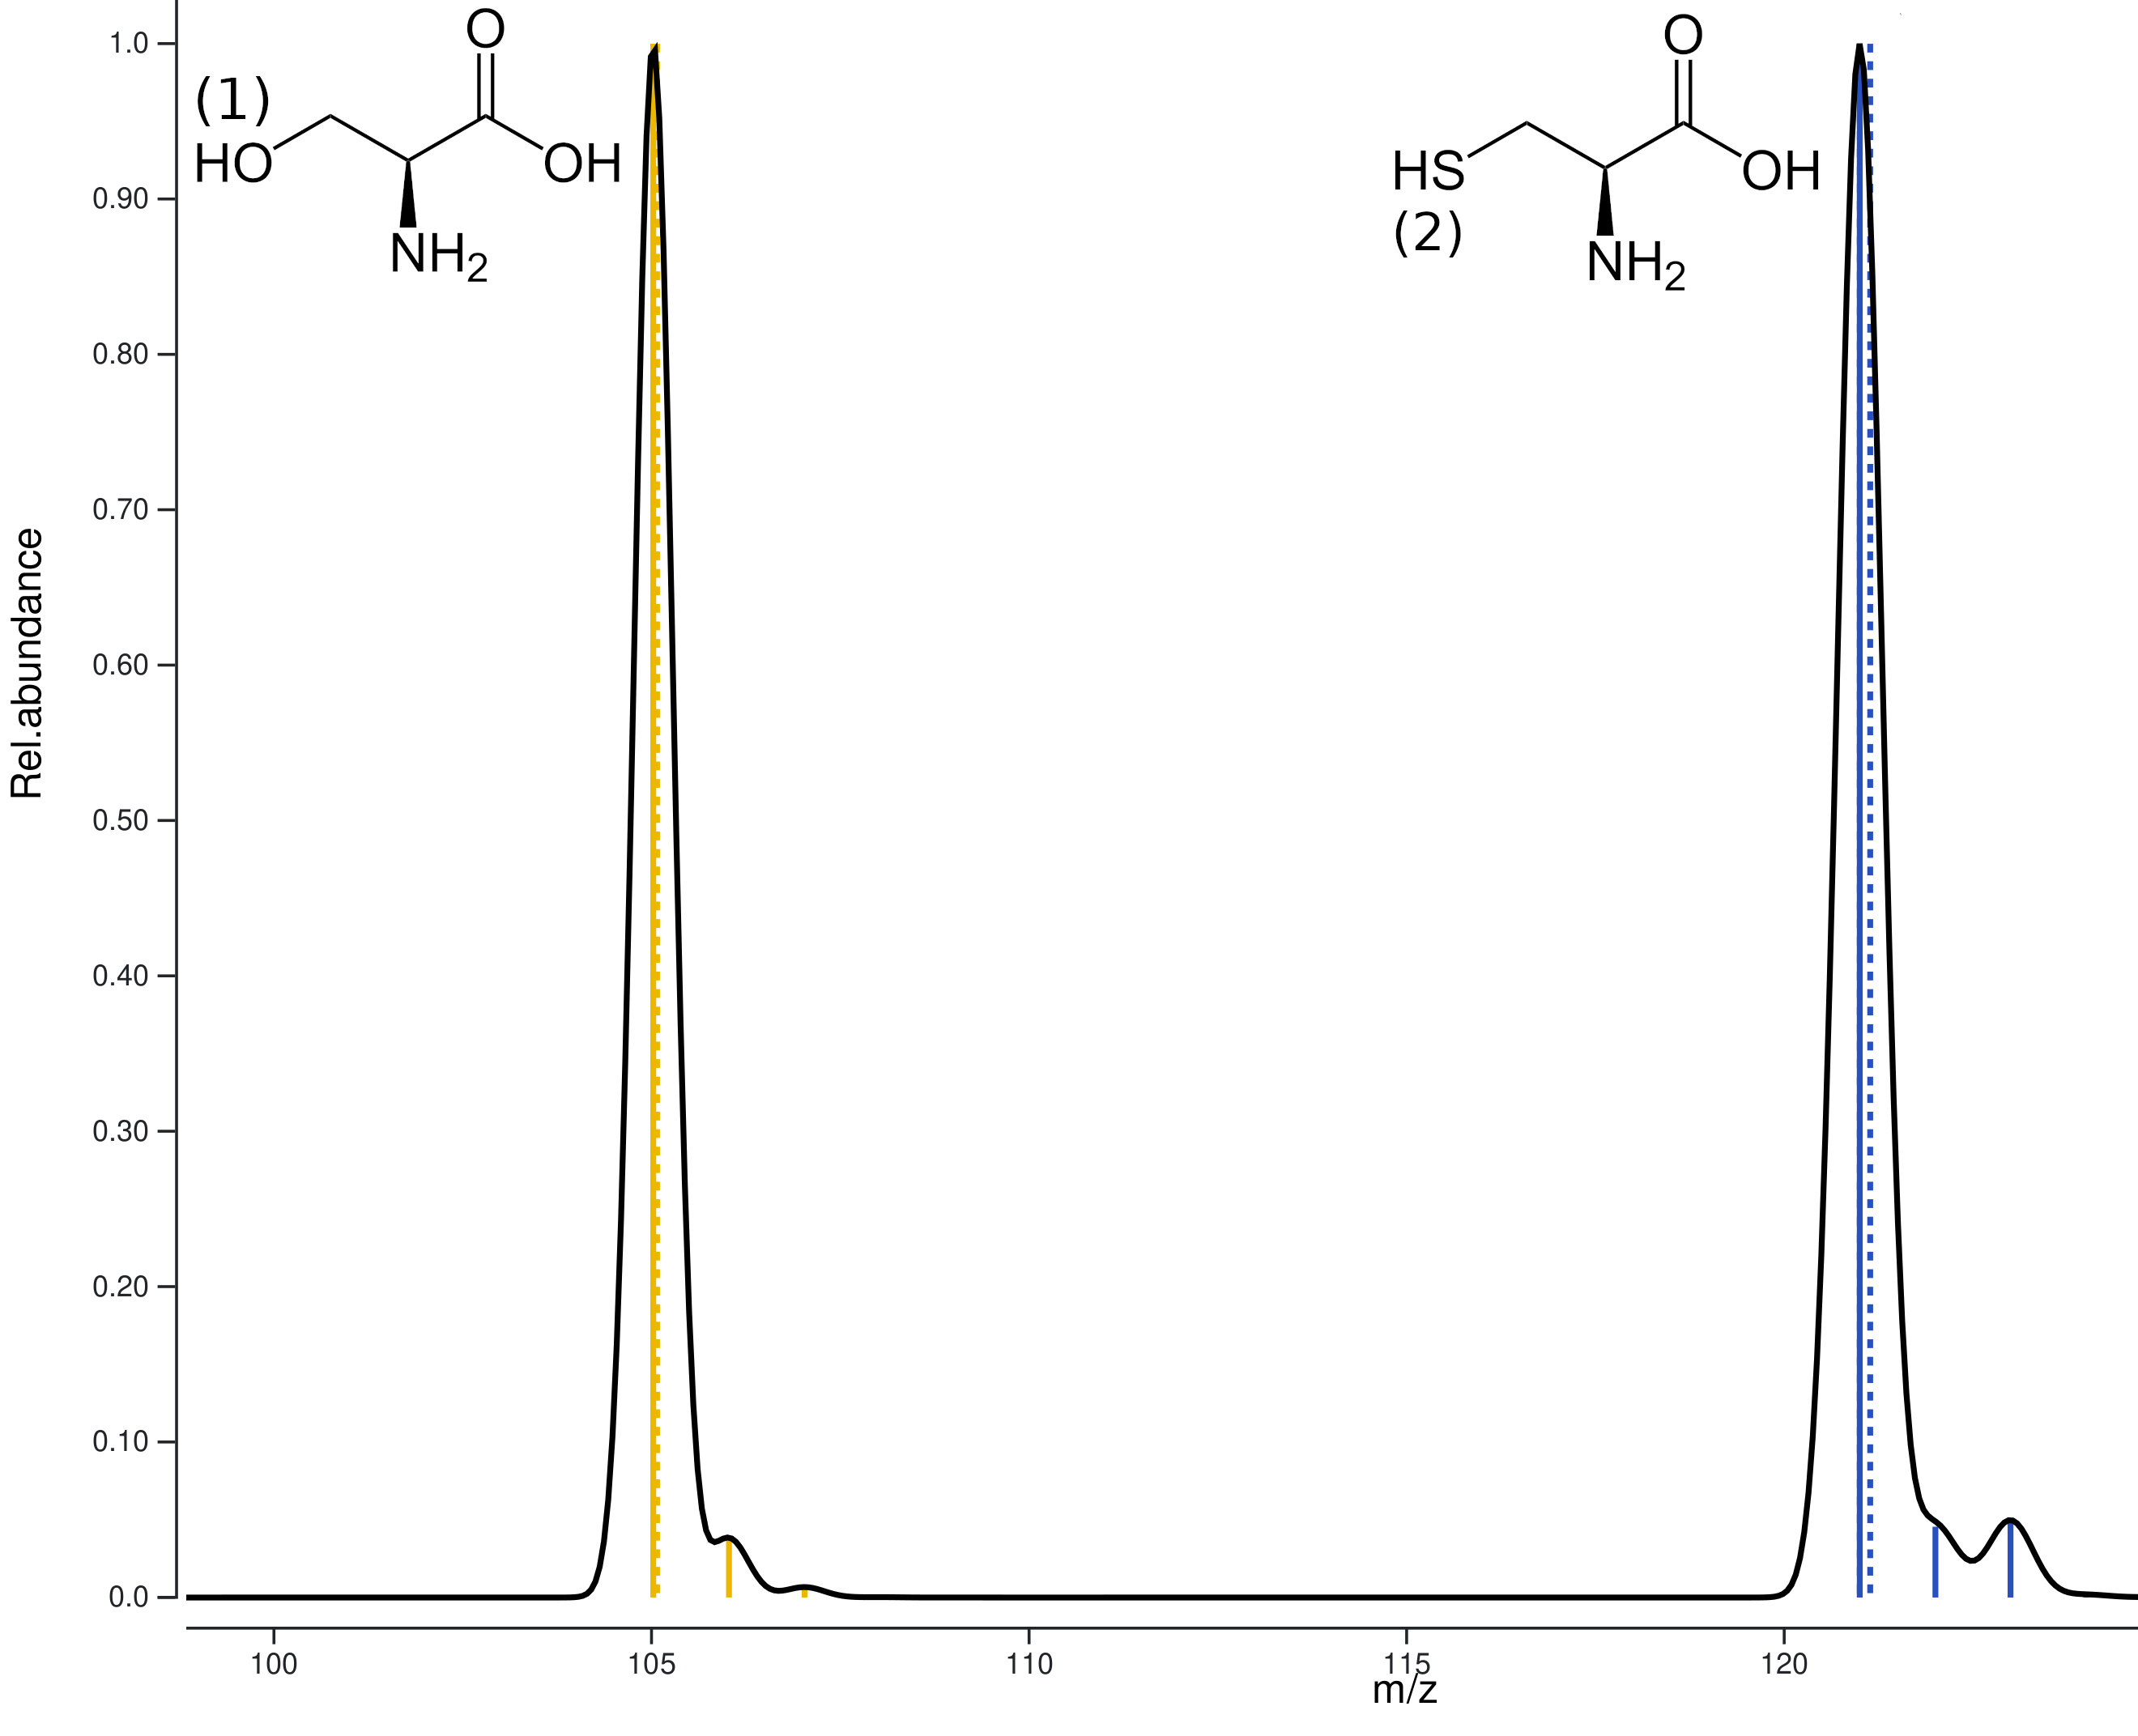
\includegraphics[width=0.75\textwidth]{./Resources/Simulated_Mass_Spectrum.png}
   \centering
   \caption{Computergeneriertes Massenspektrum von der Aminosäure \emph{Serin} (1) und \emph{Cystesin} (2). Peak von \emph{Serin} liegt bei 105; bei \emph{Systesin} um 121. y: relative Häufigkeit}
\end{figure}

Die Maxima werden \gerquot{Peaks} genannt und sind für eine Aminosäure an charakteristischer Position auf der $ x $-Achse. Obwohl sich die beiden Aminosäuren in der Abbildung \ref{fig:Sim_Mass_Spec} nur durch ein Atom unterscheiden (das linke Sauerstoffatom wurde durch ein Schwefelatom ersetzt) sind deren Massenspektren auf der $ x $-Achse weit voneinander entfernt und machen die beiden Aminosäuren dadurch sicher unterscheidbar.\\

Bei einzelnen Aminosäuren funktioniert die MS zuverlässig; bei Peptiden allerdings steht man vor dem Problem, dass das Massenspektrum unübersichtlicher wird und auch Peaks, die von Hintergrundrauschen stammen, schwerer herausgefiltert werden können. Abhilfe schafft hier die Tandem-Massenspektrometrie.

\subsection{Tandem-Massenspektrometrie (MS/MS)}\label{ss:Tandem_MS}
Bei der Tandem-Massenspektrometrie (MS/MS oder MS2) werden zwei MS Vorgänge hintereinander mit einer Probe durchgeführt. Die erste MS dient dazu Ionen aus einem bestimmten \massCharge Bereich auswählbar zu machen. Es entspricht also quasi einer Form der Filterung.

Vor der 2. MS werden die ausgewählten Reste einer Fragmentierung unterzogen. Bei einer Fragmentierung führt man Energie zu mit dem Ziel, dass die Ionen zerfallen und sog. Fragment-Ionen bilden. Diese Fragment-Ionen werden dann auf dem Massenspektrum nach der 2. MS sichtbar gemacht.

Fragment-Ionen sind kleiner als die ursprünglichen Ionen. So kann die 2. MS mit einer höheren Selektivität durchgeführt werden, welches Peaks durch Hintergrundrauschen verringert. Auch lassen sich Ionen besser identifizieren, die ein sehr ähnliches \massCharge-Verhältnis besitzen. Nach der 2. MS liegt eine Fülle an Fragment-Ionen-Peaks vor, aus denen sich die ursprünglichen Strukturinformationen ableiten lassen, da Ionen in spezifische Fragmente zerfallen \cite{Gross2013}. Zusammengefasst kann man sagen, dass das MS/MS Verfahren Ergebnisse höherer Güte erzeugt im Vergleich zur einfachen MS.

\section{De-Novo-Peptidsequenzierung mit \emph{pNovo+}}\label{s:pNovoPlusSeq}
Die \emph{pNovo+} Methode ist eine \gls{gls:DeNovo}, die mit einem \gls{gls:SpecGraph}en für die Auswertung der MS2-Spektren arbeitet und eine Erweiterung des \emph{pNovo} Verfahren darstellt \cite{pNovo}. Der Hauptansatz ist, dass zwei MS/MS Durchläufe mit jeweils verschiedenen Fragmentierungsmethoden\footnote{\emph{pNovo+} verwendet die higher energy
collisional dissociation (HCD) und die electron transfer dissociation (ETD) Fragmentierungsmethoden.} durchgeführt werden. Durch die Wahl einer anderen Fragmentierungsmethode ändert sich auch das MS2-Spektrum. Wenn nun Fragmentierungsmethoden verwendet werden, die möglichst komplementäre Spektren erzeugen, dann lässt sich durch das Zusammenführen der beiden MS2-Spektren die Qualität der Ergebnisse verbessern. Zum Beispiel lassen sich dadurch viele Peaks, die vom Hintergrundrauschen stammen, entfernen.

Für die Ermittlung der Sequenz eines Peptides wird zunächst ein Spektrums-Graph gebildet \dashAndSpace in Form eines DAG (directed acyclic graph). In diesem Graphen wird dann der längste Pfad bei gegebenen Start- und Endknoten berechnet. Die Reihenfolge der Knoten, die im längsten Pfad durchlaufen werden, stellt dann die Peptidsequenz dar.

\subsection{Vorverarbeitung der MS2-Spektren}\label{ss:Vorverarbeitung}
Bevor aus den MS2-Spektren der Spektrums-Graph gebildet werden kann, müssen die Daten vorverarbeitet werden. Für die Auswertung ist es von entscheidener Bedeutung, dass möglichst wenig Peaks verwendet werden, die vom Hintergrundrauschen stammen. Im weiteren Verlauf werden an einem exemplarischen MS2-Spektrum die Verarbeitungsschritte dargestellt.\\

Der erste Schritt ist das Verwenden des natürlichen Logarithmus der Intensitäten. Die Idee dabei ist, dass Hintergrundrauschen nicht überpriorisiert wird.

\begin{figure}[H]
   \centering
   \begin{minipage}[t]{.45\linewidth}
      \centering
      \begin{tikzpicture}[scale=\tikzScale, baseline=(current bounding box.center)]
         \draw [<->,thick] (0,\yAxisHeight) node (yaxis) [above] {\yAxisUnit}
         |- (\xAxisLength,0) node (xaxis) [right] {\xAxisUnit};
\draw[thick] (0.2, 0.0) -- (0.2, 2.3);
\draw[thick] (0.382, 0.0) -- (0.382, 1.7);
\draw[thick] (0.476, 0.0) -- (0.476, 2.7);
\draw[thick] (0.456, 0.0) -- (0.456, 1.8);
\draw[thick] (0.6859999999999999, 0.0) -- (0.6859999999999999, 2.7);
\draw[thick] (0.6839999999999999, 0.0) -- (0.6839999999999999, 1.8);
\draw[thick] (0.752, 0.0) -- (0.752, 1.1);
\draw[thick] (0.8200000000000001, 0.0) -- (0.8200000000000001, 2.2);
\draw[thick] (1.076, 0.0) -- (1.076, 1.5);
\draw[thick] (1.16, 0.0) -- (1.16, 1.9);
\draw[thick] (1.2120000000000002, 0.0) -- (1.2120000000000002, 2.0);
\draw[thick] (1.28, 0.0) -- (1.28, 1.9);
\draw[thick] (1.452, 0.0) -- (1.452, 1.3);
\draw[thick] (1.426, 0.0) -- (1.426, 1.9);
\draw[thick] (1.548, 0.0) -- (1.548, 1.9);
\draw[thick] (1.6740000000000002, 0.0) -- (1.6740000000000002, 1.5);
\draw[thick] (1.788, 0.0) -- (1.788, 2.5);
\draw[thick] (1.856, 0.0) -- (1.856, 2.3);
\draw[thick] (2.036, 0.0) -- (2.036, 1.7);
\draw[thick] (2.142, 0.0) -- (2.142, 1.6);
\draw[thick] (2.2520000000000002, 0.0) -- (2.2520000000000002, 2.0);
\draw[thick] (2.386, 0.0) -- (2.386, 1.6);
\draw[thick] (2.488, 0.0) -- (2.488, 2.9);
\draw[thick] (2.4739999999999998, 0.0) -- (2.4739999999999998, 2.7);
\draw[thick] (2.504, 0.0) -- (2.504, 2.0);
\draw[thick] (2.682, 0.0) -- (2.682, 2.0);
\draw[thick] (2.702, 0.0) -- (2.702, 2.5);
\draw[thick] (2.9259999999999997, 0.0) -- (2.9259999999999997, 2.8);
\draw[thick] (3.024, 0.0) -- (3.024, 2.4);
\draw[thick] (3.096, 0.0) -- (3.096, 1.8);
\draw[thick] (3.244, 0.0) -- (3.244, 2.6);
\draw[thick] (3.362, 0.0) -- (3.362, 1.9);
\draw[thick] (3.46, 0.0) -- (3.46, 2.3);
\draw[thick] (3.516, 0.0) -- (3.516, 1.1);
\draw[thick] (3.584, 0.0) -- (3.584, 1.8);
\draw[thick] (3.652, 0.0) -- (3.652, 2.0);
\draw[thick] (3.838, 0.0) -- (3.838, 1.5);
\draw[thick] (3.8819999999999997, 0.0) -- (3.8819999999999997, 2.6);
\draw[thick] (4.088, 0.0) -- (4.088, 2.6);
\draw[thick] (4.046, 0.0) -- (4.046, 1.1);
\draw[thick] (4.167999999999999, 0.0) -- (4.167999999999999, 2.0);
\draw[thick] (4.266, 0.0) -- (4.266, 2.4);
\draw[thick] (4.38, 0.0) -- (4.38, 1.1);
\draw[thick] (4.456, 0.0) -- (4.456, 2.2);
\draw[thick] (4.644, 0.0) -- (4.644, 2.6);
\draw[thick] (4.675999999999999, 0.0) -- (4.675999999999999, 2.5);
\draw[thick] (4.898000000000001, 0.0) -- (4.898000000000001, 1.2);
   \end{tikzpicture}%
   \end{minipage}%
   \textbf{$\rightarrow$} 
   \begin{minipage}[t]{.45\linewidth}
      \centering
      \begin{tikzpicture}[scale=\tikzScale, baseline=(current bounding box.center)]
      \draw [<->,thick] (0,\yAxisHeight) node (yaxis) [above] {\yAxisUnit}
      |- (\xAxisLength,0) node (xaxis) [right] {\xAxisUnit};
\draw[thick] (0.2, 0.0) -- (0.2, {ln(2.3)});
\draw[thick] (0.382, 0.0) -- (0.382, {ln(1.7)});
\draw[thick] (0.476, 0.0) -- (0.476, {ln(2.7)});
\draw[thick] (0.456, 0.0) -- (0.456, {ln(1.8)});
\draw[thick] (0.6859999999999999, 0.0) -- (0.6859999999999999, {ln(2.7)});
\draw[thick] (0.6839999999999999, 0.0) -- (0.6839999999999999, {ln(1.8)});
\draw[thick] (0.752, 0.0) -- (0.752, {ln(1.1)});
\draw[thick] (0.8200000000000001, 0.0) -- (0.8200000000000001, {ln(2.2)});
\draw[thick] (1.076, 0.0) -- (1.076, {ln(1.5)});
\draw[thick] (1.16, 0.0) -- (1.16, {ln(1.9)});
\draw[thick] (1.2120000000000002, 0.0) -- (1.2120000000000002, {ln(2.0)});
\draw[thick] (1.28, 0.0) -- (1.28, {ln(1.9)});
\draw[thick] (1.452, 0.0) -- (1.452, {ln(1.3)});
\draw[thick] (1.426, 0.0) -- (1.426, {ln(1.9)});
\draw[thick] (1.548, 0.0) -- (1.548, {ln(1.9)});
\draw[thick] (1.6740000000000002, 0.0) -- (1.6740000000000002, {ln(1.5)});
\draw[thick] (1.788, 0.0) -- (1.788, {ln(2.5)});
\draw[thick] (1.856, 0.0) -- (1.856, {ln(2.3)});
\draw[thick] (2.036, 0.0) -- (2.036, {ln(1.7)});
\draw[thick] (2.142, 0.0) -- (2.142, {ln(1.6)});
\draw[thick] (2.2520000000000002, 0.0) -- (2.2520000000000002, {ln(2.0)});
\draw[thick] (2.386, 0.0) -- (2.386, {ln(1.6)});
\draw[thick] (2.488, 0.0) -- (2.488, {ln(2.9)});
\draw[thick] (2.4739999999999998, 0.0) -- (2.4739999999999998, {ln(2.7)});
\draw[thick] (2.504, 0.0) -- (2.504, {ln(2.0)});
\draw[thick] (2.682, 0.0) -- (2.682, {ln(2.0)});
\draw[thick] (2.702, 0.0) -- (2.702, {ln(2.5)});
\draw[thick] (2.9259999999999997, 0.0) -- (2.9259999999999997, {ln(2.8)});
\draw[thick] (3.024, 0.0) -- (3.024, {ln(2.4)});
\draw[thick] (3.096, 0.0) -- (3.096, {ln(1.8)});
\draw[thick] (3.244, 0.0) -- (3.244, {ln(2.6)});
\draw[thick] (3.362, 0.0) -- (3.362, {ln(1.9)});
\draw[thick] (3.46, 0.0) -- (3.46, {ln(2.3)});
\draw[thick] (3.516, 0.0) -- (3.516, {ln(1.1)});
\draw[thick] (3.584, 0.0) -- (3.584, {ln(1.8)});
\draw[thick] (3.652, 0.0) -- (3.652, {ln(2.0)});
\draw[thick] (3.838, 0.0) -- (3.838, {ln(1.5)});
\draw[thick] (3.8819999999999997, 0.0) -- (3.8819999999999997, {ln(2.6)});
\draw[thick] (4.088, 0.0) -- (4.088, {ln(2.6)});
\draw[thick] (4.046, 0.0) -- (4.046, {ln(1.1)});
\draw[thick] (4.167999999999999, 0.0) -- (4.167999999999999, {ln(2.0)});
\draw[thick] (4.266, 0.0) -- (4.266, {ln(2.4)});
\draw[thick] (4.38, 0.0) -- (4.38, {ln(1.1)});
\draw[thick] (4.456, 0.0) -- (4.456, {ln(2.2)});
\draw[thick] (4.644, 0.0) -- (4.644, {ln(2.6)});
\draw[thick] (4.675999999999999, 0.0) -- (4.675999999999999, {ln(2.5)});
\draw[thick] (4.898000000000001, 0.0) -- (4.898000000000001, {ln(1.2)});
      \end{tikzpicture}
      \end{minipage}
      \caption{Anwendung des $ ln $ auf einem exemplarischen MS2-Spektrum.}
\end{figure}

Für das Verständnis des nächsten Schrittes muss man sich in Erinnerung rufen, dass eine gleiche Aminosäure keineswegs immer die gleiche Masse hat. Durch Isotope existiert eine gewisse \gerquot{Massenbandbreite} für ein und dieselbe Aminosäure. MS Systeme sind heute so genau, dass sie diese Differenzen erkennen. Dies hat den ungewollten Effekt, dass mehrere Peaks zu einer Aminosäure gehören können \cite{IsotopicDistributionMS}. Gleichzeitig können die \gerquot{Massenbandbreiten} zweier Aminosäuren sich überschneiden, sodass im ungünstigen Fall zwei Peaks kaum unterscheidbar nebeneinander liegen.\\

Eine Möglichkeit mit dieser Problematik umzugehen ist die Verwendung der monoisotopischen Masse. Die monoisotopische Masse ist die \gerquot{[...] exact mass of the most abundant naturally occurring stable isotope determined relative to the mass of 12 C, which is assigned the exact value of 12.0000.} \cite{MonoisotopicMass}. Ohne dabei jetzt tiefer ins Detail zu gehen kann man sagen, dass alle Peaks, deren Intensität mit einer möglichen monoisotopischen Masse übereinstimmen, auf jeden Fall einer Aminosäure entsprechen und (höchstwahrscheinlich)\footnote{Natürlich ist es möglich, dass das Rauschen zufällig einer monoisotopischen Masse entspricht. Die Wahrscheinlichkeit dafür ist allerdings sehr gering.} kein Hintergrundrauschen sind \cite{MassDefectMS}. Diese Peaks bekommen eine sogennante \emph{charge state}.\\

Der Algorithmus verwendet die \emph{charge state} Peaks als Ausganspunkte für weitere Berechnungen. Wenn die \massCharge Differenz zu einem anderen Peak einem Peptidfragment entspricht, dann stammt dieser Peak höchstwahrscheinlich von einem Fragment. Insgesamt werden damit die relevanten Peptidfragmente herausgeholt. Abbildung \ref{MonoisotopicMassFiltering} zeigt das Ergebnis nach den beiden zuvor genannten Schritten.

\begin{figure}[H]\label{MonoisotopicMassFiltering}
   \centering
   \begin{minipage}[t]{.45\linewidth}
      \centering
      \begin{tikzpicture}[scale=\tikzScale, baseline=(current bounding box.center)]
         \draw [<->,thick] (0,\yAxisHeight) node (yaxis) [above] {\yAxisUnit}
         |- (\xAxisLength,0) node (xaxis) [right] {\xAxisUnit};
\draw[thick] (0.2, 0.0) -- (0.2, {ln(2.3)});
\draw[color=blue!85!,opacity=.55,thick] (0.382, 0.0) -- (0.382, {ln(1.7)});
\draw[color=blue!85!,opacity=.55,thick] (0.476, 0.0) -- (0.476, {ln(2.7)});
\draw[color=magenta,thick] (0.456, 0.0) -- (0.456, {ln(1.8)});
\draw[color=blue!85!,opacity=.55,thick] (0.6859999999999999, 0.0) -- (0.6859999999999999, {ln(2.7)});
\draw[color=blue!85!,opacity=.55,thick] (0.6839999999999999, 0.0) -- (0.6839999999999999, {ln(1.8)});
\draw[thick] (0.752, 0.0) -- (0.752, {ln(1.1)});
\draw[thick] (0.8200000000000001, 0.0) -- (0.8200000000000001, {ln(2.2)});
\draw[thick] (1.076, 0.0) -- (1.076, {ln(1.5)});
\draw[thick] (1.16, 0.0) -- (1.16, {ln(1.9)});
\draw[thick] (1.2120000000000002, 0.0) -- (1.2120000000000002, {ln(2.0)});
\draw[thick] (1.28, 0.0) -- (1.28, {ln(1.9)});
\draw[color=blue!85!,opacity=.55,thick] (1.452, 0.0) -- (1.452, {ln(1.3)});
\draw[color=blue!85!,opacity=.55,thick] (1.426, 0.0) -- (1.426, {ln(1.9)});
\draw[color=magenta,thick] (1.548, 0.0) -- (1.548, {ln(1.9)});
\draw[color=blue!85!,opacity=.55,thick] (1.6740000000000002, 0.0) -- (1.6740000000000002, {ln(1.5)});
\draw[color=blue!85!,opacity=.55,thick] (1.788, 0.0) -- (1.788, {ln(2.5)});
\draw[thick] (1.856, 0.0) -- (1.856, {ln(2.3)});
\draw[thick] (2.036, 0.0) -- (2.036, {ln(1.7)});
\draw[thick] (2.142, 0.0) -- (2.142, {ln(1.6)});
\draw[thick] (2.2520000000000002, 0.0) -- (2.2520000000000002, {ln(2.0)});
\draw[thick] (2.386, 0.0) -- (2.386, {ln(1.6)});
\draw[color=blue!85!,opacity=.55,thick] (2.488, 0.0) -- (2.488, {ln(2.9)});
\draw[thick] (2.4739999999999998, 0.0) -- (2.4739999999999998, {ln(2.7)});
\draw[color=blue!85!,opacity=.55,thick] (2.504, 0.0) -- (2.504, {ln(2.0)});
\draw[color=magenta,thick] (2.682, 0.0) -- (2.682, {ln(2.0)});
\draw[color=blue!85!,opacity=.55,thick] (2.702, 0.0) -- (2.702, {ln(2.5)});
\draw[thick] (2.9259999999999997, 0.0) -- (2.9259999999999997, {ln(2.8)});
\draw[thick] (3.024, 0.0) -- (3.024, {ln(2.4)});
\draw[thick] (3.096, 0.0) -- (3.096, {ln(1.8)});
\draw[thick] (3.244, 0.0) -- (3.244, {ln(2.6)});
\draw[thick] (3.362, 0.0) -- (3.362, {ln(1.9)});
\draw[color=blue!85!,opacity=.55,thick] (3.46, 0.0) -- (3.46, {ln(2.3)});
\draw[color=blue!85!,opacity=.55,thick] (3.516, 0.0) -- (3.516, {ln(1.1)});
\draw[color=blue!85!,opacity=.55,thick] (3.584, 0.0) -- (3.584, {ln(1.8)});
\draw[color=magenta,thick] (3.652, 0.0) -- (3.652, {ln(2.0)});
\draw[color=blue!85!,opacity=.55,thick] (3.838, 0.0) -- (3.838, {ln(1.5)});
\draw[color=blue!85!,opacity=.55,thick] (3.8819999999999997, 0.0) -- (3.8819999999999997, {ln(2.6)});
\draw[thick] (4.088, 0.0) -- (4.088, {ln(2.6)});
\draw[thick] (4.046, 0.0) -- (4.046, {ln(1.1)});
\draw[thick] (4.167999999999999, 0.0) -- (4.167999999999999, {ln(2.0)});
\draw[thick] (4.266, 0.0) -- (4.266, {ln(2.4)});
\draw[color=blue!85!,opacity=.55,thick] (4.38, 0.0) -- (4.38, {ln(1.1)});
\draw[color=blue!85!,opacity=.55,thick] (4.456, 0.0) -- (4.456, {ln(2.2)});
\draw[color=magenta,thick] (4.644, 0.0) -- (4.644, {ln(2.6)});
\draw[color=blue!85!,opacity=.55,thick] (4.675999999999999, 0.0) -- (4.675999999999999, {ln(2.5)});
\draw[color=blue!85!,opacity=.55,thick] (4.898000000000001, 0.0) -- (4.898000000000001, {ln(1.2)});
   \end{tikzpicture}%
   \end{minipage}%
   \textbf{$\rightarrow$} 
   \begin{minipage}[t]{.45\linewidth}
      \centering
      \begin{tikzpicture}[scale=\tikzScale, baseline=(current bounding box.center)]
      \draw [<->,thick] (0,\yAxisHeight) node (yaxis) [above] {\yAxisUnit}
      |- (\xAxisLength,0) node (xaxis) [right] {\xAxisUnit};
\draw[color=blue!85!,opacity=.55,thick] (0.382, 0.0) -- (0.382, {ln(1.7)});
\draw[color=blue!85!,opacity=.55,thick] (0.476, 0.0) -- (0.476, {ln(2.7)});
\draw[color=magenta,thick] (0.456, 0.0) -- (0.456, {ln(1.8)});
\draw[color=blue!85!,opacity=.55,thick] (0.6859999999999999, 0.0) -- (0.6859999999999999, {ln(2.7)});
\draw[color=blue!85!,opacity=.55,thick] (0.6839999999999999, 0.0) -- (0.6839999999999999, {ln(1.8)});
\draw[color=blue!85!,opacity=.55,thick] (1.452, 0.0) -- (1.452, {ln(1.3)});
\draw[color=blue!85!,opacity=.55,thick] (1.426, 0.0) -- (1.426, {ln(1.9)});
\draw[color=magenta,thick] (1.548, 0.0) -- (1.548, {ln(1.9)});
\draw[color=blue!85!,opacity=.55,thick] (1.6740000000000002, 0.0) -- (1.6740000000000002, {ln(1.5)});
\draw[color=blue!85!,opacity=.55,thick] (1.788, 0.0) -- (1.788, {ln(2.5)});
\draw[color=blue!85!,opacity=.55,thick] (2.488, 0.0) -- (2.488, {ln(2.9)});
\draw[color=blue!85!,opacity=.55,thick] (2.504, 0.0) -- (2.504, {ln(2.0)});
\draw[color=magenta,thick] (2.682, 0.0) -- (2.682, {ln(2.0)});
\draw[color=blue!85!,opacity=.55,thick] (2.702, 0.0) -- (2.702, {ln(2.5)});
\draw[color=blue!85!,opacity=.55,thick] (3.46, 0.0) -- (3.46, {ln(2.3)});
\draw[color=blue!85!,opacity=.55,thick] (3.516, 0.0) -- (3.516, {ln(1.1)});
\draw[color=blue!85!,opacity=.55,thick] (3.584, 0.0) -- (3.584, {ln(1.8)});
\draw[color=magenta,thick] (3.652, 0.0) -- (3.652, {ln(2.0)});
\draw[color=blue!85!,opacity=.55,thick] (3.838, 0.0) -- (3.838, {ln(1.5)});
\draw[color=blue!85!,opacity=.55,thick] (3.8819999999999997, 0.0) -- (3.8819999999999997, {ln(2.6)});
\draw[color=blue!85!,opacity=.55,thick] (4.38, 0.0) -- (4.38, {ln(1.1)});
\draw[color=blue!85!,opacity=.55,thick] (4.456, 0.0) -- (4.456, {ln(2.2)});
\draw[color=magenta,thick] (4.644, 0.0) -- (4.644, {ln(2.6)});
\draw[color=blue!85!,opacity=.55,thick] (4.675999999999999, 0.0) -- (4.675999999999999, {ln(2.5)});
\draw[color=blue!85!,opacity=.55,thick] (4.898000000000001, 0.0) -- (4.898000000000001, {ln(1.2)});
      \end{tikzpicture}
      \end{minipage}
      \caption{Entfernen von Peaks, die keiner monoisotopischen Masse entsprechen oder benachbart mit einer Differenz von einem Fragment-Ion sind.}
\end{figure}

Tatsächlich ist die Verarbeitung an dieser Stelle noch etwas komplexer. So existieren auch noch sogenannte \emph{isotopic cluster}\footnote{Definition eines \emph{isotopic cluster} nach IUPAC: \gerquot{Group of peaks representing ions of the same elemental composition, but different isotopic compositions.} \cite[1556]{IUPACDefinitions}}, die gesondert verarbeitet werden. Für das grundsätzliche Prinzip ist dieses Detail allerdings weniger relevant.\\

Im letzten Vorberarbeitungsschritt werden Peaks aus einem irrelevanten \massCharge Bereich entfernt und naheliegende Peaks werden zusammengefasst, indem der Mittelwert sowol des \massCharge Wertes als auch der der Intensität besimmt wird. Üblicherweise liegt der Bereich für das Zusammenfassen bei $ +- 20 ppm $.

\begin{figure}[H]
   \centering
   \begin{minipage}[t]{.45\linewidth}
      \centering
      \begin{tikzpicture}[scale=\tikzScale, baseline=(current bounding box.center)]
         \draw [<->,thick] (0,\yAxisHeight) node (yaxis) [above] {\yAxisUnit}
         |- (\xAxisLength,0) node (xaxis) [right] {\xAxisUnit};
\draw[thick] (0.382, 0.0) -- (0.382, {ln(1.7)});
\draw[thick] (0.476, 0.0) -- (0.476, {ln(2.7)});
\draw[thick] (0.456, 0.0) -- (0.456, {ln(1.8)});
\draw[thick] (0.6859999999999999, 0.0) -- (0.6859999999999999, {ln(2.7)});
\draw[thick] (0.6839999999999999, 0.0) -- (0.6839999999999999, {ln(1.8)});
\draw[color=red,thick] (1.452, 0.0) -- (1.452, {ln(1.3)});
\draw[color=red,thick] (1.426, 0.0) -- (1.426, {ln(1.9)});
\draw[thick] (1.548, 0.0) -- (1.548, {ln(1.9)});
\draw[thick] (1.6740000000000002, 0.0) -- (1.6740000000000002, {ln(1.5)});
\draw[thick] (1.788, 0.0) -- (1.788, {ln(2.5)});
\draw[color=red,thick] (2.488, 0.0) -- (2.488, {ln(2.9)});
\draw[color=red,thick] (2.504, 0.0) -- (2.504, {ln(2.0)});
\draw[color=red,thick] (2.682, 0.0) -- (2.682, {ln(2.0)});
\draw[color=red,thick] (2.702, 0.0) -- (2.702, {ln(2.5)});
\draw[thick] (3.46, 0.0) -- (3.46, {ln(2.3)});
\draw[thick] (3.516, 0.0) -- (3.516, {ln(1.1)});
\draw[thick] (3.584, 0.0) -- (3.584, {ln(1.8)});
\draw[thick] (3.652, 0.0) -- (3.652, {ln(2.0)});
\draw[color=red,thick] (3.838, 0.0) -- (3.838, {ln(1.5)});
\draw[color=red,thick] (3.8819999999999997, 0.0) -- (3.8819999999999997, {ln(2.6)});
\draw[thick] (4.38, 0.0) -- (4.38, {ln(1.1)});
\draw[thick] (4.456, 0.0) -- (4.456, {ln(2.2)});
\draw[thick] (4.644, 0.0) -- (4.644, {ln(2.6)});
\draw[thick] (4.675999999999999, 0.0) -- (4.675999999999999, {ln(2.5)});
\draw[thick] (4.898000000000001, 0.0) -- (4.898000000000001, {ln(1.2)});

\fill[red!25!,opacity=.25] (0,0) rectangle (1,\yAxisHeight-\axisColorOffset);
         \fill[red!25!,opacity=.25] (\xAxisLength-1,0) rectangle (\xAxisLength-\axisColorOffset,\yAxisHeight-\axisColorOffset);
         \fill[green!25!,opacity=.25] (1,0) rectangle (\xAxisLength-1,\yAxisHeight-\axisColorOffset);
   \end{tikzpicture}%
   \end{minipage}%
   \textbf{$\rightarrow$} 
   \begin{minipage}[t]{.45\linewidth}
      \centering
      \begin{tikzpicture}[scale=\tikzScale, baseline=(current bounding box.center)]
      \draw [<->,thick] (0,\yAxisHeight) node (yaxis) [above] {\yAxisUnit}
      |- (\xAxisLength,0) node (xaxis) [right] {\xAxisUnit};
%\draw[color=red,thick] (1.452, 0.0) -- (1.452, {ln(1.3)});
%\draw[color=red,thick] (1.426, 0.0) -- (1.426, {ln(1.9)});
\draw[color=red,ultra thick] ({(1.452+1.426)/2}, 0.0) -- ({(1.452+1.426)/2}, {(ln(1.3)+ln(1.9))/2});

\draw[thick] (1.548, 0.0) -- (1.548, {ln(1.9)});
\draw[thick] (1.6740000000000002, 0.0) -- (1.6740000000000002, {ln(1.5)});
\draw[thick] (1.788, 0.0) -- (1.788, {ln(2.5)});

%\draw[color=red,thick] (2.488, 0.0) -- (2.488, {ln(2.9)});
%\draw[color=red,thick] (2.504, 0.0) -- (2.504, {ln(2.0)});
\draw[color=red,ultra thick] ({(2.488+2.504)/2}, 0.0) -- ({(2.488+2.504)/2}, {(ln(2.9)+ln(2.0))/2});

%\draw[color=red,thick] (2.682, 0.0) -- (2.682, {ln(2.0)});
%\draw[color=red,thick] (2.702, 0.0) -- (2.702, {ln(2.5)});
\draw[color=red,ultra thick] ({(2.682+2.702)/2}, 0.0) -- ({(2.682+2.702)/2}, {(ln(2.0+ln(2.5))/2});

\draw[thick] (3.46, 0.0) -- (3.46, {ln(2.3)});
\draw[thick] (3.516, 0.0) -- (3.516, {ln(1.1)});
\draw[thick] (3.584, 0.0) -- (3.584, {ln(1.8)});
\draw[thick] (3.652, 0.0) -- (3.652, {ln(2.0)});

%\draw[color=red,thick] (3.838, 0.0) -- (3.838, {ln(1.5)});
%\draw[color=red,thick] (3.8819999999999997, 0.0) -- (3.8819999999999997,{ln(2.6)});
\draw[color=red,ultra thick] ({(3.838+3.8819999999999997)/2}, 0.0) -- ({(3.838+3.8819999999999997)/2}, {(ln(1.5)+ln(2.6))/2});

\fill[red!25!,opacity=.25] (0,0) rectangle (1,\yAxisHeight-\axisColorOffset);
         \fill[red!25!,opacity=.25] (\xAxisLength-1,0) rectangle (\xAxisLength-\axisColorOffset,\yAxisHeight-\axisColorOffset);
         \fill[green!25!,opacity=.25] (1,0) rectangle (\xAxisLength-1,\yAxisHeight-\axisColorOffset);
      \end{tikzpicture}
      \end{minipage}
      \caption{Entfernen von Peaks aus einem irrelevanten \massCharge Bereich und zusammenfassen naheliegender Peaks. Rot markierte Peaks sind jene, die zusammengefasst werden.}
\end{figure}

\subsection{Bildung eines Spektrums-Graphen}\label{ss:BildungSpekGraph}
Der Spektrums-Graph wird aus einem vorverarbeiteten MS2-Spektrum (siehe Kapitel: \ref{ss:Vorverarbeitung}) gebildet. Im initialen Zustand werden die Peaks als Knoten interpretiert. Dazu kommt ein Start- und Endknoten. Jedem Knoten wird eine Masse zugeordet; im initialen Zustand bekommt der Startknoten die Masse 0 und der Endknoten die Masse des vorherigen Knotens minus der Masse des Wassers ($ 18,02 $). Die Masse der übrigen Knoten entsprechen ihren jeweils korrespondierenden \massCharge Wert. Die gerichteten Kanten werden zwischen einem Knotenpaar hinzugefügt, wenn die Differenz deren Masse gleich ist mit der Masse von ein oder zwei Aminosäuren.

\subsection{Identifikation der Aminosäuresequenz}
Der gebildete DAG kann mit klassischen Algorithmen, die den längsten Pfad suchen, durchlaufen werden. Bezogen auf die Graphentheorie entspricht die Ermittlung der Aminosäurensequenz dem Suchen eines bestimmten Pfades \dashAndSpace und nicht nach irgendeinem Pfad. Daher muss der Algorithmus mittels einer Breitensuche arbeiten, um alle möglichen Pfade zu bestimmen.

In aller Regel wird es mehrere Pfade geben. Bestimmte Sequenzen sind wahrscheinlicher als andere. So sind Pfade mit Kanten, die wegen der Massendifferenz von genau einer Aminosäure gebildet wurden, wahrscheinlicher \cite{pNovoPlus}. Alle Pfade bekommen mittels einer Scoring-Funktion einen Wert zugewiesen. Der Pfad mit dem höchsten Scoring-Wert ist wahrscheinlich das richtige Ergebnis. Die Scoring-Funktion berücksichtigt unter anderem wie viele Fragmente, die einer bestimmten Aminosäure zugeordet werden können, im MS2-Spektrum vorhanden sind \cite{pNovo}. Die Sequenz mit dem höchsten Scoring-Wert ist das Endergebnis.

\section{De-Novo-Peptidsequenzierung mit \emph{Open-pNovo}}\label{s:OpenpNovoSeq}
Bei Proteinen können posttranslationale Proteinmodifikationen (PTM) auftreten. PTMs sind Ereignisse, bei denen sich Änderungen im Protein einstellen \cite{Mann2003}; teilweise sind die Änderungen von einer Zelle erwünscht \dashAndSpace teilweise stammen sie aber auch zum Beispiel von unerwünschten Wechselwirkungen nebeneinanderliegenden Aminosäuren. Ein Teil dieser PTMs führen zu einer Änderung der Aminosäuresequenz. Dies ist für die \gls{gls:DeNovo} nicht weiter problematisch, da sowieso ohne eine Datenbank gearbeitet wird, sodass solche PTMs nicht einmal auffallen würden. Andere PTMs hingegen haben die Auswirkung, dass Stoffe gebildet werden, die nicht mehr zu der Gruppe der proteinogenen Aminosäuren gehören. Proteinogene Aminosäuren sind jene Aminosäuren, die für den Bau von Proteinen verwendet werden. Der Effekt ist also, dass Stoffe (oder deren Fragmente) bei einem Massenspektrum angezeigt werden, die kein Teil eines Peptids sein können. Bei der Sequenzierung von Peptidfragmenten muss dies daher berücksichtigt werden.
Wenn im weiteren Verlauf von PTMs gesprochen wird, dann sind solche gemeint, die für die \gls{gls:DeNovo} relevant sind.

Open-pNovo ist ein \gls{gls:DeNovo}sverfahren, welches auf pNovo+ Tool aufbaut und versucht die Problematik mit den PTMs zu lösen.

\subsection{PTMs im konstruierten DAG}
Die Konvertierung eines MS2-Spektrums läuft bis zum DAG analog ab wie in den Kapiteln \ref{ss:Vorverarbeitung} und \ref{ss:BildungSpekGraph} für pNovo+. Der Unterschied ist nun, dass es zwei Arten von Kanten gibt:

\begin{itemize}
   \item \gerquot{Normale} Kanten: Kanten, die gebildet werden, wie es bereits für \emph{pNovo+} gezeigt wurde. 
   \item \gerquot{Modifizierte} Kanten: Kanten, die zum Grahpen hinzugefügt werden, wenn die Massendifferenz zweier Knoten der Masse einer Aminosäure plus der Masse einer möglichen PTM-Änderung entspricht. 
\end{itemize}

Eine Liste aller PTMs in der Datenbank Unimod (sowohl relevante als auch nicht relevante) beinhaltet aktuell 1510 Einträge\footnote{Siehe: \url{https://www.ebi.ac.uk/ols/ontologies/unimod}} (Stand: 18.04.2022). Für die modifizierten Kanten gibt es insgesamt $ 1510 * 20 = 30200 $ mögliche Differenzen, wobei viele davon nicht relevante PTMs sind. Zum Vergleich: bei den normalen Kanten gibt es $ 20^2 = 400 $ mögliche Differenzen.

Die hohe Anzahl an Differenzen für modifizierte Kanten hat die Konsequenz, dass viele Knoten zufällig verbunden werden und dass dadurch die Genauigkeit der Ergebnisse abnimmt. Dieses Problem kann man durch eine geringere Liste an möglichen PTMs abfedern, allerdings mit einem Verlust  der Genauigkeit auf Seiten der PTMs. Es ist hier also eine Abwägung.

\subsection{Evaluierung von Open-pNovo}
Open-pNovo wurde sowohl auf drei realen als auch auf drei generierten Testdaten getestet. Tabelle \ref{tab:OpenPNovoResults} zeigt die Ergebnisse im Vergleich zu pNovo+ und zwei anderen Algorithmen. Die Datensätze enthielten die am häufigsten vorkommenden PTMs.

\begin{table}[H]
    \centering
    \begin{tabular}{l|c|c|c|c}
        \toprule
        \textbf{Testdatensätze} & \textbf{Open-pNovo+} & \textbf{pNovo+} & \textbf{PEAKS} & \textbf{Novor} \\
        \midrule
        Real (20259) & $76,3 \%$ & $68,5 \%$ & $65,8 \%$ & $39,9 \%$ \\
        Generiert (17877) & $77,8 \%$ & $0,6 \%$ & $0,5 \%$ & $0,2 \%$ \\
        \bottomrule
    \end{tabular}
    \newline
    \caption{Vergleich der durchschnittlichen richtigen \gls{gls:DeNovo} Peptidsequenzierungen von Open-pNovo und anderen Algorithmen \cite[650]{OpenPNovo}.}
    \label{tab:OpenPNovoResults}
\end{table}

Die enorm schlechten Ergebnisse der anderen Algorithmen bei den generierten Testdaten ist ein Nebeneffekt des Ziels bei der Testdatengenerierung. Denn diese wurden so ausgelegt, um die Grenzen von Open-pNovo+ zu ermitteln \cite[649]{OpenPNovo}. Eine Aussagekraft haben diese Ergebnisse also nicht. Allerdings auch bei realen Testdaten zeigt sich Open-pNovo als voll konkurrenzfähig gegenüber den anderen Algorithmen.

Noch besser zeigt sich Open-pNovo, wenn der Recall Wert betrachtet wird \dashAndSpace also die Anzahl an verschiedenen PSMs, die erkannt wurden. In diesem Fall ist der Abstand zu den anderen Algorithmen deutlich größer geworden.

\begin{table}[H]
    \centering
    \begin{tabular}{l|c|c|c|c}
        \toprule
        \textbf{Testdatensätze} & \textbf{Open-pNovo+} & \textbf{pNovo+} & \textbf{PEAKS} & \textbf{Novor} \\
        \midrule
        Real (5034) & $61,6 \%$ & $31,3 \%$ & $32,0 \%$ & $13,7 \%$ \\
        \bottomrule
    \end{tabular}
    \newline
    \caption{Vergleich der durchschnittlichen Recall Werte einer \gls{gls:DeNovo} Peptidsequenzierungen von Open-pNovo und anderen Algorithmen \cite[650]{OpenPNovo}.}
    \label{tab:OpenPNovoResultsRecall}
\end{table}

\subsection{Zusammenfassung}


% Die \gls{gls:DeNovo} nutzt die sogenannte \gls{gls:TMassSpek} für die Bestimmung der Peptidsequenz. Dabei wird die physikalische Eigenschaft ausgenutzt, dass jedes Atom bzw. jedes Molekül \dashAndSpace wenn es einer \gls{gls:Ionisation} unterzogen wurde \dashAndSpace ein charakteristisches \gls{gls:MassSpek} besitzt. Das \gls{gls:MassSpek} stellt also eine Art \gerquot{Fingerabdruck} eines Moleküls dar und macht dieses ermittelbar.

% U.U. eine Beispielgrafik eines Massenspektrums hinzufuegen ...

\subsubsection{\glsentrytext{gls:TMassSpek} bei größeren Molekülen}
Bei größeren Molekülen (wie einem Protein) führt die \gls{gls:Ionisation} dazu, dass das Molekül in kleinere spezifische Ionen zerfällt (sog. Fragmentierung). Die Fragmentierungsinformationen einer \gls{gls:DeNovo} sind meist unvollständig, da fehlende Daten bei einem Fragmentierungsschritt die Güte des Endergebnisses negativ beeinflusst. Dies wird insbesondere dann ein Problem, wenn unbekannte Änderungen in einer Peptidsequenz vorhanden sind.

Um dieses Problem zu verringern können unterschiedliche Techniken parallel eingesetzt werden, welche verschiedene Fragmente erzeugen und daher auch verschiedenartige \glspl{gls:MassSpek} zur Folge haben.\footnote{Konkret: Es wird sowohl das \gls{acr:HCD} als auch das \gls{acr:ETD} Verfahren angewendet.}

\subsection{Datenaufbereitung}
Typischerweise betrachtet man die sog. \gerquot{\glspl{gls:Peak}} in den \glspl{gls:MassSpek}. Jeder \gls{gls:Peak} stellt ein unterschiedliches Ion dar. Dazu kommen Messungenauigkeiten sowie Hintergrundrauschen. Durch die hohe Anzahl an möglichen Ionen kann nicht ohne weiteres differenziert werden, welcher der \glspl{gls:Peak} von welchen Ionen erzeugt wurden und welche nicht.

% Frage an Dominik: Ist hier eine einfache Auflistung an Techniken für die Datenaufbereitung besser?
Der Algorithmus für die Datenaufbereitung berechnet den natürlichen Logarithmus von den Intensitäten der \glspl{gls:Peak}, um Hintergrundrauschen und Messungenauigkeiten nicht überzupriorisieren. Zusätzlich dazu werden \glspl{gls:Peak}, die in einem Toleranzbereich nebeneinander liegen, zusammengefasst. Am Ende werden die \glspl{gls:Peak} entfernt, bei denen bekannt ist, dass es sich nicht um relevante Ionen handeln kann. (z.B. \glspl{gls:Peak} von Isotopen)

\begin{figure}[H]
   \centering
   \begin{minipage}[t]{.4\linewidth}
      \centering
      \begin{tikzpicture}[scale=\tikzScale, baseline=(current bounding box.center)]
         \draw [<->,thick] (0,2.75) node (yaxis) [above] {\yAxisUnit}
         |- (3,0) node (xaxis) [right] {\xAxisUnit};

         \draw[thick] (0.2,0) -- (0.2,1.1);
         \draw[thick] (0.3,0) -- (0.3,1.6);
         \draw[thick] (0.6,0) -- (0.6,1.7);
         \draw[thick] (0.8,0) -- (0.8,1.2);
         \draw[thick] (1.0,0) -- (1.0,1.1);

         \draw[color=red,thick] (1.2,0) -- (1.2,2.65);
         \draw[thick] (1.4,0) -- (1.4,1.4);
         \draw[thick] (1.6,0) -- (1.6,1.2);
         \draw[thick] (1.8,0) -- (1.8,1.3);
         \draw[thick] (2.0,0) -- (2.0,1.8);

         \draw[thick] (1.1,0) -- (1.1,2.0);
         \draw[color=red,thick] (0.35,0) -- (0.35,2.25);
         \draw[thick] (1.9,0) -- (1.9,1.4);
         \draw[color=red,thick] (2.2,0) -- (2.2,2.6);
         \draw[thick] (2.5,0) -- (2.5,1.25);

         \draw[thick] (2.7,0) -- (2.7,1.1);
         \foreach \x in {1,...,6}
         {
            \draw[thick] (1.2+\x*0.05,0) -- (1.2+\x*0.05,1.0+\x*0.15);
         }
      \end{tikzpicture}%
      % \subcaption{Exemplarische Rohdaten}
   \end{minipage}%
   \textbf{$\rightarrow$}
   \begin{minipage}[t]{.4\linewidth}
      \centering
      \begin{tikzpicture}[scale=\tikzScale, baseline=(current bounding box.center)]
         \draw [<->,thick] (0,2.75) node (yaxis) [above] {\yAxisUnit}
         |- (3,0) node (xaxis) [right] {\xAxisUnit};

         \draw[thick] (0.2,0) -- (0.2,{ln(1.1)});
         \draw[thick] (0.3,0) -- (0.3,{ln(1.6)});
         \draw[thick] (0.6,0) -- (0.6,{ln(1.7)});
         \draw[thick] (0.8,0) -- (0.8,{ln(1.2)});
         \draw[thick] (1.0,0) -- (1.0,{ln(1.1)});

         \draw[color=red,thick] (1.2,0) -- (1.2,{ln(2.65)});
         \draw[thick] (1.4,0) -- (1.4,{ln(1.4)});
         \draw[thick] (1.6,0) -- (1.6,{ln(1.2)});
         \draw[thick] (1.8,0) -- (1.8,{ln(1.3)});
         \draw[thick] (2.0,0) -- (2.0,{ln(1.8)});

         \draw[thick] (1.1,0) -- (1.1,{ln(2.0)});
         \draw[color=red,thick] (0.35,0) -- (0.35,{ln(2.25)});
         \draw[thick] (1.9,0) -- (1.9,{ln(1.4)});
         \draw[color=red,thick] (2.2,0) -- (2.2,{ln(2.6)});
         \draw[thick] (2.5,0) -- (2.5,{ln(1.25)});

         \draw[thick] (2.7,0) -- (2.7,{ln(1.1)});
         \foreach \x in {1,...,6}
         {%
            \draw[thick] (1.2+\x*0.05,0) -- (1.2+\x*0.05,{ln(1.0+\x*0.15)});
         }
      \end{tikzpicture}
      %\subcaption{Exemplarische Rohdaten}
   \end{minipage}
   \caption{Anwendung des $ln$ auf Rohdaten. Rote \glspl{gls:Peak} stellen hier exemplarisch fehlerhafte Daten dar, die nach dem $ln$ reduziert wurden.}
\end{figure}

\begin{figure}[H]
   \centering
   \begin{minipage}[t]{.4\linewidth}
      \centering
      \begin{tikzpicture}[scale=\tikzScale, baseline=(current bounding box.center)]
         \draw [<->,thick] (0,2.75) node (yaxis) [above] {\yAxisUnit}
         |- (3,0) node (xaxis) [right] {\xAxisUnit};

         \draw[thick] (0.2,0) -- (0.2,{ln(1.1)});
         \draw[thick] (0.3,0) -- (0.3,{ln(1.6)});
         \draw[thick] (0.6,0) -- (0.6,{ln(1.7)});
         \draw[thick] (0.8,0) -- (0.8,{ln(1.2)});
         \draw[thick] (1.0,0) -- (1.0,{ln(1.1)});

         \draw[thick] (1.2,0) -- (1.2,{ln(2.65)});
         \draw[thick] (1.4,0) -- (1.4,{ln(1.4)});
         \draw[thick] (1.6,0) -- (1.6,{ln(1.2)});
         \draw[thick] (1.8,0) -- (1.8,{ln(1.3)});
         \draw[thick] (2.0,0) -- (2.0,{ln(1.8)});

         \draw[thick] (1.1,0) -- (1.1,{ln(2.0)});
         \draw[thick] (0.35,0) -- (0.35,{ln(2.25)});
         \draw[thick] (1.9,0) -- (1.9,{ln(1.4)});
         \draw[thick] (2.2,0) -- (2.2,{ln(2.6)});
         \draw[thick] (2.5,0) -- (2.5,{ln(1.25)});

         \draw[thick] (2.7,0) -- (2.7,{ln(1.1)});
         \foreach \x in {1,...,6}
         {%
            \draw[color=red,thick] (1.2+\x*0.05,0) -- (1.2+\x*0.05,{ln(1.0+\x*0.15)});
         }

         \draw[dotted] (0.4,0) -- (0.4,2.75);
         \draw[dotted] (2.6,0) -- (2.6,2.75);
         \fill[red!25!,opacity=.25] (0,0) rectangle (0.4,2.75);
         \fill[red!25!,opacity=.25] (2.6,0) rectangle (3.0,2.75);
         \fill[green!25!,opacity=.25] (0.4,0) rectangle (2.6,2.75);
      \end{tikzpicture}
      %\subcaption{Exemplarische Rohdaten}
   \end{minipage}
   \textbf{$\rightarrow$}
   \begin{minipage}[t]{.4\linewidth}
      \centering
      \begin{tikzpicture}[scale=\tikzScale, baseline=(current bounding box.center)]
         \draw [<->,thick] (0,2.75) node (yaxis) [above] {\yAxisUnit}
         |- (3,0) node (xaxis) [right] {\xAxisUnit};

         \draw[thick] (0.6,0) -- (0.6,{ln(1.7)});
         \draw[thick] (0.8,0) -- (0.8,{ln(1.2)});
         \draw[thick] (1.0,0) -- (1.0,{ln(1.1)});

         \draw[thick] (1.2,0) -- (1.2,{ln(2.65)});
         %\draw[thick] (1.4,0) -- (1.4,{ln(1.4)});
         \draw[thick] (1.6,0) -- (1.6,{ln(1.2)});
         \draw[thick] (1.8,0) -- (1.8,{ln(1.3)});
         \draw[thick] (2.0,0) -- (2.0,{ln(1.8)});

         \draw[thick] (1.1,0) -- (1.1,{ln(2.0)});
         \draw[thick] (1.9,0) -- (1.9,{ln(1.4)});
         \draw[thick] (2.2,0) -- (2.2,{ln(2.6)});
         \draw[thick] (2.5,0) -- (2.5,{ln(1.25)});

         \draw[color=red,ultra thick] (1.2+1*0.05,0) -- (1.2+1*0.05,{ln(1.0+1*0.15)});
         \draw[color=red,ultra thick] (1.2+3*0.05,0) -- (1.2+3*0.05,{ln(1.0+3*0.15)});
         \draw[color=red,ultra thick] (1.2+5*0.05,0) -- (1.2+5*0.05,{ln(1.0+5*0.15)});

         \draw[dotted] (0.4,0) -- (0.4,2.75);
         \draw[dotted] (2.6,0) -- (2.6,2.75);
         \fill[red!25!,opacity=.25] (0,0) rectangle (0.4,2.75);
         \fill[red!25!,opacity=.25] (2.6,0) rectangle (3.0,2.75);
         \fill[green!25!,opacity=.25] (0.4,0) rectangle (2.6,2.75);
      \end{tikzpicture}
      %\subcaption{Exemplarische Rohdaten}
   \end{minipage}
   \caption{Entfernen von irrelevanten \glspl{gls:Peak} sowie zusammenfassen naheliegender \glspl{gls:Peak}. Hier symbolisieren die roten \glspl{gls:Peak} jene, die zusammengefasst werden.}
\end{figure}

% `\glsentrytext` funktioniert nicht für `\glspl`
\subsection{Konvertierung von \glspl{gls:MassSpek}}
Das Ziel der Konvertierung ist das Erzeugen eines \gls{gls:SpecGraph}en. Um von einem \gls{gls:MassSpek} zu einem \gls{gls:SpecGraph}en zu kommen, werden die \glspl{gls:Peak}, die nach der Datenaufbereitung (Siehe ...) übrig bleiben, als Knoten gewertet. Dazu kommt ein Start- und Endknoten. Jeder Knoten bekommt eine Gewichtung; diese Gewichtung entspricht der Stärke des \gls{gls:Peak}s.

\newcommand{\colorA}{white!30!green}
\newcommand{\colorB}{black!10!yellow}
\newcommand{\colorC}{white!40!red}
\newcommand{\colorD}{white!25!orange}
\newcommand{\colorE}{white!45!blue}
\newcommand{\colorF}{white!5!magenta}
\newcommand{\nodeFontSize}{\scriptsize}
\newcommand{\nodeScaleFactor}{100}
\newcommand{\round}[1]{\pgfmathprintnumber[precision=0]{#1}}
\newcommand{\rawA}{ln(1.7)}
\newcommand{\rawB}{ln(2.0)}
\newcommand{\rawC}{ln(2.65)}
\newcommand{\rawD}{ln(1.0+5*0.15)}
\newcommand{\rawE}{ln(1.85)}
\newcommand{\rawF}{ln(2.6)}
\newcommand{\valueA}{\pgfmathparse{int(\rawA*\nodeScaleFactor)}\pgfmathresult}
\newcommand{\valueB}{\pgfmathparse{int(\rawB*\nodeScaleFactor)}\pgfmathresult}
\newcommand{\valueC}{\pgfmathparse{int(\rawC*\nodeScaleFactor)}\pgfmathresult}
\newcommand{\valueD}{\pgfmathparse{int(\rawD*\nodeScaleFactor)}\pgfmathresult}
\newcommand{\valueE}{\pgfmathparse{int(\rawE*\nodeScaleFactor)}\pgfmathresult}
\newcommand{\valueF}{\pgfmathparse{int(\rawF*\nodeScaleFactor)}\pgfmathresult}

\begin{figure}[htb]
   \centering
      \begin{tikzpicture}[scale=\tikzScale*1.5, baseline=(current bounding box.center)]
         \draw [<->,thick] (0,2.75) node (yaxis) [above] {\yAxisUnit}
         |- (3,0) node (xaxis) [below] {\xAxisUnit};

         \draw[thick] (0.6,0) -- (0.6,{ln(1.7)}) node [right, rotate=90, color=\colorA] {\nodeFontSize\textbf{A} \valueA};
         \draw[thick] (0.8,0) -- (0.8,{ln(1.2)});
         \draw[thick] (1.0,0) -- (1.0,{ln(1.1)});

         \draw[thick] (1.2,0) -- (1.2,{ln(2.65)}) node [right, rotate=90,
         color=\colorC] {\nodeFontSize\textbf{C} \valueC};
         \draw[thick] (1.4,0) -- (1.4,{ln(1.4)});
         \draw[thick] (1.6,0) -- (1.6,{ln(1.2)});
         \draw[thick] (1.8,0) -- (1.8,{ln(1.3)});
         \draw[thick] (2.0,0) -- (2.0,{ln(1.8)}) node [right, rotate=90, color=\colorE] {\nodeFontSize\textbf{E} \valueE};

         \draw[thick] (1.025,0) -- (1.025,{ln(2.0)}) node [right, rotate=90, color=\colorB] {\nodeFontSize\textbf{B} \valueB};
         \draw[thick] (1.9,0) -- (1.9,{ln(1.4)});
         \draw[thick] (2.2,0) -- (2.2,{ln(2.6)}) node [right, rotate=90, color=\colorF] {\nodeFontSize\textbf{F} \valueF};
         \draw[thick] (2.5,0) -- (2.5,{ln(1.25)});

         \draw[thick] (1.2+1*0.05,0) -- (1.2+1*0.05,{ln(1.0+1*0.15)});
         \draw[thick] (1.2+3*0.05,0) -- (1.2+3*0.05,{ln(1.0+3*0.15)});
         \draw[thick] (1.2+5*0.05,0) -- (1.2+5*0.05,{ln(1.0+5*0.15)}) node [right, rotate=90, color=\colorD] {\nodeFontSize\textbf{D} \valueD};
      \end{tikzpicture}
      \caption{Ausgewählte \glspl{gls:Peak} mit einem exemplarischen x Wert.}
\end{figure}

\newcommand{\modVal}{4}

Gerichtete Kanten zwischen den Knoten werden ausgebildet, wenn diese eine Differenz von genau einer oder zwei Aminosäurereste\footnote{Da eine Aminosäure vielerlei an Reste besitzen kann, ergeben sich mehr als 40 Differenzen, die diese Bedingung erfüllen.} besitzen. Der Einfachheit halber wird im folgenden eine Kante ausgebildet, wenn die Differenz genau \textbf{\modVal} \space beträgt.

% Um einzele Knotennamen einzufärben: \textcolor{\colorA}{A}
\newcommand{\findRaw}[1]{\csname raw#1\endcsname}
\newcommand{\findValue}[1]{\csname value#1\endcsname}
\newcommand{\findColor}[1]{\csname color#1\endcsname}
\newcommand{\cmark}{\ding{51}}
\newcommand{\xmark}{\ding{55}}
\newcommand{\tableRow}[2]
{%
   % Welche Zeile soll farblich hinterlegt werden ?
   \pgfmathparse{Mod(abs(int(\findRaw{#1}*\nodeScaleFactor) - int(\findRaw{#2}*\nodeScaleFactor)),\modVal)}
   \pgfmathtruncatemacro\myresult{\pgfmathresult==0.0?1:0}
   %\ifthenelse{\myresult=1}{A}{B}
   \ifnum\myresult=1 A \else B \fi

   (#1,#2) &
   \findValue{#1} &
   \findValue{#2} &
   \pgfmathparse{abs(int(\findRaw{#1}*\nodeScaleFactor) - int(\findRaw{#2}*\nodeScaleFactor))}\round{\pgfmathresult} &

   % Hilfreiche Infos für das Erstellen von Ausdrücken: https://tikz.dev/math-parsing
   \pgfmathparse{Mod(abs(int(\findRaw{#1}*\nodeScaleFactor) - int(\findRaw{#2}*\nodeScaleFactor)),\modVal)}
   % https://www.reddit.com/r/LaTeX/comments/57ck5p/tikz_which_conditionals_to_use_to_compare_numbers/
   \pgfmathtruncatemacro\myresult{\pgfmathresult==0.0?1:0}
   \round{\pgfmathresult}
   \ifthenelse{\myresult=1}{\cmark}{\xmark}
   \\
}
% Hilfestellung: https://tex.stackexchange.com/questions/604496/how-to-generate-beautiful-tables-in-latex
\begin{table}[H]
    \centering
    \begin{tabular}{lllcc}
        \toprule
        \thead{\textbf{$\mathbf{(u,v)}$}} & \thead{$\mathbf{u}$} & \thead{$\mathbf{v}$} & \thead{$\mathbf{\Delta(u,v)}$} & \thead{$\Delta(u,v)\bmod\modVal$}\\
        \midrule
        \tableRow{A}{B}
        \tableRow{A}{C}
        \tableRow{A}{D}
        \tableRow{A}{E}
        \tableRow{A}{F}
        \tableRow{B}{C}
        \tableRow{B}{D}
        \tableRow{B}{E}
        \tableRow{B}{F}
        \tableRow{C}{D}
        \tableRow{C}{E}
        \tableRow{C}{F}
        \tableRow{D}{E}
        \tableRow{D}{F}
        \tableRow{E}{F}
        \bottomrule
    \end{tabular}
    \caption{Bestimmung der Kanten}
\end{table}

Darstellung der Daten als gewichteter, gerichteter azyklischer Graph. Zusätzlich benötigt der Graph noch separate Start- und Zielknoten; diese sind für die späteren Berechnungen unerlässlich.

\newcommand{\printVertices}[2]%
{%
   \Vertex[x=-8,y=0]{Start}
   \Vertex[x=8,y=0]{End}
   \foreach \x [count=\xi] in {#1}
   {%
      \foreach \y [count=\yi] in {#2}
      {%
         \ifthenelse{\xi=\yi}{
         \tikzstyle{VertexStyle}=[shape=circle,fill=\y,draw=black,line width=0.75pt]
         \Vertex[x=-7+\xi*2,y=0]{\x}}{\break}
      }
   }
}
% https://tex.stackexchange.com/questions/245448/adjusting-edge-and-vertex-label
\begin{figure}[htb]
   \centering
   \begin{tikzpicture}[scale=0.75,transform shape]
      \tikzstyle{VertexStyle}=[shape=circle,fill=white,draw=black,line width=1pt]

      \printVertices{A,B,C,D,E,F}{\colorA, \colorB, \colorC, \colorD, \colorE, \colorF}

      \tikzstyle{LabelStyle}=[fill=white, sloped]
      \tikzstyle{EdgeStyle}=[bend left, post]
      \Edge[label=$0$](Start)(A)
      \Edge[label=$0$](F)(End)
      \tikzstyle{EdgeStyle}=[bend right, post]
      \Edge[label=$16$](A)(B)
      \tikzstyle{EdgeStyle}=[bend left, post]
      \Edge[label=$44$](A)(C)
      \Edge[label=$8$](A)(E)
      \tikzstyle{EdgeStyle}=[bend right, post]
      \Edge[label=$28$](B)(C)
      \Edge[label=$8$](B)(E)
      \Edge[label=$36$](C)(E)
      \tikzstyle{EdgeStyle}=[bend left, post]
      \Edge[label=$40$](D)(F)
   \end{tikzpicture}
   \caption{Erzeugter DAG}
\end{figure}

Bereits an diesem Minimalbeispiel ist zu erkennen, dass die gebildeten Knoten in einem \glspl{gls:SpecGraph} nur wenige ausgehende Kanten besitzen. Dies ist nicht dem Beispiel geschuldet sondern ist tatsächlich auch in der Praxis der Regelfall. Dies ist eine hilfreiche Beobachtung für die Datenauswertung (siehe Abschnitt~\ref{Datenauswertung} \gerquot{\titleref{Datenauswertung}}).


\subsection{Datenauswertung}\label{Datenauswertung}
Um nun aus dem Graphen die Peptidsequenz zu gewinnen müssen alle längsten Pfade im DAG gefunden werden. Da die Kanten gewichtet sind, kann es durchaus mehrere längste Pfade geben. Gleichwohl es Algorithmen für das Problem des längsten Pfades in einem Graphen gibt, handelt es sich hierbei um ein $NP$-schweres Problem. Es existiert also (wahrscheinlich) kein effizienter Algorithmus. Erschwerend kommt hinzu, dass der Graph nicht zwingend ein zusammenhängender Graph sein muss \dashAndSpace auch wenn dies meist der Fall ist. Der Graph muss daher vor Berechnungsbeginn auf diese Eigenschaft hin überprüft werden.

Im Falle der \glspl{gls:SpecGraph} existiert die Eigenschaft, dass solche Graphen meist eine geringe Dichte an Kanten aufweisen. Dies hat den positiven Effekt, dass die Anzahl an überhaupt möglichen längsten Pfaden recht gering ist. Zusätzlich dazu kann die Warteschlange, die in den longest Path DAG Algorithmen verwendet werden, angepasst werden. Da die Gewichtung der Kanten als eine Art \gerquot{Wahrscheinlichkeit}, dass die nächste Kante die reale Peptidsequenz darstellt, interpretiert werden kann, kann eine priorisierte Warteschlange verwendet werden, die die Laufzeit ebenfalls verbessert. In Summe führen diese Eigenschaften der \glspl{gls:SpecGraph} dazu, dass das längste Pfade Problem in solchen Fällen auf die Laufzeit $\mathcal{O}(abs(E) + log(d))$ reduziert werden kann.\\

Zusammengefasst: Es wird versucht die speziellen Eigenschaften der Graphen auszunutzen, um die Laufzeit zu verbessern.


\section{Ergebnisse/Evaluierung}
Im folgenden Kapitel werden die Probleme, die in der Praxis bei der Verwendung des Verfahrens auftreten, erläutert und mögliche Lösungsansätze aufgezeigt.

\subsection{Probleme in der Praxis}
\subsubsection{Qualität der Messwerte}
Obwohl eine Datenaufbereitung stattfindet, ist das Verfahren bei der Verwendung von \glspl{gls:SpecGraph} stark auf die Genauigkeit der Messwerte angewiesen. Zwar sind durch technische Fortschritte bei der \gls{gls:TMassSpek} die Daten hochwertiger geworden; dennoch gestaltet sich das Sequenzieren von unbekannten Peptidsequenzen als schwierig. Mit heutigen Gerätschaften lassen sich bei der Verwendung des genannten Verfahrens bis zu 13 Peptide mit einer durchschnittlichen Genauigkeit von 94\% ermitteln. Danach nimmt diese sprunghaft ab. Für brauchbare Ergebnisse wird \dashAndSpace je nach Literatur \dashAndSpace eine Trefferquote von 90-95\% vorausgesetzt.
\subsubsection{Fehlende Betrachtung der \glsentrytext{gls:StereoIsomerie}}\label{FehlendeStereoInfos}
Das komplette Verfahren basiert auf das Masse-Ladungs-Verhältnis, sodass Stereoinformationen schlicht nicht ermittelt werden können. Es kann zwar mithilfe einer energetischen Betrachtung bestimmt werden welche \glspl{gls:StereoIsomer} in welchen Verhältnis auftreten (müssten). Dabei handelt es sich allerdings lediglich um eine grobe Abschätzung.
\subsubsection{Identifikation der Aminosäuren über Massendifferenz}
Die Grundidee bei der Identifikation von Aminosäuren ist die Betrachtung der Massendifferenzen zwischen zwei \glspl{gls:Peak}. Zwar liefert dieser Ansatz häufig passende Ergebnisse. Dennoch ist solch eine Differenz nicht in der Lage jede Aminosäure immer eindeutig zu identifizieren, da bestimmte Kombinationen (fast) gleiche Differenzen besitzen. Der Algorithmus, der die Gewichtungen bestimmt, arbeitet nur mit ganzzahligen Werten. Dadurch gehen leichte Unterschiede, die durch die Isotope (insb. die des Kohlenstoffes) begründet sind, meist durch die Float Integer Konvertierung verloren.

\subsection{Lösungsansätze}
\subsubsection{Verbesserung der Ergebnisse durch Machine Learning}
Bei der Sequenzierung werden ab einer gewissen Länge unweigerlich Fehler eintreten.\cite[S.621,Figure 5]{pNovoPlus} Dadurch, dass nicht jede Peptidsequenz gleich wahrscheinlich ist\footnote{Dies ist u.a. dadurch begründet, dass die Reste der Aminosäuren sich gegenseitig beeinflussen (können), sodass bestimmte Sequenzen energetisch ungünstig sind und lediglich vermindert auftreten.}, können mittels Machine Learning grundsätzlich die Ergebnisse verbessert werden. insbesondere dann, wenn die ermittelte Differenz keinen eindeutigen Rückschluss auf die Aminosäure zulässt.

\section{Zusammenfassung}
Im letzten Kapitel werden die ungelösten Probleme genannt und erklärt warum diese eine Relevanz für die Praxis haben. Am Ende findet eine kritische Betrachtung des Verfahrens im allgemeinen statt.

\subsection{Ungelöste Probleme}
Wie bereits in \ref{FehlendeStereoInfos} erwähnt, kann das Verfahren designbedingt keine Stereoinformationen ermitteln. Daher ist es in diesem Fall besonders wichtig abzuschätzen, ob das Fehlen dieser Informationen tatsächlich eine Relevanz hat. Wenn nur die Peptidsequenz betrachtet werden soll, dann stellt dies kein Problem dar. Aber sobald jedweige Abschätzungen anhand der ermittelten Sequenz stattfinden soll, dann kann das Fehlen jener Informationen zu massiven Fehlern führen.\\

Wenn für die Verbesserung der Ergebnisse Machine Learning in Betracht kommt, dann muss dabei berücksichtigt werden, dass dadurch unter Umständen einer der großen Vorteile der \gls{gls:DeNovo} verloren geht \dashAndSpace und zwar dass keine Vorinformationen für die Sequenzierung notwendig sind. Hierbei kommt es auf den konkreten Anwendungsfall an, ob das Verlieren dieser Eigenschaft eine Bedeutung besitzt.

\subsection{Kritische Betrachtung}
Die \gls{gls:DeNovo} mit der Unterstützung von \glspl{gls:SpecGraph} stellt eine Möglichkeit dar Polypeptide mit bis zu einer Länge von etwa 12 Peptiden ausreichend zuverlässig zu bestimmen. Die Autoren des Papers \cite{OpenPNovo} haben die Software frei zur Verfügung gestellt, sodass sie in jedem Fall ein Blick wert ist.
Gegenüber anderen Ansätzen ist das Verfahren zwar konkurrenzfähig, allerdings nicht immer die beste Wahl \cite[650]{OpenPNovo}. Die Grundidee mittels der Massendifferenz auf die Aminosäuren zu schließen wird nie fehlerfrei sein, sodass dieses Verfahren weniger die bereits vorhandenen Systeme ersetzten kann, sondern eher ein weiteres Werkzeug für die \gls{gls:DeNovo} darstellt.

\begingroup
\setlength{\emergencystretch}{.5em}
\printbibliography
\endgroup

\end{document}
%%%%% %%%%% %%%%% %%%%% %%%%% \end{document} %%%%% %%%%% %%%%% %%%%% %%%%%


\newcommand{\gerquot}[1]{\glqq#1\grqq}
\newcommand{\dashAndSpace}{\textendash \space}
\newcommand{\dashAndSpaceSeq}[1]{\dashAndSpace#1 \dashAndSpace}
\newcommand{\tikzScale}{1.0}
\newcommand{\massCharge}{$ m/z $ }
\newcommand{\xAxisUnit}{\massCharge}
\newcommand{\yAxisUnit}{$y$}
\newcommand{\yAxisHeight}{3}
\newcommand{\xAxisLength}{5}
\newcommand{\axisColorOffset}{0.15}

\renewcommand{\floatpagefraction}{0.8}
% Workaround um die Überschrift des Glossars anzupassen
% Siehe: https://tex.stackexchange.com/questions/426390/how-can-i-rename-the-header-titles-of-the-glossary
\addto\captionsngerman
{%
    \renewcommand*{\glossaryname}{Begriffserklärungen}%
}
  


%%%%% %%%%% %%%%% %%%%% %%%%% \begin{document} %%%%% %%%%% %%%%% %%%%% %%%%%
\begin{document}

\maketitle

\section{Einleitung}\label{s:Einleitung}
\subsection{Biomedizinische Fragestellung}
Peptide sind organische Verbindungen von miteinander verknüpften Aminosäuren. Bei der Sequenzierung von Peptiden versucht man die Aminosäuresequenz \dashAndSpaceSeq{also die Abfolge an vorhandenen Aminosäuren} zu bestimmen. Das Wissen über die Aminosäuresequenz ist von großer Bedeutung für den Forschungsbereich der Proteomik. Die Proteomik beschäftigt sich mit der Erforschung von Proteinen. Dies beinhaltet unter anderem auch die Analyse von Enzymen.

Da es 20 verschiedene Aminosäuren gibt \cite{rudat2021alanins}, die weitesgehend beliebig miteinander kombiniert werden können, existiert eine stark wachsende Anzahl an möglichen Variationen (oder Kombinationen(!)). Die Regeln der Kombinatik liefert uns hierfür die Formel $ f(x)=20^x $ wobei $ x $ hier die Anzahl an Aminosäuren ist. Es ist direkt erkennbar, dass selbst bei einer geringen Peptidlänge die Anzahl an möglichen Sequenzen eine Größenordnung erreicht, die von Computersystemen nicht mehr verarbeitet werden kann. Zum Vergleich: Proteine können aus wenigen Hundert bis hin zu aus mehreren Zehntausend Aminosäuren bestehen. Die Frage, die sich hier stellt: \emph{Ist es zumindest für kurze Peptide mögich diese sicher zu sequenzieren?}

\subsection{Methoden der Aminosäuresequenzierung}
Das Ziel der verschiedenen Sequenzierungsverfahren ist eine möglichst exakte Bestimmung der Aminosäuresequenz. Alle Sequenzierungsverfahren arbeiten mit der Massenspektrometrie (MS). Dabei handelt es sich um ein Verfahren, welches chemische Verbindungen identifizieren kann (eine genauere Erklärung folgt in Kapitel \ref{s:MS}). Viele Analysen arbeiten mit dem Ansatz, dass die Ergebnisse einer MS \dashAndSpaceSeq{genannt wird es Massenspektrum} mit einer Datenbank verglichen werden. Wenn die chemische Verbindung bereits einmal indentifiziert wurde, dann wird sich ein Eintrag in der Datenbank finden lassen.

Die hier vorgestellten Methoden \emph{pNovo+} und \emph{Open-pNovo} gehören zur Gruppe der \gls{gls:DeNovo}en. Im Gegensatz zu anderen Verfahren werden hierbei keinerlei Daten aus Datenbanken verwendet. Stattdessen findet eine Tandem-Massenspektrometrie Anwendung. Bei dieser Form der MS werden zwei MS Durchgänge hintereinander durchgeführt, wobei nach dem ersten Vorgang ein Teil der Probe isoliert wird und vor der 2. MS \gerquot{fragmentiert} wird (hierzu eine Beschreibung in Kapitel \ref{ss:Tandem_MS} mit mehr Details). Die \gls{gls:DeNovo} hat den bedeutsamen Vorteil, dass auch Peptide sequenziert werden können zu denen es keine oder nur unvollständige Informationen gibt.

% Im ersten Kapitel findet zu Beginn eine Erklärung der wichtigsten Begriffe und Abkürzungen statt. Dazu wird eine Themenabgrenzung durchgeführt sowie die Ausgangssituation beschrieben.

% \printnoidxglossaries

%\subsection{Themenabgrenzung}
%Folgende Aspekte sind Bestandteil dieser Ausarbeitung:
%\begin{itemize}
%   \item Was ist die \gls{gls:DeNovo}?
%   \item Was erhofft man sich von dieser Technologie?
%   \item Welche Probleme liegen vor, die von der Seite der Informatik %gelöst / verbessert werden können?
%   \item Inwiefern spielen die Spektrums-Graphen dabei eine Rolle?
%\end{itemize}


% In diesem Abschnitt werden die relevanten Herangehensweisen sowohl für die Datengewinnung als auch für deren Auswertung erklärt.

\section{Massenspektrometrie (MS)}\label{s:MS}
Wie bereits in Kapitel \ref{s:Einleitung} erwähnt, wird die MS verwendet, um chemische Strukturen zu identifizieren. Moderne Ansätze der MS wurden zu Beginn des 20. Jahrhunderts entwickelt \cite{griffiths2008brief}. Seitdem gab es etliche Erweiterungen; das Grundprinzip ist dennoch immer gleich geblieben. Grob vereinfacht besteht eine MS aus folgenden vier Schritten:

\begin{itemize}
   \item \textbf{Ionisation}: Die Moleküle in der Probe bekommen eine positive oder negativ Ladung
   \item \textbf{Überführung in Gasphase}: Durch Energie wird die Probe in die Gasphase überführt
   \item \textbf{Anlegen eines elektrischen Feldes}: Die Ionen werden durch das elektrische Feld beschleunigt
   \item \textbf{Massenanalyse}: Ionen werden anhand des Masse-Ladungs-Verhältnisses \gerquot{sortiert}
\end{itemize}

Für die Schritte gibt es verschiedene Verfahren, wobei die Unterschiede hier nicht relevant sind. Jedes dieser Verfahren nutzt die physikalische Eigenschaft aus, dass Ionen in einem Magnetfeld in Abhänigkeit ihres Verhältnisses zwischen ihrer Masse und ihrer Ladung (häufig abgekürzt mit \massCharge) unterschiedlich reagieren. So wird bei der MS nicht die Masse gemessen \dashAndSpaceSeq{auch wenn der Name es vermuten lässt} sondern die Ionenhäufigkeit bei einem bestimmten \massCharge Verhältnis. Diese Häufigkeit wird dann in einem Massenspektrum graphisch dargestellt \cite{Glish2003}. Abbildung \ref{fig:Sim_Mass_Spec} zeigt ein computergeneriertes Massenspektrum von zwei ähnlichen Aminosäuren.

% Grafik generiert von der Website: https://www.protpi.ch/Calculator/MassSpecSimulator
\begin{figure}[H]
   \label{fig:Sim_Mass_Spec}
   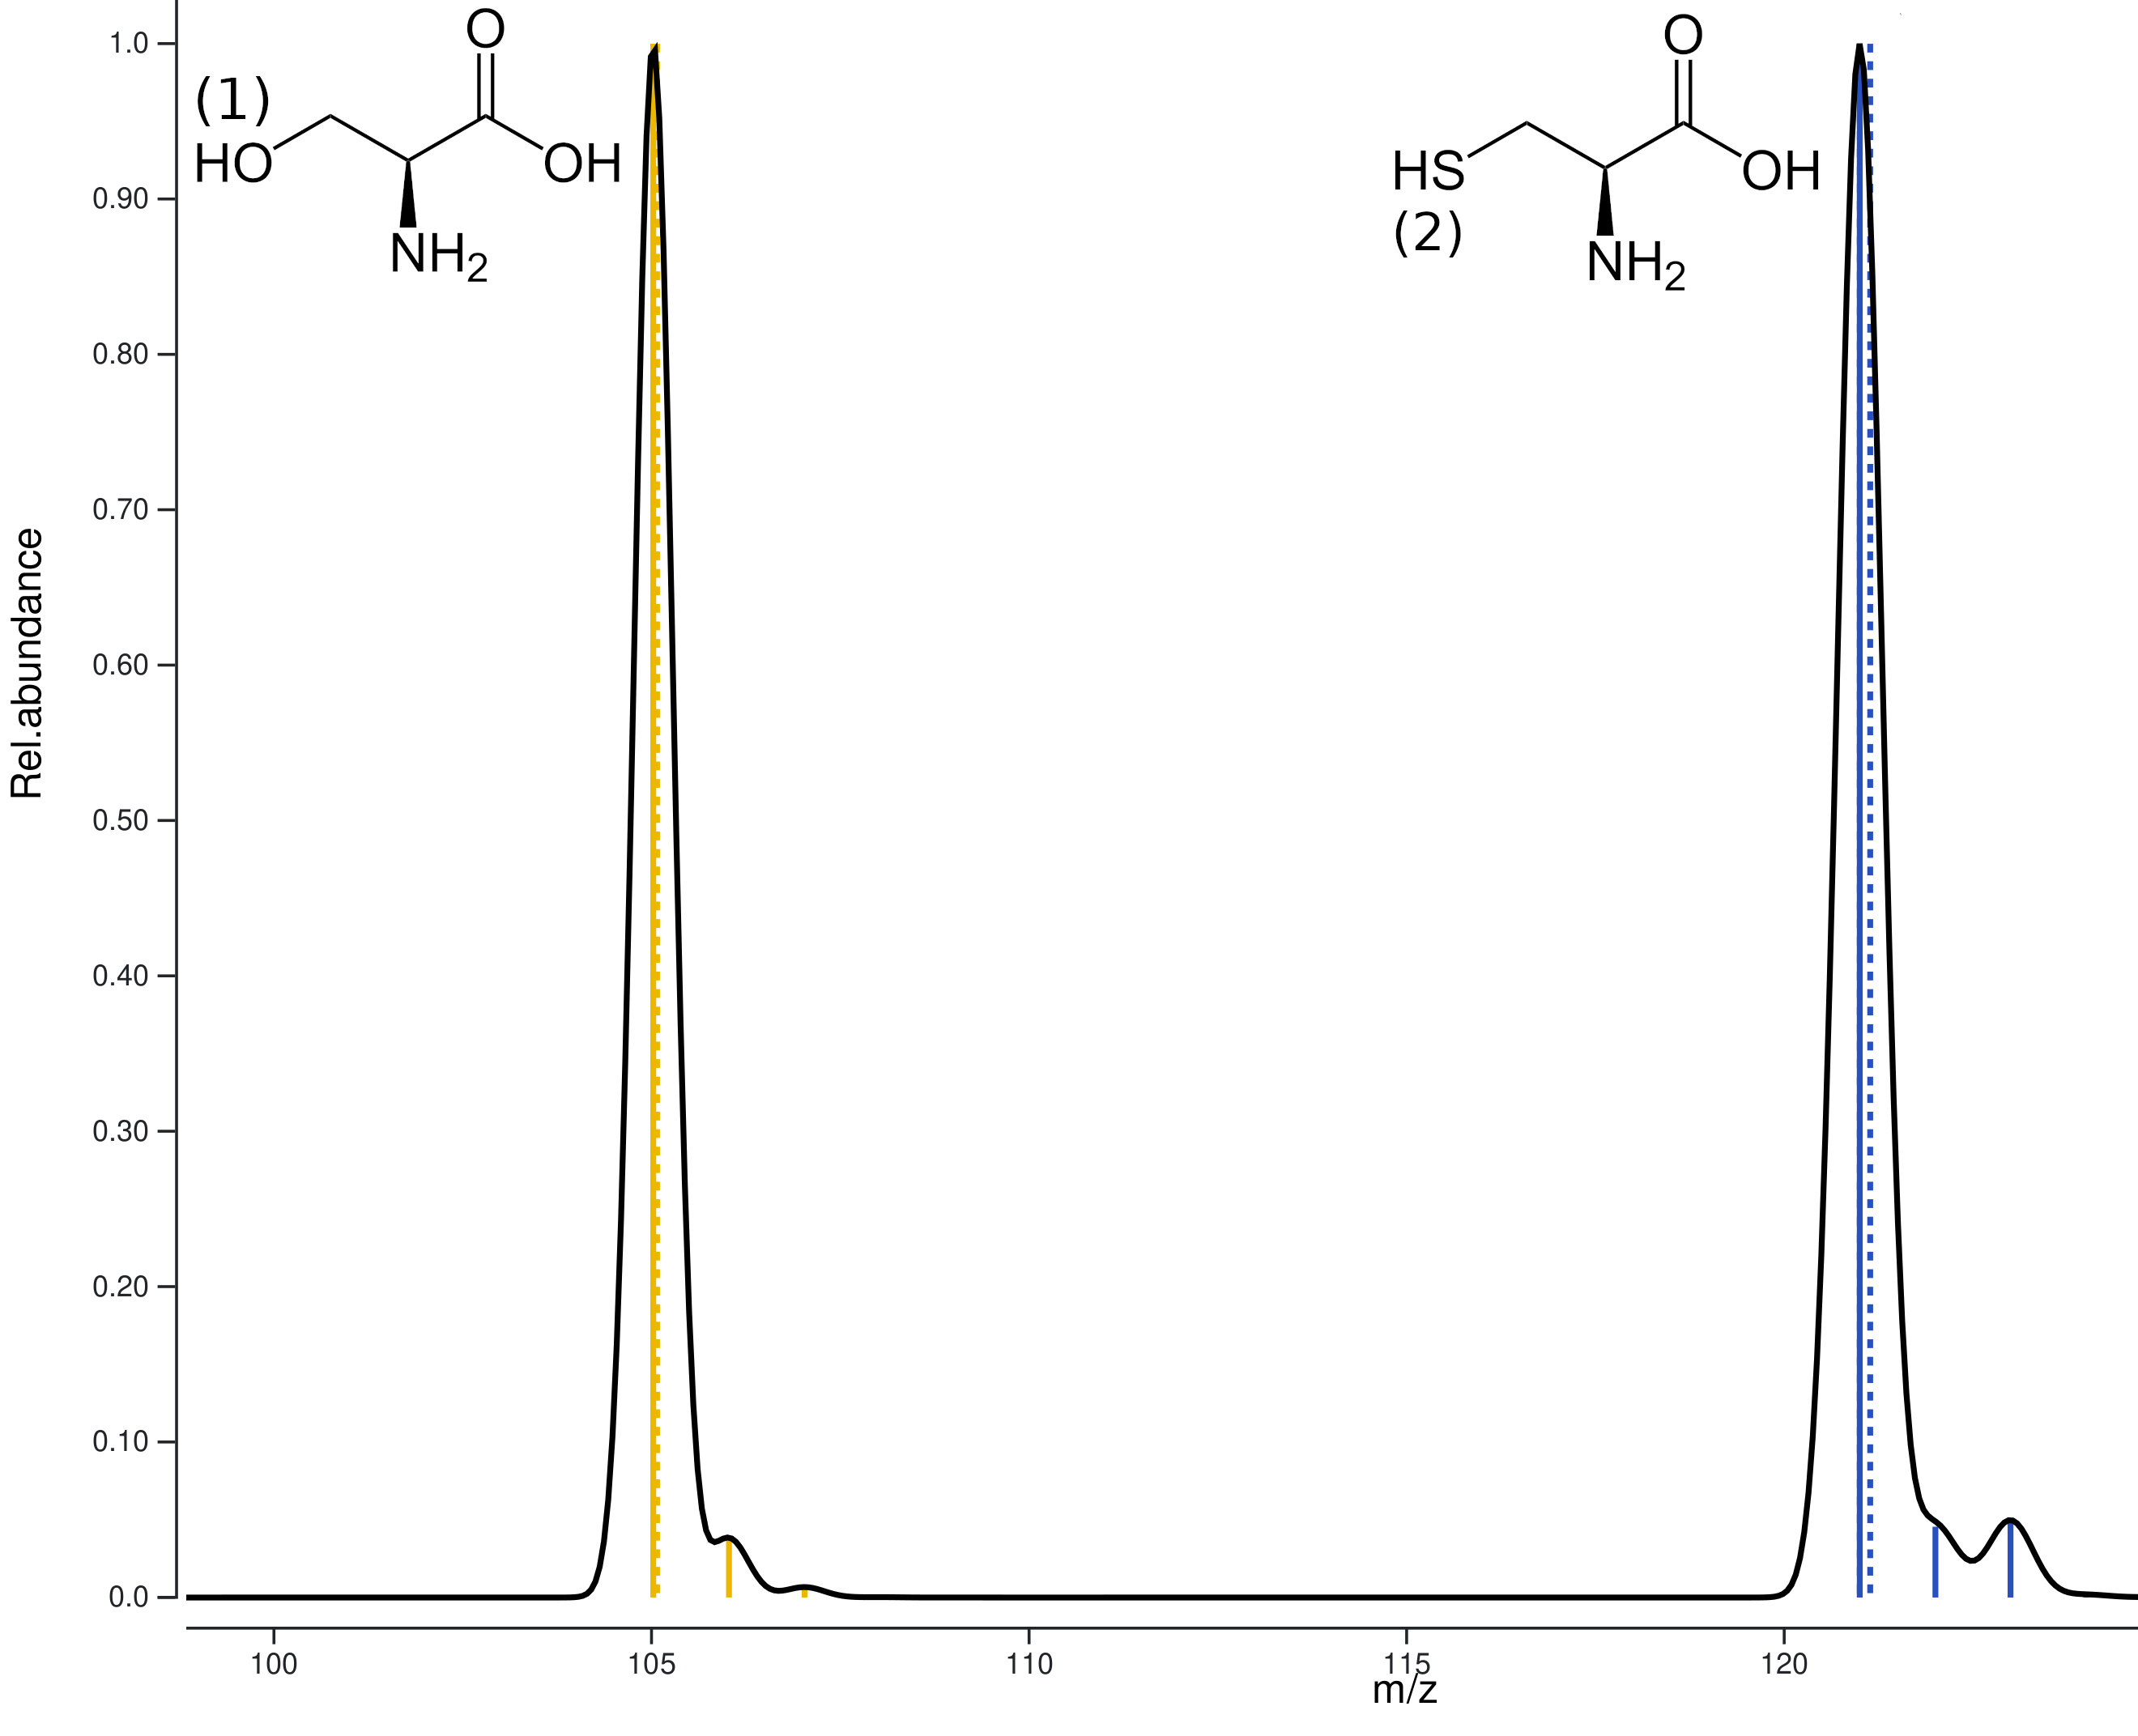
\includegraphics[width=0.75\textwidth]{./Resources/Simulated_Mass_Spectrum.png}
   \centering
   \caption{Computergeneriertes Massenspektrum von der Aminosäure \emph{Serin} (1) und \emph{Cystesin} (2). Peak von \emph{Serin} liegt bei 105; bei \emph{Systesin} um 121. y: relative Häufigkeit}
\end{figure}

Die Maxima werden \gerquot{Peaks} genannt und sind für eine Aminosäure an charakteristischer Position auf der $ x $-Achse. Obwohl sich die beiden Aminosäuren in der Abbildung \ref{fig:Sim_Mass_Spec} nur durch ein Atom unterscheiden (das linke Sauerstoffatom wurde durch ein Schwefelatom ersetzt) sind deren Massenspektren auf der $ x $-Achse weit voneinander entfernt und machen die beiden Aminosäuren dadurch sicher unterscheidbar.\\

Bei einzelnen Aminosäuren funktioniert die MS zuverlässig; bei Peptiden allerdings steht man vor dem Problem, dass das Massenspektrum unübersichtlicher wird und auch Peaks, die von Hintergrundrauschen stammen, schwerer herausgefiltert werden können. Abhilfe schafft hier die Tandem-Massenspektrometrie.

\subsection{Tandem-Massenspektrometrie (MS/MS)}\label{ss:Tandem_MS}
Bei der Tandem-Massenspektrometrie (MS/MS oder MS2) werden zwei MS Vorgänge hintereinander mit einer Probe durchgeführt. Die erste MS dient dazu Ionen aus einem bestimmten \massCharge Bereich auswählbar zu machen. Es entspricht also quasi einer Form der Filterung.

Vor der 2. MS werden die ausgewählten Reste einer Fragmentierung unterzogen. Bei einer Fragmentierung führt man Energie zu mit dem Ziel, dass die Ionen zerfallen und sog. Fragment-Ionen bilden. Diese Fragment-Ionen werden dann auf dem Massenspektrum nach der 2. MS sichtbar gemacht.

Fragment-Ionen sind kleiner als die ursprünglichen Ionen. So kann die 2. MS mit einer höheren Selektivität durchgeführt werden, welches Peaks durch Hintergrundrauschen verringert. Auch lassen sich Ionen besser identifizieren, die ein sehr ähnliches \massCharge-Verhältnis besitzen. Nach der 2. MS liegt eine Fülle an Fragment-Ionen-Peaks vor, aus denen sich die ursprünglichen Strukturinformationen ableiten lassen, da Ionen in spezifische Fragmente zerfallen \cite{Gross2013}. Zusammengefasst kann man sagen, dass das MS/MS Verfahren Ergebnisse höherer Güte erzeugt im Vergleich zur einfachen MS.

\section{De-Novo-Peptidsequenzierung mit \emph{pNovo+}}\label{s:pNovoPlusSeq}
Die \emph{pNovo+} Methode ist eine \gls{gls:DeNovo}, die mit einem \gls{gls:SpecGraph}en für die Auswertung der MS2-Spektren arbeitet und eine Erweiterung des \emph{pNovo} Verfahren darstellt \cite{pNovo}. Der Hauptansatz ist, dass zwei MS/MS Durchläufe mit jeweils verschiedenen Fragmentierungsmethoden\footnote{\emph{pNovo+} verwendet die higher energy
collisional dissociation (HCD) und die electron transfer dissociation (ETD) Fragmentierungsmethoden.} durchgeführt werden. Durch die Wahl einer anderen Fragmentierungsmethode ändert sich auch das MS2-Spektrum. Wenn nun Fragmentierungsmethoden verwendet werden, die möglichst komplementäre Spektren erzeugen, dann lässt sich durch das Zusammenführen der beiden MS2-Spektren die Qualität der Ergebnisse verbessern. Zum Beispiel lassen sich dadurch viele Peaks, die vom Hintergrundrauschen stammen, entfernen.

Für die Ermittlung der Sequenz eines Peptides wird zunächst ein Spektrums-Graph gebildet \dashAndSpace in Form eines DAG (directed acyclic graph). In diesem Graphen wird dann der längste Pfad bei gegebenen Start- und Endknoten berechnet. Die Reihenfolge der Knoten, die im längsten Pfad durchlaufen werden, stellt dann die Peptidsequenz dar.

\subsection{Vorverarbeitung der MS2-Spektren}\label{ss:Vorverarbeitung}
Bevor aus den MS2-Spektren der Spektrums-Graph gebildet werden kann, müssen die Daten vorverarbeitet werden. Für die Auswertung ist es von entscheidener Bedeutung, dass möglichst wenig Peaks verwendet werden, die vom Hintergrundrauschen stammen. Im weiteren Verlauf werden an einem exemplarischen MS2-Spektrum die Verarbeitungsschritte dargestellt.\\

Der erste Schritt ist das Verwenden des natürlichen Logarithmus der Intensitäten. Die Idee dabei ist, dass Hintergrundrauschen nicht überpriorisiert wird.

\begin{figure}[H]
   \centering
   \begin{minipage}[t]{.45\linewidth}
      \centering
      \begin{tikzpicture}[scale=\tikzScale, baseline=(current bounding box.center)]
         \draw [<->,thick] (0,\yAxisHeight) node (yaxis) [above] {\yAxisUnit}
         |- (\xAxisLength,0) node (xaxis) [right] {\xAxisUnit};
\draw[thick] (0.2, 0.0) -- (0.2, 2.3);
\draw[thick] (0.382, 0.0) -- (0.382, 1.7);
\draw[thick] (0.476, 0.0) -- (0.476, 2.7);
\draw[thick] (0.456, 0.0) -- (0.456, 1.8);
\draw[thick] (0.6859999999999999, 0.0) -- (0.6859999999999999, 2.7);
\draw[thick] (0.6839999999999999, 0.0) -- (0.6839999999999999, 1.8);
\draw[thick] (0.752, 0.0) -- (0.752, 1.1);
\draw[thick] (0.8200000000000001, 0.0) -- (0.8200000000000001, 2.2);
\draw[thick] (1.076, 0.0) -- (1.076, 1.5);
\draw[thick] (1.16, 0.0) -- (1.16, 1.9);
\draw[thick] (1.2120000000000002, 0.0) -- (1.2120000000000002, 2.0);
\draw[thick] (1.28, 0.0) -- (1.28, 1.9);
\draw[thick] (1.452, 0.0) -- (1.452, 1.3);
\draw[thick] (1.426, 0.0) -- (1.426, 1.9);
\draw[thick] (1.548, 0.0) -- (1.548, 1.9);
\draw[thick] (1.6740000000000002, 0.0) -- (1.6740000000000002, 1.5);
\draw[thick] (1.788, 0.0) -- (1.788, 2.5);
\draw[thick] (1.856, 0.0) -- (1.856, 2.3);
\draw[thick] (2.036, 0.0) -- (2.036, 1.7);
\draw[thick] (2.142, 0.0) -- (2.142, 1.6);
\draw[thick] (2.2520000000000002, 0.0) -- (2.2520000000000002, 2.0);
\draw[thick] (2.386, 0.0) -- (2.386, 1.6);
\draw[thick] (2.488, 0.0) -- (2.488, 2.9);
\draw[thick] (2.4739999999999998, 0.0) -- (2.4739999999999998, 2.7);
\draw[thick] (2.504, 0.0) -- (2.504, 2.0);
\draw[thick] (2.682, 0.0) -- (2.682, 2.0);
\draw[thick] (2.702, 0.0) -- (2.702, 2.5);
\draw[thick] (2.9259999999999997, 0.0) -- (2.9259999999999997, 2.8);
\draw[thick] (3.024, 0.0) -- (3.024, 2.4);
\draw[thick] (3.096, 0.0) -- (3.096, 1.8);
\draw[thick] (3.244, 0.0) -- (3.244, 2.6);
\draw[thick] (3.362, 0.0) -- (3.362, 1.9);
\draw[thick] (3.46, 0.0) -- (3.46, 2.3);
\draw[thick] (3.516, 0.0) -- (3.516, 1.1);
\draw[thick] (3.584, 0.0) -- (3.584, 1.8);
\draw[thick] (3.652, 0.0) -- (3.652, 2.0);
\draw[thick] (3.838, 0.0) -- (3.838, 1.5);
\draw[thick] (3.8819999999999997, 0.0) -- (3.8819999999999997, 2.6);
\draw[thick] (4.088, 0.0) -- (4.088, 2.6);
\draw[thick] (4.046, 0.0) -- (4.046, 1.1);
\draw[thick] (4.167999999999999, 0.0) -- (4.167999999999999, 2.0);
\draw[thick] (4.266, 0.0) -- (4.266, 2.4);
\draw[thick] (4.38, 0.0) -- (4.38, 1.1);
\draw[thick] (4.456, 0.0) -- (4.456, 2.2);
\draw[thick] (4.644, 0.0) -- (4.644, 2.6);
\draw[thick] (4.675999999999999, 0.0) -- (4.675999999999999, 2.5);
\draw[thick] (4.898000000000001, 0.0) -- (4.898000000000001, 1.2);
   \end{tikzpicture}%
   \end{minipage}%
   \textbf{$\rightarrow$} 
   \begin{minipage}[t]{.45\linewidth}
      \centering
      \begin{tikzpicture}[scale=\tikzScale, baseline=(current bounding box.center)]
      \draw [<->,thick] (0,\yAxisHeight) node (yaxis) [above] {\yAxisUnit}
      |- (\xAxisLength,0) node (xaxis) [right] {\xAxisUnit};
\draw[thick] (0.2, 0.0) -- (0.2, {ln(2.3)});
\draw[thick] (0.382, 0.0) -- (0.382, {ln(1.7)});
\draw[thick] (0.476, 0.0) -- (0.476, {ln(2.7)});
\draw[thick] (0.456, 0.0) -- (0.456, {ln(1.8)});
\draw[thick] (0.6859999999999999, 0.0) -- (0.6859999999999999, {ln(2.7)});
\draw[thick] (0.6839999999999999, 0.0) -- (0.6839999999999999, {ln(1.8)});
\draw[thick] (0.752, 0.0) -- (0.752, {ln(1.1)});
\draw[thick] (0.8200000000000001, 0.0) -- (0.8200000000000001, {ln(2.2)});
\draw[thick] (1.076, 0.0) -- (1.076, {ln(1.5)});
\draw[thick] (1.16, 0.0) -- (1.16, {ln(1.9)});
\draw[thick] (1.2120000000000002, 0.0) -- (1.2120000000000002, {ln(2.0)});
\draw[thick] (1.28, 0.0) -- (1.28, {ln(1.9)});
\draw[thick] (1.452, 0.0) -- (1.452, {ln(1.3)});
\draw[thick] (1.426, 0.0) -- (1.426, {ln(1.9)});
\draw[thick] (1.548, 0.0) -- (1.548, {ln(1.9)});
\draw[thick] (1.6740000000000002, 0.0) -- (1.6740000000000002, {ln(1.5)});
\draw[thick] (1.788, 0.0) -- (1.788, {ln(2.5)});
\draw[thick] (1.856, 0.0) -- (1.856, {ln(2.3)});
\draw[thick] (2.036, 0.0) -- (2.036, {ln(1.7)});
\draw[thick] (2.142, 0.0) -- (2.142, {ln(1.6)});
\draw[thick] (2.2520000000000002, 0.0) -- (2.2520000000000002, {ln(2.0)});
\draw[thick] (2.386, 0.0) -- (2.386, {ln(1.6)});
\draw[thick] (2.488, 0.0) -- (2.488, {ln(2.9)});
\draw[thick] (2.4739999999999998, 0.0) -- (2.4739999999999998, {ln(2.7)});
\draw[thick] (2.504, 0.0) -- (2.504, {ln(2.0)});
\draw[thick] (2.682, 0.0) -- (2.682, {ln(2.0)});
\draw[thick] (2.702, 0.0) -- (2.702, {ln(2.5)});
\draw[thick] (2.9259999999999997, 0.0) -- (2.9259999999999997, {ln(2.8)});
\draw[thick] (3.024, 0.0) -- (3.024, {ln(2.4)});
\draw[thick] (3.096, 0.0) -- (3.096, {ln(1.8)});
\draw[thick] (3.244, 0.0) -- (3.244, {ln(2.6)});
\draw[thick] (3.362, 0.0) -- (3.362, {ln(1.9)});
\draw[thick] (3.46, 0.0) -- (3.46, {ln(2.3)});
\draw[thick] (3.516, 0.0) -- (3.516, {ln(1.1)});
\draw[thick] (3.584, 0.0) -- (3.584, {ln(1.8)});
\draw[thick] (3.652, 0.0) -- (3.652, {ln(2.0)});
\draw[thick] (3.838, 0.0) -- (3.838, {ln(1.5)});
\draw[thick] (3.8819999999999997, 0.0) -- (3.8819999999999997, {ln(2.6)});
\draw[thick] (4.088, 0.0) -- (4.088, {ln(2.6)});
\draw[thick] (4.046, 0.0) -- (4.046, {ln(1.1)});
\draw[thick] (4.167999999999999, 0.0) -- (4.167999999999999, {ln(2.0)});
\draw[thick] (4.266, 0.0) -- (4.266, {ln(2.4)});
\draw[thick] (4.38, 0.0) -- (4.38, {ln(1.1)});
\draw[thick] (4.456, 0.0) -- (4.456, {ln(2.2)});
\draw[thick] (4.644, 0.0) -- (4.644, {ln(2.6)});
\draw[thick] (4.675999999999999, 0.0) -- (4.675999999999999, {ln(2.5)});
\draw[thick] (4.898000000000001, 0.0) -- (4.898000000000001, {ln(1.2)});
      \end{tikzpicture}
      \end{minipage}
      \caption{Anwendung des $ ln $ auf einem exemplarischen MS2-Spektrum.}
\end{figure}

Für das Verständnis des nächsten Schrittes muss man sich in Erinnerung rufen, dass eine gleiche Aminosäure keineswegs immer die gleiche Masse hat. Durch Isotope existiert eine gewisse \gerquot{Massenbandbreite} für ein und dieselbe Aminosäure. MS Systeme sind heute so genau, dass sie diese Differenzen erkennen. Dies hat den ungewollten Effekt, dass mehrere Peaks zu einer Aminosäure gehören können \cite{IsotopicDistributionMS}. Gleichzeitig können die \gerquot{Massenbandbreiten} zweier Aminosäuren sich überschneiden, sodass im ungünstigen Fall zwei Peaks kaum unterscheidbar nebeneinander liegen.\\

Eine Möglichkeit mit dieser Problematik umzugehen ist die Verwendung der monoisotopischen Masse. Die monoisotopische Masse ist die \gerquot{[...] exact mass of the most abundant naturally occurring stable isotope determined relative to the mass of 12 C, which is assigned the exact value of 12.0000.} \cite{MonoisotopicMass}. Ohne dabei jetzt tiefer ins Detail zu gehen kann man sagen, dass alle Peaks, deren Intensität mit einer möglichen monoisotopischen Masse übereinstimmen, auf jeden Fall einer Aminosäure entsprechen und (höchstwahrscheinlich)\footnote{Natürlich ist es möglich, dass das Rauschen zufällig einer monoisotopischen Masse entspricht. Die Wahrscheinlichkeit dafür ist allerdings sehr gering.} kein Hintergrundrauschen sind \cite{MassDefectMS}. Diese Peaks bekommen eine sogennante \emph{charge state}.\\

Der Algorithmus verwendet die \emph{charge state} Peaks als Ausganspunkte für weitere Berechnungen. Wenn die \massCharge Differenz zu einem anderen Peak einem Peptidfragment entspricht, dann stammt dieser Peak höchstwahrscheinlich von einem Fragment. Insgesamt werden damit die relevanten Peptidfragmente herausgeholt. Abbildung \ref{MonoisotopicMassFiltering} zeigt das Ergebnis nach den beiden zuvor genannten Schritten.

\begin{figure}[H]\label{MonoisotopicMassFiltering}
   \centering
   \begin{minipage}[t]{.45\linewidth}
      \centering
      \begin{tikzpicture}[scale=\tikzScale, baseline=(current bounding box.center)]
         \draw [<->,thick] (0,\yAxisHeight) node (yaxis) [above] {\yAxisUnit}
         |- (\xAxisLength,0) node (xaxis) [right] {\xAxisUnit};
\draw[thick] (0.2, 0.0) -- (0.2, {ln(2.3)});
\draw[color=blue!85!,opacity=.55,thick] (0.382, 0.0) -- (0.382, {ln(1.7)});
\draw[color=blue!85!,opacity=.55,thick] (0.476, 0.0) -- (0.476, {ln(2.7)});
\draw[color=magenta,thick] (0.456, 0.0) -- (0.456, {ln(1.8)});
\draw[color=blue!85!,opacity=.55,thick] (0.6859999999999999, 0.0) -- (0.6859999999999999, {ln(2.7)});
\draw[color=blue!85!,opacity=.55,thick] (0.6839999999999999, 0.0) -- (0.6839999999999999, {ln(1.8)});
\draw[thick] (0.752, 0.0) -- (0.752, {ln(1.1)});
\draw[thick] (0.8200000000000001, 0.0) -- (0.8200000000000001, {ln(2.2)});
\draw[thick] (1.076, 0.0) -- (1.076, {ln(1.5)});
\draw[thick] (1.16, 0.0) -- (1.16, {ln(1.9)});
\draw[thick] (1.2120000000000002, 0.0) -- (1.2120000000000002, {ln(2.0)});
\draw[thick] (1.28, 0.0) -- (1.28, {ln(1.9)});
\draw[color=blue!85!,opacity=.55,thick] (1.452, 0.0) -- (1.452, {ln(1.3)});
\draw[color=blue!85!,opacity=.55,thick] (1.426, 0.0) -- (1.426, {ln(1.9)});
\draw[color=magenta,thick] (1.548, 0.0) -- (1.548, {ln(1.9)});
\draw[color=blue!85!,opacity=.55,thick] (1.6740000000000002, 0.0) -- (1.6740000000000002, {ln(1.5)});
\draw[color=blue!85!,opacity=.55,thick] (1.788, 0.0) -- (1.788, {ln(2.5)});
\draw[thick] (1.856, 0.0) -- (1.856, {ln(2.3)});
\draw[thick] (2.036, 0.0) -- (2.036, {ln(1.7)});
\draw[thick] (2.142, 0.0) -- (2.142, {ln(1.6)});
\draw[thick] (2.2520000000000002, 0.0) -- (2.2520000000000002, {ln(2.0)});
\draw[thick] (2.386, 0.0) -- (2.386, {ln(1.6)});
\draw[color=blue!85!,opacity=.55,thick] (2.488, 0.0) -- (2.488, {ln(2.9)});
\draw[thick] (2.4739999999999998, 0.0) -- (2.4739999999999998, {ln(2.7)});
\draw[color=blue!85!,opacity=.55,thick] (2.504, 0.0) -- (2.504, {ln(2.0)});
\draw[color=magenta,thick] (2.682, 0.0) -- (2.682, {ln(2.0)});
\draw[color=blue!85!,opacity=.55,thick] (2.702, 0.0) -- (2.702, {ln(2.5)});
\draw[thick] (2.9259999999999997, 0.0) -- (2.9259999999999997, {ln(2.8)});
\draw[thick] (3.024, 0.0) -- (3.024, {ln(2.4)});
\draw[thick] (3.096, 0.0) -- (3.096, {ln(1.8)});
\draw[thick] (3.244, 0.0) -- (3.244, {ln(2.6)});
\draw[thick] (3.362, 0.0) -- (3.362, {ln(1.9)});
\draw[color=blue!85!,opacity=.55,thick] (3.46, 0.0) -- (3.46, {ln(2.3)});
\draw[color=blue!85!,opacity=.55,thick] (3.516, 0.0) -- (3.516, {ln(1.1)});
\draw[color=blue!85!,opacity=.55,thick] (3.584, 0.0) -- (3.584, {ln(1.8)});
\draw[color=magenta,thick] (3.652, 0.0) -- (3.652, {ln(2.0)});
\draw[color=blue!85!,opacity=.55,thick] (3.838, 0.0) -- (3.838, {ln(1.5)});
\draw[color=blue!85!,opacity=.55,thick] (3.8819999999999997, 0.0) -- (3.8819999999999997, {ln(2.6)});
\draw[thick] (4.088, 0.0) -- (4.088, {ln(2.6)});
\draw[thick] (4.046, 0.0) -- (4.046, {ln(1.1)});
\draw[thick] (4.167999999999999, 0.0) -- (4.167999999999999, {ln(2.0)});
\draw[thick] (4.266, 0.0) -- (4.266, {ln(2.4)});
\draw[color=blue!85!,opacity=.55,thick] (4.38, 0.0) -- (4.38, {ln(1.1)});
\draw[color=blue!85!,opacity=.55,thick] (4.456, 0.0) -- (4.456, {ln(2.2)});
\draw[color=magenta,thick] (4.644, 0.0) -- (4.644, {ln(2.6)});
\draw[color=blue!85!,opacity=.55,thick] (4.675999999999999, 0.0) -- (4.675999999999999, {ln(2.5)});
\draw[color=blue!85!,opacity=.55,thick] (4.898000000000001, 0.0) -- (4.898000000000001, {ln(1.2)});
   \end{tikzpicture}%
   \end{minipage}%
   \textbf{$\rightarrow$} 
   \begin{minipage}[t]{.45\linewidth}
      \centering
      \begin{tikzpicture}[scale=\tikzScale, baseline=(current bounding box.center)]
      \draw [<->,thick] (0,\yAxisHeight) node (yaxis) [above] {\yAxisUnit}
      |- (\xAxisLength,0) node (xaxis) [right] {\xAxisUnit};
\draw[color=blue!85!,opacity=.55,thick] (0.382, 0.0) -- (0.382, {ln(1.7)});
\draw[color=blue!85!,opacity=.55,thick] (0.476, 0.0) -- (0.476, {ln(2.7)});
\draw[color=magenta,thick] (0.456, 0.0) -- (0.456, {ln(1.8)});
\draw[color=blue!85!,opacity=.55,thick] (0.6859999999999999, 0.0) -- (0.6859999999999999, {ln(2.7)});
\draw[color=blue!85!,opacity=.55,thick] (0.6839999999999999, 0.0) -- (0.6839999999999999, {ln(1.8)});
\draw[color=blue!85!,opacity=.55,thick] (1.452, 0.0) -- (1.452, {ln(1.3)});
\draw[color=blue!85!,opacity=.55,thick] (1.426, 0.0) -- (1.426, {ln(1.9)});
\draw[color=magenta,thick] (1.548, 0.0) -- (1.548, {ln(1.9)});
\draw[color=blue!85!,opacity=.55,thick] (1.6740000000000002, 0.0) -- (1.6740000000000002, {ln(1.5)});
\draw[color=blue!85!,opacity=.55,thick] (1.788, 0.0) -- (1.788, {ln(2.5)});
\draw[color=blue!85!,opacity=.55,thick] (2.488, 0.0) -- (2.488, {ln(2.9)});
\draw[color=blue!85!,opacity=.55,thick] (2.504, 0.0) -- (2.504, {ln(2.0)});
\draw[color=magenta,thick] (2.682, 0.0) -- (2.682, {ln(2.0)});
\draw[color=blue!85!,opacity=.55,thick] (2.702, 0.0) -- (2.702, {ln(2.5)});
\draw[color=blue!85!,opacity=.55,thick] (3.46, 0.0) -- (3.46, {ln(2.3)});
\draw[color=blue!85!,opacity=.55,thick] (3.516, 0.0) -- (3.516, {ln(1.1)});
\draw[color=blue!85!,opacity=.55,thick] (3.584, 0.0) -- (3.584, {ln(1.8)});
\draw[color=magenta,thick] (3.652, 0.0) -- (3.652, {ln(2.0)});
\draw[color=blue!85!,opacity=.55,thick] (3.838, 0.0) -- (3.838, {ln(1.5)});
\draw[color=blue!85!,opacity=.55,thick] (3.8819999999999997, 0.0) -- (3.8819999999999997, {ln(2.6)});
\draw[color=blue!85!,opacity=.55,thick] (4.38, 0.0) -- (4.38, {ln(1.1)});
\draw[color=blue!85!,opacity=.55,thick] (4.456, 0.0) -- (4.456, {ln(2.2)});
\draw[color=magenta,thick] (4.644, 0.0) -- (4.644, {ln(2.6)});
\draw[color=blue!85!,opacity=.55,thick] (4.675999999999999, 0.0) -- (4.675999999999999, {ln(2.5)});
\draw[color=blue!85!,opacity=.55,thick] (4.898000000000001, 0.0) -- (4.898000000000001, {ln(1.2)});
      \end{tikzpicture}
      \end{minipage}
      \caption{Entfernen von Peaks, die keiner monoisotopischen Masse entsprechen oder benachbart mit einer Differenz von einem Fragment-Ion sind.}
\end{figure}

Tatsächlich ist die Verarbeitung an dieser Stelle noch etwas komplexer. So existieren auch noch sogenannte \emph{isotopic cluster}\footnote{Definition eines \emph{isotopic cluster} nach IUPAC: \gerquot{Group of peaks representing ions of the same elemental composition, but different isotopic compositions.} \cite[1556]{IUPACDefinitions}}, die gesondert verarbeitet werden. Für das grundsätzliche Prinzip ist dieses Detail allerdings weniger relevant.\\

Im letzten Vorberarbeitungsschritt werden Peaks aus einem irrelevanten \massCharge Bereich entfernt und naheliegende Peaks werden zusammengefasst, indem der Mittelwert sowol des \massCharge Wertes als auch der der Intensität besimmt wird. Üblicherweise liegt der Bereich für das Zusammenfassen bei $ +- 20 ppm $.

\begin{figure}[H]
   \centering
   \begin{minipage}[t]{.45\linewidth}
      \centering
      \begin{tikzpicture}[scale=\tikzScale, baseline=(current bounding box.center)]
         \draw [<->,thick] (0,\yAxisHeight) node (yaxis) [above] {\yAxisUnit}
         |- (\xAxisLength,0) node (xaxis) [right] {\xAxisUnit};
\draw[thick] (0.382, 0.0) -- (0.382, {ln(1.7)});
\draw[thick] (0.476, 0.0) -- (0.476, {ln(2.7)});
\draw[thick] (0.456, 0.0) -- (0.456, {ln(1.8)});
\draw[thick] (0.6859999999999999, 0.0) -- (0.6859999999999999, {ln(2.7)});
\draw[thick] (0.6839999999999999, 0.0) -- (0.6839999999999999, {ln(1.8)});
\draw[color=red,thick] (1.452, 0.0) -- (1.452, {ln(1.3)});
\draw[color=red,thick] (1.426, 0.0) -- (1.426, {ln(1.9)});
\draw[thick] (1.548, 0.0) -- (1.548, {ln(1.9)});
\draw[thick] (1.6740000000000002, 0.0) -- (1.6740000000000002, {ln(1.5)});
\draw[thick] (1.788, 0.0) -- (1.788, {ln(2.5)});
\draw[color=red,thick] (2.488, 0.0) -- (2.488, {ln(2.9)});
\draw[color=red,thick] (2.504, 0.0) -- (2.504, {ln(2.0)});
\draw[color=red,thick] (2.682, 0.0) -- (2.682, {ln(2.0)});
\draw[color=red,thick] (2.702, 0.0) -- (2.702, {ln(2.5)});
\draw[thick] (3.46, 0.0) -- (3.46, {ln(2.3)});
\draw[thick] (3.516, 0.0) -- (3.516, {ln(1.1)});
\draw[thick] (3.584, 0.0) -- (3.584, {ln(1.8)});
\draw[thick] (3.652, 0.0) -- (3.652, {ln(2.0)});
\draw[color=red,thick] (3.838, 0.0) -- (3.838, {ln(1.5)});
\draw[color=red,thick] (3.8819999999999997, 0.0) -- (3.8819999999999997, {ln(2.6)});
\draw[thick] (4.38, 0.0) -- (4.38, {ln(1.1)});
\draw[thick] (4.456, 0.0) -- (4.456, {ln(2.2)});
\draw[thick] (4.644, 0.0) -- (4.644, {ln(2.6)});
\draw[thick] (4.675999999999999, 0.0) -- (4.675999999999999, {ln(2.5)});
\draw[thick] (4.898000000000001, 0.0) -- (4.898000000000001, {ln(1.2)});

\fill[red!25!,opacity=.25] (0,0) rectangle (1,\yAxisHeight-\axisColorOffset);
         \fill[red!25!,opacity=.25] (\xAxisLength-1,0) rectangle (\xAxisLength-\axisColorOffset,\yAxisHeight-\axisColorOffset);
         \fill[green!25!,opacity=.25] (1,0) rectangle (\xAxisLength-1,\yAxisHeight-\axisColorOffset);
   \end{tikzpicture}%
   \end{minipage}%
   \textbf{$\rightarrow$} 
   \begin{minipage}[t]{.45\linewidth}
      \centering
      \begin{tikzpicture}[scale=\tikzScale, baseline=(current bounding box.center)]
      \draw [<->,thick] (0,\yAxisHeight) node (yaxis) [above] {\yAxisUnit}
      |- (\xAxisLength,0) node (xaxis) [right] {\xAxisUnit};
%\draw[color=red,thick] (1.452, 0.0) -- (1.452, {ln(1.3)});
%\draw[color=red,thick] (1.426, 0.0) -- (1.426, {ln(1.9)});
\draw[color=red,ultra thick] ({(1.452+1.426)/2}, 0.0) -- ({(1.452+1.426)/2}, {(ln(1.3)+ln(1.9))/2});

\draw[thick] (1.548, 0.0) -- (1.548, {ln(1.9)});
\draw[thick] (1.6740000000000002, 0.0) -- (1.6740000000000002, {ln(1.5)});
\draw[thick] (1.788, 0.0) -- (1.788, {ln(2.5)});

%\draw[color=red,thick] (2.488, 0.0) -- (2.488, {ln(2.9)});
%\draw[color=red,thick] (2.504, 0.0) -- (2.504, {ln(2.0)});
\draw[color=red,ultra thick] ({(2.488+2.504)/2}, 0.0) -- ({(2.488+2.504)/2}, {(ln(2.9)+ln(2.0))/2});

%\draw[color=red,thick] (2.682, 0.0) -- (2.682, {ln(2.0)});
%\draw[color=red,thick] (2.702, 0.0) -- (2.702, {ln(2.5)});
\draw[color=red,ultra thick] ({(2.682+2.702)/2}, 0.0) -- ({(2.682+2.702)/2}, {(ln(2.0+ln(2.5))/2});

\draw[thick] (3.46, 0.0) -- (3.46, {ln(2.3)});
\draw[thick] (3.516, 0.0) -- (3.516, {ln(1.1)});
\draw[thick] (3.584, 0.0) -- (3.584, {ln(1.8)});
\draw[thick] (3.652, 0.0) -- (3.652, {ln(2.0)});

%\draw[color=red,thick] (3.838, 0.0) -- (3.838, {ln(1.5)});
%\draw[color=red,thick] (3.8819999999999997, 0.0) -- (3.8819999999999997,{ln(2.6)});
\draw[color=red,ultra thick] ({(3.838+3.8819999999999997)/2}, 0.0) -- ({(3.838+3.8819999999999997)/2}, {(ln(1.5)+ln(2.6))/2});

\fill[red!25!,opacity=.25] (0,0) rectangle (1,\yAxisHeight-\axisColorOffset);
         \fill[red!25!,opacity=.25] (\xAxisLength-1,0) rectangle (\xAxisLength-\axisColorOffset,\yAxisHeight-\axisColorOffset);
         \fill[green!25!,opacity=.25] (1,0) rectangle (\xAxisLength-1,\yAxisHeight-\axisColorOffset);
      \end{tikzpicture}
      \end{minipage}
      \caption{Entfernen von Peaks aus einem irrelevanten \massCharge Bereich und zusammenfassen naheliegender Peaks. Rot markierte Peaks sind jene, die zusammengefasst werden.}
\end{figure}

\subsection{Bildung eines Spektrums-Graphen}\label{ss:BildungSpekGraph}
Der Spektrums-Graph wird aus einem vorverarbeiteten MS2-Spektrum (siehe Kapitel: \ref{ss:Vorverarbeitung}) gebildet. Im initialen Zustand werden die Peaks als Knoten interpretiert. Dazu kommt ein Start- und Endknoten. Jedem Knoten wird eine Masse zugeordet; im initialen Zustand bekommt der Startknoten die Masse 0 und der Endknoten die Masse des vorherigen Knotens minus der Masse des Wassers ($ 18,02 $). Die Masse der übrigen Knoten entsprechen ihren jeweils korrespondierenden \massCharge Wert. Die gerichteten Kanten werden zwischen einem Knotenpaar hinzugefügt, wenn die Differenz deren Masse gleich ist mit der Masse von ein oder zwei Aminosäuren.

\subsection{Identifikation der Aminosäuresequenz}
Der gebildete DAG kann mit klassischen Algorithmen, die den längsten Pfad suchen, durchlaufen werden. Bezogen auf die Graphentheorie entspricht die Ermittlung der Aminosäurensequenz dem Suchen eines bestimmten Pfades \dashAndSpace und nicht nach irgendeinem Pfad. Daher muss der Algorithmus mittels einer Breitensuche arbeiten, um alle möglichen Pfade zu bestimmen.

In aller Regel wird es mehrere Pfade geben. Bestimmte Sequenzen sind wahrscheinlicher als andere. So sind Pfade mit Kanten, die wegen der Massendifferenz von genau einer Aminosäure gebildet wurden, wahrscheinlicher \cite{pNovoPlus}. Alle Pfade bekommen mittels einer Scoring-Funktion einen Wert zugewiesen. Der Pfad mit dem höchsten Scoring-Wert ist wahrscheinlich das richtige Ergebnis. Die Scoring-Funktion berücksichtigt unter anderem wie viele Fragmente, die einer bestimmten Aminosäure zugeordet werden können, im MS2-Spektrum vorhanden sind \cite{pNovo}. Die Sequenz mit dem höchsten Scoring-Wert ist das Endergebnis.

\section{De-Novo-Peptidsequenzierung mit \emph{Open-pNovo}}\label{s:OpenpNovoSeq}
Bei Proteinen können posttranslationale Proteinmodifikationen (PTM) auftreten. PTMs sind Ereignisse, bei denen sich Änderungen im Protein einstellen \cite{Mann2003}; teilweise sind die Änderungen von einer Zelle erwünscht \dashAndSpace teilweise stammen sie aber auch zum Beispiel von unerwünschten Wechselwirkungen nebeneinanderliegenden Aminosäuren. Ein Teil dieser PTMs führen zu einer Änderung der Aminosäuresequenz. Dies ist für die \gls{gls:DeNovo} nicht weiter problematisch, da sowieso ohne eine Datenbank gearbeitet wird, sodass solche PTMs nicht einmal auffallen würden. Andere PTMs hingegen haben die Auswirkung, dass Stoffe gebildet werden, die nicht mehr zu der Gruppe der proteinogenen Aminosäuren gehören. Proteinogene Aminosäuren sind jene Aminosäuren, die für den Bau von Proteinen verwendet werden. Der Effekt ist also, dass Stoffe (oder deren Fragmente) bei einem Massenspektrum angezeigt werden, die kein Teil eines Peptids sein können. Bei der Sequenzierung von Peptidfragmenten muss dies daher berücksichtigt werden.
Wenn im weiteren Verlauf von PTMs gesprochen wird, dann sind solche gemeint, die für die \gls{gls:DeNovo} relevant sind.

Open-pNovo ist ein \gls{gls:DeNovo}sverfahren, welches auf pNovo+ Tool aufbaut und versucht die Problematik mit den PTMs zu lösen.

\subsection{PTMs im konstruierten DAG}
Die Konvertierung eines MS2-Spektrums läuft bis zum DAG analog ab wie in den Kapiteln \ref{ss:Vorverarbeitung} und \ref{ss:BildungSpekGraph} für pNovo+. Der Unterschied ist nun, dass es zwei Arten von Kanten gibt:

\begin{itemize}
   \item \gerquot{Normale} Kanten: Kanten, die gebildet werden, wie es bereits für \emph{pNovo+} gezeigt wurde. 
   \item \gerquot{Modifizierte} Kanten: Kanten, die zum Grahpen hinzugefügt werden, wenn die Massendifferenz zweier Knoten der Masse einer Aminosäure plus der Masse einer möglichen PTM-Änderung entspricht. 
\end{itemize}

Eine Liste aller PTMs in der Datenbank Unimod (sowohl relevante als auch nicht relevante) beinhaltet aktuell 1510 Einträge\footnote{Siehe: \url{https://www.ebi.ac.uk/ols/ontologies/unimod}} (Stand: 18.04.2022). Für die modifizierten Kanten gibt es insgesamt $ 1510 * 20 = 30200 $ mögliche Differenzen, wobei viele davon nicht relevante PTMs sind. Zum Vergleich: bei den normalen Kanten gibt es $ 20^2 = 400 $ mögliche Differenzen.

Die hohe Anzahl an Differenzen für modifizierte Kanten hat die Konsequenz, dass viele Knoten zufällig verbunden werden und dass dadurch die Genauigkeit der Ergebnisse abnimmt. Dieses Problem kann man durch eine geringere Liste an möglichen PTMs abfedern, allerdings mit einem Verlust  der Genauigkeit auf Seiten der PTMs. Es ist hier also eine Abwägung.

\subsection{Evaluierung von Open-pNovo}
Open-pNovo wurde sowohl auf drei realen als auch auf drei generierten Testdaten getestet. Tabelle \ref{tab:OpenPNovoResults} zeigt die Ergebnisse im Vergleich zu pNovo+ und zwei anderen Algorithmen. Die Datensätze enthielten die am häufigsten vorkommenden PTMs.

\begin{table}[H]
    \centering
    \begin{tabular}{l|c|c|c|c}
        \toprule
        \textbf{Testdatensätze} & \textbf{Open-pNovo+} & \textbf{pNovo+} & \textbf{PEAKS} & \textbf{Novor} \\
        \midrule
        Real (20259) & $76,3 \%$ & $68,5 \%$ & $65,8 \%$ & $39,9 \%$ \\
        Generiert (17877) & $77,8 \%$ & $0,6 \%$ & $0,5 \%$ & $0,2 \%$ \\
        \bottomrule
    \end{tabular}
    \newline
    \caption{Vergleich der durchschnittlichen richtigen \gls{gls:DeNovo} Peptidsequenzierungen von Open-pNovo und anderen Algorithmen \cite[650]{OpenPNovo}.}
    \label{tab:OpenPNovoResults}
\end{table}

Die enorm schlechten Ergebnisse der anderen Algorithmen bei den generierten Testdaten ist ein Nebeneffekt des Ziels bei der Testdatengenerierung. Denn diese wurden so ausgelegt, um die Grenzen von Open-pNovo+ zu ermitteln \cite[649]{OpenPNovo}. Eine Aussagekraft haben diese Ergebnisse also nicht. Allerdings auch bei realen Testdaten zeigt sich Open-pNovo als voll konkurrenzfähig gegenüber den anderen Algorithmen.

Noch besser zeigt sich Open-pNovo, wenn der Recall Wert betrachtet wird \dashAndSpace also die Anzahl an verschiedenen PSMs, die erkannt wurden. In diesem Fall ist der Abstand zu den anderen Algorithmen deutlich größer geworden.

\begin{table}[H]
    \centering
    \begin{tabular}{l|c|c|c|c}
        \toprule
        \textbf{Testdatensätze} & \textbf{Open-pNovo+} & \textbf{pNovo+} & \textbf{PEAKS} & \textbf{Novor} \\
        \midrule
        Real (5034) & $61,6 \%$ & $31,3 \%$ & $32,0 \%$ & $13,7 \%$ \\
        \bottomrule
    \end{tabular}
    \newline
    \caption{Vergleich der durchschnittlichen Recall Werte einer \gls{gls:DeNovo} Peptidsequenzierungen von Open-pNovo und anderen Algorithmen \cite[650]{OpenPNovo}.}
    \label{tab:OpenPNovoResultsRecall}
\end{table}

\subsection{Zusammenfassung}


% Die \gls{gls:DeNovo} nutzt die sogenannte \gls{gls:TMassSpek} für die Bestimmung der Peptidsequenz. Dabei wird die physikalische Eigenschaft ausgenutzt, dass jedes Atom bzw. jedes Molekül \dashAndSpace wenn es einer \gls{gls:Ionisation} unterzogen wurde \dashAndSpace ein charakteristisches \gls{gls:MassSpek} besitzt. Das \gls{gls:MassSpek} stellt also eine Art \gerquot{Fingerabdruck} eines Moleküls dar und macht dieses ermittelbar.

% U.U. eine Beispielgrafik eines Massenspektrums hinzufuegen ...

\subsubsection{\glsentrytext{gls:TMassSpek} bei größeren Molekülen}
Bei größeren Molekülen (wie einem Protein) führt die \gls{gls:Ionisation} dazu, dass das Molekül in kleinere spezifische Ionen zerfällt (sog. Fragmentierung). Die Fragmentierungsinformationen einer \gls{gls:DeNovo} sind meist unvollständig, da fehlende Daten bei einem Fragmentierungsschritt die Güte des Endergebnisses negativ beeinflusst. Dies wird insbesondere dann ein Problem, wenn unbekannte Änderungen in einer Peptidsequenz vorhanden sind.

Um dieses Problem zu verringern können unterschiedliche Techniken parallel eingesetzt werden, welche verschiedene Fragmente erzeugen und daher auch verschiedenartige \glspl{gls:MassSpek} zur Folge haben.\footnote{Konkret: Es wird sowohl das \gls{acr:HCD} als auch das \gls{acr:ETD} Verfahren angewendet.}

\subsection{Datenaufbereitung}
Typischerweise betrachtet man die sog. \gerquot{\glspl{gls:Peak}} in den \glspl{gls:MassSpek}. Jeder \gls{gls:Peak} stellt ein unterschiedliches Ion dar. Dazu kommen Messungenauigkeiten sowie Hintergrundrauschen. Durch die hohe Anzahl an möglichen Ionen kann nicht ohne weiteres differenziert werden, welcher der \glspl{gls:Peak} von welchen Ionen erzeugt wurden und welche nicht.

% Frage an Dominik: Ist hier eine einfache Auflistung an Techniken für die Datenaufbereitung besser?
Der Algorithmus für die Datenaufbereitung berechnet den natürlichen Logarithmus von den Intensitäten der \glspl{gls:Peak}, um Hintergrundrauschen und Messungenauigkeiten nicht überzupriorisieren. Zusätzlich dazu werden \glspl{gls:Peak}, die in einem Toleranzbereich nebeneinander liegen, zusammengefasst. Am Ende werden die \glspl{gls:Peak} entfernt, bei denen bekannt ist, dass es sich nicht um relevante Ionen handeln kann. (z.B. \glspl{gls:Peak} von Isotopen)

\begin{figure}[H]
   \centering
   \begin{minipage}[t]{.4\linewidth}
      \centering
      \begin{tikzpicture}[scale=\tikzScale, baseline=(current bounding box.center)]
         \draw [<->,thick] (0,2.75) node (yaxis) [above] {\yAxisUnit}
         |- (3,0) node (xaxis) [right] {\xAxisUnit};

         \draw[thick] (0.2,0) -- (0.2,1.1);
         \draw[thick] (0.3,0) -- (0.3,1.6);
         \draw[thick] (0.6,0) -- (0.6,1.7);
         \draw[thick] (0.8,0) -- (0.8,1.2);
         \draw[thick] (1.0,0) -- (1.0,1.1);

         \draw[color=red,thick] (1.2,0) -- (1.2,2.65);
         \draw[thick] (1.4,0) -- (1.4,1.4);
         \draw[thick] (1.6,0) -- (1.6,1.2);
         \draw[thick] (1.8,0) -- (1.8,1.3);
         \draw[thick] (2.0,0) -- (2.0,1.8);

         \draw[thick] (1.1,0) -- (1.1,2.0);
         \draw[color=red,thick] (0.35,0) -- (0.35,2.25);
         \draw[thick] (1.9,0) -- (1.9,1.4);
         \draw[color=red,thick] (2.2,0) -- (2.2,2.6);
         \draw[thick] (2.5,0) -- (2.5,1.25);

         \draw[thick] (2.7,0) -- (2.7,1.1);
         \foreach \x in {1,...,6}
         {
            \draw[thick] (1.2+\x*0.05,0) -- (1.2+\x*0.05,1.0+\x*0.15);
         }
      \end{tikzpicture}%
      % \subcaption{Exemplarische Rohdaten}
   \end{minipage}%
   \textbf{$\rightarrow$}
   \begin{minipage}[t]{.4\linewidth}
      \centering
      \begin{tikzpicture}[scale=\tikzScale, baseline=(current bounding box.center)]
         \draw [<->,thick] (0,2.75) node (yaxis) [above] {\yAxisUnit}
         |- (3,0) node (xaxis) [right] {\xAxisUnit};

         \draw[thick] (0.2,0) -- (0.2,{ln(1.1)});
         \draw[thick] (0.3,0) -- (0.3,{ln(1.6)});
         \draw[thick] (0.6,0) -- (0.6,{ln(1.7)});
         \draw[thick] (0.8,0) -- (0.8,{ln(1.2)});
         \draw[thick] (1.0,0) -- (1.0,{ln(1.1)});

         \draw[color=red,thick] (1.2,0) -- (1.2,{ln(2.65)});
         \draw[thick] (1.4,0) -- (1.4,{ln(1.4)});
         \draw[thick] (1.6,0) -- (1.6,{ln(1.2)});
         \draw[thick] (1.8,0) -- (1.8,{ln(1.3)});
         \draw[thick] (2.0,0) -- (2.0,{ln(1.8)});

         \draw[thick] (1.1,0) -- (1.1,{ln(2.0)});
         \draw[color=red,thick] (0.35,0) -- (0.35,{ln(2.25)});
         \draw[thick] (1.9,0) -- (1.9,{ln(1.4)});
         \draw[color=red,thick] (2.2,0) -- (2.2,{ln(2.6)});
         \draw[thick] (2.5,0) -- (2.5,{ln(1.25)});

         \draw[thick] (2.7,0) -- (2.7,{ln(1.1)});
         \foreach \x in {1,...,6}
         {%
            \draw[thick] (1.2+\x*0.05,0) -- (1.2+\x*0.05,{ln(1.0+\x*0.15)});
         }
      \end{tikzpicture}
      %\subcaption{Exemplarische Rohdaten}
   \end{minipage}
   \caption{Anwendung des $ln$ auf Rohdaten. Rote \glspl{gls:Peak} stellen hier exemplarisch fehlerhafte Daten dar, die nach dem $ln$ reduziert wurden.}
\end{figure}

\begin{figure}[H]
   \centering
   \begin{minipage}[t]{.4\linewidth}
      \centering
      \begin{tikzpicture}[scale=\tikzScale, baseline=(current bounding box.center)]
         \draw [<->,thick] (0,2.75) node (yaxis) [above] {\yAxisUnit}
         |- (3,0) node (xaxis) [right] {\xAxisUnit};

         \draw[thick] (0.2,0) -- (0.2,{ln(1.1)});
         \draw[thick] (0.3,0) -- (0.3,{ln(1.6)});
         \draw[thick] (0.6,0) -- (0.6,{ln(1.7)});
         \draw[thick] (0.8,0) -- (0.8,{ln(1.2)});
         \draw[thick] (1.0,0) -- (1.0,{ln(1.1)});

         \draw[thick] (1.2,0) -- (1.2,{ln(2.65)});
         \draw[thick] (1.4,0) -- (1.4,{ln(1.4)});
         \draw[thick] (1.6,0) -- (1.6,{ln(1.2)});
         \draw[thick] (1.8,0) -- (1.8,{ln(1.3)});
         \draw[thick] (2.0,0) -- (2.0,{ln(1.8)});

         \draw[thick] (1.1,0) -- (1.1,{ln(2.0)});
         \draw[thick] (0.35,0) -- (0.35,{ln(2.25)});
         \draw[thick] (1.9,0) -- (1.9,{ln(1.4)});
         \draw[thick] (2.2,0) -- (2.2,{ln(2.6)});
         \draw[thick] (2.5,0) -- (2.5,{ln(1.25)});

         \draw[thick] (2.7,0) -- (2.7,{ln(1.1)});
         \foreach \x in {1,...,6}
         {%
            \draw[color=red,thick] (1.2+\x*0.05,0) -- (1.2+\x*0.05,{ln(1.0+\x*0.15)});
         }

         \draw[dotted] (0.4,0) -- (0.4,2.75);
         \draw[dotted] (2.6,0) -- (2.6,2.75);
         \fill[red!25!,opacity=.25] (0,0) rectangle (0.4,2.75);
         \fill[red!25!,opacity=.25] (2.6,0) rectangle (3.0,2.75);
         \fill[green!25!,opacity=.25] (0.4,0) rectangle (2.6,2.75);
      \end{tikzpicture}
      %\subcaption{Exemplarische Rohdaten}
   \end{minipage}
   \textbf{$\rightarrow$}
   \begin{minipage}[t]{.4\linewidth}
      \centering
      \begin{tikzpicture}[scale=\tikzScale, baseline=(current bounding box.center)]
         \draw [<->,thick] (0,2.75) node (yaxis) [above] {\yAxisUnit}
         |- (3,0) node (xaxis) [right] {\xAxisUnit};

         \draw[thick] (0.6,0) -- (0.6,{ln(1.7)});
         \draw[thick] (0.8,0) -- (0.8,{ln(1.2)});
         \draw[thick] (1.0,0) -- (1.0,{ln(1.1)});

         \draw[thick] (1.2,0) -- (1.2,{ln(2.65)});
         %\draw[thick] (1.4,0) -- (1.4,{ln(1.4)});
         \draw[thick] (1.6,0) -- (1.6,{ln(1.2)});
         \draw[thick] (1.8,0) -- (1.8,{ln(1.3)});
         \draw[thick] (2.0,0) -- (2.0,{ln(1.8)});

         \draw[thick] (1.1,0) -- (1.1,{ln(2.0)});
         \draw[thick] (1.9,0) -- (1.9,{ln(1.4)});
         \draw[thick] (2.2,0) -- (2.2,{ln(2.6)});
         \draw[thick] (2.5,0) -- (2.5,{ln(1.25)});

         \draw[color=red,ultra thick] (1.2+1*0.05,0) -- (1.2+1*0.05,{ln(1.0+1*0.15)});
         \draw[color=red,ultra thick] (1.2+3*0.05,0) -- (1.2+3*0.05,{ln(1.0+3*0.15)});
         \draw[color=red,ultra thick] (1.2+5*0.05,0) -- (1.2+5*0.05,{ln(1.0+5*0.15)});

         \draw[dotted] (0.4,0) -- (0.4,2.75);
         \draw[dotted] (2.6,0) -- (2.6,2.75);
         \fill[red!25!,opacity=.25] (0,0) rectangle (0.4,2.75);
         \fill[red!25!,opacity=.25] (2.6,0) rectangle (3.0,2.75);
         \fill[green!25!,opacity=.25] (0.4,0) rectangle (2.6,2.75);
      \end{tikzpicture}
      %\subcaption{Exemplarische Rohdaten}
   \end{minipage}
   \caption{Entfernen von irrelevanten \glspl{gls:Peak} sowie zusammenfassen naheliegender \glspl{gls:Peak}. Hier symbolisieren die roten \glspl{gls:Peak} jene, die zusammengefasst werden.}
\end{figure}

% `\glsentrytext` funktioniert nicht für `\glspl`
\subsection{Konvertierung von \glspl{gls:MassSpek}}
Das Ziel der Konvertierung ist das Erzeugen eines \gls{gls:SpecGraph}en. Um von einem \gls{gls:MassSpek} zu einem \gls{gls:SpecGraph}en zu kommen, werden die \glspl{gls:Peak}, die nach der Datenaufbereitung (Siehe ...) übrig bleiben, als Knoten gewertet. Dazu kommt ein Start- und Endknoten. Jeder Knoten bekommt eine Gewichtung; diese Gewichtung entspricht der Stärke des \gls{gls:Peak}s.

\newcommand{\colorA}{white!30!green}
\newcommand{\colorB}{black!10!yellow}
\newcommand{\colorC}{white!40!red}
\newcommand{\colorD}{white!25!orange}
\newcommand{\colorE}{white!45!blue}
\newcommand{\colorF}{white!5!magenta}
\newcommand{\nodeFontSize}{\scriptsize}
\newcommand{\nodeScaleFactor}{100}
\newcommand{\round}[1]{\pgfmathprintnumber[precision=0]{#1}}
\newcommand{\rawA}{ln(1.7)}
\newcommand{\rawB}{ln(2.0)}
\newcommand{\rawC}{ln(2.65)}
\newcommand{\rawD}{ln(1.0+5*0.15)}
\newcommand{\rawE}{ln(1.85)}
\newcommand{\rawF}{ln(2.6)}
\newcommand{\valueA}{\pgfmathparse{int(\rawA*\nodeScaleFactor)}\pgfmathresult}
\newcommand{\valueB}{\pgfmathparse{int(\rawB*\nodeScaleFactor)}\pgfmathresult}
\newcommand{\valueC}{\pgfmathparse{int(\rawC*\nodeScaleFactor)}\pgfmathresult}
\newcommand{\valueD}{\pgfmathparse{int(\rawD*\nodeScaleFactor)}\pgfmathresult}
\newcommand{\valueE}{\pgfmathparse{int(\rawE*\nodeScaleFactor)}\pgfmathresult}
\newcommand{\valueF}{\pgfmathparse{int(\rawF*\nodeScaleFactor)}\pgfmathresult}

\begin{figure}[htb]
   \centering
      \begin{tikzpicture}[scale=\tikzScale*1.5, baseline=(current bounding box.center)]
         \draw [<->,thick] (0,2.75) node (yaxis) [above] {\yAxisUnit}
         |- (3,0) node (xaxis) [below] {\xAxisUnit};

         \draw[thick] (0.6,0) -- (0.6,{ln(1.7)}) node [right, rotate=90, color=\colorA] {\nodeFontSize\textbf{A} \valueA};
         \draw[thick] (0.8,0) -- (0.8,{ln(1.2)});
         \draw[thick] (1.0,0) -- (1.0,{ln(1.1)});

         \draw[thick] (1.2,0) -- (1.2,{ln(2.65)}) node [right, rotate=90,
         color=\colorC] {\nodeFontSize\textbf{C} \valueC};
         \draw[thick] (1.4,0) -- (1.4,{ln(1.4)});
         \draw[thick] (1.6,0) -- (1.6,{ln(1.2)});
         \draw[thick] (1.8,0) -- (1.8,{ln(1.3)});
         \draw[thick] (2.0,0) -- (2.0,{ln(1.8)}) node [right, rotate=90, color=\colorE] {\nodeFontSize\textbf{E} \valueE};

         \draw[thick] (1.025,0) -- (1.025,{ln(2.0)}) node [right, rotate=90, color=\colorB] {\nodeFontSize\textbf{B} \valueB};
         \draw[thick] (1.9,0) -- (1.9,{ln(1.4)});
         \draw[thick] (2.2,0) -- (2.2,{ln(2.6)}) node [right, rotate=90, color=\colorF] {\nodeFontSize\textbf{F} \valueF};
         \draw[thick] (2.5,0) -- (2.5,{ln(1.25)});

         \draw[thick] (1.2+1*0.05,0) -- (1.2+1*0.05,{ln(1.0+1*0.15)});
         \draw[thick] (1.2+3*0.05,0) -- (1.2+3*0.05,{ln(1.0+3*0.15)});
         \draw[thick] (1.2+5*0.05,0) -- (1.2+5*0.05,{ln(1.0+5*0.15)}) node [right, rotate=90, color=\colorD] {\nodeFontSize\textbf{D} \valueD};
      \end{tikzpicture}
      \caption{Ausgewählte \glspl{gls:Peak} mit einem exemplarischen x Wert.}
\end{figure}

\newcommand{\modVal}{4}

Gerichtete Kanten zwischen den Knoten werden ausgebildet, wenn diese eine Differenz von genau einer oder zwei Aminosäurereste\footnote{Da eine Aminosäure vielerlei an Reste besitzen kann, ergeben sich mehr als 40 Differenzen, die diese Bedingung erfüllen.} besitzen. Der Einfachheit halber wird im folgenden eine Kante ausgebildet, wenn die Differenz genau \textbf{\modVal} \space beträgt.

% Um einzele Knotennamen einzufärben: \textcolor{\colorA}{A}
\newcommand{\findRaw}[1]{\csname raw#1\endcsname}
\newcommand{\findValue}[1]{\csname value#1\endcsname}
\newcommand{\findColor}[1]{\csname color#1\endcsname}
\newcommand{\cmark}{\ding{51}}
\newcommand{\xmark}{\ding{55}}
\newcommand{\tableRow}[2]
{%
   % Welche Zeile soll farblich hinterlegt werden ?
   \pgfmathparse{Mod(abs(int(\findRaw{#1}*\nodeScaleFactor) - int(\findRaw{#2}*\nodeScaleFactor)),\modVal)}
   \pgfmathtruncatemacro\myresult{\pgfmathresult==0.0?1:0}
   %\ifthenelse{\myresult=1}{A}{B}
   \ifnum\myresult=1 A \else B \fi

   (#1,#2) &
   \findValue{#1} &
   \findValue{#2} &
   \pgfmathparse{abs(int(\findRaw{#1}*\nodeScaleFactor) - int(\findRaw{#2}*\nodeScaleFactor))}\round{\pgfmathresult} &

   % Hilfreiche Infos für das Erstellen von Ausdrücken: https://tikz.dev/math-parsing
   \pgfmathparse{Mod(abs(int(\findRaw{#1}*\nodeScaleFactor) - int(\findRaw{#2}*\nodeScaleFactor)),\modVal)}
   % https://www.reddit.com/r/LaTeX/comments/57ck5p/tikz_which_conditionals_to_use_to_compare_numbers/
   \pgfmathtruncatemacro\myresult{\pgfmathresult==0.0?1:0}
   \round{\pgfmathresult}
   \ifthenelse{\myresult=1}{\cmark}{\xmark}
   \\
}
% Hilfestellung: https://tex.stackexchange.com/questions/604496/how-to-generate-beautiful-tables-in-latex
\begin{table}[H]
    \centering
    \begin{tabular}{lllcc}
        \toprule
        \thead{\textbf{$\mathbf{(u,v)}$}} & \thead{$\mathbf{u}$} & \thead{$\mathbf{v}$} & \thead{$\mathbf{\Delta(u,v)}$} & \thead{$\Delta(u,v)\bmod\modVal$}\\
        \midrule
        \tableRow{A}{B}
        \tableRow{A}{C}
        \tableRow{A}{D}
        \tableRow{A}{E}
        \tableRow{A}{F}
        \tableRow{B}{C}
        \tableRow{B}{D}
        \tableRow{B}{E}
        \tableRow{B}{F}
        \tableRow{C}{D}
        \tableRow{C}{E}
        \tableRow{C}{F}
        \tableRow{D}{E}
        \tableRow{D}{F}
        \tableRow{E}{F}
        \bottomrule
    \end{tabular}
    \caption{Bestimmung der Kanten}
\end{table}

Darstellung der Daten als gewichteter, gerichteter azyklischer Graph. Zusätzlich benötigt der Graph noch separate Start- und Zielknoten; diese sind für die späteren Berechnungen unerlässlich.

\newcommand{\printVertices}[2]%
{%
   \Vertex[x=-8,y=0]{Start}
   \Vertex[x=8,y=0]{End}
   \foreach \x [count=\xi] in {#1}
   {%
      \foreach \y [count=\yi] in {#2}
      {%
         \ifthenelse{\xi=\yi}{
         \tikzstyle{VertexStyle}=[shape=circle,fill=\y,draw=black,line width=0.75pt]
         \Vertex[x=-7+\xi*2,y=0]{\x}}{\break}
      }
   }
}
% https://tex.stackexchange.com/questions/245448/adjusting-edge-and-vertex-label
\begin{figure}[htb]
   \centering
   \begin{tikzpicture}[scale=0.75,transform shape]
      \tikzstyle{VertexStyle}=[shape=circle,fill=white,draw=black,line width=1pt]

      \printVertices{A,B,C,D,E,F}{\colorA, \colorB, \colorC, \colorD, \colorE, \colorF}

      \tikzstyle{LabelStyle}=[fill=white, sloped]
      \tikzstyle{EdgeStyle}=[bend left, post]
      \Edge[label=$0$](Start)(A)
      \Edge[label=$0$](F)(End)
      \tikzstyle{EdgeStyle}=[bend right, post]
      \Edge[label=$16$](A)(B)
      \tikzstyle{EdgeStyle}=[bend left, post]
      \Edge[label=$44$](A)(C)
      \Edge[label=$8$](A)(E)
      \tikzstyle{EdgeStyle}=[bend right, post]
      \Edge[label=$28$](B)(C)
      \Edge[label=$8$](B)(E)
      \Edge[label=$36$](C)(E)
      \tikzstyle{EdgeStyle}=[bend left, post]
      \Edge[label=$40$](D)(F)
   \end{tikzpicture}
   \caption{Erzeugter DAG}
\end{figure}

Bereits an diesem Minimalbeispiel ist zu erkennen, dass die gebildeten Knoten in einem \glspl{gls:SpecGraph} nur wenige ausgehende Kanten besitzen. Dies ist nicht dem Beispiel geschuldet sondern ist tatsächlich auch in der Praxis der Regelfall. Dies ist eine hilfreiche Beobachtung für die Datenauswertung (siehe Abschnitt~\ref{Datenauswertung} \gerquot{\titleref{Datenauswertung}}).


\subsection{Datenauswertung}\label{Datenauswertung}
Um nun aus dem Graphen die Peptidsequenz zu gewinnen müssen alle längsten Pfade im DAG gefunden werden. Da die Kanten gewichtet sind, kann es durchaus mehrere längste Pfade geben. Gleichwohl es Algorithmen für das Problem des längsten Pfades in einem Graphen gibt, handelt es sich hierbei um ein $NP$-schweres Problem. Es existiert also (wahrscheinlich) kein effizienter Algorithmus. Erschwerend kommt hinzu, dass der Graph nicht zwingend ein zusammenhängender Graph sein muss \dashAndSpace auch wenn dies meist der Fall ist. Der Graph muss daher vor Berechnungsbeginn auf diese Eigenschaft hin überprüft werden.

Im Falle der \glspl{gls:SpecGraph} existiert die Eigenschaft, dass solche Graphen meist eine geringe Dichte an Kanten aufweisen. Dies hat den positiven Effekt, dass die Anzahl an überhaupt möglichen längsten Pfaden recht gering ist. Zusätzlich dazu kann die Warteschlange, die in den longest Path DAG Algorithmen verwendet werden, angepasst werden. Da die Gewichtung der Kanten als eine Art \gerquot{Wahrscheinlichkeit}, dass die nächste Kante die reale Peptidsequenz darstellt, interpretiert werden kann, kann eine priorisierte Warteschlange verwendet werden, die die Laufzeit ebenfalls verbessert. In Summe führen diese Eigenschaften der \glspl{gls:SpecGraph} dazu, dass das längste Pfade Problem in solchen Fällen auf die Laufzeit $\mathcal{O}(abs(E) + log(d))$ reduziert werden kann.\\

Zusammengefasst: Es wird versucht die speziellen Eigenschaften der Graphen auszunutzen, um die Laufzeit zu verbessern.


\section{Ergebnisse/Evaluierung}
Im folgenden Kapitel werden die Probleme, die in der Praxis bei der Verwendung des Verfahrens auftreten, erläutert und mögliche Lösungsansätze aufgezeigt.

\subsection{Probleme in der Praxis}
\subsubsection{Qualität der Messwerte}
Obwohl eine Datenaufbereitung stattfindet, ist das Verfahren bei der Verwendung von \glspl{gls:SpecGraph} stark auf die Genauigkeit der Messwerte angewiesen. Zwar sind durch technische Fortschritte bei der \gls{gls:TMassSpek} die Daten hochwertiger geworden; dennoch gestaltet sich das Sequenzieren von unbekannten Peptidsequenzen als schwierig. Mit heutigen Gerätschaften lassen sich bei der Verwendung des genannten Verfahrens bis zu 13 Peptide mit einer durchschnittlichen Genauigkeit von 94\% ermitteln. Danach nimmt diese sprunghaft ab. Für brauchbare Ergebnisse wird \dashAndSpace je nach Literatur \dashAndSpace eine Trefferquote von 90-95\% vorausgesetzt.
\subsubsection{Fehlende Betrachtung der \glsentrytext{gls:StereoIsomerie}}\label{FehlendeStereoInfos}
Das komplette Verfahren basiert auf das Masse-Ladungs-Verhältnis, sodass Stereoinformationen schlicht nicht ermittelt werden können. Es kann zwar mithilfe einer energetischen Betrachtung bestimmt werden welche \glspl{gls:StereoIsomer} in welchen Verhältnis auftreten (müssten). Dabei handelt es sich allerdings lediglich um eine grobe Abschätzung.
\subsubsection{Identifikation der Aminosäuren über Massendifferenz}
Die Grundidee bei der Identifikation von Aminosäuren ist die Betrachtung der Massendifferenzen zwischen zwei \glspl{gls:Peak}. Zwar liefert dieser Ansatz häufig passende Ergebnisse. Dennoch ist solch eine Differenz nicht in der Lage jede Aminosäure immer eindeutig zu identifizieren, da bestimmte Kombinationen (fast) gleiche Differenzen besitzen. Der Algorithmus, der die Gewichtungen bestimmt, arbeitet nur mit ganzzahligen Werten. Dadurch gehen leichte Unterschiede, die durch die Isotope (insb. die des Kohlenstoffes) begründet sind, meist durch die Float Integer Konvertierung verloren.

\subsection{Lösungsansätze}
\subsubsection{Verbesserung der Ergebnisse durch Machine Learning}
Bei der Sequenzierung werden ab einer gewissen Länge unweigerlich Fehler eintreten.\cite[S.621,Figure 5]{pNovoPlus} Dadurch, dass nicht jede Peptidsequenz gleich wahrscheinlich ist\footnote{Dies ist u.a. dadurch begründet, dass die Reste der Aminosäuren sich gegenseitig beeinflussen (können), sodass bestimmte Sequenzen energetisch ungünstig sind und lediglich vermindert auftreten.}, können mittels Machine Learning grundsätzlich die Ergebnisse verbessert werden. insbesondere dann, wenn die ermittelte Differenz keinen eindeutigen Rückschluss auf die Aminosäure zulässt.

\section{Zusammenfassung}
Im letzten Kapitel werden die ungelösten Probleme genannt und erklärt warum diese eine Relevanz für die Praxis haben. Am Ende findet eine kritische Betrachtung des Verfahrens im allgemeinen statt.

\subsection{Ungelöste Probleme}
Wie bereits in \ref{FehlendeStereoInfos} erwähnt, kann das Verfahren designbedingt keine Stereoinformationen ermitteln. Daher ist es in diesem Fall besonders wichtig abzuschätzen, ob das Fehlen dieser Informationen tatsächlich eine Relevanz hat. Wenn nur die Peptidsequenz betrachtet werden soll, dann stellt dies kein Problem dar. Aber sobald jedweige Abschätzungen anhand der ermittelten Sequenz stattfinden soll, dann kann das Fehlen jener Informationen zu massiven Fehlern führen.\\

Wenn für die Verbesserung der Ergebnisse Machine Learning in Betracht kommt, dann muss dabei berücksichtigt werden, dass dadurch unter Umständen einer der großen Vorteile der \gls{gls:DeNovo} verloren geht \dashAndSpace und zwar dass keine Vorinformationen für die Sequenzierung notwendig sind. Hierbei kommt es auf den konkreten Anwendungsfall an, ob das Verlieren dieser Eigenschaft eine Bedeutung besitzt.

\subsection{Kritische Betrachtung}
Die \gls{gls:DeNovo} mit der Unterstützung von \glspl{gls:SpecGraph} stellt eine Möglichkeit dar Polypeptide mit bis zu einer Länge von etwa 12 Peptiden ausreichend zuverlässig zu bestimmen. Die Autoren des Papers \cite{OpenPNovo} haben die Software frei zur Verfügung gestellt, sodass sie in jedem Fall ein Blick wert ist.
Gegenüber anderen Ansätzen ist das Verfahren zwar konkurrenzfähig, allerdings nicht immer die beste Wahl \cite[650]{OpenPNovo}. Die Grundidee mittels der Massendifferenz auf die Aminosäuren zu schließen wird nie fehlerfrei sein, sodass dieses Verfahren weniger die bereits vorhandenen Systeme ersetzten kann, sondern eher ein weiteres Werkzeug für die \gls{gls:DeNovo} darstellt.

\begingroup
\setlength{\emergencystretch}{.5em}
\printbibliography
\endgroup

\end{document}
%%%%% %%%%% %%%%% %%%%% %%%%% \end{document} %%%%% %%%%% %%%%% %%%%% %%%%%


\newcommand{\gerquot}[1]{\glqq#1\grqq}
\newcommand{\dashAndSpace}{\textendash \space}
\newcommand{\tikzScale}{1.15}
\newcommand{\xAxisUnit}{$m/z$}
\newcommand{\yAxisUnit}{$y$}

\renewcommand{\floatpagefraction}{0.8}
% Workaround um die Überschrift des Glossars anzupassen
% Siehe: https://tex.stackexchange.com/questions/426390/how-can-i-rename-the-header-titles-of-the-glossary
\addto\captionsngerman{%
\renewcommand*{\glossaryname}{Begriffserklärungen}%
}


 
%%%%% %%%%% %%%%% %%%%% %%%%% \begin{document} %%%%% %%%%% %%%%% %%%%% %%%%%
\begin{document}

\maketitle

\section{Einleitung}
Im ersten Kapitel findet zu Beginn eine Erklärung der wichtigsten Begriffe und Abkürzungen statt. Dazu wird eine Themenabgrenzung durchgeführt sowie die Ausgangssituation beschrieben.

\printnoidxglossaries

\subsection{Themenabgrenzung}
Folgende Aspekte sind Bestandteil dieser Ausarbeitung:
\begin{itemize}
   \item Was ist die \gls{gls:DeNovo}?
   \item Was erhofft man sich von dieser Technologie?
   % \item U.U ist ein neuer Punkt notwendig, welcher die physikalischen Ansätze beschreibt, die 
   \item Welche Probleme liegen vor, die von der Seite der Informatik gelöst / verbessert werden können?
   \item Inwiefern spielen die Spektrums-Graphen dabei eine Rolle?
\end{itemize}

\subsection{Ausgangssituation}
Mit Hilfe der \gls{gls:DeNovo} ist grundsätzlich die Bestimmung von unbekannten Aminosäuresequenzen möglich. Das Verfahren arbeitet allerdings nicht in jeder Situation zuverlässig genug. Dadurch wird das Ermitteln von unbekannten Sequenzen erschwert. Auch bei bereits bekannten Sequenzen führt die nicht ausreichende Zuverlässigkeit dazu, dass bei Ergebnissen nicht sicher unterschieden werden kann, ob eine Änderung in der Aminosäuresequenz vorliegt oder ob fehlerhafte Daten bestimmt wurden.
Das Ziel ist mit Unterstützung von Software eine Möglichkeit bereitzustellen, um die Zuverlässigkeit der \gls{gls:DeNovo} zu erhöhen. Gleichzeitig soll die Implementierung ein effizienteres Werkzeug darstellen als die bereits verfügbaren Ansätze.


\section{De-Novo-Peptidsequenzierung und Spektrums-Graphen im Detail}
In diesem Abschnitt werden die relevanten Herangehensweisen sowohl für die Datengewinnung als auch für deren Auswertung erklärt.

\subsection{Datengewinnung}
Die \gls{gls:DeNovo} nutzt die sogenannte \gls{gls:TMassSpek} für die Bestimmung der Peptidsequenz. Dabei wird die physikalische Eigenschaft ausgenutzt, dass jedes Atom bzw. jedes Molekül \dashAndSpace wenn es einer \gls{gls:Ionisation} unterzogen wurde \dashAndSpace ein charakteristisches \gls{gls:MassSpek} besitzt. Das \gls{gls:MassSpek} stellt also eine Art \gerquot{Fingerabdruck} eines Moleküls dar und macht dieses ermittelbar.

% Beispielgrafik eines Massenspektrums hinzufuegen

\subsubsection{\glsentrytext{gls:TMassSpek} bei größeren Molekülen}
Bei größeren Molekülen (wie einem Protein) führt die \gls{gls:Ionisation} dazu, dass das Molekül in kleinere spezifische Ionen zerfällt (sog. Fragmentierung). Die Fragmentierungsinformationen einer \gls{gls:DeNovo} sind meist unvollständig, da fehlende Daten bei einem Fragmentierungsschritt die Güte des Endergebnisses negativ beeinflusst. Dies wird insbesondere dann ein Problem, wenn unbekannte Änderungen in einer Peptidsequenz vorhanden sind.

Um dieses Problem zu verringern können unterschiedliche Techniken parallel eingesetzt werden, welche verschiedene Fragmente erzeugen und daher auch verschiedenartige \glspl{gls:MassSpek} zur Folge haben.\footnote{Konkret: Es wird sowohl das \gls{acr:HCD} als auch das \gls{acr:ETD} Verfahren angewendet.}

\subsection{Datenaufbereitung}
Typischerweise betrachet man die sog. \gerquot{\glspl{gls:Peak}} in den \glspl{gls:MassSpek}. Jeder \gls{gls:Peak} stellt ein unterschiedliches Ion dar. Dazu kommen Messungenauigkeiten sowie Hintergrundrauschen. Durch die hohe Anzahl an möglichen Ionen kann nicht ohne weiteres differenziert werden, welcher der \glspl{gls:Peak} von Ionen erzeugt wurden und welche nicht.

% Frage an Dominik: Ist hier eine einfache Auflistung an Techniken für die Datenaufbereitung besser?
Der Algorithmus für die Datenaufbereitung berechnet den natürlichen Logarithmus von den Intensitäten der \glspl{gls:Peak}, um Hintergrundrauschen und Messungenauigkeiten nicht überzupriorisieren. Zusätzlich dazu werden \glspl{gls:Peak}, die in einem Toleranzbereich nebeneinander liegen, zusammengefasst. Am Ende werden die \glspl{gls:Peak} entfernt, bei denen bekannt ist, dass es sich nicht um relevante Ionen handeln kann. (z.B. \glspl{gls:Peak} von Isotopen)

\begin{figure}[htb]
   \centering
   \begin{minipage}[t]{.4\linewidth}
      \centering
      \begin{tikzpicture}[scale=\tikzScale, baseline=(current bounding box.center)]
         \draw [<->,thick] (0,2.75) node (yaxis) [above] {\yAxisUnit} 
         |- (3,0) node (xaxis) [right] {\xAxisUnit};
         
         \draw[thick] (0.2,0) -- (0.2,1.1);
         \draw[thick] (0.3,0) -- (0.3,1.6);
         \draw[thick] (0.6,0) -- (0.6,1.7);
         \draw[thick] (0.8,0) -- (0.8,1.2);
         \draw[thick] (1.0,0) -- (1.0,1.1);
         
         \draw[color=red,thick] (1.2,0) -- (1.2,2.65);
         \draw[thick] (1.4,0) -- (1.4,1.4);
         \draw[thick] (1.6,0) -- (1.6,1.2);
         \draw[thick] (1.8,0) -- (1.8,1.3);
         \draw[thick] (2.0,0) -- (2.0,1.8);
         
         \draw[thick] (1.1,0) -- (1.1,2.0);
         \draw[color=red,thick] (0.35,0) -- (0.35,2.25);
         \draw[thick] (1.9,0) -- (1.9,1.4);
         \draw[color=red,thick] (2.2,0) -- (2.2,2.6);
         \draw[thick] (2.5,0) -- (2.5,1.25);
         
         \draw[thick] (2.7,0) -- (2.7,1.1);
         \foreach \x in {1,...,6}
         {
            \draw[thick] (1.2+\x*0.05,0) -- (1.2+\x*0.05,1.0+\x*0.15);
         }
      \end{tikzpicture}%
      % \subcaption{Exemplarische Rohdaten}
   \end{minipage}%
   \textbf{$\rightarrow$}
   \begin{minipage}[t]{.4\linewidth}
      \centering
      \begin{tikzpicture}[scale=\tikzScale, baseline=(current bounding box.center)]
         \draw [<->,thick] (0,2.75) node (yaxis) [above] {\yAxisUnit} 
         |- (3,0) node (xaxis) [right] {\xAxisUnit};
         
         \draw[thick] (0.2,0) -- (0.2,{ln(1.1)});
         \draw[thick] (0.3,0) -- (0.3,{ln(1.6)});
         \draw[thick] (0.6,0) -- (0.6,{ln(1.7)});
         \draw[thick] (0.8,0) -- (0.8,{ln(1.2)});
         \draw[thick] (1.0,0) -- (1.0,{ln(1.1)});
         
         \draw[color=red,thick] (1.2,0) -- (1.2,{ln(2.65)});
         \draw[thick] (1.4,0) -- (1.4,{ln(1.4)});
         \draw[thick] (1.6,0) -- (1.6,{ln(1.2)});
         \draw[thick] (1.8,0) -- (1.8,{ln(1.3)});
         \draw[thick] (2.0,0) -- (2.0,{ln(1.8)});
         
         \draw[thick] (1.1,0) -- (1.1,{ln(2.0)});
         \draw[color=red,thick] (0.35,0) -- (0.35,{ln(2.25)});
         \draw[thick] (1.9,0) -- (1.9,{ln(1.4)});
         \draw[color=red,thick] (2.2,0) -- (2.2,{ln(2.6)});
         \draw[thick] (2.5,0) -- (2.5,{ln(1.25)});
         
         \draw[thick] (2.7,0) -- (2.7,{ln(1.1)});
         \foreach \x in {1,...,6}
         {
            \draw[thick] (1.2+\x*0.05,0) -- (1.2+\x*0.05,{ln(1.0+\x*0.15)});
         }
      \end{tikzpicture}
      %\subcaption{Exemplarische Rohdaten}
   \end{minipage}
   \caption*{Schematische Darstellung: Anwendung des $ln$ auf Rohdaten}
\end{figure}

\begin{figure}[htb]
   \centering
   \begin{minipage}[t]{.4\linewidth}
      \centering
      \begin{tikzpicture}[scale=\tikzScale, baseline=(current bounding box.center)]
         \draw [<->,thick] (0,2.75) node (yaxis) [above] {\yAxisUnit} 
         |- (3,0) node (xaxis) [right] {\xAxisUnit};
         
         \draw[thick] (0.2,0) -- (0.2,{ln(1.1)});
         \draw[thick] (0.3,0) -- (0.3,{ln(1.6)});
         \draw[thick] (0.6,0) -- (0.6,{ln(1.7)});
         \draw[thick] (0.8,0) -- (0.8,{ln(1.2)});
         \draw[thick] (1.0,0) -- (1.0,{ln(1.1)});
         
         \draw[thick] (1.2,0) -- (1.2,{ln(2.65)});
         \draw[thick] (1.4,0) -- (1.4,{ln(1.4)});
         \draw[thick] (1.6,0) -- (1.6,{ln(1.2)});
         \draw[thick] (1.8,0) -- (1.8,{ln(1.3)});
         \draw[thick] (2.0,0) -- (2.0,{ln(1.8)});
         
         \draw[thick] (1.1,0) -- (1.1,{ln(2.0)});
         \draw[thick] (0.35,0) -- (0.35,{ln(2.25)});
         \draw[thick] (1.9,0) -- (1.9,{ln(1.4)});
         \draw[thick] (2.2,0) -- (2.2,{ln(2.6)});
         \draw[thick] (2.5,0) -- (2.5,{ln(1.25)});
         
         \draw[thick] (2.7,0) -- (2.7,{ln(1.1)});
         \foreach \x in {1,...,6}
         {
            \draw[color=red,thick] (1.2+\x*0.05,0) -- (1.2+\x*0.05,{ln(1.0+\x*0.15)});
         }
         
         \draw[dotted] (0.4,0) -- (0.4,2.75);
         \draw[dotted] (2.6,0) -- (2.6,2.75);
         \fill[red!25!,opacity=.25] (0,0) rectangle (0.4,2.75);
         \fill[red!25!,opacity=.25] (2.6,0) rectangle (3.0,2.75);
         \fill[green!25!,opacity=.25] (0.4,0) rectangle (2.6,2.75);
      \end{tikzpicture}%
      %\subcaption{Exemplarische Rohdaten}
   \end{minipage}%
   \textbf{$\rightarrow$}
   \begin{minipage}[t]{.4\linewidth}
      \centering
      \begin{tikzpicture}[scale=\tikzScale, baseline=(current bounding box.center)]
         \draw [<->,thick] (0,2.75) node (yaxis) [above] {\yAxisUnit} 
         |- (3,0) node (xaxis) [right] {\xAxisUnit};
         
         \draw[thick] (0.6,0) -- (0.6,{ln(1.7)});
         \draw[thick] (0.8,0) -- (0.8,{ln(1.2)});
         \draw[thick] (1.0,0) -- (1.0,{ln(1.1)});
         
         \draw[thick] (1.2,0) -- (1.2,{ln(2.65)});
         %\draw[thick] (1.4,0) -- (1.4,{ln(1.4)});
         \draw[thick] (1.6,0) -- (1.6,{ln(1.2)});
         \draw[thick] (1.8,0) -- (1.8,{ln(1.3)});
         \draw[thick] (2.0,0) -- (2.0,{ln(1.8)});
         
         \draw[thick] (1.1,0) -- (1.1,{ln(2.0)});
         \draw[thick] (1.9,0) -- (1.9,{ln(1.4)});
         \draw[thick] (2.2,0) -- (2.2,{ln(2.6)});
         \draw[thick] (2.5,0) -- (2.5,{ln(1.25)});
         
         \draw[color=red,ultra thick] (1.2+1*0.05,0) -- (1.2+1*0.05,{ln(1.0+1*0.15)});
         \draw[color=red,ultra thick] (1.2+3*0.05,0) -- (1.2+3*0.05,{ln(1.0+3*0.15)});
         \draw[color=red,ultra thick] (1.2+5*0.05,0) -- (1.2+5*0.05,{ln(1.0+5*0.15)});
         
         \draw[dotted] (0.4,0) -- (0.4,2.75);
         \draw[dotted] (2.6,0) -- (2.6,2.75);
         \fill[red!25!,opacity=.25] (0,0) rectangle (0.4,2.75);
         \fill[red!25!,opacity=.25] (2.6,0) rectangle (3.0,2.75);
         \fill[green!25!,opacity=.25] (0.4,0) rectangle (2.6,2.75);
      \end{tikzpicture}
      %\subcaption{Exemplarische Rohdaten}
   \end{minipage}
   \caption*{Schematische Darstellung: Entfernen von irrelevanten \glspl{gls:Peak} sowie zusammenfassen naheliegender \glspl{gls:Peak}}
\end{figure}

% `\glsentrytext` funktioniert nicht für `\glspl`
\subsection{Konvertierung von \glspl{gls:MassSpek}}
Das Ziel der Konvertierung ist das Erzeugen eines \gls{gls:SpecGraph}en. Um von einem \gls{gls:MassSpek} zu einem \gls{gls:SpecGraph}en zu kommen, werden die \glspl{gls:Peak}, die nach der Datenaufbereitung (Siehe ...) übrig bleiben, als Knoten gewertet. Dazu kommt ein Start- und Endknoten. Jeder Knoten bekommt eine Gewichtung; diese Gewichtung entspricht der Stärke des \gls{gls:Peak}s.
Gerichtete Kanten zwischen den Knoten werden ausgebildet, wenn diese eine Differenz von genau einer oder zwei Aminosäurereste\footnote{Da eine Aminosäure vielerlei an Reste besitzen kann, ergibt sich aus dieser Differenz ein effektives Intervall von 1 bis etwa 300u.} besitzen.

\newcommand{\colorA}{white!30!green}
\newcommand{\colorB}{black!10!yellow}
\newcommand{\colorC}{white!40!red}
\newcommand{\colorD}{white!25!orange}
\newcommand{\colorE}{white!45!blue}
\newcommand{\colorF}{white!5!magenta}

\begin{figure}[htb]
   \centering
      \begin{tikzpicture}[scale=\tikzScale*1.75, baseline=(current bounding box.center)]
         \draw [<->,thick] (0,2.75) node (yaxis) [above] {\yAxisUnit} 
         |- (3,0) node (xaxis) [below] {\xAxisUnit};
         
         \draw[thick] (0.6,0) -- (0.6,{ln(1.7)}) node [right, rotate=90, color=\colorA] {\textbf{A}};
         \draw[thick] (0.8,0) -- (0.8,{ln(1.2)});
         \draw[thick] (1.0,0) -- (1.0,{ln(1.1)});
         
         \draw[thick] (1.2,0) -- (1.2,{ln(2.65)}) node [right, rotate=90,
         color=\colorC] {\textbf{C}};
         \draw[thick] (1.4,0) -- (1.4,{ln(1.4)});
         \draw[thick] (1.6,0) -- (1.6,{ln(1.2)});
         \draw[thick] (1.8,0) -- (1.8,{ln(1.3)});
         \draw[thick] (2.0,0) -- (2.0,{ln(1.8)}) node [right, rotate=90, color=\colorE] {\textbf{E}};
         
         \draw[thick] (1.1,0) -- (1.1,{ln(2.0)}) node [right, rotate=90, color=\colorB] {\textbf{B}};
         \draw[thick] (1.9,0) -- (1.9,{ln(1.4)});
         \draw[thick] (2.2,0) -- (2.2,{ln(2.6)}) node [right, rotate=90, color=\colorF] {\textbf{F}};
         \draw[thick] (2.5,0) -- (2.5,{ln(1.25)});
         
         \draw[thick] (1.2+1*0.05,0) -- (1.2+1*0.05,{ln(1.0+1*0.15)});
         \draw[thick] (1.2+3*0.05,0) -- (1.2+3*0.05,{ln(1.0+3*0.15)});
         \draw[thick] (1.2+5*0.05,0) -- (1.2+5*0.05,{ln(1.0+5*0.15)}) node [right, rotate=90, color=\colorD] {\textbf{D}};
      \end{tikzpicture}
      \caption*{Schematische Darstellung: Ausgewählte \glspl{gls:Peak}}
\end{figure}

% https://tex.stackexchange.com/questions/245448/adjusting-edge-and-vertex-label

\begin{figure}[htb]
   \centering
   \begin{tikzpicture}[scale=0.75,transform shape]
      \tikzstyle{VertexStyle}=[shape=circle,fill=white,draw=black,line width=1pt]
      \Vertex[x=0,y=0]{Start}
      \Vertex[x=10,y=0]{End}
      
      \tikzstyle{VertexStyle}=[shape=circle,fill=\colorA,draw=black,line width=0.75pt]
      \Vertex[x=3,y=2]{A}
      \tikzstyle{VertexStyle}=[shape=circle,fill=\colorB,draw=black,line width=0.75pt]
      \Vertex[x=3,y=-2]{B}
      \tikzstyle{VertexStyle}=[shape=circle,fill=\colorC,draw=black,line width=0.75pt]
      \Vertex[x=5,y=2]{C}
      \tikzstyle{VertexStyle}=[shape=circle,fill=\colorD,draw=black,line width=0.75pt]
      \Vertex[x=5,y=-2]{D}
      \tikzstyle{VertexStyle}=[shape=circle,fill=\colorE,draw=black,line width=0.75pt]
      \Vertex[x=7,y=2]{E}
      \tikzstyle{VertexStyle}=[shape=circle,fill=\colorF,draw=black,line width=0.75pt]
      \Vertex[x=7,y=-2]{F}
   
%       \Vertex[x=0,y=0]{K}
%       \Vertex[x=0,y=2]{F}
%       \Vertex[x=-1,y=4]{D}
%       \Vertex[x=3,y=7]{H}
%       \Vertex[x=8,y=5]{B}
%       \Vertex[x=9,y=2]{N}
%       \Vertex[x=5,y=0]{M}
%       \tikzstyle{VertexStyle}=[shape=circle,fill=\colorD,draw=black,line width=0.75pt]
%       \Vertex[x=3,y=1]{S}
%       %\tikzstyle{LabelStyle}=[fill=white,sloped,bottom]
%       \tikzstyle{EdgeStyle}=[above,sloped,midway]
%       \Edge[label=$120$](K)(F)
%       \Edge[label=$650$](H)(S)
%       \Edge[label=$780$](H)(M)
%       \Edge[label=$490$](D)(B)
%       \Edge[label=$600$](D)(M)
%       \Edge[label=$580$](B)(M)
%       \Edge[label=$600$](H)(N)
%       \Edge[label=$490$](F)(H)
%       \tikzstyle{EdgeStyle}=[bend right]
%       \Edge[label=$630$](S)(B)
%       \Edge[label=$210$](S)(N)
%       \Edge[label=$230$](S)(M)
   \end{tikzpicture}
   \caption*{Schematische Darstellung: Erzeugter DAG}
\end{figure}

\subsection{Datenauswertung}


\section{Ergebnisse/Evaluierung}
\subsection{Probleme in der Praxis}
\subsection{Lösungsansätze}


\section{Zusammenfassung}
\subsection{Ungelöste Probleme}
% Isomere können nicht differenziert werden
\subsection{Kritische Betrachtung}


\section{Section}
% \cite{OpenPNovo}
% \cite{pNovoPlus}

\begingroup
\setlength{\emergencystretch}{.5em}
\printbibliography
\endgroup

\appendix
\section{Appendix Section}
Appendix



\end{document}
%%%%% %%%%% %%%%% %%%%% %%%%% \end{document} %%%%% %%%%% %%%%% %%%%% %%%%%
